\DocumentMetadata{pdfstandard=A-3a}
\documentclass[a4paper, 11pt, oneside, final]{book}
\usepackage{packages}
\usepackage{jhep_settings}

\title{PhD Thesis}
\author{Luigi Carlo Bresciani}

\begin{document}
\allsectionsfont{\fontsections}
\pagestyle{myplain}
%\pagestyle{headings}
\selectlanguage{english}
\flushbottom

%%%%%%%%%%%%%%%%%%%%%%%%%%%%%%%%%%%%%%%%%%%%%%%%%%%%%%%%%
\frontmatter
\input{titlepages/titlepage3}

\begin{dedication}
A mia mamma
\setcounter{page}{2}
\end{dedication}

% \chapter*{Abstract}

% Effective field theories (EFTs) describe the low-energy effects of heavy new physics through the
% Wilson coefficients of higher-dimensional operators, as in the Standard Model Effective Field Theory
% (SMEFT) and the EFT of axion-like particles (ALPs), light pseudoscalars that bear on the strong CP
% problem, the flavor puzzle, and the nature of dark matter. Connecting experimental data with the underlying theory
% requires both the evolution of the Wilson coefficients with the energy, governed by their anomalous
% dimensions, and the region of parameter space compatible with the unitarity, causality, and locality
% of the scattering matrix. In this thesis, we address both questions via on-shell amplitude methods, which
% rely only on physical, gauge-invariant quantities and make manifest deep analytic and symmetry structures hidden in the
% Lagrangian formulation. We first derive on-shell formulae for the most general operator mixing up to two loops,
% including multiple operator insertions and leading mass effects through the Higgs low-energy
% theorem. We then compute the complete one-loop anomalous dimensions of the CP-violating ALP EFT,
% above and below the electroweak scale, and of the most general effective gauge theory up to dimension
% six, from which those of any specific model follow by group theory alone. Moreover, we show that
% helicity selection rules constrain the anomalous-dimension matrix at all loop orders, uncovering
% previously unknown zeros for operators of dimension five through eight, from two up to five loops. We
% then generalize partial-wave unitarity bounds to processes of arbitrary multiplicity and spin, and
% apply them to the quartic interactions of photons and gravitons, in combination with positivity
% bounds, and to $2\to3$ processes in the SMEFT. Furthermore, we derive unitarity and positivity
% bounds on the ALP EFT up to dimension eight, including weak-violating couplings to leptons, whose
% energy-enhanced effects in charged-meson and $W$-boson decays lead to bounds typically stronger than
% current experimental limits. Finally, we provide the first complete coupled-channel implementation
% of perturbative unitarity for the dimension-six SMEFT, supplemented by spinning sum rules and
% realistic flavor hypotheses, obtaining constraints competitive with experimental bounds above a few
% TeV.

\chapter*{Abstract}

Effective field theories (EFTs) describe the low-energy effects of heavy new physics through the Wilson coefficients of higher-dimensional operators.
Prominent examples are the Standard Model Effective Field Theory (SMEFT), the most general EFT built from the Standard Model fields alone, and the EFT of axion-like particles (ALPs), light pseudoscalars that bear on the strong CP problem, the flavor puzzle, and the nature of dark matter.
Connecting experimental data with the underlying theory requires both the evolution of the Wilson coefficients with the energy, governed by their anomalous dimensions, and the region of parameter space compatible with the unitarity, causality, and locality of the scattering matrix.
In this thesis, we address both aspects via on-shell amplitude methods, which rely only on physical, gauge-invariant quantities and make manifest deep analytic and symmetry structures hidden in the Lagrangian formulation. 
Regarding the anomalous dimensions, we first derive formulae that extract them from phase-space integrals of lower-loop amplitudes, valid for the most general operator mixing up to two loops, and include leading mass effects through the Higgs low-energy theorem while keeping the formalism massless.
We then compute the complete one-loop anomalous dimensions of the CP-violating ALP EFT, above and below the electroweak scale, and of the most general effective gauge theory up to dimension six, from which those of any specific model follow by group theory alone. Moreover, we show that helicity selection rules constrain the anomalous-dimension matrix at all loop orders, uncovering previously unknown zeros for operators of dimension five through eight. 
Concerning the theoretical constraints, we first generalize the formulation of partial-wave unitarity bounds and apply them to photon and graviton interactions.
We then derive unitarity bounds on the ALP EFT up to dimension eight, together with positivity bounds, which follow from analyticity and causality and fix the signs of combinations of Wilson coefficients. 
%For weak-violating couplings to leptons, whose effects in charged-meson and $W$-boson decays grow with the energy, the unitarity bounds are typically stronger than current experimental limits.
Finally, we provide the first complete coupled-channel implementation of perturbative unitarity for the dimension-six SMEFT and derive further bounds on four-fermion operators from spinning sum rules, dispersion relations that relate the signs of their coefficients to the spin of the heavy states. Under realistic hypotheses on the flavor structure, these constraints are competitive with experimental bounds above a few TeV.
%\chapter*{Acknowledgments}


% Paride
% Pierpaolo
% Gabriele L, Stefano DN, Giacomo B, Enrico T,

Guardando indietro

Se questi tre anni sono stati positivi è soprattutto merito del mio supervisor, Paride.

Gli amici di una vita...
Riccardo (Bertaz/Terbaz), Pietro (Esse), Marcello (Doc), Domenico (Rugge), Gianmarco (Cremo), Federica (Fede), Filippo (Macio).
Perdonatemi se non vi passo in rassegna uno ad uno come ha fatto il Rugge (a differenza sua nessuno mi sta cuocendo a fuoco lento), ma questo è o dovrebbe essere un documento ufficiale e sarebbe inappropriato.
Mi ritengo molto fortunato per avervi come compagni di vita.

Infine, il ringraziamento più grande e importante va ai miei genitori.
Sarebbe impossibile cercare di racchiudere in queste poche righe tutto l'amore che mi hanno trasmesso crescendomi e quello che hanno fatto per me in generale, e, nello specifico, affinché potessi raggiungere questo obiettivo. 
Non intendo certamente cimentarmi in questa impresa.
Al lettore basti sapere che 
In fondo so che, in un modo o nell'altro, è e sarà al mio fianco in tutto e per tutto, come ha sempre fatto.
\chapter*{List of Publications}

The work presented in this thesis is based primarily on published articles written during my Ph.D.\ work at Dipartimento di Fisica e Astronomia ``Galileo Galilei'', Università degli Studi di Padova, Italy.

\subsubsection*{Journal Articles}

\begin{itemize}
\item[\cite{Bresciani:2023jsu}] L.~C.~Bresciani, G.~Levati, P.~Mastrolia and P.~Paradisi,\\
``Anomalous dimensions via on-shell methods: Operator mixing and leading mass effects,''
\href{https://doi.org/10.1103/PhysRevD.110.056041}{Phys. Rev. D \textbf{110} (2024) no.5, 056041}
%doi:10.1103/PhysRevD.110.056041
[\href{https://doi.org/10.48550/arXiv.2312.05206}{arXiv:2312.05206} [hep-ph]].

\item[\cite{Bresciani:2024shu}]
L.~C.~Bresciani, G.~Brunello, G.~Levati, P.~Mastrolia and P.~Paradisi,\\
``Renormalization of effective field theories via on-shell methods: the case of axion-like particles,''
\href{https://doi.org/10.1007/JHEP10(2025)190}{JHEP \textbf{10} (2025), 190}
%doi:10.1007/JHEP10(2025)190
[\href{https://doi.org/10.48550/arXiv.2412.04160}{arXiv:2412.04160} [hep-ph]].

\item[\cite{Aebischer:2025zxg}]
J.~Aebischer, L.~C.~Bresciani and N.~Selimovic,\\
``Anomalous dimension of a general effective gauge theory. Part I. Bosonic sector,''
\href{https://doi.org/10.1007/JHEP08(2025)209}{JHEP \textbf{08} (2025), 209}
%doi:10.1007/JHEP08(2025)209
[\href{https://doi.org/10.48550/arXiv.2502.14030}{arXiv:2502.14030} [hep-ph]].

\item[\cite{Bresciani:2025toe}] 
L.~C.~Bresciani, G.~Levati and P.~Paradisi,\\
``Amplitudes and partial wave unitarity bounds,''
\href{https://doi.org/10.1103/tp6m-mcyn}{Phys. Rev. D \textbf{113} (2026) no.7, L071702}
%doi:10.1103/tp6m-mcyn
[\href{https://doi.org/10.48550/arXiv.2504.12855}{arXiv:2504.12855} [hep-ph]].

\item[\cite{Bresciani:2025ojh}]
L.~C.~Bresciani, G.~Levati and P.~Paradisi,\\
``Positivity and partial wave unitarity bounds on ALP theories via amplitude methods,''
\href{https://doi.org/10.1007/JHEP07(2026)172}{JHEP \textbf{07} (2026), 172}
%doi.org/10.1007/JHEP07(2026)172
[\href{https://doi.org/10.48550/arXiv.2510.13953}{arXiv:2510.13953} [hep-ph]].
\end{itemize}

\subsubsection*{Preprints}

\begin{itemize}

\item[\cite{Aebischer:2025ddl}]
J.~Aebischer, L.~C.~Bresciani and N.~Selimovic,\\
``Anomalous Dimension of a General Effective Gauge Theory II: Fermionic Sector,''
[\href{https://doi.org/10.48550/arXiv.2512.16890}{arXiv:2512.16890} [hep-ph]].

\item[\cite{Bresciani:2026acy}]
L.~C.~Bresciani, P.~Paradisi and A.~Sainaghi,\\
``Unitarity bounds and sum rules in the SMEFT,''
[\href{https://doi.org/10.48550/arXiv.2603.03423}{arXiv:2603.03423} [hep-ph]].
\end{itemize}

\subsubsection*{Proceedings}

\begin{itemize}
\item[\cite{Bresciani:2026rir}]
L.~C.~Bresciani,\\
``On-shell renormalization of effective field theories,''
\href{https://doi.org/10.1393/ncc/i2026-26061-0}{Nuovo Cim. C \textbf{49} (2026) 61}.
\end{itemize}


\tableofcontents

%\listoffigures
%\listoftables

\mainmatter

\part{Background and Motivation}

\chapter{Introduction}
\label{ch:intro}

\subsubsection*{New Physics without New Particles}

The discovery of the Higgs boson at the Large Hadron Collider (LHC)~\cite{ATLAS:2012yve,CMS:2012qbp}
completed the particle content of the Standard Model (SM), and the measurements that followed have
confirmed its predictions in every sector tested so far. Moreover, no elementary particle beyond
those of the SM has been observed, either at the LHC or in the broad range of
lower-energy experiments that probe the same interactions indirectly. However, this success coexists
with a list of questions that the SM leaves unanswered. Some are observational, such as
the nature of dark matter~\cite{Bertone:2004pz,Cirelli:2024ssz}, the origin of neutrino
masses~\cite{Super-Kamiokande:1998kpq,SNO:2002tuh}, and the asymmetry between matter and
antimatter~\cite{Sakharov:1967dj,Planck:2018vyg}. Others concern the structure of the theory itself,
such as the smallness of the CP-violating angle of quantum chromodynamics (QCD), the hierarchical
pattern of fermion masses and mixings, and the stability of the electroweak scale against large
quantum corrections~\cite{tHooft:1979rat}. Therefore, it is widely held that the SM is
the low-energy description of a more fundamental theory, whose new degrees of freedom are either too
heavy to be produced at the energies explored so far, at a scale $\Lambda$, or too weakly coupled to
have been observed.

If that scale lies beyond direct reach, the new dynamics can only be seen through its indirect
effects, and these take a universal form. Indeed, at energies $E \ll \Lambda$ the heavy states
cannot be produced, and their exchange reduces to local interactions among the light fields,
suppressed by powers of $E/\Lambda$. Whatever the underlying theory is, its low-energy imprint is
therefore captured, at any given order in $E/\Lambda$, by a finite number of coefficients
multiplying higher-dimensional operators built out of the light fields. The search for physics
beyond the SM is thereby recast as the determination of these coefficients, and the
effective field theory (EFT) that organizes them becomes the common language in which collider
measurements, low-energy precision tests, and model building can be compared.

This language is useful only if two requirements are met. On the one hand, the coefficients are
generated at the scale $\Lambda$ and measured at much lower energies, often several orders of
magnitude apart, so their evolution between the two scales must be under control. On the other hand,
the coefficients cannot take arbitrary values, because the EFT must remain consistent at the
energies where it is applied and must admit a UV completion with a unitary, causal, and local
$S$-matrix, which restricts the region they may occupy before any measurement is made. This thesis
is concerned with both requirements. Its second part computes how the coefficients evolve, through
the anomalous dimensions of the corresponding operators, and studies the structure of operator mixings. Its third part determines which regions of coefficient space are compatible
with the unitarity, analyticity, and locality of the $S$-matrix. Both questions are addressed mainly
for the two EFTs most directly connected to the open problems listed above, the Standard Model
Effective Field Theory (SMEFT) and the EFT of axion-like particles (ALPs), and both are approached
with the same set of tools, the on-shell methods for scattering amplitudes.

\subsubsection*{The Effective-Field-Theory Paradigm}

The logic of EFTs is older than the SM, as the Fermi and Euler--Heisenberg theories
show~\cite{Fermi:1934hr,Heisenberg:1936nmg}, and is not specific to
it~\cite{Weinberg:1978kz,Georgi:1993mps,Manohar:2018aog}. It rests on the separation of scales,
which is ultimately what makes physics possible. Nature spans an enormous range of distances and
energies, and yet each phenomenon can be described without knowing what happens at much shorter
distances. Indeed, the motion of the planets can be computed without knowing their internal
composition, the spectrum of the hydrogen atom without knowing the structure of the proton, and
chemistry without knowing QCD. In each case, the short-distance dynamics enters through a handful of
parameters, such as masses and charges, while its remaining effects are suppressed by powers of the
ratio of the two scales. For instance, the finite size of the proton shifts the $S$ levels of
hydrogen, relative to their binding energy, only at order $(r_p/a_0)^2\sim10^{-10}$, where $r_p$ is
the proton radius and $a_0$ the Bohr radius. If this were not the case, no prediction could be made
without first knowing the ultimate theory of nature. 

In quantum field theory, the same property
takes the form of the decoupling theorem, according to which, when the heavy masses can be taken
large independently of the couplings, the effects of heavy states on low-energy observables are
either absorbed into the renormalization of the couplings of the light fields or suppressed by
inverse powers of their masses~\cite{Appelquist:1974tg}. An EFT makes this statement systematic. It
retains only the degrees of freedom that are relevant at the scale of interest and encodes the effects
of the heavy ones in local interactions, organized as an expansion in the ratio of the two scales.

Concretely, an EFT is specified by three ingredients:
\begin{itemize}
    \item The degrees of freedom, namely the fields that are light at the energies of interest;
    \item The symmetries that the interactions of these fields must respect, whether exact,
    approximate, or spontaneously broken and nonlinearly realized;
    \item A set of expansion parameters, given by ratios of the low-energy scales to the heavy ones,
    such as $E/\Lambda$, together with a power counting that assigns to each operator the order at
    which it contributes.
\end{itemize}
Once these ingredients are fixed, the EFT Lagrangian contains all the local operators built out of
the light fields and compatible with the symmetries, ordered by the power counting, and, at any
finite order, only a finite number of them contribute.

This construction acquires a precise meaning in the Wilsonian approach to
renormalization~\cite{Wilson:1971bg,Wilson:1973jj,Polchinski:1983gv}. There, a quantum field theory
is always defined with a cutoff, and lowering the cutoff amounts to integrating out, in the path
integral, the modes with momenta between the old and the new cutoff. The resulting Wilsonian action
contains all the local interactions allowed by the symmetries, with couplings that flow as the
cutoff is lowered. Operators of dimension larger than four are irrelevant in this flow, since their
effects at low energies are suppressed by powers of the ratio between the energy and the scale at
which they are generated, which explains why the low-energy physics depends on the short-distance
dynamics only through a few parameters. When the heavy degrees of freedom are particles of mass $M$,
described by a field $\Phi$ coupled to the light fields $\phi$, the same procedure defines the EFT
through
\begin{equation}\label{eq:intro_pathintegral}
    e^{iS_{\rm EFT}[\phi]} = \int\mathcal D\Phi\;e^{iS[\phi,\Phi]}\,.
\end{equation}
At tree level, the path
integral over $\Phi$ is dominated by the solution $\Phi_c[\phi]$ of its equation of motion, $\delta
S/\delta\Phi|_{\Phi=\Phi_c}=0$, which is non-local on scales of order $1/M$. Expanding it in powers
of $\partial/M$ yields a series of local operators suppressed by powers of $1/M$, so that
\begin{equation}\label{eq:intro_treeloop}
    S_{\rm EFT}[\phi] = S[\phi,\Phi_c[\phi]] + \frac{i}{2}\Tr \log\!\left(-\frac{\delta^2S}{\delta\Phi\,\delta\Phi}\right)\!\Bigg|_{\Phi=\Phi_c}+\dots\,,
\end{equation}
where the second term, which arises from the Gaussian integration over the fluctuations of $\Phi$
around $\Phi_c$, gives the one-loop contributions~\cite{Henning:2014wua}, and the ellipsis denotes
higher orders. In practice, EFTs are defined in dimensional regularization with mass-independent
schemes, where no explicit cutoff appears. The heavy fields are then removed at the scale of their
mass by the matching procedure discussed below, which implements the decoupling explicitly, while
the evolution of the couplings between thresholds is described by the renormalization group of the
EFT.

The Fermi theory of the weak interaction~\cite{Fermi:1934hr}, in its later $V-A$
form~\cite{Feynman:1958ty,Sudarshan:1958vf}, is the classic example. At momentum transfers much
smaller than the mass $m_W$ of the $W$ boson, the propagator of the $W$ boson exchanged between two
fermion currents cannot be resolved and shrinks to a point:
\begin{equation}
    \begin{tikzpicture}[baseline={(0,-0.1)}]
        \begin{feynman}
            \vertex (a) at (0,0.75);
            \vertex (b) at (0,-0.75);
            \vertex (i1) at (-1.4,1.3) {\(\nu_\mu\)};
            \vertex (f1) at (1.4,1.3) {\(\mu^-\)};
            \vertex (i2) at (-1.4,-1.3) {\(e^-\)};
            \vertex (f2) at (1.4,-1.3) {\(\nu_e\)};
            \diagram*{
                (i1) -- [fermion] (a) -- [fermion] (f1),
                (i2) -- [fermion] (b) -- [fermion] (f2),
                (a) -- [boson, edge label=\(W\)] (b),
            };
        \end{feynman}
        \node at (0,-2.1) {$\displaystyle\propto\frac{g^2}{q^2-m_W^2}$};
    \end{tikzpicture}
    \qquad\xrightarrow{\quad |q^2|\,\ll\, m_W^2\quad}\qquad
    \begin{tikzpicture}[baseline={(0,-0.1)}]
        \begin{feynman}
            \vertex [dot] (c) at (0,0) {};
            \vertex (i1) at (-1.4,1.3) {\(\nu_\mu\)};
            \vertex (f1) at (1.4,1.3) {\(\mu^-\)};
            \vertex (i2) at (-1.4,-1.3) {\(e^-\)};
            \vertex (f2) at (1.4,-1.3) {\(\nu_e\)};
            \diagram*{
                (i1) -- [fermion] (c) -- [fermion] (f1),
                (i2) -- [fermion] (c) -- [fermion] (f2),
            };
        \end{feynman}
        \node at (0,-2.1) {$\displaystyle\propto-\frac{g^2}{m_W^2}$};
    \end{tikzpicture}
\end{equation}
where $q$ is the momentum of the $W$ boson and $g$ is the $SU(2)_L$ gauge coupling.
Expanding the propagator in powers of $q^2/m_W^2$, the leading term yields the four-fermion
interaction
\begin{equation}\label{eq:intro_Fermi}
    \mathcal L_{\rm Fermi} = -\frac{4G_F}{\sqrt 2}\,(\overline\mu\gamma^\alpha P_L\nu_\mu)(\overline\nu_e\gamma_\alpha P_L e)
    + \text{H.c.}\,,\qquad \frac{G_F}{\sqrt 2}=\frac{g^2}{8m_W^2}\,,
\end{equation}
where $P_L$ is the left-handed projector, while the subleading terms, suppressed by powers of
$q^2/m_W^2$, correspond to operators of higher dimension with additional derivatives. At low
energies, the underlying gauge theory is therefore visible only through the Fermi constant $G_F$ and
the chiral structure of the currents. Moreover, the Fermi theory signals its own limitations. Since
$G_F$ has the dimension of an inverse mass squared, the amplitude of $\nu_\mu e^-\to\mu^-\nu_e$
grows as $G_F s$ and violates perturbative unitarity at energies of several hundred GeV, indicating
that the theory must be modified below that scale, as it eventually was by the $W$ boson.

EFTs are used in two complementary ways. In the top-down approach, the theory at high energies is
known, and the EFT is derived from it by integrating out the heavy degrees of freedom.
This may seem superfluous, since the full theory contains all the information, but it is often the
most efficient, and sometimes the only, way to compute low-energy observables. First, a calculation
that involves widely separated scales is replaced by a sequence of simpler ones, each involving a
single scale. Second, logarithms of the ratio of the scales, which appear at every order in
perturbation theory multiplied by powers of the couplings and invalidate the fixed-order expansion
when their product is of order one, are resummed by the renormalization group of the EFT. The weak
decays of hadrons are a standard example, since the QCD corrections enhanced by logarithms of the
ratio between $m_W$ and the hadronic scale, such as $m_W/m_b$ in $B$-meson decays, are resummed
within the effective weak Hamiltonian~\cite{Gaillard:1974nj,Altarelli:1974exa,Buchalla:1995vs}.
Third, when the full theory is strongly coupled at low energies, the EFT cannot be derived in
perturbation theory, and is instead constructed from the symmetries of the full theory. This is the
case of chiral perturbation theory~\cite{Weinberg:1978kz,Gasser:1983yg,Gasser:1984gg}, which
describes the pions, kaons, and eta meson as the pseudo-Nambu--Goldstone bosons of the spontaneously
broken chiral symmetry of QCD, in an expansion in powers of momenta and pseudo-Goldstone masses over
the chiral-symmetry-breaking scale $\Lambda_\chi\sim4\pi f_\pi\sim1$~GeV~\cite{Manohar:1983md}.
Indeed, although QCD is known, its low-energy dynamics cannot be computed in perturbation theory,
and chiral perturbation theory makes predictions from symmetry alone, with the dependence on the
underlying dynamics encoded in a finite number of low-energy constants at each order, which can be
extracted from data or from lattice QCD.

In the bottom-up approach, instead, the theory at high energies is unknown, and the EFT is
constructed from the light degrees of freedom and the symmetries observed at low energies. Its
rationale is a conjecture --- often called Weinberg's folk theorem --- stated as follows \cite{Weinberg:1978kz}:
\begin{quotation}
``If one writes down the most general
possible Lagrangian, including \emph{all} terms consistent with assumed symmetry principles,
and then calculates matrix elements with this Lagrangian to any given order of perturbation theory, the result
will simply be the most general possible $S$-matrix consistent with analyticity, perturbative unitarity, cluster decomposition and the assumed symmetry principles.''
\end{quotation}
Applied to physics beyond the SM, this reasoning leads to the Lagrangian
\begin{equation}\label{eq:intro_Leff}
    \mathcal L_{\rm EFT} = \mathcal L_{\rm SM} + \sum_i \frac{c_i}{\Lambda^{[\mathcal O_i]-4}}\,\mathcal O_i\,,
\end{equation}
where the operators $\mathcal O_i$ are built out of the SM fields, have mass dimension
$[\mathcal O_i]>4$, and respect the assumed symmetries, while the dimensionless Wilson coefficients
$c_i$ encode the unknown dynamics at the scale $\Lambda$. The expansion is organized by dimensional
analysis. Indeed, an operator of dimension $d$ modifies an amplitude at the energy $E$ by a relative
amount of order $(E/\Lambda)^{d-4}$, where $E$ may be replaced by the electroweak scale or by other
low-energy scales of the process, so that to any given accuracy only a finite number of operators is
needed, and the theory, although non-renormalizable in the traditional sense, is predictive order by
order in $E/\Lambda$.

% The counting has a subtlety that matters for what follows. In most observables, the leading effect of
% a dimension-six operator is its interference with the SM amplitude, of order $c_i
% E^2/\Lambda^2$, while the square of the new contribution is of order $c_i^2E^4/\Lambda^4$, the same
% order as the interference of dimension-eight operators and of amplitudes with two insertions of
% dimension-six operators. Moreover, the interference can be suppressed, for instance by helicity
% selection rules~\cite{Azatov:2016sqh}, in which case the squared terms dominate. Whether such terms
% are retained, which distinguishes the quadratic from the linear fits of global
% analyses~\cite{Brivio:2019ius,Ellis:2020unq,Ethier:2021bye,Celada:2024mcf}, is therefore a statement about the
% truncation of the expansion, and it matters most where the effects of the operators are largest, at
% high energies. The same growth with the energy that makes the tails of kinematic distributions
% sensitive to new physics thus also sets the limit of validity of the
% expansion~\cite{Contino:2016jqw}, a point to which we return below.

\subsubsection*{Operator Bases}

Writing down the operators is less straightforward than it may appear. Different operators can give
identical contributions to every observable, since they are related by integration by parts, by field
redefinitions~\cite{Politzer:1980me,Georgi:1991ch,Arzt:1993gz,Criado:2018sdb}, by Bianchi and
group-theoretic identities, and, for fermions, by Fierz identities. Moreover, in four dimensions, any
tensor that is anti-symmetric in five Lorentz indices vanishes. This yields identities involving the
Levi-Civita tensor, which relate operators with few fields, such as those containing dual field
strengths, and implies that Gram determinants built out of five independent momenta vanish, which,
because of momentum conservation, constrains operators with at least six
fields~\cite{Henning:2017fpj}. 

A basis is a maximal set of operators that remain independent once
all these relations are imposed~\cite{Lehman:2015via,Henning:2015alf}, and only in such a basis are
the Wilson coefficients uniquely defined. An equivalent characterization, used throughout this
thesis, identifies each independent operator with an independent contact amplitude, i.e., with a
local kinematic structure consistent with the helicities and the internal quantum numbers of the
external
particles~\cite{Shadmi:2018xan,Ma:2019gtx,Durieux:2019eor,Durieux:2020gip,Li:2020gnx,Dong:2021vxo,Li:2022tec}.
This amplitude-operator correspondence makes the redundancies of the Lagrangian transparent. Indeed,
operators that differ by terms vanishing on shell or by a field redefinition generate the same
on-shell amplitudes, while integration by parts translates into momentum conservation. Furthermore,
the relations specific to four dimensions, such as Fierz identities and those implied by vanishing
Gram determinants, are built into the spinor-helicity variables, where they reduce to Schouten
identities among spinor brackets.

The
SMEFT~\cite{Buchmuller:1985jz,Grzadkowski:2010es,Brivio:2017vri,Isidori:2023pyp,Aebischer:2025qhh,Falkowski:2023hsg,Henning:2014wua}
is the realization of Eq.~\eqref{eq:intro_Leff} built out of the SM fields and invariant
under its gauge group, with the Higgs field in an $SU(2)_L$ doublet, so that the electroweak
symmetry is linearly realized. Its only operator at dimension five, up to flavor indices, is the
Weinberg operator, which violates lepton number by two units and generates Majorana masses for the
neutrinos after electroweak symmetry breaking~\cite{Weinberg:1979sa}. At dimension six, the
operators conserving baryon number reduce to $59$ independent structures for one generation of
fermions, collected in the Warsaw basis~\cite{Grzadkowski:2010es}, which become $2499$ independent
real parameters once the flavor structure of three generations is taken into
account~\cite{Alonso:2013hga}. The SMEFT assumes that no light states other than those of the
SM exist below $\Lambda$, and it has become the reference framework for the combined
interpretation of collider, electroweak, and flavor
data~\cite{Brivio:2019ius,Ellis:2020unq,Ethier:2021bye,Celada:2024mcf}.

That assumption fails if new light states are present, and a well-motivated example is the QCD
axion. The QCD Lagrangian admits a CP-violating term proportional to $G\widetilde
G$~\cite{tHooft:1976rip,Callan:1976je,Jackiw:1976pf}, whose physical coefficient $\overline\theta$
combines the vacuum angle of QCD with the phase of the determinant of the quark mass matrix. This
term induces an electric dipole moment of the neutron~\cite{Baluni:1978rf,Crewther:1979pi}, whose
experimental bound~\cite{Abel:2020pzs} requires $|\overline\theta|\lesssim10^{-10}$, a value for
which the SM offers no explanation. This is the strong CP problem. Peccei and Quinn
proposed to solve it by introducing a global $U(1)$ symmetry, anomalous under QCD and spontaneously
broken at a scale $f_a$~\cite{Peccei:1977hh,Peccei:1977ur}. The corresponding
pseudo-Nambu--Goldstone boson, the axion~\cite{Weinberg:1977ma,Wilczek:1977pj}, couples to
$G\widetilde G$ with a strength proportional to $1/f_a$, so that $\overline\theta$ is effectively
promoted to a dynamical field. Moreover, the non-perturbative dynamics of QCD generates a potential
for the axion, whose minimum sets the effective $\overline\theta$ to zero~\cite{Vafa:1984xg}, and
gives it a mass of order $m_\pi
f_\pi/f_a$~\cite{Weinberg:1977ma,Wilczek:1977pj,GrillidiCortona:2015jxo}. The original proposal,
with $f_a$ at the electroweak scale, was soon excluded
experimentally~\cite{Donnelly:1978ty,DiLuzio:2020wdo}, but models with $f_a$ well above
it~\cite{Kim:1979if,Shifman:1979if,Dine:1981rt,Zhitnitsky:1980tq} remain viable. In this case, the
axion is long-lived and can be produced non-thermally in the early universe, which makes it a
natural dark-matter candidate~\cite{Abbott:1982af,Preskill:1982cy,Dine:1982ah,Davis:1986xc}.

ALPs generalize the axion to any light pseudoscalar $\phi$ that arises as the
pseudo-Nambu--Goldstone boson of an approximate global symmetry, spontaneously broken at a scale
well above the electroweak one~\cite{Jaeckel:2010ni,Marsh:2015xka,Irastorza:2018dyq,Choi:2020rgn}.
Their lightness is protected by the symmetry itself, but, unlike for the QCD axion, their mass and
the scale of symmetry breaking are independent parameters, since the explicit breaking of the
symmetry need not originate from QCD. ALPs bear on several of the open questions listed above,
including the flavor
puzzle~\cite{Davidson:1981zd,Wilczek:1982rv,Berezhiani:1989fp,Calibbi:2016hwq,Ema:2016ops,Greljo:2024evt},
the stability of the electroweak scale~\cite{Graham:2015cka}, and the nature of dark
matter~\cite{Arias:2012az}. The EFT of ALPs adds $\phi$ to the SM field content, and its
Goldstone origin shapes the way it couples to the SM. Indeed, a shift symmetry
$\phi\to\phi+c$ allows couplings only through the derivative $\partial_\mu\phi$ or through the
products of $\phi$ with $G\widetilde G$, $W\widetilde W$, and $B\widetilde B$, which change by a
total derivative, so that the symmetry is
broken only by non-perturbative effects, such as those that generate the potential of the QCD axion.
The leading interactions then arise at dimension five~\cite{Georgi:1986df} and are suppressed by the
symmetry-breaking scale. The operators invariant under the shift symmetry are known up to dimension
eight~\cite{Song:2023lxf,Grojean:2023tsd,Bertuzzo:2023slg}. If the symmetry is also broken
explicitly, couplings such as $\phi GG$, $\phi WW$, $\phi BB$, and non-derivative couplings to
fermions become possible, and, since they have CP properties opposite to those of the shift-symmetric
ones, their simultaneous presence violates
CP~\cite{Moody:1984ba,Marciano:2016yhf,DiLuzio:2020oah,DiLuzio:2023cuk,DasBakshi:2023lca}.

The phenomenology of ALPs raises both of the questions addressed in this thesis. On the one hand,
ALPs are searched for over a wide range of energies, from astrophysical and cosmological
observations and low-energy experiments to flavor factories and high-energy
colliders~\cite{Irastorza:2018dyq,Bauer:2017ris,Bauer:2021mvw}, so that couplings defined at the
scale of symmetry breaking must be evolved down to very different scales. Along this evolution, the
couplings mix, and, in particular, the couplings to gauge bosons induce couplings to
fermions, whose effects require a flip of the
fermion chirality and are therefore proportional to the fermion masses. On the other hand, all the
ALP interactions have dimension five or higher, so that the amplitudes they generate grow with the
energy, and searches at high-energy
colliders~\cite{Bauer:2017ris,Brivio:2017ije,Gavela:2019cmq} probe a regime in which the consistency
of the effective description must be verified~\cite{Brivio:2021fog}.

\subsubsection*{Matching and Running}

Whichever approach is adopted, the Wilson coefficients are tied to the UV in two steps, illustrated
in Figure~\ref{fig:intro_matching_running} for new physics above the electroweak scale. In the
first, known as matching, the heavy states are integrated out at a scale $\mu\sim\Lambda$, and the
coefficients are fixed by requiring the EFT to reproduce the low-energy amplitudes of the full
theory. In the top-down approach, this determines the $c_i(\Lambda)$ as functions of the couplings
and masses of a specific UV model. 

In the second step, known as running, the coefficients are evolved from $\mu\sim\Lambda$ down to the
scale $\mu\sim E$ of the measurement, according to the renormalization-group
equations~\cite{Callan:1970yg,Symanzik:1970rt}
\begin{equation}\label{eq:intro_RGE}
    \mu\frac{\dd c_i}{\dd\mu} = \sum_j \gamma_{ij}\,c_j + \dots\,,
\end{equation}
where $\gamma_{ij}$ is the anomalous-dimension matrix, which depends on the couplings and mass
parameters of the theory, and the ellipsis denotes terms of higher order in the Wilson coefficients,
arising from multiple insertions of higher-dimensional operators. Solving these equations resums the
large logarithms of $\Lambda/E$ that would otherwise spoil perturbation theory. To first order in
the logarithm, e.g.,
\begin{equation}\label{eq:intro_LL}
    c_i(E) \simeq c_i(\Lambda) - \sum_j\gamma_{ij}\,c_j(\Lambda)\,\log\frac{\Lambda}{E}\,,
\end{equation}
while the full solution resums all powers of $\gamma_{ij}\log(\Lambda/E)$. The diagonal entries of
$\gamma_{ij}$ describe the multiplicative renormalization of each operator, while the off-diagonal
ones describe operator mixing, by which a coefficient generated at $\Lambda$ induces, at lower
energies, coefficients that were absent at the matching scale. Mixing is not restricted to operators
of the same dimension. Indeed, since in mass-independent schemes the anomalous dimensions depend
polynomially on the masses, a higher-dimensional operator can mix into lower-dimensional ones
through positive powers of the mass parameters of the theory, while products of lower-dimensional
coefficients can source higher-dimensional
operators~\cite{Jenkins:2013zja,Chala:2021pll,DasBakshi:2022mwk,Bresciani:2023jsu}. The two steps
alternate whenever a threshold is crossed. In particular, at the electroweak scale, the $W$ and $Z$
bosons, the Higgs boson, and the top quark are integrated out, and the SMEFT is matched onto the
Low-Energy Effective Field Theory (LEFT)~\cite{Jenkins:2017jig,Dekens:2019ept}, whose coefficients
$\widehat c_a$ are then run down to the scale of the measurement. Running is
the central subject of the second part of this thesis.

\begin{figure}[htbp]
\centering
\begin{tikzpicture}[
    font=\small,
    theory/.style={draw=blobcolor!80!black, fill=blobcolor!15, rounded corners=2pt, align=center,
                   minimum width=3.4cm, minimum height=0.95cm},
    observ/.style={draw=ffcolor!80!black, fill=ffcolor!15, rounded corners=2pt, align=center,
                   minimum width=3.4cm, minimum height=0.95cm},
    flow/.style={-{Latex[length=2.2mm]}, thick},
    eqn/.style={anchor=west, align=left, fill=white, inner sep=2pt},
]
    \draw[flow] (0,-1.3) -- (0,10.3) node[above] {$\mu$};
    \foreach \y/\lab in {8/{\Lambda}, 4.4/{m_W}, 0.8/{E}} {
        \draw[thick] (-0.12,\y) -- (0.12,\y);
        \node[left] at (-0.12,\y) {$\lab$};
        \draw[densely dashed, gray!70] (0.12,\y) -- (11.8,\y);
    }
    \node[theory] (uv)  at (2.4,9.3)  {UV theory\\[1pt] $\mathcal L_{\rm UV}$};
    \node[theory] (eft) at (2.4,6.2)  {SMEFT\\[1pt] $\mathcal L_{\rm SMEFT}(c_i)$};
    \node[theory] (low) at (2.4,2.6)  {LEFT\\[1pt] $\mathcal L_{\rm LEFT}(\widehat c_a)$};
    \node[observ] (obs) at (2.4,-0.45) {Observables at $E$};
    \draw[flow] (uv.south)  -- (eft.north);
    \draw[flow] (eft.south) -- (low.north);
    \draw[flow] (low.south) -- (obs.north);
    \draw[flow, blobcolor!80!black, line width=1.2pt] (4.6,7.85) -- (4.6,4.55);
    \draw[flow, blobcolor!80!black, line width=1.2pt] (4.6,4.25) -- (4.6,0.95);
    \node[eqn] at (5.0,8) {\textbf{Matching}\quad
        $\mathcal M_{\rm UV}=\mathcal M_{\rm SMEFT}$ at $\mu\simeq\Lambda$
        $\;\Rightarrow\;c_i(\Lambda)$};
    \node[eqn] at (5.0,6.2) {\textbf{Running}\quad
        $\displaystyle\mu\frac{\dd c_i}{\dd\mu}=\sum_j\gamma_{ij}\,c_j+\dots$\\[6pt]
        $\displaystyle c_i(\mu)\simeq c_i(\Lambda)-\sum_j\gamma_{ij}\,c_j(\Lambda)\log\frac{\Lambda}{\mu}+\dots$};
    \node[eqn] at (5.0,4.4) {\textbf{Matching}\quad
        $\mathcal M_{\rm SMEFT}=\mathcal M_{\rm LEFT}$ at $\mu\simeq m_W$
        $\;\Rightarrow\;\widehat c_a(m_W)$};
    \node[eqn] at (5.0,2.6) {\textbf{Running}\quad
        $\displaystyle\mu\frac{\dd \widehat c_a}{\dd\mu}=\sum_b\widehat\gamma_{ab}\,\widehat c_b+\dots$\\[6pt]
        $\displaystyle \widehat c_a(\mu)\simeq \widehat c_a(m_W)-\sum_b\widehat \gamma_{ab}\,\widehat c_b(m_W)\log\frac{m_W}{\mu}+\dots$};
    \node[eqn] at (5.0,0.8) {\textbf{Observables}\quad computed with $\widehat c_a(E)$};
\end{tikzpicture}
\caption[Matching and running from the UV scale to low-energy observables]{Schematic
representation of the matching and running steps that connect a UV theory at a scale $\Lambda$ above
the electroweak scale to observables at the energy $E$, through the SMEFT and the LEFT. At each threshold the heavy states are integrated out and the Wilson
coefficients are fixed by equating the amplitudes of the two descriptions, while between thresholds
they are evolved by the renormalization-group equations, which resum the large logarithms of the
ratios of scales.}
\label{fig:intro_matching_running}
\end{figure}

\subsubsection*{Anomalous Dimensions and Operator Mixing}

The first requirement, control over the evolution of the coefficients, therefore rests on the
anomalous-dimension matrix, which is a necessary ingredient for interpreting experimental results in
an EFT. Its off-diagonal entries determine how a bound obtained on one operator translates into
constraints on the coefficients of others, and they can make an observable sensitive to new physics
that does not contribute to it at the matching scale. Electric dipole moments and flavor-violating
decays are typical examples, since they are measured at energies of a few GeV or below with a
precision that allows them to probe, through mixing, operators generated at the TeV scale or
above. The one-loop anomalous-dimension matrix of the
dimension-six SMEFT is known in
full~\cite{Jenkins:2013zja,Jenkins:2013wua,Alonso:2013hga,Alonso:2014zka}, as is that of the
LEFT~\cite{Jenkins:2017jig,Jenkins:2017dyc}, and the running of the ALP couplings has been studied
at one loop~\cite{Bauer:2020jbp,Chala:2020wvs,DasBakshi:2023lca}.

The ALP offers a concrete illustration of why mixing matters. Since the simultaneous presence of its
CP-even and CP-odd couplings violates CP, pairs of such couplings mix at one loop into CP-odd
operators built out of SM fields, such as the three-gluon operator~\cite{Weinberg:1989dx}, the electric dipole operators of quarks and leptons, and the
chromo-electric dipole operators of quarks~\cite{Marciano:2016yhf,DiLuzio:2020oah,DiLuzio:2023cuk}.
These operators are in turn constrained by measurements of electric dipole moments at very low
energies. Therefore, how strongly these measurements constrain the original ALP couplings depends on
the logarithms generated by this mixing between the scale of symmetry breaking and the ALP mass, on
how the resulting operators run further down to the hadronic scale, and on how they mix with one
another along the way.

The one-loop computations in the SMEFT showed that anomalous-dimension matrices are much sparser
than dimensional analysis and power counting would suggest, since many mixings allowed by every
symmetry of the theory vanish at one loop. In the SMEFT the vanishing entries follow a pattern
reminiscent of the holomorphy of supersymmetric theories~\cite{Alonso:2014rga}, and several
mechanisms have since been identified behind them, from supersymmetric embeddings~\cite{Elias-Miro:2014eia} to selection rules based on helicity~\cite{Cheung:2015aba}, on angular momentum~\cite{Jiang:2020rwz}, and,
beyond one loop, on color~\cite{Bern:2020ikv} and length of the operators~\cite{Bern:2019wie}. 
However, most of these zeros are not manifest in the diagrammatic approach. Some follow from the absence of one-loop diagrams connecting the two operators. The others emerge only at the very end of the calculation, once all the diagrams contributing to a given mixing have been summed and, when the divergences also require counterterms that vanish on shell, once the result has been reduced from a Green's basis~\cite{Gherardi:2020det} to the physical one through field redefinitions. In this approach, these zeros therefore appear as cancellations among contributions that are individually non-zero and gauge dependent.
Instead, in the on-shell language, most of them follow
from simple arguments, as discussed below, and can be predicted before any loop computation is
performed.

Whether comparable structures persist beyond one loop is a question of direct practical relevance.
The separation between a UV theory at or above the TeV scale and the observables that constrain it
most strongly, such as dipole moments and rare flavor transitions, spans several orders of
magnitude, and the accuracy of the corresponding measurements is such that two-loop running is
required in a growing number of
analyses~\cite{Allwicher:2023aql,Stefanek:2024kds,Haisch:2024wnw,Olgoso:2025jot,Mantani:2026fao,Born:2026tgm,Haisch:2026eyq}.

More fundamentally, whenever an entry of the anomalous-dimension matrix vanishes at one loop, the
two-loop term is not a correction but the leading contribution to that entry,
and it competes with the iteration of one-loop mixings through intermediate operators. 
% The radiative decay $b\to s\gamma$ is a well-known instance. QCD corrections enhance its rate by a factor of about
% two to three, mainly through the mixing of four-quark operators into the photon dipole operator,
% which vanishes at one loop and first arises at two
% loops~\cite{Grinstein:1987vj,Misiak:1992bc,Ciuchini:1993ks,Buchalla:1995vs}, where it depends on the
% scheme and combines with one-loop finite terms into a scheme-independent result. 
The radiative decay $b\to s\gamma$ is a well-known instance, since the mixing of four-quark operators into the photon dipole operator vanishes at one loop, arises first at two loops, and is responsible for the QCD enhancement of the rate by a factor of about two to three~\cite{Grinstein:1987vj,Misiak:1992bc,Ciuchini:1993ks,Buchalla:1995vs}.
Therefore, knowing
which two-loop entries vanish, and which are nevertheless fixed by one-loop information, determines
which effects can be neglected and which must be computed, at a time when two-loop calculations in
EFTs~\cite{Aebischer:2022anv,Jenkins:2023bls,Jenkins:2023rtg,Born:2024mgz,DiNoi:2024ajj,Fuentes-Martin:2024agf,Naterop:2024cfx,Ibarra:2024tpt,Guedes:2025sax,Duhr:2025zqw,Duhr:2025yor,Naterop:2025lzc,Naterop:2025cwg,DiNoi:2025tka,DiNoi:2025arz,Banik:2025wpi,Aebischer:2025hsx,Zhang:2025ywe,Aebischer:2026zxv,Born:2026xkr} are becoming necessary to match the precision of current and upcoming measurements.
% The question is also subtler than at one loop. Within mass-independent schemes, and for a fixed
% basis of physical operators, the one-loop anomalous dimensions do not depend on the scheme, whereas
% from two loops onwards they do~\cite{Buras:1989xd,Dugan:1990df,Herrlich:1994kh}, since a finite
% renormalization at one loop feeds into the two-loop terms. In particular, a mixing that first arises
% at two loops is in general scheme dependent already at leading order, as in the case of $b\to
% s\gamma$. Moreover, beyond one loop, the one-loop amplitudes that feed into the two-loop mixing
% contain finite terms that are not constrained by the one-loop selection rules, and the question
% becomes which zeros survive and in which sense they are independent of the
% scheme.
The question is also subtler than at one loop since, from two loops onward, the anomalous dimensions depend on the renormalization scheme, and one must establish which zeros survive and in which sense they are independent of the scheme.

% Moreover, anomalous dimensions depend on the field content and on the gauge group
% of the theory at hand. For the renormalizable couplings this was addressed long ago, up to two
% loops, by computing the renormalization-group equations of a general gauge theory with arbitrary
% scalars and fermions, from which those of any specific model follow by group-theoretic
% manipulations~\cite{Machacek:1983tz,Machacek:1983fi,Machacek:1984zw,Jack:1984vj}.

Moreover, anomalous dimensions depend on the field content and on the gauge group of the theory at
hand, so that they would, in principle, have to be recomputed for every model. For the renormalizable
couplings, this is avoided by the renormalization-group equations of a general gauge theory with
arbitrary scalars and fermions, known up to two loops, from which those of any specific model follow
by group-theoretic manipulations
alone~\cite{Machacek:1983tz,Machacek:1983fi,Machacek:1984zw,Jack:1984vj}.

Extending this program to higher-dimensional operators is valuable for the same reason, and for a
more specific one as well. The SMEFT and the ALP EFT are both special cases of a theory with scalars
and fermions in arbitrary representations of a gauge group, together with its gauge bosons,
and so are many other extensions of the SM by light scalars and fermions. These light
states can leave distinctive signatures through their mixing into the well-constrained operators of
the SMEFT, as shown for the ALP in Ref.~\cite{Galda:2021hbr}. Therefore, a general framework makes
such effects accessible for any of these extensions once the group and the representations are
specified, without a new loop computation.

\subsubsection*{Constraints from First Principles}

The second requirement concerns the values that the Wilson coefficients may take. Because the operators
in Eq.~\eqref{eq:intro_Leff} have dimension larger than four, the amplitudes they generate grow with
the energy, and at some point they become too large to be compatible with the conservation of
probability. Indeed, unitarity of the $S$-matrix, projected onto states of definite total angular
momentum, bounds each partial-wave amplitude by a number of order one. Since the partial-wave
amplitude generated by a dimension-six operator in a $2\to2$ process grows at most as $c_i
s/\Lambda^2$, the bound translates into an upper limit on $|c_i|$ that decreases with the energy,
and the energy at which a given coefficient saturates it marks the scale at which the effective
description ceases to be perturbatively reliable. 

Applied to the scattering of longitudinally
polarized $W$ bosons, the same reasoning led Lee, Quigg, and Thacker to bound the Higgs mass at
about $1$~TeV or, had there been no Higgs boson, to place the onset of new dynamics at that
scale~\cite{Lee:1977yc,Lee:1977eg}. This argument, later developed into the no-lose
theorem~\cite{Chanowitz:1985hj}, was of paramount importance in motivating the construction of the LHC.

In the EFT context, partial-wave unitarity bounds serve a related
purpose~\cite{Gounaris:1994cm,Corbett:2014ora,Corbett:2017qgl,DiLuzio:2016sur,DiLuzio:2017chi,Falkowski:2019tft,Chang:2019vez,Cohen:2021ucp,Brivio:2021fog,Cao:2023qks}.
Searches for new physics at colliders increasingly rely on the high-energy tails of
kinematic distributions, and the same enhancement that makes those tails sensitive also makes the
truncation of Eq.~\eqref{eq:intro_Leff} questionable there~\cite{Contino:2016jqw}. Therefore, an interpretation of such
data in terms of Wilson coefficients requires a quantitative statement of where the effective
description remains consistent, and unitarity bounds supply it from first principles, independently
of any experimental input. Being tree-level statements, they do not exclude regions of parameter
space in the strict sense. Instead, they indicate the energy above which the EFT must be completed,
by new states or by strong dynamics, which is the information needed to assess the validity of an
EFT analysis.

The standard implementation of these bounds decomposes $2\to2$ helicity amplitudes into partial
waves by means of the Wigner $d$-matrices~\cite{Jacob:1959at}, and diagonalizes the matrix of
partial-wave amplitudes connecting all states with the same quantum numbers, imposing the unitarity
condition on its eigenvalues. This coupled-channel analysis is necessary, because coefficients that
enter the same partial wave are correlated and must be constrained together. Since the partial-wave
coefficients depend linearly on the Wilson coefficients, the unitarity conditions carve out a convex
region in coefficient space, and the bound on a single coefficient obtained by letting all the
others vary, known as a marginalized bound, is a projection of that region, conservative by
construction and distinct from the bound obtained by switching on one operator at a time. However,
the method is tied to the kinematics of two-body states, and earlier treatments of processes with
more particles were restricted to the $J=0$ projection of contact
amplitudes~\cite{Chang:2019vez,Falkowski:2019tft,Abu-Ajamieh:2020yqi,Cohen:2021ucp}. Processes with
more particles in the final state, whose partial waves can grow faster with energy than those of
the $2\to2$ processes induced by the same operator, for instance when the latter require an
insertion of the Higgs vacuum expectation value, are expected to dominate at the energies of the
High-Luminosity LHC and of future colliders~\cite{FCC:2018byv,Accettura:2023ked}, and therefore lie
largely outside it. This matters most for operators that generate no energy-growing $2\to2$
amplitude at all, the six-Higgs operator $(H^\dagger H)^3$ of the SMEFT being the
simplest example. Moreover, the same questions arise
for EFTs of gravity, whose higher-derivative interactions parametrize the corrections to general
relativity at low energies~\cite{Endlich:2017tqa,Ruhdorfer:2019qmk}, and for which, even for $2\to2$
processes, the construction becomes impractical because amplitudes of particles with spin two are
cumbersome to evaluate from Feynman rules.

Unitarity is not the only property of the $S$-matrix that constrains the Wilson coefficients.
Indeed, analyticity, which follows from causality, together with crossing symmetry, relates the
low-energy amplitude to its behavior at all energies through dispersion relations. For forward
elastic scattering, the coefficient of $s^2$ at low energies is thereby expressed as an integral
over the total cross sections of the process and of its crossed counterpart, which are positive,
provided the amplitude grows more slowly than $s^2$ at high energies~\cite{Froissart:1961ux}. 

When
the EFT is the low-energy limit of a unitary, local, and causal completion, this yields inequalities
on specific combinations of coefficients, known as positivity
bounds~\cite{Pham:1985cr,Ananthanarayan:1994hf,Adams:2006sv}. They are derived in
Section~\ref{sec:analyticity} and apply most directly to operators whose forward amplitudes grow as
$s^2$, which in the theories of interest arise at dimension eight, the quartic photon interactions
of the Euler--Heisenberg Lagrangian~\cite{Heisenberg:1936nmg} being a familiar example. 

At dimension
six, the forward dispersion relation does not fix a sign. However, for four-fermion operators,
spin-dependent dispersion relations, known as spinning sum rules, relate the sign of certain
combinations of coefficients to the spin of the heavy states exchanged in the
UV~\cite{Remmen:2020uze,Remmen:2022orj,Gu:2020thj,Azatov:2021ygj}, at the price of additional
assumptions on the UV completion. Positivity and unitarity bounds are complementary in character,
since the former confine combinations of coefficients to a cone, restricting their signs, and the
latter bound their magnitudes, so that the region allowed by both can be considerably smaller than
either alone.

% These three classes of constraints rest on different assumptions, which is worth keeping in mind
% whenever they are compared or combined. Partial-wave unitarity bounds require only that the EFT
% remain perturbative at the energy considered. Positivity
% bounds do not require perturbativity, but require that some unitary, local, and causal completion
% exists, without specifying it. Spinning sum rules further assume a tree-level completion dominated
% by states of definite spin, together with a high-energy behavior of the amplitude soft enough for
% the contributions from infinity to vanish, which fails for instance when heavy vectors are exchanged
% in the $t$ channel~\cite{Azatov:2021ygj}. In exchange for these assumptions they return a different
% kind of information, namely whether the new dynamics is dominated by scalar or by vector states.
% Therefore, a coefficient lying outside the regions selected by the sum rules does not exclude a UV
% completion, but points to a more structured one, involving for instance vectors exchanged in the $t$
% channel, loop effects, or a mixture of spins.



The practical interest of such constraints grows with the size of the parameter spaces involved.
With about $2500$ independent coefficients at dimension six, the SMEFT has far more parameters than
current data can constrain simultaneously, and global
analyses~\cite{Brivio:2019ius,Ellis:2020unq,Ethier:2021bye,Celada:2024mcf} benefit from criteria
that restrict the viable region without assuming a specific model. Constraints derived from first
principles serve this purpose, and can be incorporated into such analyses, for instance as priors
that restrict the parameter space to physically allowed regions, and into the generation of
simulated events.

\subsubsection*{On-Shell Methods}

The two programs outlined above share a common technical obstacle. Computations in EFTs become
quickly intricate, since the number of Feynman diagrams grows rapidly with the number of loops and
external legs, and higher operator dimensions, multiple operator insertions, and external particles
with spin each make the problem worse. The difficulty is not only one of size. Indeed, individual
diagrams depend on the choice of gauge and on how the fields are continued off shell, only their sum
being physical, and in the computation of anomalous dimensions the divergences must first be
absorbed in a Green's basis and then projected onto the physical one through field redefinitions, as
noted above.

On-shell methods remove these intermediate steps by never leaving the space of physical amplitudes.
Their ingredients are gauge-invariant functions of the external momenta and helicities, constrained
by unitarity, locality, and
analyticity~\cite{Mangano:1990by,Dixon:1996wi,Elvang:2013cua,Dixon:2013uaa,Cheung:2017pzi,Travaglini:2022uwo}.

They are particularly efficient at high energies. When the energy of a process is much larger than
the masses of the particles involved, the latter can be neglected, and the amplitudes are those of
massless particles, labeled by their momenta, their internal quantum numbers, and their helicities.
In this regime, the spinor-helicity
variables~\cite{Berends:1981rb,DeCausmaecker:1981jtq,Gunion:1985vca,Xu:1986xb} make the amplitudes
particularly compact~\cite{Parke:1986gb}, and Lorentz invariance, locality, and unitarity are
restrictive enough to fix them to a large extent. For instance, for complex momenta, the three-particle
amplitudes are determined by the helicities of the particles up to a coupling
constant~\cite{Benincasa:2007xk}, and amplitudes with more particles follow from their factorization
on poles and cuts~\cite{Britto:2004ap,Britto:2005fq}, up to contact terms, which in an EFT
correspond to the independent operators. 
Moreover, helicity is a Lorentz-invariant label of massless
states, so that it can be tracked through every step of a calculation and gives rise to selection
rules. This is the regime relevant for this thesis. 

On the one hand, UV divergences are local, and
in mass-independent schemes such as $\MSbar$~\cite{tHooft:1973mfk,Weinberg:1973xwm,Bardeen:1978yd},
the anomalous dimensions therefore depend on the masses only polynomially, as on any other coupling,
so that they can be computed from massless amplitudes with the masses treated as perturbative
insertions. On the other hand, unitarity bounds become relevant at energies where the amplitudes
generated by higher-dimensional operators grow large, far above the masses of the SM
particles. Finally, massive particles can be treated within the same framework through the massive
spinor-helicity formalism~\cite{Arkani-Hamed:2017jhn}, 
% which makes the little group of massive
% particles manifest and has proven powerful as well, for instance in the construction of the
% electroweak EFT directly from on-shell amplitudes~\cite{Durieux:2019eor}.
which makes their little group manifest and extends the advantages of the massless formalism to massive states.

Unitarity relates the discontinuity of an amplitude to products of on-shell amplitudes of lower loop
order~\cite{Bern:1994zx,Bern:1994cg,Britto:2004nc}. Indeed, a unitarity cut puts the intermediate
states on shell, so that the discontinuity is assembled from lower-order physical amplitudes alone.
The same holds for the form factors of the operators, i.e., for their matrix elements between the
vacuum and on-shell multi-particle states. Here, the discontinuity has a direct physical meaning,
since the action of the dilatation operator on a form factor is fixed by the phase of the
$S$-matrix, so that anomalous dimensions can be read off from unitarity
cuts~\cite{Caron-Huot:2016cwu,EliasMiro:2020tdv,Baratella:2020lzz,Jiang:2020mhe,Bern:2020ikv}. The
one-loop renormalization-group equations of the second part of this thesis are obtained in this way,
as two-particle phase-space integrals of products of tree-level amplitudes and form factors, while,
at two loops, one-loop amplitudes and form factors enter the cuts as well. 

Read differently, the same
unitarity relation gives the bounds of the third part. Projected onto states of definite angular
momentum, it bounds the partial-wave coefficients, while its discontinuity, combined with
analyticity through a dispersion relation, confines the Wilson coefficients to a convex cone.

The formalism also has features that shape the results of the second part, one practical and one
limiting. Unitarity-based methods are most naturally formulated for massless particles, whereas many
phenomenologically relevant mixings, for instance, between chirality-preserving and
chirality-violating operators below the electroweak scale, require insertions of fermion masses. The
Higgs low-energy theorem~\cite{Ellis:1975ap,Shifman:1979eb} allows these leading mass effects to be
captured by insertions of a zero-momentum Higgs boson~\cite{Balkin:2021dko,Bertuzzo:2023slg}, so
that the formalism can remain massless throughout. 
On the other hand, four-dimensional unitarity
cuts do not determine the finite rational terms of one-loop amplitudes and form factors, which have
no discontinuity~\cite{Bern:1994zx,Bern:1994cg}. This is what divides the two-loop analysis into
zeros that are fixed by tree-level data and hold in any scheme that preserves the selection rule
based on the length of the operators, discussed below, and zeros that hold only in a suitably chosen
scheme.

Within these limits, working with physical amplitudes makes manifest structures that are hidden in the Lagrangian formulation. Following
Ref.~\cite{Cheung:2015aba}, one can assign to each operator a pair of weights $(w,\overline
w)=(\ell-h,\ell+h)$, where the length $\ell$ is the number of particles in the minimal amplitude
the operator generates and $h$ is their total helicity. The weights of the amplitudes entering a
unitarity cut combine in a definite way, and the tree-level amplitudes of the renormalizable theory
with four or more legs have $w,\overline w\ge4$, 
% unless a complex scalar couples to fermion pairs of
% the same chirality both directly and through its conjugate, as the Higgs doublet does in the
% SM. 
unless non-holomorphic Yukawa interactions are present.
Therefore, at one loop, an operator renormalizes only operators whose weights are at
least as large as its own, up to a shift of two units in the presence of such non-holomorphic Yukawa
couplings. Moreover, at one loop, no operator renormalizes a shorter one~\cite{Bern:2019wie}, so
that, for instance, four-fermion operators cannot renormalize the operators built from three field
strengths, and much of the sparsity of anomalous-dimension matrices discussed above becomes a
consequence of counting weights and lengths. 

Furthermore, operators that differ only in their CP
properties, such as $\phi GG$ and $\phi G\widetilde G$, generate the same on-shell helicity amplitudes up to a phase, so that their anomalous dimensions are manifestly related. 
This
relation is hidden in the diagrammatic approach, where such operators have Feynman rules with completely different
Lorentz structures. 

For the unitarity bounds, the on-shell approach extends the analysis to any process. Since the angular-momentum
content of an amplitude can be read off from its spinor-helicity representation, the partial-wave
decomposition can be constructed directly, for any number of external particles and any spin, by
diagonalizing a Casimir operator of the Poincaré group, the square of the Pauli--Lubanski vector, on
independent kinematic structures~\cite{Jiang:2020rwz,Shu:2021qlr}. Together with the
amplitude-operator correspondence, this ensures that, once processes of all the relevant
multiplicities are included, the unitarity conditions leave no flat direction in the space of Wilson
coefficients, so that the marginalized bounds remain finite.

The on-shell formalism required in the following chapters is collected in
Chapter~\ref{ch:amplitudes}. It introduces the spinor-helicity variables and the polarizations of
massless states up to spin two, discusses unitarity, locality, and analyticity of the $S$-matrix,
including the derivation of the dispersion relations and positivity bounds used in the third part,
and illustrates how these principles fix three-particle amplitudes and determine higher-point ones
recursively. 

% The remaining technical ingredients, such as form factors, the relation between the
% dilatation operator and the $S$-matrix, and the angular-momentum basis, are introduced in the
% chapters where they are first needed.

\subsubsection*{Outline of the Thesis}

The thesis is organized in four parts. The first, of which this Introduction is the opening chapter,
sets out the motivation and the tools, and continues with the review of on-shell methods in
Chapter~\ref{ch:amplitudes}. The second and third parts contain the original results. Each of their
chapters is based on one or two articles, as indicated at its opening, is written so as to be
readable on its own, and, where needed, collects its technical material in appendices at its end.
The fourth part summarizes the results and discusses possible extensions.

The second part is devoted to the anomalous dimensions of EFTs, and consists of the following
chapters:
\begin{itemize}
    \item Chapter~\ref{ch:RGEmethod}, based on Ref.~\cite{Bresciani:2023jsu}, reviews the relation between the dilatation operator and the phase of the $S$-matrix and derives from it master
    formulae for the anomalous dimensions at one and two loops, valid for the most general mixing
    among operators of different dimensions and for multiple operator insertions. It also shows how
    leading mass effects can be included by exploiting the Higgs low-energy theorem and keeping the formalism massless. These formulae are the common tool of the three chapters that follow.
    \item Chapter~\ref{ch:ALP_RGEs}, based on Ref.~\cite{Bresciani:2024shu}, applies them to the
    one-loop renormalization of a CP-violating ALP coupled to SM fields, above and below
    the electroweak scale, including the dimension-five and -six operators generated once the ALP is
    integrated out, and compares the on-shell computation with a parallel one based on Feynman
    diagrams.
    \item Chapter~\ref{ch:generalEFT}, based on Refs.~\cite{Aebischer:2025zxg,Aebischer:2025ddl},
    turns to a general effective gauge theory. We construct its physical operator basis up to
    dimension six and derive the complete one-loop renormalization-group equations for all its
    couplings at order $1/\Lambda^2$, from which those of a specific theory follow by group-theoretic
    manipulations alone. The SMEFT, LEFT, and $O(n)$ scalar model serve both as cross-checks and as worked examples.
    \item Chapter~\ref{ch:2looptheorems}, based on Ref.~\cite{Bresciani:2026yuw}, asks which
    structure of the anomalous-dimension matrix survives beyond one loop. We show that helicity
    selection rules fix to zero, from tree-level data alone, the $L$-loop mixings of operators into
    operators $L-1$ units shorter whenever their weights differ sufficiently, a result that holds in
    every scheme. For targets at least as long as the source,
    we construct a scheme in which further two-loop zeros hold, and show that in any other scheme the
    same entries are determined by one-loop data. Finally, we apply these results to general operators of
    dimension five through eight.
\end{itemize}

The third part is devoted to theoretical constraints on the Wilson coefficients, and consists of the
following chapters:
\begin{itemize}
    \item Chapter~\ref{ch:generalizedUB}, based on Ref.~\cite{Bresciani:2025toe}, reformulates the
    partial-wave decomposition in a vectorial formalism, so that the partial-wave coefficients become inner products between
    amplitudes and angular-momentum basis elements, the latter obtained by diagonalizing the square
    of the Pauli--Lubanski operator on spinor-helicity monomials. This extends partial-wave unitarity
    bounds to processes with arbitrary multiplicity and spin. We apply it to the quartic interactions
    of photons and gravitons, comparing the resulting bounds with positivity constraints, and to $2\to3$
    processes in the SMEFT, identifying the energies above which they supersede the $2\to2$ ones.
    \item Chapter~\ref{ch:ALP_bounds}, based on Ref.~\cite{Bresciani:2025ojh}, applies the formalism
    to the ALP EFT up to dimension eight, including couplings to leptons that explicitly break the $SU(2)_L$ symmetry, whose effects in charged-meson and $W$-boson decays grow with the energy, and compares the resulting unitarity bounds with collider searches and rare decays. It also derives the complete set of positivity bounds on the dimension-eight operators and discusses their interplay with the unitarity bounds.
    \item Chapter~\ref{ch:SMEFT_bounds}, based on Ref.~\cite{Bresciani:2026acy}, performs a coupled-channel analysis of the dimension-six SMEFT over all helicity, gauge,
    and flavor configurations, marginalizing each bound over the remaining coefficients. It derives
    spinning sum rules for four-fermion operators in the Warsaw basis together with a criterion to
    impose them in flavor space, extends the bounds to the
    minimal-flavor-violation and
    $U(2)^5$ hypotheses on the flavor structure, and compares them with
    current and projected experimental limits.
\end{itemize}

% A few remarks may help the reader navigate the material. Chapter~\ref{ch:RGEmethod} is a
% prerequisite for the rest of the second part, and Chapter~\ref{ch:2looptheorems} relies in
% particular on its two-loop master formula, while Chapter~\ref{ch:generalizedUB} is a prerequisite
% for the rest of the third part, whose positivity bounds also draw on Section~\ref{sec:analyticity}.
% Several chapters contain extensive collections of results intended for consultation more than for
% continuous reading. This is the case for the class-by-class derivation of the anomalous dimensions
% of the ALP EFT in Section~\ref{sec:ALPuvanomalousdim}, for the renormalization-group equations of
% the general effective gauge theory in Section~\ref{sec:gEFTresults}, for the tables of two-loop
% zeros in Section~\ref{sec:2loopapplications}, and for the bounds on flavorful four-fermion operators
% in Appendix~\ref{app:SMEFT_flavorresults}. 

\chapter{On-Shell Scattering Amplitudes}
\label{ch:amplitudes}

% Scattering amplitudes occupy an unusual position in quantum field theory. They are among the most
% concrete objects the theory produces, feeding directly into every cross section measured at a
% collider, and yet the standard route to computing them passes through quantities that are neither
% measurable nor unique. One chooses a Lagrangian, fixes a gauge, and expands the result into Feynman
% diagrams whose individual terms depend on that gauge and on the off-shell continuation of the
% fields. Only their sum is physical. For processes with many external legs the mismatch becomes
% extreme, and thousands of diagrams routinely collapse into an answer that fits on a single line. The
% tree-level amplitude for $n$ gluons of which two carry negative helicity, discussed in
% Section~\ref{sec:BCFW}, is the classic illustration of this phenomenon.

% The on-shell program treats such simplifications as a hint rather than an accident. Rather than
% assembling amplitudes out of off-shell building blocks, one works throughout with physical,
% gauge-invariant data. The kinematics is encoded in helicity spinors, which solve the massless
% on-shell conditions identically and keep Lorentz invariance manifest at every step. The dynamics is
% constrained by general principles instead of by a specific Lagrangian, since unitarity, locality,
% and analyticity restrict the analytic structure of an amplitude so severely that the lowest-point
% amplitudes are determined by symmetry alone, while higher-point ones follow recursively from them.
% Comprehensive treatments of this material can be found in the reviews, lecture notes, and textbooks
% of Refs.~\cite{Mangano:1990by,Dixon:1996wi,Peskin:2011in,Ellis:2011cr,Dixon:2011xs,Dixon:2013uaa,%
% Elvang:2013cua,Schwartz:2014sze,Henn:2014yza,Elvang:2015rqa,Cheung:2017pzi,Travaglini:2022uwo,%
% Badger:2023eqz}.

% The interest of this perspective is not merely computational. Unitarity expresses the discontinuity
% of an amplitude through products of on-shell amplitudes with fewer loops, so that ultraviolet and
% infrared information becomes accessible without ever writing down an off-shell Green's function. The
% renormalization group equations derived in the first part of this thesis rest on that observation,
% and so do the positivity bounds obtained in the second part, where analyticity and unitarity combine
% into inequalities on the coefficients of an effective Lagrangian.

% This chapter collects the material required for those applications and fixes the conventions used
% throughout. Section~\ref{sec:spinorhelicity} develops the spinor-helicity formalism, starting from
% the decomposition of a massless momentum into helicity spinors and proceeding through the angle and
% square brackets, the identities they obey, and the wavefunctions of external states of spin up to
% two. Section~\ref{sec:Smatrix} turns to the $S$-matrix itself. There we review the properties that
% any consistent amplitude must possess, and we then examine how far those properties alone can carry
% us, fixing the three-particle amplitudes completely from helicity weights and dimensional analysis
% and reconstructing higher-point amplitudes from them by recursion.

Scattering amplitudes are the physical content of the $S$-matrix and the objects from which cross
sections are computed. Their standard evaluation, however, proceeds through quantities that are
neither measurable nor unique. One fixes a Lagrangian and a gauge, and expands the result into
Feynman diagrams whose individual terms depend on that gauge and on the off-shell continuation of
the fields, only their sum being physical. This redundancy carries a computational cost, since the
number of contributing diagrams grows rapidly with the number of external legs while the final
expression is frequently compact. The maximally-helicity-violating $n$-gluon amplitude of
Section~\ref{sec:BCFW} is the standard example.

On-shell methods bypass the intermediate redundancy by working throughout with gauge-invariant,
on-shell data. The kinematics is parametrized by helicity spinors, which solve the massless
on-shell conditions identically and keep Lorentz invariance manifest. The dynamics is constrained by
general principles instead of by a specific Lagrangian, since unitarity, locality, and analyticity
determine the singularity structure of an amplitude to the extent that the three-particle amplitudes
are fixed by helicity weights and dimensional analysis alone, and the higher-point ones are
reconstructed recursively from them. The literature on the subject is vast, and the reviews, lecture
notes, and textbooks collected in
Refs.~\cite{Mangano:1990by,Dixon:1996wi,Peskin:2011in,Ellis:2011cr,Dixon:2011xs,Dixon:2013uaa,%
Elvang:2013cua,Schwartz:2014sze,Henn:2014yza,Elvang:2015rqa,Cheung:2017pzi,Travaglini:2022uwo,%
Badger:2023eqz} constitute a very partial selection of it.

The relevance of this framework for the present work goes beyond computational efficiency. Unitarity
relates the discontinuity of an amplitude to products of on-shell amplitudes of lower loop order, so
that ultraviolet and infrared information can be extracted without introducing off-shell Green's
functions. The renormalization group equations derived in the second part of this thesis are obtained
in this way, and the theoretical bounds of the third part follow from combining analyticity with
unitarity into inequalities on the coefficients of an effective Lagrangian.

This chapter fixes the conventions used throughout and collects the results needed in what follows.
Section~\ref{sec:spinorhelicity} introduces the spinor-helicity formalism, covering the
decomposition of a massless momentum into helicity spinors, the angle and square brackets together
with the identities they satisfy, and the wavefunctions of external states of spin up to two.
Section~\ref{sec:Smatrix} deals with the $S$-matrix, reviewing first the properties that any
consistent amplitude must satisfy, then the bootstrap of the three-particle amplitudes from those
properties, and finally the recursive construction of higher-point amplitudes.

\section{Spinor-Helicity Formalism\label{sec:spinorhelicity}}

In quantum field theory, especially in gauge and gravitational theories,
the spinor-helicity formalism is a powerful tool for representing scattering amplitudes.
It is based on the idea of representing the four-momenta of the particles involved in a
scattering process in terms of spinors, which carry the fundamental representations of the
Lorentz algebra and therefore constitute the most elementary building blocks for describing the
kinematic degrees of freedom of on-shell particle states.
This section provides a brief introduction to this formalism --- mainly following Refs.~\cite{Badger:2023eqz,Henn:2014yza,Brandhuber:2022qbk} --- and establishes the conventions and definitions employed throughout the thesis.

\subsection{Helicity Spinors}

The spinor-helicity formalism exploits the fact that the proper orthochronous Lorentz group $SO^+(1,3)$ is
doubly covered by $SL(2,\mathbb C)$, i.e.,
\begin{equation}
    SO^+(1,3) \cong SL(2,\mathbb C)/\mathbb Z_2\,.
\end{equation}
Moreover, the complexified algebra splits into two commuting factors
\begin{equation}
    \mathfrak{so}(1,3)_{\mathbb C}\cong\mathfrak{sl}(2,\mathbb C)\oplus\mathfrak{sl}(2,\mathbb C)\,,
\end{equation}
so that finite-dimensional representations are labeled by a pair of half-integers $(j_-,j_+)$.

As a concrete instance of this correspondence, consider a four-vector $p^\mu = (p^0,\vec p)$, which transforms under the $(\frac{1}{2},\frac{1}{2})$ representation, and the map
\begin{equation}\label{eq:pmatrix}
    p^\mu = (p^0,\vec p) \longrightarrow p^{\dot\alpha \alpha} = p^\mu  \overline \sigma_{\mu}^{\dot\alpha \alpha} = \begin{pmatrix}
        p^0+p^3 & p^1-ip^2 \\
        p^1+ip^2 & p^0-p^3
    \end{pmatrix}\,,
\end{equation}
where $\overline \sigma_\mu^{\dot\alpha \alpha} = (\mathbb 1_{2\times 2},\vec \sigma)^{\dot\alpha \alpha}$ and $\vec \sigma = (\sigma^1,\sigma^2,\sigma^3)$ is the three-vector built from the Pauli matrices
\begin{equation}
    \sigma^1 = \begin{pmatrix}
        0& 1 \\ 1 & 0
    \end{pmatrix}\,,\qquad
    \sigma^2 = \begin{pmatrix}
        0& -i \\ i & 0
    \end{pmatrix}\,,\qquad
    \sigma^3 = \begin{pmatrix}
        1& 0 \\ 0 & -1
    \end{pmatrix}\,.
\end{equation}
Let $p^\mu$ denote the four-momentum of an on-shell particle with mass $m$. In that case, the mass-shell constraint may be interpreted as a condition on the determinant of the matrix $p^{\dot\alpha\alpha}$:\footnote{In this thesis, Lorentz indices are contracted using the mostly-minus convention for the Minkowski metric $g_{\mu\nu} = \text{diag}(+1,-1,-1,-1)$.}
\begin{equation}
    m^2 = p^\mu p_\mu = \det p^{\dot\alpha\alpha}\,.
\end{equation}
Since any $2\times 2$ matrix has at most rank two, 
$p^{\dot\alpha\alpha}$ can be generically decomposed as
\begin{equation}\label{eq:generaldecomposition}
    p^{\dot\alpha\alpha}=\tildee\lambda^{\dot\alpha}\lambda^{\alpha}+\tildee \mu^{\dot\alpha}\mu^{\alpha}\,,
\end{equation}
where $\lambda,\mu$ and $\tildee\lambda,\tildee\mu$ are commuting Weyl spinors in the $(\frac{1}{2},0)$ and $(0,\frac{1}{2})$ representations of the Lorentz group, respectively.

If we focus now on massless particles, it is clear that the general decomposition in Eq.~\eqref{eq:generaldecomposition} contains redundant variables.
In fact, for $m=0$ we have that $\det p^{\dot\alpha\alpha} = 0$, which implies that $p^{\dot\alpha\alpha}$ has a vanishing eigenvalue (the other one is $2p^0$). Thus, its rank is one and its decomposition over the spectrum reads\footnote{This fact was first used for the calculation of scattering amplitudes in Refs.~\cite{Berends:1981rb,DeCausmaecker:1981jtq,Xu:1986xb,Gunion:1985vca}.}
\begin{equation}\label{eq:spin-hel}
    p^{\dot\alpha\alpha}=2p^0\,\tildee\psi^{\dot\alpha}\psi^{\alpha} = \tildee\lambda^{\dot\alpha}\lambda^{\alpha}\,,
\end{equation}
where
$\lambda^\alpha=\sqrt{2p^0}\psi^\alpha$ and $\tildee\lambda^{\dot\alpha}=\sqrt{2p^0}\tildee\psi^{\dot\alpha}$
are the \textit{helicity spinors}.
A concrete representation of the helicity spinors is given by
\begin{align}
    \lambda^\alpha = \frac{1}{\sqrt{p^0+p^3}}\begin{pmatrix}
        p^0+p^3 \\ p^1-ip^2
    \end{pmatrix}\,, \qquad
    \tildee\lambda^{\dot\alpha} = \frac{1}{\sqrt{p^0+p^3}}\begin{pmatrix}
        p^0+p^3 \\ p^1+ip^2
    \end{pmatrix}\,.
\end{align}
If we require the four-momentum to be real, the matrix $p^{\dot\alpha\alpha}$ is Hermitian and its eigenvectors satisfy
\begin{equation}\label{eq:reality}
    (\lambda ^\alpha)^* = \pm\tildee\lambda ^{\dot\alpha}\,,
\end{equation}
where the sign is the same as that of the energy $p^0$, i.e., $p^0 >0$ for outgoing particles and $p^0<0$ for incoming ones.
Instead, if we extend the definition of the four-momentum to the complex plane, then the spinors $\lambda$ and $\tildee\lambda$ are independent.

Note that the decomposition in Eq.~\eqref{eq:spin-hel} is unique up to transformations
\begin{equation}
    \label{eq:LGscaling}
    \lambda^\alpha \longrightarrow t\,\lambda^\alpha\,,\qquad
    \tildee\lambda^{\dot\alpha}\longrightarrow  t^{-1}\,\tildee\lambda^{\dot\alpha}\,,
\end{equation}
with $t\in\mathbb C^*$ for complex momenta and $t=e^{i\phi}$ a pure phase for real ones.
This freedom is the action of the \textit{little group}, i.e., the subgroup of Lorentz transformations that leaves the four-momentum of a particle
invariant.
For a massless momentum in four dimensions, the little
group is $ISO(2)$, namely the isometry group of the Euclidean plane. Its two translation-like generators
would give rise to a continuous internal label and are represented trivially, leaving
$SO(2)\cong U(1)$, which acts by a phase (see Eq.~\eqref{eq:LGscaling}), and a
single quantum number, the helicity $h$~\cite{Wigner:1939cj,Bargmann:1948ck}.

An analogous construction holds for massive particles, where $p^{\dot\alpha\alpha}$ has rank two
and factorizes as $\tildee\lambda^{\dot\alpha I}\lambda^{\alpha}_I$~\cite{Arkani-Hamed:2017jhn}. In this case the little group is $SU(2)$ and $I=1,2$ is an index of its fundamental representation. However, throughout this thesis we focus on massless external states, as we will be interested in studying the high-energy behavior of the associated scattering amplitudes.

Spinor indices are raised and lowered with the invariant anti-symmetric spinor metric tensors, defined as
\begin{align}
    \epsilon^{\alpha\beta} = \epsilon^{\dot\alpha\dot\beta} = -\epsilon_{\alpha\beta}=-\epsilon_{\dot\alpha\dot\beta}=\begin{pmatrix}
        0 & 1 \\ -1&0
    \end{pmatrix}\,.
\end{align}
The epsilon symbols with undotted and dotted indices satisfy
\begin{align}
    \epsilon_{\alpha\beta}\epsilon^{\gamma\delta}=-\delta^\gamma_\alpha\delta^\delta_\beta+\delta_\alpha^\delta \delta_\beta^\gamma \,, \qquad
    \epsilon_{\dot\alpha\dot\beta}\epsilon^{\dot\gamma\dot\delta}=-\delta^{\dot\gamma}_{\dot\alpha}\delta^{\dot\delta}_{\dot\beta}+\delta_{\dot\alpha}^{\dot\delta} \delta_{\dot\beta}^{\dot\gamma}\,,
\end{align}
respectively,
from which it follows that 
\begin{align}
    \epsilon_{\alpha\beta}\epsilon^{\beta\gamma}=\epsilon^{\gamma\beta}\epsilon_{\beta\alpha} = \delta^\gamma_\alpha\,,
\qquad
    \epsilon_{\dot\alpha\dot\beta}\epsilon^{\dot\beta\dot\gamma}=\epsilon^{\dot\gamma\dot\beta}\epsilon_{\dot\beta\dot\alpha} = \delta^{\dot\gamma}_{\dot\alpha}\,.
\end{align}
In order to raise or lower an index of a spinor quantity, adjacent spinor indices are summed over when multiplied on the left by the appropriate epsilon symbol:
\begin{align}
    \lambda_\alpha = \epsilon_{\alpha\beta}\lambda^\beta \,,\qquad \lambda^\alpha = \epsilon^{\alpha\beta}\lambda_\beta \,,\qquad
    \tildee\lambda_{\dot\alpha} = \epsilon_{\dot\alpha\dot\beta}\tildee\lambda^{\dot\beta}\,, \qquad
    \tildee\lambda^{\dot\alpha} = \epsilon^{\dot\alpha\dot\beta}\tildee\lambda_{\dot\beta}\,.
\end{align}
Moreover, if we define $\sigma^\mu_{\alpha\dot\alpha} = \epsilon_{\alpha\beta}\epsilon_{\dot\alpha\dot\beta}\overline\sigma^{\mu\dot\beta \beta} =(\mathbb 1_{2\times 2}, \vec\sigma)_{\alpha\dot\alpha}$,
we can write the completeness relations as
\begin{align}\label{eq:compl}
    \sigma_{\mu\alpha\dot\alpha}\sigma^{\mu}_{\beta\dot\beta} = 2\epsilon_{\alpha\beta}\epsilon_{\dot\alpha\dot\beta}\,, \qquad
    \overline\sigma_{\mu}^{\dot\alpha\alpha}\overline\sigma^{\mu\dot\beta\beta} = 2\epsilon^{\alpha\beta}\epsilon^{\dot\alpha\dot\beta}\,.
\end{align}
Additionally, the identity
\begin{equation}
    \sigma^\mu_{\alpha\dot\alpha}\overline\sigma_\mu^{\dot\beta \beta}=2\delta_\alpha^\beta \delta_{\dot\alpha}^{\dot\beta}
\end{equation}
holds, and the normalization condition is given by
\begin{equation}
    \Tr(\overline\sigma_\mu \sigma_\nu)=\epsilon_{\alpha\beta} \epsilon_{\dot\alpha\dot\beta}\overline\sigma_{\mu}^{\dot\alpha\alpha} \overline\sigma_\nu^{\dot\beta\beta}=\epsilon^{\alpha\beta}\epsilon^{\dot\alpha\dot\beta}\sigma_{\mu\alpha\dot\alpha}\sigma_{\nu\beta\dot\beta}=2g_{\mu\nu}\,.
\end{equation}
Using these relations, one can demonstrate that, given the map between Lorentz four-vectors $V^\mu$ and matrices $V^{\dot\alpha\alpha}$
\begin{equation}
    V^\mu \longrightarrow V^{\dot\alpha\alpha} =  \overline\sigma^{\dot\alpha\alpha}_\mu V^\mu
\end{equation}
as the one introduced in Eq.~\eqref{eq:pmatrix}, its inverse is provided by
\begin{equation}
    V^{\dot\alpha \alpha} \longrightarrow V^\mu = \frac{1}{2}\sigma^\mu_{\alpha\dot\alpha} V^{\dot\alpha \alpha}\,.
\end{equation}
Similarly, the inverse of
\begin{equation}
    V^\mu \longrightarrow V_{\alpha\dot\alpha} =  \sigma_{\mu\alpha\dot\alpha} V^\mu
\end{equation}
is given by
\begin{equation}
    V_{\alpha\dot\alpha} \longrightarrow
    V^\mu = \frac{1}{2}\overline\sigma^{\mu\dot\alpha\alpha}V_{\alpha\dot\alpha}\,.
\end{equation}

\subsection{Angle and Square Inner Products}

In the spinor-helicity formalism, a general scattering amplitude involving massless particles is a function of the set of helicity spinors $\{\lambda_i,\tildee\lambda_i\}_{i=1}^n$, with the index $i$ running over all incoming and outgoing particles.
%Henceforth, in order to standardize the description, we will consider all particles as outgoing, i.e., $p_i^0>0$ for all $i=1,\dotsc,n$.
% Henceforth, in order to standardize the description, we will treat all particles as outgoing.
% Momentum conservation then forbids all the energies from being simultaneously positive: the legs
% that are physically incoming are those with $p_i^0<0$, and are reached by the analytic continuation
% described below.
% Amplitudes involving incoming particles are
% then obtained by crossing symmetry, which analytically continues an outgoing leg of momentum
% $p_k$ into an incoming one of momentum $-p_k$.
Henceforth, in order to standardize the description, we will treat all particles as outgoing. 
%This is a labeling convention rather than a physical restriction: 
This is not a physical restriction but just a labeling convention:
momentum conservation forbids all the energies from being simultaneously positive, and the legs that are physically incoming are simply those with $p_i^0<0$.
They are reached by crossing symmetry, which analytically continues an
outgoing leg of momentum $p_k$ into an incoming one of momentum $-p_k$.
At the level of the helicity spinors, the
flip $p_k \to p_{-k} = -p_k$ is implemented by the symmetric convention
$\lambda_k \to \lambda_{-k} = i\lambda_k$ and
$\tildee\lambda_k \to \tildee\lambda_{-k} = i\tildee\lambda_k$, which treats the two spinors on the same footing.

Starting from the helicity spinors instead of momenta, we can construct Lorentz-invariant quantities through the \textit{angle} $\agl{\cdot\,}{\cdot}$ and \textit{square} $\sqr{\cdot\,}{\cdot}$ \textit{inner products}, defined as
\begin{align}
    \langle ij\rangle= \lambda_i^\alpha \lambda_{j\alpha} = \epsilon_{\alpha\beta}\lambda_i^{\alpha}\lambda_j^{\beta} \,,\qquad
    [ij] = \tildee\lambda_{i\dot\alpha}\tildee\lambda_{j}^{\dot\alpha}=-\epsilon_{\dot\alpha\dot\beta}\tildee\lambda_i^{\dot\alpha}\tildee\lambda_j^{\dot\beta}\,,
\end{align}
with $i,j=1,\dotsc,n$, where we have introduced the north-west-to-south-east
(south-west-to-north-east) contraction rule for the undotted (dotted) Weyl indices.
Since the helicity spinors are bosonic and the epsilon symbols are anti-symmetric, the angular and square brackets are anti-symmetric as well under the exchange of their entries:
\begin{align}
    \langle ij \rangle =-\langle ji \rangle \,, \qquad
    [ij] =-[ji] \,.
\end{align}
Consequently, we have that $\langle ii \rangle = 0 = [ii]$.
The Mandelstam invariants can be written in terms of these brackets simply as
\begin{equation}
    s_{ij} = (p_i+p_j)^2 = 2p_i\cdot p_j = \lambda_i^\alpha \lambda_{j\alpha} \tildee\lambda_{j\dot\alpha}\tildee\lambda_{i}^{\dot\alpha} = \langle ij \rangle [ji]\,,
\end{equation}
which, for real momenta whose energies have the same sign, implies
\begin{equation}
    \agl{i}{j} = \sqrt{\abs{s_{ij}}} \,e^{i\phi_{ij}} = \sqr{j}{i}^*\,,
\end{equation}
with $\phi_{ij}\in\mathbb R$.

Throughout the entire thesis, to perform calculations and efficiently manipulate spinor-product expressions, we exploited the Mathematica package \textsc{S@M}~\cite{Maitre:2007jq}. 

\subsubsection{Useful Identities}

We list here some useful identities satisfied by the Lorentz-invariant inner products that we have just introduced.

\paragraph{Schouten identities.}

Any three two-component spinors must be linearly dependent, so they must satisfy
\begin{equation}\label{eq:lindep}
    c_1\lambda_1^\alpha + c_2\lambda_2^\alpha + c_3\lambda_3^\alpha=0\,,
\end{equation}
where at least one coefficient $c_i$ is different from zero.
Projecting both sides onto $\lambda_{3\alpha}$, we obtain
\begin{equation}
    c_1\agl{1}{3}+c_2 \agl{2}{3}=0\,,
\end{equation}
which leads to 
\begin{equation}\label{eq:c2}
    c_2  = \frac{\agl{3}{1}}{\agl{2}{3}}c_1\,.
\end{equation}
Similarly, the projection of Eq.~\eqref{eq:lindep} onto $\lambda_{2\alpha}$ gives
\begin{equation}
    c_1\agl{1}{2}+c_3 \agl{3}{2}=0\,,
\end{equation}
meaning that
\begin{equation}\label{eq:c3}
    c_3 = \frac{\agl{1}{2}}{\agl{2}{3}}c_1\,.
\end{equation}
Substituting Eqs.~\eqref{eq:c2} and \eqref{eq:c3} into Eq.~\eqref{eq:lindep} and dividing by $c_1\neq 0$, we obtain
\begin{equation}\label{eq:schouten}
    \lambda_1^\alpha \agl{2}{3} + \lambda_2^\alpha \agl{3}{1} + \lambda_3^\alpha \agl{1}{2} =0
\end{equation}
for any $\lambda_1,\lambda_2,\lambda_3$.
Clearly, the same steps can be repeated for the conjugate spinors to derive
\begin{equation}
    \tildee\lambda_1^{\dot\alpha} \sqr{2}{3} + \tildee\lambda_2^{\dot\alpha} \sqr{3}{1}+\tildee\lambda_3^{\dot\alpha} \sqr{1}{2} =0
\end{equation}
for any $\tildee\lambda_1,\tildee\lambda_2,\tildee\lambda_3$.

\paragraph{Momentum conservation.}

By Poincaré invariance, scattering amplitudes are non-zero only if the total four-momentum is conserved, i.e.,
\begin{equation}
    \sum_{i=1}^n p_i^\mu = 0\,,
\end{equation}
which implies
\begin{equation}\label{eq:momconservation}
    \sum_{i=1}^n \agl{a}{i}\sqr{i}{b} = 0
\end{equation}
for any $a,b$.

\paragraph{Levi-Civita contractions.}

We finally quote two identities \cite{Dixon:1996wi} that are useful for expressing the contraction of the Levi-Civita tensor with any four light-like four-vectors in terms of angle and square inner products:
\begin{align}
        \agl{a}{b}\sqr{b}{c}\agl{c}{d}\sqr{d}{a} &= \Tr( \frac{\mathbb 1 + \gamma_5}{2}\sls p_a \sls p_b \sls p_c \sls p_d)\nonumber \\ 
        &= \frac{1}{2}\left(s_{ab}s_{cd}-s_{ac}s_{bd}+s_{ad}s_{bc}-4i\epsilon_{\mu\nu\rho\sigma}p_a^\mu p_b^\nu p_c^\rho p_d^\sigma \right)\,,\label{eq:lc_identity}
\end{align}
and, similarly,
\begin{align}
        \sqr{a}{b}\agl{b}{c}\sqr{c}{d}\agl{d}{a} &= \Tr( \frac{\mathbb 1 - \gamma_5}{2}\sls p_a \sls p_b \sls p_c \sls p_d)\nonumber \\ 
        &= \frac{1}{2}\left(s_{ab}s_{cd}-s_{ac}s_{bd}+s_{ad}s_{bc}+4i\epsilon_{\mu\nu\rho\sigma}p_a^\mu p_b^\nu p_c^\rho p_d^\sigma \right)\,,
\end{align}
with $\epsilon^{0123} = -\epsilon_{0123} = 1$ and $\sls p = p_\mu \gamma^\mu$, where we have defined the Dirac matrices in the Weyl (chiral) representation as
\begin{equation}
    \gamma^\mu = \begin{pmatrix}
        \mathbb 0_{2\times 2} & \sigma^\mu\\
        \overline \sigma^{\mu} & \mathbb 0_{2\times 2}
    \end{pmatrix}\,,\qquad
    \gamma_5 = \frac{-i}{4!}\epsilon_{\mu\nu\rho\sigma}\gamma^\mu\gamma^\nu\gamma^\rho\gamma^\sigma = \begin{pmatrix}
        -\mathbb{1}_{2\times 2} & \mathbb 0_{2\times 2}\\
        \mathbb 0_{2\times 2} & \mathbb{1}_{2\times 2}
    \end{pmatrix}\,.
    \label{eq:weylgamma}
\end{equation}
The identities follow from the trace theorems
\begin{equation}
    \Tr(\gamma^\mu\gamma^\nu\gamma^\rho\gamma^\sigma)
    = 4\left(g^{\mu\nu}g^{\rho\sigma}-g^{\mu\rho}g^{\nu\sigma}+g^{\mu\sigma}g^{\nu\rho}\right)\,,
    \qquad
    \Tr(\gamma_5 \gamma^\mu\gamma^\nu\gamma^\rho\gamma^\sigma) = - 4i\epsilon^{\mu\nu\rho\sigma} \,.
\end{equation}

\subsection{Polarizations of Massless Particles\label{sec:polarizations}}

Having established that a massless momentum is encoded in a pair of helicity spinors, we now turn
to the wavefunctions carried by the external states themselves. A massless one-particle state is
specified by its momentum and by a single little-group label, the helicity $h$, and the
corresponding wavefunction is the object contracted with the amputated correlator to build a
scattering amplitude. 

For $h=0$ there is nothing to specify, while, for $h=\pm\frac{1}{2},\pm 1,
\pm 2$, the familiar covariant wavefunctions --- Dirac spinors, polarization vectors, and
polarization tensors --- carry redundant components, constrained by equations of motion and, for
the bosonic cases, defined only up to gauge transformations. Expressing them in terms of $\lambda$
and $\tildee\lambda$ removes this redundancy: each wavefunction becomes a product of helicity
spinors of definite little-group weight, the on-shell and transversality conditions reduce to the
vanishing of $\agl{p}{p}$ and $\sqr{p}{p}$, and the gauge freedom is relegated to an explicit
reference spinor that cancels from any physical quantity.

\subsubsection{Spin $\frac{1}{2}$}

The Dirac equations in momentum space for the positive- and negative-energy spinors read
\begin{align}
    (\sls p - m)\,u(p)=0\,, \qquad (\sls p + m)\,v(p)=0\,,
\end{align}
and, in the massless case, they coincide, $\sls p\, u(p) = \sls p\, v(p) = 0$. For $m=0$ chirality
and helicity agree, so that the chiral projectors $(\mathbb 1 \pm\gamma_5)/2$ produce states of
definite helicity,
\begin{align}
    u_\pm (p) = \frac{1}{2}(\mathbb 1 \pm\gamma_5)\,u(p)\,, \qquad
    v_\mp (p) = \frac{1}{2}(\mathbb 1 \pm\gamma_5)\,v(p) \,,
\end{align}
with the identification $u_\pm (p)=v_\mp (p)$, and on-shell states are labeled by
$|p,\pm \frac{1}{2}\rangle$. These polarizations are nothing but the helicity spinors themselves, as is made
manifest by the chiral, or Weyl, representation of the gamma matrices in Eq.~\eqref{eq:weylgamma},
in which $\sls p$ becomes
\begin{equation}
    \sls p = p_\mu \gamma^\mu = \begin{pmatrix}
        \mathbb 0_{2\times 2} & p_{\alpha \dot\alpha} \\ p^{\dot\alpha \alpha} & \mathbb 0_{2\times 2}
    \end{pmatrix}
    =
    \begin{pmatrix}
        \mathbb 0_{2\times 2} & \lambda_\alpha \tildee\lambda_{\dot\alpha}  \\ \tildee\lambda^{\dot\alpha}\lambda^\alpha & \mathbb 0_{2\times 2}
    \end{pmatrix}\,.
\end{equation}
Since $(\mathbb 1+\gamma_5)/2$ retains the lower two components and $(\mathbb 1-\gamma_5)/2$ the
upper ones, the two helicity solutions are
\begin{equation}
    u_+(p) = v_-(p) = \begin{pmatrix}
        \mathbb 0_{2\times 1} \\ \tildee\lambda^{\dot \alpha}
    \end{pmatrix}
    =|p]  \,,\qquad
    u_-(p) = v_+(p) = \begin{pmatrix}
        \lambda_\alpha \\ \mathbb 0_{2\times 1}
    \end{pmatrix}
    = \ket{p}\,,
\end{equation}
where we have introduced the convenient bra-ket notation with angle $\ket{\,\cdot\,}$ and square
$|\, \cdot\,]$ brackets. The massless Dirac equations,
\begin{align}
    \sls p \ket{p} = 0 \,, \qquad \sls p\, |p] = 0\,,
\end{align}
are then trivialized, as they are equivalent to $\agl{p}{p}=0=\sqr{p}{p}$.
%
For the Dirac adjoint $\overline \psi = \psi^\dagger \gamma^0$ we have
\begin{gather}
    \overline u_+(p) = \overline v_- (p)  
    = \begin{pmatrix}
        \lambda^\alpha & \mathbb 0_{1\times 2}
    \end{pmatrix}
    = \bra{p}\,,
\qquad
    \overline u_-(p) = \overline v_+ (p) 
    = \begin{pmatrix}
        \mathbb 0_{1\times 2} & \tildee\lambda_{\dot\alpha}
    \end{pmatrix}
    = [p| \,.
\end{gather}

In this notation, the block structure of $\gamma^\mu$ makes the vanishing of the chirality-violating
bilinears immediate
\begin{equation}
    \langle k| \gamma^\mu | p \rangle = 0 = [k|\gamma^\mu|p]\,,
\end{equation}
while the surviving ones reproduce the momentum
\begin{equation}
    \langle p |\gamma^\mu|p] = \lambda^\alpha \sigma^\mu_{\alpha\dot\alpha}\tildee\lambda^{\dot\alpha} = 2p^\mu\,,
    \qquad
    [p|\gamma^\mu|p\rangle = \tildee\lambda_{\dot\alpha} \overline\sigma^{\mu\dot\alpha\alpha}\lambda_\alpha = 2p^\mu\,.
\end{equation}
For an arbitrary four-vector $q^\mu$, the same structure gives
\begin{align}
    [i|\sls q|j\rangle = \tildee\lambda_{i\,\dot\alpha}\,q^{\dot\alpha \alpha}\lambda_{j\,\alpha}\,, \qquad
    \langle j |\sls q|i] = \lambda_j^\alpha\, q_{\alpha\dot\alpha}\tildee\lambda_i^{\dot\alpha}\,,
\end{align}
which implies the identity
\begin{equation}\label{eq:idgamma}
    [i|\gamma^\mu|j\rangle = \langle j |\gamma^\mu |i]\,,
\end{equation}
and, upon inserting the completeness relations of the sigma matrices in Eq.~\eqref{eq:compl}, the
Fierz identity
\begin{gather}
    [i|\gamma^\mu |j\rangle\langle l |\gamma_\mu |k] = 2\,\sqr{i}{k}\agl{l}{j}\,.
\end{gather}

The polarization degrees of freedom of external massless fermions are thus carried entirely by the
helicity spinors $\lambda$ and $\tildee\lambda$, with $|p\rangle,\langle p|$ ($|p],[ p|$) corresponding to states with helicity $h=-\frac{1}{2}$ ($h=+\frac{1}{2}$), and every fermion bilinear reduces to angle and
square brackets.

\subsubsection{Spin $1$}

Polarization vectors $\varepsilon_{\pm}^\mu$ for spin-$1$ massless gauge bosons can also be expressed in terms of helicity spinors.
In particular, positive- and negative-helicity polarization vectors can be written as
\begin{equation}\label{eq:polvecs}
    \varepsilon^\mu_+(p,\xi) = \frac{\langle \xi |\gamma^\mu|p]}{\sqrt{2}\,\agl{\xi}{p}}\,,
    \qquad 
    \varepsilon^\mu_-(p,\xi) = \frac{[\xi|\gamma^\mu|p\rangle}{\sqrt{2}\,\sqr{p}{\xi}}
    \,,
\end{equation}
respectively, or, defining $\varepsilon_{\pm}^{\dot\alpha\alpha} = \overline \sigma_\mu^{\dot\alpha\alpha}\varepsilon_{\pm}^\mu$,
\begin{equation}\label{eq:polvecsmat}
    \varepsilon_{+}^{\dot\alpha\alpha}(p,\xi) = \frac{\sqrt{2}}{\agl{\xi}{p}} \,\tildee\lambda^{\dot\alpha}\xi^\alpha\,,
    \qquad
    \varepsilon_{-}^{\dot\alpha\alpha}(p,\xi) = \frac{\sqrt{2}}{\sqr{p}{\xi}} \,\tildee\xi^{\dot\alpha}\lambda^\alpha\,,
\end{equation}
where $\xi,\tildee\xi$ are arbitrary reference spinors with the only requirement that they are not parallel to the helicity spinors $\lambda,\tildee \lambda$ associated with the momentum $p$, in such a way that $\agl{\xi}{p},\sqr{p}{\xi}\neq 0$.
Their role reflects the freedom associated with performing gauge transformations, and, as a consequence, they will not appear in any final expression for a scattering amplitude.
Indeed, if we consider an infinitesimal shift of the reference spinor $\xi \to \xi + \delta\xi$, the corresponding variation of $\varepsilon^\mu_+$ is given by
\begin{equation}
    \delta\varepsilon^\mu_+(p,\xi) = \sqrt{2}\frac{\agl{\xi\,}{\delta\xi}}{\agl{\xi}{p}^2}\,p^\mu\,,
\end{equation}
which is correctly proportional to the momentum itself.
Additionally, one can verify that the expressions in Eq.~\eqref{eq:polvecs} satisfy the properties required for the polarization vectors, namely
\begin{equation}
    (\varepsilon^\mu_{\pm}(p,\xi))^* = \varepsilon^\mu_{\mp}(p,\xi)\,,
    \qquad
    \varepsilon_\pm(p,\xi) \cdot \varepsilon_{\pm} (p,\xi) = 0\,,
    \qquad
    \varepsilon_+(p,\xi) \cdot \varepsilon_{-} (p,\xi) = -1\,,
\end{equation}
and trivialize the transversality conditions
\begin{equation}
    p\cdot \varepsilon_+(p,\xi) = \frac{1}{\sqrt{2}}\sqr{p}{p}=0\,,
    \qquad
    p\cdot \varepsilon_-(p,\xi) = \frac{1}{\sqrt{2}}\agl{p}{p}=0\,.
\end{equation}
The completeness relation
\begin{equation}
    \sum_{h=\pm} (\varepsilon^\mu_h(p,\xi))^* \varepsilon^\nu_h(p,\xi) = -g^{\mu\nu}+\frac{p^\mu \xi^\nu + p^\nu \xi^\mu}{p\cdot \xi}\,,
\end{equation}
where $\xi_\mu = \frac{1}{2}\overline\sigma_\mu^{\dot\alpha\alpha}\xi_\alpha\tildee\xi_{\dot\alpha}$,
is also satisfied.

\subsubsection{Spin $2$}
The same construction extends to massless spin-$2$ states, whose polarizations
$\varepsilon^{\mu\nu}_{\pm\pm}$ are symmetric rank-two tensors carrying helicity $h=\pm 2$.
No new ingredients are needed since they are obtained by squaring the polarization vectors of
Eq.~\eqref{eq:polvecs},
\begin{equation}\label{eq:polgrav}
    \varepsilon^{\mu\nu}_{++}(p,\xi) = \varepsilon^{\mu}_{+}(p,\xi)\,\varepsilon^{\nu}_{+}(p,\xi)\,,
    \qquad
    \varepsilon^{\mu\nu}_{--}(p,\xi) = \varepsilon^{\mu}_{-}(p,\xi)\,\varepsilon^{\nu}_{-}(p,\xi)\,,
\end{equation}
or, defining $\varepsilon_{\pm\pm}^{\dot\alpha\alpha\dot\beta\beta} = \overline \sigma_\mu^{\dot\alpha\alpha}\overline\sigma_\nu^{\dot\beta\beta}\varepsilon_{\pm\pm}^{\mu\nu}$,
\begin{equation}
    \varepsilon_{++}^{\dot\alpha\alpha\dot\beta\beta}(p,\xi)
    = \frac{2}{\agl{\xi}{p}^2}\,\tildee\lambda^{\dot\alpha}\xi^\alpha\,\tildee\lambda^{\dot\beta}\xi^\beta\,,
    \qquad
    \varepsilon_{--}^{\dot\alpha\alpha\dot\beta\beta}(p,\xi)
    = \frac{2}{\sqr{p}{\xi}^2}\,\tildee\xi^{\dot\alpha}\lambda^\alpha\,\tildee\xi^{\dot\beta}\lambda^\beta\,,
\end{equation}
with the same reference spinors $\xi,\tildee\xi$ and the same requirement
$\agl{\xi}{p},\sqr{p}{\xi}\neq 0$.
The symmetry in the Lorentz indices $\mu\leftrightarrow\nu$ is manifest, while the remaining defining properties are
inherited from the spin-$1$ case,
\begin{equation}
    (\varepsilon^{\mu\nu}_{\pm\pm}(p,\xi))^* = \varepsilon^{\mu\nu}_{\mp\mp}(p,\xi)\,,
    \qquad
    \varepsilon_{++}(p,\xi) \cdot \varepsilon_{--}(p,\xi) = 1\,,
\end{equation}
and both transversality and tracelessness are trivialized,
\begin{equation}
    p_\mu\varepsilon^{\mu\nu}_{\pm\pm}(p,\xi) = (p\cdot\varepsilon_\pm(p,\xi))\varepsilon^\nu_\pm(p,\xi) = 0\,,
    \qquad
    g_{\mu\nu}\varepsilon^{\mu\nu}_{\pm\pm}(p,\xi) = \varepsilon_\pm(p,\xi)\cdot\varepsilon_\pm(p,\xi) = 0\,,
\end{equation}
so that no traceless projection has to be imposed by hand.
The reference spinors drop out of physical quantities exactly as before: under
$\xi \to \xi + \delta\xi$ one has $\delta\varepsilon^\mu_+ \propto p^\mu$, and therefore
\begin{equation}
   \delta\varepsilon^{\mu\nu}_{++}(p,\xi) = \sqrt{2}\frac{\agl{\xi\,}{\delta\xi}}{\agl{\xi}{p}^2}\left(p^\mu \varepsilon_+^\nu + p^\nu \varepsilon_+^\mu \right)\,,
\end{equation}
which is a linearized diffeomorphism, the spin-$2$ counterpart of the gauge transformation
encountered for spin $1$, and it leaves scattering amplitudes invariant.

\section{\texorpdfstring{$S$-Matrix}{S-Matrix}\label{sec:Smatrix}}

% The \textit{scattering operator} $S$, or \textit{$S$-matrix}, evolves an asymptotic state defined at $t=-\infty$, $\ket{\psi}_{\text{in}}$, to a different asymptotic state defined at $t=+\infty$, $\ket{\chi}_{\text{out}}$:
% \begin{equation}
%     \ket{\chi}_{\text{out}} = S \ket{\psi}_{\text{in}}\,.
% \end{equation}
% The associated matrix elements are what we refer to as \textit{scattering amplitudes}:
% \begin{equation}
%     S(\psi \to \chi) = \mel{\chi}{S}{\psi}\,.
% \end{equation}

The \textit{scattering operator} $S$, or \textit{$S$-matrix}, connects the asymptotic states
prepared at $t=-\infty$ with those observed at $t=+\infty$. These form two complete bases of the
same Hilbert space, and $S$ is the unitary operator relating them, so that the probability amplitude
for an initial configuration $\ket{\psi}$ to be observed as a final configuration $\ket{\chi}$ is
\begin{equation}
    S(\psi \to \chi) = \mel{\chi}{S}{\psi}\,.
\end{equation}
These matrix elements are what we refer to as \textit{scattering amplitudes}.

\subsection{Properties and Symmetries of Scattering Amplitudes}

Before computing any amplitude, it is worth asking what an amplitude is allowed to be. The
$S$-matrix is not an arbitrary function of the external kinematics: a small number of physical
principles --- conservation of probability, the pointlike nature of interactions, causality, and
the symmetries of the vacuum --- constrain it so severely that in favorable cases they determine it
outright, as we will see for three-particle amplitudes in the next subsection. 
It is convenient to
separate the trivial forward propagation from the genuine interaction by writing
\begin{equation}\label{eq:Tdef}
    S = \mathbb 1 + iT\,,
\end{equation}
and to strip from $T$ the overall momentum-conserving delta function,
\begin{equation}\label{eq:Mdef}
    \mel{\chi}{T}{\psi} = (2\pi)^4\,\delta^{(4)}\!\left(\sum_{i\in\psi} p_i - \sum_{i\in\chi} p_i \right)\mathcal M(\psi\to\chi)\,,
\end{equation}
so that $\mathcal M$ is the object of interest. We review below the properties that $\mathcal M$
must satisfy.

\subsubsection{Unitarity\label{sec:unitarity}}

A defining property of the scattering operator is \textit{unitarity}, the operator statement of
probability conservation:
\begin{equation}\label{eq:unitarity}
    S^\dagger S = SS^\dagger = \mathbb 1\,.
\end{equation}
Inserting Eq.~\eqref{eq:Tdef} into Eq.~\eqref{eq:unitarity}, the linear terms cancel against each
other only up to a quadratic remainder,
\begin{equation}
    -i\left(T - T^\dagger\right) = T^\dagger T\,,
\end{equation}
which, once a complete set of intermediate states $\ket{X}$ is inserted and the delta function of
Eq.~\eqref{eq:Mdef} is stripped, reads
\begin{equation}\label{eq:cutting}
    -i\left(\mathcal M(\psi\to\chi) - \mathcal M(\chi\to\psi)^*\right)
    = \sum_X \int \text{dLIPS}_X\,\mathcal M(\chi\to X)^*\,\mathcal M(\psi\to X)\,,
\end{equation}
where the sum runs over all intermediate states allowed by the quantum numbers and by the available
energy, and $\text{dLIPS}_X$ denotes the Lorentz-invariant phase-space measure. Setting
$\chi=\psi$ gives the optical theorem
\begin{equation}\label{eq:optical}
    2\Im \mathcal M(\psi\to\psi) = \sum_X \int \text{dLIPS}_X\,\abs{\mathcal M(\psi\to X)}^2\,,
\end{equation}
whose right-hand side is manifestly non-negative.

The underlying physical interpretation is straightforward: whatever probability is removed from the forward direction must
reappear in some final state, so the absorptive part of a forward amplitude measures the total
probability of scattering into anything at all. 
%The consequence that will matter most in this thesis is, however, structural rather than numerical. 
Eq.~\eqref{eq:cutting} expresses the
\textit{imaginary} part of an amplitude entirely in terms of \textit{on-shell} amplitudes with fewer
legs or fewer loops. Indeed, the intermediate states $\ket{X}$ are physical states integrated over their
phase space, and no off-shell information whatsoever enters. Thus, unitarity turns the computation of
a complicated object into the gluing of simpler ones, 
and the on-shell methods employed in the following chapters exploit exactly this mechanism.

\subsubsection{Locality}

% Interactions among fields take place at a point in spacetime. The imprint of this fact on the
% $S$-matrix is a statement about \textit{where amplitudes are allowed to be singular}: the only
% singularities of a tree-level amplitude are simple poles occurring when an internal particle goes on
% shell. Denoting by $P=\sum_{i\in I}p_i$ the total momentum flowing through an internal line, with
% $I$ a subset of the external legs, one has
% \begin{equation}\label{eq:factorization}
%     \mathcal M_n \;\xrightarrow[P^2\to 0]{}\;
%     \sum_{h}\,\mathcal M_{L}\!\left(\{i\in I\},\,P^{h}\right)\,
%     \frac{1}{P^2}\,
%     \mathcal M_{R}\!\left(-P^{-h},\,\{i\notin I\}\right)\,,
% \end{equation}
% where the sum runs over the helicity states of the exchanged particle. The residue at the pole is the product of two lower-point on-shell amplitudes, glued
% along the internal line.

% Intuitively, a pole at $P^2=0$ is the signature of an intermediate particle travelling a
% macroscopically long distance before interacting again, so that the process factorizes into two
% causally separated sub-processes. Anything else --- a double pole, a pole at a value of $P^2$ that
% does not correspond to a physical state, or an essential singularity --- would describe a
% non-local interaction, in the same sense in which an operator with inverse powers of derivatives
% does. Equations~\eqref{eq:cutting} and \eqref{eq:factorization} act as the two faces of the same
% constraint, one on the discontinuities and one on the poles, and together they are strong enough to
% reconstruct amplitudes recursively, as discussed in Section~\ref{sec:BCFW}.

Locality expresses the fact that interactions take place at well-defined points of spacetime. Its
imprint on the $S$-matrix is a constraint on the position of the singularities, since an amplitude
can become singular only when an intermediate state goes on shell and propagates over macroscopic
distances. The exchange of a single particle of mass $m$ produces a simple pole at $P^2=m^2$, while
a multi-particle intermediate state produces a branch point at the corresponding threshold. The
analytic structure of the $S$-matrix therefore mirrors the spectrum of the theory.

Splitting the $n$ external legs into a subset $I$ and its complement, and denoting by
$P_I=\sum_{i\in I}p_i$ the momentum exchanged between the two halves, the residue at a
single-particle pole factorizes into on-shell amplitudes of lower multiplicity
\begin{equation}\label{eq:factorization}
    \lim_{P_I^2\to m^2} (P_I^2-m^2)\,\mathcal M_n
    = \sum_{h}\mathcal M_{\abs{I}+1}\Big(\{i\}_{i\in I},(-P_I)^{-h}\Big)\,
      \mathcal M_{n-\abs{I}+1}\Big(P_I^{h},\{j\}_{j\notin I}\Big)\,,
\end{equation}
where the sum runs over the helicity states of the exchanged particle.

Locality and unitarity are complementary in this respect. The former dictates where an amplitude is
singular, the latter dictates how it behaves there. Eq.~\eqref{eq:factorization} fixes the
residue at a single-particle pole through a plain product of lower-point amplitudes, while the
discontinuity across a multi-particle cut requires in addition an integration over the
phase space of the intermediate state, in the form already encountered in
Eq.~\eqref{eq:cutting}. Both statements support the recursive construction of higher-point
amplitudes out of simpler ones developed in Section~\ref{sec:BCFW}, and both are the
momentum-space counterpart of the cluster decomposition principle, according to which distant sub-processes remain correlated only
through the exchange of on-shell particles.

\subsubsection{Analyticity\label{sec:analyticity}}

Locality and unitarity acquire their full strength once the kinematic invariants are allowed to
become complex. Causality, the requirement that no signal propagate outside the light
cone, implies that amplitudes are boundary values of functions analytic in the complexified
Mandelstam invariants, with singularities confined to the positions dictated by the physical
spectrum. Poles sit at the masses of stable one-particle states and branch cuts open at
multi-particle thresholds, in accordance with the discussion of locality above. The physical
amplitude is obtained by approaching the real axis from above, an instruction encoded in the
Feynman $i\varepsilon$ prescription of the propagators.

Two consequences deserve to be singled out. The first one is crossing symmetry. A single analytic
function describes several physically distinct processes at once, and one passes from one to another
by continuing an external leg between the initial and the final state, in the sense already employed
in Section~\ref{sec:spinorhelicity} when adopting the all-outgoing convention.

The second consequence is quantitative. Analyticity allows Cauchy's theorem to be applied to a small
contour encircling the low-energy region of the complexified center-of-mass energy, which can then
be deformed onto the cuts running along the real axis, provided the amplitude is bounded well enough
at large energies for the arcs at infinity to be discarded. The outcome is a family of sum rules, in
which the coefficients of the low-energy expansion of the amplitude, computable within an effective
field theory in terms of its Wilson coefficients, are expressed as integrals of the discontinuity
over the entire high-energy region. Unitarity then enters through Eq.~\eqref{eq:optical}, which
forces that discontinuity to be non-negative, so the sum rules turn into inequalities. The low-energy
couplings of any effective theory admitting a causal and unitary ultraviolet completion are thereby
constrained to lie inside a convex cone~\cite{Arkani-Hamed:2020blm,Adams:2006sv}, and analyticity
converts information about physics that one cannot resolve into statements testable at energies one
can reach.

\paragraph{Dispersion relations and positivity bounds.}
For the derivation we follow Refs.~\cite{Adams:2006sv,Bellazzini:2015cra}. Consider the elastic $2\to2$ amplitude
$\mathcal M(s,t)$ of massless states, with
\begin{equation}
    s=(p_1+p_2)^2\,,\qquad t=(p_1+p_3)^2\,,\qquad u=(p_1+p_4)^2\,.
\end{equation}
Crossing in the $t$-channel exchanges $s\leftrightarrow u$ at fixed $t$, so that
\begin{equation}\label{eq:crossingrelation}
    \mathcal M(s,t) = \mathcal M(-s-t,t)\,,
\end{equation}
which in the forward limit reduces to $\mathcal M(s,0)=\mathcal M(-s,0)$. The two operations are
compatible only for suitable external states, with particle $3$ the crossed image of particle $1$
and particle $4$ that of particle $2$, and with the polarizations held fixed relative to the momenta.

Below the first threshold of the ultraviolet completion the forward amplitude is regular and admits
the low-energy expansion
\begin{equation}\label{eq:lowenergyexp}
    \mathcal M(s,t\to0) = \sum_{n\ge 0} c_n\,s^n\,,
\end{equation}
whose coefficients are computable within the effective theory in terms of its Wilson coefficients.
They are extracted by a contour integral around the origin
\begin{equation}\label{eq:smallcontour}
    c_n = \frac{1}{2\pi i}\oint_{\mathcal C}\frac{\text{d}s}{s^{n+1}}\,\mathcal M(s,t\to0)\,,
\end{equation}
with $\mathcal C$ a small circle enclosing no singularity other than the pole at $s=0$.

\begin{figure}[tb]
\centering
\begin{tikzpicture}[scale=1.0, >=Stealth,
  cutline/.style={red!70!black, very thick, decorate,
                  decoration={zigzag, segment length=4.5pt, amplitude=1.6pt}},
  cont/.style={thick, blue!55!black},
  arr/.style={postaction={decorate},
              decoration={markings, mark=at position #1 with {\arrow{>}}}}]

  % axes
  \draw[->, gray!70] (-5.6,0) -- (5.6,0) node[right, black] {$\operatorname{Re}s$};
  \draw[->, gray!70] (0,-4.6) -- (0,4.6) node[above, black] {$\operatorname{Im}s$};

  % branch cuts
  \draw[cutline] (1.3,0) -- (5.3,0);
  \draw[cutline] (-1.3,0) -- (-5.3,0);
  \fill (1.3,0) circle (1.8pt);  \node[above=2.5pt] at (1.3,0) {$s_0$};
  \fill (-1.3,0) circle (1.8pt); \node[below=1.5pt]  at (-1.3,0) {$-s_0$};

  % small contour around the origin
  \draw[cont, arr=0.25, arr=0.75] (0.62,0) arc (0:360:0.62);
  \node[cont] at (0.62,0.62) {$\mathcal C$};

    % deformed contour: pieces hugging the two cuts
  \draw[cont, arr=0.30, arr=0.85]
        (3.9,-0.18) -- (1.3,-0.18) arc (270:90:0.18) -- (3.9,0.18);
  \draw[cont, arr=0.30, arr=0.85]
        (-3.9,0.18) -- (-1.3,0.18) arc (90:-90:0.18) -- (-3.9,-0.18);

  % deformed contour: arcs at large |s|
  \draw[cont, dashed, arr=0.5] (3.9,0.18)  arc (2.65:177.35:3.904);
  \draw[cont, dashed, arr=0.5] (-3.9,-0.18) arc (182.65:357.35:3.904);
  \node[cont] at (3.05,3.05) {$\mathcal C'$};
\end{tikzpicture}
\caption{Analytic structure of the crossing-symmetric forward amplitude $\mathcal M(s,0)$ in the complex $s$ plane. The
branch cuts start at the first threshold $s_0$ of the ultraviolet completion and at its crossed image
$-s_0$. The small contour $\mathcal C$ of Eq.~\eqref{eq:smallcontour} is deformed into $\mathcal C'$,
which wraps the two cuts and closes on arcs at large $\abs{s}$. The arcs are discarded under the
boundedness assumption discussed in the text, leaving the dispersion relation
of Eq.~\eqref{eq:dispersion}.}
\label{fig:contour}
\end{figure}

Unitarity generates a branch cut along the real axis from the first threshold $s_0$ to $+\infty$
and, by crossing, a mirror cut from $-s_0$ to $-\infty$. By Cauchy's theorem, $\mathcal C$ can be deformed outwards without crossing any singularity into the
contour $\mathcal C'$ of Figure~\ref{fig:contour}, which runs along both sides of the two cuts and
closes on a circle of large radius. The
arcs can be discarded provided $\abs{\mathcal M(s,0)}$ grows more slowly than $\abs{s}^{n}$, which
the Froissart bound guarantees for $n\ge2$ \cite{Froissart:1961ux}.

What survives is the integral of the discontinuity across the cuts. The Schwarz reflection
principle, $\mathcal M(s^{*},0)=\mathcal M(s,0)^{*}$, gives
\begin{equation}
    \operatorname{Disc}\mathcal M(s,0) = \mathcal M(s+i\varepsilon,0)-\mathcal M(s-i\varepsilon,0)
    =2i\,\Im\mathcal M(s,0)\,,
\end{equation}
while Eq.~\eqref{eq:crossingrelation} in the forward limit maps the left cut onto the right one.
Collecting the two contributions, we obtain
\begin{equation}\label{eq:dispersion}
    c_n = \frac{1+(-1)^n}{\pi}\int_{s_0}^{\infty}\frac{\text{d}s}{s^{n+1}}\,\Im\mathcal M(s,0)\,.
\end{equation}
The odd coefficients vanish, as required by crossing symmetry, and the even ones are fixed by
the absorptive part of the amplitude integrated over the entire ultraviolet region.

Finally, unitarity closes the argument: the optical theorem in Eq.~\eqref{eq:optical} relates the forward
absorptive part to the total cross section through $\Im\mathcal M(s,0)=s\,\sigma(s)$, and $\sigma(s)$
is always non-negative. Therefore
\begin{equation}\label{eq:positivity}
    c_n = \frac{2}{\pi}\int_{s_0}^{\infty}\text{d}s\;\frac{\sigma(s)}{s^{n}} \ge 0
\end{equation}
for $n\ge 2$ and even.
A low-energy coefficient associated with an effective operator of dimension $8,12,16,\dotsc$ is thus bounded by an integral over a physical region one cannot resolve, and its
sign is fixed without any knowledge of the ultraviolet completion beyond causality and unitarity.

The construction extends to superpositions of states. Given two one-particle superpositions
\begin{equation}
    \ket{u}=\sum_i u_i\ket{i}\,,\qquad \ket{v}=\sum_j v_j\ket{j}\,,
\end{equation}
over the species and polarizations available at low energy, the corresponding elastic amplitude reads
\begin{equation}\label{eq:superposition}
    \mathcal M(s,t) = \mathcal M(uv\to uv)
    = \sum_{i,j,k,l} u_i^{*}v_j^{*}u_kv_l\,\mathcal M(kl\to ij)\,.
\end{equation}
The
argument above applies to it unchanged, and Eq.~\eqref{eq:positivity} becomes
\begin{equation}\label{eq:cone}
    \left.\dv[n]{}{s}\,\mathcal M(s,0)\right|_{s=0} \ge 0
\end{equation}
for $n\ge 2$ and even, and
for every admissible choice of the coefficients $u_i,v_j$. The
left-hand side is quartic in the superposition coefficients and linear in the Wilson coefficients of
the effective theory, so each choice supplies one linear inequality among them, and the whole family
carves out the convex cone anticipated above. This is the mechanism behind the positivity bounds
derived in the third part of this thesis.

\subsubsection{Poincaré Transformations}

Invariance of the vacuum under spacetime translations forces the total four-momentum to be
conserved. This conservation is already accounted for by the delta function factored out in
Eq.~\eqref{eq:Mdef}, and at the level of the helicity spinors it takes the form of
Eq.~\eqref{eq:momconservation}. Invariance under
Lorentz transformations forces $\mathcal M$ to depend on the external data only through Lorentz
invariant quantities, which, for massless particles, are represented by the angle and square brackets defined above.

In fact, an infinitesimal Lorentz transformation acts as
\begin{align}\label{eq:lorentztransf}
    \delta \lambda^\alpha = \omega^{\alpha\beta}\lambda_\beta \,, \qquad
    \delta\tildee\lambda_{\dot\alpha} = \tildee\omega_{\dot\alpha\dot\beta}\tildee\lambda^{\dot\beta}\,,
\end{align}
with $\omega^{\alpha\beta}$ and $\tildee\omega_{\dot\alpha\dot\beta}$ symmetric. Their symmetry property is equivalent to the tracelessness of the corresponding
$\mathfrak{sl}(2,\mathbb C)$ generators, since the anti-symmetric part of a rank-two spinor is
proportional to the epsilon symbol. The two transformations are generated by
$\tfrac{1}{2}\omega^{\alpha\beta}\mathbb M_{\alpha\beta}$ and
$\tfrac{1}{2}\tildee\omega_{\dot\alpha\dot\beta}\tildee{ \mathbb M}^{\dot\alpha\dot\beta}$, where the
\textit{angular-momentum operators} are defined as
\begin{gather}
    \mathbb M_{\alpha\beta} = \sum_{i=1}^n \left(\lambda_{i\alpha}\frac{\partial}{\partial \lambda_i^\beta}
    + \lambda_{i\beta}\frac{\partial}{\partial \lambda_i^\alpha}\right)\,,\qquad
    \tildee{\mathbb M}^{\dot\alpha\dot\beta} = \sum_{i=1}^n \left(\tildee\lambda_i^{\dot\alpha}\frac{\partial}{\partial \tildee\lambda_{i\dot\beta}}
    + \tildee\lambda_i^{\dot\beta}\frac{\partial}{\partial \tildee\lambda_{i\dot\alpha}}\right)\,.
\end{gather}
The brackets are annihilated by both:
\begin{equation}
    \delta\agl{i}{j} = \omega^{\alpha\beta}\Big(\lambda_{i\beta}\lambda_{j\alpha}
    - \lambda_{i\alpha}\lambda_{j\beta}\Big) = 0\,,
    \qquad
    \delta\sqr{i}{j} = \tildee\omega_{\dot\alpha\dot\beta}\Big(\tildee\lambda_i^{\dot\beta}\tildee\lambda_j^{\dot\alpha}
    - \tildee\lambda_i^{\dot\alpha}\tildee\lambda_j^{\dot\beta}\Big) = 0\,,
\end{equation}
where in each case the second term reproduces the first once the summed indices are relabeled, and
the two cancel by the symmetry of $\omega$ and $\tildee\omega$. 
Lorentz invariance of the
$S$-matrix therefore amounts to the statement that the amplitude depends on the external kinematics
only through the brackets,
\begin{equation}
    \mathcal M = \mathcal M\big(\{\agl{i}{j},\sqr{i}{j}\}\big)\,.
\end{equation}

\subsubsection{Little-Group Transformations}

Lorentz invariance leaves an amplitude a function of the angle and square brackets alone, and yet
the brackets themselves are not invariant under the rescaling of Eq.~\eqref{eq:LGscaling}.
Amplitudes are then
accordingly required to be covariant, carrying a definite weight on every external leg.

The dependence of $\mathcal M$ on $\lambda_i$ and $\tildee\lambda_i$ enters through the
wavefunctions of the external states, so the amplitude is homogeneous of definite degree in the
spinors of each leg. At tree level, it is a rational function of the brackets. Beyond tree level, the
loop integrations produce transcendental functions of the Mandelstam invariants, which are inert
under the little group, so the degree is still carried entirely by the rational spinor
prefactors. These degrees are counted by the \textit{helicity operator}
\begin{equation}\label{eq:helicityop}
    \mathbb H_i = -\frac{1}{2}\lambda_i^\alpha \frac{\partial}{\partial \lambda_i^\alpha}
    + \frac{1}{2}\tildee\lambda_{i\dot\alpha}\frac{\partial}{\partial \tildee\lambda_{i\dot\alpha}}\,,
\end{equation}
%
As an illustration, the polarization matrices of Eq.~\eqref{eq:polvecsmat} are eigenvectors with the expected eigenvalues,
\begin{equation}
    \mathbb H\,\varepsilon_{+}^{\dot\alpha\alpha}(p,\xi) = +\varepsilon_{+}^{\dot\alpha\alpha}(p,\xi)\,,
    \qquad
    \mathbb H\,\varepsilon_{-}^{\dot\alpha\alpha}(p,\xi) = -\,\varepsilon_{-}^{\dot\alpha\alpha}(p,\xi)\,.
\end{equation}

Requiring the particle $i$ to have helicity $h_i$ therefore amounts to the homogeneity condition
\begin{equation}
    \mathbb H_i\,\mathcal M\big(1^{h_1},\dotsc,n^{h_n}\big) = h_i\,\mathcal M\big(1^{h_1},\dotsc,n^{h_n}\big)
\end{equation}
for every $i=1,\dotsc,n$, or, equivalently,
\begin{equation}\label{eq:LGweight}
    \mathcal M\big(\dotsc,t_i\lambda_i,t_i^{-1}\tildee\lambda_i,\dotsc\big)
    = t_i^{-2h_i}\,\mathcal M\big(\dotsc,\lambda_i,\tildee\lambda_i,\dotsc\big)\,.
\end{equation}


\subsubsection{Scale Transformations}

With the relativistic normalization of the asymptotic states
\begin{equation}
    \braket{p}{p'} = 2E_{\vec p}\,(2\pi)^3\,\delta^{(3)}(\vec p - \vec p\,')
\end{equation}
each one-particle state carries mass dimension $-1$, and Eq.~\eqref{eq:Mdef} then fixes\footnote{In a dimension-$d$ spacetime, a generic $n$-point scattering amplitude has mass dimension $[\mathcal M_n] = d+n-dn/2$.}
\begin{equation}\label{eq:massdim}
    [\mathcal M_n] = 4-n\,.
\end{equation}

Eq.~\eqref{eq:massdim} is exact, being fixed by the normalization of the states alone. What
holds only at tree level is that the amplitude is a homogeneous function of the external momenta.
In dimensional regularization, the loop integrations introduce the renormalization scale $\mu$, and
the amplitude acquires a dependence on the dimensionless ratios of the kinematic invariants to
$\mu^2$. Being a physical quantity, the amplitude cannot depend on $\mu$, so this explicit
dependence has to cancel against the implicit one carried by the renormalized couplings. The
cancellation is what forces the couplings to run, according to their anomalous dimension, and its systematic exploitation is the subject of
the second part of the thesis.


\subsection{Bootstrap of Three-Point Amplitudes}
\label{sec:3pointamplitudes}

Following Ref.~\cite{Benincasa:2007xk}, we show here how the constraints that arise from locality, Poincaré invariance, and dimensional analysis are enough to fix the form of three-particle scattering amplitudes up to an overall coupling constant.

We can start by noting that momentum conservation
\begin{equation}
    p_1+p_2+p_3=0
\end{equation}
implies, for massless on-shell particles,
\begin{equation}
    p_1^2=\agl{2}{3}\sqr{3}{2}=0\,,\qquad
    p_2^2=\agl{1}{3}\sqr{3}{1}=0\,,\qquad
    p_3^2=\agl{1}{2}\sqr{2}{1}=0\,.
\end{equation}
Thus, we deduce that if $\agl{1}{2}\neq 0$, then $\sqr{1}{2}=0$. Moreover, applying Eq.~\eqref{eq:momconservation}, we find that $\agl{1}{2}\sqr{2}{3} = -\agl{1}{1}\sqr{1}{3}-\agl{1}{3}\sqr{3}{3} = 0$, therefore $\sqr{2}{3}=0$.
By repeating this procedure cyclically, we conclude that $\sqr{1}{2}=\sqr{2}{3}=\sqr{3}{1}=0$. 
By contrast, if we assume $\sqr{1}{2}\neq 0$, we would find that $\agl{1}{2}=\agl{2}{3}=\agl{3}{1}=0$.

To summarize, three-particle amplitudes have support on two different kinematic configurations:
\begin{itemize}
    \item[($\mathsf H$)] The \textit{holomorphic} configuration, corresponding to the case in which all square brackets are zero,
    \begin{equation}
        \sqr{1}{2}=\sqr{2}{3}=\sqr{3}{1}=0\,,
    \end{equation}
    implying $\tildee\lambda_1\propto \tildee\lambda_2 \propto \tildee\lambda_3$;
    \item[($\mathsf A$)] The \textit{anti-holomorphic} configuration, corresponding to the case in which all angle brackets are zero,
    \begin{equation}
        \agl{1}{2}=\agl{2}{3}=\agl{3}{1}=0\,,
    \end{equation}
    implying $\lambda_1\propto \lambda_2 \propto \lambda_3$.
\end{itemize}
In both configurations, the four-momenta need to be complexified, so that $\lambda_i$ and $\tildee \lambda_i$ can be treated as independent variables. For real momenta the two configurations collapse onto each other, and any amplitude with
non-trivial bracket dependence vanishes.

We can consider the following ansatz for the three-point amplitude of particles with helicities $h_i$:
\begin{equation}
    \mathcal M (1^{h_1},2^{h_2},3^{h_3}) = \mathcal M_{\mathsf H}(\agl{1}{2},\agl{2}{3},\agl{3}{1}) + \mathcal M_{\mathsf A}(\sqr{1}{2},\sqr{2}{3},\sqr{3}{1})\,,
\end{equation}
where we have defined the holomorphic and anti-holomorphic parts as
\begin{equation}
    \mathcal M_{\mathsf H}(\agl{1}{2},\agl{2}{3},\agl{3}{1}) = g_{\mathsf H} \agl{1}{2}^a \agl{2}{3}^b \agl{3}{1}^c \,,\quad
    \mathcal M_{\mathsf A}(\sqr{1}{2},\sqr{2}{3},\sqr{3}{1}) = g_{\mathsf A} \sqr{1}{2}^{-a} \sqr{2}{3}^{-b} \sqr{3}{1}^{-c}\,,
\end{equation}
respectively, and $g_{\mathsf H},g_{\mathsf A}$ are the corresponding coupling constants.
The three exponents $a,b,c$ can be fixed by imposing the homogeneity condition for each particle helicity, i.e.,
\begin{equation}
    -2h_1 = a+c\,,\qquad -2h_2=a+b\,,\qquad -2h_3=b+c\,,
\end{equation}
whose solution is
\begin{equation}
    a = h_3-h_1-h_2\,,
    \qquad
     b = h_1-h_2-h_3\,,
     \qquad
      c = h_2-h_3-h_1\,,
\end{equation}
and, in particular, $a,b,c\in\mathbb Z$ since fermions always appear in pairs.
Moreover, by requiring the amplitude to have the correct mass dimension, $[\mathcal M]=1$, we obtain
\begin{equation}
    [g_{\mathsf H}] = 1+h\,,\qquad [g_{\mathsf A}] = 1-h\,,
\end{equation}
where $h=h_1+h_2+h_3$.

The final step consists in requiring the amplitude to be well behaved in the limit of real momenta.
As the kinematic configurations $\mathsf H$ and $\mathsf A$ degenerate when the momenta are taken to
be real, all brackets vanish simultaneously, and $\mathcal M$ must remain finite there. Since the
total bracket power of the two terms is $-h$ and $h$
for the holomorphic and anti-holomorphic parts, respectively, the requirement selects one of the two
branches according to the sign of the total helicity:
\begin{itemize}
    \item If $h<0$, the anti-holomorphic term diverges and we must set $g_{\mathsf A}=0$, so that
    \begin{equation}\label{eq:3parthol}
        \mathcal M (1^{h_1},2^{h_2},3^{h_3}) = g_{\mathsf H}\, \agl{1}{2}^{h_3-h_1-h_2}\, \agl{2}{3}^{h_1 - h_2 - h_3}\, \agl{3}{1}^{h_2 - h_3 - h_1}\,,
    \end{equation}
    with $[g_{\mathsf H}] = 1+h<1$;
    \item If $h>0$, the holomorphic term diverges and we must set $g_{\mathsf H}=0$, so that
    \begin{equation}\label{eq:3partahol}
        \mathcal M (1^{h_1},2^{h_2},3^{h_3}) = g_{\mathsf A}\, \sqr{1}{2}^{h_1+h_2-h_3}\, \sqr{2}{3}^{h_2+h_3-h_1}\, \sqr{3}{1}^{h_3+h_1-h_2} \,,
    \end{equation}
    with $[g_{\mathsf A}] = 1-h<1$;
    \item If $h=0$, both terms are of degree zero in the brackets and the argument above does not
    discriminate between them. Both couplings are then allowed and have $[g_{\mathsf H}]=[g_{\mathsf A}]=1$, so that the
    corresponding operator has dimension $[\mathcal O]=3$ and contains three fields. The only such
    local operator in four dimensions is $\phi^3$, since two fermions already saturate dimension
    three by themselves and any field strength or derivative exceeds it. Locality therefore forces
    $h_1=h_2=h_3=0$ and $a=b=c=0$, leaving the constant amplitude of the cubic scalar coupling as
    the unique marginal possibility.
\end{itemize}

In all three cases, the surviving coupling has mass dimension not larger than one. This feature is
not an accident but rather reflects the underlying principle of locality.
Had we kept the divergent branch instead, its coupling
would have carried $[g]>1$, and would therefore have descended from an operator $\mathcal O$ of mass
dimension $[\mathcal O]=4-[g]<3$ containing three fields. Since each
field contributes at
least one unit of mass dimension, such an operator can only be built by inserting negative powers of
derivatives, and is therefore non-local. Demanding that the three-particle amplitude be finite on
real kinematics is thus equivalent to demanding that the underlying theory be local.

The three-particle amplitudes obtained here are the seeds of the whole tree-level $S$-matrix. Their
mutual consistency is itself constraining: demanding that the four-particle amplitude built from
them through the recursion relations of Section~\ref{sec:BCFW} be independent of the deformation
employed --- the so-called four-particle test~\cite{Benincasa:2007xk} --- forces the spin-$1$
couplings to satisfy the Jacobi identity, hence to be those of a Lie group, requires all spin-$2$
couplings to be equal, thereby deriving the equivalence principle rather than postulating it, and
excludes interacting massless particles of spin greater than $2$.

\subsubsection{Examples}

It is instructive to see the machinery at work in a few explicit cases. In each of them the
helicities alone fix the amplitude, and the mass dimension of the coupling follows without any
reference to a Lagrangian.

\paragraph{Cubic scalar coupling.}
With $(h_1,h_2,h_3)=(0,0,0)$ we have $h=0$ and $a=b=c=0$, so the
    amplitude is a constant,
    \begin{equation}
        \mathcal M (1^{0},2^{0},3^{0}) = \mu\,,\qquad [\mu]=1\,,
    \end{equation}
    the marginal case discussed above.

\paragraph{Yukawa coupling.}
With $(h_1,h_2,h_3)=(-\tfrac12,-\tfrac12,0)$ we have $h=-1$, the
configuration is holomorphic, and $(a,b,c)=(1,0,0)$. Thus,
    \begin{equation}
        \mathcal M (1^{-1/2},2^{-1/2},3^{0}) = y\,\agl{1}{2}\,,\qquad [y]=0\,,
    \end{equation}
correctly reproducing a dimensionless Yukawa coupling. The conjugate configuration
$(h_1,h_2,h_3)=(+\tfrac12,+\tfrac12,0)$ has $h=+1$ and gives $\overline y\,\sqr{1}{2}$.

\paragraph{Gauge boson coupling to matter.}
For a fermion,
an anti-fermion, and a gauge boson with $(h_1,h_2,h_3)=(-\tfrac12,+\tfrac12,-1)$, we have $h=-1$ and $(a,b,c)=(-1,0,2)$, so that
    \begin{equation}
        \mathcal M (1^{-1/2},2^{+1/2},3^{-1}) = g\,\frac{\agl{3}{1}^2}{\agl{1}{2}}\,,\qquad [g]=0\,,
    \end{equation}
which is the familiar three-point vertex of QED and QCD.

\paragraph{Yang--Mills.}
With $(h_1,h_2,h_3)=(-1,-1,+1)$ we have $h=-1$ and $(a,b,c)=(3,-1,-1)$. Thus,
    \begin{equation}
        \mathcal M (1^{-1},2^{-1},3^{+1}) = g\,\frac{\agl{1}{2}^3}{\agl{2}{3}\agl{3}{1}}\,,
        \qquad [g]=0\,,
    \end{equation}
which is the well-known three-gluon amplitude, whose color structure is left undetermined at this stage.

\paragraph{Gravity.}
With $(h_1,h_2,h_3)=(-2,-2,+2)$ we have $h=-2$ and $(a,b,c)=(6,-2,-2)$. Thus,
    \begin{equation}
        \mathcal M (1^{-2},2^{-2},3^{+2}) = \kappa\,\frac{\agl{1}{2}^6}{\agl{2}{3}^2\agl{3}{1}^2}\,,
        \qquad [\kappa]=-1\,,
    \end{equation}
the coupling being dimensionful and of order $1/M_{\text{P}}$. Note that this
amplitude is the square of the Yang--Mills one divided by the scalar one, an early
manifestation of the double-copy structure of gravitational amplitudes~\cite{Kawai:1985xq,Bern:2008qj,Bern:2010ue,Carrasco:2015iwa,Bern:2022wqg,Bern:2019prr}.

A pattern emerges from the gauge-like configurations $(-s,-s,+s)$, for which $h=-s$ and the coupling
carries dimension $[g]=1-s$: the cubic scalar coupling at $s=0$, the dimensionless gauge coupling at
$s=1$, and the gravitational coupling at $s=2$. Extrapolating further would require couplings of
increasingly negative dimension, and no consistent interaction of massless particles with
$s>2$ survives the consistency conditions mentioned above.

\paragraph{Axion/dilaton coupling to gauge bosons.}
With $(h_1,h_2,h_3)=(-1,-1,0)$ we have $h=-2$ and
$(a,b,c)=(2,0,0)$. Thus,
    \begin{equation}
        \mathcal M (1^{-1},2^{-1},3^{0}) = C\,\agl{1}{2}^2\,,\qquad [C]=-1\,,
    \end{equation}
which is the structure generated by the dimension-five operators 
$\phi F_{\mu\nu}F^{\mu\nu}$ and $\phi F_{\mu\nu}\tildee F^{\mu\nu}$.

\subsection{Recursion Relations for Higher-Point Amplitudes\label{sec:BCFW}}

The properties collected above are strong enough to determine tree-level amplitudes without any
reference to Feynman diagrams. Locality confines the singularities of an amplitude to the
factorization poles of Eq.~\eqref{eq:factorization}, and analyticity allows those poles to be
reached by deforming the external kinematics into the complex plane. Two meromorphic functions with the same poles and residues differ by a function that is regular
everywhere in the complex plane, and such a difference is absent when the deformed amplitude
vanishes at large complex deformation. An amplitude can therefore be reconstructed from on-shell
data of lower multiplicity whenever the deformation can be arranged to fall off in that limit. This is the content of the Britto--Cachazo--Feng--Witten (BCFW) recursion
relation~\cite{Britto:2004ap,Britto:2005fq} and of its generalizations~\cite{Risager:2005vk,Cohen:2010mi,Kampf:2012fn,Cheung:2014dqa,Cheung:2015ota,Cheung:2015cba}.

The construction starts from a complex deformation of two external legs. Choosing the pair $(i,j)$
and a complex parameter $z$, the shift
\begin{equation}\label{eq:BCFWshift}
    \lambda_i \longrightarrow \widehat\lambda_i(z) = \lambda_i - z\,\lambda_j\,, \qquad
    \tildee\lambda_j \longrightarrow \widehat{\tildee\lambda}_j(z) = \tildee\lambda_j + z\,\tildee\lambda_i\,,
\end{equation}
leaves $\tildee\lambda_i$ and $\lambda_j$ untouched and deforms the two momenta into
\begin{equation}
    \widehat p_i^{\dot\alpha\alpha}(z) = \tildee\lambda_i^{\dot\alpha}\big(\lambda_i - z\,\lambda_j\big)^{\alpha}\,,
    \qquad
    \widehat p_j^{\dot\alpha\alpha}(z) = \big(\tildee\lambda_j + z\,\tildee\lambda_i\big)^{\dot\alpha}\lambda_j^{\alpha}\,.
\end{equation}
Both stay light-like for every $z$, since each of them remains a product of two spinors, and their sum is independent of $z$. The deformed configuration therefore satisfies momentum conservation and the
on-shell conditions. The shifted momenta are complex, and this is what makes the three-particle
amplitudes of the previous subsection non-vanishing on the deformed kinematics, so that they can
serve as the seeds of the construction.

Let $\mathcal M_n(z)$ denote the amplitude evaluated on the deformed kinematics. It is a meromorphic
function of $z$ with simple poles wherever a channel momentum goes on shell. For a channel built out
of a subset $I$ of external legs, the shifted momentum $\widehat P_I(z)$ depends on $z$ only when $I$
contains exactly one of the two shifted legs, in which case $\widehat P_I^2(z)-m^2$ is linear in $z$ and
vanishes at a single point $z_I$. Applying Cauchy's theorem to $\mathcal M_n(z)/z$ on a small
contour around the origin and deforming it to infinity, the poles at $z_I$ are picked up with
opposite orientation and their residues are evaluated with Eq.~\eqref{eq:factorization}, giving
\begin{equation}\label{eq:recursion}
    \mathcal M_n = \sum_{I}\sum_{h}\,
    \mathcal M_{L}\big(z_I\big)\,\frac{1}{P_I^{2}-m^2}\,\mathcal M_{R}\big(z_I\big) + B\,,
\end{equation}
where the two subamplitudes are evaluated on the kinematics shifted to $z=z_I$, the sum over $h$
runs over the states of the exchanged particle, and $B$ is the contribution of the contour at
infinity. For the massless theories considered here the propagator reduces to $1/P_I^2$.

The recursion relation is Eq.~\eqref{eq:recursion} with $B$ dropped, and it is constructive, since
every amplitude on the right-hand side has fewer legs than $\mathcal M_n$. Discarding $B$ requires
$\mathcal M_n(z)\to0$ as $z\to\infty$, which is a property of the theory and of the helicities of the two
shifted legs. Admissible choices exist for gluon and graviton amplitudes, while for effective field
theories with derivative interactions the falloff is not guaranteed and has to be examined case by
case. Two further features are worth recording. Different admissible shifts reconstruct the same
amplitude through different sets of channels, so the resulting expressions look different and their
equivalence is not always manifest. Moreover, the individual terms of Eq.~\eqref{eq:recursion}
contain spurious poles, absent from the total, so locality is obscured in the final expression even
though it was the input of the derivation.

\subsubsection{Example: Parke--Taylor Formula}

For gluons the color and kinematic degrees of freedom can be disentangled. At tree level the
$n$-gluon amplitude admits the color decomposition~\cite{Mangano:1990by,Berends:1987cv}
\begin{equation}\label{eq:colordec}
    \mathcal M_n\big(\{p_i,h_i,a_i\}\big) = g^{n-2}\sum_{\sigma\in S_{n-1}}
    \Tr(T^{a_1}T^{a_{\sigma(2)}}\cdots T^{a_{\sigma(n)}})\,
    A_n\big(1^{h_1},\sigma(2)^{h_{\sigma(2)}},\dotsc,\sigma(n)^{h_{\sigma(n)}}\big)\,,
\end{equation}
where $T^a$ are the generators of the gauge group in the fundamental representation, normalized as
$\Tr T^aT^b =\delta^{ab}$, and the sum runs over the permutations of the labels $2,\dotsc,n$. The functions $A_n$ are the \textit{color-ordered} or \textit{partial amplitudes}. They are gauge
invariant, invariant under cyclic relabeling of their arguments, and singular only in channels built
out of cyclically adjacent momenta. This last property is what makes the shift of two adjacent legs
natural, since the recursion then receives contributions from $n-3$ channels only.

Tree-level partial amplitudes with all helicities equal, or with a single helicity differing from
the others, vanish for $n\ge4$. The first non-vanishing configurations carry two negative helicities
and are called \textit{maximally-helicity-violating} (MHV). For them the recursion collapses to the
remarkably compact Parke--Taylor formula~\cite{Parke:1986gb}
\begin{equation}\label{eq:parketaylor}
    A_n\big(1^+,\dotsc,i^-,\dotsc,j^-,\dotsc,n^+\big)
    = \frac{\agl{i}{j}^4}{\agl{1}{2}\agl{2}{3}\cdots\agl{n-1\,}{n}\agl{n}{1}}\,,
\end{equation}
with the conjugate anti-MHV configuration obtained by exchanging angle and square brackets.
Eq.~\eqref{eq:parketaylor} passes the consistency checks established above. Its little-group
weight on the leg $i$ is $t_i^{4-2}=t_i^{2}$, corresponding to $h_i=-1$, while a positive-helicity
leg $k$ appears only in two denominator factors and carries $t_k^{-2}$. Its mass dimension is
$4-n$, in agreement with Eq.~\eqref{eq:massdim} for a dimensionless coupling. At $n=3$ it reduces to
$\agl{1}{2}^3/(\agl{2}{3}\agl{3}{1})$, reproducing the three-gluon amplitude obtained from the
bootstrap of the previous subsection. A single expression, built recursively out of three-point
amplitudes that were themselves fixed by helicity weights and dimensional analysis, replaces a
number of Feynman diagrams that grows factorially with $n$.


\part{Anomalous Dimensions via On-Shell~Methods}

\chapter{Formalism\label{ch:RGEmethod}}

\chapter{Anomalous Dimensions of the Axion-Like Particle Effective Field Theory}
\label{ch:ALP_RGEs}

\begin{flushright}
\small

{\color{chapterpaperrule}\rule{\textwidth}{0.5pt}}

\textit{This chapter is based on Ref.~\cite{Bresciani:2024shu}:}\\[0.5em]
L.~C.~Bresciani, G.~Brunello, G.~Levati, P.~Mastrolia and P.~Paradisi,\\
``Renormalization of effective field theories via on-shell methods: the case of axion-like particles,''\\
\href{https://doi.org/10.1007/JHEP10(2025)190}{JHEP \textbf{10} (2025), 190}
%doi:10.1007/JHEP10(2025)190
[\href{https://doi.org/10.48550/arXiv.2412.04160}{arXiv:2412.04160} [hep-ph]].

{\color{chapterpaperrule}\rule{\textwidth}{0.5pt}}
\end{flushright}

\section{Introduction}
As recalled in Chapter~\ref{ch:RGEmethod}, the Standard Model (SM) of particle physics, describing
the fundamental interactions of Nature, is among the most successful theories of physics, and yet it
is unable to provide a satisfactory answer to several open questions of both observational and
theoretical nature. It should therefore be regarded as the low-energy remnant of a more complete
ultraviolet (UV) theory entailing new dynamics emerging at some large, yet unknown, energy scale $\Lambda$.

SM extensions including light pseudoscalars, such as the so-called axion-like particles
(ALPs)~\cite{Jaeckel:2010ni,Marsh:2015xka,Irastorza:2018dyq,DiLuzio:2020wdo}, are among the most
interesting and studied scenarios. Their lightness, compared to the scale $\Lambda$, can be easily
motivated if they are the pseudo-Nambu--Goldstone bosons of some spontaneously broken global symmetry.
ALPs can elegantly address several open questions in particle physics such as the strong
CP~\cite{Peccei:1977hh,Peccei:1977ur,Weinberg:1977ma,Wilczek:1977pj} and flavor
problems~\cite{Davidson:1981zd,Wilczek:1982rv,Berezhiani:1989fp,Calibbi:2016hwq,Greljo:2024evt}, as
well as the stability of the electroweak scale~\cite{Graham:2015cka}. Moreover, they can be regarded
as being natural dark matter
candidates~\cite{Abbott:1982af,Preskill:1982cy,Dine:1982ah,Davis:1986xc}. From the experimental side,
ALPs can be probed by cosmological and astrophysical
searches~\cite{ADMX:2003rdr,Barbieri:2016vwg,Caldwell:2016dcw,Zioutas:1998cc,Irastorza:2011gs,%
CAST:2017uph,Armengaud:2014gea,VanBibber:1987rq,Bahre:2013ywa,OSQAR:2015qdv,Arvanitaki:2014dfa},
beam-dump experiments~\cite{Alekhin:2015byh,Dobrich:2015jyk,Shan:2024pcc}, at
colliders~\cite{Bauer:2017ris,Brivio:2017ije} and through a plethora of rare
processes~\cite{Bauer:2021mvw,Gavela:2019wzg,Cornella:2019uxs}.

From the theoretical viewpoint, it is customary to describe the leading-order ALP interactions with
SM particles via effective dimension-five operators~\cite{Georgi:1986df}. Such an effective field
theory (EFT) approach allows to capture general features of broad classes of models without relying
on specific UV completions. Physical observables are then obtained by computing matrix
elements of the ALP EFT Lagrangian at those energy scales $E \ll \Lambda$ that are accessible by
experiments. As a result, a crucial ingredient to make theoretical predictions is to run the ALP
Lagrangian from the scale $\Lambda$ down to the experimental scale $E$. This goal can be achieved by
evaluating the anomalous-dimension matrix of the ALP effective operators.

The renormalization-group equations (RGEs) of the Standard Model Effective Field Theory (SMEFT) extended with a CP-odd ALP have
been already computed at one-loop accuracy up to dimension-five operators using diagrammatic
methods~\cite{Bauer:2020jbp,Chala:2020wvs}. Instead, the case of ALPs with both CP-even and -odd
components leads to CP-violating effects which have been investigated
in~\cite{Marciano:2016yhf,DiLuzio:2020oah}. The corresponding RGEs of such a CP-violating ALP
framework have been derived in~\cite{DasBakshi:2023lca}.

The aim of this chapter is to apply the method developed in
Chapter~\ref{ch:RGEmethod}~\cite{Caron-Huot:2016cwu,Bresciani:2023jsu} to the one-loop
renormalization of CP-violating ALP theories~\cite{Marciano:2016yhf,DiLuzio:2020oah} up to the
phenomenologically most relevant dimension-six operators, therefore reproducing and extending
previous results~\cite{DasBakshi:2023lca}. An extensive derivation of the relevant anomalous
dimension matrix will be carried out at one-loop order both with standard techniques and through
on-shell methods, aiming to show the strength of the latter approach, which drastically reduces the
complexity of standard loop calculations. The relevant phase space cut-integrals will be evaluated by
different parameterizations, both by angular
integration~\cite{Zwiebel:2011bx,Caron-Huot:2016cwu,EliasMiro:2020tdv,Baratella:2020lzz,%
Bern:2020ikv,Baratella:2020dvw}, and using Stokes'
theorem~\cite{Mastrolia:2009dr,Jiang:2020mhe,Shu:2021qlr,Baratella:2021guc}, for cross checks, as
well as to highlight the strengths of the various approaches.

The chapter is organized as follows. In Section~\ref{sec:ALPEFT} we introduce the EFT for axion-like
particles. In Section~\ref{sec:ALPmethod} we recall the master formulae of
Chapter~\ref{ch:RGEmethod} and present different parameterizations to evaluate phase-space integrals.
In Section~\ref{sec:ALPuvanomalousdim} we report a detailed derivation of the corresponding anomalous
dimensions, while in Section~\ref{sec:ALPcomparison} we compare our results as obtained with on-shell
and standard methods. Section~\ref{sec:ALPconclusions} is dedicated to our conclusions. Finally, tree
amplitudes and infrared anomalous dimensions associated with the ALP operators are given in
Appendices~\ref{app:ALP_amplitudes_RGE} and \ref{app:ALP_IR}, respectively.

% The chapter is organized as follows. In Section~\ref{sec:ALPEFT} we introduce the effective field
% theory for a CP-violating axion-like particle. In Section~\ref{sec:ALPmethod} we collect the master
% formulae of Chapter~\ref{ch:RGEmethod} and present two independent parameterizations of the
% phase-space integrals, by angular variables in Section~\ref{sec:ALPphasespace_angular} and through
% Stokes' theorem in Section~\ref{sec:ALPphasespace_stokes}, which we employ throughout as mutual
% cross-checks. Section~\ref{sec:ALPuvanomalousdim} contains a detailed derivation of the ultraviolet
% anomalous dimensions, organized into the renormalization of the axion-like particle couplings
% themselves in Section~\ref{sec:ALPcouplings}, of the Standard Model effective operators below the
% electroweak scale in Section~\ref{sec:ALPLEFT}, and of those above it in Section~\ref{sec:ALPSMEFT}.
% In Section~\ref{sec:ALPcomparison} we compare the results obtained with on-shell and with standard
% diagrammatic methods, illustrating on explicit examples the advantages of the former.
% Section~\ref{sec:ALPconclusions} is dedicated to our conclusions. Finally, in
% Appendices~\ref{app:ALP_amplitudes_RGE} and \ref{app:ALP_IR} we report, respectively, the tree-level
% amplitudes employed throughout the chapter and the infrared anomalous dimensions of the axion-like
% particle operators.

%%%%%%%%%%%%%%%%%%%%%%%%%%%
\section{Effective Field Theory for Axion-Like Particles}
\label{sec:ALPEFT}
%%%%%%%%%%%%%%%%%%%%%%%%%%%

The CP-violating interactions of an ALP with SM fields below the
electroweak scale can be conveniently described by the following
$SU(3)_c \times U(1)_{\text{em}}$ invariant Lagrangian~\cite{Marciano:2016yhf,DiLuzio:2020oah}:
\begin{equation}
\label{eq:ALPLag}
\mathcal{L}_{\text{EFT}} = \mathcal{L}_{\text{SM}} +
\frac{\widetilde{\mathcal C}_\gamma}{\Lambda}\, \mathcal{O}_{\tilde\gamma}
+ \frac{\widetilde{\mathcal C}_g}{\Lambda}\, \mathcal{O}_{\tilde g}
+ \mathcal{Y}^{ij}_P\, \mathcal{O}_{P_{ij}}
+\frac{\mathcal C_\gamma}{\Lambda}\, \mathcal{O}_\gamma
+ \frac{\mathcal C_g}{\Lambda}\, \mathcal{O}_g
+ \mathcal{Y}^{ij}_S\, \mathcal{O}_{S_{ij}}\,,
\end{equation}
where $\mathcal{L}_{\text{SM}}$ is the SM Lagrangian and
\begin{align}
\label{eq:ALPLagA}
     \mathcal{O}_{\tilde \gamma} &= \phi\, F_{\mu\nu}\widetilde F^{\mu\nu}\,,
     & \mathcal{O}_{\tilde g} &= \phi\, G_{\mu\nu}^a\widetilde G^{a\mu\nu}\,,
     & \mathcal O_{P_{ij}} &= \phi\, \bar{f}_i i \gamma_5 f_j\,,
     \\
\label{eq:ALPLagB}
 \mathcal O_\gamma &= \phi\, F_{\mu\nu}F^{\mu\nu}\,,
 & \mathcal O_g &= \phi\, G_{\mu\nu}^aG^{a\mu\nu}\,,
 & \mathcal O_{S_{ij}} &= \phi\, \bar{f}_i f_j\,.
\end{align}
In the above expressions, $\phi$ is the ALP field and $\Lambda$ represents the new-physics
scale at which our effective description breaks down.
$F_{\mu\nu}$ and $G_{\mu\nu}$ are the photonic and gluonic field-strength tensors,
respectively, and
$\widetilde{F}_{\mu\nu} = \frac{1}{2} \epsilon_{\mu\nu\alpha\beta}F^{\alpha \beta}$ and
$\widetilde{G}^a_{\mu\nu} = \frac{1}{2} \epsilon_{\mu\nu\alpha\beta}G^{a \alpha \beta}$ are their
duals, with $\epsilon^{0123}=1$.
Here $f \in \{ e, u, d \}$ represents the SM fermionic field, and the indices $i$ and $j$ denote
their generation.

The interactions in Eq.~\eqref{eq:ALPLagA} are manifestly invariant under the $\phi$ shift
symmetry, up to non-perturbative effects, since $F\widetilde{F}$ and $G\widetilde{G}$ are total
derivatives.
Moreover, pseudoscalar interactions could be written in a shift-symmetric way through the
dimension-five operator $(\partial_\mu \phi)\bar f \gamma^\mu\gamma_5 f$
after applying the equations of motion and integrating by parts.
This would justify the $v/\Lambda$ normalization factor~\cite{DiLuzio:2020wdo}.
The interactions in Eq.~\eqref{eq:ALPLagB}, instead, break the shift symmetry explicitly.
Since in the unbroken phase of the SM scalar interactions should be written through the
dimension-five operator $\phi H \bar f_L f_R + \text{H.c.}$, with $H$ the SM Higgs doublet,
it would be natural to introduce the normalization factor $v/\Lambda$ in the last term of
Eq.~\eqref{eq:ALPLag}~\cite{DiLuzio:2020wdo}.
Moreover, in Eq.~\eqref{eq:ALPLag} we do not factor out the gauge couplings $e^2$ and $g^2_s$
from the coefficients $\widetilde{\mathcal C}_{\gamma,g}$ and $\mathcal C_{\gamma,g}$, which
would make them scale invariant at one-loop order.

The conventions used for the invariants of the adjoint and fundamental representations of the
gauge group $SU(N_c)$ are summarized as
\begin{align}
    f^{acd}f^{bcd} &= C_A\,\delta^{ab}\,, &
    C_A &= N_c = 3\,, \\
    T^a_{IK}T^a_{KJ} &= C_F\, \delta_{IJ}\,, & C_F &=\frac{N_c^2-1}{2N_c}=\frac{4}{3}\,, \\
    \Tr(T^a T^b) &= T_F\, \delta^{ab}\,, &
    T_F &= \frac{1}{2}\,.
\end{align}
Covariant derivatives are defined according to
\begin{equation}
\label{eq:ALPCovDev}
D_\mu f_i  = \left( \partial_\mu - i e Q_f A_\mu - i g_s c_f  G_\mu^a  T^a \right) f_i\,,
\end{equation}
and, accordingly, the $SU(3)_c$ field-strength tensor is
$G^a_{\mu\nu} = \partial_\mu G_\nu^a - \partial_\nu G_\mu^a + g_s f^{abc} G_\mu^b G_\nu^c$.
The coefficient $c_f$ takes the value $1$ ($0$) if $f$ is a quark (lepton).

The Lagrangian in Eq.~\eqref{eq:ALPLag} necessarily violates the CP symmetry regardless of the
scalar or pseudoscalar nature of the ALP field $\phi$, as the two pieces in
Eqs.~\eqref{eq:ALPLagA} and \eqref{eq:ALPLagB} possess opposite CP transformation properties.
The simultaneous presence of these groups of operators results in an extremely rich and
interesting phenomenology, and contributions to the electric dipole moments of particles,
nucleons, atoms, and molecules are generated either via tree- or loop-level exchanges of
ALPs~\cite{Marciano:2016yhf,DiLuzio:2020oah}.
Besides such CP-violating effects, one has of course CP-preserving contributions to other
low-energy observables, among which are, for instance, the magnetic dipole moments of either
elementary or composite particles.

The largest part of these effects is generated at loop level, and their leading contribution
can be estimated by considering the running of the corresponding Wilson coefficient from the
high-energy cutoff scale $\Lambda$ down to the energy scale at which experiments are performed.
Running effects are encoded in a set of possibly coupled differential equations, the
RGEs, which can be schematically written as
\begin{equation}
\label{eq:ALPAnomalousDimension}
    \mu  \dv[]{c_i}{\mu} = \gamma_{i \leftarrow j} c_{j}\,,
\end{equation}
where the $c_i$ are the Wilson coefficients associated with local, gauge-invariant operators
$\mathcal{O}_i$ in Eqs.~\eqref{eq:ALPLagA} and \eqref{eq:ALPLagB}, and $\gamma_{i \leftarrow j}$ is the one-loop anomalous-dimension matrix regulating
the energy evolution of $c_i$.

Since the CP properties of the operators of Eq.~\eqref{eq:ALPLag} are left unchanged along the
renormalization group flow, $\gamma_{i \leftarrow j}$ takes a block-diagonal form in the two
distinct CP sectors:
\begin{align}
\mu\dv[]{}{\mu}
    \begin{pmatrix}
        \mathcal Y_S^{ij} \\ \mathcal C_g \\  \mathcal C_\gamma
    \end{pmatrix}
    &=
    \begin{pmatrix}
        \gamma_{S_{ij} \leftarrow S_{kl}} & \gamma_{S_{ij} \leftarrow g} & \gamma_{S_{ij} \leftarrow \gamma}\\
        \gamma_{g \leftarrow S_{kl}} & \gamma_{g \leftarrow g} & \gamma_{g \leftarrow \gamma} \\
        \gamma_{\gamma \leftarrow S_{kl}} & \gamma_{\gamma \leftarrow g} & \gamma_{\gamma \leftarrow \gamma}
    \end{pmatrix}
    \begin{pmatrix}
        \mathcal Y_S^{kl}\\ \mathcal C_g \\ \mathcal C_\gamma
    \end{pmatrix} \,,
    \label{eq:ALPADMeven}
    \\
    \mu\dv[]{}{\mu}
    \begin{pmatrix}
         \mathcal Y_P^{ij}\\\widetilde{\mathcal C}_g \\ \widetilde{\mathcal C}_\gamma
    \end{pmatrix}
    &=
    \begin{pmatrix}
        \gamma_{P_{ij} \leftarrow P_{kl}} & \gamma_{P_{ij} \leftarrow \tilde g} & \gamma_{P_{ij} \leftarrow \tilde \gamma}\\
        \gamma_{\tilde g \leftarrow P_{kl}} & \gamma_{\tilde g \leftarrow \tilde g} & \gamma_{\tilde g \leftarrow \tilde \gamma} \\
        \gamma_{\tilde \gamma \leftarrow P_{kl}} & \gamma_{\tilde \gamma \leftarrow \tilde g} & \gamma_{\tilde\gamma \leftarrow \tilde \gamma}
    \end{pmatrix}
    \begin{pmatrix}\mathcal Y_P^{kl}\\
\widetilde{\mathcal C}_g \\ \widetilde{\mathcal C}_\gamma
\end{pmatrix}\,.
    \label{eq:ALPADModd}
\end{align}

%%%%%%%%%%%%%%%%%%%%%%%%%%%
\section{Method and Phase-Space Integrals}
\label{sec:ALPmethod}
%%%%%%%%%%%%%%%%%%%%%%%%%%%

The on-shell method employed throughout this chapter has been developed in
Chapter~\ref{ch:RGEmethod}, to which we refer for its derivation. Here we only collect the two
master formulae that are applied repeatedly in the following, and we then discuss in detail the two
independent ways of performing the phase-space integrals, namely via angular
variables~\cite{Zwiebel:2011bx} and through the use of Stokes' theorem~\cite{Mastrolia:2009dr}.

In terms of the form factors of Eq.~\eqref{eq:RGEformfactor}, the one-loop anomalous dimensions for
linear operator mixing follow from~\cite{Caron-Huot:2016cwu,EliasMiro:2020tdv}
\begin{equation}
\label{eq:ALPmasterformula}
\left(
\gamma_{i \leftarrow j}
-\delta_{ij}\gamma_{i,\text{IR}}
\right)
F_i|_{*} = -\frac{1}{\pi}(\mathcal M F_j)|_{*}\,,
\end{equation}
evaluated at the Gaussian fixed point $(*)$, where all the Wilson coefficients $c_i$ vanish, while
for the non-linear mixing among operators of different dimensions one
finds~\cite{Bresciani:2023jsu}
\begin{equation}
\label{eq:ALPmastergammaijk}
\gamma_{i\leftarrow j,k}F_i|_{*} = -\frac{1}{\pi}\left.\frac{\partial}{\partial c_k}\right|_{c_k=0}(\mathcal M F_j)|_{*,c_k\neq 0} \,,
\end{equation}
with $j,k\neq i$. In both cases the right-hand side is the sum over all one-loop two-particle
unitarity cuts of Eq.~\eqref{eq:oneloopcut}. Leading mass effects are accounted for, while still
working in a massless formalism, by means of the Higgs low-energy
theorem~\cite{Ellis:1975ap,Shifman:1979eb,Bresciani:2023jsu}, following the procedure of
Section~\ref{sec:RGEmass}.

Since the method relies on dimensional regularization, it is sensitive only to the difference
between UV and infrared divergences.
Therefore, in order to disentangle the RGEs for the UV
divergent part, the infrared contribution must be computed independently; this is done in
Appendix~\ref{app:ALP_IR}.

The Lorentz-invariant phase-space measure appearing in the two-particle unitarity cuts can be
parameterized in different ways, depending on the employed method of integration.
In what follows we focus on two possible integration techniques: one based on an angular
parameterization of the phase space, and the other relying on the use of Stokes' theorem.
Whereas the former has the virtue of being quite intuitive, the latter turns out to be more
suited to our purposes: based on an elegant mathematical result, it offers a simpler and more
direct way of carrying out phase-space integrations, as shown in the several explicit examples
worked out in this chapter.

%%%%%%%%%%%%%%%%
\subsection{Phase-Space Integrals via Angular Variables}
\label{sec:ALPphasespace_angular}
%%%%%%%%%%%%%%%%

The integration with angular variables relies on a parameterization of the virtual phase space
that is realized through the application of the following spinor rotation
matrix~\cite{Zwiebel:2011bx}:
\begin{equation}\label{eq:ALPangular_param}
    \begin{pmatrix}
 \lambda_x \\
 \lambda_y
    \end{pmatrix}
     =
    \begin{pmatrix}
 \cos\theta & -\sin\theta\, e^{i\varphi} \\
 \sin\theta\, e^{-i\varphi} & \cos\theta
\end{pmatrix}
\begin{pmatrix}
 \lambda_{a} \\
 \lambda_{b}
    \end{pmatrix}\,,
\end{equation}
where $\lambda_{a},\lambda_{b}$ correspond to the external momenta $p_a,p_b$, and the
integration measure is
\begin{equation}
    \int \text{dLIPS}_2= \frac{1}{8 \pi}\int_0^{2 \pi} \frac{\text{d}\varphi}{2\pi}\int_0^{\pi/2} 2 \cos\theta \sin\theta \, \text{d}\theta  \, .
    \label{eq:ALPangular_measure}
\end{equation}
An additional factor of $1/2$ has to be included in the measure if the two particles across the
cut are indistinguishable.

Sometimes it is convenient to use the following parameterization
\begin{equation}
    \begin{pmatrix}
        \lambda_x \\ \lambda_y
    \end{pmatrix}
    =
    \frac{1}{\sqrt{1+t^2}}
    \begin{pmatrix}
        1 & -tz \\
        t/z & 1
    \end{pmatrix}
    \begin{pmatrix}
        \lambda_a \\ \lambda_b
    \end{pmatrix}\,,
    \label{eq:ALPhybrid_param}
\end{equation}
which rationalizes the integrand function and is derived from Eq.~\eqref{eq:ALPangular_param}
by setting $t=\tan\theta$ and $z=e^{i\varphi}$.
The corresponding integration measure is given by
\begin{equation}
\label{eq:ALPhybrid}
    \int \text{dLIPS}_2 = \frac{1}{8\pi}\int_0^\infty \frac{2t \, \text{d}t}{(1+t^2)^2}\oint_{|z|=1}\frac{\text{d}z}{2\pi i z}\,.
\end{equation}

%%%%%%%%%%%%%%%%
\subsection{Phase-Space Integrals via Stokes' Theorem}
\label{sec:ALPphasespace_stokes}
%%%%%%%%%%%%%%%%

One-loop Feynman integrals, as well as scattering amplitudes in dimensional regularization
with $d= 4- \epsilon$ spacetime dimensions, can be decomposed in a finite basis of scalar
integrals, known as master integrals.
Remarkably, up to order $\mathcal{O}(\epsilon^0)$, for any one-loop $n$-point amplitude such
master integrals are four-point, three-point, two-point, and one-point functions.
The latter do not contribute to processes with massless internal states; therefore, the
UV singularities of massless one-loop amplitudes, together with collinear infrared
divergences, are entirely contained in the two-point function, and they are proportional to
the associated decomposition coefficient.
Singularities associated with three- and four-point functions are instead related only to
infrared divergences.
Various techniques have been developed to evaluate the decomposition coefficients, including
integration-by-parts identities~\cite{Tkachov:1981wb,Chetyrkin:1981qh,Laporta:2000dsw} and
generalized unitarity~\cite{Bern:1994zx,Bern:1995db,Britto:2004nc,Britto:2006sj,Anastasiou:2006gt,Ossola:2006us}.

An efficient method to compute directly the two-point function coefficients, projecting them
out of a double cut, relies on Stokes' theorem~\cite{Mastrolia:2009dr}, and is based on a
reparameterization of the virtual spinors in terms of the external ones that is implemented
via the following spinor rotation matrix:
\begin{equation}
    \begin{pmatrix}
 \lambda_x \\
 \lambda_y
    \end{pmatrix}
     =
   \frac{1}{\sqrt{1+ z \bar{z}}}
   \begin{pmatrix}
 1 & \bar{z} \\
 -z & 1
\end{pmatrix}
\begin{pmatrix}
 \lambda_{a} \\
 \lambda_{b}
    \end{pmatrix}\,,
    \label{eq:ALPstokes_par}
\end{equation}
where $z$ and $\bar{z}$ are complex conjugate variables.
The integration measure is defined as
\begin{equation}
    \int \text{dLIPS}_2 =
    \frac{-1}{8 \pi}
    \oint \frac{\text{d}z}{2\pi i }
    \int
    \frac{\text{d}{\bar z}}{(1 + z \bar{z})^2} \, .
    \label{eq:ALPstokes_measure}
\end{equation}

The integrand is a generic rational function $g(z,\bar z)$, which can be integrated, using
complex analysis, by a two-step procedure: finding a primitive function in $\bar z$, say
$G(z,{\bar z})$, considering $z$ as an independent variable, and applying Cauchy's residue
theorem in $z$.
The computation of the primitive generates two kinds of contributions, a rational part and a
logarithmic one, i.e., $G = G_{\rm rat} + G_{\log}$.
For the determination of the anomalous dimensions, it is sufficient to determine the
UV singularities carried by the two-point integrals, neglecting the higher-point
functions that contain only infrared singularities.
Since the cut of the two-point scalar function is rational, the contribution of the two-point
integral within the double cut of a generic one-loop integral appears exclusively in the
rational contribution of the double cut~\cite{Mastrolia:2009dr}.
Therefore, in order to isolate the coefficient of the two-point function, it is sufficient to
retain only the rational part (Rat) of the phase-space integration, coming just from
$G_{\rm rat}$, yielding
    \begin{equation}
        {\rm Rat}\int \text{dLIPS}_2 \ g(z,\bar z)
        \equiv
         \frac{-1}{8 \pi}
         \oint \frac{\text{d}z }{ 2 \pi i}
         G_{\rm rat}(z,{\bar z})
         =
         \frac{-1}{8 \pi}
         \sum_{z_0\in {\cal P}_{G_{\rm rat}}}
         %\!\!\!
         \Res_{(z,\bar z)=(z_0,z_0^*)} G_{\rm rat}(z,\bar z)\, .
         \label{eq:ALPratint}
    \end{equation}
The above formula considers the contributions of the residues at all the finite poles $z_0$ of
$G_{\rm rat}$, collected in the set ${\cal P}_{G_{\rm rat}}$ (when taking the residues, the
variable $\bar z$ is evaluated at $z_0^*$).
Stokes integration method offers the advantage of projecting directly the contribution of the
two-point functions out of double cuts, hence its application appears to be simpler than other
techniques.

Within the coefficient of the two-point integrals, both UV and infrared collinear
divergences are combined.
Therefore, in order to isolate the genuine UV anomalous dimension, one has to compute
and add, out of the complete infrared anomalous dimension, only the collinear part.

%%%%%%%%%%%%%%%%%%%%%%%%%%%
\section{Ultraviolet Anomalous Dimensions}
\label{sec:ALPuvanomalousdim}
%%%%%%%%%%%%%%%%%%%%%%%%%%%

Hereafter, we detail the computation of the UV anomalous dimensions relevant to ALP
effective field theories through the on-shell method.
Since the master formula in Eq.~\eqref{eq:ALPmasterformula} is only sensitive to the difference
between the UV and infrared anomalous dimensions, the knowledge of the latter is
required to obtain the former.
We report the computation of the infrared anomalous dimensions in Appendix~\ref{app:ALP_IR},
while the tree-level amplitudes and form factors employed throughout are collected in
Appendix~\ref{app:ALP_amplitudes_RGE}.

%%%%%%%%%%%%%%%%
\subsection{Renormalization of the Axion-Like Particle Couplings}
\label{sec:ALPcouplings}
%%%%%%%%%%%%%%%%

We first analyze the renormalization of the ALP couplings of Eq.~\eqref{eq:ALPLag}.

\subsubsection{\texorpdfstring{$\phi \bar f f$ and $\phi \bar f i \gamma_5 f$}{phi fbar f and phi fbar i gamma5 f}}
\label{sec:ALPsection_ff}

\paragraph{\texorpdfstring{$\gamma_{S\leftarrow\gamma}$}{gamma S from gamma}.}
The calculation of this anomalous dimension requires a fermion mass insertion, as can be
inferred by dimensional analysis.
This can be achieved by renormalizing the operator
\begin{equation}
    \mathcal O_{hS_{ij}} = \frac{h}{v}\phi\, \bar f_i f_j
\end{equation}
instead of $\mathcal O_{S_{ij}}$, and by adding the Yukawa interaction
$-y_i h\bar f_i f_i$ at the level of the lowest-order Lagrangian.
Then, the master formula reads
\begin{equation}\label{eq:ALPmasterformulamassinsertion}
    \gamma_{S_{ij}\leftarrow\gamma} F_{hS_{ij}}|_*(1_{f_i}^-,2_{\bar f_j}^-,3_\phi,4_h) = -\frac{1}{\pi}(\mathcal M F_\gamma)|_*(1_{f_i}^-,2_{\bar f_j}^-,3_\phi,4_h)\,,
\end{equation}
whose diagram is shown in Figure~\ref{fig:ALPmass_insertion}.

\begin{figure}[h!tb]
\centering
\includegraphics[width=\textwidth,page=14]{images/ALP_diagrams.pdf}
\caption[Diagrammatic formula for computing $\gamma_{S_{ij}\leftarrow\gamma}$]{Diagrammatic formula for computing $\gamma_{S_{ij}\leftarrow\gamma}$.}
\label{fig:ALPmass_insertion}
\end{figure}

On the left-hand side, the minimal form factor corresponding to $\mathcal O_{hS_{ij}}$ simply
reads
\begin{equation}
    F_{hS_{ij}}|_*(1_{f_i}^-,2_{\bar f_j}^-,3_\phi,4_h) = \frac{1}{v}\agl{1}{2}\,,
\end{equation}
while, on the right-hand side, the convolution $(\mathcal M F_\gamma)|_*$ can be expanded as
follows, taking into account all possible propagating states:
\begin{align}\label{eq:ALPMFgamma}
    (\mathcal M F_\gamma)|_*(1_{f_i}^-,2_{\bar f_j}^-,3_\phi,4_h) &= \sum_{h_1,h_2}\int \text{dLIPS}_2\,\bigg[
    \mathcal M|_*(1_{f_i}^-,2_{\bar f_j}^-,4_h;x_\gamma^{h_1},y_\gamma^{h_2}) F_\gamma|_*(x_\gamma^{h_1},y_\gamma^{h_2},3_\phi)\nonumber \\
    &\quad+\mathcal M|_*(1_{ f_i}^-,4_h;x_\gamma^{h_1},y_{ f_k}^{h_2}) F_\gamma|_*(x_\gamma^{h_1},y_{ f_k}^{h_2},2_{\bar f_j}^-,3_\phi)\nonumber\\
    &\quad+\mathcal M|_*(2_{\bar f_j}^-,4_h;x_\gamma^{h_1},y_{\bar f_k}^{h_2}) F_\gamma|_*(x_\gamma^{h_1},y_{\bar f_k}^{h_2},1_{f_i}^-,3_\phi)
    \bigg]\nonumber \\
    &= \int \text{dLIPS}_2\,(g_1+g_2+g_3) \,.
\end{align}

We can begin by noticing that the first contribution to Eq.~\eqref{eq:ALPMFgamma} can be
neglected.
In fact, since the form factor on the left-hand side of Eq.~\eqref{eq:ALPMFgamma} involves more
than three particles, it survives in the limit where the off-shell momentum $q$ injected by the
operator is sent to zero.
Therefore, we are allowed to set $q=0$ on both sides of the equation and to work fully
on shell.
This in turn implies that any form factor on the right-hand side involving less than four
particles cannot contribute, since it vanishes if all the particles are massless and on shell.
Therefore,
\begin{equation}
    g_1=\sum_{h_1,h_2}\mathcal M|_*(1_{f_i}^-,2_{\bar f_j}^-,4_h;x_\gamma^{h_1},y_\gamma^{h_2}) F_\gamma|_*(x_\gamma^{h_1},y_\gamma^{h_2},3_\phi)=0\,.
\end{equation}

Regarding the second contribution to Eq.~\eqref{eq:ALPMFgamma}, it is given by the convolution
between a non-minimal form factor and a four-point amplitude.
We can define their product as
\begin{equation}
    g_2=\sum_{h_1,h_2} \mathcal M|_*(1_{ f_i}^-,4_h;x_\gamma^{h_1},y_{ f_k}^{h_2}) F_\gamma|_*(x_\gamma^{h_1},y_{ f_k}^{h_2},2_{\bar f_j}^-,3_\phi)\,.
\end{equation}
The only helicity configuration that gives a non-zero result is $(h_1,h_2)=(-,+)$.
Indeed, $h_2$ must be the opposite of the helicity of the particle $2^-_{\bar f_j}$ as a
consequence of the gauge interaction, while, if $h_1=+$, the amplitude vanishes as can be
inferred from the helicity selection
rules~\cite{Grisaru:1977px,Grisaru:1976vm,Mangano:1990by,Cheung:2015aba,Parke:1985pn,Azatov:2016sqh}.

For the computation of $F_\gamma|_*(x_\gamma^{-},y_{ f_k}^{+},2_{\bar f_j}^-,3_\phi)$, one
can exploit unitarity and locality in the form of the factorization of tree-level
amplitudes~\cite{Benincasa:2007xk,Arkani-Hamed:2017jhn,Mangano:1990by,Dixon:1996wi},\footnote{Alternatively,
one can use the Britto--Cachazo--Feng--Witten recurrence relations~\cite{Britto:2004ap,Britto:2005fq}.} which, in general,
reads
\begin{equation}\label{eq:ALPfactorization}
    \mathcal M(1,\dotsc,n) \sim -\frac{1}{s_{1\dots m}}\sum_h\mathcal M(1,\dotsc,m; \ell^h) \mathcal M( \ell^h,m+1,\dotsc,n)
\end{equation}
as $s_{1\dots m}=(p_1+\dotsb+ p_m)^2\to 0$, and relates the residues of higher-point amplitudes
to products of lower-point ones.
Since $F_\gamma|_*(x_\gamma^{-},y_{ f_k}^{+},2_{\bar f_j}^-,3_\phi)$ has a single simple
pole at $s_{2y}=0$, corresponding to the propagation of a virtual photon, we can exploit
Eq.~\eqref{eq:ALPfactorization} to write it as
\begin{align}
    F_\gamma|_*(x_\gamma^{-},y_{ f_k}^{+},2_{\bar f_j}^-,3_\phi) &= -\frac{1}{s_{2y}}\sum_h F_\gamma|_*(x_\gamma^{-},3_\phi;\ell^h_\gamma)\mathcal M|_*(\ell^h_\gamma,y_{ f_k}^{+},2_{\bar f_j}^-)\nonumber \\
    &= -\frac{1}{\agl{2}{y}\sqr{y}{2}} F_\gamma|_*(x_\gamma^{-},3_\phi;\ell^+_\gamma)\mathcal M|_*(\ell^+_\gamma,y_{ f_k}^{+},2_{\bar f_j}^-)\,,
\end{align}
and by using
\begin{equation}
    F_\gamma|_*(x_\gamma^{-},3_\phi;\ell^+_\gamma) = \frac{2}{\Lambda}\agl{x}{\ell}^2\,, \qquad
    \mathcal M|_*(\ell^+_\gamma,y_{ f_k}^{+},2_{\bar f_j}^-) =- \sqrt 2 e Q_f \delta^{kj}\frac{\sqr{\ell}{y}^2}{\sqr{y}{2}}\,,
\end{equation}
as well as $\agl{x}{\ell}\sqr{\ell}{y}=-\agl{x}{2}\sqr{2}{y}$, we can conclude that
\begin{equation}
    F_\gamma|_*(x_\gamma^{-},y_{ f_k}^{+},2_{\bar f_j}^-,3_\phi) = \frac{2\sqrt 2}{\Lambda}eQ_f \delta^{kj} \frac{\agl{2}{x}^2}{\agl{2}{y}}\,.
\end{equation}
Similar arguments can be applied to
$\mathcal M|_*(1_{ f_i}^-,4_h;x_\gamma^{-},y_{ f_k}^{+})$ to find
\begin{equation}
    \mathcal M|_*(1_{ f_i}^-,4_h;x_\gamma^{-},y_{ f_k}^{+}) = \sqrt 2 e Q_f y_i \delta^{ik} \frac{\agl{1}{y}^2}{\agl{1}{x}\agl{x}{y}}\,,
\end{equation}
which leads to
\begin{equation}\label{eq:ALPexprB}
    g_2= \frac{4}{\Lambda}e^2 Q_f^2 y_i\delta^{ij}\frac{\agl{1}{y}^2\agl{2}{x}^2}{\agl{1}{x}\agl{2}{y}\agl{x}{y}}\,.
\end{equation}

\subparagraph{Angular integration.}
In this case, it is convenient to exploit the hybrid parameterization of
Eq.~\eqref{eq:ALPhybrid}. Thus, we obtain
\begin{equation}
    g_2(z,t) = \frac{4}{\Lambda}e^2 Q_f^2 y_i\delta^{ij}\agl{1}{2}\frac{(r+tz)^2}{rt(1+t^2)(rt-z)}\,,
\end{equation}
where
\begin{equation}
    r = \frac{\agl{1}{2}}{\agl{2}{4}}\,.
\end{equation}
The contour integral over the unit circle in the complex plane can be computed by means of
Cauchy's residue theorem,
\begin{align}
    I_{g_2}(t) &= \oint_{|z|=1}\frac{\text{d}z}{2\pi i z}g_2(z,t)\nonumber \\
    &= \Res_{z=0}\frac{g_2(z,t)}{z} + \Theta(1-|r|t)\Res_{z=rt}\frac{g_2(z,t)}{z}\nonumber \\
    &= -\frac{4}{\Lambda}e^2 Q_f^2 y_i\delta^{ij}\agl{1}{2} \frac{-1+(1+t^2)^2 \Theta(1-|r|t)}{t^2(1+t^2)}\,,
\end{align}
where $\Theta$ denotes the Heaviside step function.
The remaining integral then leads to
\begin{align}
    \int \text{dLIPS}_2\, g_2 &= \frac{1}{8\pi}\int_0^\infty \frac{2t\,\text{d}t}{(1+t^2)^2}I_{g_2}(t)\nonumber \\
    &= \frac{e^2 Q_f^2}{4\pi\Lambda}y_i\delta^{ij}\agl{1}{2}\big[-3+2\log(1+|r|^2)\big]\nonumber  \\
    &= \frac{e^2 Q_f^2}{4\pi\Lambda}y_i\delta^{ij}\agl{1}{2}\bigg[-3+2\log\frac{s_{12}+s_{24}}{s_{24}}\bigg]\,,
\end{align}
since $|r|^2=s_{12}/s_{24}$.
Eventually, the third contribution to Eq.~\eqref{eq:ALPMFgamma},
\begin{equation}
    g_3 = \sum_{h_1,h_2} \mathcal M|_*(2_{\bar f_j}^-,4_h;x_\gamma^{h_1},y_{\bar f_k}^{h_2}) F_\gamma|_*(x_\gamma^{h_1},y_{\bar f_k}^{h_2},1_{f_i}^-,3_\phi)\,,
\end{equation}
can be simply related to $g_2$ by exchanging the external fermions labelled by $1$ and $2$ and
adding a minus sign due to fermion reordering,
\begin{align}
    \int \text{dLIPS}_2\,g_3 &= -\int \text{dLIPS}_2\,g_2\big|_{1\leftrightarrow 2}\nonumber\\
    & = \frac{e^2 Q_f^2}{4\pi\Lambda}y_i\delta^{ij}\agl{1}{2}\bigg[-3+2\log\frac{s_{14}+s_{12}}{s_{14}}\bigg]\,,
    \label{eq:ALPg3_reorder}
\end{align}
yielding
\begin{align}
    (\mathcal M F_\gamma)|_*(1_{f_i}^-,2_{\bar f_j}^-,3_\phi,4_h) &= \int \text{dLIPS}_2\,(g_1+g_2+g_3)
    \nonumber \\ &= -\frac{e^2Q_f^2}{2\pi\Lambda}y_i \delta^{ij} \agl{1}{2}\bigg[3-\log\frac{(s_{14}+s_{12})(s_{24}+s_{12})}{s_{14} s_{24}}\bigg]\nonumber \\
    &= -\frac{3e^2Q_f^2}{2\pi\Lambda}y_i \delta^{ij} \agl{1}{2}\,,
\end{align}
where $(s_{14}+s_{12})(s_{24}+s_{12})=s_{14}s_{24}$ follows from the on-shell condition
$s_{14}+s_{24}+s_{12}=0$.
Thus, we have explicitly checked that only rational terms in the kinematic variables survive
when all the contributions are added, as it should be.

\subparagraph{Stokes integration.}
The calculation of this anomalous dimension is greatly simplified by the application of Stokes'
theorem, which is exploited as follows.
Starting from the expression for $g_2$ in Eq.~\eqref{eq:ALPexprB}, we can parameterize the
internal helicity spinors $\lambda_x$ and $\lambda_y$ in terms of $\lambda_1$ and $\lambda_4$
as in Eq.~\eqref{eq:ALPstokes_par}, leading to
\begin{equation}
    g_2(z,\bar z) = \frac{4}{\Lambda}e^2 Q_f^2 y_i\delta^{ij}\frac{(\agl{1}{2}-\bar z \agl{2}{4})^2}{\bar z (1+z\bar z )(z\agl{1}{2}+\agl{2}{4})}\,.
\end{equation}
The rational part of its indefinite integral in the variable $\bar z$, with the appropriate
integration measure, is given by
\begin{align}
  G_{2\,\text{rat}}(z,\bar z)
  &= \text{Rat}  \int \text{d} \bar z\, \frac{g_2(z,\bar z)}{(1+z\bar z)^2}  \nonumber \\
  &= \frac{2}{\Lambda}e^2 Q_f^2 y_i\delta^{ij} \frac{z(3+2z\bar z)\agl{1}{2}-(1+2z\bar z)\agl{2}{4}}{z^2(1+z\bar z)^2}\, .
\end{align}
Following the prescription outlined in Section~\ref{sec:ALPphasespace_stokes}, all logarithmic
terms have been neglected, as they are not related to the coefficient of the two-point
function.
Exploiting Cauchy's residue theorem, the integration in the $z$ variable localizes around the
pole $z_0=0$ as
\begin{equation}
    \Res_{(z,\bar z) = (0,0)}G_{2\,\text{rat}}(z,\bar z) =  \frac{6}{\Lambda}e^2 Q_f^2 y_i\delta^{ij}\agl{1}{2} \, ,
\end{equation}
giving
\begin{equation}
   {\rm Rat}\int \text{dLIPS}_2\, g_2
   =  -\frac{3 e^2 Q_f^2}{4\pi\Lambda}y_i\delta^{ij}\agl{1}{2} \,.
   \label{eq:ALPg2_contr}
\end{equation}
As explained in Eq.~\eqref{eq:ALPg3_reorder}, the third contribution $g_3$ can be obtained from
$g_2$, giving
\begin{equation}
{\rm Rat}\int \text{dLIPS}_2\,(g_1+g_2+g_3) =  -\frac{3 e^2 Q_f^2}{2\pi\Lambda}y_i\delta^{ij}\agl{1}{2} \,.
   \label{eq:ALPg3_contr}
\end{equation}

Finally, from Eq.~\eqref{eq:ALPmasterformulamassinsertion}, the result reads
\begin{equation}
\gamma_{S_{ij}\leftarrow\gamma} = \frac{3e^2Q_f^2}{2\pi^2}\frac{m_i}{\Lambda}\delta^{ij}\,,
\label{eq:ALPresult_phiffb}
\end{equation}
since $m_i=vy_i$.

\paragraph{\texorpdfstring{$\gamma_{S\leftarrow g}$}{gamma S from g}.}
The calculation is completely analogous to the one just performed for
$\gamma_{S\leftarrow \gamma}$.
The result is the same, provided that we substitute $e^2Q_f^2$ with $C_Fg_s^2c_f^2$:
\begin{equation}
    \gamma_{S_{ij}\leftarrow g} = C_F\frac{3g_s^2c_f^2}{2\pi^2}\frac{m_i}{\Lambda}\delta^{ij}\,.
\end{equation}

\paragraph{\texorpdfstring{$\gamma_{S\leftarrow S}$}{gamma S from S}.}
The derivation of the diagonal element $\gamma_{S_{ij}\leftarrow S_{kl}}$ is more subtle, since
it requires the knowledge of the infrared anomalous dimension $\gamma_{S,\text{IR}}$,
calculated in Appendix~\ref{sec:ALPIRphiffb}.\footnote{We observe that $F_{S}$ is non-vanishing
only if the fermions have the same helicity, while $\gamma_{S,\text{IR}}$ does not depend on
the helicities, in general. However, in Appendix~\ref{sec:ALPIRphiffb},
$\gamma_{S,\text{IR}}$ is computed with the energy-momentum tensor, and, in this case, choosing
opposite-helicity fermions is the only option, because otherwise $F_T=0$.}
The master formula reads
\begin{equation}
    (\gamma_{S_{ij}\leftarrow S_{kl}}-\gamma_{S,\text{IR}}\delta^{ik}\delta^{jl})F_{S_{ij}}|_*(1_{f_i^I}^-,2_{\bar f_j^J}^-,3_\phi) = -\frac{1}{\pi}(\mathcal M F_{S_{kl}})|_*(1_{f_i^I}^-,2_{\bar f_j^J}^-,3_\phi)\,,
\end{equation}
as represented in Figure~\ref{fig:ALPgammaSS}.

\begin{figure}[h!tb]
\centering
\includegraphics[page=8]{images/ALP_diagrams.pdf}
\caption[Diagrammatic formula for computing $\gamma_{S_{ij}\leftarrow S_{kl}}$]{Diagrammatic formula for computing $\gamma_{S_{ij}\leftarrow S_{kl}}$.}
\label{fig:ALPgammaSS}
\end{figure}

The form factor associated with the Yukawa operator reads
\begin{equation}
    F_{S_{ij}}|_*(1_{f_i^I}^-,2_{\bar f_j^J}^-,3_\phi) = \delta_{IJ}\agl{1}{2}\,,
\end{equation}
while the convolution takes the form
\begin{equation}
    (\mathcal M F_{S_{kl}})|_*(1_{f_i^I}^-,2_{\bar f_j^J}^-,3_\phi) = \sum_{h_1,h_2}\int \text{dLIPS}_2\,
    \mathcal M|_*(1_{f_i^I}^-,2_{\bar f_j^J}^-;x^{h_1}_{f_k^K},y^{h_2}_{\bar f_l^L})
    F_{S_{kl}}|_*(x^{h_1}_{f_k^K},y^{h_2}_{\bar f_l^L},3_\phi)\,.
\end{equation}
Out of these four contributions, the only one that does not vanish is given by the
configuration $(h_1,h_2)=(-,-)$, where the amplitude
\begin{equation}
    \mathcal M|_*(1_{f_i^I}^-,2_{\bar f_j^J}^-;x^{-}_{f_k^K},y^{-}_{\bar f_l^L}) \delta_{KL}= -2(e^2Q_f^2+C_Fg_s^2c_f^2)\delta_{IJ}\delta^{ik}\delta^{jl}\frac{\agl{1}{2}\sqr{x}{y}}{\agl{1}{x}\sqr{x}{1}}
\end{equation}
is multiplied by
\begin{equation}
    F_{S_{kl}}|_*(x^{-}_{f_k^K},y^{-}_{\bar f_l^L},3_\phi) = \delta_{KL}\agl{x}{y}\,.
\end{equation}

\subparagraph{Angular integration.}
By making use of the angular parameterization of the phase space, the anomalous dimension is
then given by
\begin{align}
    \gamma_{S_{ij}\leftarrow S_{kl}}&=\left[\gamma_{S,\text{IR}}-\frac{1}{4\pi^2}(e^2Q_f^2+C_Fg_s^2c_f^2)\int_0^{\pi/2}2\sin\theta\cos\theta \,\text{d}\theta\,\frac{1}{\sin^2\theta}\right]\delta^{ik}\delta^{jl}\nonumber \\
    &= \frac{1}{4\pi^2}(e^2Q_f^2+C_Fg_s^2c_f^2)\delta^{ik}\delta^{jl}
    \int_0^{\pi/2}2\sin\theta\cos\theta \,\text{d}\theta\,\bigg[\frac{\cos^4\theta}{\sin^2\theta}[-1+2\cos(2\theta)]\nonumber\\&\quad +2(\cos^4\theta + \sin^4\theta)-\frac{1}{\sin^2\theta}\bigg]\nonumber \\
    &= -\frac{3}{8\pi^2}(e^2Q_f^2+C_Fg_s^2c_f^2)\delta^{ik}\delta^{jl} \,,
\end{align}
where we exploited the expression for $\gamma_{S,\text{IR}}$ provided in
Eq.~\eqref{eq:ALPgammaS_IR_angular}.

\subparagraph{Stokes integration.}
By making use of the Stokes parameterization of the phase space instead, the integrand reads
\begin{align}
    g(z,\bar z) &=\mathcal M|_*(1_{f_i^I}^-,2_{\bar f_j^J}^-;x^{-}_{f_k^K},y^{-}_{\bar f_l^L})F_{S_{kl}}|_*(x^{-}_{f_k^K},y^{-}_{\bar f_l^L},3_\phi)
    \nonumber \\
    &=2 (e^2Q_f^2+C_Fg_s^2c_f^2)\delta_{IJ}\delta^{ik}\delta^{jl}\agl{1}{2} \frac{1+z \bar z}{z \bar z}
\end{align}
and leads to an integral whose rational component vanishes:
\begin{equation}
    \int \text{d}\bar z \,\frac{g(z,\bar z)}{(1+z\bar z)^2} = 2 (e^2Q_f^2+C_Fg_s^2c_f^2)\delta_{IJ}\delta^{ik}\delta^{jl}\agl{1}{2} \frac{\log(\bar z)-\log(1+z\bar z)}{z}\,.
\end{equation}
This implies that
\begin{align}
    \gamma_{S_{ij}\leftarrow S_{kl}}&= \gamma_{S,\text{IR}} = -\frac{3}{8\pi^2}(e^2Q_f^2+C_Fg_s^2c_f^2)\delta^{ik}\delta^{jl} \,,
\end{align}
where we used the expression for $\gamma_{S,\text{IR}}$ reported in
Eq.~\eqref{eq:ALPgammaS_IR_stokes}.

\paragraph{\texorpdfstring{$\gamma_{P\leftarrow \tilde \gamma}$, $\gamma_{P \leftarrow \tilde g}$, and $\gamma_{P\leftarrow P}$}{gamma P from gammatilde, gtilde, and P}.}
\label{par:ALPPhiff}
Regarding the operator $\phi\, \bar f_i i \gamma_5 f_j$, its anomalous dimensions can be
directly obtained from those we have just calculated for $\phi\, \bar f_i  f_j$.
In fact, the amplitudes involved are the same, and the only quantities that change are the form
factors, which satisfy the identities
\begin{align}
    F_{P_{ij}}|_*(1_{f_i}^-,2_{\bar f_j}^-,3_\phi) &= -i F_{S_{ij}}|_*(1_{f_i}^-,2_{\bar f_j}^-,3_\phi)\,,\\
    F_{\tilde\gamma}|_* (1^-_\gamma,2^-_\gamma,3_\phi)&=iF_\gamma|_* (1^-_\gamma,2^-_\gamma,3_\phi)\,,\\
    F_{\tilde g}|_* (1^-_{g^a},2^-_{g^b},3_\phi)&=iF_g|_* (1^-_{g^a},2^-_{g^b},3_\phi)\,.
\end{align}
The first one can be understood from the fact that a single-particle fermion state with
helicity $\pm 1/2$ is an eigenvector of $\gamma_5$ with eigenvalue $\pm 1$.
The latter ones, instead, arise from the field-strength tensor and its dual, which can be
expressed as
\begin{align}
\label{eq:ALPObs1}
    F_{\mu\nu}=F^-_{\mu\nu}+F^+_{\mu\nu} \,, &&
    \widetilde F_{\mu\nu}=i\left(F^-_{\mu\nu}-F^+_{\mu\nu}\right)\,,
\end{align}
where $F^{+}_{\mu\nu}$ and $F^{-}_{\mu\nu}$ are self-dual and anti-self-dual tensors,
respectively, which read
\begin{equation}
    F^{\pm}_{\mu\nu} = \pm \frac{i}{2}\epsilon_{\mu\nu\rho\sigma}F^{\pm \, \rho\sigma}\,,
\end{equation}
and create single-particle photon states with helicity $\pm 1$.
Based on these observations, we can therefore infer that
\begin{align}
    \gamma_{P_{ij}\leftarrow \tilde\gamma} &= - \gamma_{S_{ij}\leftarrow \gamma} = - \frac{3e^2Q_f^2}{2\pi^2}\frac{m_i}{\Lambda}\delta^{ij} \,,\\
    \gamma_{P_{ij}\leftarrow \tilde g} &= - \gamma_{S_{ij}\leftarrow g} = - C_F\frac{3g_s^2c_f^2}{2\pi^2}\frac{m_i}{\Lambda}\delta^{ij} \,,\\
    \gamma_{P_{ij}\leftarrow P_{kl}} &= \gamma_{S_{ij}\leftarrow S_{kl}} = -\frac{3}{8\pi^2}(e^2Q_f^2+C_Fg_s^2c_f^2)\delta^{ik}\delta^{jl} \,.
\end{align}

\subsubsection{\texorpdfstring{$\phi FF$ and $\phi F\widetilde F$}{phi FF and phi F Ftilde}}
\label{sec:ALPsection_FFtilde}

\paragraph{\texorpdfstring{$\gamma_{\gamma \leftarrow \gamma}$}{gamma gamma from gamma}.}
The diagonal matrix element $\gamma_{\gamma \leftarrow \gamma}$, accounting for the
multiplicative renormalization of the ALP effective operator $\phi FF$, is calculated with the
master formula
\begin{equation}
    (\gamma_{\gamma \leftarrow \gamma} - \gamma_{\gamma,\text{IR}})F_\gamma|_* (1^-_\gamma,2^-_\gamma,3_\phi)= -\frac{1}{\pi}(\mathcal M F_\gamma)|_*(1^-_\gamma,2^-_\gamma,3_\phi)\,,
\end{equation}
represented in Figure~\ref{fig:ALPgamma_gammagamma}.

\begin{figure}[h!tb]
\centering
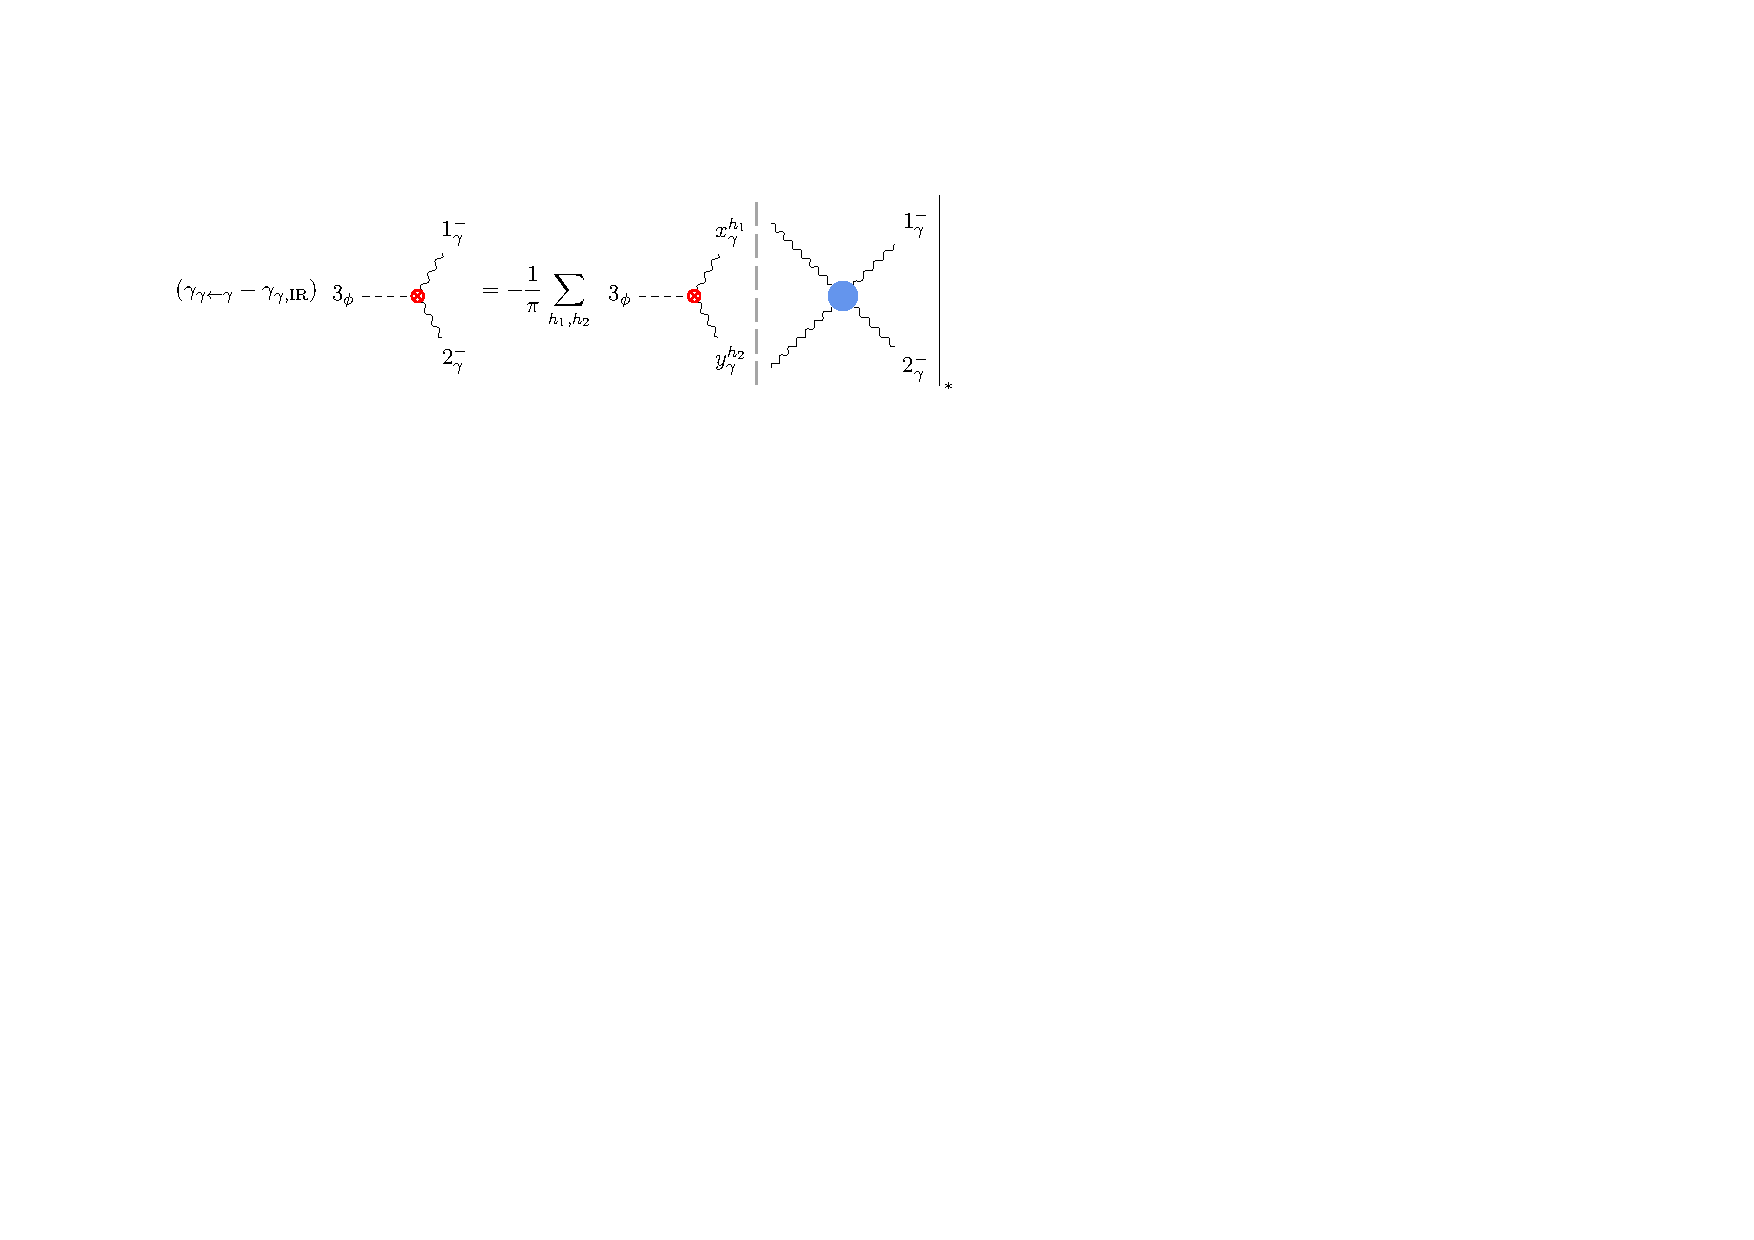
\includegraphics[page=1]{images/ALP_diagrams.pdf}
\caption[Diagrammatic formula for computing $\gamma_{\gamma \leftarrow \gamma}$]{Diagrammatic formula for computing $\gamma_{\gamma \leftarrow \gamma}$.}
\label{fig:ALPgamma_gammagamma}
\end{figure}

The form factor on the left reads
\begin{equation}
    F_\gamma|_*(1^-_\gamma,2^-_\gamma,3_\phi) = -2\frac{\agl{1}{2}^2}{\Lambda}\,,
\end{equation}
while the convolution on the right is expanded as
\begin{equation}
    (\mathcal M F_\gamma)|_*(1^-_\gamma,2^-_\gamma,3_\phi) = \sum_{h_1,h_2}\int \text{dLIPS}_2\, \mathcal M|_*(1^-_\gamma,2^-_\gamma;x_\gamma^{h_1},y^{h_2}_\gamma)F_\gamma|_*(x_\gamma^{h_1},y^{h_2}_\gamma,3_\phi)\,.
\end{equation}
Since the four-photon tree amplitude trivially vanishes for any choice of the helicities,
\begin{equation}
    \mathcal M|_*(1^-_\gamma,2^-_\gamma;x_\gamma^{h_1},y^{h_2}_\gamma) = 0\,,
\end{equation}
we obtain
\begin{equation}
    \gamma_{\gamma \leftarrow \gamma} = \gamma_{\gamma,\text{IR}} = \frac{e^2}{6\pi^2} \sum_f Q_f^2\,,
\end{equation}
where we exploited the expression for $\gamma_{\gamma,\text{IR}}$ derived in
Appendix~\ref{sec:ALPIRphigammagamma}, and $f$ runs over all the fermions of the theory.
We notice that we have successfully derived an expression that is equal to the anomalous
dimension of $e^2$, namely $(\mu/e^2)\, \text{d}e^2/\text{d}\mu$.

\paragraph{\texorpdfstring{$\gamma_{\gamma\leftarrow g}$}{gamma gamma from g}.}
The master formula associated with this matrix element reads
\begin{equation}
    \gamma_{\gamma\leftarrow g} F_\gamma|_*(1^-_\gamma,2^-_\gamma,3_\phi) = -\frac{1}{\pi}(\mathcal M F_g)|_*(1^-_\gamma,2^-_\gamma,3_\phi)
\end{equation}
and is represented in Figure~\ref{fig:ALPgamma_gammag}.

\begin{figure}[h!tb]
\centering
\includegraphics[page=2]{images/ALP_diagrams.pdf}
\caption[Diagrammatic formula for computing $\gamma_{\gamma\leftarrow g}$]{Diagrammatic formula for computing $\gamma_{\gamma\leftarrow g}$.}
\label{fig:ALPgamma_gammag}
\end{figure}

Also in this case the convolution on the right,
\begin{equation}
    (\mathcal M F_g)|_*(1^-_\gamma,2^-_\gamma,3_\phi) = \sum_{h_1,h_2}\int \text{dLIPS}_2\, \mathcal M|_*(1^-_\gamma,2^-_\gamma;x_{g^a}^{h_1},y^{h_2}_{g^b})F_g|_*(x_{g^a}^{h_1},y^{h_2}_{g^b},3_\phi)\,,
\end{equation}
vanishes since
\begin{equation}
    \mathcal M|_*(1^-_\gamma,2^-_\gamma;x_{g^a}^{h_1},y^{h_2}_{g^b}) = 0\,,
\end{equation}
and leads to
\begin{equation}
    \gamma_{\gamma\leftarrow g} = 0\,.
\end{equation}

\paragraph{\texorpdfstring{$\gamma_{\gamma\leftarrow S}$}{gamma gamma from S}.}
The equation linked to this matrix element is given by
\begin{equation}
    \gamma_{\gamma\leftarrow S_{ij}} F_\gamma|_*(1^-_\gamma,2^-_\gamma,3_\phi) = -\frac{1}{\pi}(\mathcal M F_{S_{ij}})|_*(1^-_\gamma,2^-_\gamma,3_\phi)
\end{equation}
and is represented as in Figure~\ref{fig:ALPgamma_gammaS}.

\begin{figure}[h!tb]
\centering
\includegraphics[page=3]{images/ALP_diagrams.pdf}
\caption[Diagrammatic formula for computing $\gamma_{\gamma\leftarrow S_{ij}}$]{Diagrammatic formula for computing $\gamma_{\gamma\leftarrow S_{ij}}$.}
\label{fig:ALPgamma_gammaS}
\end{figure}

From dimensional analysis, we expect
\begin{equation}
    \gamma_{\gamma\leftarrow S_{ij}}=0
\end{equation}
since $[\mathcal O_\gamma]-[\mathcal O_{S_{ij}}]=1$, which is in particular greater than $0$.
This is indeed consistent with the fact that the convolution
\begin{equation}
    (\mathcal M F_{S_{ij}})|_*(1^-_\gamma,2^-_\gamma,3_\phi) = \sum_{h_1,h_2}\int \text{dLIPS}_2\, \mathcal M|_*(1^-_\gamma,2^-_\gamma;x_{f_i}^{h_1},y^{h_2}_{\bar f_j})F_{S_{ij}}|_*(x_{f_i}^{h_1},y^{h_2}_{\bar f_j},3_\phi)
\end{equation}
vanishes due to
\begin{equation}
    \mathcal M|_*(1^-_\gamma,2^-_\gamma;x_{f_i}^{h_1},y^{h_2}_{\bar f_j})=0
\end{equation}
for any choice of $h_1$ and $h_2$.

\paragraph{\texorpdfstring{$\gamma_{\tilde\gamma \leftarrow \tilde\gamma}$, $\gamma_{\tilde\gamma \leftarrow \tilde g}$, and $\gamma_{\tilde\gamma \leftarrow P}$}{gamma gammatilde from gammatilde, gtilde, and P}.}
\label{par:ALPPhiFF}
The anomalous dimensions that contribute to the renormalization of $\phi F\widetilde F$ are
equal to those of $\phi FF$ up to signs that can be determined through the comments leading to
Eq.~\eqref{eq:ALPObs1}:
\begin{align}
    \gamma_{\tilde\gamma \leftarrow \tilde\gamma} &= \gamma_{\gamma \leftarrow \gamma} = \frac{e^2}{6\pi^2}\sum_f Q_f^2 \,,\\
    \gamma_{\tilde\gamma \leftarrow \tilde g} &= \gamma_{\gamma \leftarrow  g} = 0\,,\\
    \gamma_{\tilde\gamma \leftarrow P_{ij}} &= -\gamma_{\gamma \leftarrow S_{ij}} = 0\,.
\end{align}

An interesting feature of the on-shell, unitarity-based method we are employing is that it
makes some properties of the anomalous-dimension matrix manifest.
This is precisely the case for the operator $\phi FF$.
Based on pure symmetry arguments, indeed, one would expect this operator to renormalize like
the electromagnetic fine-structure constant at one-loop level.
The reason for this resides in the fact that the ALP is a pure SM gauge singlet, and hence
$\phi FF$ is expected to renormalize as $FF$.
In turn, as a consequence of Ward identities, this equals the renormalization of
$\alpha_{\text{em}}$.
Such a property is, however, not manifestly apparent at the level of Feynman diagrams.
On the other hand, it is immediately retrieved within the scope of the on-shell method.

\subsubsection{\texorpdfstring{$\phi GG$ and $\phi G\widetilde G$}{phi GG and phi G Gtilde}}
\label{sec:ALPphiGG}

\paragraph{\texorpdfstring{$\gamma_{g \leftarrow g}$}{gamma g from g}.}
The multiplicative renormalization effect of the ALP effective operator $\phi GG$ is encoded in
$\gamma_{g \leftarrow g}$, which can be derived from
\begin{equation}
     (\gamma_{g\leftarrow g}-\gamma_{g,\text{IR}}) F_g|_*(1^-_{g^a},2^-_{g^b},3_\phi) = -\frac{1}{\pi}(\mathcal M F_g)|_*(1^-_{g^a},2^-_{g^b},3_\phi)\,,
\end{equation}
schematized as in Figure~\ref{fig:ALPgamma_gg}.

\begin{figure}[h!tb]
\centering
\includegraphics[page=5]{images/ALP_diagrams.pdf}
\caption[Diagrammatic formula for computing $\gamma_{g\leftarrow g}$]{Diagrammatic formula for computing $\gamma_{g\leftarrow g}$.}
\label{fig:ALPgamma_gg}
\end{figure}

The convolution is now given by
\begin{equation}
    (\mathcal M F_g)|_*(1^-_{g^a},2^-_{g^b},3_\phi) = \sum_{h_1,h_2}\int \text{dLIPS}_2 \, \mathcal M|_*(1^-_{g^a},2^-_{g^b};x^{h_1}_{g^c},y^{h_2}_{g^d})F_g|_*(x^{h_1}_{g^c},y^{h_2}_{g^d},3_\phi)\,,
\end{equation}
where the only contributing amplitude
\begin{equation}
    \mathcal M|_*(1^-_{g^a},2^-_{g^b};x^{-}_{g^c},y^{-}_{g^d})\delta^{cd} = -2C_Ag_s^2 \delta^{ab}\frac{\agl{1}{2}^4}{\agl{1}{x}\agl{x}{2}\agl{2}{y}\agl{y}{1}}
\end{equation}
is multiplied by
\begin{equation}
    F_g|_*(x^{-}_{g^c},y^{-}_{g^d},3_\phi) = -2\delta^{cd}\frac{\agl{x}{y}^2}{\Lambda}\,.
\end{equation}

\subparagraph{Angular integration.}
The calculation of the phase-space integral with the angular parameterization is as follows.
The product reads
\begin{equation}
    \mathcal M|_*(1^-_{g^a},2^-_{g^b};x^{-}_{g^c},y^{-}_{g^d})F_g|_*(x^{-}_{g^c},y^{-}_{g^d},3_\phi) = -4C_Ag_s^2 \delta^{ab} \frac{\agl{1}{2}^2}{\Lambda} \frac{1}{\cos^2\theta \sin^2\theta}\,,
\end{equation}
yielding
\begin{equation}
    (\mathcal M F_g)|_*(1^-_{g^a},2^-_{g^b},3_\phi) = -4C_Ag_s^2 \delta^{ab} \frac{\agl{1}{2}^2}{\Lambda} \frac{1}{16\pi}\int_0^{\pi/2}2 \sin\theta\cos\theta\,\text{d}\theta\, \frac{1}{\cos^2\theta \sin^2\theta}\,.
\end{equation}
Therefore, by making use of the expression for $\gamma_{g,\text{IR}}$ derived in
Appendix~\ref{sec:ALPIRphigg} and reported in Eq.~\eqref{eq:ALPgammaIRgluon_angular}, we obtain
\begin{align}
    \gamma_{g\leftarrow g} &= \gamma_{g,\text{IR}} - C_A\frac{g_s^2}{8\pi^2}  \int_0^{\pi/2}2\sin\theta\cos\theta \, \text{d}\theta \, \frac{1}{\cos^2\theta\sin^2\theta}\nonumber \\
    &= T_F\frac{g_s^2}{6\pi^2}\sum_f c_f^2 - C_A\frac{g_s^2}{8\pi^2}  \int_0^{\pi/2}2\sin\theta\cos\theta \, \text{d}\theta \, \frac{1 -\cos^8\theta- \sin^8\theta}{\cos^2\theta\sin^2\theta}\nonumber \\
    &= -\frac{g_s^2}{8\pi^2}\bigg(\frac{11}{3}C_A -\frac{4}{3}T_F\sum_fc_f^2\bigg)\,,
\end{align}
which is equal to the anomalous dimension of $g_s^2$, namely
$(\mu/g_s^2)\,\text{d}g_s^2/\text{d}\mu$, since $\sum_f c_f^2$ denotes the number of quarks.

\subparagraph{Stokes integration.}
The calculation of the phase-space integral with the Stokes parameterization is as follows.
The product reads
\begin{equation}
    \mathcal M|_*(1^-_{g^a},2^-_{g^b};x^{-}_{g^c},y^{-}_{g^d})F_g|_*(x^{-}_{g^c},y^{-}_{g^d},3_\phi) = -4C_Ag_s^2 \delta^{ab} \frac{\agl{1}{2}^2}{\Lambda} \frac{(1+z\bar z)^2}{z\bar z }
\end{equation}
and vanishes after performing the Stokes integration.
Therefore, also in this case, the anomalous dimension is given by $\gamma_{g,\text{IR}}$,
derived in Appendix \ref{sec:ALPIRphigg} and reported in
Eq.\ \eqref{eq:ALPgammaIRgluon_stokes}:
\begin{equation}
    \gamma_{g\leftarrow g} = \gamma_{g,\text{IR}}
    = -\frac{g_s^2}{8\pi^2}\bigg(\frac{11}{3}C_A -\frac{4}{3}T_F\sum_fc_f^2\bigg)\,.
\end{equation}

\paragraph{\texorpdfstring{$\gamma_{g\leftarrow \gamma}$}{gamma g from gamma}.}
The master formula for computing $\gamma_{g\leftarrow \gamma}$ is
\begin{equation}
    \gamma_{g\leftarrow \gamma} F_g|_*(1^-_{g^a},2^-_{g^b},3_\phi) = -\frac{1}{\pi}(\mathcal M F_\gamma)|_*(1^-_{g^a},2^-_{g^b},3_\phi)\,,
\end{equation}
and its diagrammatic expression is reported in Figure~\ref{fig:ALPgamma_ggamma}.

\begin{figure}[h!tb]
\centering
\includegraphics[page=4]{images/ALP_diagrams.pdf}
\caption[Diagrammatic formula for computing $\gamma_{g\leftarrow \gamma}$]{Diagrammatic formula for computing $\gamma_{g\leftarrow \gamma}$.}
\label{fig:ALPgamma_ggamma}
\end{figure}

On the left, the form factor associated with $\phi GG$ reads
\begin{equation}
    F_g|_*(1^-_{g^a},2^-_{g^b},3_\phi) = -2\delta^{ab}\frac{\agl{1}{2}^2}{\Lambda}\,,
\end{equation}
and the convolution on the right is expanded as
\begin{equation}
    (\mathcal M F_\gamma)|_*(1^-_{g^a},2^-_{g^b},3_\phi) = \sum_{h_1,h_2}\int \text{dLIPS}_2 \, \mathcal M|_*(1^-_{g^a},2^-_{g^b};x^{h_1}_\gamma,y^{h_2}_\gamma)F_\gamma|_*(x^{h_1}_\gamma,y^{h_2}_\gamma,3_\phi)\,.
\end{equation}
Since the amplitudes trivially vanish,
\begin{equation}
    \mathcal M|_*(1^-_{g^a},2^-_{g^b};x^{h_1}_\gamma,y^{h_2}_\gamma) = 0\,,
\end{equation}
we obtain
\begin{equation}
    \gamma_{g\leftarrow \gamma} = 0\,.
\end{equation}

\paragraph{\texorpdfstring{$\gamma_{g\leftarrow S}$}{gamma g from S}.}
The formula corresponding to $\gamma_{g\leftarrow S_{ij}}$ is
\begin{equation}
    \gamma_{g\leftarrow S_{ij}} F_g|_*(1^-_{g^a},2^-_{g^b},3_\phi) = -\frac{1}{\pi}(\mathcal M F_{S_{ij}})|_*(1^-_{g^a},2^-_{g^b},3_\phi)
\end{equation}
and is reported diagrammatically in Figure~\ref{fig:ALPgamma_gS}.

\begin{figure}[h!tb]
\centering
\includegraphics[page=6]{images/ALP_diagrams.pdf}
\caption[Diagrammatic formula for computing $\gamma_{g\leftarrow S_{ij}}$]{Diagrammatic formula for computing $\gamma_{g\leftarrow S_{ij}}$.}
\label{fig:ALPgamma_gS}
\end{figure}

Also in this case, analogously to $\gamma_{\gamma\leftarrow S_{ij}}$, we expect
\begin{equation}
    \gamma_{g\leftarrow S_{ij}}=0
\end{equation}
because $[\mathcal O_g]-[\mathcal O_{S_{ij}}]=1>0$.
This is indeed consistent with the fact that the convolution
\begin{equation}
    (\mathcal M F_{S_{ij}})|_*(1^-_{g^a},2^-_{g^b},3_\phi) = \sum_{h_1,h_2}\int \text{dLIPS}_2\, \mathcal M|_*(1^-_{g^a},2^-_{g^b};x_{f_i^I}^{h_1},y^{h_2}_{\bar f_j^J})F_{S_{ij}}|_*(x_{f_i^I}^{h_1},y^{h_2}_{\bar f_j^J},3_\phi)
\end{equation}
vanishes due to
\begin{equation}
    \mathcal M|_*(1^-_{g^a},2^-_{g^b};x_{f_i^I}^{h_1},y^{h_2}_{\bar f_j^J})=0
\end{equation}
for any choice of $h_1$ and $h_2$.

\paragraph{\texorpdfstring{$\gamma_{\tilde g \leftarrow \tilde\gamma}$, $\gamma_{\tilde g \leftarrow \tilde g}$, and $\gamma_{\tilde g \leftarrow P}$}{gamma gtilde from gammatilde, gtilde, and P}.}
\label{par:ALPPhiGG}
Once again, the anomalous dimensions that contribute to the renormalization of
$\phi G\widetilde G$ are equal to those of $\phi GG$ up to signs that can be determined through
the comments leading to Eq.~\eqref{eq:ALPObs1}:
\begin{align}
    \gamma_{\tilde g \leftarrow \tilde \gamma } &= \gamma_{ g \leftarrow  \gamma } = 0\,,\\
    \gamma_{\tilde g \leftarrow \tilde g } &= \gamma_{ g \leftarrow  g } = -\frac{g_s^2}{8\pi^2}\bigg(\frac{11}{3}C_A -\frac{4}{3}T_F\sum_fc_f^2\bigg) \,,\\
    \gamma_{\tilde g \leftarrow P_{ij} } &= -\gamma_{ g \leftarrow  S_{ij} } = 0\,.
\end{align}

\subsubsection{Renormalization-Group Equations}
\label{sec:ALPRGEcouplings}

In this section, we have successfully reproduced some known results in the literature regarding
the renormalization of the CP-violating ALP
Lagrangian~\cite{Bauer:2021mvw,Chala:2020wvs,DasBakshi:2023lca}.
Here we report a summary of our results:
\begin{gather}
    \mu\dv[]{\mathcal C_\gamma}{\mu} = \frac{e^2}{6\pi^2}\mathcal C_\gamma \sum_f Q_f^2\,,
    \qquad
    \mu\dv[]{\widetilde{\mathcal C}_\gamma}{\mu} = \frac{e^2}{6\pi^2}\widetilde{\mathcal C}_\gamma \sum_f Q_f^2\,,
    \\
    \mu\dv[]{\mathcal C_g}{\mu} = -\frac{g_s^2}{8\pi^2} \bigg(\frac{11}{3} C_A - \frac{4}{3}T_F \sum_f c_f^2\bigg) \mathcal C_g\,,
    \qquad
    \mu\dv[]{\widetilde{\mathcal C}_g}{\mu} = -\frac{g_s^2}{8\pi^2} \bigg(\frac{11}{3} C_A - \frac{4}{3}T_F \sum_f c_f^2\bigg) \widetilde{\mathcal C}_g \,,
    \\
    \mu\dv[]{\mathcal Y_S^{ij}}{\mu} = -\frac{3}{8\pi^2}\left(e^2Q_f^2+C_Fg_s^2c_f^2 \right)\mathcal Y_S^{ij} + \frac{3}{2\pi^2}\frac{m_i}{\Lambda}\left(e^2Q_f^2 \mathcal C_\gamma + C_F g_s^2 c_f^2 \mathcal C_g\right)\delta^{ij}\,,\\
    \mu\dv[]{\mathcal Y_P^{ij}}{\mu} = -\frac{3}{8\pi^2}\left(e^2Q_f^2 +C_Fg_s^2c_f^2 \right)\mathcal Y_P^{ij} - \frac{3}{2\pi^2}\frac{m_i}{\Lambda}\left(e^2Q_f^2 \widetilde{\mathcal C}_\gamma + C_F g_s^2 c_f^2 \widetilde{\mathcal C}_g\right)\delta^{ij}\,.
\end{gather}

%%%%%%%%%%%%%%%%
\subsection{Renormalization of Standard Model Effective Operators Below the Electroweak Scale}
\label{sec:ALPLEFT}
%%%%%%%%%%%%%%%%

The phenomenological consequences of the ALP-SM interactions encoded in
Eq.~\eqref{eq:ALPLag} are rich and diverse.
Of particular interest among these are the indirect effects on precision observables that are
induced by the virtual exchange of an ALP.
Such precision observables entail not only CP-violating probes, such as the electric dipole
moment of particles, nucleons, nuclei, and molecules, but also CP-conserving ones, as for
instance the anomalous magnetic moment of leptons~\cite{Marciano:2016yhf,DiLuzio:2020oah}.
Since the impact on these physical observables is generated at the quantum level, a natural
expectation is that their size can be determined by the leading logarithms that emerge from the
solution of the RGEs.
This expectation is rooted in the large separation of scales between the energies at which
experiments are performed and those at which the effective Lagrangian is defined.

The resulting CP-even $SU(3)_c \times U(1)_{\text{em}}$ invariant Lagrangian,
$\mathcal{L}^{\text{even}}_{\text{CP}}$, that is generated by integrating out the ALP at
one-loop level reads
\begin{align}
\label{eq:ALPCPELag}
 \mathcal{L}^{\text{even}}_{\text{CP}} &=
\frac{c_{\rm M}^{ij}}{\Lambda} \, \bar{f}_i \sigma^{\mu\nu} f_j \, F_{\mu\nu} +  \frac{c_{\rm CM}^{ij}}{\Lambda} \, \bar{f}_i \sigma^{\mu\nu} T^a f_j \, G^a_{\mu\nu} + \frac{D_G}{3\Lambda^2} f^{abc} G_\mu^{a \nu} G_{\nu}^{b \rho} G_{\rho}^{c \mu} \nonumber \\
& \quad +
\frac{c_{LL1}^{ijkl}}{\Lambda^2}(\bar f_{Li} \gamma^\mu f_{Lj})(\bar f'_{Lk}\gamma_\mu f'_{Ll}) + \frac{c_{LL8}^{ijkl}}{\Lambda^2}(\bar f_{Li} \gamma^\mu T^a f_{Lj})(\bar f'_{Lk}\gamma_\mu T^a f'_{Ll})\nonumber \\
& \quad +
\frac{c_{RR1}^{ijkl}}{\Lambda^2}(\bar f_{Ri} \gamma^\mu f_{Rj})(\bar f'_{Rk}\gamma_\mu f'_{Rl}) +
\frac{c_{RR8}^{ijkl}}{\Lambda^2}(\bar f_{Ri} \gamma^\mu T^a f_{Rj})(\bar f'_{Rk}\gamma_\mu T^a f'_{Rl})\nonumber \\
& \quad +
\frac{c_{LR1}^{ijkl}}{\Lambda^2}(\bar f_{Li} \gamma^\mu f_{Lj})(\bar f'_{Rk}\gamma_\mu f'_{Rl}) +
\frac{c_{LR8}^{ijkl}}{\Lambda^2}(\bar f_{Li} \gamma^\mu T^a f_{Lj})(\bar f'_{Rk}\gamma_\mu T^a f'_{Rl})
\,.
\end{align}
The corresponding CP-odd Lagrangian, $\mathcal{L}^{\text{odd}}_{\text{CP}}$, is given by
\begin{align}
\label{eq:ALPCPOLag}
 \mathcal{L}^{\text{odd}}_{\text{CP}} =
 \frac{c_{\rm E}^{ij}}{\Lambda} \, \bar{f}_i \sigma^{\mu\nu} i\gamma_5 f_j \, F_{\mu\nu} +  \frac{c_{\rm CE}^{ij}}{\Lambda} \, \bar{f}_i \sigma^{\mu\nu} i\gamma_5 T^a f_j \, G^a_{\mu\nu} + \frac{d_G}{3\Lambda^2} f^{abc} G_\mu^{a \nu} G_{\nu}^{b \rho} \widetilde G_{\rho}^{c \mu}\,.
\end{align}
Here, $\sigma_{\mu\nu} = \frac{i}{2}[\gamma_\mu,\gamma_\nu]$.
Notice that in the above Lagrangians we have neglected operators which emerge by integrating
out the ALP at tree level, such as $(\bar{f} f)( \bar{f}' f')$, $GGGG$, and so on.
In fact, in this case, RGE effects are fully accounted for by evaluating the effective ALP
couplings of Eqs.~\eqref{eq:ALPLagA} and \eqref{eq:ALPLagB} at the ALP mass scale.

The objective of this section is to evaluate the Wilson coefficients of the above Lagrangians
that are generated by running effects from $\Lambda$ down to the ALP mass scale.

\subsubsection{\texorpdfstring{$GG\widetilde G$ and $GGG$}{GG Gtilde and GGG}}
\label{sec:ALPGGG}

\paragraph{\texorpdfstring{$\gamma_{\tilde G^3\leftarrow g,\tilde g}$}{gamma G3tilde from g, gtilde}.}
We define the Weinberg dimension-six operator as
\begin{equation}
    \mathcal O_{\tilde G^3} = \frac{1}{3}f^{abc}G_\mu^{a \nu} G_{\nu}^{b \rho} \widetilde G_{\rho}^{c \mu}\,.
\end{equation}
The renormalization of the corresponding Wilson coefficient induced by the operators $\phi GG$
and $\phi G\widetilde G$ at one-loop order can be evaluated from
\begin{equation}\label{eq:ALPmastertildeG3}
    \gamma_{\tilde G^3\leftarrow g,\tilde g}F_{\tilde G^3}|_*(1^-_{g^a},2^-_{g^b},3^-_{g^c})=-\frac{1}{\pi}\left. \frac{\partial}{\partial \mathcal C_g} \right|_{\mathcal C_g = 0} (\mathcal M F_{\tilde g})|_{*,\mathcal C_g \neq  0}(1^-_{g^a},2^-_{g^b},3^-_{g^c})\,,
\end{equation}
which diagrammatically reads as in Figure~\ref{fig:ALPgammatildeG3}.

\begin{figure}[h!tb]
\centering
\includegraphics[page=9]{images/ALP_diagrams.pdf}
\caption[Diagrammatic formula for computing $\gamma_{\tilde G^3\leftarrow g,\tilde g}$]{Diagrammatic formula for computing $\gamma_{\tilde G^3\leftarrow g,\tilde g}$.}
\label{fig:ALPgammatildeG3}
\end{figure}

The minimal form factor of $\mathcal O_{\tilde G^3}$ reads
\begin{equation}
    F_{\tilde G^3}|_*(1^-_{g^a},2^-_{g^b},3^-_{g^c})=\frac{\sqrt 2}{\Lambda^2}f^{abc}\agl{1}{2}\agl{2}{3}\agl{3}{1}\,,
\end{equation}
while the convolution can be written as
\begin{equation}
    (\mathcal M F_{\tilde g})|_{*,\mathcal C_g \neq  0}(1^-_{g^a},2^-_{g^b},3^-_{g^c}) = 3 \sum_{h}\int \text{dLIPS}_2\, \mathcal{M}|_{*,\mathcal C_g \neq  0}(1^-_{g^a},2^-_{g^b};x_\phi,y^h_{g^d})
    F_{\tilde g}|_*(x_\phi,y^h_{g^d},3^-_{g^c})\,,
\end{equation}
where the factor $3$ accounts for all the permutations of the external gluons.
The only helicity $h$ that gives a non-zero contribution is the negative one, since
$F_{\tilde g}|_*(x_\phi,y^+_{g^d},3^-_{g^c}) = 0$.
The amplitude with $\mathcal C_g\neq 0$ and all the other Wilson coefficients turned off, and
the minimal form factor of $\mathcal O_{\tilde g}$, are, respectively, given by
\begin{align}
    \mathcal{M}|_{*,\mathcal C_g \neq  0}(1^-_{g^a},2^-_{g^b};x_\phi,y^-_{g^d}) &= 2i\sqrt{2}g_s \frac{\mathcal C_g}{\Lambda}f^{abd}\frac{ \agl{1}{2}^3 }{ \agl{1}{y} \agl{2}{y}}\,,\\
    F_{\tilde g}|_*(x_\phi,y^-_{g^d},3^-_{g^c}) &= -\frac{2i}{\Lambda}\delta^{cd}\agl{3}{y}^2\,.
\end{align}

\subparagraph{Angular integration.}
Using the angular parameterization for the phase-space integral, the amplitude reads
\begin{equation}\label{eq:ALPamplitudeCg}
    \mathcal{M}|_{*,\mathcal C_g \neq  0}(1^-_{g^a},2^-_{g^b};x_\phi,y^-_{g^d}) = -2i\sqrt{2}g_s \frac{\mathcal C_g}{\Lambda}f^{abd}\agl{1}{2}\frac{1}{ \cos\theta\sin\theta}e^{i\varphi}\,.
\end{equation}
The integration in the azimuthal angle $\varphi$ only involves
\begin{align}
    \int_0^{2\pi}\frac{\text{d}\varphi}{2\pi}\,F_{\tilde g}|_*(x_\phi,y^-_{g^d},3^-_{g^c}) e^{i\varphi} &=
    -\frac{2i}{\Lambda}\delta^{cd}\int_0^{2\pi}\frac{\text{d}\varphi}{2\pi}\, (\agl{3}{1}e^{-i\varphi}\sin\theta + \agl{3}{2}\cos\theta)^2e^{i\varphi}
    \nonumber \\&=\frac{4i}{\Lambda}\delta^{cd}\agl{2}{3}\agl{3}{1}\cos\theta\sin\theta\,,\label{eq:ALPphiintegral}
\end{align}
where $\int_0^{2\pi} \text{d}\varphi\,e^{in\varphi}=2\pi\delta_{0n}$ has been used.
Therefore, the $\theta$ dependences of Eqs.~\eqref{eq:ALPamplitudeCg} and
\eqref{eq:ALPphiintegral} cancel each other, and we are left with a trivial integral in
$\theta$, which leads to
\begin{align}
    (\mathcal M F_{\tilde g})|_{*,\mathcal C_g \neq  0}(1^-_{g^a},2^-_{g^b},3^-_{g^c}) &= 3\times 8\sqrt 2 g_s \frac{\mathcal C_g}{\Lambda^2}f^{abc}\agl{1}{2}\agl{2}{3} \agl{3}{1} \frac{1}{8\pi}\int_0^{\pi/2}2\sin\theta\cos\theta\,\text{d}\theta \nonumber \\
    &= \frac{3\sqrt{2}}{\pi\Lambda^2} g_s\mathcal  C_gf^{abc} \agl{1}{2}\agl{2}{3} \agl{3}{1}\,.
\end{align}

\subparagraph{Stokes integration.}
Using the Stokes parameterization for the phase-space integral, the amplitude reads
\begin{equation}
    \mathcal{M}|_{*,\mathcal C_g \neq  0}(1^-_{g^a},2^-_{g^b};x_\phi,y^-_{g^d}) = 2i\sqrt{2}g_s \frac{\mathcal C_g}{\Lambda}f^{abd}\agl{1}{2}\frac{1+z\bar z}{ z}\,,
\end{equation}
which implies
\begin{equation}
    (\mathcal M F_{\tilde g})|_{*,\mathcal C_g \neq  0}(1^-_{g^a},2^-_{g^b},3^-_{g^c}) =  \frac{3\sqrt{2}}{\pi\Lambda^2} g_s\mathcal  C_gf^{abc} \agl{1}{2}\agl{2}{3} \agl{3}{1}\,.
\end{equation}
Finally, from the master formula of Eq.~\eqref{eq:ALPmastertildeG3}, we obtain
\begin{equation}
\label{eq:ALPgammatildeG3}
    \gamma_{\tilde G^3\leftarrow g,\tilde g} = -\frac{3g_s}{\pi^2}\,.
\end{equation}

\paragraph{\texorpdfstring{$\gamma_{G^3\leftarrow g, g}$ and $\gamma_{G^3\leftarrow \tilde g, \tilde g}$}{gamma G3 from gg and gtilde gtilde}.}
\label{par:ALPGGG}
The beta function associated with the Wilson coefficient of the CP-even operator
\begin{equation}
    \mathcal O_{G^3} = \frac{1}{3}f^{abc}G_\mu^{a \nu} G_{\nu}^{b \rho} G_{\rho}^{c \mu}
\end{equation}
receives contributions from double insertions of the operators $\phi GG$ and
$\phi G\widetilde G$.
The corresponding anomalous dimensions $\gamma_{ G^3\leftarrow g, g}$ and
$\gamma_{ G^3\leftarrow \tilde g,\tilde g}$ can be computed via
\begin{align}
    \gamma_{ G^3\leftarrow g, g}F_{ G^3}|_*(1^-_{g^a},2^-_{g^b},3^-_{g^c})&=-\frac{1}{\pi}\left. \frac{\partial}{\partial \mathcal C_g} \right|_{\mathcal C_g = 0} (\mathcal M F_{g})|_{*,\mathcal C_g \neq  0}(1^-_{g^a},2^-_{g^b},3^-_{g^c})\,, \\
    \gamma_{ G^3\leftarrow \tilde g,\tilde g}F_{ G^3}|_*(1^-_{g^a},2^-_{g^b},3^-_{g^c})&=-\frac{1}{\pi}\left. \frac{\partial}{\partial \widetilde{\mathcal{C}}_g} \right|_{\widetilde{\mathcal{C}}_g = 0} (\mathcal M F_{\tilde g})|_{*,\widetilde{\mathcal{C}}_g \neq  0}(1^-_{g^a},2^-_{g^b},3^-_{g^c})\,,
\end{align}
respectively, and both can be straightforwardly related to the anomalous dimension
$\gamma_{\tilde G^3\leftarrow g,\tilde g}$ in Eq.~\eqref{eq:ALPgammatildeG3}.
Indeed, by taking into account that
\begin{align}
    F_{ G^3}|_*(1^-_{g^a},2^-_{g^b},3^-_{g^c}) &= -i F_{\tilde G^3}|_*(1^-_{g^a},2^-_{g^b},3^-_{g^c})\,, \\
    F_{g}|_*(x_\phi,y^-_{g^d},3^-_{g^c}) &=-i F_{\tilde g}|_*(x_\phi,y^-_{g^d},3^-_{g^c})\,,\\
    \frac{\partial}{\partial \widetilde{\mathcal{C}}_g}\mathcal{M}|_{*,\widetilde{\mathcal{C}}_g \neq  0}(1^-_{g^a},2^-_{g^b};x_\phi,y^-_{g^d})&= i \frac{\partial}{\partial \mathcal{C}_g} \mathcal{M}|_{*,\mathcal C_g \neq  0}(1^-_{g^a},2^-_{g^b};x_\phi,y^-_{g^d})\,,
\end{align}
we obtain
\begin{equation}
\label{eq:ALPGGG_AD}
    \gamma_{ G^3\leftarrow g, g} =- \gamma_{ G^3\leftarrow \tilde g, \tilde g} = \gamma_{ \tilde G^3\leftarrow g, \tilde g} = -\frac{3g_s}{\pi^2}\,.
\end{equation}

\subsubsection{\texorpdfstring{$\bar f \sigma\!\cdot\! F i\gamma_5 f$ and $\bar f \sigma\!\cdot\! F f$}{fbar sigma F i gamma5 f and fbar sigma F f}}
\label{sec:ALPdipole}

\paragraph{\texorpdfstring{$\gamma_{\mathrm{E}\leftarrow S,\tilde\gamma}$}{gamma E from S, gammatilde}.}
The first anomalous dimension $\gamma_{\text{E}_{ij}\leftarrow S_{kl},\tilde\gamma}$ of the
electric dipole operator
\begin{equation}
    \mathcal O_{\text{E}_{ij}} =
    \bar f_i \sigma^{\mu\nu}i\gamma_5 f_j F_{\mu\nu}
\end{equation}
is induced by the ALP operators $\phi\, \bar f_k f_l$ and $\phi F\widetilde F$.
The corresponding master formula reads
\begin{equation}
    \gamma_{\text{E}_{ij}\leftarrow S_{kl},\tilde\gamma} F_{\text{E}_{ij}}|_*(1^-_{f_i},2^-_{\bar f_j},3^-_\gamma) = -\frac{1}{\pi}\left.\frac{\partial}{\partial \mathcal Y_S^{kl}}\right|_{\mathcal Y_S^{kl}=0}(\mathcal M F_{\tilde\gamma})|_{*,\mathcal Y_S^{kl}\neq 0}(1^-_{f_i},2^-_{\bar f_j},3^-_\gamma)\,,
\end{equation}
whose diagrammatic expression is provided in Figure~\ref{fig:ALPgammaEDM}.

\begin{figure}[h!tb]
\centering
\includegraphics[width=\linewidth,page=10]{images/ALP_diagrams.pdf}
\caption[Diagrammatic formula for computing $\gamma_{\text{E}_{ij}\leftarrow S_{kl},\tilde\gamma}$]{Diagrammatic formula for computing $\gamma_{\text{E}_{ij}\leftarrow S_{kl},\tilde\gamma}$.}
\label{fig:ALPgammaEDM}
\end{figure}

On the left-hand side we have the form factor of the electric dipole operator
\begin{equation}
    F_{\text{E}_{ij}}|_*(1^-_{f_i},2^-_{\bar f_j},3^-_\gamma) = -\frac{2i \sqrt{2}}{\Lambda} \agl{1}{3}\agl{2}{3}\,,
\end{equation}
while, on the right-hand side, the convolution reads
\begin{equation}
    (\mathcal M F_{\tilde\gamma})|_{*,\mathcal Y_S^{kl}\neq 0}(1^-_{f_i},2^-_{\bar f_j},3^-_\gamma) = \sum_{h} \int \text{dLIPS}_2 \, \mathcal M|_{*,\mathcal Y_S^{kl}\neq 0}(1^-_{f_i},2^-_{\bar f_j};x_\phi,y^h_\gamma) F_{\tilde\gamma}|_*(x_\phi,y^h_\gamma,3_\gamma^-)\,,
\end{equation}
where the only non-vanishing amplitude is
\begin{equation}
    \mathcal M|_{*,\mathcal Y_S^{kl}\neq 0}(1^-_{f_i},2^-_{\bar f_j};x_\phi,y^-_\gamma) =  -\sqrt 2 eQ_f \mathcal Y_S^{kl}\delta^{ik}\delta^{jl} \frac{\agl{1}{2}^2}{\agl{1}{y}\agl{y}{2}}
\end{equation}
and is multiplied by
\begin{equation}
    F_{\tilde\gamma}|_*(x_\phi,y^-_\gamma,3_\gamma^-) = -\frac{2i}{\Lambda}\agl{3}{y}^2\,.
\end{equation}

\subparagraph{Angular integration.}
The calculation of the phase-space integral with the angular parameterization is as follows.
The amplitude reads
\begin{equation}
    \mathcal M|_{*,\mathcal Y_S^{kl}\neq 0}(1^-_{f_i},2^-_{\bar f_j};x_\phi,y^-_\gamma) =  -\sqrt 2 eQ_f \mathcal Y_S^{kl}\delta^{ik}\delta^{jl} \frac{1}{\cos\theta \sin\theta}e^{i\varphi}\,,
\end{equation}
and thus the integration in the azimuthal angle $\varphi$ only involves
\begin{equation}
    \int_0^{2\pi}\frac{\text{d}\varphi}{2\pi}\,F_{\tilde\gamma}|_*(x_\phi,y^-_\gamma,3_\gamma^-)e^{i\varphi} = - \frac{4i}{\Lambda}\agl{2}{3}\agl{1}{3}\cos\theta\sin\theta\,.
\end{equation}
Then, the remaining integral is simply
\begin{align}
    (\mathcal M F_{\tilde\gamma})|_{*,\mathcal Y_S^{kl}\neq 0}(1^-_{f_i},2^-_{\bar f_j},3^-_\gamma) &=  \frac{4 i\sqrt 2}{\Lambda}  eQ_f \mathcal Y_S^{kl}\delta^{ik}\delta^{jl}  \agl{2}{3}\agl{1}{3} \frac{1}{8\pi}\int_0^{\pi/2}2\sin\theta\cos\theta\,\text{d}\theta \nonumber \\
    &=  \frac{ i\sqrt 2}{2\pi\Lambda}  eQ_f \mathcal Y_S^{kl}\delta^{ik}\delta^{jl}  \agl{2}{3}\agl{1}{3}\,,
\end{align}
which leads to
\begin{equation}\label{eq:ALPgammaEfromSgammatilde}
    \gamma_{\text{E}_{ij}\leftarrow S_{kl},\tilde\gamma} =  \frac{eQ_f }{4\pi^2}\delta^{ik}\delta^{jl}\,.
\end{equation}

\subparagraph{Stokes integration.}
Using the Stokes parameterization, the amplitude reads
\begin{equation}
    \mathcal M|_{*,\mathcal Y_S^{kl}\neq 0}(1^-_{f_i},2^-_{\bar f_j};x_\phi,y^-_\gamma) =  \sqrt 2 eQ_f \mathcal Y_S^{kl}\delta^{ik}\delta^{jl} \frac{1+z \bar z}{z} \, ,
\end{equation}
and combining it with the form factor we get
\begin{equation}
    (\mathcal M F_{\tilde\gamma})|_{*,\mathcal Y_S^{kl}\neq 0}(1^-_{f_i},2^-_{\bar f_j},3^-_\gamma)
    =  \frac{ i\sqrt 2}{2\pi\Lambda}  eQ_f \mathcal Y_S^{kl}\delta^{ik}\delta^{jl}  \agl{2}{3}\agl{1}{3}\,,
\end{equation}
which leads to Eq.~\eqref{eq:ALPgammaEfromSgammatilde}.

\paragraph{\texorpdfstring{$\gamma_{\mathrm{E}\leftarrow P,\gamma}$}{gamma E from P, gamma}.}
The second anomalous dimension $\gamma_{\text{E}_{ij}\leftarrow P_{kl},\gamma}$, corresponding
to the insertion of the ALP operators $\phi\, \bar f_k i\gamma_5 f_l$ and $\phi FF$, can be
obtained from the master formula
\begin{equation}
    \gamma_{\text{E}_{ij}\leftarrow P_{kl},\gamma} F_{\text{E}_{ij}}|_*(1^-_{f_i},2^-_{\bar f_j},3^-_\gamma) = -\frac{1}{\pi}\left.\frac{\partial}{\partial \mathcal Y_P^{kl}}\right|_{\mathcal Y_P^{kl}=0}(\mathcal M F_{\gamma})|_{*,\mathcal Y_P^{kl}\neq 0}(1^-_{f_i},2^-_{\bar f_j},3^-_\gamma)\,,
\end{equation}
and, since the identities
\begin{align}
    F_{\gamma}|_*(x_\phi,y^-_\gamma,3_\gamma^-) &= -i F_{\tilde\gamma}|_*(x_\phi,y^-_\gamma,3_\gamma^-) \,,
    \label{eq:ALPF_gamma_identity}\\
    \frac{\partial}{\partial \mathcal Y_P^{kl}}\mathcal M|_{*,\mathcal Y_P^{kl}\neq 0}(1^-_{f_i},2^-_{\bar f_j};x_\phi,y^-_\gamma)&=-i \frac{\partial}{\partial \mathcal Y_S^{kl}} \mathcal M|_{*,\mathcal Y_S^{kl}\neq 0}(1^-_{f_i},2^-_{\bar f_j};x_\phi,y^-_\gamma)\label{eq:ALPamplitudeyukawaidentity}
\end{align}
hold, we can relate it to $\gamma_{\text{E}_{ij}\leftarrow S_{kl},\tilde\gamma}$, concluding
that
\begin{equation}
    \gamma_{\text{E}_{ij}\leftarrow P_{kl},\gamma} = - \gamma_{\text{E}_{ij}\leftarrow S_{kl},\tilde\gamma}= -\frac{eQ_f }{4\pi^2}\delta^{ik}\delta^{jl}\,.
\end{equation}

\paragraph{\texorpdfstring{$\gamma_{\mathrm{M}\leftarrow P,\tilde \gamma}$ and $\gamma_{\mathrm{M}\leftarrow S,\gamma}$}{gamma M from P, gammatilde and S, gamma}.}
The magnetic dipole operator is defined as
\begin{equation}
    \mathcal O_{\text{M}_{ij}} = \bar f_i \sigma^{\mu\nu}f_j F_{\mu\nu}\,,
\end{equation}
and the corresponding anomalous dimensions $\gamma_{\text{M}_{ij}\leftarrow S_{kl},\gamma}$ and
$\gamma_{\text{M}_{ij}\leftarrow P_{kl},\tilde\gamma}$ can be obtained from the master
formulae
\begin{align}
    \gamma_{\text{M}_{ij}\leftarrow S_{kl},\gamma} F_{\text{M}_{ij}}|_*(1^-_{f_i},2^-_{\bar f_j},3^-_\gamma) &= -\frac{1}{\pi}\left.\frac{\partial}{\partial \mathcal Y_S^{kl}}\right|_{\mathcal Y_S^{kl}=0}(\mathcal M F_{\gamma})|_{*,\mathcal Y_S^{kl}\neq 0}(1^-_{f_i},2^-_{\bar f_j},3^-_\gamma)\,, \\
    \gamma_{\text{M}_{ij}\leftarrow P_{kl},\tilde\gamma} F_{\text{M}_{ij}}|_*(1^-_{f_i},2^-_{\bar f_j},3^-_\gamma) &= -\frac{1}{\pi}\left.\frac{\partial}{\partial \mathcal Y_P^{kl}}\right|_{\mathcal Y_P^{kl}=0}(\mathcal M F_{\tilde\gamma})|_{*,\mathcal Y_P^{kl}\neq 0}(1^-_{f_i},2^-_{\bar f_j},3^-_\gamma)\,.
\end{align}
If we exploit the identity
\begin{equation}
    F_{\text{M}_{ij}}|_*(1^-_{f_i},2^-_{\bar f_j},3^-_\gamma) =i F_{\text{E}_{ij}}|_*(1^-_{f_i},2^-_{\bar f_j},3^-_\gamma)\,,
\end{equation}
as well as those in Eqs.~\eqref{eq:ALPF_gamma_identity} and
\eqref{eq:ALPamplitudeyukawaidentity}, we can relate both of them to
$\gamma_{\text{E}_{ij}\leftarrow S_{kl},\tilde\gamma}$, concluding that
\begin{equation}
    \gamma_{\text{M}_{ij}\leftarrow P_{kl},\tilde\gamma}=
    \gamma_{\text{M}_{ij}\leftarrow S_{kl},\gamma} = -
    \gamma_{\text{E}_{ij}\leftarrow S_{kl},\tilde\gamma} = -\frac{eQ_f }{4\pi^2}\delta^{ik}\delta^{jl}\,.
\end{equation}

\subsubsection{\texorpdfstring{$\bar f \sigma\!\cdot\! G i\gamma_5 f$ and $\bar f \sigma\!\cdot\! G f$}{fbar sigma G i gamma5 f and fbar sigma G f}}
\label{sec:ALPchromoelectric_dipole_moment}

\paragraph{\texorpdfstring{$\gamma_{\mathrm{CE}\leftarrow S,\tilde g}$ and $\gamma_{\mathrm{CE}\leftarrow P, g}$}{gamma CE from S, gtilde and P, g}.}
The RGEs for the chromo-electric dipole operator
\begin{equation}
    \mathcal O_{\text{CE}_{ij}} = \bar f_i \sigma^{\mu\nu}i\gamma_5 T^a f_j G_{\mu\nu}^a
\end{equation}
are captured by the anomalous dimensions
$\gamma_{\text{CE}_{ij}\leftarrow S_{kl},\tilde g}$ and
$\gamma_{\text{CE}_{ij}\leftarrow P_{kl}, g}$.
The former corresponds to the insertion of the ALP operators $\phi\, \bar f_k f_l$ and
$\phi G\widetilde G$, while the latter is induced by
$\phi\, \bar f_k i \gamma_5 f_l$ and $\phi G G$.
They can be easily derived from $\gamma_{\text{E}_{ij}\leftarrow S_{kl},\tilde \gamma}$ and
$\gamma_{\text{E}_{ij}\leftarrow P_{kl}, \gamma}$, respectively, by replacing $eQ_f$ with
$g_s c_f$:
\begin{equation}
    \gamma_{\text{CE}_{ij}\leftarrow S_{kl},\tilde g} =- \gamma_{\text{CE}_{ij}\leftarrow P_{kl}, g}=  \frac{g_sc_f }{4\pi^2}\delta^{ik}\delta^{jl}\,.
\end{equation}

\paragraph{\texorpdfstring{$\gamma_{\mathrm{CM}\leftarrow S, g}$ and $\gamma_{\mathrm{CM}\leftarrow P,\tilde g}$}{gamma CM from S, g and P, gtilde}.}
Finally, concerning the chromomagnetic dipole operator
\begin{equation}
    \mathcal O_{\text{CM}_{ij}} = \bar f_i \sigma^{\mu\nu} T^a f_j G_{\mu\nu}^a\,,
\end{equation}
we can straightforwardly compute its anomalous dimensions from
$\gamma_{\text{M}_{ij}\leftarrow P_{kl},\tilde\gamma}$ and
$\gamma_{\text{M}_{ij}\leftarrow S_{kl},\gamma}$, by following the same prescription used for
the case of the chromoelectric dipole operator:
\begin{equation}
    \gamma_{\text{CM}_{ij}\leftarrow S_{kl}, g}=\gamma_{\text{CM}_{ij}\leftarrow P_{kl},\tilde g}= -\frac{g_sc_f }{4\pi^2}\delta^{ik}\delta^{jl}\,.
\end{equation}

\subsubsection{Four-Fermion Operators}
\label{sec:ALPLEFT4f}

\paragraph{\texorpdfstring{$\gamma_{LL1 \leftarrow \gamma, \gamma}$, $\gamma_{LL1 \leftarrow \tilde \gamma, \tilde \gamma}$, $\gamma_{RR1 \leftarrow \gamma, \gamma}$, and $\gamma_{RR1 \leftarrow \tilde \gamma, \tilde \gamma}$}{gamma LL1 and RR1 from two ALP-photon couplings}.}
Having defined the four-fermion operator
\begin{equation}
    \mathcal O_{LL1_{ijkl}} = (\bar f_{Li} \gamma^\mu f_{Lj})(\bar f'_{Lk}\gamma_\mu f'_{Ll})\,,
\end{equation}
whose minimal form factor is
\begin{equation}
    F_{LL1_{ijkl}}|_*(1^-_{f_i},2^+_{\bar f_j}, 3^-_{f'_k},4^+_{\bar f'_l}) = \frac{2}{\Lambda^2}\agl{1}{3}\sqr{4}{2}
\end{equation}
for $f\neq f'$, we first analyze its anomalous dimension as induced by two ALP-photon
couplings, i.e., $\gamma_{LL1_{ijkl} \leftarrow \gamma, \gamma}$ and
$\gamma_{LL1_{ijkl} \leftarrow \tilde \gamma, \tilde \gamma}$.
The master formula for the calculation of the former is
\begin{equation}
    \gamma_{LL1_{ijkl} \leftarrow \gamma, \gamma}  F_{LL1_{ijkl}}|_*(1^-_{f_i},2^+_{\bar f_j}, 3^-_{f'_k},4^+_{\bar f'_l}) = -\frac{1}{\pi}
    \left.\frac{\partial}{\partial \mathcal C_\gamma}\right|_{\mathcal C_\gamma = 0}
    (\mathcal M F_\gamma)|_{*,\mathcal C_\gamma \neq 0} (1^-_{f_i},2^+_{\bar f_j}, 3^-_{f'_k},4^+_{\bar f'_l})\,,
\end{equation}
whose diagram is shown in Figure~\ref{fig:ALP4fermion}.

\begin{figure}[h!tb]
\centering
\includegraphics[width=\linewidth,page=15]{images/ALP_diagrams.pdf}
\caption[Diagrammatic formula for computing $\gamma_{LL1_{ijkl} \leftarrow \gamma, \gamma}$]{Diagrammatic formula for computing $\gamma_{LL1_{ijkl} \leftarrow \gamma, \gamma}$.}
\label{fig:ALP4fermion}
\end{figure}

As for $\gamma_{LL1_{ijkl} \leftarrow \tilde\gamma, \tilde\gamma}$,
$\gamma_{RR1_{ijkl} \leftarrow \gamma, \gamma}$, and
$\gamma_{RR1_{ijkl} \leftarrow \tilde\gamma, \tilde\gamma}$, they are equal to
$\gamma_{LL1_{ijkl} \leftarrow \gamma, \gamma}$ --- including the sign --- given the
aforementioned considerations.

The convolution on the right can be expanded as
\begin{align}
    (\mathcal M F_\gamma)|_{*,\mathcal C_\gamma \neq 0} (1^-_{f_i},2^+_{\bar f_j}, 3^-_{f'_k},4^+_{\bar f'_l}) &= \sum_h \int \text{dLIPS}_2 \Big[ \mathcal M|_{*,\mathcal C_\gamma \neq 0}(3^-_{f'_k},4^+_{\bar f'_l}; x_{\gamma}^h , y_\phi) F_{\gamma}|_*(1^-_{f_i},2^+_{\bar f_j},x_{\gamma}^h , y_\phi) \nonumber \\
    &\quad +
    \mathcal M|_{*,\mathcal C_\gamma \neq 0}(1^-_{f_i},2^+_{\bar f_j}; x_{\gamma}^h , y_\phi) F_{\gamma}|_*(3^-_{f'_k},4^+_{\bar f'_l},x_{\gamma}^h , y_\phi)
    \Big]\,,
\end{align}
where, for the $h=-$ configuration, we have
\begin{align}
    \mathcal M|_{*,\mathcal C_\gamma \neq 0}(3^-_{f'_k},4^+_{\bar f'_l}; x_{\gamma}^- , y_\phi) &= \frac{2\sqrt{2}}{\Lambda}e Q_{f'}\mathcal C_\gamma\delta^{kl} \frac{\sqr{4}{x}^2}{\sqr{4}{3}}\,,\\
    F_{\gamma}|_*(1^-_{f_i},2^+_{\bar f_j},x_{\gamma}^- , y_\phi) &= \frac{2\sqrt{2}}{\Lambda}e Q_{f}\delta^{ij} \frac{\agl{1}{x}^2}{\agl{1}{2}}  \,.
\end{align}
Thus, the only integral to perform is
\begin{equation}
    \int \text{dLIPS}_2 \, \agl{1}{x}^2 \sqr{4}{x}^2 = \frac{1}{24\pi}\agl{1}{3}^2 \agl{4}{3}^2\,,
\end{equation}
which, after accounting for the $h=+$ configuration and permuting the fermions, leads to the
following expression for the convolution, valid for $f \neq f'$:
\begin{align}
    (\mathcal M F_\gamma)|_{*,\mathcal C_\gamma \neq 0} (1^-_{f_i},2^+_{\bar f_j}, 3^-_{f'_k},4^+_{\bar f'_l}) = - \frac{4e^2}{3\pi \Lambda^2}Q_f Q_{f'} \mathcal C_\gamma \delta^{ij} \delta^{kl} \agl{1}{3}\sqr{4}{2}\,.
\end{align}

Instead, for $f = f'$, the above expression holds if we substitute
$\delta^{ij} \delta^{kl} \to \delta^{ij} \delta^{kl} + \delta^{il} \delta^{kj}$, and, since the
form factor on the left of the master formula acquires an additional factor of $2$, the
anomalous-dimension elements can be compactly written as
\begin{align}
    \gamma_{LL1_{ijkl} \leftarrow \gamma,\gamma } &=
    \gamma_{LL1_{ijkl} \leftarrow \tilde\gamma, \tilde\gamma} =
    \gamma_{RR1_{ijkl} \leftarrow \gamma,\gamma } =
    \gamma_{RR1_{ijkl} \leftarrow \tilde\gamma, \tilde\gamma}\nonumber \\
    &= (1-\delta_{ff'})\frac{2e^2}{3\pi^2 } Q_f Q_{f'}  \delta^{ij} \delta^{kl} +   \delta_{ff'}\frac{e^2}{3\pi^2 } Q_f^2  \delta^{ij} \delta^{kl}\,.\label{eq:ALPLL1fromgammagamma}
\end{align}

\paragraph{\texorpdfstring{$\gamma_{LL1\leftarrow g,g}$, $\gamma_{LL1\leftarrow \tilde g, \tilde g}$, $\gamma_{RR1\leftarrow g,g}$, and $\gamma_{RR1\leftarrow \tilde g, \tilde g}$}{gamma LL1 and RR1 from two ALP-gluon couplings}.}
These anomalous dimensions are non-vanishing only if $f = f'$, given that in this case the
operator $(\bar f_{Li} \gamma^\mu T^a f_{Lj})(\bar f_{Lk} \gamma_\mu T^a f_{Ll})$ can
be written as a linear combination of $\mathcal O_{LL1}$ operators, i.e.,
\begin{equation}
    (\bar f_{Li} \gamma^\mu T^a f_{Lj})(\bar f_{Lk} \gamma_\mu T^a f_{Ll}) = \frac{1}{2}\!\left[(\bar f_{Lk} \gamma^\mu  f_{Lj})(\bar f_{Li} \gamma_\mu f_{Ll})-\frac{1}{N_c}
    (\bar f_{Li} \gamma^\mu  f_{Lj})(\bar f_{Lk} \gamma_\mu f_{Ll})
    \right]\!\,,
\end{equation}
as a consequence of the identity
$T^a_{IJ}T^a_{KL} = \frac{1}{2}(\delta_{KJ}\delta_{IL}-\frac{1}{N_c}\delta_{IJ}\delta_{KL})$.
This implies that
\begin{align}
    \gamma_{LL1_{ijkl} \leftarrow g,g } &=
    \gamma_{LL1_{ijkl} \leftarrow \tilde g, \tilde g} =
    \gamma_{RR1_{ijkl} \leftarrow g,g } =
    \gamma_{RR1_{ijkl} \leftarrow \tilde g, \tilde g}\nonumber \\
    &= \delta_{ff'}\frac{g_s^2}{6\pi^2}c_f^2 \bigg(
    \delta^{kj}\delta^{il}-\frac{1}{N_c}\delta^{ij}\delta^{kl}
    \bigg)\,.
\end{align}

\paragraph{\texorpdfstring{$\gamma_{LL8\leftarrow g,g}$, $\gamma_{LL8\leftarrow \tilde g, \tilde g}$, $\gamma_{RR8\leftarrow g,g}$, and $\gamma_{RR8\leftarrow \tilde g, \tilde g}$}{gamma LL8 and RR8 from two ALP-gluon couplings}.}
For these anomalous dimensions we can recycle the results already obtained.
Indeed, since we work with a basis where the operators
$(\bar f_{Li} \gamma^\mu T^a f_{Lj})(\bar f'_{Lk} \gamma_\mu T^a f'_{Ll})$ and
$(\bar f_{Ri} \gamma^\mu T^a f_{Rj})(\bar f'_{Rk} \gamma_\mu T^a f'_{Rl})$ are
considered only for $f\neq f'$, we can extract the term of
Eq.~\eqref{eq:ALPLL1fromgammagamma} proportional to $(1-\delta_{ff'})$ and apply the
substitution $e^2 Q_f Q_{f'} \to g_s^2 c_f c_{f'}$:
\begin{align}
    \gamma_{LL8_{ijkl} \leftarrow g,g } &=
    \gamma_{LL8_{ijkl} \leftarrow \tilde g, \tilde g} =
    \gamma_{RR8_{ijkl} \leftarrow g,g } =
    \gamma_{RR8_{ijkl} \leftarrow \tilde g, \tilde g}= \frac{2g_s^2}{3\pi^2 } c_f c_{f'}  \delta^{ij} \delta^{kl}\,.
\end{align}

\paragraph{\texorpdfstring{$\gamma_{LR1 \leftarrow \gamma,\gamma}$, $\gamma_{LR1 \leftarrow \tilde \gamma,\tilde \gamma}$, $\gamma_{LR8\leftarrow g,g}$, and $\gamma_{LR8\leftarrow \tilde g, \tilde g}$}{gamma LR1 and LR8}.}
As for the mixed-chirality four-fermion operators, the calculation of their anomalous
dimensions is completely analogous to that corresponding to the same-chirality four-fermion
operators.
Regarding $\gamma_{LR1_{ijkl} \leftarrow \gamma,\gamma}$ and
$\gamma_{LR1_{ijkl} \leftarrow \tilde \gamma,\tilde \gamma}$ we have
\begin{equation}
    \gamma_{LR1_{ijkl} \leftarrow \gamma,\gamma} = \gamma_{LR1_{ijkl} \leftarrow \tilde \gamma,\tilde \gamma} = \frac{2e^2}{3\pi^2}Q_f Q_{f'} \delta^{ij} \delta^{kl}\,,
\end{equation}
while for $\gamma_{LR8_{ijkl}\leftarrow g,g}$ and
$\gamma_{LR8_{ijkl} \leftarrow \tilde g, \tilde g}$
\begin{equation}
    \gamma_{LR8_{ijkl}\leftarrow g,g} = \gamma_{LR8_{ijkl} \leftarrow \tilde g, \tilde g} = \frac{2g_s^2}{3\pi^2}c_f c_{f'} \delta^{ij} \delta^{kl}\,.
\end{equation}

\subsubsection{Renormalization-Group Equations}
\label{sec:ALPRGELEFT}

In the following, we summarize our results for the RGEs of the
complete set of SM effective operators below the electroweak scale, as induced by the presence
of a CP-violating ALP:
\begin{gather}
    \mu \dv[]{d_G}{\mu} = - \frac{3g_s}{\pi^2}\mathcal{C}_g \widetilde{\mathcal{C}}_g\,,
    \qquad
    \mu \dv[]{D_G}{\mu} = -\frac{3g_s}{2\pi^2}\left(\mathcal{C}_g^2 - \widetilde{\mathcal{C}}_g^2\right)\,,
    \\
    \mu\dv[]{c_{\rm E}^{ij}}{\mu} =  \frac{e Q_f}{4 \pi^2} \left( \mathcal{Y}_S^{ij} \widetilde{\mathcal{C}}_\gamma-\mathcal{Y}_P^{ij} \mathcal{C}_\gamma  \right) \,,
    \qquad
    \mu\dv[]{c_{\rm M}^{ij}}{\mu} = - \frac{e Q_f}{4 \pi^2} \left(\mathcal{Y}_P^{ij} \widetilde{\mathcal{C}}_\gamma  + \mathcal{Y}_S^{ij} \mathcal{C}_\gamma\right) \,,
    \\
    \mu\dv[]{c_{\rm CE}^{ij}}{\mu} = \frac{g_s c_f}{4 \pi^2} \left( \mathcal{Y}_S^{ij} \widetilde{\mathcal{C}}_g-\mathcal{Y}_P^{ij} \mathcal{C}_g  \right) \,,
    \qquad
    \mu\dv[]{c_{\rm CM}^{ij}}{\mu} = -\frac{g_s c_f}{4 \pi^2} \left(\mathcal{Y}_P^{ij} \widetilde{\mathcal{C}}_g  + \mathcal{Y}_S^{ij} \mathcal{C}_g\right) \,,\\
    \begin{aligned}
    \mu\dv[]{c_{LL1}^{ijkl}}{\mu} &=  \delta_{ff'}\bigg[\frac{e^2Q_f^2}{6\pi^2}\left(\mathcal C_\gamma^2 + \widetilde{\mathcal C}_\gamma^2\right)\delta^{ij}\delta^{kl}+\frac{g_s^2c_f^2}{12\pi^2}\left(\mathcal C_g^2 + \widetilde{\mathcal C}_g^2\right)\bigg(\delta^{il}\delta^{kj}-\frac{1}{N_c}\delta^{ij}\delta^{kl}\bigg) \bigg] \\&\quad + (1-\delta_{ff'})\frac{e^2}{3\pi^2}Q_f Q_{f'}\left(\mathcal C_\gamma^2 + \widetilde{\mathcal C}_\gamma^2\right)\delta^{ij}\delta^{kl}\,,
    \end{aligned}\\
    \begin{aligned}
    \mu\dv[]{c_{RR1}^{ijkl}}{\mu} &= \delta_{ff'}\bigg[\frac{e^2Q_f^2}{6\pi^2}\left(\mathcal C_\gamma^2 + \widetilde{\mathcal C}_\gamma^2\right)\delta^{ij}\delta^{kl}+\frac{g_s^2c_f^2}{12\pi^2}\left(\mathcal C_g^2 + \widetilde{\mathcal C}_g^2\right)\bigg(\delta^{il}\delta^{kj}-\frac{1}{N_c}\delta^{ij}\delta^{kl}\bigg) \bigg] \\&\quad+ (1-\delta_{ff'})\frac{e^2}{3\pi^2}Q_f Q_{f'}\left(\mathcal C_\gamma^2 + \widetilde{\mathcal C}_\gamma^2\right)\delta^{ij}\delta^{kl}\,,
    \end{aligned}\\
    \mu\dv[]{c_{LL8}^{ijkl}}{\mu} = \frac{g_s^2}{3\pi^2}c_f c_{f'}\left(\mathcal C_g^2 + \widetilde{\mathcal C}_g^2\right)\delta^{ij}\delta^{kl}\,,
    \qquad
    \mu\dv[]{c_{RR8}^{ijkl}}{\mu} = \frac{g_s^2}{3\pi^2}c_f c_{f'}\left(\mathcal C_g^2 + \widetilde{\mathcal C}_g^2\right)\delta^{ij}\delta^{kl}\,,\\
    \mu\dv[]{c_{LR1}^{ijkl}}{\mu} = \frac{e^2}{3\pi^2}Q_f Q_{f'}\left(\mathcal C_\gamma^2 + \widetilde{\mathcal C}_\gamma^2\right)\delta^{ij}\delta^{kl}\,,
    \qquad
    \mu\dv[]{c_{LR8}^{ijkl}}{\mu} = \frac{g_s^2}{3\pi^2}c_f c_{f'}\left(\mathcal C_g^2 + \widetilde{\mathcal C}_g^2\right)\delta^{ij}\delta^{kl}\,.
\end{gather}

Our general findings improve and extend previous results in the
literature~\cite{Marciano:2016yhf,Galda:2023qjx,DiLuzio:2020oah}.
In particular, we reproduce the results of Ref.~\cite{Galda:2023qjx} in the limit of a CP-odd
ALP, where $\mathcal C_\gamma = \mathcal C_g = \mathcal Y_S^{ij} = 0$.
Moreover, we also agree with the results of Refs.~\cite{Marciano:2016yhf,DiLuzio:2020oah},
where only the running of $d_G$, $c_{\text{E}}^{ij}$, and $c_{\text{CE}}^{ij}$ was computed.

%%%%%%%%%%%%%%%%
\subsection{Renormalization of Standard Model Effective Operators Above the Electroweak Scale}
\label{sec:ALPSMEFT}
%%%%%%%%%%%%%%%%

In the previous sections, we focused on RGE effects below the electroweak scale, as they are
expected to be dominant in the low-energy phenomenology of CP-violating
ALPs~\cite{Marciano:2016yhf,DiLuzio:2020oah}.
Indeed, as long as these particles are considerably lighter than the electroweak scale, their
phenomenology is mainly driven by the operators in Eq.~\eqref{eq:ALPLag}, which are invariant
under the unbroken SM gauge group $SU(3)_c\times U(1)_\text{em}$.
The interactions of such particles with heavier states play a subdominant role on the
low-energy observables that constitute the main phenomenological probes of such a new-physics
candidate~\cite{DiLuzio:2020oah,DiLuzio:2023cuk}.
However, in view of embedding a CP-violating ALP in a UV-complete model, it is important to
keep track of its interactions with the SM fields in the unbroken phase.
These are encoded in the following Lagrangian:
\begin{align}
\mathcal{L}_\text{EFT} &= \widetilde{\mathcal{C}}_{G}\frac{\phi}{\Lambda} G_{\mu\nu}^a\widetilde{G}^{a\mu\nu} + \widetilde{\mathcal{C}}_{W}\frac{\phi}{\Lambda} W^I_{\mu\nu}\widetilde{W}^{I\mu\nu}+ \widetilde{\mathcal{C}}_{B}\frac{\phi}{\Lambda} B_{\mu\nu}\widetilde{B}^{\mu\nu}\nonumber \\
&\quad + \mathcal{C}_{G}\frac{\phi}{\Lambda} G_{\mu\nu}^aG^{a\mu\nu} + \mathcal{C}_{W}\frac{\phi}{\Lambda} W_{\mu\nu}^I W^{I\mu\nu}+ \mathcal{C}_{B}\frac{\phi}{\Lambda} B_{\mu\nu}B^{\mu\nu} \nonumber \\
&\quad + \frac{\phi}{\Lambda} \left(\overline{q}_p\widetilde{\mathcal{Y}}^{pr}_u\widetilde{H}u_r+ \overline{q}_p\widetilde{\mathcal{Y}}^{pr}_d H d_r+ \overline{\ell}_p\widetilde{\mathcal{Y}}^{pr}_e He_r + \text{H.c.}\right) + \mathcal{L}_{\text{SM}}\,,
\label{eq:ALPSMEFTLag}
\end{align}
where $\widetilde{\mathcal{Y}}_{f}$ with $f = u,d,e$ are generic $3 \times 3$ matrices, and
where
\begin{align}
\mathcal{L}_\text{SM} &= -\frac{1}{4}G_{\mu\nu}^aG^{a\mu\nu}-\frac{1}{4}W_{\mu\nu}^IW^{I\mu\nu}-\frac{1}{4}B_{\mu\nu}B^{\mu\nu}+(D_\mu H)^\dagger (D^\mu H)-\lambda \left(H^\dagger H-\frac{v^2}{2}\right)^2 \nonumber \\
&\quad + i \left(\overline \ell \gamma^\mu D_\mu \ell + \overline q \gamma^\mu D_\mu q + \overline e \gamma^\mu D_\mu e + \overline u \gamma^\mu D_\mu u + \overline d \gamma^\mu D_\mu d\right) \nonumber \\
&\quad - \left(Y_e^{pr} \overline \ell_p e_r H + Y_u^{pr} \overline q_p u_r \widetilde H + Y_d^{pr} \overline q_p d_r H + \text{H.c.}\right)\,,
\end{align}
with
$D_\mu = \partial_\mu - i g_1 y B_\mu - i g_2 \frac{\sigma^I}{2}W_\mu^I-i g_s T^a G^a_\mu$.
The hypercharge assignments are $y_\ell = -1/2$, $y_e = -1$, $y_q=1/6$, $y_u=2/3$,
$y_d = -1/3$, and $y_H = 1/2$.

The impact of the virtual exchange of a CP-violating ALP on the SMEFT operators, as induced by
the Lagrangian above, can be readily computed by making use of the on-shell method.
In this section we report our results, under the notation
\begin{equation}
\mathcal L_{\text{SMEFT}}^{(6)} = \frac{1}{\Lambda^2} \sum_i C_i \,Q_i \,,
\end{equation}
where the $C_i$ denote the Wilson coefficients of the SMEFT in the Warsaw
basis~\cite{Grzadkowski:2010es}.

Our results reproduce those of Ref.~\cite{Galda:2021hbr}, relative to a CP-odd ALP, and
generalize them to include interactions of a CP-even ALP.
In particular, as we will discuss systematically in the following, in our framework of a
CP-violating ALP we are forced to introduce and then renormalize dimension-six CP-odd
operators, which were not accounted for before.

\subsubsection{\texorpdfstring{Class $X^3$}{Class X3}}

Operators in this class include
\begin{align}
Q_G &= f^{abc} G_\mu^{a\nu}G_\nu^{b \rho}G_\rho^{c\mu}\,,  & Q_{\tildee{G}} &= f^{abc} \widetilde G_\mu^{a\nu}G_\nu^{b \rho}G_\rho^{c\mu}\,,  \\
Q_W &= \epsilon^{IJK} W_\mu^{I\nu}W_\nu^{J \rho}W_\rho^{K\mu}\,,  & Q_{\tildee{W}} &= \epsilon^{IJK} \widetilde{W}_\mu^{I\nu}W_\nu^{J \rho}W_\rho^{K\mu}\,.
\end{align}
The computation of the RGEs for this class of operators proceeds in complete analogy to the
renormalization of the same operators considered in Section~\ref{sec:ALPLEFT}.
We report here the results:
\begin{align}
\mu\dv[]{}{\mu}{C}_G &= \frac{g_s}{2\pi^2}   \left(\widetilde{\mathcal{C}}_{G}^2 - \mathcal{C}^2_{G} \right)\,, & \mu\dv[]{}{\mu}{C}_{\tildee{G}} &= -\frac{g_s}{\pi^2}  \,\widetilde{\mathcal{C}}_{G}\mathcal{C}_{G}\,,  \\
\mu\dv[]{}{\mu}{C}_W &=\frac{g_2}{2\pi^2}   \left(\widetilde{\mathcal{C}}_{W}^2 - \mathcal{C}^2_{W} \right)\,, & \mu\dv[]{}{\mu}{C}_{\tildee{W}} &= -\frac{g_2}{\pi^2} \, \widetilde{\mathcal{C}}_{W}\mathcal{C}_{W}  \,.
\end{align}

\subsubsection{\texorpdfstring{Class $X^2 H^2$}{Class X2H2}}

Operators in this class include
\begin{align}
Q_{HG} &= H^\dagger H \, G_{\mu\nu}^a G^{a\mu\nu}\,, & Q_{H\tildee{G}}&= H^\dagger H\,\widetilde{G}_{\mu\nu}^aG^{a\mu\nu}\,, \\
Q_{HW} &= H^\dagger H \, W_{\mu\nu}^I W^{I\mu\nu}\,, &Q_{H\tildee{W}}&= H^\dagger H\,\widetilde{W}_{\mu\nu}^I W^{I\mu\nu}\,,  \\
Q_{HB} &= H^\dagger H \, B_{\mu\nu}B^{\mu\nu}\,, &Q_{H\tildee{B}}&= H^\dagger H\,\widetilde{B}_{\mu\nu}B^{\mu\nu} \,,\\
Q_{HWB} &= H^\dagger \sigma^I H \, W_{\mu\nu}^I B^{\mu\nu}\,, & Q_{H\tildee W B}&= H^\dagger\sigma^I  H\,\widetilde{W}_{\mu\nu}^I B^{\mu\nu} \,.
\end{align}
The RGEs for the operators in this class can in principle receive contributions from all the
unitarity cuts in Figure~\ref{fig:ALPclassX2H2}.
However, it is easy to get convinced that only the leftmost unitarity cut can actually
contribute.
Indeed, in order to have a non-zero contribution to the operator $H^2 X^2$, the two external
gauge bosons must have the same helicity.
In addition to this, all the vector bosons involved in a dimension-five ALP-SM vertex must have
the same helicity as well.
As a consequence, the two virtual gauge bosons in the second and third diagrams must have the
same helicity.
While this is not a problem as far as the beyond-the-SM amplitude is concerned, it is
impossible to build a non-zero SM amplitude with two external Higgs fields and two gauge bosons
with the same helicities.
Hence, only the first diagram can possibly provide a non-null contribution to the
renormalization of the SMEFT operators in the class $X^2 H^2$. The results we find read
\begin{align}
\mu \dv[]{}{\mu} {C}_{HG} &= 0\,, & \mu \dv[]{}{\mu} {C}_{H\tildee{G}} &= 0\,,  \\
\mu \dv[]{}{\mu} {C}_{HW} &= -\frac{g_2^2}{8\pi^2}  \left(\widetilde{\mathcal{C}}_{W}^2 - \mathcal{C}^2_{W} \right)\,, & \mu \dv[]{}{\mu} {C}_{H\tildee{W}} &=  \frac{g_2^2}{4\pi^2}\,\mathcal{C}_{W} \widetilde{\mathcal{C}}_{W}\,,  \\
\mu \dv[]{}{\mu} {C}_{HB} &= -\frac{g_1^2}{8\pi^2}  \left(\widetilde{\mathcal{C}}_{B}^2 - \mathcal{C}^2_{B} \right)\,, & \mu \dv[]{}{\mu} {C}_{H\tildee{B}} &= \frac{g_1^2}{4\pi^2} \, \mathcal{C}_{B} \widetilde{\mathcal{C}}_{B}\,,    \\
\mu \dv[]{}{\mu} {C}_{HWB} &= -\frac{g_1 g_2}{4\pi^2}  \left(\widetilde{\mathcal{C}}_{W}\widetilde{\mathcal{C}}_{B} - \mathcal{C}_{W}\mathcal{C}_{B} \right)\,,
 &
 \mu \dv[]{}{\mu} {C}_{H\tildee{W}B} &= \frac{g_1 g_2}{4\pi^2}\left(\mathcal{C}_{W} \widetilde{\mathcal{C}}_{B}+ \mathcal{C}_{B} \widetilde{\mathcal{C}}_{W}\right)\,.
\end{align}

\begin{figure}[h!tb]
\centering
\begin{tikzpicture}
	\begin{feynman}[small]
		\node[red, dot](a);
		\vertex[right =  of a](b);
		\vertex[left =  of a](d);
		\vertex[below = 1.3 of a](f);
		\vertex[left = of f](g);
		\vertex[right = of f](h);
		\diagram*{
			(b) -- [scalar](a),
			(a) -- [photon](d),
			(f) -- [photon](a),
			(g) -- [charged scalar](f),
			(f) -- [charged scalar](h),
		};
	\end{feynman}
	\end{tikzpicture}
	\,
	\begin{tikzpicture}
	\draw[dashed,gray,very thick] (0.0, -0.7) -- (0.0, 0.7);
	\end{tikzpicture}
	\,
	\begin{tikzpicture}
	\begin{feynman}[small]
		\node[red, dot](a);
		\vertex[left = of a](b);
		\vertex[right = of a](d);
		\vertex[below = 1.3 of a](f);
		\vertex[left = of f](g);
		\vertex[right = of f](h);
		\diagram*{
			(b) -- [scalar](a),
			(a) -- [photon](d),
			(f) -- [photon](a),
			(g) -- [charged scalar](f),
			(f) -- [charged scalar](h),
		};
	\end{feynman} 
	\end{tikzpicture}
	\hfill 
	\begin{tikzpicture}
	\begin{feynman}[small]
		\vertex(a);
		\vertex[right =  of a](b);
		\vertex[left =  of a](d);
		\vertex[below = 1.3 of a](f);
		\vertex[left = of f](g);
		\vertex[right = of f](h);
		\diagram*{
			(b) -- [photon](a),
			(a) -- [charged scalar](d),
			(f) -- [charged scalar](a),
			(g) -- [charged scalar](f),
			(f) -- [photon](h),
		};
	\end{feynman}
	\end{tikzpicture}
	\,
	\begin{tikzpicture}
	\draw[dashed,gray,very thick] (0.0, -0.7) -- (0.0, 0.7);
	\end{tikzpicture}
	\,
	\begin{tikzpicture}
	\begin{feynman}[small]
		\node[red, dot](a);
		\vertex[left =  of a](b);
		\vertex[right = of a](d);
		\node[red, dot, below = 1.3 of a](f);
		\vertex[left = of f](g);
		\vertex[right = of f](h);
		\diagram*{
			(b) -- [photon](a),
			(a) -- [photon](d),
			(f) -- [scalar](a),
			(g) -- [photon](f),
			(f) -- [photon](h),
		};
	\end{feynman} 
	\end{tikzpicture}
    \hfill 
	\begin{tikzpicture}
	\begin{feynman}[small]
		\vertex(a);
		\vertex[above right =  of a](b);
		\vertex[ above left =  of a](d);
		\vertex[ below left = of a](g);
		\vertex[ below right = of a](h);
		\diagram*{
			(b) -- [photon](a),
			(a) -- [charged scalar](d),
			(g) -- [charged scalar](a),
			(a) -- [photon](h),
		};
	\end{feynman}
	\end{tikzpicture}
	\,
	\begin{tikzpicture}
	\draw[dashed,gray,very thick] (0.0, -0.7) -- (0.0, 0.7);
	\end{tikzpicture}
	\,
	\begin{tikzpicture}
	\begin{feynman}[small]
		\node[red, dot](a);
		\vertex[left =  of a](b);
		\vertex[right =  of a](d);
		\node[red, dot, below = 1.3  of a](f);
		\vertex[left = of f](g);
		\vertex[right = of f](h);
		\diagram*{
			(b) -- [photon](a),
			(a) -- [photon](d),
			(f) -- [scalar](a),
			(g) -- [photon](f),
			(f) -- [photon](h),
		};
	\end{feynman} 
	\end{tikzpicture}
\caption[Unitarity cuts for the renormalization of the class $X^2H^2$]{Unitarity cuts that contribute to the RGEs of the class $X^2H^2$. Dashed lines with an
arrow denote the hypercharge flow along a Higgs line, while dashed lines without arrows denote
an ALP. Only the first cut contributes to the RGE due to helicity arguments; see the main
text.}
\label{fig:ALPclassX2H2}
\end{figure}

\subsubsection{\texorpdfstring{Classes $H^6$ and $H^4D^2$}{Classes H6 and H4D2}}

The operators belonging to these classes are given by
\begin{align}
Q_H &= (H^\dagger H)^3\,, \\
Q_{H\Box} &= (H^\dagger H)\Box(H^\dagger H)\,, \\
Q_{HD} &= (H^\dagger D^\mu H)^*(H^\dagger D_\mu H)\,.
\end{align}
The relevant unitarity cuts for these classes of operators are reported in
Figure~\ref{fig:ALPclassH6}, and the corresponding RGEs read
\begin{align}
\mu \dv[]{}{\mu} {C}_{H} &= \frac{\lambda  g_2^2}{3\pi^2}  \left(\mathcal{C}_{W}^2+ \widetilde{\mathcal{C}}_{W}^2 \right)\,,  \\
\mu \dv[]{}{\mu} {C}_{H\Box} &= \frac{g_1^2}{24\pi^2}   \left(\mathcal{C}_{B}^2+ \widetilde{\mathcal{C}}_{B}^2\right)+ \frac{g_2^2}{8\pi^2}  \left(\mathcal{C}_{W}^2+ \widetilde{\mathcal{C}}_{W}^2\right)\,, \\
\mu \dv[]{}{\mu} {C}_{HD} &= \frac{g_1^2}{6\pi^2}   \left (\mathcal{C}_{B}^2+ \widetilde{\mathcal{C}}_{B}^2 \right)\,.
\end{align}

\begin{figure}[h!tb]
\centering
\begin{tikzpicture}
	\begin{feynman}[small]
		\vertex(a);
		\vertex[above left = of a](b);
		\vertex[below left = of a](c);
		\node[red, dot, right = of a ](d);
		\vertex[above right = of d](e);
		\vertex[below right = of d](f);
		\diagram*{
			(a) -- [charged scalar](b),
			(c) -- [charged scalar](a),
			(a) -- [photon](d),
			(d) -- [scalar](e),
			(d) -- [photon](f),
		};
	\end{feynman}
	\end{tikzpicture}
	\,
	\begin{tikzpicture}
	\draw[dashed,gray,very thick] (0.0, -0.7) -- (0.0, 0.7);
	\end{tikzpicture}
	\,
	\begin{tikzpicture}
	\begin{feynman}[small]
		\node[red, dot](a);
		\vertex[above left = of a](b);
		\vertex[below left = of a](c);
		\vertex[right = of a ](d);
		\vertex[above right = of d](e);
		\vertex[below right = of d](f);
		\diagram*{
			(a) -- [scalar](b),
			(c) -- [photon](a),
			(a) -- [photon](d),
			(d) -- [charged scalar](e),
			(f) -- [charged scalar](d),
		};
	\end{feynman} 
	\end{tikzpicture}
    \qquad \qquad \qquad 
    \begin{tikzpicture}
	\begin{feynman}[small]
		\vertex(a);
		\vertex[above left = of a](b);
		\vertex[below left = of a](c);
        \vertex[above left = 0.5 of a](a1);
        \vertex[below left = 0.5 of a1](a2);
        \vertex[ above right = 0.5 of a1](a3);
		\node[red, dot, right = of a ](d);
		\vertex[above right = of d](e);
		\vertex[below right = of d](f);
		\diagram*{
			(a) -- [charged scalar](a1),
            (a1) -- [charged scalar](b),
			(c) -- [charged scalar](a),
			(a) -- [photon](d),
			(d) -- [scalar](e),
			(d) -- [photon](f),
            (a1) -- [charged scalar](a2),
            (a3) -- [charged scalar](a1),
		};
	\end{feynman}
	\end{tikzpicture}
	\,
	\begin{tikzpicture}
	\draw[dashed,gray,very thick] (0.0, -0.7) -- (0.0, 0.7);
	\end{tikzpicture}
	\,
	\begin{tikzpicture}
	\begin{feynman}[small]
		\node[red, dot](a);
		\vertex[above left= of a](b);
		\vertex[below left= of a](c);
		\vertex[right = of a ](d);
		\vertex[above right = of d](e);
		\vertex[below right = of d](f);
		\diagram*{
			(a) -- [scalar](b),
			(c) -- [photon](a),
			(a) -- [photon](d),
			(d) -- [charged scalar](e),
			(f) -- [charged scalar](d),
		};
	\end{feynman} 
	\end{tikzpicture}
\caption[Unitarity cuts for the renormalization of the classes $H^6$ and $H^4D^2$]{Unitarity cuts that contribute to the RGEs of the classes $H^6$ and $H^4 D^2$. Dashed
lines with an arrow denote the hypercharge flow along a Higgs line, while dashed lines without
arrows denote an ALP.}
\label{fig:ALPclassH6}
\end{figure}

\subsubsection{\texorpdfstring{Class $\psi^2 H X$}{Class psi2 H X}}

In this class one finds the following dipole operators, accompanied by their Hermitian
conjugates:
\begin{align}
Q_{uB}^{pr} &= (\overline{q}_p\sigma^{\mu\nu} u_r)\,\widetilde H\,B_{\mu\nu}\,,  &Q_{uW}^{pr} &= (\overline{q}_p\sigma^{\mu\nu} \sigma^I u_r)\,\widetilde H\,W^I_{\mu\nu}\,, \\
 Q_{dB}^{pr} &= (\overline{q}_p\sigma^{\mu\nu} d_r)\,H\,B_{\mu\nu}\,,  & Q_{dW}^{pr} &= (\overline{q}_p\sigma^{\mu\nu} \sigma^I d_r)\,H\,W^I_{\mu\nu} \,,  \\
Q_{eB}^{pr} &= (\overline{\ell}_p\sigma^{\mu\nu} e_r)\,H\,B_{\mu\nu}\,, &Q_{eW}^{pr} &= (\overline{\ell}_p\sigma^{\mu\nu} \sigma^I e_r)\,H\,W^I_{\mu\nu}\,, \\
Q_{uG}^{pr} &= (\overline{q}_p\sigma^{\mu\nu} T^a u_r)\,\widetilde H\,G^a_{\mu\nu}\,, & Q_{dG}^{pr} &= (\overline{q}_p\sigma^{\mu\nu} T^a d_r)\,H\,G^a_{\mu\nu}\,.
\end{align}
The computations for this class of RGEs proceed in complete analogy to the case of dipole
operators in Section~\ref{sec:ALPLEFT}, and we report here the results:
\begin{align}
    \mu \dv[]{}{\mu}  C_{uB}^{pr} &=\frac{5 g_1}{48\pi^2}  \widetilde{\mathcal{Y}}_u^{pr} ({\mathcal{C}}_{B} + i  \widetilde{\mathcal{C}}_{B})\,,
    &
    \mu \dv[]{}{\mu}  C_{uW}^{pr} &=\frac{g_2}{16\pi^2}
 \widetilde{\mathcal{Y}}_u^{pr} ({\mathcal{C}}_{W} + i  \widetilde{\mathcal{C}}_{W})\,,  \\
 \mu \dv[]{}{\mu}  C_{dB}^{pr} &= -\frac{g_1}{48\pi^2}  \widetilde{\mathcal{Y}}_d^{pr} ({\mathcal{C}}_{B} + i  \widetilde{\mathcal{C}}_{B})\,,
    &
    \mu \dv[]{}{\mu}  C_{dW}^{pr} &= \frac{g_2}{16\pi^2}
 \widetilde{\mathcal{Y}}_d^{pr} ({\mathcal{C}}_{W} + i  \widetilde{\mathcal{C}}_{W})\,,  \\
 \mu \dv[]{}{\mu}  C_{eB}^{pr} &= -\frac{3g_1}{16\pi^2}  \widetilde{\mathcal{Y}}_e^{pr} ({\mathcal{C}}_{B} + i  \widetilde{\mathcal{C}}_{B})\,,
    &
    \mu \dv[]{}{\mu}  C_{eW}^{pr} &= \frac{g_2}{16\pi^2}
 \widetilde{\mathcal{Y}}_e^{pr} ({\mathcal{C}}_{W} + i  \widetilde{\mathcal{C}}_{W})\,,  \\
 \mu \dv[]{}{\mu}  C_{uG}^{pr} &= \frac{g_s }{4\pi^2}
 \widetilde{\mathcal{Y}}_u^{pr} ({\mathcal{C}}_{G} +i  \widetilde{\mathcal{C}}_{G})\,, &
 \mu \dv[]{}{\mu}  C_{dG}^{pr} &= \frac{g_s}{4\pi^2}
 \widetilde{\mathcal{Y}}_d^{pr} ({\mathcal{C}}_{G} +i  \widetilde{\mathcal{C}}_{G})\,.
\end{align}

\subsubsection{\texorpdfstring{Class $\psi^2 H^2 D$}{Class psi2 H2 D}}

In this class we find the following set of operators:
\begin{align}
Q_{H\ell}^{(1)pr} &= (H^\dagger i \overset{\leftrightarrow}{D}_\mu H)(\overline{\ell}_p \gamma^\mu \ell_r)\,,  &Q_{H \ell}^{(3)pr} &= (H^\dagger i \overset{\leftrightarrow}{D}{}^I_\mu H)(\overline{\ell}_p \sigma^I \gamma^\mu \ell_r) \,, \\
Q_{Hq}^{(1)pr} &= (H^\dagger i \overset{\leftrightarrow}{D}_\mu H)(\overline{q}_p \gamma^\mu q_r)\,,  &Q_{Hq}^{(3)pr} &= (H^\dagger i \overset{\leftrightarrow}{D}{}^I_\mu H)(\overline{q}_p \sigma^I \gamma^\mu q_r)\,, \\
Q_{He}^{pr} &= (H^\dagger i \overset{\leftrightarrow}{D}_\mu H)(\overline{e}_p \gamma^\mu e_r)\,,  &Q_{Hu}^{pr} &= (H^\dagger i \overset{\leftrightarrow}{D}_\mu H)(\overline{u}_p  \gamma^\mu u_r)\,, \\
Q_{Hd}^{pr} &= (H^\dagger i \overset{\leftrightarrow}{D}_\mu H)(\overline{d}_p \gamma^\mu d_r)\,,  &Q_{Hud}^{pr} &= i(\widetilde{H}^\dagger D_\mu H)(\overline{u}_p  \gamma^\mu d_r) \,.
\end{align}
The unitarity cuts relevant to the computation of the RGEs for this class of operators are
reported in Figure~\ref{fig:ALPclassespsi2}, and the corresponding RGEs read
\begin{align}
\mu \dv[]{}{\mu} {C}_{H\ell}^{(1)pr} &=\frac{1}{16\pi^2}\left[ \frac{1}{4}(\widetilde{\mathcal{Y}}_e\widetilde{\mathcal{Y}}_e^\dagger)^{pr} - \frac{4}{3} \,g_1^2 \,(\widetilde{\mathcal{C}}_{B}^2+ \mathcal{C}_{B}^2)\delta^{pr}\right] \,,  \\
\mu \dv[]{}{\mu} {C}_{H\ell}^{(3)pr} &=\frac{1}{16\pi^2}\left[ \frac{1}{4}(\widetilde{\mathcal{Y}}_e\widetilde{\mathcal{Y}}_e^\dagger)^{pr} + \frac{4}{3}\, g_2^2\,(\widetilde{\mathcal{C}}_{W}^2+ \mathcal{C}_{W}^2)\delta^{pr}\right] \,,  \\
\mu \dv[]{}{\mu} {C}_{He}^{pr} &=\frac{1}{16\pi^2}\left[ -\frac{1}{2}(\widetilde{\mathcal{Y}}_e^\dagger \widetilde{\mathcal{Y}}_e)^{pr} - \frac{8}{3} \,g_1^2 \,(\widetilde{\mathcal{C}}_{B}^2+ \mathcal{C}_{B}^2)\delta^{pr}\right] \,,  \\
\mu \dv[]{}{\mu} {C}_{Hq}^{(1)pr} &=\frac{1}{16\pi^2}\left[ \frac{1}{4}(\widetilde{\mathcal{Y}}_d\widetilde{\mathcal{Y}}_d^\dagger-\widetilde{\mathcal{Y}}_u\widetilde{\mathcal{Y}}_u^\dagger)^{pr} + \frac{4}{9} \,g_1^2 \,(\widetilde{\mathcal{C}}_{B}^2+ \mathcal{C}_{B}^2) \delta^{pr}\right] \,, \\
\mu \dv[]{}{\mu} {C}_{Hq}^{(3)pr} &=\frac{1}{16\pi^2}\left[ \frac{1}{4}(\widetilde{\mathcal{Y}}_d\widetilde{\mathcal{Y}}_d^\dagger+\widetilde{\mathcal{Y}}_u\widetilde{\mathcal{Y}}_u^\dagger)^{pr} + \frac{4}{3}\, g_2^2\,(\widetilde{\mathcal{C}}_{W}^2+ \mathcal{C}_{W}^2) \delta^{pr}\right] \,,  \\
\mu \dv[]{}{\mu} {C}_{Hd}^{pr} &=\frac{1}{16\pi^2}\left[ -\frac{1}{2}(\widetilde{\mathcal{Y}}_d^\dagger \widetilde{\mathcal{Y}}_d)^{pr} - \frac{8}{9} \,g_1^2 \,(\widetilde{\mathcal{C}}_{B}^2+ \mathcal{C}_{B}^2)\delta^{pr}\right] \,,  \\
\mu \dv[]{}{\mu} {C}_{Hu}^{pr} &=\frac{1}{16\pi^2}\left[ \frac{1}{2}(\widetilde{\mathcal{Y}}_u^\dagger \widetilde{\mathcal{Y}}_u)^{pr} + \frac{16}{9} \,g_1^2 \,(\widetilde{\mathcal{C}}_{B}^2+ \mathcal{C}_{B}^2)\delta^{pr}\right] \,,  \\
\mu \dv[]{}{\mu} {C}_{Hud}^{pr} &= -\frac{1}{16\pi^2}(\widetilde{\mathcal{Y}}_u^\dagger \widetilde{\mathcal{Y}}_d)^{pr}\,.
\end{align}

\begin{figure}[h!tb]
\centering
\begin{tikzpicture}
	\begin{feynman}[small]
		\node[red, dot](a);
		\vertex[above left = of a](b);
		\vertex[below left = of a](c);
		\vertex[below right = of a](e);
		\vertex[above right = of a](f);
		\diagram*{
			(b) -- [charged scalar](a),
			(c) -- [fermion](a),
			(a) -- [fermion](e),
			(a) -- [scalar](f),
		};
	\end{feynman}
	\end{tikzpicture}
	\,
	\begin{tikzpicture}
	\draw[dashed,gray,very thick] (0.0, -0.7) -- (0.0, 0.7);
	\end{tikzpicture}
	\,
	\begin{tikzpicture}
	\begin{feynman}[small]
		\node[red, dot](a);
		\vertex[left =  of a](b);
		\vertex[right =  of a](d);
		\vertex[below = 1.3 of a](f);
		\vertex[left = of f](g);
		\vertex[right = of f](h);
		\diagram*{
			(b) -- [scalar](a),
			(a) -- [photon](d),
			(f) -- [photon](a),
			(g) -- [fermion](f),
			(f) -- [fermion](h),
		};
	\end{feynman} 
	\end{tikzpicture}
        \hfill
    \begin{tikzpicture}
    	\begin{feynman}[small]
		\node[red, dot](a);
		\vertex[above left = of a](b);
		\vertex[below left = of a](c);
		\vertex[above right = of a](e);
		\vertex[below right = of a](f);
		\diagram*{
			(b) -- [charged scalar](a),
			(c) -- [fermion](a),
			(a) -- [fermion](e),
			(a) -- [scalar](f),
		};
	\end{feynman}
	\end{tikzpicture}
	\,
	\begin{tikzpicture}
	\draw[dashed,gray,very thick] (0.0, -0.7) -- (0.0, 0.7);
	\end{tikzpicture}
	\,
	\begin{tikzpicture}
	\begin{feynman}[small]
		\node[red, dot](a);
		\vertex[above left = of a](b);
		\vertex[below left = of a](c);
		\vertex[above right = of a](e);
		\vertex[below right = of a](f);
		\diagram*{
			(b) -- [fermion](a),
			(a) -- [scalar](c),
			(a) -- [charged scalar](e),
			(a) -- [fermion](f),
		};
	\end{feynman} 
	\end{tikzpicture}
    \hfill
    \begin{tikzpicture}
	\begin{feynman}[small]
		\vertex(a);
		\vertex[above left = of a](b);
		\vertex[below left = of a](c);
		\node[red, dot, right = of a ](d);
		\vertex[above right = of d](e);
		\vertex[below right = of d](f);
		\diagram*{
			(a) -- [fermion](b),
			(c) -- [fermion](a),
			(a) -- [photon](d),
			(d) -- [scalar](e),
			(d) -- [photon](f),
		};
	\end{feynman}
	\end{tikzpicture}
	\,
	\begin{tikzpicture}
	\draw[dashed,gray,very thick] (0.0, -0.7) -- (0.0, 0.7);
	\end{tikzpicture}
	\,
	\begin{tikzpicture}
	\begin{feynman}[small]
		\node[red, dot](a);
		\vertex[above left = of a](b);
		\vertex[below left = of a](c);
		\vertex[right = of a ](d);
		\vertex[above right = of d](e);
		\vertex[below right = of d](f);
		\diagram*{
			(a) -- [scalar](b),
			(c) -- [photon](a),
			(a) -- [photon](d),
			(d) -- [charged scalar](e),
			(f) -- [charged scalar](d),
		};
	\end{feynman} 
	\end{tikzpicture}
\caption[Unitarity cuts for the renormalization of the classes $\psi^2XH$ and $\psi^2H^2D$]{Unitarity cuts that contribute to the RGEs of the classes $\psi^2 XH$ and
$\psi^2 H^2 D$. Dashed lines with an arrow denote the hypercharge flow along a Higgs line,
while dashed lines without arrows denote an ALP.}
\label{fig:ALPclassespsi2}
\end{figure}

\subsubsection{\texorpdfstring{Class $\psi^2 H^3$}{Class psi2 H3}}

The three operators in this class read
\begin{align}
Q_{eH}^{pr} = (H^\dagger H)(\overline{\ell}_p e_r H)\,, \qquad Q_{uH}^{pr} = (H^\dagger H)(\overline{q}_p u_r \widetilde{H})\,, \qquad
Q_{dH}^{pr} = (H^\dagger H)(\overline{q}_p d_r H)\,.
\end{align}
The unitarity cuts relevant to the computation of the RGEs for such a class of operators are
depicted in Figure~\ref{fig:ALPclasspsi2H3}, and the associated RGEs read
\begin{equation}
 \mu \dv[]{}{\mu} {{C}}_{fH}^{pr} =-\frac{1}{16\pi^2}\left[ 2  ( \widetilde{\mathcal{Y}}_f {Y}_f^\dagger \widetilde{\mathcal{Y}}_f)^{pr} + \frac{1}{2} (\widetilde{\mathcal{Y}}_f \widetilde{\mathcal{Y}}_f^\dagger {Y}_f)^{pr} + \frac{1}{2} ({Y}_f \widetilde{\mathcal{Y}}_f^\dagger \widetilde{\mathcal{Y}}_f)^{pr} - \frac{4}{3}g_2^2 Y_f^{pr}
 (\widetilde{\mathcal{C}}_{W}^2 +  \mathcal{C}_{W}^2)\right]
\end{equation}
with $f = e, u, d$.

\begin{figure}[h!tb]
\centering
\begin{tikzpicture}
	\begin{feynman}[small]
		\node[red, dot](a);
		\vertex[above left = of a](b);
		\vertex[below left = of a](c);
		\vertex[below right = of a](e);
		\vertex[above right = of a](f);
		\diagram*{
			(b) -- [charged scalar](a),
			(c) -- [fermion](a),
			(a) -- [fermion](e),
			(a) -- [scalar](f),
		};
	\end{feynman}
	\end{tikzpicture}
	\,
	\begin{tikzpicture}
	\draw[dashed,gray,very thick] (0.0, -0.7) -- (0.0, 0.7);
	\end{tikzpicture}
	\,
	\begin{tikzpicture}
	\begin{feynman}[small]
		\node[red, dot](a);
		\vertex[left = of a](b);
		\vertex[above right = of a](c);
		\vertex[below right = of a](d);
		\vertex[below = 1.3 of a](f);
		\vertex[left = of f](g);
		\vertex[right = of f](h);
		\diagram*{
			(b) -- [scalar](a),
			(a) -- [fermion](c),
			(a) -- [charged scalar](d),
			(f) -- [fermion](a),
			(g) -- [fermion](f),
			(h) -- [charged scalar](f),
		};
	\end{feynman} 
	\end{tikzpicture}
	\qquad\qquad\qquad
    \begin{tikzpicture}
	   \begin{feynman}[small]
		    \vertex(a);
		      \vertex[above left = of a](b);
		      \vertex[below left = of a](c);
            \vertex[above left = 0.5 of a](a1);
            \vertex[above right = 0.5 of a1](a2);
		      \node[red, dot, right = of a ](d);
		      \vertex[above right = of d](e);
		      \vertex[below right = of d](f);
		      \diagram*{
			     (a) -- [fermion](a1),
              (a1) -- [fermion](b),
			     (c) -- [fermion](a),
			     (a) -- [photon](d),
			     (d) -- [scalar](e),
			     (d) -- [photon](f),
              (a1) -- [charged scalar](a2),
		};
	\end{feynman}
	\end{tikzpicture}
	\,
	\begin{tikzpicture}
	\draw[dashed,gray,very thick] (0.0, -0.7) -- (0.0, 0.7);
	\end{tikzpicture}
	\,
	\begin{tikzpicture}
	\begin{feynman}[small]
		\node[red, dot](a);
		\vertex[above left = of a](b);
		\vertex[below left = of a](c);
		\vertex[right = of a ](d);
		\vertex[above right = of d](e);
		\vertex[below right = of d](f);
		\diagram*{
			(a) -- [scalar](b),
			(c) -- [photon](a),
			(a) -- [photon](d),
			(d) -- [charged scalar](e),
			(f) -- [charged scalar](d),
		};
	\end{feynman} 
	\end{tikzpicture}
\caption[Unitarity cuts for the renormalization of the class $\psi^2H^3$]{Unitarity cuts that contribute to the RGEs of the class $\psi^2 H^3$. Dashed lines
with an arrow denote the hypercharge flow along a Higgs line, while dashed lines without arrows
denote an ALP.}
\label{fig:ALPclasspsi2H3}
\end{figure}

\subsubsection{Four-Fermion Operators}
\label{sec:ALPSMEFT4f}

In this section we report the RGEs relative to four-fermion SMEFT operators.
The computations mimic those already performed for the case of the low-energy effective field
theory.
Representative unitarity cuts are reported in Figure~\ref{fig:ALPclass4fermions}.

\begin{figure}[h!tb]
\centering
\begin{tikzpicture}
	\begin{feynman}[small]
		\vertex(a);
		\vertex[above left = of a](b);
		\vertex[below left = of a](c);
		\node[red, dot, right = of a ](d);
		\vertex[above right = of d](e);
		\vertex[below right = of d](f);
		\diagram*{
			(a) -- [fermion](b),
			(c) -- [fermion](a),
			(a) -- [photon](d),
			(d) -- [scalar](e),
			(d) -- [photon](f),
		};
	\end{feynman}
	\end{tikzpicture}
	\,
	\begin{tikzpicture}
	\draw[dashed,gray,very thick] (0.0, -0.7) -- (0.0, 0.7);
	\end{tikzpicture}
	\,
	\begin{tikzpicture}
	\begin{feynman}[small]
		\node[red, dot](a);
		\vertex[above left = of a](b);
		\vertex[below left = of a](c);
		\vertex[right = of a ](d);
		\vertex[above right = of d](e);
		\vertex[below right = of d](f);
		\diagram*{
			(a) -- [scalar](b),
			(c) -- [photon](a),
			(a) -- [photon](d),
			(d) -- [fermion](e),
			(f) -- [fermion](d),
		};
	\end{feynman} 
	\end{tikzpicture}
\qquad \qquad \qquad 
    	\begin{tikzpicture}
	\begin{feynman}[small]
		\node[red, dot](a);
		\vertex[above right = of a](b);
		\vertex[below left = of a](c);
		\vertex[above left = of a](e);
		\vertex[below right = of a](f);
		\diagram*{
			(a) -- [scalar](b),
			(c) -- [fermion](a),
			(a) -- [fermion](e),
			(a) -- [charged scalar](f),
		};
	\end{feynman}
	\end{tikzpicture}
	\,
	\begin{tikzpicture}
	\draw[dashed,gray,very thick] (0.0, -0.7) -- (0.0, 0.7);
	\end{tikzpicture}
	\,
	\begin{tikzpicture}
	\begin{feynman}[small]
		\node[red, dot](a);
		\vertex[above right = of a](b);
		\vertex[below left = of a](c);
		\vertex[above left = of a](e);
		\vertex[below right = of a](f);
		\diagram*{
			(a) -- [fermion](b),
			(c) -- [charged scalar](a),
			(a) -- [scalar](e),
			(f) -- [fermion](a),
		};
	\end{feynman} 
	\end{tikzpicture}
\caption[Unitarity cuts for the renormalization of four-fermion operators]{Unitarity cuts that contribute to the RGEs of four-fermion operators. The left diagram
contributes to the classes of operators $(\overline{L}L)(\overline{L}L)$,
$(\overline{R}R)(\overline{R}R)$, and $(\overline{R}R)(\overline{L}L)$, while the one on the
right contributes to $(\overline{R}R)(\overline{L}L)$, $(\overline{R}L)(\overline{L}R)$, and
$(\overline{L}R)(\overline{L}R)$. Dashed lines with an arrow denote the hypercharge flow along
a Higgs line, while dashed lines without arrows denote an ALP.}
\label{fig:ALPclass4fermions}
\end{figure}

\paragraph{\texorpdfstring{Class $(\overline{L}L)(\overline{L}L)$}{Class (Lbar L)(Lbar L)}.}
The operators in this class read
\begin{align}
Q_{\ell \ell}^{prst} &= (\overline{\ell}_p \gamma^\mu \ell_r)(\overline{\ell}_s \gamma_\mu \ell_t)\,,&&\\ Q_{q q}^{(1)prst} &= (\overline{q}_p \gamma^\mu q_r)(\overline{q}_s \gamma_\mu q_t)\,,  &Q_{q q}^{(3)prst} &= (\overline{q}_p \gamma^\mu \sigma^I q_r)(\overline{q}_s \gamma_\mu \sigma^I q_t)\,,   \\
Q_{\ell q}^{(1)prst} &= (\overline{\ell}_p \gamma^\mu \ell_r)(\overline{q}_s \gamma_\mu q_t)\,,  &Q_{\ell q}^{(3)prst} &= (\overline{\ell}_p \gamma^\mu \sigma^I \ell_r)(\overline{q}_s \gamma_\mu \sigma^I q_t)\,,
\end{align}
while the corresponding RGEs are given by
\begin{align}
    \mu \dv[]{}{\mu}{C}_{\ell\ell}^{prst} &= \frac{1}{24\pi^2}\left[ g_2^2(2 \delta^{pt}\delta^{sr}- \delta^{pr}\delta^{st})(\widetilde{\mathcal{C}}_{W}^2 + \mathcal{C}_{W}^2)+ g_1^2\, \delta^{pr}\delta^{st}\,(\widetilde{\mathcal{C}}_{B}^2 + \mathcal{C}_{B}^2)\right]\, ,  \\
    \mu \dv[]{}{\mu}{C}_{qq}^{(1)prst} &=\frac{1}{24\pi^2}\left[ g_s^2\bigg(\delta^{pt}\delta^{sr}-\frac{2}{N_c} \delta^{pr}\delta^{st}\bigg)(\widetilde{\mathcal{C}}_{G}^2 + \mathcal{C}_{G}^2)+ \frac{1}{9}g_1^2 \,\delta^{pr}\delta^{st}\,(\widetilde{\mathcal{C}}_{B}^2 + \mathcal{C}_{B}^2)\right]\, , \\
    \mu \dv[]{}{\mu}{C}_{qq}^{(3)prst} &=\frac{1}{24\pi^2}\left[ g_s^2\,\delta^{pt}\delta^{sr}\,(\widetilde{\mathcal{C}}_{G}^2 + \mathcal{C}_{G}^2)+ g_2^2\,\delta^{pr}\delta^{st}\,(\widetilde{\mathcal{C}}_{W}^2 + \mathcal{C}_{W}^2)\right] \,, \\
    \mu \dv[]{}{\mu}{C}_{\ell q}^{(1)prst} &= -\frac{g_1^2}{36\pi^2}\,  \delta^{pr}\delta^{st}\,(\widetilde{\mathcal{C}}_{B}^2 + \mathcal{C}_{B}^2)\, , \\
    \mu \dv[]{}{\mu}{C}_{\ell q}^{(3)prst} &=\frac{g_2^2}{12\pi^2}  \,\delta^{pr}\delta^{st}\,(\widetilde{\mathcal{C}}_{W}^2 + \mathcal{C}_{W}^2)\,.
\end{align}

\paragraph{\texorpdfstring{Class $(\overline{R}R)(\overline{R}R)$}{Class (Rbar R)(Rbar R)}.}
The operators in this class read
\begin{align}
Q_{ee}^{prst} &= (\overline{e}_p \gamma^\mu e_r)(\overline{e}_s \gamma_\mu e_t)\,, && \\ Q_{uu}^{prst} &= (\overline{u}_p \gamma^\mu u_r)(\overline{u}_s \gamma_\mu u_t)\,, & Q_{dd}^{prst} &= (\overline{d}_p \gamma^\mu d_r)(\overline{d}_s \gamma_\mu d_t)\,, \\
Q_{eu}^{prst} &= (\overline{e}_p \gamma^\mu e_r)(\overline{u}_s \gamma_\mu u_t)\,, & Q_{ed}^{prst} &= (\overline{e}_p \gamma^\mu e_r)(\overline{d}_s \gamma_\mu d_t)\,,\\
Q_{ud}^{(1)prst} &= (\overline{u}_p \gamma^\mu u_r)(\overline{d}_s \gamma_\mu d_t)\,, & Q_{ud}^{(8)prst} &= (\overline{u}_p \gamma^\mu T^a u_r)(\overline{d}_s \gamma_\mu T^a d_t)\,,
\end{align}
while the corresponding RGEs are given by
\begin{align}
    \mu \dv[]{}{\mu}{C}_{ee}^{prst} &=\frac{1}{6\pi^2}  g_1^2\, \delta^{pr}\delta^{st}\,(\widetilde{\mathcal{C}}_{B}^2 + \mathcal{C}_{B}^2)\, , \\
    \mu \dv[]{}{\mu}{C}_{uu}^{prst} &=\frac{1}{108\pi^2}\left[  8g_1^2\, \delta^{pr}\delta^{st}\,(\widetilde{\mathcal{C}}_{B}^2 + \mathcal{C}_{B}^2) +9g_s^2\bigg(\delta^{pt}\delta^{sr}-\frac{1}{N_c} \delta^{pr}\delta^{st}\bigg)(\widetilde{\mathcal{C}}_{G}^2 + \mathcal{C}_{G}^2)\right]\, , \\
    \mu \dv[]{}{\mu}{C}_{dd}^{prst} &=\frac{1}{108\pi^2}\left[  2g_1^2\, \delta^{pr}\delta^{st}\,(\widetilde{\mathcal{C}}_{B}^2 + \mathcal{C}_{B}^2) +9g_s^2\bigg(\delta^{pt}\delta^{sr}-\frac{1}{N_c} \delta^{pr}\delta^{st}\bigg)(\widetilde{\mathcal{C}}_{G}^2 + \mathcal{C}_{G}^2)\right]\, , \\
    \mu \dv[]{}{\mu}{C}_{eu}^{prst} &=  -\frac{2}{9\pi^2}g_1^2\, \delta^{pr}\delta^{st}\,(\widetilde{\mathcal{C}}_{B}^2 + \mathcal{C}_{B}^2)\, , \\
    \mu \dv[]{}{\mu}{C}_{ed}^{prst} &=  \frac{1}{9\pi^2}g_1^2\, \delta^{pr}\delta^{st}\,(\widetilde{\mathcal{C}}_{B}^2 + \mathcal{C}_{B}^2)\, , \\
    \mu \dv[]{}{\mu}{C}_{ud}^{(1)prst} &=  -\frac{2}{27\pi^2}g_1^2\, \delta^{pr}\delta^{st}\,(\widetilde{\mathcal{C}}_{B}^2 + \mathcal{C}_{B}^2)\, , \\
    \mu \dv[]{}{\mu}{C}_{ud}^{(8)prst} &=  \frac{1}{3\pi^2}g_s^2\,\delta^{pr}\delta^{st}\,(\widetilde{\mathcal{C}}_{G}^2 + \mathcal{C}_{G}^2) \,.
\end{align}

\paragraph{\texorpdfstring{Class $(\overline{L}L)(\overline{R}R)$}{Class (Lbar L)(Rbar R)}.}
The operators in this class read
\begin{align}
Q_{\ell e}^{prst} &= (\overline{\ell}_p \gamma^\mu \ell_r)(\overline{e}_s \gamma_\mu e_t)\,, & Q_{\ell u}^{prst} &= (\overline{\ell}_p \gamma^\mu \ell_r)(\overline{u}_s \gamma_\mu u_t)\,, \\
Q_{\ell d}^{prst}&= (\overline{\ell}_p \gamma^\mu \ell_r)(\overline{d}_s \gamma_\mu d_t)\,, & Q_{qe}^{prst} &= (\overline{q}_p \gamma^\mu q_r)(\overline{e}_s \gamma_\mu e_t)\,,\\
Q_{qu}^{(1)prst} &= (\overline{q}_p \gamma^\mu q_r)(\overline{u}_s \gamma_\mu u_t)\,, & Q_{qu}^{(8)prst} &= (\overline{q}_p \gamma^\mu T^a q_r)(\overline{u}_s \gamma_\mu T^au_t)\,,\\
Q_{qd}^{(1)prst} &= (\overline{q}_p \gamma^\mu q_r)(\overline{d}_s \gamma_\mu d_t)\,, & Q_{qd}^{(8)prst} &= (\overline{q}_p \gamma^\mu T^a q_r)(\overline{d}_s \gamma_\mu T^a d_t)\,,
\end{align}
while the corresponding RGEs are given by
\begin{align}
\mu \dv[]{}{\mu}{C}_{\ell e}^{prst} &= \frac{1}{16\pi^2}\left[\widetilde{\mathcal{Y}}_e^{pt}\,\widetilde{\mathcal{Y}}_e^{\dagger sr} + \frac{8}{3}\,g_1^2\,\delta^{pr}\delta^{st} \,(\widetilde{\mathcal{C}}_{B}^2 + \mathcal{C}_{B}^2)\right] \, ,
\\
\mu \dv[]{}{\mu}{C}_{\ell u}^{prst} &= -\frac{1}{9\pi^2}\,g_1^2 \,\delta^{pr}\delta^{st}\, (\widetilde{\mathcal{C}}_{B}^2 + \mathcal{C}_{B}^2) \, ,
\\
\mu \dv[]{}{\mu}{C}_{\ell d}^{prst} &= \frac{1}{18\pi^2}\,g_1^2 \,\delta^{pr}\delta^{st}\, (\widetilde{\mathcal{C}}_{B}^2 + \mathcal{C}_{B}^2) \, ,
\\
\mu \dv[]{}{\mu}{C}_{qe}^{prst} &= -\frac{1}{18\pi^2}\,g_1^2\,\delta^{pr}\delta^{st} \, (\widetilde{\mathcal{C}}_{B}^2 + \mathcal{C}_{B}^2) \, ,
\\
\mu \dv[]{}{\mu}{C}_{qu}^{(1)prst} &=\frac{1}{16\pi^2}\left[\frac{1}{N_c}\,\widetilde{\mathcal{Y}}_u^{pt}\,\widetilde{\mathcal{Y}}_u^{\dagger sr} + \frac{16}{27}\,g_1^2\,\delta^{pr}\delta^{st} \,(\widetilde{\mathcal{C}}_{B}^2 + \mathcal{C}_{B}^2)\right] \, ,
\\
\mu \dv[]{}{\mu}{C}_{qu}^{(8)prst} &=\frac{1}{8\pi^2}\left[\widetilde{\mathcal{Y}}_u^{pt}\,\widetilde{\mathcal{Y}}_u^{\dagger sr} + \frac{8}{3}\,g_s^2\,\delta^{pr}\delta^{st} \,(\widetilde{\mathcal{C}}_{G}^2 + \mathcal{C}_{G}^2)\right] \, ,
\\
\mu \dv[]{}{\mu}{C}_{qd}^{(1)prst} &=\frac{1}{16\pi^2}\left[\frac{1}{N_c}\,\widetilde{\mathcal{Y}}_d^{pt}\,\widetilde{\mathcal{Y}}_d^{\dagger sr} - \frac{8}{27}\,g_1^2\,\delta^{pr}\delta^{st} \,(\widetilde{\mathcal{C}}_{B}^2 + \mathcal{C}_{B}^2)\right] \, ,
\\
\mu \dv[]{}{\mu}{C}_{qd}^{(8)prst} &=\frac{1}{8\pi^2}\left[\widetilde{\mathcal{Y}}_d^{pt}\,\widetilde{\mathcal{Y}}_d^{\dagger sr} + \frac{8}{3}\,g_s^2\,\delta^{pr}\delta^{st} \,(\widetilde{\mathcal{C}}_{G}^2 + \mathcal{C}_{G}^2)\right] \, .
\end{align}

\paragraph{\texorpdfstring{Classes $(\overline{L}R)(\overline{R}L)$ and $(\overline{L}R)(\overline{L}R)$}{Classes (Lbar R)(Rbar L) and (Lbar R)(Lbar R)}.}
In the class $(\overline{L}R)(\overline{R}L)$ there is only one operator,
\begin{equation}
Q_{\ell e dq}^{prst} = (\overline{\ell}_p^j e_r)(\overline{d}_sq_{tj})\,,
\end{equation}
whereas in the class $(\overline{L}R)(\overline{L}R)$ one has the following operators:
\begin{align}
Q^{(1)prst}_{quqd}&=(\overline{q}_p^j u_r)\epsilon_{jk}(\overline{q}_s^k d_t)\,,  &Q^{(8)prst}_{quqd}&=(\overline{q}_p^j T^au_r)\epsilon_{jk}(\overline{q}_s^k T^a d_t)\,, \\
Q^{(1)prst}_{\ell equ}&=(\overline{\ell}_p^j e_r)\epsilon_{jk}(\overline{q}_s^k u_t)\,,  &Q^{(3)prst}_{\ell equ}&=(\overline{\ell}_p^j \sigma_{\mu\nu}e_r)\epsilon_{jk}(\overline{q}_s^k \sigma^{\mu\nu} u_t) \,.
\end{align}
The corresponding RGEs are found to be
\begin{align}
\mu\dv[]{}{\mu}{C}_{\ell edq}^{prst} &= -\frac{1}{8\pi^2}\,\widetilde{\mathcal{Y}}_e^{pr}\,\widetilde{\mathcal{Y}}_d^{\dagger st} \, ,  && \\
\mu\dv[]{}{\mu}{C}_{quqd}^{(1)prst} &=-\frac{1}{8\pi^2}\,\widetilde{\mathcal{Y}}_u^{pr}\,\widetilde{\mathcal{Y}}_d^{\dagger st} \, ,  &
\mu\dv[]{}{\mu}{C}_{quqd}^{(8)prst} &=0\, ,  \\
\mu\dv[]{}{\mu}{C}_{\ell equ}^{(1)prst} &= -\frac{1}{8\pi^2}\,\widetilde{\mathcal{Y}}_e^{pr}\,\widetilde{\mathcal{Y}}_u^{\dagger st} \, ,  &
\mu\dv[]{}{\mu}{C}_{\ell equ}^{(3)prst} &=0\, .
\end{align}

%%%%%%%%%%%%%%%%%%%%%%%%%%%
\section{Comparison Between On-Shell and Standard Methods}
\label{sec:ALPcomparison}
%%%%%%%%%%%%%%%%%%%%%%%%%%%

In this chapter, we have shown how to compute anomalous dimensions via the on-shell method.
Its advantages over standard diagrammatic techniques are numerous and diverse, and it is our
purpose to illustrate some of them in this section.
In order to do so, we will consider explicit examples from our previous computations.

The first reason why we find the on-shell method to be particularly efficient in computing RGEs
resides in the significant simplification of the calculations to be performed.
Indeed, working with on-shell quantities often leads to naturally simple expressions for the
amplitudes to be considered, without any complication emerging from unphysical degrees of
freedom.
Unitarity, on the other hand, allows one to extract information about loop quantities from
lower-order ones.
These computational advantages of on-shell methods compared to standard ones become more and
more relevant as the loop order is raised, when the inherently recursive structure of the
method --- a direct consequence of unitarity --- drastically reduces the number of amplitudes
to be computed.

Moreover, further simplifications occur when dealing with a large number of non-Abelian gauge
bosons.
Their presence generally renders computations with standard techniques lengthy and
computationally expensive: checks for gauge invariance have to be performed, and the eventual
cancellation of different Lorentz and gauge structures is often non-trivial.
This is clearly shown by the computation of the anomalous dimension for the operator $\phi GG$,
which requires the evaluation of the Feynman diagrams of Figure~\ref{fig:ALPPhiGGdiagB}.
The remaining diagrams in Figure~\ref{fig:ALPPhiGGdiagBNotDiv} are either null or give rise to
no divergences.

\begin{figure}[h!tb]
\centering
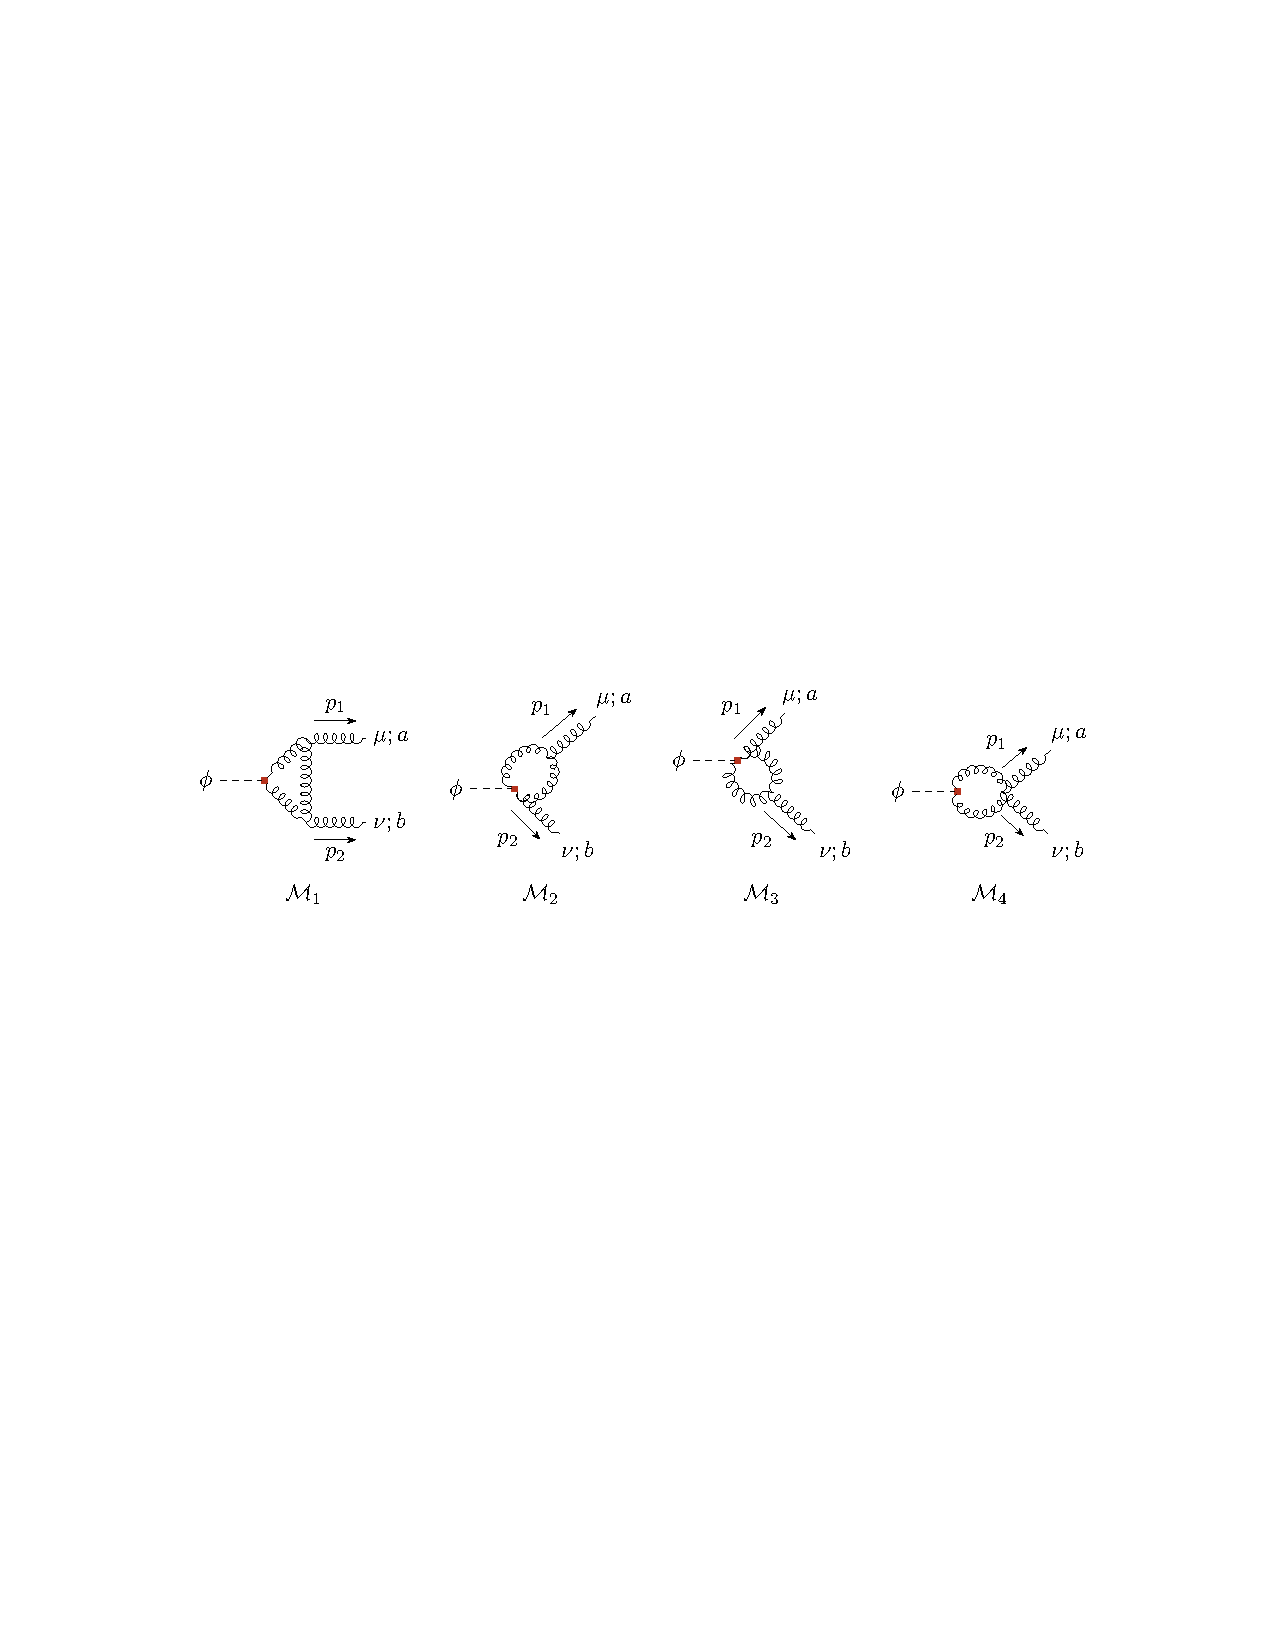
\includegraphics[width = \textwidth]{images/ALP_diagrams_phiGG.pdf}
\caption[Feynman diagrams renormalizing the vertex $\phi GG$]{Feynman diagrams contributing to the renormalization of the vertex $\phi GG$.}
\label{fig:ALPPhiGGdiagB}
\end{figure}

\begin{figure}[h!tb]
\centering
\begin{tikzpicture}
	\begin{feynman}[small]
	\node [BrickRed, square dot] (b);
    \vertex [above left=1.5cm of b] (a) {$\phi$};
    \vertex [below left=0.75cm of b] (c) ;
    \vertex [above right=1.5cm of b] (d) {\(\mu;a\)};
	\vertex [below right =1.5cm of b] (e) {\(\nu;b\)} ;
    \diagram*{
    (a) -- [scalar] (b),
    (b) -- [gluon, momentum=\(p_2\)] (e),
    (b) -- [gluon, momentum=\(p_1\)] (d),
    (b) -- [gluon, half left] (c),
    (c) -- [gluon, half left] (b),
    };
	\end{feynman}
	\end{tikzpicture}
\quad
\begin{tikzpicture}
	\begin{feynman}[small]
	\vertex (a) {\(\phi\)};
	\node [BrickRed, square dot, right=  of a] (b);
	\vertex [above right = of b] (c);
	\vertex [below right=of b] (d);
	\vertex [right =  of c] (e) {\(\mu;a\)} ;
	\vertex [right =  of d] (f) {\(\nu;b\)} ;
	\diagram*{
		(a) -- [scalar] (b),
		(c) -- [fermion] (b),
		(b) -- [fermion] (d),
		(d) -- [gluon, momentum'=\(p_2\)] (f),
		(d) -- [fermion] (c),
		(c) -- [gluon, momentum=\(p_1\)] (e),
	};
	\end{feynman}
	\end{tikzpicture}
    \quad
    \begin{tikzpicture}
	\begin{feynman}[small]
	\vertex (a) {\(\phi\)};
	\node [BrickRed, square dot, right=  of a] (b);
	\vertex [above right = of b] (c);
	\vertex [below right=of b] (d);
	\vertex [right =  of c] (e) {\(\mu;a\)} ;
	\vertex [right =  of d] (f) {\(\nu;b\)} ;
	\diagram*{
		(a) -- [scalar] (b),
		(c) -- [anti fermion] (b),
		(b) -- [anti fermion] (d),
		(d) -- [gluon, momentum'=\(p_2\)] (f),
		(d) -- [anti fermion] (c),
		(c) -- [gluon, momentum=\(p_1\)] (e),
	};
	\end{feynman}
	\end{tikzpicture}
\caption[Feynman diagrams not contributing to the renormalization of the vertex $\phi GG$]{Feynman diagrams that do not contribute to the renormalization of the vertex
$\phi G G$ because they are either identically zero or because they give rise to no UV
divergences.}
\label{fig:ALPPhiGGdiagBNotDiv}
\end{figure}

We find the following divergent terms for the diagrams in Figure~\ref{fig:ALPPhiGGdiagB}:
\begin{align}
    i {\mathcal{M}_{1}}^{ab}_{\mu\nu} &= i \frac{\alpha_s}{3\pi \epsilon} \frac{\mathcal{C}_g}{\Lambda} C_A \delta^{ab}\left[ (23 + 6 \xi_G) p_{1\nu} p_{2 \mu} - (37 + 6 \xi_G) p_1\cdot p_2 g_{\mu\nu}\right]\,,\\
    i {\mathcal{M}_{2}}^{ab}_{\mu\nu} &= i \frac{\alpha_s}{2 \pi \epsilon} \frac{\mathcal{C}_g}{\Lambda} C_A \delta^{ab}(5 +  \xi_G) \left(-p_{1\nu} p_{2 \mu} + p_1\cdot p_2 g_{\mu\nu} \right)\,, \\
    i {\mathcal{M}_{3}}^{ab}_{\mu\nu} &= i \frac{\alpha_s}{2 \pi \epsilon} \frac{\mathcal{C}_g}{\Lambda} C_A \delta^{ab}(5 +  \xi_G) \left(-p_{1\nu} p_{2 \mu} + p_1\cdot p_2 g_{\mu\nu} \right)\,,\\
    i {\mathcal{M}_{4}}^{ab}_{\mu\nu} &=
    i \frac{\alpha_s}{3 \pi \epsilon} \frac{\mathcal{C}_g}{\Lambda} C_A \delta^{ab}\left(p_{1\nu} p_{2 \mu} + 13 p_1\cdot p_2 g_{\mu\nu} \right)
    \,,
\end{align}
which add up to
\begin{equation}
i \mathcal{M}^{ab}_{\mu\nu} = i \frac{\alpha_s}{\pi \epsilon}\frac{\mathcal{C}_g}{\Lambda}C_A \delta^{ab}  (3+ \xi_G) \left(p_{1\nu} p_{2\mu} - p_1 \cdot p_2 g_{\mu\nu}\right)\,,
\end{equation}
where $\xi_G$ is the gluon gauge-fixing parameter.
Therefore, from the Feynman rule for $\phi GG$,
\begin{equation}
    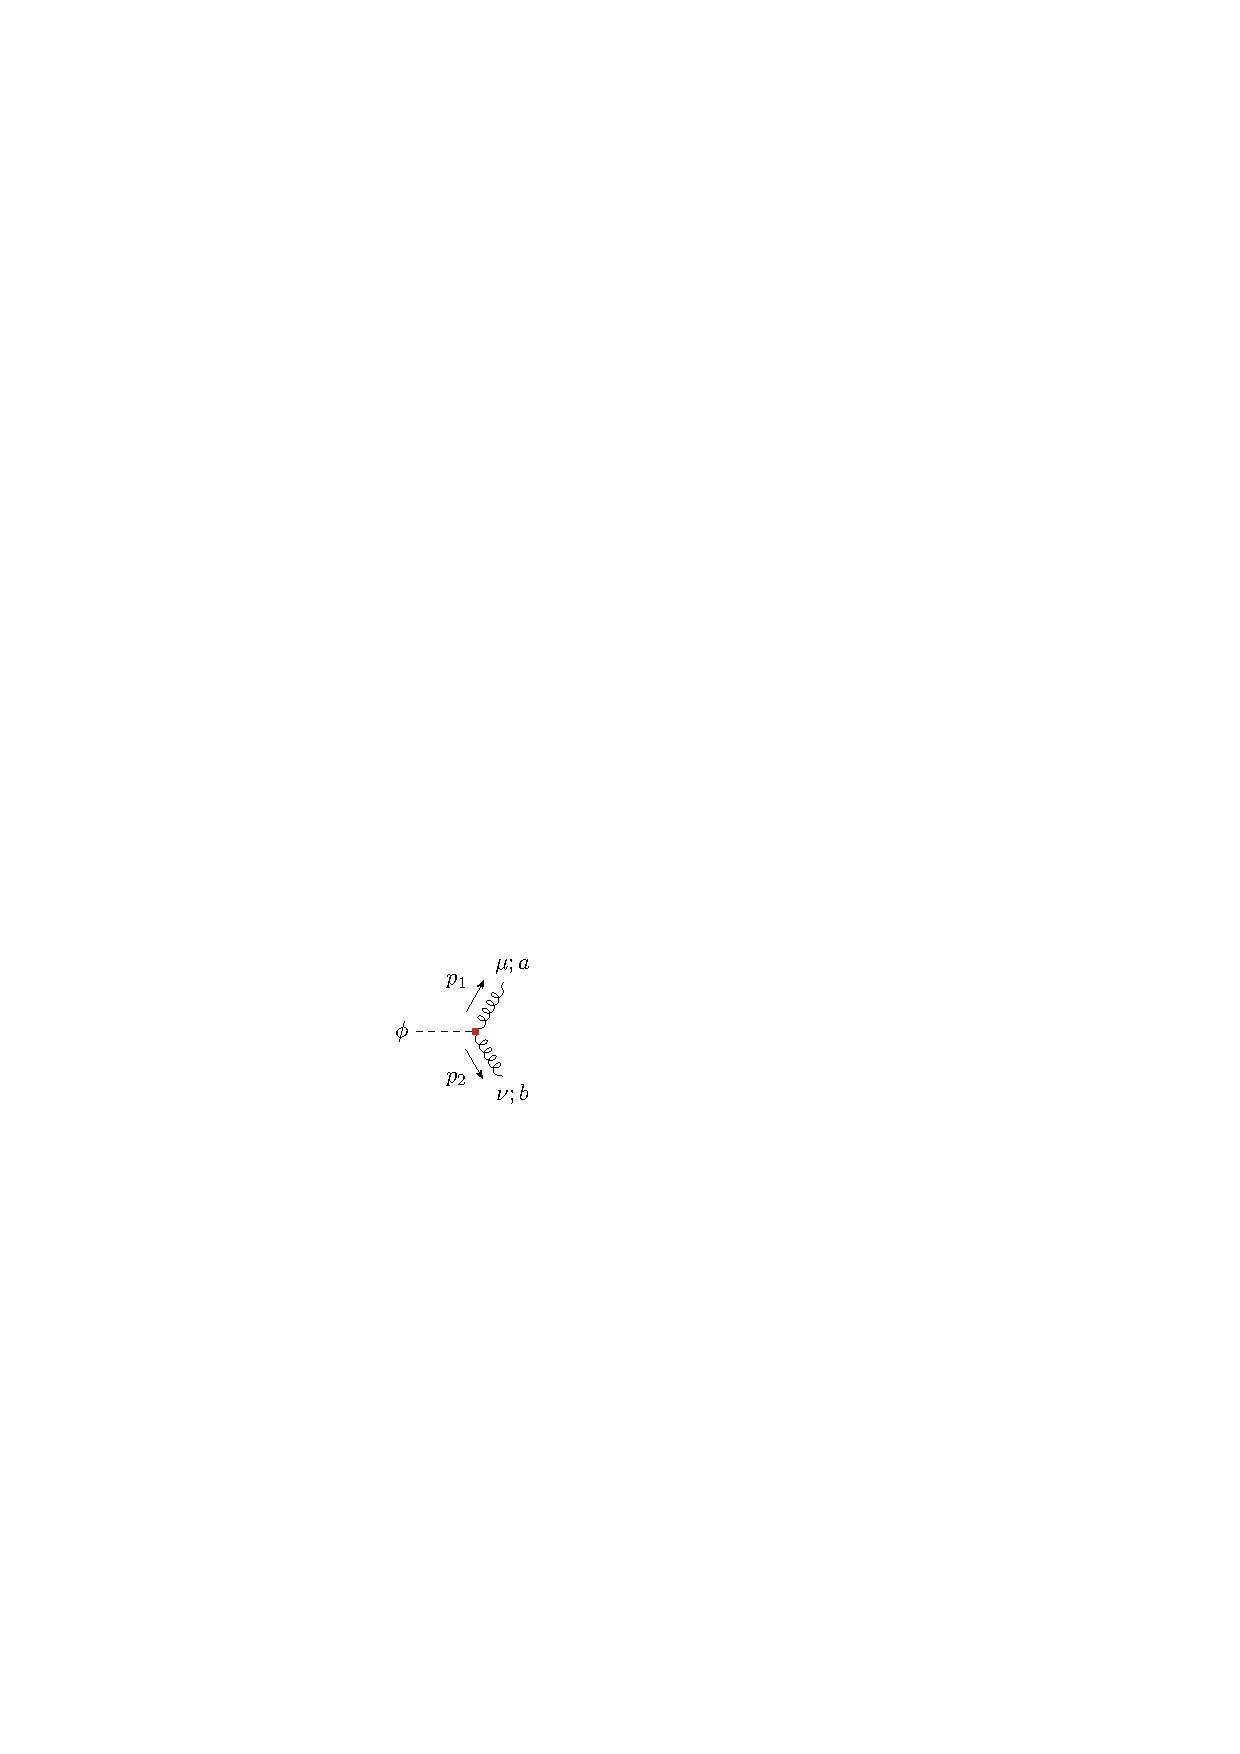
\includegraphics[valign=c,page=1]{images/ALP_FeynRules.pdf}
    = 4i \frac{\mathcal C_g}{\Lambda}\delta^{ab}(p_{1\nu} p_{2\mu} - p_1 \cdot p_2 g_{\mu\nu})\,,
\end{equation}
we can identify the renormalization factor of $\mathcal C_g$ to be
\begin{equation}
     Z_{\mathcal C_g} = 1 - \frac{\alpha_s}{4\pi\epsilon} (3+\xi_G) C_A \,.
\end{equation}
Finally, by exploiting the expression for the renormalization factor of the gluon field,
\begin{equation}
    Z_g =1+ \frac{\alpha_s}{4\pi \epsilon}\bigg[\bigg(\frac{13}{3}-\xi_G\bigg)C_A-\frac{8}{3}T_F \sum_f c_f^2 \bigg]\,,
\end{equation}
and $\mu\dv[]{}{\mu}\alpha_s=-\epsilon \alpha_s + \dotsb$, we obtain the following RGE:
\begin{equation}
    \frac{1}{\mathcal{C}_g} \mu \dv[]{\mathcal C_g}{\mu} =  -  \frac{1}{Z_{\mathcal C_g}} \mu \dv[]{Z_{\mathcal C_g}}{\mu} +  \frac{1}{Z_g} \mu \dv[]{Z_g}{\mu} = - \frac{\alpha_s}{2\pi} \bigg[ \frac{11}{3} C_A - \frac{4}{3}T_F \sum_f c_f^2 \bigg]\,.
\end{equation}
These results reproduce the ones obtained with the on-shell method, but at the expense of
computing a relatively large number of one-loop diagrams with non-trivial Lorentz and
gauge-dependent structures.
In the on-shell method, no gauge dependence is present at any level of the computation, which
requires only the convolution of one tree-level amplitude with a single form factor.

Additionally, the on-shell method allows us to manifest some hidden structures of the
computation which are jeopardized in the standard approach.
Indeed, owing to general symmetry arguments, one would expect the operator $\phi GG$ to
renormalize precisely as $GG$, and, hence, just like the infrared anomalous dimension
associated with a pair of gluons, whose long-distance dynamics is clearly dictated by their
kinetic term.
The on-shell method formalizes this property in a rather elegant way: a simple inspection of
the form of a few tree-level amplitudes directly allows us to solidly derive such a property.

Another interesting example is given by the renormalization of the Weinberg
$GG\widetilde G$ operator.
Its Feynman rule in momentum space is given by
\begin{equation}
    \includegraphics[valign=c,page=2]{images/ALP_FeynRules.pdf}
    \begin{aligned}
    &= -\frac{2}{3}\frac{d_G}{\Lambda^2}f^{abc}[\epsilon_{\mu\nu\rho\alpha}(p_1^\alpha p_2\cdot p_3+p_2^\alpha p_3\cdot p_1+p_3^\alpha p_1\cdot p_2)
    \\
    &+\epsilon_{\mu\nu\alpha\beta}(p_1-p_2)_\rho p_1^\alpha p_2^\beta  + \epsilon_{\nu\rho\alpha\beta}(p_2-p_3)_\mu p_2^\alpha p_3^\beta + \epsilon_{\rho\mu\alpha\beta}(p_3-p_1)_\nu p_3^\alpha p_1^\beta
    ]\,.
    \end{aligned}
\end{equation}
Within the standard diagrammatic framework, extracting its anomalous dimension requires
computing different diagrams, which we can conveniently classify as triangle and bubble
diagrams; see Figure~\ref{fig:ALPWeinbergdiagrams}.

\begin{figure}[h!tb]
\centering
\begin{tikzpicture}
	\begin{feynman}[small]
	\vertex (a) {\(\mu;a\)};
	\node [NavyBlue, square dot, right= 1.5cm of a] (b);
	\node [BrickRed, square dot, above right=of b] (c);
	\vertex [below right=of b] (d);
	\vertex [right=1.7cm of c] (e) {\(\nu;b\)} ;
	\vertex [right=1.3cm of d] (f) {\(\rho;c\)} ;
	\vertex (g) [below =of a] {\(\mathcal{M}_{1}^\triangle\)};
	\diagram*{
		(a) -- [gluon, rmomentum=\(p_1\)] (b),
		(c) -- [scalar] (b),
		(b) -- [gluon] (d),
		(d) -- [gluon, momentum'=\(p_3\)] (f),
		(d) -- [gluon] (c),
		(c) -- [gluon, momentum=\(p_2\)] (e),
	};
	\end{feynman}
	\end{tikzpicture}
\qquad
\begin{tikzpicture}
	\begin{feynman}[small]
	\vertex (a) {\(\mu;a\)};
	\node [BrickRed, square dot, right= 1.5cm of a] (b);
	\node [NavyBlue, square dot, above right=of b] (c);
	\vertex [below right=of b] (d);
	\vertex [right=1.7cm of c] (e) {\(\nu;b\)} ;
	\vertex [right=1.3cm of d] (f) {\(\rho;c\)} ;
	\vertex (g) [below =of a] {\(\mathcal{M}_{2}^\triangle\)};
	\diagram*{
		(a) -- [gluon, rmomentum=\(p_1\)] (b),
		(c) -- [scalar] (b),
		(b) -- [gluon] (d),
		(d) -- [gluon, momentum'=\(p_3\)] (f),
		(d) -- [gluon] (c),
		(c) -- [gluon, momentum=\(p_2\)] (e),
	};
	\end{feynman}
	\end{tikzpicture}
    \\
    \begin{tikzpicture}[baseline = (aux)]
	\begin{feynman}[small]
	\vertex (a) {\(\mu;a\)};
    \vertex [above =0.7cm of a] (aux)  ;
	\node [NavyBlue, square dot, right=1.5cm of a] (b);
	\node [BrickRed, square dot,  right=1.3 cm of b] (c);
	\vertex [above right=1.5cm of c] (e) {\(\nu;b\)} ;
	\vertex [below right=1.5cm of c] (f) {\(\rho;c\)} ;
	\vertex (g) [below = of a] {\(\mathcal{M}_{1}^\bigcirc\)};
	\diagram*{
		(a) -- [gluon, rmomentum=\(p_1\)] (b),
		(c) -- [scalar, half left] (b),
		(b) -- [gluon, half left] (c),
		(c) -- [gluon, momentum'=\(p_3\)] (f),
		(c) -- [gluon, momentum'=\(p_2\)] (e),
	};
	\end{feynman}
	\end{tikzpicture}
    \qquad
    \begin{tikzpicture}[baseline = (aux)]
	\begin{feynman}[small]
	\vertex (a) {\(\mu;a\)};
    \vertex [above =0.7cm of a] (aux)  ;
	\node [BrickRed, square dot, right=1.5cm of a] (b);
	\node [NavyBlue, square dot,  right=1.3 cm of b] (c);
	\vertex [above right=1.5cm of c] (e) {\(\nu;b\)} ;
	\vertex [below right=1.5cm of c] (f) {\(\rho;c\)} ;
	\vertex (g) [below = of a] {\(\mathcal{M}_{2}^\bigcirc\)};
	\diagram*{
		(a) -- [gluon, rmomentum=\(p_1\)] (b),
		(c) -- [scalar, half left] (b),
		(b) -- [gluon, half left] (c),
		(c) -- [gluon, momentum'=\(p_3\)] (f),
		(c) -- [gluon, momentum'=\(p_2\)] (e),
	};
	\end{feynman}
	\end{tikzpicture}
\caption[Feynman diagrams renormalizing the three-gluon Weinberg operator]{Triangle and bubble diagrams contributing to the renormalization of the three-gluon
Weinberg operator. The eight additional amplitudes with the three external gluons permuted are
omitted.}
\label{fig:ALPWeinbergdiagrams}
\end{figure}

The divergences associated with the first class of three-point diagrams are, with
$d=4-\epsilon$,
\begin{align}
    i {\mathcal M_{1}^\triangle}_{\mu\nu\rho}^{abc} &= \frac{1}{\epsilon}\frac{\mathcal C_g \widetilde{\mathcal C}_g}{3\pi^2 \Lambda^2}g_sf^{abc}\big[-\epsilon_{\mu\nu\rho\alpha}(p_1\cdot p_2+5p_2\cdot p_3)p_1^\alpha
    +\epsilon_{\mu\nu\alpha\beta}(2p_1+p_3)_\rho p_1^\alpha p_2^\beta \nonumber \\
    &\quad
    -4 \epsilon_{\mu\nu\alpha\beta}p_{2\rho} p_1^\alpha p_3^\beta
    + \epsilon_{\mu\rho\alpha\beta}(p_1+5p_3)_\nu p_1^\alpha p_2^\beta - 4 g_{\nu\rho}\epsilon_{\mu\alpha\beta\gamma}p_1^\alpha p_2^\beta p_3^\gamma
    \big]\,,\\
    i {\mathcal M_{2}^\triangle}_{\mu\nu\rho}^{abc} &= \frac{1}{\epsilon}\frac{\mathcal C_g \widetilde{\mathcal C}_g}{3\pi^2 \Lambda^2}g_sf^{abc}\big[
    \epsilon_{\mu\nu\rho\alpha}p_1^2 p_2^\alpha
    -4 \epsilon_{\mu\nu\rho\alpha}p_2^\alpha  p_1\cdot p_3
    + \epsilon_{\mu\nu\alpha\beta}(3p_1+p_3)_\rho p_1^\alpha p_2^\beta \nonumber \\
    &\quad
    - 5 \epsilon_{\mu\nu\alpha\beta}p_{1\rho} p_2^\alpha p_3^\beta
    +\epsilon_{\nu\rho\alpha\beta}(4p_3-p_1)_\mu p_1^\alpha p_2^\beta
    -5 g_{\mu\rho} \epsilon_{\nu\alpha\beta\gamma} p_1^\alpha p_2^\beta p_3^\gamma
    \big]\,.
\end{align}
By taking into account the permutations of the three external gluons, the sum of these diagrams
amounts to
\begin{equation}
i {\mathcal{M}^{\triangle}}_{\mu\nu\rho}^{abc} = \frac{1}{\epsilon}\frac{2\mathcal C_g \widetilde{\mathcal C}_g}{\pi^2 \Lambda^2}g_s f^{abc} \big[
2\epsilon_{\mu\nu\alpha\beta}p_{2\rho}
+ 2\epsilon_{\mu\rho\alpha\beta}p_{3\nu}
+\epsilon_{\nu\rho\alpha\beta}(p_3-p_2)_\mu
\big] p_2^\alpha p_3^\beta\,,
\end{equation}
where we assumed energy-momentum conservation $p_1 = - (p_2+p_3)$, the transversality
conditions for gluons, and $p_2^2=p_3^2=p_2\cdot p_3 = 0$.
The divergences associated with the two-point diagrams read instead
\begin{align}
    i {\mathcal M_{1}^\bigcirc}_{\mu\nu\rho}^{abc} &= -\frac{1}{\epsilon}\frac{\mathcal C_g \widetilde{\mathcal C}_g}{3\pi^2\Lambda^2}g_sf^{abc}(3m_\phi^2 -p_1^2)\epsilon_{\mu\nu\rho\alpha}p_1^\alpha \,,
    \\
    i {\mathcal M_{2}^\bigcirc}_{\mu\nu\rho}^{abc} &= -\frac{1}{\epsilon}\frac{\mathcal C_g \widetilde{\mathcal C}_g}{3\pi^2\Lambda^2}g_sf^{abc}
    \big[
    \epsilon_{\mu\nu\rho\alpha}[(3m_\phi^2+p_1^2)p_1^\alpha
    +3p_1^2 (p_2+p_3)^\alpha ]\nonumber \\
    &\quad -3\epsilon_{\nu\rho\alpha\beta}p_{1\mu}p_1^\alpha(p_2+p_3)^\beta
    \big]\,,
\end{align}
which are not of the desired form of the Feynman rule of $GG\widetilde G$ and can only be
interpreted as pertaining to the renormalization of the $G\widetilde G$ operator.
Indeed, the Feynman rule of the $G\widetilde G$ operator is proportional to $p_1+p_2+p_3$,
which has to vanish for on-shell gluons, as is indeed the case for these bubble contributions.
Moreover, we find that tadpole diagrams are identically vanishing.
As a consequence, the RGE associated with the Wilson coefficient $d_G$ is
\begin{equation}
    \mu\dv[]{}{\mu}d_G = -\frac{3g_s}{\pi^2}\mathcal C_g \widetilde{\mathcal C}_g\,.
\end{equation}
This reproduces the result previously reported in Eq.~\eqref{eq:ALPgammatildeG3}, but at the
price of computing more diagrams with different Lorentz structures.
On the other hand, the on-shell method only required the calculation of one form factor and one
amplitude, yielding the same result in a more transparent and elegant way.

Yet another advantage of the on-shell method is that it directly allows us to relate the
anomalous dimension for a given operator to the one of its CP counterpart, such as $\phi FF$ to
$\phi F \widetilde F$ or
$\phi \bar f f$ to $\phi \bar f i \gamma_5 f$.
In the previous example, for instance, the knowledge of the anomalous dimension for the
operator $\phi GG$ allowed us to immediately infer the one for the operator
$\phi G\widetilde G$, see Section~\ref{sec:ALPphiGG}, and similarly for $GGG$ and
$GG \widetilde{G}$, see Section~\ref{sec:ALPGGG}.
Such a duality is not manifest when working in the standard approach, where CP-dual operators
possess entirely different Lorentz structures at the level of Feynman rules, and no similarity
in the pattern of cancellations among gauge-dependent terms is present, despite the common
diagrammatic structure.

\section{Conclusions}
\label{sec:ALPconclusions}

On-shell amplitude techniques have proven to be very effective for computing the RGEs of quantum field theories~\cite{Caron-Huot:2016cwu,EliasMiro:2020tdv,Baratella:2020lzz,Jiang:2020mhe,Bern:2020ikv,Baratella:2020dvw,AccettulliHuber:2021uoa,EliasMiro:2021jgu,Baratella:2022nog,Machado:2022ozb}. 
In particular, the on-shell method~\cite{Caron-Huot:2016cwu} relates anomalous dimensions to unitarity cuts. 
As discussed in Chapter~\ref{ch:RGEmethod}, this method can also be easily applied to describe mixings among operators with different dimensions 
and to capture leading mass effects, which are of paramount importance in several phenomenological studies.

In this chapter, we have extensively applied the above techniques~\cite{Caron-Huot:2016cwu,Bresciani:2023jsu} to the one-loop renormalization of CP-violating interactions, both above and below the electroweak scale,  of an ALP with SM fields, reproducing and extending previous results~\cite{Marciano:2016yhf,DiLuzio:2020oah,Bauer:2020jbp,Chala:2020wvs,DasBakshi:2023lca,Galda:2021hbr,Galda:2023qjx}.

In particular, we  first derived the anomalous dimensions for ALP couplings with fermions, $\phi \bar f f$ and $\phi \bar f i \gamma_5 f$, which require a fermion mass insertion. This allowed us to apply the on-shell method~\cite{Caron-Huot:2016cwu} supplemented by the Higgs low-energy theorem to keep track of leading mass effects while still working in a massless formalism~\cite{Bresciani:2023jsu}. 

Then, we considered the renormalization of ALP couplings to photons and gluons, $\phi FF$ and $\phi GG$, along with their CP counterparts, $\phi F \tildee F$ and $\phi G \tildee G$, recovering the well-known result that they renormalize precisely as $FF$ and $GG$ and, hence, just like their related gauge couplings squared. 
The on-shell method shows this property in a simple and elegant way by just inspecting a few tree-level amplitudes.
Moreover, we evaluated the RGEs of operators up to dimension-six emerging after integrating out the ALP at one-loop level,  
such as the Weinberg operator $GG\tildee G$ and $GGG$, the (chromo-)magnetic and (chromo-)electric dipole moments, 
i.e., $\bar f \sigma\!\cdot\! F f$, $\bar f \sigma\!\cdot\! G f$,
$\bar f \sigma\!\cdot\! F i\gamma_5 f$, and $\bar f \sigma\!\cdot\! G i\gamma_5 f$.

A detailed derivation of the anomalous-dimension matrix was carried out both with on-shell and standard techniques, 
aiming to closely compare their virtues and shortcomings.
%
We found that on-shell methods are computationally advantageous compared to standard ones, owing to the
significantly lower and less challenging number of required contributions to be computed.
Moreover, the presence of a large number of non-Abelian gauge bosons generally renders calculations with standard techniques lengthy and computationally expensive: checks for gauge invariance were performed, often involving non-trivial cancellation of different Lorentz and gauge structures.

Remarkably, the on-shell method makes more manifest the connection between the anomalous dimension of operators related by symmetries. 
For instance, the knowledge of the anomalous dimension for the operator $\phi GG$ allowed us to immediately 
infer the one for the CP-dual operator $\phi G\tildee G$: this duality is hidden within the standard approach, where CP-dual operators have different Lorentz structures at the level of Feynman rules, and no similarity in the pattern of cancellations among gauge-dependent terms is present.

Our results were obtained by systematically evaluating all phase-space cut integrals adopting two different integration techniques, namely by angular integration~\cite{Zwiebel:2011bx} and via Stokes' theorem~\cite{Mastrolia:2009dr}. The latter, motivated by unitarity, offers the advantage of projecting directly the rational coefficient of the two-point functions out of the double cut of one-loop integrals, therefore simplifying the evaluation of anomalous dimensions.  
It would be interesting to extend Stokes integration method for the evaluation of multi-particle phase-space integrals and to apply it for the evaluation of anomalous dimensions at higher orders by unitarity cuts, which we plan for future developments.

\begin{subappendices}

%%%%%%%%%%%%%%%%%%%%%%%%%%%
\section{Amplitudes}
\label{app:ALP_amplitudes_RGE}
%%%%%%%%%%%%%%%%%%%%%%%%%%%

In this appendix, we report the amplitudes that we employed throughout the chapter, expressed
in terms of spinor-helicity variables.

\subsection{Three-Point Tree Amplitudes}

Here, the analytically continued three-point tree amplitudes in the holomorphic ($\mathsf{H}$)
and anti-holomorphic ($\mathsf{A}$) configurations, belonging to the different sectors of the
Lagrangian, are displayed on the left and on the right, respectively.
As discussed in Section~\ref{sec:3pointamplitudes}, they are completely constrained, up to an overall factor given by the coupling constant, by
locality, Poincaré invariance, and dimensional analysis~\cite{Benincasa:2007xk}.
Indeed, in full generality they read as follows:
\begin{align}
    \mathcal M_3^\mathsf{H}(1^{h_1},2^{h_2},3^{h_3}) = g_\mathsf{H} \agl{1}{2}^{a_3}\agl{2}{3}^{a_1}\agl{3}{1}^{a_2}\,, &&
    \mathcal M_3^\mathsf{A}(1^{h_1},2^{h_2},3^{h_3}) = g_\mathsf{A} \sqr{1}{2}^{\overline a_3}\sqr{2}{3}^{\overline a_1}\sqr{3}{1}^{\overline a_2}\,,
\end{align}
with $\overline a_i=-a_i$,
\begin{align}
    a_1= h_1-h_2-h_3\,,&&
    a_2= h_2-h_3-h_1\,, &&
    a_3= h_3-h_1-h_2\,,
\end{align}
and the mass dimensions of the coupling constants only depend on the helicities:
\begin{align}
    [g_\mathsf{H}]=1+h_1+h_2+h_3\,, &&
    [g_\mathsf{A}]=1-h_1-h_2-h_3\,.
\end{align}
Locality implies that the non-vanishing coupling has $[g]\le 1$. Therefore, 
the consistent configuration is determined by the sign of the sum of the helicities: three-point amplitudes have support on the holomorphic (anti-holomorphic) one if $h_1+h_2+h_3<0$ ($h_1+h_2+h_3>0$).
The case in which $h_1+h_2+h_3=0$ is trivial, as it can only correspond to a cubic scalar
interaction, where $h_1=h_2=h_3=0$.

\paragraph{\texorpdfstring{$\mathcal L_{\text{LO}}$}{L LO}.}
The lowest-order Lagrangian
\begin{equation}
    \mathcal L_{\text{LO}} = -\frac{1}{4}G_{\mu\nu}^a G^{a\mu\nu}-\frac{1}{4}F_{\mu\nu}F^{\mu\nu}+i\bar f_i \gamma^\mu D_\mu f_i - y_i h \bar f_i f_i
\end{equation}
generates
\begin{align}
    \mathcal M(1^-_{f_i},2^+_{\bar f_j},3^-_\gamma) &= \sqrt 2 e Q_f \delta^{ij} \frac{\agl{1}{3}^2}{\agl{1}{2}}\,, &
     \mathcal M(1^-_{f_i},2^+_{\bar f_j},3^+_\gamma) &= \sqrt 2 e Q_f \delta^{ij}\frac{\sqr{3}{2}^2}{\sqr{1}{2}}\,, \\
     \mathcal M(1^-_{f_i^I},2^+_{\bar f_j^J},3^-_{g^a}) &= \sqrt 2 g_s c_f T^a_{IJ}\delta^{ij} \frac{\agl{1}{3}^2}{\agl{1}{2}}\,, &
     \mathcal M(1^-_{f_i^I},2^+_{\bar f_j^J},3^+_{g^a}) &= \sqrt 2 g_s c_f T^a_{IJ} \delta^{ij}\frac{\sqr{3}{2}^2}{\sqr{1}{2}}\,, \\
     \mathcal M(1^-_{g^a},2^-_{g^b},3^+_{g^c}) &= i\sqrt 2 g_s f^{abc}\frac{\agl{1}{2}^3}{\agl{1}{3}\agl{3}{2}}\,,  &
     \mathcal M(1^+_{g^a},2^+_{g^b},3^-_{g^c}) &=-i\sqrt 2 g_s f^{abc}\frac{\sqr{1}{2}^3}{\sqr{1}{3}\sqr{3}{2}}\,,  \\
     \mathcal M(1^-_{f_i},2^-_{\bar f_j},3_h) &= - y_i\delta^{ij}\agl{1}{2}\,, &
     \mathcal M(1^+_{f_i},2^+_{\bar f_j},3_h) &= - y_i \delta^{ij} \sqr{1}{2} \,.
\end{align}

\paragraph{\texorpdfstring{$\mathcal L_{\phi}$}{L phi}.}
The ALP effective Lagrangian
\begin{equation}
    \mathcal{L}_\phi =
    \frac{\widetilde{\mathcal{C}}_\gamma}{\Lambda}\,\phi\, F\widetilde F
    + \frac{\widetilde{\mathcal{C}}_g}{\Lambda}\,\phi\, G\widetilde G
    + \mathcal{Y}^{ij}_P\,\phi\, \bar{f}_i i\gamma_5 f_j
     + \frac{\mathcal{C}_\gamma}{\Lambda}\,\phi\, FF
    + \frac{\mathcal{C}_g}{\Lambda}\,\phi\, GG
    + \mathcal{Y}^{ij}_S\,\phi\, \bar{f}_i f_j
\end{equation}
generates
\begin{align}
    \mathcal M(1^-_\gamma,2^-_\gamma,3_\phi) &= -\frac{2}{\Lambda}(\mathcal C_\gamma + i \widetilde{\mathcal{C}}_\gamma)\agl{1}{2}^2\,, &
    \mathcal M(1^+_\gamma,2^+_\gamma,3_\phi) &= -\frac{2}{\Lambda}(\mathcal C_\gamma - i \widetilde{\mathcal{C}}_\gamma)\sqr{1}{2}^2\,, \\
    \mathcal M(1^-_{g^a},2^-_{g^b},3_\phi) &= -\frac{2}{\Lambda}(\mathcal C_g + i \widetilde{\mathcal{C}}_g)\delta^{ab}\agl{1}{2}^2\,, &
    \mathcal M(1^+_{g^a},2^+_{g^b},3_\phi) &= -\frac{2}{\Lambda}(\mathcal C_g - i \widetilde{\mathcal{C}}_g)\delta^{ab}\sqr{1}{2}^2\,, \\
    \mathcal M(1^-_{f_i},2^-_{\bar f_j},3_\phi)&=(\mathcal Y_S^{ij}-i\mathcal Y_P^{ij})\agl{1}{2}\,, &
    \mathcal M(1^+_{f_i},2^+_{\bar f_j},3_\phi)&=(\mathcal Y_S^{ij}+i\mathcal Y_P^{ij})\sqr{1}{2} \,.
\end{align}

\paragraph{\texorpdfstring{$\mathcal L^{(5)}$}{L(5)}.}
The relevant dimension-five Lagrangian invariant under $SU(3)_c\times U(1)_{\text{em}}$ and
built of SM particles consists of dipole operators,
\begin{equation}
    \mathcal L^{(5)} = \frac{c_{\text{M}}^{ij}}{\Lambda}\bar f_i \sigma^{\mu\nu} f_j F_{\mu\nu} + \frac{c_{\text{E}}^{ij}}{\Lambda}\bar f_i \sigma^{\mu\nu}i\gamma_5 f_j F_{\mu\nu} + \frac{c_{\text{CM}}^{ij}}{\Lambda}\bar f_i \sigma^{\mu\nu}T^a f_j G^a_{\mu\nu} + \frac{c_{\text{CE}}^{ij}}{\Lambda}\bar f_i \sigma^{\mu\nu}i\gamma_5 T^a f_j G^a_{\mu\nu}\,,
\end{equation}
and generates
\begin{align}
    \mathcal M(1^-_{f_i},2^-_{\bar f_j},3^-_\gamma) &= \frac{2\sqrt 2}{\Lambda}C_\gamma^{ij}\agl{1}{3}\agl{2}{3}\,, &
    \mathcal M(1^+_{f_i},2^+_{\bar f_j},3^+_\gamma)&=- \frac{2\sqrt 2}{\Lambda}(C_\gamma^{ij})^*\sqr{1}{3}\sqr{2}{3}\,,  \\
    \mathcal M(1^-_{f_i^I},2^-_{\bar f_j^J},3^-_{g^a}) &= \frac{2\sqrt 2}{\Lambda}C_g^{ij}T^a_{IJ}\agl{1}{3}\agl{2}{3}\,, &
    \mathcal M(1^+_{f_i^I},2^+_{\bar f_j^J},3^+_{g^a})&= - \frac{2\sqrt 2}{\Lambda}(C_g^{ij})^*T^a_{IJ}\sqr{1}{3}\sqr{2}{3}\,,
\end{align}
with
\begin{align}
    C_\gamma^{ij}=c_{\text{M}}^{ij}-i\, c_{\text{E}}^{ij}\,, && C_g^{ij}=c_{\text{CM}}^{ij}-i\,c_{\text{CE}}^{ij}\,.
\end{align}

\paragraph{\texorpdfstring{$\mathcal L^{(6)}$}{L(6)}.}
The relevant dimension-six Lagrangian invariant under $SU(3)_c\times U(1)_{\text{em}}$ and built
of SM particles only consists of
\begin{equation}
    \mathcal L^{(6)} = \frac{D_G}{3\Lambda^2} f^{abc} G_\mu^{a, \nu} G_{\nu}^{b, \rho} G_{\rho}^{c, \mu} + \frac{d_G}{3\Lambda^2} f^{abc} G_\mu^{a, \nu} G_{\nu}^{b, \rho} \widetilde G_{\rho}^{c, \mu}
\end{equation}
and generates
\begin{align}
    \mathcal M(1^-_{g^a},2^-_{g^b},3^-_{g^c}) = i\frac{\sqrt 2}{\Lambda^2}C_Gf^{abc}\agl{1}{2}\agl{2}{3}\agl{1}{3}\,, &&
     \mathcal M(1^+_{g^a},2^+_{g^b},3^+_{g^c}) = i\frac{\sqrt 2}{\Lambda^2}C_G^* f^{abc}\sqr{2}{1}\sqr{3}{2}\sqr{3}{1}\,,
\end{align}
with
\begin{equation}
    C_G= D_G + i\, d_G\,.
\end{equation}

\subsection{Four-Point Tree Amplitudes}

Here, the four-point tree amplitudes needed for the calculations are displayed.
With the symbol $*$ we denote the region in the space of the couplings of the theory where only
the gauge couplings $e$ and $g_s$ are different from zero.
\begin{align}
     \mathcal M|_*(1^-_{f_i},2^+_{\bar f_j},3^-_\gamma,4^+_\gamma) &= -2e^2Q_f^2\delta^{ij}\frac{\agl{1}{3}\sqr{4}{2}}{\agl{1}{4}\sqr{3}{1}}\,, \\
    \mathcal M|_*(1^+_{f_i},2^-_{\bar f_j},3^-_\gamma,4^+_\gamma) &= -2e^2Q_f^2\delta^{ij}\frac{\agl{2}{3}\sqr{4}{1}}{\agl{1}{4}\sqr{3}{1}}\,, \\
    \mathcal M|_*(1^-_{f_i^I},2^+_{\bar f_j^J},3^-_{g^a},4^+_{g^b}) &= -2g_s^2c_f^2T^a_{IK}T^b_{KJ}\delta^{ij}\frac{\agl{1}{3}\sqr{4}{2}}{\agl{1}{4}\sqr{3}{1}}\,, \\
    \mathcal M|_*(1^+_{f_i^I},2^-_{\bar f_j^J},3^-_{g^a},4^+_{g^b}) &= -2g_s^2c_f^2T^b_{IK}T^a_{KJ}\delta^{ij}\frac{\agl{2}{3}\sqr{4}{1}}{\agl{1}{4}\sqr{3}{1}}\,, \\
    \mathcal M|_*(1^-_{g^a},2^-_{g^b},3^+_{g^c},4^+_{g^d}) &= -2g_s^2\agl{1}{2}^4\bigg(\frac{f^{abe}f^{cde}}{\agl{1}{2}\agl{2}{3}\agl{3}{4}\agl{4}{1}}+\frac{f^{ace}f^{bde}}{\agl{1}{3}\agl{3}{2}\agl{2}{4}\agl{4}{1}}\bigg)\,,\\
    \mathcal M|_*(1^-_{f_i^I},2^-_{\bar f_j^J},3^+_{f_k^K},4^+_{\bar f_l^L}) &= -2 (e^2 Q_f^2 \delta_{IL}\delta_{KJ}+g_s^2c_f^2T^a_{IL}T^a_{KJ}) \delta^{il}\delta^{jk} \frac{\agl{1}{2}\sqr{4}{3}}{\agl{1}{4}\sqr{4}{1}}\,, \\
    \mathcal M|_*(1^-_{f_i^I},2^+_{\bar f_j^J},3^-_{f_k^K},4^+_{\bar f_l^L}) &= +2(e^2Q_f^2\delta_{IJ}\delta_{KL}+g_s^2c_f^2T^a_{IJ}T^a_{KL})\delta^{ij}\delta^{kl} \frac{\agl{1}{3}\sqr{4}{2}}{\agl{1}{2}\sqr{2}{1}}\nonumber \\
    &\quad - 2(e^2Q_f^2\delta_{IL}\delta_{KJ}+g_s^2c_f^2T^a_{IL}T^a_{KJ}) \delta^{il}\delta^{jk} \frac{\agl{1}{3}\sqr{4}{2}}{\agl{1}{4}\sqr{4}{1}}\,, \\
    \mathcal M|_*(1^-_{f_i^I},2^+_{\bar f_j^J},3^+_{f_k^K},4^-_{\bar f_l^L}) &= +2(e^2Q_f^2\delta_{IJ}\delta_{KL}+g_s^2c_f^2T^a_{IJ}T^a_{KL})\delta^{ij}\delta^{kl} \frac{\agl{1}{4}\sqr{3}{2}}{\agl{1}{2}\sqr{2}{1}}\,,\\
    \mathcal M(1^-_{f_i},2^+_\gamma,3^-_{\bar f_j},4_h) &= -\sqrt{2} y_i \delta^{ij} e Q_f \frac{\agl{1}{3}^2}{\agl{1}{2}\agl{2}{3}}\,, \\
    \mathcal M(1^-_{f_i^I},2^+_{g^a},3^-_{\bar f_j^J},4_h) &= -\sqrt{2} y_i \delta^{ij} g_s c_f T^a_{IJ} \frac{\agl{1}{3}^2}{\agl{1}{2}\agl{2}{3}} \,,\\
    \mathcal M(1^-_{f_i},2^-_\gamma,3^+_{\bar f_j},4_\phi) &= \frac{2\sqrt 2}{\Lambda} e Q_f \delta^{ij}(\mathcal C_\gamma + i\widetilde{\mathcal C}_\gamma)\frac{\agl{1}{2}^2}{\agl{1}{3}}\,,\\
    \mathcal M(1^-_{f_i^I},2^-_{g^a},3^+_{\bar f_j^J},4_\phi) &= \frac{2\sqrt 2}{\Lambda} g_s c_f T^a_{IJ} \delta^{ij}(\mathcal C_g + i\widetilde{\mathcal C}_g)\frac{\agl{1}{2}^2}{\agl{1}{3}}\,,\\
    \mathcal M(1^-_{f_i},2^-_{\bar f_j},3^+_\gamma,4_\phi) &= -\sqrt 2 e Q_f (\mathcal Y_S^{ij}-i\mathcal Y_P^{ij})\frac{\agl{1}{2}^2}{\agl{1}{3}\agl{2}{3}} \,,\\
    \mathcal M(1^-_{f_i^I},2^-_{\bar f_j^J},3^+_{g^a},4_\phi) &= -\sqrt 2 g_s c_f T^a_{IJ} (\mathcal Y_S^{ij}-i\mathcal Y_P^{ij})\frac{\agl{1}{2}^2}{\agl{1}{3}\agl{2}{3}}\,,\\
    \mathcal M(1^-_{g^a},2^-_{g^b},3^+_{g^c},4_\phi) &= -i\frac{2\sqrt 2}{\Lambda}g_sf^{abc}(\mathcal C_g+i\widetilde{\mathcal C}_g)\frac{\agl{1}{2}^3}{\agl{1}{3}\agl{2}{3}}\,.
\end{align}

%%%%%%%%%%%%%%%%%%%%%%%%%%%
\section{Infrared Anomalous Dimensions}
\label{app:ALP_IR}
%%%%%%%%%%%%%%%%%%%%%%%%%%%

The on-shell method is not directly sensitive to the UV anomalous dimension associated
with a certain operator, $\gamma_{i\leftarrow j}$, but rather to the difference between it and
the infrared anomalous-dimension matrix, $\delta_{ij} \gamma_{i,\text{IR}}$.
Its knowledge is a necessary ingredient for the method, and therefore it is of paramount
importance to understand how to treat it properly.

There are two main approaches to infrared divergences within the scope of the on-shell method.
The first one consists in taking the infrared anomalous dimensions to be external inputs from
other computations.
For instance, at one-loop level the infrared anomalous dimension can be parameterized, in any
gauge theory, as
\begin{equation}
    \gamma_{\text{IR}} (\{p_i\}, \mu) = \frac{g^2}{4 \pi^2} \sum_{i<j} T^a_{ik} T^a_{kj} \log \frac{\mu^2}{-s_{ij}} + \sum_i \gamma_i^{\text{coll.}}\,,
\end{equation}
where $T_{ik}^a$ are the gauge-group generators acting on the particle $i$~\cite{Becher:2009cu}.
The first term of the infrared anomalous dimension stems from soft wide-angle infrared
radiation, whereas the second one describes the effects arising from hard, collinear
divergences.

Alternatively, one can compute the infrared anomalous dimensions via on-shell
techniques~\cite{Caron-Huot:2016cwu}.
Indeed, infrared divergences do not depend specifically on the gauge-invariant operator
appearing within the definition of a form factor, but only on its external states.
As a consequence, one can compute these quantities by simply considering a local,
gauge-invariant operator with a vanishing UV anomalous dimension and allowing for
two-particle interactions.
In this respect, a natural candidate is given by the energy-momentum tensor $T_{\mu\nu}$.
Since the energy-momentum tensor has to be conserved also at the quantum level, its UV
anomalous dimension has to vanish, i.e., $\gamma_{T} = 0$, and we are left with
\begin{equation}
- \gamma_{\text{IR}} \, F_T = D \, F_T\,,
\end{equation}
which implies
\begin{equation}
\label{eq:ALPMaster_Formula_LO}
    \gamma_{\text{IR}} = -\frac{D \, F_T}{F_T} = \frac{1}{\pi} \frac{(\mathcal M F_T) }{F_T}\,.
\end{equation}

In this appendix, we make use of the on-shell method to compute the infrared collinear
anomalous dimensions associated with the external particle states related to those operators
we have considered within the main text.

\subsection{\texorpdfstring{$\phi \bar f f$ and $\phi \bar f i \gamma_5 f$ Operators}{phi fbar f and phi fbar i gamma5 f Operators}}
\label{sec:ALPIRphiffb}

The infrared anomalous dimension $\gamma_{S,\text{IR}}$ associated with the operators
$\phi\, \bar f_i f_j$ and $\phi\, \bar f_i i \gamma_5 f_j$ can be computed through the
master formula
\begin{equation}
    \gamma_{S,\text{IR}} F_T^{\alpha\beta\dot\alpha\dot\beta}|_{*}(1^-_{f_i^I},2^+_{\bar f_j^J})=\frac{1}{\pi}(\mathcal M F_T^{\alpha\beta\dot\alpha\dot\beta})|_{*}(1^-_{f_i^I},2^+_{\bar f_j^J})\,,
\end{equation}
which diagrammatically reads as in Figure~\ref{fig:ALPphiffIR}.

\begin{figure}[h!tb]
\centering
\includegraphics[width=\textwidth,page=13]{images/ALP_diagrams.pdf}
\caption[Diagrammatic formula for computing $\gamma_{S,\text{IR}}$]{Diagrammatic formula for computing $\gamma_{S,\text{IR}}$.}
\label{fig:ALPphiffIR}
\end{figure}

On the left-hand side, we have the form factor of the fermion stress-energy tensor
\begin{equation}
    F_T^{\alpha\beta\dot\alpha\dot\beta}|_{*}(1_{f_i^I}^{-},2_{\bar f_j^J}^{+}) = \delta^{ij}\delta_{IJ}\mathcal T^{\alpha\beta\dot\alpha\dot\beta}_{12}\,,
\end{equation}
where we have defined
\begin{equation}
    \mathcal T^{\alpha\beta\dot\alpha\dot\beta}_{12} = \frac{1}{2}\left( \lambda_1^\alpha \lambda_1^\beta \widetilde\lambda_1^{\dot\alpha} \widetilde\lambda_2^{\dot\beta} + \lambda_1^\alpha \lambda_1^\beta \widetilde\lambda_2^{\dot\alpha} \widetilde\lambda_1^{\dot\beta} - \lambda_1^\alpha \lambda_2^\beta \widetilde\lambda_2^{\dot\alpha} \widetilde\lambda_2^{\dot\beta} - \lambda_2^\alpha \lambda_1^\beta \widetilde\lambda_2^{\dot\alpha} \widetilde\lambda_2^{\dot\beta}  \right)\,,
\end{equation}
while, on the right-hand side, the convolution is expanded allowing for all possible
intermediate states:
\begin{align}
    (\mathcal M F_T^{\alpha\beta\dot\alpha\dot\beta})|_{*}(1_{f_i^I}^{-},2_{\bar f_j^J}^{+}) &= \sum_{h_1,h_2}\int \text{dLIPS}_2\,
    \bigg[\sum_{f'}
     \mathcal M|_{*} (1_{f_i^I}^{-},2_{\bar f_j^J}^{+}; x_{f_k'^K}^{h_1},y_{\bar f_l'^L}^{h_2})F_T^{\alpha\beta\dot\alpha\dot\beta}|_{*}(x_{f_k'^K}^{h_1},y_{\bar f_l'^L}^{h_2})\nonumber \\
    &\quad + \mathcal M|_{*} (1_{f_i^I}^{-},2_{\bar f_j^J}^{+}; x_\gamma^{h_1},y_\gamma^{h_2})F_T^{\alpha\beta\dot\alpha\dot\beta}|_{*}(x_\gamma^{h_1},y_\gamma^{h_2})\nonumber \\
    &\quad+ \mathcal M|_{*} (1_{f_i^I}^{-},2_{\bar f_j^J}^{+}; x_{g^c}^{h_1},y_{g^d}^{h_2})F_T^{\alpha\beta\dot\alpha\dot\beta}|_{*}(x_{g^c}^{h_1},y_{g^d}^{h_2})
    \bigg]\,.
\end{align}
The amplitudes that give a non-vanishing contribution are
\begin{align}
    \mathcal M|_{*} (1_{f_i^I}^{-},2_{\bar f_j^J}^{+}; x_{f_k'^K}^{-},y_{\bar f_l'^L}^{+})\delta_{KL} &=
    -2\delta_{IJ}\bigg[\frac{e^2Q_f^2+C_Fg_s^2c_f^2}{\agl{1}{x}\sqr{x}{1}}\delta_{ff'}\delta^{ik}\delta^{jl} + N_{f'}\frac{e^2Q_f Q_{f'}}{\agl{1}{2}\sqr{2}{1}} \delta^{ij}\delta^{kl}\bigg]\nonumber \\&\quad\times \agl{1}{y}\sqr{x}{2}
    \,, \\
    \mathcal M|_{*} (1_{f_i^I}^{-},2_{\bar f_j^J}^{+}; x_{f_k'^K}^{+},y_{\bar f_l'^L}^{-})\delta_{KL} &=
    -2\delta_{IJ} N_{f'}e^2Q_f Q_{f'}\delta^{ij}\delta^{kl} \frac{ \agl{1}{x}\sqr{y}{2}}{\agl{1}{2}\sqr{2}{1}}\,,  \\
    \mathcal M|_*(1^-_{f_i^I},2^+_{\bar f_j^J};x^-_\gamma,y^+_\gamma) &= -2e^2Q_f^2\delta^{ij}\delta_{IJ}\frac{\agl{1}{y}\sqr{x}{2}}{\agl{1}{x}\sqr{y}{1}}\,, \\
    \mathcal M|_*(1^-_{f_i^I},2^+_{\bar f_j^J};x^+_\gamma,y^-_\gamma) &= -2e^2Q_f^2\delta^{ij}\delta_{IJ}\frac{\agl{1}{x}\sqr{y}{2}}{\agl{1}{y}\sqr{x}{1}}\,,\\
    \mathcal M|_*(1^-_{f_i^I},2^+_{\bar f_j^J};x^-_{g^a},y^+_{g^b})\delta^{ab} &= -2C_Fg_s^2c_f^2\delta^{ij}\delta_{IJ}\frac{\agl{1}{y}\sqr{x}{2}}{\agl{1}{x}\sqr{y}{1}}\,, \\
    \mathcal M|_*(1^-_{f_i^I},2^+_{\bar f_j^J};x^+_{g^a},y^-_{g^b})\delta^{ab} &= -2C_Fg_s^2c_f^2\delta^{ij}\delta_{IJ}\frac{\agl{1}{x}\sqr{y}{2}}{\agl{1}{y}\sqr{x}{1}}\,,
\end{align}
where $N_{f'}=c_{f'}N_c + (1 - c_{f'})$, namely $N_{f'}=N_c$ if $f'=q$ and $N_{f'}=1$ if
$f'=\ell$, which are respectively multiplied by
\begin{align}
    F_T^{\alpha\beta\dot\alpha\dot\beta}|_{*}(x_{f_k'^K}^{-},y_{\bar f_l'^L}^{+}) &= \delta^{kl}\delta_{KL}\mathcal T^{\alpha\beta\dot\alpha\dot\beta}_{xy} \,,&
    F_T^{\alpha\beta\dot\alpha\dot\beta}|_{*}(x_{f_k'^K}^{+},y_{\bar f_l'^L}^{-}) &= -\delta^{kl}\delta_{KL}\mathcal T^{\alpha\beta\dot\alpha\dot\beta}_{yx}\,,\\
    F_T^{\alpha\beta\dot\alpha\dot\beta}|_{*}(x_{\gamma}^{-},y_{\gamma}^{+}) &= -2\lambda_x^\alpha \lambda_x^\beta \widetilde\lambda_y^{\dot\alpha} \widetilde\lambda_y^{\dot\beta}\,, &
    F_T^{\alpha\beta\dot\alpha\dot\beta}|_{*}(x_{\gamma}^{+},y_{\gamma}^{-}) &= -2\lambda_y^\alpha \lambda_y^\beta \widetilde\lambda_x^{\dot\alpha} \widetilde\lambda_x^{\dot\beta}\,, \\
    F_T^{\alpha\beta\dot\alpha\dot\beta}|_{*}(x_{g^a}^{-},y_{g^b}^{+}) &= -2\delta^{ab}\lambda_x^\alpha \lambda_x^\beta \widetilde\lambda_y^{\dot\alpha} \widetilde\lambda_y^{\dot\beta}\,, &
    F_T^{\alpha\beta\dot\alpha\dot\beta}|_{*}(x_{g^a}^{+},y_{g^b}^{-}) &= -2\delta^{ab}\lambda_y^\alpha \lambda_y^\beta \widetilde\lambda_x^{\dot\alpha} \widetilde\lambda_x^{\dot\beta}
    \,.
\end{align}

\subparagraph{Angular integration.}
The calculation of the phase-space integral with the angular parameterization is as follows.
The amplitudes read
\begin{align}
    \mathcal M|_{*} (1_{f_i^I}^{-},2_{\bar f_j^J}^{+}; x_{f_k'^K}^{-},y_{\bar f_l'^L}^{+})\delta_{KL} &=
    2\delta_{IJ}\bigg[(e^2Q_f^2+C_Fg_s^2c_f^2)\delta_{ff'}\delta^{ik}\delta^{jl}\frac{\cos^2\theta}{\sin^2\theta}\nonumber\\ &\quad + N_{f'} e^2Q_f Q_{f'} \delta^{ij}\delta^{kl}\cos^2\theta \bigg]\,, \\
    \mathcal M|_{*} (1_{f_i^I}^{-},2_{\bar f_j^J}^{+}; x_{f_k'^K}^{+},y_{\bar f_l'^L}^{-})\delta_{KL} &= -2\delta_{IJ} N_{f'} e^2Q_f Q_{f'}\delta^{ij}\delta^{kl} \sin^2\theta\, e^{2i\varphi}\,, \\
    \mathcal M|_*(1^-_{f_i^I},2^+_{\bar f_j^J};x^-_\gamma,y^+_\gamma) &= -2e^2Q_f^2\delta^{ij}\delta_{IJ}\frac{\cos\theta}{\sin\theta}e^{-i\varphi}\,, \\
    \mathcal M|_*(1^-_{f_i^I},2^+_{\bar f_j^J};x^+_\gamma,y^-_\gamma) &= 2e^2Q_f^2\delta^{ij}\delta_{IJ}\frac{\sin\theta}{\cos\theta}e^{3i\varphi}\,, \\
    \mathcal M|_*(1^-_{f_i^I},2^+_{\bar f_j^J};x^-_{g^a},y^+_{g^b})\delta^{ab} &= -2C_Fg_s^2c_f^2\delta^{ij}\delta_{IJ}\frac{\cos\theta}{\sin\theta}e^{-i\varphi}\,, \\
    \mathcal M|_*(1^-_{f_i^I},2^+_{\bar f_j^J};x^+_{g^a},y^-_{g^b})\delta^{ab} &= 2C_Fg_s^2c_f^2\delta^{ij}\delta_{IJ}\frac{\sin\theta}{\cos\theta}e^{3i\varphi}\,,
\end{align}
and the integration in the azimuthal angle $\varphi$ yields
\begin{align}
    \int_0^{2\pi}\frac{\text{d}\varphi}{2\pi}\,F_T^{\alpha\beta\dot\alpha\dot\beta}|_{*}(x_{f_k'^K}^{-},y_{\bar f_l'^L}^{+}) &= \cos^2\theta[-1+2\cos(2\theta)]\delta^{kl}\delta_{KL}\mathcal T^{\alpha\beta\dot\alpha\dot\beta}_{12}\,,\\
    \int_0^{2\pi}\frac{\text{d}\varphi}{2\pi}\,F_T^{\alpha\beta\dot\alpha\dot\beta}|_{*}(x_{f_k'^K}^{+},y_{\bar f_l'^L}^{-})e^{2i\varphi} &= -\sin^2\theta [1+2\cos(2\theta)]\delta^{kl}\delta_{KL}\mathcal T^{\alpha\beta\dot\alpha\dot\beta}_{12}\,, \\
    \int_0^{2\pi}\frac{\text{d}\varphi}{2\pi}\,F_T^{\alpha\beta\dot\alpha\dot\beta}|_{*}(x_{\gamma}^{-},y_{\gamma}^{+})e^{-i\varphi} &= -4\cos^3\theta\sin\theta\, \mathcal T^{\alpha\beta\dot\alpha\dot\beta}_{12}\,, \\
    \int_0^{2\pi}\frac{\text{d}\varphi}{2\pi}\,F_T^{\alpha\beta\dot\alpha\dot\beta}|_{*}(x_{\gamma}^{+},y_{\gamma}^{-})e^{3i\varphi} &= 4\cos\theta\sin^3\theta\, \mathcal T^{\alpha\beta\dot\alpha\dot\beta}_{12}\,,\\
    \int_0^{2\pi}\frac{\text{d}\varphi}{2\pi}\,F_T^{\alpha\beta\dot\alpha\dot\beta}|_{*}(x_{g^a}^{-},y_{g^b}^{+})e^{-i\varphi} &= -4\delta^{ab}\cos^3\theta\sin\theta\, \mathcal T^{\alpha\beta\dot\alpha\dot\beta}_{12}\,, \\
    \int_0^{2\pi}\frac{\text{d}\varphi}{2\pi}\,F_T^{\alpha\beta\dot\alpha\dot\beta}|_{*}(x_{g^a}^{+},y_{g^b}^{-})e^{3i\varphi} &= 4\delta^{ab}\cos\theta\sin^3\theta\, \mathcal T^{\alpha\beta\dot\alpha\dot\beta}_{12}\,.
\end{align}
Therefore, the remaining integral to compute is
\begin{align}
    (\mathcal M F_T^{\alpha\beta\dot\alpha\dot\beta})|_{*}(1^-_{f_i^I},2^+_{\bar f_j^J}) &= \frac{1}{16\pi}\int_0^{\pi/2}2\sin\theta\cos\theta \,\text{d}\theta\,\bigg[2\sum_{f'}2 N_{f'}e^2Q_f Q_{f'}\sin^4\theta [1+2\cos(2\theta)]\nonumber \\
    &\quad +2\sum_{f'}2 N_{f'}e^2Q_f Q_{f'}\cos^4\theta[-1+2\cos(2\theta)]\nonumber \\
    &\quad +4(e^2Q_f^2+C_Fg_s^2c_f^2)\frac{\cos^4\theta}{\sin^2\theta}[-1+2\cos(2\theta)]\nonumber \\
    &\quad  +8(e^2Q_f^2+C_Fg_s^2c_f^2)(\cos^4\theta + \sin^4\theta)
    \bigg]F_T^{\alpha\beta\dot\alpha\dot\beta}|_{*}(1^-_{f_i^I},2^+_{\bar f_j^J})\nonumber \\
    &= \frac{1}{4\pi}(e^2Q_f^2+C_Fg_s^2c_f^2)\int_0^{\pi/2}2\sin\theta\cos\theta \,\text{d}\theta\,\bigg[\frac{\cos^4\theta}{\sin^2\theta}[-1+2\cos(2\theta)]\nonumber\\
    &\quad +2(\cos^4\theta + \sin^4\theta) \bigg]
    F_T^{\alpha\beta\dot\alpha\dot\beta}|_{*}(1^-_{f_i^I},2^+_{\bar f_j^J})\,,
\end{align}
which implies
\begin{equation}\label{eq:ALPgammaS_IR_angular}
    \gamma_{S,\text{IR}} = \frac{1}{4\pi^2}(e^2Q_f^2+C_Fg_s^2c_f^2)\int_0^{\pi/2}2\sin\theta\cos\theta \,\text{d}\theta\,\bigg[\frac{\cos^4\theta}{\sin^2\theta}[-1+2\cos(2\theta)]+2(\cos^4\theta + \sin^4\theta) \bigg]\,.
\end{equation}

\subparagraph{Stokes integration.}
The calculation of the phase-space integral with the Stokes parameterization is as follows.
The amplitudes read
\begin{align}
    \mathcal M|_{*} (1_{f_i^I}^{-},2_{\bar f_j^J}^{+}; x_{f_k'^K}^{-},y_{\bar f_l'^L}^{+})\delta_{KL} &=
2\delta_{IJ}\bigg[(e^2Q_f^2+C_Fg_s^2c_f^2)\delta_{ff'}\delta^{ik}\delta^{jl}\frac{1}{z \bar z}\nonumber\\ &\quad + N_{f'} e^2Q_f Q_{f'} \delta^{ij}\delta^{kl}\frac{1}{1+z\bar z} \bigg]\,, \\
    \mathcal M|_{*} (1_{f_i^I}^{-},2_{\bar f_j^J}^{+}; x_{f_k'^K}^{+},y_{\bar f_l'^L}^{-})\delta_{KL} &= -2\delta_{IJ} N_{f'} e^2Q_f Q_{f'}\delta^{ij}\delta^{kl}\frac{\bar z^2}{1+z\bar z}\,, \\
    \mathcal M|_*(1^-_{f_i^I},2^+_{\bar f_j^J};x^-_\gamma,y^+_\gamma) &= 2e^2Q_f^2\delta^{ij}\delta_{IJ}\frac{1}{\bar z}\,, \\
    \mathcal M|_*(1^-_{f_i^I},2^+_{\bar f_j^J};x^+_\gamma,y^-_\gamma) &= -2e^2Q_f^2\delta^{ij}\delta_{IJ}\frac{\bar z^2}{z}\,, \\
    \mathcal M|_*(1^-_{f_i^I},2^+_{\bar f_j^J};x^-_{g^a},y^+_{g^b})\delta^{ab} &= 2C_Fg_s^2c_f^2\delta^{ij}\delta_{IJ}\frac{1}{\bar z}\,, \\
    \mathcal M|_*(1^-_{f_i^I},2^+_{\bar f_j^J};x^+_{g^a},y^-_{g^b})\delta^{ab} &= -2C_Fg_s^2c_f^2\delta^{ij}\delta_{IJ}\frac{\bar z^2}{z}\,,
\end{align}
which lead to
\begin{equation}
    (\mathcal M F_T^{\alpha\beta\dot\alpha\dot\beta})|_{*}(1^-_{f_i^I},2^+_{\bar f_j^J}) =  -\frac{3}{8\pi}(e^2Q_f^2+C_Fg_s^2c_f^2) \ F_T^{\alpha\beta\dot\alpha\dot\beta}|_{*}(1^-_{f_i^I},2^+_{\bar f_j^J})
\end{equation}
and thus
\begin{equation}\label{eq:ALPgammaS_IR_stokes}
    \gamma_{S,\text{IR}} = -\frac{3}{8\pi^2}(e^2Q_f^2+C_Fg_s^2c_f^2)\,.
\end{equation}

\subsection{\texorpdfstring{$\phi FF$ and $\phi F\widetilde F$ Operators}{phi F F and phi F Ftilde Operators}}
\label{sec:ALPIRphigammagamma}

The infrared anomalous dimension $\gamma_{\gamma,\text{IR}}$ associated with the operators
$\phi FF$ and $\phi F\widetilde F$ can be computed through the master formula
\begin{equation}
    \gamma_{\gamma,\text{IR}} F_T^{\alpha\beta\dot\alpha\dot\beta}|_{*}(1^-_\gamma,2^+_\gamma)=\frac{1}{\pi}(\mathcal M F_T^{\alpha\beta\dot\alpha\dot\beta})|_{*}(1^-_\gamma,2^+_\gamma)\,,
\end{equation}
which diagrammatically reads as in Figure~\ref{fig:ALPphigammagammaIR}.

\begin{figure}[h!tb]
\centering
\includegraphics[width=\textwidth,page=11]{images/ALP_diagrams.pdf}
\caption[Diagrammatic formula for computing $\gamma_{\gamma,\text{IR}}$]{Diagrammatic formula for computing $\gamma_{\gamma,\text{IR}}$.}
\label{fig:ALPphigammagammaIR}
\end{figure}

On the left-hand side, we have the form factor of the photon stress-energy tensor
\begin{equation}
    F_T^{\alpha\beta\dot\alpha\dot\beta}|_{*}(1^-_\gamma,2^+_\gamma) = -2 \lambda_1^\alpha \lambda_1^\beta \widetilde\lambda_2^{\dot\alpha} \widetilde\lambda_2^{\dot\beta}\,,
\end{equation}
while, on the right-hand side, the convolution is expanded allowing for all possible
intermediate states:
\begin{align}
    (\mathcal M F_T^{\alpha\beta\dot\alpha\dot\beta})|_{*}(1^-_\gamma,2^+_\gamma) &= \sum_{h_1,h_2}\int \text{dLIPS}_2\,
    \bigg[
    \sum_f  \mathcal M|_{*} (1^-_\gamma,2^+_\gamma; x_{f_i}^{h_1},y_{\bar f_j}^{h_2})F_T^{\alpha\beta\dot\alpha\dot\beta}|_{*}(x_{f_i}^{h_1},y_{\bar f_j}^{h_2})\nonumber \\
    &\quad + \mathcal M|_{*} (1^-_\gamma,2^+_\gamma; x_\gamma^{h_1},y_\gamma^{h_2})F_T^{\alpha\beta\dot\alpha\dot\beta}|_{*}(x_\gamma^{h_1},y_\gamma^{h_2})\nonumber \\
    &\quad + \mathcal M|_{*} (1^-_\gamma,2^+_\gamma; x_{g^a}^{h_1},y_{g^b}^{h_2})F_T^{\alpha\beta\dot\alpha\dot\beta}|_{*}(x_{g^a}^{h_1},y_{g^b}^{h_2})
    \bigg]\,.
\end{align}
The only non-vanishing amplitudes are
\begin{align}
    \mathcal M|_{*} (1^-_\gamma,2^+_\gamma; x_{f_i}^{-},y_{\bar f_j}^{+}) &= 2e^2 Q_f^2 \delta^{ij}\frac{\agl{1}{y}\sqr{2}{x}}{\agl{2}{y}\sqr{1}{y}}\,, \\
    \mathcal M|_{*} (1^-_\gamma,2^+_\gamma; x_{f_i}^{+},y_{\bar f_j}^{-}) &= 2e^2 Q_f^2 \delta^{ij}\frac{\agl{1}{x}\sqr{2}{y}}{\agl{2}{y}\sqr{1}{y}}\,,
\end{align}
which are respectively multiplied by
\begin{align}
F_T^{\alpha\beta\dot\alpha\dot\beta}|_{*}(x_{f_i}^{-},y_{\bar f_j}^{+}) = \delta^{ij}\mathcal{T}_{xy}^{\alpha\beta\dot{\alpha}\dot{\beta}}\,, \qquad
F_T^{\alpha\beta\dot\alpha\dot\beta}|_{*}(x_{f_i}^{+},y_{\bar f_j}^{-}) = -\delta^{ij}\mathcal{T}_{yx}^{\alpha\beta\dot{\alpha}\dot{\beta}}\,.
\end{align}

\subparagraph{Angular integration.}
The calculation of the phase-space integral with the angular parameterization is as follows.
The amplitudes read
\begin{align}
    \mathcal M|_{*} (1^-_\gamma,2^+_\gamma; x_{f_i}^{-},y_{\bar f_j}^{+}) &= 2e^2 Q_f^2 \delta^{ij}\frac{\cos\theta}{\sin\theta}e^{i\varphi}\,, \\
    \mathcal M|_{*} (1^-_\gamma,2^+_\gamma; x_{f_i}^{+},y_{\bar f_j}^{-}) &= -2e^2 Q_f^2 \delta^{ij}\frac{\sin\theta}{\cos\theta}e^{3i\varphi}\,,
\end{align}
and the integration in the azimuthal angle $\varphi$ yields
\begin{align}
    \int_0^{2\pi}\frac{\text{d}\varphi}{2\pi}\,F_T^{\alpha\beta\dot\alpha\dot\beta}|_{*}(x_{f_i}^{-},y_{\bar f_j}^{+})e^{i\varphi} &= -2\delta^{ij}\lambda_1^\alpha \lambda_1^\beta \widetilde\lambda_2^{\dot\alpha} \widetilde\lambda_2^{\dot\beta} \cos^3\theta\sin\theta\,,  \\
    \int_0^{2\pi}\frac{\text{d}\varphi}{2\pi}\,F_T^{\alpha\beta\dot\alpha\dot\beta}|_{*}(x_{f_i}^{+},y_{\bar f_j}^{-})e^{3i\varphi} &=2\delta^{ij}\lambda_1^\alpha \lambda_1^\beta \widetilde\lambda_2^{\dot\alpha} \widetilde\lambda_2^{\dot\beta} \cos\theta\sin^3\theta \,.
\end{align}
Therefore, the remaining integral to compute is
\begin{align}
    (\mathcal M F_T^{\alpha\beta\dot\alpha\dot\beta})|_{*}(1^-_\gamma,2^+_\gamma) &= -4e^2 \lambda_1^\alpha \lambda_1^\beta \widetilde\lambda_2^{\dot\alpha} \widetilde\lambda_2^{\dot\beta}\frac{1}{8\pi}\int_0^{\pi/2}2\sin\theta\cos\theta \,\text{d}\theta\, (\cos^4\theta+\sin^4\theta)\sum_fQ_f^2 \nonumber \\
    &= -2\lambda_1^\alpha \lambda_1^\beta \widetilde\lambda_2^{\dot\alpha} \widetilde\lambda_2^{\dot\beta}\frac{e^2}{6\pi}\sum_fQ_f^2\,,
\end{align}
which implies
\begin{equation}\label{eq:ALPgammaIRphoton}
    \gamma_{\gamma,\text{IR}} = \frac{e^2}{6\pi^2} \sum_f Q_f^2\,.
\end{equation}

\subparagraph{Stokes integration.}
By exploiting the Stokes parameterization, the amplitudes read
\begin{align}
    \mathcal M|_{*} (1^-_\gamma,2^+_\gamma; x_{f_i}^{-},y_{\bar f_j}^{+}) &= -2e^2 Q_f^2 \delta^{ij}\frac{1}{z}\,, \\
    \mathcal M|_{*} (1^-_\gamma,2^+_\gamma; x_{f_i}^{+},y_{\bar f_j}^{-}) &= 2e^2 Q_f^2 \delta^{ij}\frac{\bar z^2}{z}\,,
\end{align}
and plugging everything together we obtain
\begin{align}
    (\mathcal M F_T^{\alpha\beta\dot\alpha\dot\beta})|_{*}(1^-_\gamma,2^+_\gamma)
    &= -2\lambda_1^\alpha \lambda_1^\beta \widetilde\lambda_2^{\dot\alpha} \widetilde\lambda_2^{\dot\beta}\frac{e^2}{6\pi}\sum_fQ_f^2\,,
\end{align}
which implies Eq.~\eqref{eq:ALPgammaIRphoton}.

\subsection{\texorpdfstring{$\phi GG$ and $\phi G\widetilde G$ Operators}{phi G G and phi G Gtilde Operators}}
\label{sec:ALPIRphigg}

The infrared anomalous dimension $\gamma_{g,\text{IR}}$ associated with the operators $\phi GG$
and $\phi G\widetilde G$ can be computed through the master formula
\begin{equation}
    \gamma_{g,\text{IR}} F_T^{\alpha\beta\dot\alpha\dot\beta}|_{*}(1^-_{g^a},2^+_{g^b})=\frac{1}{\pi}(\mathcal M F_T^{\alpha\beta\dot\alpha\dot\beta})|_{*}(1^-_{g^a},2^+_{g^b})\,,
\end{equation}
which diagrammatically reads as in Figure~\ref{fig:ALPphigluongluonIR}.

\begin{figure}[h!tb]
\centering
\includegraphics[width=\textwidth,page=12]{images/ALP_diagrams.pdf}
\caption[Diagrammatic formula for computing $\gamma_{g,\text{IR}}$]{Diagrammatic formula for computing $\gamma_{g,\text{IR}}$.}
\label{fig:ALPphigluongluonIR}
\end{figure}

On the left-hand side, we have the form factor of the gluon stress-energy tensor
\begin{equation}
    F_T^{\alpha\beta\dot\alpha\dot\beta}|_{*}(1^-_{g^a},2^+_{g^b}) = -2 \delta^{ab} \lambda_1^\alpha \lambda_1^\beta \widetilde\lambda_2^{\dot\alpha} \widetilde\lambda_2^{\dot\beta}\,,
\end{equation}
while, on the right-hand side, the convolution is expanded allowing for all possible
intermediate states:
\begin{align}
    (\mathcal M F_T^{\alpha\beta\dot\alpha\dot\beta})|_{*}(1^-_{g^a},2^+_{g^b}) &= \sum_{h_1,h_2}\int \text{dLIPS}_2\,
    \bigg[
    \sum_f  \mathcal M|_{*} (1^-_{g^a},2^+_{g^b}; x_{f_i^I}^{h_1},y_{\bar f_j^J}^{h_2})F_T^{\alpha\beta\dot\alpha\dot\beta}|_{*}(x_{f_i^I}^{h_1},y_{\bar f_j^J}^{h_2})\nonumber \\
    &\quad + \mathcal M|_{*} (1^-_{g^a},2^+_{g^b}; x_\gamma^{h_1},y_\gamma^{h_2})F_T^{\alpha\beta\dot\alpha\dot\beta}|_{*}(x_\gamma^{h_1},y_\gamma^{h_2})\nonumber \\
    &\quad + \mathcal M|_{*} (1^-_{g^a},2^+_{g^b}; x_{g^c}^{h_1},y_{g^d}^{h_2})F_T^{\alpha\beta\dot\alpha\dot\beta}|_{*}(x_{g^c}^{h_1},y_{g^d}^{h_2})
    \bigg]\,.
\end{align}
The amplitudes that give a non-vanishing contribution are
\begin{align}
    \mathcal M|_*(1^-_{g^a},2^+_{g^b};x_{f_i^I}^{-},y_{\bar f_j^J}^{+})\delta_{IJ} &= 2T_Fg_s^2c_f^2\delta^{ij}\delta^{ab}\frac{\agl{1}{y}\sqr{x}{2}}{\agl{2}{y}\sqr{y}{1}}\,, \\
    \mathcal M|_*(1^-_{g^a},2^+_{g^b};x_{f_i^I}^{+},y_{\bar f_j^J}^{-})\delta_{IJ} &= 2T_Fg_s^2c_f^2\delta^{ij}\delta^{ab}\frac{\agl{1}{x}\sqr{y}{2}}{\agl{2}{y}\sqr{y}{1}}\,,\\
    \mathcal M|_* (1^-_{g^a},2^+_{g^b};x_{g^c}^{-},y_{g^d}^{+}) \delta^{cd} &= -2C_A g_s^2\delta^{ab}\frac{\agl{1}{y}^4}{\agl{1}{x}\agl{x}{2}\agl{2}{y}\agl{y}{1}}\,, \\
    \mathcal M|_* (1^-_{g^a},2^+_{g^b};x_{g^c}^{+},y_{g^d}^{-}) \delta^{cd} &= -2C_A g_s^2\delta^{ab}\frac{\agl{1}{x}^4}{\agl{1}{x}\agl{x}{2}\agl{2}{y}\agl{y}{1}}\,,
\end{align}
which are respectively multiplied by
\begin{align}
&
F_T^{\alpha\beta\dot\alpha\dot\beta}|_{*}(x_{f_i^I}^{-},y_{\bar f_j^J}^{+}) = \delta^{ij}\delta_{IJ}\mathcal{T}_{xy}^{\alpha\beta\dot{\alpha}\dot{\beta}}\,,
\qquad & &
F_T^{\alpha\beta\dot\alpha\dot\beta}|_{*}(x_{f_i^I}^{+},y_{\bar f_j^J}^{-}) = -\delta^{ij}\delta_{IJ}\mathcal{T}_{yx}^{\alpha\beta\dot{\alpha}\dot{\beta}}\,,
\\
&
F_T^{\alpha\beta\dot\alpha\dot\beta}|_{*}(x_{g^c}^{-},y_{g^d}^{+}) = -2\delta^{cd}\lambda_x^\alpha \lambda_x^\beta \widetilde\lambda_y^{\dot\alpha} \widetilde\lambda_y^{\dot\beta}\,,
& & F_T^{\alpha\beta\dot\alpha\dot\beta}|_{*}(x_{g^c}^{+},y_{g^d}^{-}) = -2\delta^{cd}\lambda_y^\alpha \lambda_y^\beta \widetilde\lambda_x^{\dot\alpha} \widetilde\lambda_x^{\dot\beta}\,.
\end{align}

\subparagraph{Angular integration.}
The calculation of the phase-space integral with the angular parameterization is as follows.
The amplitudes read
\begin{align}
    \mathcal M|_*(1^-_{g^a},2^+_{g^b};x_{f_i^I}^{-},y_{\bar f_j^J}^{+})\delta_{IJ} &= 2T_Fg_s^2c_f^2\delta^{ij}\delta^{ab}\frac{\cos\theta}{\sin\theta}e^{i\varphi}\,, \\
    \mathcal M|_*(1^-_{g^a},2^+_{g^b};x_{f_i^I}^{+},y_{\bar f_j^J}^{-})\delta_{IJ} &= -2T_Fg_s^2c_f^2\delta^{ij}\delta^{ab}\frac{\sin\theta}{\cos\theta}e^{3i\varphi}\,,\\
    \mathcal M|_* (1^-_{g^a},2^+_{g^b};x_{g^c}^{-},y_{g^d}^{+}) \delta^{cd} &= 2C_A g_s^2\delta^{ab}\frac{\cos^2\theta}{\sin^2\theta}\,, \\
    \mathcal M|_* (1^-_{g^a},2^+_{g^b};x_{g^c}^{+},y_{g^d}^{-}) \delta^{cd} &= 2C_A g_s^2\delta^{ab}\frac{\sin^2\theta}{\cos^2\theta}e^{4i\varphi}\,,
\end{align}
and the integration in the azimuthal angle $\varphi$ yields
\begin{align}
    \int_0^{2\pi}\frac{\text{d}\varphi}{2\pi}\,F_T^{\alpha\beta\dot\alpha\dot\beta}|_{*}(x_{f_i^I}^{-},y_{\bar f_j^J}^{+})e^{i\varphi} &= -2\delta^{ij}\delta_{IJ}\lambda_1^\alpha \lambda_1^\beta \widetilde\lambda_2^{\dot\alpha} \widetilde\lambda_2^{\dot\beta}\cos^3\theta\sin\theta\,, \\
    \int_0^{2\pi}\frac{\text{d}\varphi}{2\pi}\,F_T^{\alpha\beta\dot\alpha\dot\beta}|_{*}(x_{f_i^I}^{+},y_{\bar f_j^J}^{-})e^{3i\varphi} &=2\delta^{ij}\delta_{IJ}\lambda_1^\alpha \lambda_1^\beta \widetilde\lambda_2^{\dot\alpha} \widetilde\lambda_2^{\dot\beta} \cos\theta\sin^3\theta\,, \\
    \int_0^{2\pi}\frac{\text{d}\varphi}{2\pi}\,F_T^{\alpha\beta\dot\alpha\dot\beta}|_{*}(x_{g^c}^{-},y_{g^d}^{+}) &= -2\delta^{cd}\lambda_1^\alpha \lambda_1^\beta \widetilde\lambda_2^{\dot\alpha} \widetilde\lambda_2^{\dot\beta}\cos^4\theta\,, \\
    \int_0^{2\pi}\frac{\text{d}\varphi}{2\pi}\,F_T^{\alpha\beta\dot\alpha\dot\beta}|_{*}(x_{g^c}^{+},y_{g^d}^{-})e^{4i\varphi} &= -2\delta^{cd}\lambda_1^\alpha \lambda_1^\beta \widetilde\lambda_2^{\dot\alpha} \widetilde\lambda_2^{\dot\beta}\sin^4\theta\,.
\end{align}
Therefore, the remaining integral to compute is
\begin{multline}
    (\mathcal M F_T^{\alpha\beta\dot\alpha\dot\beta})|_{*}(1^-_{g^a},2^+_{g^b}) = -2 \delta^{ab} \lambda_1^\alpha \lambda_1^\beta \widetilde\lambda_2^{\dot\alpha} \widetilde\lambda_2^{\dot\beta}g_s^2\frac{1}{8\pi}\int_0^{\pi/2}2\sin\theta\cos\theta \,\text{d}\theta \,\\ \times \bigg[2T_F(\cos^4\theta + \sin^4\theta)\sum_f c_f^2 + C_A\frac{\cos^8\theta + \sin^8\theta}{\cos^2\theta \sin^2\theta}\bigg]\,,
\end{multline}
which implies
\begin{equation}\label{eq:ALPgammaIRgluon_angular}
    \gamma_{g,\text{IR}} =T_F\frac{g_s^2}{6\pi^2}\sum_f c_f^2 +C_A\frac{g_s^2}{8\pi^2}\int_0^{\pi/2}2\sin\theta\cos\theta \,\text{d}\theta \, \frac{\cos^8\theta + \sin^8\theta}{\cos^2\theta \sin^2\theta} \,.
\end{equation}

\subparagraph{Stokes integration.}
Using the Stokes parameterization, the amplitudes read
\begin{align}
    \mathcal M|_*(1^-_{g^a},2^+_{g^b};x_{f_i^I}^{-},y_{\bar f_j^J}^{+})\delta_{IJ} &= -2T_Fg_s^2c_f^2\delta^{ij}\delta^{ab}\frac{1}{z}\,, \\
    \mathcal M|_*(1^-_{g^a},2^+_{g^b};x_{f_i^I}^{+},y_{\bar f_j^J}^{-})\delta_{IJ} &= 2T_Fg_s^2c_f^2\delta^{ij}\delta^{ab}\frac{\bar z^2}{z}\,,\\
    \mathcal M|_* (1^-_{g^a},2^+_{g^b};x_{g^c}^{-},y_{g^d}^{+}) \delta^{cd} &= 2C_A g_s^2\delta^{ab}\frac{1}{z \bar z}\,, \\
    \mathcal M|_* (1^-_{g^a},2^+_{g^b};x_{g^c}^{+},y_{g^d}^{-}) \delta^{cd} &=2C_A g_s^2\delta^{ab}\frac{ \bar z^3}{z }\,,
\end{align}
and yield
\begin{equation}\label{eq:ALPgammaIRgluon_stokes}
    \gamma_{g,\text{IR}} =-\frac{g_s^2}{8\pi^2}\bigg(\frac{11}{3}C_A -\frac{4}{3}T_F\sum_fc_f^2\bigg) \,.
\end{equation}

\end{subappendices}


\chapter{Anomalous Dimensions of a General Effective Gauge Theory}

%%%%%%%%%%%%%%%%%%%%%%%%%%%
\section{General Effective Gauge Theory}
\label{sec:EFT}
%%%%%%%%%%%%%%%%%%%%%%%%%%%%

In this section, we set the stage for writing down the general EFT. 
We introduce the renormalizable
interactions and the higher-dimensional operators, together with the corresponding notation that is used in subsequent sections.
The complete Lagrangian takes the form
\begin{equation}\label{eq:fullEFT}
    \mathcal{L}_{\text{EFT}} = \mathcal{L}^{(4)}+\mathcal{L}^{(5)}+\mathcal{L}^{(6)}\,, 
\end{equation}
where the individual parts are defined in the following subsections in Eqs.~\eqref{eq:L4}, \eqref{eq:L5}, and \eqref{eq:L6}.


%%%%%%%%%%%%%%%%
\subsection{Renormalizable Interactions}
%%%%%%%%%%%%%%%%

We start by introducing the most general Lagrangian up to mass dimension four that contains an arbitrary number of real scalar fields $\phi_a$, gauge fields with field strengths $F_{\mu\nu}^{A_\alpha}$, and left-handed Weyl spinors $\psi_i$:\footnote{For the two-component notation we follow the conventions in \cite{Dreiner:2008tw}.}
\begin{align}\label{eq:L4}
\mathcal{L}^{(4)} &=  \mathcal{L}^{(4)}_{\text{bos}} + \mathcal{L}^{(4)}_{\text{fer}}\,,\\
    \mathcal{L}^{(4)}_{\text{bos}} &= -\frac{1}{4}\sum_{\alpha=1}^{N_G}\sum_{\beta=1}^{N_G}\xi^{A_\alpha B_\beta} F^{A_\alpha}_{\mu\nu}F^{{B_\beta}\mu\nu}+ \sum_{\alpha=1}^{N_G}\sum_{\beta=1}^{N_G} \tildee \xi^{A_\alpha B_\beta} F^{A_\alpha}_{\mu\nu}\tildee F^{{B_\beta}\,\mu\nu}  + \frac{1}{2} \eta_{ab} (D_\mu\phi)_{a}(D^\mu\phi)_b\nonumber\\
    &\quad -\Lambda-t_a \phi_a-\frac{m^2_{ab}}{2!}\phi_{a}\phi_{b}-\frac{h_{abc}}{3!}\phi_a \phi_b\phi_c
    -\frac{\lambda_{abcd}}{4!}\phi_{a}\phi_{b}\phi_{c}\phi_{d}\,,\\
    \mathcal{L}^{(4)}_{\text{fer}} &= i\, \kappa_{ij}\,  \psi^\dagger_i \overline{\sigma}^\mu (D_\mu \psi)_j - \frac{1}{2!}\left (m_{ij} \psi_i \psi_j + m_{ij}^* \psi_i^\dagger \psi_j^\dagger \right) - \frac{1}{2!}\left (y_{ija} \psi_i \psi_j + y_{ija}^* \psi_i^\dagger \psi_j^\dagger \right)\phi_a  \,.
\end{align}
Here, $\overline \sigma^\mu = (\mathbb{1}_{2\times 2}, -\vec \sigma)$, where $\vec \sigma$ are the Pauli matrices.
%
In addition to all kinetic and mass terms for scalars and fermions, the Lagrangian includes topological terms, the vacuum energy, $\Lambda$, the tadpole interactions, $\{t_a\}$, triple and quartic scalar interactions, $\{h_{abc}\}$ and $\{\lambda_{abcd}\}$, and Yukawa terms, $\{y_{ija}\}$. In particular, the real parameters $m^2_{ab}$, $h_{abc}$, and $\lambda_{abcd}$ are totally symmetric, and the same is true for the complex fermion mass matrix $m_{ij}$ and the Yukawa matrices $y_{ija}$.

The gauge group $G$ is assumed to be a direct product of an arbitrary number of simple and compact gauge groups $G_\alpha$
\begin{equation}
    G = \prod_{\alpha=1}^{N_G} G_\alpha\,.
    \label{eq:full_gauge_group}
\end{equation}
In the following, the adjoint indices of the gauge groups $G_\alpha$ are denoted by $A_\alpha,B_\alpha,\dotsc \in \{1,\dotsc,\dime G_\alpha\}$,
while scalars and fermions are taken to transform in (possibly reducible) representations $S_\alpha$ and $F_\alpha$, respectively. 
The corresponding gauge indices are
$a_{\alpha},b_{\alpha},\dotsc \in \{1,\dotsc,\dime S_{\alpha}\}$ and $i_\alpha,j_\alpha,\dotsc \in \{1,\dotsc,\dime F_{\alpha}\}$, and for notational simplicity their collections over the different gauge-group factors are denoted by $a,b,\dotsc$ and $i,j,\dotsc$, respectively.
Moreover, the covariant derivatives of the scalar and fermion fields are defined by
\begin{align}
    (D_\mu\phi)_{a} &= \partial_\mu\phi_{a} -i\sum_{\alpha=1}^{N_G} g_\alpha A^{A_\alpha}_\mu \theta^{A_\alpha}_{ab}\phi_{b}\,,\label{eq:cov_der_phi} \\
    (D_\mu\psi)_{i} &= \partial_\mu\psi_{i} -i\sum_{\alpha=1}^{N_G} g_\alpha A^{A_\alpha}_\mu t^{A_\alpha}_{ij}\psi_{j}\label{eq:cov_der_psi}\,,
\end{align}
where $g_\alpha$ denotes the gauge couplings and $\theta^{A_\alpha}$ and $t^{A_\alpha}$ are the Hermitian generators acting on the scalar and fermion fields, respectively. They satisfy: 
\begin{gather}
    [\theta^{A_\alpha},\theta^{B_\alpha}] = i\, f^{A_\alpha B_\alpha C_\alpha}\,\theta^{C_\alpha} \,, \quad
    [t^{A_\alpha},t^{B_\alpha}] = i\, f^{A_\alpha B_\alpha C_\alpha}\,t^{C_\alpha} \,,
\end{gather}
%
with the totally anti-symmetric structure constants $f^{A_\alpha B_\alpha C_\alpha}$. The field-strength tensors read\footnote{We use the convention $\epsilon^{0123} =-\epsilon_{0123}= 1$.}
\begin{gather}
    F^{A_\alpha}_{\mu\nu}=\partial_\mu A^{A_\alpha}_\nu - \partial_\nu A^{A_\alpha}_\mu + g_\alpha f^{A_\alpha B_\alpha C_\alpha}A^{B_\alpha}_\mu A^{C_\alpha}_\nu\,,\label{eq:field_strength}\\
    \tildee F^{A_\alpha}_{\mu\nu}= \frac{1}{2}\epsilon_{\mu\nu\rho\sigma}  F^{A_\alpha\rho\sigma}\,.
\end{gather}
%
Finally, due to gauge invariance, the gauge kinetic and topological terms take the following form
\begin{equation}
\xi^{A_\alpha B_\beta} = \delta_{\alpha\beta}\delta^{A_\alpha B_\beta}\,,\quad \tildee \xi^{A_\alpha B_\beta} = \frac{\vartheta_\alpha g_\alpha^2}{32\pi^2} \delta_{\alpha\beta}\delta^{A_\alpha B_\beta} \,,
\end{equation}
with the adjoint indices $A_\alpha$ and $B_\beta$ belonging to non-Abelian gauge factors. 
We normalized the topological angles $\vartheta_\alpha$ in a canonical way using $g^2/(32\pi^2) \int \dd^4x\, F \tildee F \in \mathbb{Z}$.

In the case of Abelian $U(1)$ factors that lead to off-diagonal kinetic and topological terms~\cite{Holdom:1985ag,delAguila:1988jz}, the gauge couplings $g_{\alpha}$ need to be generalized to a matrix $g^{A_\alpha B_\beta}$. In order to allow for this possibility, the simple substitution
\begin{equation}
    g_\alpha \theta^{A_\alpha} \to \sum_{\beta=1}^{N_G} g^{A_\alpha B_\beta} \theta^{B_\beta}
\end{equation} 
can be made in the RGEs below,
and similarly with the fermionic generators.

For convenience, the following definitions are introduced
\begin{align}
    T^\alpha_{abcd} &= \theta^{A_\alpha}_{ab}\theta^{A_\alpha}_{cd}\,,\\
    Y^{A_\alpha B_\beta}_{ab} &= \theta^{A_\alpha}_{ac}\theta^{B_\beta}_{cb}\,,\\
    F^{A_\alpha B_\alpha C_\alpha D_\alpha} &= f^{A_\alpha B_\alpha E_\alpha} f^{C_\alpha D_\alpha E_\alpha}\,,
\end{align}
which occur in several of the RGEs reported in Section~\ref{sec:gEFTresults}.

\subsubsection{Collinear Anomalous Dimensions}

The infrared collinear anomalous dimensions, relevant for the multiplicative renormalization factors, are computed using the on-shell method reviewed in Chapter~\ref{ch:RGEmethod} and exploiting the fact that the stress-energy tensor does not renormalize multiplicatively, as done in \cite{Caron-Huot:2016cwu,EliasMiro:2020tdv,AccettulliHuber:2021uoa,Bresciani:2024shu,Baratella:2022nog,Aebischer:2025zxg}.
They are given by
\begin{align}
    \gamma_{c,v}^{A_\alpha B_\alpha} &= -g_\alpha^2 \left[b_{0,\alpha}\right]^{A_\alpha B_\alpha} \,, \label{eq:coll_vector}  \\
    \gamma_{c,s}^{ab} &= -4\sum_{\alpha=1}^{N_G} g_\alpha^2 \left[C_2(S_\alpha)\right]_{a_{\alpha}b_{\alpha}} + \frac{1}{2}\left( y_{ija}y_{jib}^*+y_{ijb}y_{jia}^* \right) \,, \label{eq:coll_scalar} \\
    \gamma_{c,f}^{ij} &= -3\sum_{\alpha=1}^{N_G} [C_2(F_\alpha)]_{i_\alpha j_\alpha}+\frac{1}{2}y_{ika}y^*_{kja} \,, \label{eq:coll_fermion}
\end{align}
for gauge boson, scalar, and fermion fields, respectively,
with the one-loop $\beta$-function coefficient
\begin{equation}
    \left[b_{0,\alpha}\right]^{A_\alpha B_\alpha} = \frac{11}{3}[C_2(G_\alpha)]^{A_\alpha B_\alpha} - \frac{1}{6} [S_2(S_\alpha)]^{A_\alpha B_\alpha} -\frac{2}{3}[S_2(F_\alpha)]^{A_\alpha B_\alpha}\,.
\end{equation}
The quadratic Casimir $C_2$ and Dynkin indices $S_2$ for the different scalar and fermion representations, $S_\alpha$ and $F_\alpha$, are given by
\begin{align}
    \left[C_2(G_\alpha)\right]^{A_\alpha B_\alpha} &= f^{A_\alpha C_\alpha D_\alpha}f^{B_\alpha C_\alpha D_\alpha}\,,\\
    \left[S_2(S_\alpha)\right]^{A_\alpha B_\alpha} &= \Tr(\theta^{A_\alpha}\theta^{B_\alpha})\,, \\ 
    \left[C_2(S_\alpha)\right]_{a_{\alpha}b_{\alpha}} &= \theta^{A_\alpha}_{a_{\alpha}c_{\alpha}} \theta^{A_\alpha}_{c_{\alpha}b_{\alpha}}\,,\\
    \left[S_2(F_\alpha)\right]^{A_\alpha B_\alpha} &= \Tr(t^{A_\alpha}t^{B_\alpha})\,, \\
    \left[C_2(F_\alpha)\right]_{i_{\alpha}j_{\alpha}} &= t^{A_\alpha}_{j_{\alpha}k_{\alpha}} t^{A_\alpha}_{k_{\alpha}i_{\alpha}}\,.
\end{align}

\subsection{Higher-Dimensional Operator Classification}

A basis of physical operators at a given mass dimension can be conveniently constructed by analyzing the independent kinematic structures associated with the contact amplitudes of the EFT~\cite{Shadmi:2018xan,Cheung:2016drk,Falkowski:2019zdo,Durieux:2019siw,Li:2022tec,DeAngelis:2022qco,Durieux:2019eor}.
In the following, we perform such a construction for operators up to mass dimension six.

We work with the massless spinor-helicity formalism, where a light-like momentum $p$ is decomposed in terms of the helicity spinors $\lambda$ and $\tildee \lambda$ as
\begin{equation}
    p_{\alpha\dot\alpha} = p_\mu \sigma^\mu_{\alpha\dot\alpha} = \lambda_\alpha \tildee \lambda_{\dot\alpha} \,.
\end{equation}
Here, $\sigma^\mu = (\mathbb 1_{2\times 2},\vec \sigma)$ and the spinors $\lambda_\alpha$ and $\tildee \lambda^{\dot\alpha}$ transform in the $(1/2,0)$ and $(0,1/2)$ representations of $SL(2,\mathbb C)$, respectively.
In this framework, the Lorentz-invariant inner products are given by\footnote{We use the convention $\epsilon^{12}=\epsilon^{\dot 1 \dot 2} = -\epsilon_{12}=-\epsilon_{\dot 1 \dot 2} = 1$.}
\begin{gather}
    \agl{i}{j} = \lambda_i{}^\alpha \lambda_j{}_\alpha = \epsilon_{\alpha\beta} \lambda_i{}^\alpha \lambda_j{}^\beta = -\agl{j}{i}\,,\\
    \sqr{i}{j} = \tildee \lambda_i{}_{\dot\alpha} \tildee \lambda_j{}^{\dot \alpha} = -\epsilon_{\dot\alpha\dot\beta} \tildee \lambda_i{}^{\dot\alpha} \tildee \lambda_j{}^{\dot \beta} = -\sqr{j}{i}\,.
\end{gather}
The Mandelstam invariants can then be expressed as 
\begin{equation}
    s_{ij}=2p_i\cdot p_j = \agl{i}{j}\sqr{j}{i}\,.
\end{equation}
Additionally, for real momenta, square and angle products are related via 
\begin{equation}
    \agl{i}{j} = \sqr{j}{i}^*\,.
\end{equation}
Such angle and square brackets are very useful when decomposing scattering amplitudes. In four spacetime dimensions, $n$-point amplitudes have mass dimension $[\mathcal M_n]=4-n$. Furthermore, contact amplitudes $\mathcal{M}$ are polynomials in the inner products and can be schematically written as
\begin{equation}
    \mathcal M = C_i \times \mathcal K_i\,,
\end{equation}
where $C_i$ denotes the Wilson coefficient associated with the operator $\mathcal O_i$, and $\mathcal K_i$ is a kinematic polynomial, $\mathcal K_i = \mathcal K_i(\{\agl{i}{j},\sqr{i}{j}\})$. The mass dimension of $\mathcal K_i$ is fixed by the properties of the operator $\mathcal O_i$:
\begin{equation}
    [\mathcal K_i] = [\mathcal O_i] - \ell(\mathcal O_i) \ge 0\,.
\end{equation}
Here, $\ell(\mathcal O_i)$ denotes the length of the operator, namely the number of fundamental fields it is composed of.
Different kinematic structures can be related via momentum conservation, $\sum_{i=1}^n p_i = 0$, or Schouten identities,
\begin{align}
    \agl{i}{j}\agl{k}{\ell} + \agl{k}{i}\agl{j}{\ell} + \agl{j}{k}\agl{i}{\ell} &= 0\,,\label{eq:schhoutenid1}\\
    \sqr{i}{j}\sqr{k}{\ell} + \sqr{k}{i}\sqr{j}{\ell} + \sqr{j}{k}\sqr{i}{\ell} &= 0\label{eq:schhoutenid2}\,.
\end{align}
Moreover, on-shell three-particle amplitudes vanish due to momentum conservation.
Nevertheless, they can be constructed by assuming complex momenta~\cite{Witten:2003nn}, and, once the particle helicities $\{h_1,h_2,h_3\}$ are fixed, they are uniquely determined by Poincaré invariance, locality, and dimensional analysis~\cite{Benincasa:2007xk}:
\begin{equation}
    \mathcal M(1^{h_1},2^{h_2},3^{h_3}) = 
    \begin{cases}
        C_{\text{H}}\, \agl{1}{2}^{a_3} \agl{2}{3}^{a_1} \agl{3}{1}^{a_2} & \text{if }h_1+h_2+h_3<0\,,\\  C_{\text{A}}\, \sqr{1}{2}^{-a_3} \sqr{2}{3}^{-a_1} \sqr{3}{1}^{-a_2} & \text{if }h_1+h_2+h_3>0\,,
    \end{cases}
\end{equation}
with
\begin{equation}
    a_1 = h_1-h_2-h_3\,,\qquad
    a_2 = h_2-h_3-h_1\,,\qquad
    a_3 = h_3-h_1-h_2\,,
\end{equation}
and $C_{\text{H}}$ and $C_{\text{A}}$ are arbitrary coefficients with mass dimension given by
\begin{equation}
    [C_{\text{H}}] = 1+h_1+h_2+h_3\,,\qquad 
    [C_{\text{A}}] = 1-h_1-h_2-h_3\,.
\end{equation}

Therefore, we can classify all \emph{on-shell} independent kinematic polynomials and the corresponding \emph{physical} operators as follows:
\begin{itemize}
    \item For dimension-five operators, where we have $[\mathcal K_i] = 5 - \ell(\mathcal O_i)$:
    \begin{align}
        \ell_i &= 5
        &&
        \implies 
        &
        \mathcal K_i &=
        \begin{cases}
            1
        \end{cases} 
        &&
        \implies 
        &
        \mathcal O_i &=
        \begin{cases}
            \phi_1\, \phi_2\, \phi_3\, \phi_4\, \phi_5\,,
        \end{cases}
        \\
        \ell_i &= 4 
        &&
        \implies
        &
        \mathcal K_i &= 
        \begin{cases}
             \agl{1}{2}
        \end{cases}
        &&
        \implies 
        &
        \mathcal O_i &=
        \begin{cases}
            \psi_1{}_L\,  \psi_2{}_L\,  \phi_3\,  \phi_4  \,,
        \end{cases}
        \\
        \ell_i &= 3 
        &&
        \implies
        &
        \mathcal K_i &=
        \begin{cases}
            \agl{1}{2}^2 \\
            \agl{1}{2}\agl{1}{3}
        \end{cases}
        &&
        \implies 
        &
        \mathcal O_i &= 
        \begin{cases}
            F_1{}_L\,  F_2{}_L\,  \phi_3\,, \\
            F_1{}_L\,  \psi_2{}_L\,  \psi_3{}_L \,.
        \end{cases}
    \end{align}
    
    \item For dimension-six operators $[\mathcal K_i] = 6 -\ell(\mathcal O_i)$:
    \begin{align}
        \ell_i &= 6
        &&
        \implies 
        &
        \mathcal K_i &=
        \begin{cases}
            1
        \end{cases} 
        &&
        \implies 
        &
        \mathcal O_i &=
        \begin{cases}
            \phi_1\, \phi_2\, \phi_3\, \phi_4\, \phi_5\, \phi_6\,,
        \end{cases}
         \\
        \ell_i &= 5
        &&
        \implies 
        &
        \mathcal K_i &=
        \begin{cases}
            \agl{1}{2}
        \end{cases}
        &&
        \implies 
        &
        \mathcal O_i &=
        \begin{cases}
            \psi_1{}_L\,  \psi_2{}_L\,  \phi_3\,  \phi_4\,  \phi_5 \,,
        \end{cases}
        \\
        \ell_i &= 4
        &&
        \implies 
        &
        \mathcal K_i &= 
        \begin{cases}
            \agl{1}{2}^2 \\
            \agl{1}{2}\agl{1}{3}\\
            \agl{1}{2}\agl{3}{4}\\
            \agl{1}{2}\sqr{3}{4}\\
            \agl{1}{2}\sqr{2}{3} \\
            \agl{1}{2}\sqr{1}{2}
        \end{cases}
        &&
        \implies 
        &
        \mathcal O_i &= 
        \begin{cases}
            F_1{}_L\,  F_2{}_L\,  \phi_3\,  \phi_4\,, \\
            F_1{}_L\,  \psi_2{}_L\,  \psi_3{}_L\,  \phi_4 \,,\\
            \psi_1{}_L\,  \psi_2{}_L\, \psi_3{}_L\,  \psi_4{}_L\,,\\
            \psi_1{}_L\,  \psi_2{}_L\, \psi_3{}_R\,  \psi_4{}_R\,,\\
            \psi_1{}_L\,  D\phi_2\,  \psi_3{}_R\,  \phi_4\,,\\
            D\phi_1\,  D\phi_2\,  \phi_3\,  \phi_4\,.
        \end{cases}
        \\
        \ell_i &= 3
        &&
        \implies 
        &
        \mathcal K_i &=
        \begin{cases}
            \agl{1}{2}\agl{2}{3}\agl{1}{3}
        \end{cases}
        &&
        \implies 
        &
        \mathcal O_i &=
        \begin{cases}
            F_1{}_L\,  F_2{}_L\,  F_3{}_L\,.
        \end{cases}
    \end{align}
\end{itemize}
The scalar and fermion fields are denoted with $\phi$ and $\psi$, respectively, while we use $F$ for the gauge field strengths. The kinematic polynomials with angle brackets substituted by square ones correspond to operators with right-handed fields. 

Finally, the symmetries of the Wilson coefficients are inherited by those of the kinematic structures.
This implies that, for bosonic operators, if a kinematic polynomial is (anti-)symmetric under the exchange of two spinors, then the Wilson coefficient must also be (anti-)symmetric in the associated pair of gauge indices.
For fermionic operators, instead, Fermi-Dirac statistics requires the amplitude to be antisymmetric under the exchange of two identical fermions, so that the above conclusion is reversed: a kinematic polynomial that is symmetric (antisymmetric) under the exchange of two spinors must be contracted with a Wilson coefficient that is antisymmetric (symmetric) in the associated pair of gauge indices.

In the following, we report the basis of operators adopted in this thesis.
Regarding the bosonic operators, we choose to work with Hermitian operators so that all the components of the Wilson coefficients are real.


\subsubsection{Dimension-Five Operators}

The dimension-five Lagrangian can again be split into a bosonic and a fermionic part. It takes the form
%\begingroup
%\interdisplaylinepenalty=10000
\begin{align}
    \mathcal{L}^{(5)} &= \mathcal{L}^{(5)}_{\text{bos}} + \mathcal{L}^{(5)}_{\text{fer}}\,,\label{eq:L5}\\
    \mathcal{L}^{(5)}_{\text{bos}}&=\sum_{\alpha=1}^{N_G}\sum_{\beta=1}^\alpha \left(\left[C_{\phi F^2}\right]^{A_\alpha B_\beta}_{a}\phi_{a}F^{A_\alpha}_{\mu\nu}F^{B_\beta  \mu\nu}+\left[C_{\phi \tildee F^2}\right]^{A_\alpha B_\beta}_{a}\phi_{a}F^{A_\alpha}_{\mu\nu}\tildee F^{B_\beta  \mu\nu}\right)
    \nonumber\\&\quad 
    + \left[C_{\phi^5}\right]_{abcde}\phi_{a}\phi_{b}\phi_{c}\phi_{d}\phi_{e}\,,\\
    \mathcal{L}^{(5)}_{\text{fer}} &= \left[C_{\psi^2\phi^2}\right]_{ijab} \psi_i \psi_j \phi_a \phi_b + \sum_{\alpha=1}^{N_G} \left[C_{\psi^2F}\right]_{ij}^{A_\alpha} \psi_i \sigma^{\mu\nu} \psi_j F_{\mu\nu}^{A_\alpha}  + \text{H.c.}\,,
\end{align}
%\endgroup\ignorespacesafterend
where $\sigma^{\mu\nu} = \frac{i}{4}(\sigma^\mu \overline \sigma^\nu - \sigma^\nu \overline \sigma^\mu)$. In particular, the fermionic operators exhibit non-trivial symmetry properties due to various Dirac relations, which are equivalently reflected in the corresponding kinematic structures. For instance, for anti-commuting spinor fields, one finds:
%
\begin{gather}
    \psi_i \psi_j = \psi_j\psi_i\,, \quad
    \psi_i \sigma^{\mu\nu} \psi_j = -\psi_j \sigma^{\mu\nu}\psi_i\,,
\end{gather}
and analogously for the right-handed spinors. The symmetries of the dimension-five operators together with their minimal form factors are given in Table~\ref{tab:dim5}.

%%%
% --- START TABLE
%%%
\begin{table}[tbp]
\renewcommand{\arraystretch}{2.3}
%\small
\begin{align*}
\resizebox{\textwidth}{!}{
\begin{array}[t]{cccc}
\toprule
\rowcolor{hdrcolor}
\text{\textbf{Name}} & \text{\textbf{Operator}} &  \text{\textbf{Symmetry}} & \text{\textbf{Minimal form factor}} \\
\midrule
\mathcal{O}_{\phi^5} & \phi_a\phi_b\phi_c\phi_d\phi_e & [C_{\phi^5}]_{abcde}=[C_{\phi^5}]_{(abcde)} & F_{\phi^5}(1_{a},2_{b},3_{c},4_{d},5_{e}) = 5! \left[C_{\phi^5}\right]_{abcde}\\
\mathcal{O}_{\phi F^2} & \phi_{a}F^{A_\alpha}_{\mu\nu}F^{B_\beta  \mu\nu} & \left[C_{\phi F^2}\right]^{A_\alpha B_\beta}_{a}=\left[C_{\phi F^2}\right]^{(A_\alpha B_\beta)}_{a} &
F_{\phi F^2}(1_{a},2^-_{A_\alpha},3^-_{B_\beta}) = - \mathcal S_{\alpha\beta} \left[C_{\phi F^2}\right]^{A_\alpha B_\beta}_{a}\agl{2}{3}^2\\
%
\mathcal{O}_{\phi \tildee F^2} & \phi_{a}F^{A_\alpha}_{\mu\nu}\tildee F^{B_\beta  \mu\nu} & \left[C_{\phi \tildee F^2}\right]^{A_\alpha B_\beta}_{a}=\left[C_{\phi \tildee F^2}\right]^{(A_\alpha B_\beta)}_{a} 
 & F_{\phi \tildee F^2}(1_{a},2^-_{A_\alpha},3^-_{B_\beta})  = - i\mathcal S_{\alpha\beta} \left[C_{\phi \tildee F^2}\right]^{A_\alpha B_\beta}_{a}\agl{2}{3}^2\\ 
 %
 \mathcal{O}_{\psi^2\phi^2} & \psi_i \psi_j \phi_a \phi_b  & \left[C_{\psi^2\phi^2}\right]_{ijab} = \left[C_{\psi^2\phi^2}\right]_{(ij)ab}  = \left[C_{\psi^2\phi^2}\right]_{ij(ab)} 
 & F_{\psi^2\phi^2}(1^-_{i},2^-_{j},3_a,4_b)  = 4 \left[C_{\psi^2\phi^2}\right]_{ijab}\agl{1}{2}\\
  %
 \mathcal{O}_{\psi^2 F} &  \psi_i \sigma^{\mu\nu} \psi_j F_{\mu\nu}^{A_\alpha} & \left[C_{\psi^2 F}\right]_{ij}^{A_\alpha} = \left[C_{\psi^2 F}\right]_{[ij]}^{A_\alpha} 
 & F_{\psi^2 F}(1^-_{i},2^-_{j},3^-_{A_\alpha})  = 2\sqrt{2}\left[C_{\psi^2F}\right]_{ij}^{A_\alpha}\agl{1}{3}\agl{2}{3}\\
\bottomrule
%
\end{array}
}
\end{align*}
\caption{Dimension-five bosonic and fermionic operators of the general EFT, together with their minimal form factors and the symmetry properties of the associated Wilson coefficients.}
\label{tab:dim5gen}
\end{table}
%%%
% --- END TABLE
%%%

\subsubsection{Dimension-Six Operators}

The dimension-six interactions are given by the following Lagrangian
%\begingroup
%\interdisplaylinepenalty=10000
\begin{align}\label{eq:L6}
    \mathcal{L}^{(6)} &= \mathcal{L}^{(6)}_{\text{bos}}+\mathcal{L}^{(6)}_{\text{fer}}\,,\\
    \mathcal{L}^{(6)}_{\text{bos}}&=\sum_{\alpha=1}^{N_G}\sum_{\beta=1}^\alpha \left(\left[C_{\phi^2 F^2}\right]^{A_\alpha B_\beta}_{ab}\phi_{a}\phi_{b}F^{A_\alpha}_{\mu\nu}F^{B_\beta  \mu\nu}+\left[C_{\phi^2 \tildee F^2}\right]^{A_\alpha B_\beta}_{ab}\phi_{a}\phi_{b}F^{A_\alpha}_{\mu\nu}\tildee F^{B_\beta  \mu\nu}\right)
    \nonumber\\&\quad  \nonumber
    + \left[C_{\phi^6}\right]_{abcdef}\phi_{a}\phi_{b}\phi_{c}\phi_{d}\phi_{e}\phi_{f}+\left[C_{D^2\phi^4}\right]_{abcd}(D_\mu \phi)_{a}(D^\mu \phi)_{b}\phi_{c}\phi_{d}\\&\quad
    +\sum_{\alpha=1}^{N_G}\left(\left[C_{F^3}\right]^{A_\alpha B_\alpha C_\alpha}F^{A_\alpha \nu}_{\mu}F^{B_\alpha \rho}_{ \nu} F^{C_\alpha \mu}_{\rho}+\left[C_{\widetilde F^3}\right]^{A_\alpha B_\alpha C_\alpha}F^{A_\alpha \nu}_{\mu}F^{B_\alpha\rho}_{ \nu} \widetilde F^{C_\alpha\mu}_{\rho}\right)\,,\\
    \mathcal{L}^{(6)}_{\text{fer}} &= \bigg(\left[C_{\psi^2\phi^3}\right]_{ijabc} \psi_i \psi_j \phi_a \phi_b \phi_c + \sum_{\alpha=1}^{N_G} \left[C_{\psi^2 \phi F}\right]_{ija}^{A_\alpha} \psi_i \sigma^{\mu\nu} \psi_j \phi_a F_{\mu\nu}^{A_\alpha}  \nonumber \\&\quad + \left[C_{\psi^4}\right]_{ijkl} (\psi_i \psi_j)(\psi_k\psi_l) + \text{H.c.}\bigg) + \left[C_{\overline \psi^2 \psi^2}\right]_{ijkl}(\psi_i^\dagger \overline \sigma^\mu \psi_j)(\psi_k^\dagger \overline \sigma_\mu \psi_l)\nonumber \\&\quad
    + i\left[C_{D\overline \psi \psi \phi^2}\right]_{ijab}(\psi^\dagger_i \overline \sigma^\mu \psi_j)\left[(D_\mu \phi)_a \phi_b - \phi_a (D_\mu \phi)_b\right]\,.
\end{align}
%\endgroup\ignorespacesafterend
The symmetries of the corresponding Wilson coefficients are collected for bosonic and fermionic operators in Table~\ref{tab:dim6}, and the minimal form factors are given in Table~\ref{tab:dim6FFs}. 

%%%
% --- START TABLE
%%%
\begin{table}[tbp]
\renewcommand{\arraystretch}{2.3}
%\small
\begin{align*}
\resizebox{\textwidth}{!}{
\begin{array}[t]{cccc}
\toprule
\rowcolor{hdrcolor}
\text{\textbf{Name}} & \text{\textbf{Operator}} &  \text{\textbf{Symmetry}} \\
\midrule
\mathcal O_{\phi^6} & \phi_a\phi_b\phi_c\phi_d\phi_e\phi_f & [C_{\phi^6}]_{abcdef}=[C_{\phi^6}]_{(abcdef)} \\
%%%%%%%%
\mathcal O_{D^2\phi^4}  & (D_\mu \phi)_{a}(D^\mu \phi)_{b}\phi_{c}\phi_{d} & [C_{D^2\phi^4}]_{abcd} = [C_{D^2\phi^4}]_{(ab)cd} = [C_{D^2\phi^4}]_{ab(cd)}
\\
%%%%%%%%
\mathcal{O}_{\phi^2 F^2} & \phi_{a}\phi_{b}F^{A_\alpha}_{\mu\nu}F^{B_\beta  \mu\nu} & \left[C_{\phi^2F^2}\right]^{A_\alpha B_\beta}_{ab}=\left[C_{\phi^2F^2}\right]^{(A_\alpha B_\beta)}_{ab}=\left[C_{\phi^2F^2}\right]^{A_\alpha B_\beta}_{(ab)} \\
%%%%%%%%
\mathcal{O}_{\phi^2\tildee F^2} & \phi_{a}\phi_{b}F^{A_\alpha}_{\mu\nu}\tildee F^{B_\beta  \mu\nu} & \left[C_{\phi^2 \tildee F^2}\right]^{A_\alpha B_\beta}_{ab}=\left[C_{\phi^2\tildee F^2}\right]^{(A_\alpha B_\beta)}_{ab}=\left[C_{\phi^2\tildee F^2}\right]^{A_\alpha B_\beta}_{(ab)}\\
 %%%%%%%%
 \mathcal{O}_{F^3} & F^{A_\alpha\nu}_{\mu}F^{B_\alpha\rho}_{ \nu}F^{C_\alpha\mu}_{\rho} & \left[C_{F^3}\right]^{A_\alpha B_\alpha C_\alpha}=\left[C_{F^3}\right]^{[A_\alpha B_\alpha C_\alpha]}\\
 %%%%%%%%
  \mathcal{O}_{\tildee F^3} & F^{A_\alpha\nu}_{\mu}F^{B_\alpha\rho}_{ \nu}{\tildee F}^{C_\alpha\mu}_{\rho} & \left[C_{\tildee F^3}\right]^{A_\alpha B_\alpha C_\alpha}=\left[C_{\tildee F^3}\right]^{[A_\alpha B_\alpha C_\alpha]}\\
 %%%%%%%%
%\midrule
\mathcal O_{\psi^2\phi^3} &  \psi_i \psi_j \phi_a \phi_b \phi_c & \left[C_{\psi^2\phi^3}\right]_{ijabc} = \left[C_{\psi^2\phi^3}\right]_{ij(abc)} = \left[C_{\psi^2\phi^3}\right]_{(ij)abc} \\
%%%%%%%%
\mathcal O_{\psi^2 \phi F}  & \psi_i \sigma^{\mu\nu} \psi_j \phi_a F_{\mu\nu}^{A_\alpha} & \left[C_{\psi^2 \phi F}\right]_{ija}^{A_\alpha} = \left[C_{\psi^2 \phi F}\right]_{[ij]a}^{A_\alpha}
\\
%%%%%%%%
\mathcal{O}_{\psi^4} & (\psi_i \psi_j)(\psi_k\psi_l) & \left[C_{\psi^4}\right]_{ijkl} = \left[C_{\psi^4}\right]_{(ij)kl} = \left[C_{\psi^4}\right]_{ij(kl)} = \left[C_{\psi^4}\right]_{klij}  \\
%%%%%%%%
\mathcal{O}_{\overline \psi^2 \psi^2} & (\psi_i^\dagger \overline \sigma^\mu \psi_j)(\psi_k^\dagger \overline \sigma_\mu \psi_l) & \left[C_{\overline \psi^2 \psi^2}\right]_{ijkl} = \left[C_{\overline \psi^2 \psi^2}\right]_{kjil} = \left[C_{\overline \psi^2 \psi^2}\right]_{ilkj} = \left[C_{\overline \psi^2 \psi^2}\right]_{jilk}^*\\
 %%%%%%%%
 \mathcal{O}_{D\overline \psi \psi \phi^2} & i(\psi^\dagger_i \overline \sigma^\mu \psi_j)\left[(D_\mu \phi)_a \phi_b - \phi_a (D_\mu \phi)_b\right] & \left[C_{D\overline \psi \psi \phi^2}\right]_{ijab} = \left[C_{D\overline \psi \psi \phi^2}\right]_{ij[ab]} = \left[C_{D\overline \psi \psi \phi^2}\right]_{jiba}^*\\
 %%%%%%%%
\bottomrule
%
\end{array}
}
\end{align*}
\caption{Dimension-six bosonic and fermionic operators of the general EFT, together with the symmetry properties of the associated Wilson coefficients.}
\label{tab:dim6gen}
\end{table}
%%%
% --- END TABLE
%%%
%%%
% --- START TABLE
%%%
\begin{table}[tbp]
\renewcommand{\arraystretch}{2.3}
%\small
\begin{align*}
%\resizebox{\textwidth}{!}{
\begin{array}[t]{cc}
\toprule
\rowcolor{hdrcolor}
\text{\textbf{Name}}  & \text{\textbf{Minimal form factor}} \\
\midrule
\mathcal O_{\phi^6} & F_{\phi^6}(1_{a},2_{b},3_{c},4_{d},5_{e},6_{f}) = 6! \left[C_{\phi^6}\right]_{abcdef}\\
%%%%%%%%
\mathcal O_{D^2\phi^4}  & F_{D^2\phi^4}(1_a,2_b,3_c,4_d) =-2\left(\left[\widehat C_{D^2\phi^4}\right]_{abcd} \agl{1}{2}\sqr{2}{1}  + \left[\widehat C_{D^2\phi^4}\right]_{acbd} \agl{1}{3}\sqr{3}{1}\right)\\
%%%%%%%%
\mathcal{O}_{\phi^2 F^2} &
F_{\phi^2 F^2}(1_a,2_b,3^-_{A_\alpha},4^-_{B_\beta}) = -2 \mathcal S_{\alpha\beta} \left[C_{\phi^2 F^2}\right]^{A_\alpha B_\beta}_{a b}\agl{3}{4}^2\\
%%%%%%%%
\mathcal{O}_{\phi^2\tildee F^2} & F_{\phi^2 \tildee F^2}(1_a,2_b,3^-_{A_\alpha},4^-_{B_\beta}) = -2i \mathcal S_{\alpha\beta} \left[C_{\phi^2 \tildee F^2}\right]^{A_\alpha B_\beta}_{a b}\agl{3}{4}^2\\
 %%%%%%%%
 \mathcal{O}_{F^3} & F_{F^3}(1^-_{A_\alpha},2^-_{B_\alpha},3^-_{C_\alpha}) =-3i\sqrt{2} \left[C_{F^3}\right]^{A_\alpha B_\alpha C_\alpha} \agl{1}{2}\agl{2}{3}\agl{3}{1}\\
 %%%%%%%%
  \mathcal{O}_{\tildee F^3} & F_{\tildee F^3}(1^-_{A_\alpha},2^-_{B_\alpha},3^-_{C_\alpha}) =3\sqrt{2} \left[C_{\tildee F^3}\right]^{A_\alpha B_\alpha C_\alpha} \agl{1}{2}\agl{2}{3}\agl{3}{1}\\
 %%%%%%%%
% \midrule
\mathcal O_{\psi^2\phi^3} & F_{\psi^2 \phi^3}(1^-_i,2^-_j,3_a,4_b,5_c) = 12 \left[ C_{\psi^2\phi^3}\right]_{ijabc} \agl{1}{2}\\
%%%%%%%%
\mathcal O_{\psi^2 \phi F}   & F_{\psi^2 \phi F}(1^-_i,2^-_j,3_a,4^-_{A_\alpha}) = 2\sqrt{2} \left[C_{\psi^2 \phi F}\right]_{ija}^{A_\alpha}\agl{1}{4}\agl{2}{4}\\
%%%%%%%%
\mathcal{O}_{\psi^4} &
F_{\psi^4}(1^-_i,2^-_j,3^-_k,4^-_l) = 8 \left( \left[\widehat C_{\psi^4}\right]_{ijkl}\agl{1}{2}\agl{3}{4} + \left[\widehat C_{\psi^4}\right]_{ikjl}\agl{1}{3}\agl{4}{2}\right) \\
%%%%%%%%
\mathcal{O}_{\overline \psi^2 \psi^2} & F_{\overline \psi^2 \psi^2}(1^+_i,2^-_j,3^+_k,4^-_l) = 8 \left[C_{\overline \psi^2 \psi^2}\right]_{ijkl}\agl{2}{4}\sqr{3}{1}\\
 %%%%%%%%
\mathcal{O}_{D\overline \psi \psi \phi^2} & F_{D\overline \psi \psi \phi^2}(1^+_i,2^-_j,3_a,4_b) = -4 \left[C_{D\overline \psi \psi \phi^2}\right]_{ijab}\agl{2}{3}\sqr{3}{1}\\
 %%%%%%%%
\bottomrule
%
\end{array}
%}
\end{align*}
\caption{Dimension-six bosonic and fermionic operators and their minimal form factors. We have defined the following combinations of Wilson coefficients: $[\widehat C_{D^2\phi^4}]_{abcd} = [C_{D^2\phi^4}]_{abcd}+[C_{D^2\phi^4}]_{cdab}-[C_{D^2\phi^4}]_{adbc}-[C_{D^2\phi^4}]_{bcad}$ and $[\widehat C_{\psi^4}]_{ijkl} = [C_{\psi^4}]_{ijkl} - [C_{\psi^4}]_{iljk}$.}
\label{tab:dim6FFs}
\end{table}
%%%
% --- END TABLE
%%%

For instance, the four-fermion operator $\mathcal{O}_{\overline \psi^2 \psi^2}$ satisfies the following Fierz relation:
%
\begin{equation}
    (\psi_i^\dagger \overline \sigma_\mu \psi_j)(\psi_k^\dagger \overline \sigma^\mu \psi_l) = 2 (\psi_i^\dagger \psi_k^\dagger)( \psi_l \psi_j) \,,
\end{equation}
which leads to several symmetry relations. Furthermore, using the identity
%
\begin{equation}
    (\psi_i^\dagger \overline \sigma_\mu \psi_j) = - (\psi_j \sigma_\mu \psi_i^\dagger)\,,
\end{equation}
the operator $\mathcal{O}_{\overline \psi^2 \psi^2}$ describes four-fermion vector operators with both equal and mixed chiralities. 
Moreover, as a consequence of the Schouten identities in Eqs.~\eqref{eq:schhoutenid1} and \eqref{eq:schhoutenid2},
the Wilson coefficient associated with the operator $\mathcal O_{\psi^4}$ satisfies
\begin{equation}
    \left[C_{\psi^4}\right]_{ijkl} + \left[C_{\psi^4}\right]_{iklj} + \left[C_{\psi^4}\right]_{iljk} = 0\,,
\end{equation}
in addition to the identities reported in Table~\ref{tab:dim6}.

Let us further note a subtlety that involves the $D^2\phi^4$-class operator $[\mathcal O_{D^2\phi^4}]_{abcd} = (D_\mu \phi)_a (D^\mu \phi)_b \phi_c \phi_d$. 
For this, we define the following combination of Wilson coefficients:
\begin{equation}\label{eq:hatCD2phi4}
\left[\widehat C_{D^2\phi^4}\right]_{abcd}=\left[C_{D^2\phi^4}\right]_{abcd}+\left[C_{D^2\phi^4}\right]_{cdab}-\left[C_{D^2\phi^4}\right]_{adbc}-\left[C_{D^2\phi^4}\right]_{bcad}\,.
\end{equation}
Adopting a geometric approach, this combination can be shown to be proportional to the Riemann tensor of the scalar metric,\footnote{For a scalar metric $g_{ab}(\phi) = \delta_{ab} + 2[C_{D^2\phi^4}]_{abcd}\phi^c \phi^d$, the corresponding Riemann tensor $R_{abcd}$ is proportional to $[\widehat C_{D^2\phi^4}]_{acbd} = [C_{D^2\phi^4}]_{acbd}+[C_{D^2\phi^4}]_{bdac}-[C_{D^2\phi^4}]_{adbc}-[C_{D^2\phi^4}]_{bcad}$.} which implies the following symmetries
\begin{gather}
    \left[\widehat C_{D^2\phi^4}\right]_{abcd} = \left[\widehat C_{D^2\phi^4}\right]_{badc} = -\left[\widehat C_{D^2\phi^4}\right]_{adcb} = -\left[\widehat C_{D^2\phi^4}\right]_{cbad}\,,\\
    \left[\widehat C_{D^2\phi^4}\right]_{abcd} + \left[\widehat C_{D^2\phi^4}\right]_{acdb} + \left[\widehat C_{D^2\phi^4}\right]_{adbc} = 0\,.
\end{gather}
Furthermore, by introducing the redundant operator
\begin{equation}
\left[\mathcal R_{D^2\phi^4}\right]_{abcd} = (\Box \phi)_a \phi_b \phi_c \phi_d
\end{equation}
and by using integration by parts, one finds the relations
\begin{align}
    \left[\mathcal O_{D^2\phi^4}\right]_{abcd} - \left[\mathcal O_{D^2\phi^4}\right]_{cdab} &= -\frac{1}{2}\left(
    \left[\mathcal R_{D^2\phi^4}\right]_{abcd} + \left[\mathcal R_{D^2\phi^4}\right]_{bacd}\right.\nonumber\\
    &\left.\qquad\,\,-\left[\mathcal R_{D^2\phi^4}\right]_{cabd}-\left[\mathcal R_{D^2\phi^4}\right]_{dabc}\,
    \right)
\end{align}
and
\begin{equation}
    \left[\mathcal O_{D^2\phi^4}\right]_{abcd} + \left[\mathcal O_{D^2\phi^4}\right]_{adbc} +
    \left[\mathcal O_{D^2\phi^4}\right]_{acdb}  = -\left[\mathcal R_{D^2\phi^4}\right]_{abcd}\,,\label{eq:D2phi4symmetric}
\end{equation}
implying
\begin{equation}
\left[\mathcal O_{D^2\phi^4}\right]_{(abcd)} = -\frac{1}{3}\left[\mathcal R_{D^2\phi^4}\right]_{(abcd)}\,.
\end{equation}
One can then show, by using the equation of motion of the scalar field,
\begin{equation}
    (\Box \phi)_a = -t_a -m^2_{ab}\,\phi_b - \frac{1}{2!}h_{abc}\,\phi_b\phi_c - \frac{1}{3!}\lambda_{abcd}\,\phi_b\phi_c\phi_d
    -\frac{1}{2!}\left(y_{ija}\psi_i \psi_j + y_{ija}^* \psi_i^\dagger \psi_j^\dagger
    \right)
    \,,
\end{equation}
that the redundant operator $\mathcal R_{D^2\phi^4}$ is a linear combination of $\mathcal O_{\phi^6}$, $\mathcal O_{\phi^5}$, $\mathcal O_{\phi^4}$, $\mathcal O_{\phi^3}$, and $\mathcal O_{\psi^2\phi^3}$.
Consequently, generating $\mathcal R_{D^2\phi^4}$ at the one-loop level influences the RGEs of the coefficients $C_{\phi^6}$, $C_{\phi^5}$, $\lambda$, $h$, and $C_{\psi^2\phi^3}$.
To illustrate this point, we write the Wilson coefficient $[C_{D^2\phi^4}]_{abcd}$ as
\begin{equation}
    \left[C_{D^2\phi^4}\right]_{abcd} = \frac{1}{6}\left(
    2\left[\widehat C_{D^2\phi^4}\right]_{abcd}-\left[\widehat C_{D^2\phi^4}\right]_{acbd}
    \right)+\left[\tildee C_{D^2\phi^4}\right]_{abcd}+\left[\overline C_{D^2\phi^4}\right]_{abcd}\,,
    \label{eq:decomposition}
\end{equation}
where we introduced the combinations
\begin{align}
    \left[\tildee C_{D^2\phi^4}\right]_{abcd} &= \left[ C_{D^2\phi^4}\right]_{(abcd)}\,,\label{eq:Ctilde_def}\\
    \left[\overline C_{D^2\phi^4}\right]_{abcd} &= \frac{1}{2}\left(
    \left[C_{D^2\phi^4}\right]_{abcd} - \left[C_{D^2\phi^4}\right]_{cdab}
    \right)\,.\label{eq:Cbar_def}
\end{align}
In this notation, one finds the following contributions from $\mathcal R_{D^2\phi^4}$
\begin{align}
    \left[\dot C_{\psi^2\phi^3}\right]_{ijabc} &\supset \frac{1}{3!}\frac{1}{2!}\sum_{\sigma(\{a,b,c\})}y_{ijd} \left(
    \frac{1}{3}\left[\dot{\tildee C}_{D^2\phi^4}\right]_{dabc}+\left[\dot{\overline C}_{D^2\phi^4}\right]_{dabc}
    \right)\,,\label{eq:psi2phi3<-Ctildeandbar}\\
    \left[\dot C_{\phi^6}\right]_{abcdef} &\supset \frac{1}{6!}\frac{1}{3!}\sum_{\sigma(\{a,b,c,d,e,f\})}\lambda_{abcg}\left(
    \frac{1}{3}\left[\dot{\tildee C}_{D^2\phi^4}\right]_{gdef}+\left[\dot{\overline C}_{D^2\phi^4}\right]_{gdef}
    \right)\,,\label{eq:phi6<-Ctildeandbar}\\
    \left[\dot C_{\phi^5}\right]_{abcde} &\supset \frac{1}{5!}\frac{1}{2!}\sum_{\sigma(\{a,b,c,d,e\})}h_{abf}\left(
    \frac{1}{3}\left[\dot{\tildee C}_{D^2\phi^4}\right]_{fcde}+\left[\dot{\overline C}_{D^2\phi^4}\right]_{fcde}
    \right)\,,\label{eq:phi5<-Ctildeandbar}\\
    \dot \lambda_{abcd} &\supset - \sum_{\sigma(\{a,b,c,d\})}m^2_{ae}\left(
    \frac{1}{3}\left[\dot{\tildee C}_{D^2\phi^4}\right]_{ebcd}+\left[\dot{\overline C}_{D^2\phi^4}\right]_{ebcd}
    \right)\,,\label{eq:phi4<-Ctildeandbar}\\
    \dot h_{abc} &\supset -  \sum_{\sigma(\{a,b,c\})} t_d \left(
    \frac{1}{3}\left[\dot{\tildee C}_{D^2\phi^4}\right]_{dabc}+\left[\dot{\overline C}_{D^2\phi^4}\right]_{dabc}
    \right)\,,\label{eq:phi3<-Ctildeandbar}
\end{align}
which have to be taken into account and added to the results presented in Section~\ref{sec:gEFTresults}.
With $\sum_{\sigma(I)}$ we denote the sum over all permutations of the set of indices $I$, and $\sum_{\sigma(I\times J)} = \sum_{\sigma(I)}\sum_{\sigma(J)}$.

\section{Results\label{sec:gEFTresults}}

\chapter{All-Order Helicity Selection Rules\label{ch:2looptheorems}}

\begin{flushright}
\small

{\color{chapterpaperrule}\rule{\textwidth}{0.5pt}}

\textit{This chapter is based on Ref.~\cite{Bresciani:2026yuw}:}\\[0.5em]
L.~C.~Bresciani and N.~Selimovic,\\[0pt]
``All-Order Helicity Selection Rules in Effective Field Theories,''\\[0pt]
[\href{https://doi.org/10.48550/arXiv.2609.20914}{arXiv:2609.20914} [hep-ph]].

{\color{chapterpaperrule}\rule{\textwidth}{0.5pt}}
\end{flushright}

\section{Introduction}

Effective field theories (EFTs) recast the search for physics beyond the Standard Model as the
measurement of the coefficients of higher-dimensional operators.
Their renormalization-group running, governed by the anomalous-dimension matrix, connects the high
scale where these coefficients are generated to the low scales where they are probed experimentally.

Although
naive dimensional analysis
permits many operator mixings, anomalous-di\-men\-sion matrices are often remarkably sparse.
At one loop, these unexpected zeros were traced back to several complementary structures.
From an on-shell perspective, unitarity cuts uncovered the selection rules based on helicity \cite{Cheung:2015aba} and angular momentum \cite{Jiang:2020rwz}.
Additionally, zeros based on color \cite{Bern:2020ikv} and on the operator length \cite{Bern:2019wie} apply beyond one loop, and the latter have been generalized to multiple operator insertions \cite{Cao:2023adc}.
Moreover, the helicity selection rules accounted for the holomorphic structure first observed in the anomalous dimensions of the Standard Model EFT \cite{Jenkins:2013zja,Jenkins:2013wua,Alonso:2013hga,Alonso:2014rga}, which could also be understood through supersymmetric embeddings \cite{Elias-Miro:2014eia}. Complementarily, positivity provides an independent source of constraints on operator mixing \cite{Chala:2023jyx,Chala:2023xjy,Liao:2025npz}.

Whether comparable selection rules persist at higher loops is less clear and increasingly important in light of
the improved precision, especially at two loops, relevant to new-physics searches
\cite{Allwicher:2023aql,Stefanek:2024kds,Haisch:2024wnw,Olgoso:2025jot,Mantani:2026fao,Born:2026tgm,Haisch:2026eyq}
as well as
recent calculations in the Standard Model EFT, Low-Energy EFT, and general EFTs
\cite{Born:2026xkr,Ibarra:2024tpt,Zhang:2025ywe,DiNoi:2025tka,Aebischer:2022anv,Born:2024mgz,DiNoi:2024ajj,Duhr:2025zqw,DiNoi:2025arz,Haisch:2025lvd,Haisch:2025vqj,Duhr:2025yor,Banik:2025wpi,Naterop:2024cfx,Naterop:2025lzc,Naterop:2025cwg,Aebischer:2025hsx,Jenkins:2023bls,EliasMiro:2021jgu,Guedes:2025sax,Aebischer:2026zxv,Fonseca:2025zjb,Fonseca:2025cls,Misiak:2025xzq,Aebischer:2025zxg,Aebischer:2025ddl,Henriksson:2025hwi,Henriksson:2025vyi}.
%
At higher orders, loop-level contributions weaken the tree-level selection rules, while renormalization-scheme choices can obscure which zeros are physically meaningful, as anomalous dimensions acquire a dependence on the renormalization scheme starting at two loops.
%

By employing on-shell methods,
we show that a substantial structure nevertheless survives.

As shown below, when the source operator is $L-1$ units longer than the target, helicity selection
rules yield zeros in the $L$-loop mixing that are fixed by tree-level data alone. Furthermore, these
zeros are scheme independent under finite renormalizations that preserve the operator-length
selection rule \cite{Bern:2019wie} and constitute our central result.

When specialized to two loops, this result constrains the mixing of operators into those one unit
shorter. In addition, for $\ell_i\ge\ell_j$, and conditional on an assumption about complex-collinear
factorization, we construct a scheme --- which we name the \textit{holomorphic scheme} --- in which
the mixing vanishes if $w_i<w_j-4$ or $\wb_i<\wb_j-4$.
In a generic scheme, this mixing is generally non-zero but carries no independent two-loop
information, as it is determined entirely by one-loop data. This distinction identifies which entries
contain genuinely new two-loop information and which are fixed by lower-order data.

The chapter is organized as follows. In Section~\ref{sec:2loopsetup} we define the holomorphic and
anti-holomorphic weights together with the operator length, and recall how the on-shell approach of
Chapter~\ref{ch:RGEmethod} relates anomalous dimensions to unitarity cuts of form factors. We review
there the one- and two-loop expansions of the master relation, and identify the rational parts of the
one-loop amplitudes and form factors as the only obstruction to extending the one-loop argument. In
Section~\ref{sec:2loopSI} we derive the zeros that require no information on these rational parts.
For a source operator one unit longer than the target the master formula collapses onto a single
three-particle cut of tree-level objects, and the same length and helicity counting then extends the
result to arbitrary loop order. In Section~\ref{sec:2loopSD} we address the remaining mixings, for
which the target is at least as long as the source, and construct the holomorphic scheme in which a
broader set of zeros holds, showing that in any other scheme the same entries are fixed by one-loop
data alone. In Section~\ref{sec:2loopapplications} we apply the two selection rules to the
anomalous-dimension matrices of operators of mass dimension five, six, seven, and eight.
Section~\ref{sec:2loopconclusions} is dedicated to our conclusions. Finally, in
Appendix~\ref{app:holomorphicscheme} we construct the holomorphic scheme, proving the decomposition
of the one-loop rational form factors on which it rests.

\section{Weights, Lengths, and Cuts\label{sec:2loopsetup}}

To formulate these results precisely, we work in a four-dimensional non-Abelian gauge theory in which massless particles of spin $0$ (scalars $\phi$), $\frac{1}{2}$ (chiral fermions $\psi_\alpha,\overline\psi_{\dot\alpha}$), and $1$ (vectors with field strengths decomposed into self-dual and anti-self-dual components $F_{\alpha\beta},\overline F_{\dot\alpha\dot\beta}$) interact through marginal and irrelevant operators.
The higher-dimensional operators in
\begin{equation}
    \mathcal L^{(d)} = \sum_i c_i \, \mathcal O_i
\end{equation}
have a common mass dimension $d > 4$ and constitute an irreducible physical basis.
%
Renormalization mixes the operators and the associated coefficients $c_i$:
\begin{equation}
    \mu \frac{\dd c_i}{\dd \mu} = \sum_j \gamma_{ij}\,c_j\,,
\end{equation}
where $\gamma_{ij} = \sum_{L\ge 1}\gamma_{ij}^{(L)}$ is the ultraviolet (UV) anomalous-dimension matrix,
expanded at the relevant loop order $L$.

Two quantities, $w$ and $\wb$,
organize everything that follows.
For an on-shell configuration $X$ of $n$ particles with helicities $h_a$, the \textit{holomorphic} and \textit{anti-holomorphic
weights} \cite{Cheung:2015aba} are defined as
\begin{equation}
w(X)=n-\sum_a h_a \,,
\qquad
\wb(X)=n+\sum_a h_a \,,
\label{eq:weights}
\end{equation}
so that $F,\psi,\phi,\overline\psi,\overline F$ carry $(w,\wb)=(0,2)$, $(\tfrac12,\tfrac32)$, $(1,1)$, $(\tfrac32,\tfrac12)$, $(2,0)$, respectively.
We define the weights $(w_i,\wb_i)$ associated with an operator $\mathcal O_i$ as those of the leading
minimal configuration $X_i$ produced by a single insertion of $\Op_i$.
Any tree form factor containing that insertion has $w\ge w_i$ and $\wb\ge\wb_i$ \cite{Cheung:2015aba}: attaching renormalizable vertices can only raise the weight, since every renormalizable tree amplitude
carries $w,\wb \ge 2$, while each internal line costs two units.
The \textit{length} $\ell_i$ of an operator \cite{Bern:2019wie} is defined as the minimal number of particles created by $\mathcal O_i$: $\ell_i = \frac{1}{2}(w_i + \wb_i)$.

To extract the anomalous dimensions we use the dispersive, on-shell approach discussed in Chapter~\ref{ch:RGEmethod}.
Its main result \cite{Caron-Huot:2016cwu},
\begin{equation}
    e^{-i\pi D} F_i^* = S F_i^*\,,
    \label{eq:chw}
\end{equation}
with $F_i(X;q) = \mel{X}{\mathcal O_i(q)}{0}$ the form factor of the operator $\mathcal O_i(q)$ injecting off-shell momentum $q$, relates the dilatation operator $D=\sum_a p_a^\mu \, \partial/\partial p_a^\mu$, which acts as $-\mu \, \partial/\partial\mu$ on massless form factors in dimensional regularization, to the phase of the scattering matrix $S$.
Form factors obey the Callan--Symanzik equation \cite{Callan:1970yg,Symanzik:1970rt},
and their dependence on the renormalization scale then encodes the UV mixing of operator insertions, together with $\beta$-function and infrared (IR) contributions.

In this approach, the weights are tracked across the unitarity cuts that build the form factors: sewing the corners $c$ across $k$ cut legs gives
\begin{equation}
\label{eq:sewing}
    w = \sum_c w_c - 2k\,,
    \qquad
    \wb = \sum_c \wb_c - 2k\,,
\end{equation}
since each cut leg is counted twice in $\sum_c n_c$ while being internal to the sewn object, and the helicities of its two ends, being opposite, cancel in $\sum_a h_a$.

We consider and review the one- and two-loop expansions of \Eq{eq:chw}, which make explicit the
ingredients underlying the theorem. Starting at one loop, one finds \cite{Caron-Huot:2016cwu}
\begin{equation}
    \Delta\gamma^{(1)}_{i j}F^{(0)}_i(X_i) = -\frac{1}{\pi}\big[\mathcal M F_j\big]^{(1)}(X_i)\,,
\end{equation}
where $\Delta\gamma_{i j}^{(L)} = \gamma_{i j}^{(L)} - \gamma_{ij}^{(L),\mathrm{IR}}$ and $\mathcal M$ is the renormalizable amplitude entering the two-particle unitarity cut $[\mathcal M F_j]^{(1)} = \mathcal M^{(0)} \otimes_2  F_j^{(0)}$,
with $\otimes_n$ denoting the integration over the $n$-body phase space of the intermediate states in the product.
$\gamma_{ij}^{(L),\mathrm{IR}}$ collects the IR anomalous dimensions, generated by the soft and collinear singularities of the external states \cite{Sterman:2002qn,Becher:2009cu,Chiu:2009mg}. They dress lower-loop form factors of the same operator on the same external state without changing the particle content or helicities.
The entry $\gamma^{(L),\text{IR}}_{ij}$ can therefore be non-zero only if a lower-loop form factor of $\mathcal O_j$ is non-zero on $X_i$ \cite{Catani:1998bh}. In particular, $\Delta\gamma_{ij}^{(L)} = \gamma_{ij}^{(L)}$ if $F^{(L')}_j(X_i)=0$ for all $L'<L$, which holds for $\ell_i \le \ell_j - \max(1,L-1)$ \cite{Bern:2019wie}.
Moreover, renormalizable tree amplitudes with at least four legs carry $w,\wb \ge 4$ in the absence of non-holomorphic Yukawa couplings, otherwise $w,\wb \ge 2$ \cite{Cheung:2015aba}.\footnote{A Yukawa coupling $y\phi\psi^2$ is holomorphic, involving only $\phi$ and not $\overline\phi$, while a companion coupling $y'\overline\phi\psi^2$ makes the sector non-holomorphic as it allows the exceptional amplitudes $\mathcal M^{(0)}(\psi^+\psi^+\psi^+\psi^+)$ and $\mathcal M^{(0)}(\psi^+\psi^+\psi^+\psi^+ F^+ \dots F^+)$ at $w=2$ to be non-zero \cite{Cheung:2015aba}.
An example is provided by the Standard Model, where Higgs-doublet exchange generates an exceptional amplitude proportional to the product of up-type and down-type Yukawa couplings.}
Adding the further information that any tree form factor of $\mathcal O_j$ has $w \ge w_j$ and $\wb \ge \wb_j$, we find from Eq.~\eqref{eq:sewing} that the above two-particle cut $\mathcal M^{(0)} \otimes_2  F_j^{(0)}$ must carry $w\ge w_j$ and $\wb\ge \wb_j$ ($w\ge w_j-2$ and $\wb\ge \wb_j-2$ if non-holomorphic Yukawa couplings are present).
This is precisely the content of the helicity selection rule of Ref.~\cite{Cheung:2015aba}:
\begin{equation}
    \gamma_{ij}^{(1)} = 0 \ \ \ \text{if} \ \ \ w_i < w_j \ \lor  \ \wb_i < \wb_j\,,
    \label{eq:1lhsr}
\end{equation}
absent non-holomorphic Yukawa couplings, which relax the bound by two units.
Moreover,
\begin{equation}
    \gamma_{ij}^{(1)} = 0 \ \ \ \text{if} \ \ \  \ell_i < \ell_j\,,
\end{equation}
since then no one-loop diagram exists or does not contain a scaleless integral \cite{Bern:2019wie}.

The two-loop anomalous-dimension matrix can be extracted from the master formula~\cite{Bern:2020ikv}
\begin{equation}
\label{eq:master}
\Delta\gamma^{(2)}_{i j}F^{(0)}_i(X_i)
=-\frac{1}{\pi}\big[\Re \mathcal M \Re F_j\big]^{(2)}(X_i)-\sum_k \left(\Delta\gamma_{kj}^{(1)}+\delta_{kj}\sum_g\beta^{(1)}_g\frac{\partial}{\partial g}\right)\Re F^{(1)}_k(X_i) \,,
\end{equation}
where $\beta^{(L)}_g$ is the $L$-loop $\beta$-function of the marginal couplings, collectively denoted as $g$.
Three unitarity cuts contribute to \Eq{eq:master},
\begin{equation}
\big[\M F_j\big]^{(2)}=
\,\underbrace{\mathcal M^{(1)} \otimes_2 F^{(0)}_j}_{\rm (a)}
\,+\,\underbrace{\mathcal M^{(0)} \otimes_2 F^{(1)}_j}_{\rm (b)}
\,+\,\underbrace{\M^{(0)} \otimes_3  F^{(0)}_j}_{\rm (c)} \,,
\label{eq:threecuts}
\end{equation}
and are shown in Figure~\ref{fig:cuts}.

%%%%%%%%%%%%%%%%%%%%%%%%%%%%%%%%%%
\begin{figure}[t]
    \centering
    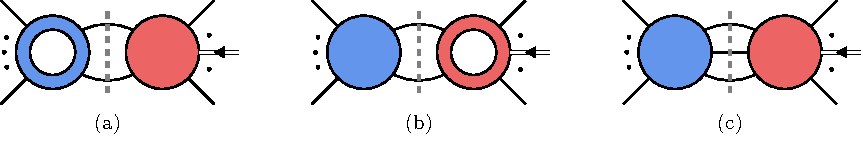
\includegraphics[page=1]{images/cuts.pdf}
    \caption{Unitarity cuts relevant for the extraction of anomalous dimensions from two-loop form factors. Higher-dimensional operator insertions are indicated by red blobs. The blobs with a hole denote one-loop form factors or amplitudes.}
    \label{fig:cuts}
\end{figure}
%%%%%%%%%%%%%%%%%%%%%%%%%%%%%%%%%%

The one-loop logic survives or fails cut by cut.
The genuinely new feature at two loops is that cuts (a) and (b) contain one-loop objects --- the renormalized amplitude $\mathcal M^{(1)}$ and the renormalized form factor $F^{(1)}_j$ --- whose finite rational parts are not determined by four-dimensional unitarity cuts.
It is precisely through such rational terms that one-loop amplitudes evade the tree-level helicity selection rules: for instance, the all-plus vector amplitude is non-zero, is UV and IR finite, and carries the minimal weight $w=0$.
Sewing it into cut (a) through \Eq{eq:sewing} gives $w_i \ge 0 + w_j - 4 = w_j - 4$,
so the one-loop bound can relax by as much as four units.
Whether the two-loop selection rule survives therefore depends entirely on controlling the rational parts of these one-loop objects.
Accordingly, we separate the two-loop zeros into those requiring no rational-part information, which are scheme independent, and those sensitive to it, which are scheme dependent.

\section{Scheme-Independent Zeros\label{sec:2loopSI}}

We first establish the selection rule at two loops, where the relevant mixing is fixed by tree-level
data alone and is therefore scheme independent.
Its extension to arbitrary loop order then follows from the same length and helicity counting, as we
discuss below.

At two loops, the length selection rule of Ref.~\cite{Bern:2019wie} already forbids a large class of entries: the form-factor side of any cut of $\mathcal O_j$ appearing in Eq.~\eqref{eq:master} needs at least $\ell_j$ legs, so an operator $\mathcal O_j$ cannot renormalize a shorter operator $\mathcal O_i$ at two loops when $\ell_j - \ell_i \ge 2$, since no such diagram can avoid a scaleless integral. Thus,
\begin{equation}
    \gamma^{(2)}_{ij} = 0 \ \ \ \text{if} \ \ \ \ell_i < \ell_j - 1\,.
\end{equation}

At the boundary $\ell_i = \ell_j - 1$, since $\gamma_{ij}^{(1)} = 0$, the operator mixing first occurs at two loops, and leg counting collapses the master formula in \Eq{eq:master} onto the single cut (c).
Indeed, the $\beta$-function term $\delta_{kj}\sum_g\beta^{(1)}_g\,\partial/\partial g\,\Re F^{(1)}_k$ is proportional to a form factor of $\Op_j$ itself, which is non-zero only on an external state with at least $\ell_j$ legs (configurations with fewer legs are forbidden by the particle content at tree level and force scaleless integrals at one loop \cite{Bern:2019wie}), whereas $X_i$ carries only $\ell_i=\ell_j-1$.
The IR term vanishes because it dresses $F^{(0)}_j(X_i)$ and $F^{(1)}_j(X_i)$, which are zero for $\ell_i < \ell_j$.
The iteration term $\Delta\gamma^{(1)}_{kj}\Re F^{(1)}_k(X_i)$ vanishes by the same counting applied twice: $\Delta\gamma^{(1)}_{kj}\neq0$ requires $\ell_k\ge\ell_j$, while $F^{(1)}_k(X_i)\neq0$ requires $\ell_i\ge\ell_k$, so together $\ell_i\ge\ell_j$.
Cuts (a) and (b) are likewise absent: a non-vanishing two-particle cut requires at least four legs on
the amplitude side, while tree and one-loop form factors of $\mathcal O_j$ require at least $\ell_j$
legs, since lower-multiplicity one-loop diagrams contain scaleless tadpoles or bubbles
\cite{Bern:2019wie,Bern:2020ikv,EliasMiro:2020tdv,Caron-Huot:2016cwu,EliasMiro:2021jgu}. Thus, they
yield at least $4+\ell_j-4=\ell_j>\ell_i$ external legs and Eq.~\eqref{eq:master} reduces to
\begin{equation}
    \gamma_{ij}^{(2)}\, F_{i}^{(0)}(X_i) = -\frac{1}{\pi} \left(\M^{(0)} \otimes_3  F^{(0)}_j\right)\left(X_i\right)\,,
\end{equation}
where $\M^{(0)}$ is necessarily a five-point amplitude.
Therefore, the tree-level helicity selection rule promotes to two loops exactly as at one loop. With three sewn legs, \Eq{eq:sewing} gives $w_i \ge 4 + w_j - 6$, so that
\begin{equation}
\label{eq:dl1}
    \gamma^{(2)}_{ij} = 0 \ \ \ \text{if} \ \ \ \ell_i = \ell_j - 1 \ \land \  \big(w_i < w_j - 2  \ \lor  \ \wb_i < \wb_j - 2\big) \,,
\end{equation}
absent non-holomorphic Yukawa couplings, which relax the weight conditions by two units.
%
The length selection rule implies that this mixing first arises at two loops, where its only
surviving contribution is built from four-dimensional tree amplitudes and tree form factors
integrated over four-dimensional phase space.
Finite renormalizations that preserve the length selection rule cannot feed this entry through
lower-order counterterms, so the zeros in \Eq{eq:dl1} remain unchanged under such changes of scheme.

The same logic extends to arbitrary loop order. At $L+1\ge 2$ loops with $\ell_i=\ell_j-L$, all
contributions to $\gamma^{(L+1)}_{ij}$ proportional to an IR anomalous dimension, a $\beta$-function,
or a lower-loop anomalous dimension, as well as every cut with a loop-level amplitude or form factor,
are excluded by the leg counting used above, each requiring $\ell_i\ge\ell_j-L+1$
\cite{Bern:2019wie}. As a consequence, only the maximal $(L+2)$-particle cut of tree amplitudes and
tree form factors survives, so that from Eq.~\eqref{eq:sewing} we obtain
\begin{equation}
\label{eq:gen}
    \gamma^{(L+1)}_{ij} = 0  \ \ \ \text{if} \ \  \ \ell_i = \ell_j-L \ \land \  \big(w_i < w_j - 2L  \ \lor  \ \wb_i < \wb_j - 2L\big) \,,
\end{equation}
with the last two conditions becoming $w_i < w_j - 2(L+1)$ and $\wb_i < \wb_j - 2(L+1)$ in the
presence of non-holomorphic Yukawa couplings.
For $\ell_i<\ell_j-L$ even the maximal cut is unavailable, so
\begin{equation}
    \gamma^{(L+1)}_{ij} = 0  \ \ \ \text{if} \ \  \ \ell_i < \ell_j-L\,.
\end{equation}

\section{Scheme-Dependent Two-Loop Zeros\label{sec:2loopSD}}

Subject to the complex-collinear factorization assumption discussed below, we find the following
extension to $\ell_i \ge \ell_j$:
\begin{equation}
\label{eq:dl2}
 \widehat\gamma^{(2)}_{ij} = 0 \  \ \ \text{if} \  \ \ \ell_i \ge \ell_j \ \land \  \big(w_i < w_j - 4 \  \lor  \ \wb_i < \wb_j - 4 \big) \,.
\end{equation}
Here the hat denotes the \textit{holomorphic scheme}, in which these zeros hold even in the presence
of non-holomorphic Yukawa couplings.
The key ingredient is the decomposition of the finite rational one-loop form factor, valid for
$w(X)<w_j-2$ or $\wb(X)<\wb_j-2$,
\begin{equation}
\label{eq:contact}
F^{(1)}_j(X) = \sum_i \kappa^{(1)}_{ij}\, F^{(0)}_i(X) \,,
\end{equation}
where $\kappa^{(1)}_{ij}$ are coefficients that depend only on the marginal couplings and the
renormalization prescription, and the sum runs over dimension-$d$ operators with $\ell_j\le\ell_i\le
d$ whose tree form factors are non-zero on $X$.
Removing these terms by the one-loop finite operator redefinition
$\widehat{\mathcal O}_j=\sum_i(\delta_{ij}-\kappa^{(1)}_{ij})\mathcal O_i$ defines the holomorphic
scheme.

In a generic scheme, such as $\MSbar$, the entries in the region of \Eq{eq:dl2} are generally
non-zero but satisfy
\begin{equation}
\label{eq:onedet}
    \gamma^{(2)}_{ij} = -[\kappa^{(1)},\gamma^{(1)}]_{ij} - \sum_g\beta_g^{(1)}\frac{\partial}{\partial g} \kappa^{(1)}_{ij} \,,
\end{equation}
with $[\kappa^{(1)},\gamma^{(1)}]_{ij}=\sum_k(\kappa^{(1)}_{ik}\gamma^{(1)}_{kj}-\gamma^{(1)}_{ik}\kappa^{(1)}_{kj})$.
Thus, this block carries no independent two-loop information: it is fixed entirely by the one-loop
anomalous dimensions, $\beta$-functions, and coefficients $\kappa^{(1)}_{ij}$.
The latter are read off from \Eq{eq:contact} on the minimal target configurations $X_i$, so no
two-loop integral is required.

The derivation of the existence of the holomorphic scheme is given in
Appendix~\ref{app:holomorphicscheme}. It assumes that the singularities of one-loop rational form
factors in complex-collinear limits retain a factorized form compatible with the helicity-weight
counting.
No general theorem establishes this factorization for complex momenta, where double and unreal poles
can occur \cite{Bern:2005hs,Bern:2005ji,Bern:2005cq}, and Eqs.~\eqref{eq:dl2}--\eqref{eq:onedet} are
therefore conditional on this assumption.
The scheme-independent two-loop zeros of \Eq{eq:dl1} and their higher-loop generalization in
\Eq{eq:gen} rely only on tree-level data and do not depend on this assumption.

\section{Applications\label{sec:2loopapplications}}

As a concrete application of these results, we summarize in Tables~\ref{tab:dim5}, \ref{tab:dim6},
\ref{tab:dim7}, and \ref{tab:dim8} the structure that the selection rules of
Eqs.~\eqref{eq:gen} and \eqref{eq:dl2} impose on the anomalous-dimension matrix at operator
dimensions five, six, seven, and eight, respectively.

\begin{table}[h!t!b!]
    \centering
    \renewcommand{\arraystretch}{1.3}
    \begin{NiceTabular}{cc|ccc|ccc|c}
         & & $\phi F^2$ & $\psi^2 F$ & $\psi^2\phi^2$ & $\phi \bar F^2$ & $\bar\psi^2 \bar F$ & $\bar \psi^2\phi^2$ & $\phi^5$ \\
         & $(w,\wb)$& $(1,5)$ & $(1,5)$ & $(3,5)$ & $(5,1)$ & $(5,1)$ & $(5,3)$ & $(5,5)$
         \\ \hline
         $\phi F^2$&$(1,5)$&&&\ccol&&&\ccol$\mathsf{H}$&$\mathsf{L}$\\
         $\psi^2 F$&$(1,5)$&&&\ccol&&&\ccol$\mathsf{H}$&$\mathsf{L}$\\
         $\psi^2 \phi^2$&$(3,5)$&&&&&&&\ccol\\ \hline
         $\phi \bar F^2$&$(5,1)$&&&\ccol$\mathsf{H}$&&&\ccol&$\mathsf{L}$\\
         $\bar \psi^2 \bar F$&$(5,1)$&&&\ccol$\mathsf{H}$&&&\ccol&$\mathsf{L}$\\
         $\bar \psi^2 \phi^2$&$(5,3)$&&&&&&&\ccol\\ \hline
         $\phi^5$&$(5,5)$&&&&&&&\\
    \end{NiceTabular}
    \caption{Structure of the two-loop anomalous-dimension matrix for dimension-five operators. The entry in row $\mathcal O_i$ and column $\mathcal O_j$ corresponds to $\gamma^{(2)}_{ij}$. Entries labeled $\mathsf{L}$ vanish by the length selection rule \cite{Bern:2019wie}. The shaded cells define the scheme-independent band $\ell_i=\ell_j-1$, which is completely determined by three-particle cuts of tree-level objects. Within this band, $\mathsf{H}$ denotes entries that vanish by the helicity selection rule of \Eq{eq:dl1}.}
    \label{tab:dim5}
\end{table}
\begin{table}[h!t!b!]
    \centering
    \renewcommand{\arraystretch}{1.3}
    \resizebox{\textwidth}{!}{%
    \begin{NiceTabular}{cc|ccccc|ccccc|cccc}
         & & $F^3$ & $\phi^2 F^2$ & $\psi^2\phi F$ & $\psi^4$ & $\psi^2\phi^3$ & $\bar F^3$ & $\phi^2\bar F^2$ & $\bar\psi^2\phi\bar F$ & $\bar\psi^4$ & $\bar\psi^2\phi^3$ & $\bar\psi^2\psi^2$ & $D\bar\psi\psi\phi^2$ & $D^2\phi^4$ & $\phi^6$ \\
         & $(w,\wb)$ & $(0,6)$ & $(2,6)$ & $(2,6)$ & $(2,6)$ & $(4,6)$ & $(6,0)$ & $(6,2)$ & $(6,2)$ & $(6,2)$ & $(6,4)$ & $(4,4)$ & $(4,4)$ & $(4,4)$ & $(6,6)$ \\ \hline
%        $F^3$ & $(0,6)$ & & & & & $\mathsf{L}$ & $\mathsf{H}^\star$ & \ccol$\mathsf{H}$ & \ccol$\mathsf{H}$ & \ccol$\mathsf{H}$ & $\mathsf{L}$ & \ccol$y^2$ & \ccol$y^2$ & \ccol$y^2$ & $\mathsf{L}$ \\
        $F^3$ & $(0,6)$ & & \ccol & \ccol & \ccol$\times$ & $\mathsf{L}$ & $\mathsf{H}^\star$ & \ccol$\mathsf{H}$ & \ccol$\mathsf{H}$ & \ccol$\mathsf{H}$ & $\mathsf{L}$ & \ccol$\mathsf{H}$ & \ccol$\mathsf{H}$ & \ccol$\mathsf{H}$ & $\mathsf{L}$ \\
        $\phi^2 F^2$ & $(2,6)$ & & & & & \ccol & & & & & \ccol$\mathsf{H}$ & & & & $\mathsf{L}$ \\
        $\psi^2\phi F$ & $(2,6)$ & & & & & \ccol & & & & & \ccol$\mathsf{H}$ & & & & $\mathsf{L}$ \\
        $\psi^4$ & $(2,6)$ & & & & & \ccol & & & & & \ccol$\mathsf{H}$ & & & & $\mathsf{L}$ \\
        $\psi^2\phi^3$ & $(4,6)$ & & & & & & & & & & & & & & \ccol \\ \hline
%        $\bar F^3$ & $(6,0)$ & $\mathsf{H}^\star$ & \ccol$\mathsf{H}$ & \ccol$\mathsf{H}$ & \ccol$\mathsf{H}$ & $\mathsf{L}$ & & & & & $\mathsf{L}$ & \ccol$\bar y^2$ & \ccol$\bar y^2$ & \ccol$\bar y^2$ & $\mathsf{L}$ \\
        $\bar F^3$ & $(6,0)$ & $\mathsf{H}^\star$ & \ccol$\mathsf{H}$ & \ccol$\mathsf{H}$ & \ccol$\mathsf{H}$ & $\mathsf{L}$ & & \ccol & \ccol & \ccol$\times$ & $\mathsf{L}$ & \ccol$\mathsf{H}$ & \ccol$\mathsf{H}$ & \ccol$\mathsf{H}$ & $\mathsf{L}$ \\
        $\phi^2\bar F^2$ & $(6,2)$ & & & & & \ccol$\mathsf{H}$ & & & & & \ccol & & & & $\mathsf{L}$ \\
        $\bar\psi^2\phi\bar F$ & $(6,2)$ & & & & & \ccol$\mathsf{H}$ & & & & & \ccol & & & & $\mathsf{L}$ \\
        $\bar\psi^4$ & $(6,2)$ & & & & & \ccol$\mathsf{H}$ & & & & & \ccol & & & & $\mathsf{L}$ \\
        $\bar\psi^2\phi^3$ & $(6,4)$ & & & & & & & & & & & & & & \ccol \\ \hline
        $\bar\psi^2\psi^2$ & $(4,4)$ & & & & & \ccol & & & & & \ccol & & & & $\mathsf{L}$ \\
        $D\bar\psi\psi\phi^2$ & $(4,4)$ & & & & & \ccol & & & & & \ccol & & & & $\mathsf{L}$ \\
        $D^2\phi^4$ & $(4,4)$ & & & & & \ccol & & & & & \ccol & & & & $\mathsf{L}$ \\
        $\phi^6$ & $(6,6)$ & & & & & & & & & & & & & & \\
    \end{NiceTabular}
    }
    \caption{Structure of the two-loop anomalous-dimension matrix for dimension-six operators. The entry in row $\mathcal O_i$ and column $\mathcal O_j$ corresponds to $\gamma^{(2)}_{ij}$. Entries labeled $\mathsf{L}$ vanish by the length selection rule \cite{Bern:2019wie}. The shaded cells define the scheme-independent band $\ell_i=\ell_j-1$, which is completely determined by three-particle cuts of tree-level objects. Within this band, $\mathsf{H}$ denotes entries that vanish by the helicity selection rule of \Eq{eq:dl1}. When the conditions of \Eq{eq:dl1} are not satisfied, $\times$ indicates entries for which no three-particle cuts exist. Finally, entries labeled $\mathsf{H}^\star$ vanish in the holomorphic scheme, as dictated by \Eq{eq:dl2}.}
    \label{tab:dim6}
\end{table}
\begin{sidewaystable}[p]
    \centering
    \renewcommand{\arraystretch}{1.3}
    \resizebox{\textheight}{!}{
    \begin{NiceTabular}[colortbl-like]{cc|ccccccccccc|ccccccccccc|cccc}
         & & $\phi F^3$ & $\psi^2 F^2$ & $D^2 \phi^3 F$ & $D \overline\psi \psi \phi F$ & $\overline\psi^2 F^2$ & $D^2 \psi^2 \phi^2$ & $D \overline\psi \psi^3$ & $\phi^3 F^2$ & $\psi^4 \phi$ & $\psi^2 \phi^2 F$ & $\psi^2 \phi^4$ & $\phi \overline F^3$ & $\overline\psi^2 \overline F^2$ & $D^2 \phi^3 \overline F$ & $D \overline\psi \psi \phi \overline F$ & $\psi^2 \overline F^2$ & $D^2 \overline\psi^2 \phi^2$ & $D \overline\psi^3 \psi$ & $\phi^3 \overline F^2$ & $\overline\psi^4 \phi$ & $\overline\psi^2 \phi^2 \overline F$ & $\overline\psi^2 \phi^4$ & $D^2 \phi^5$ & $D \overline\psi \psi \phi^3$ & $\overline\psi^2 \psi^2 \phi$ & $\phi^7$ \\
         & $(w,\wb)$ & $(1,7)$ & $(1,7)$ & $(3,5)$ & $(3,5)$ & $(3,5)$ & $(3,5)$ & $(3,5)$ & $(3,7)$ & $(3,7)$ & $(3,7)$ & $(5,7)$ & $(7,1)$ & $(7,1)$ & $(5,3)$ & $(5,3)$ & $(5,3)$ & $(5,3)$ & $(5,3)$ & $(7,3)$ & $(7,3)$ & $(7,3)$ & $(7,5)$ & $(5,5)$ & $(5,5)$ & $(5,5)$ & $(7,7)$ \\ \hline
        $\phi F^3$ & $(1,7)$ & $(1)$ & $(1)$ & $0_{(1)}$ & $0_{(1)}$ & $0_{(1)}$ & $0_{(1)}$ & $0_{(1)}$ & $(2)$ & \new $\times_{(2)}$ & $(2)$ & \new $\times_{(3)}$ & \ccol$0_{(1)}$ & \ccol$0_{(1)}$ & $0_{(1)}$ & $0_{(1)}$ & $0_{(1)}$ & $0_{(1)}$ & $0_{(1)}$ & \new $0_{(2)}$ & \new $0_{(2)}$ & \new $0_{(2)}$ & \new $0_{(3)}$ & \new $0_{(2)}$ & \new $0_{(2)}$ & \new $0_{(2)}$ & \new $\times_{(4)}$ \\
        $\psi^2 F^2$ & $(1,7)$ & $(1)$ & $(1)$ & $0_{(1)}$ & $0_{(1)}$ & $y^2_{(1)}$ & $0_{(1)}$ & $0_{(1)}$ & $(2)$ & $(2)$ & $(2)$ & $(3)$ & \ccol$0_{(1)}$ & \ccol$0_{(1)}$ & $0_{(1)}$ & $0_{(1)}$ & $0_{(1)}$ & $0_{(1)}$ & $0_{(1)}$ & \new $0_{(2)}$ & \new $0_{(2)}$ & \new $0_{(2)}$ & \new $0_{(3)}$ & \new $0_{(2)}$ & \new $0_{(2)}$ & \new $0_{(2)}$ & \new $\times_{(4)}$ \\
        $D^2 \phi^3 F$ & $(3,5)$ & $0_{(1)}$ & $0_{(1)}$ & $(1)$ & $(1)$ & $\times_{(1)}$ & $(1)$ & $\times_{(1)}$ & $(2)$ & \new $\times_{(2)}$ & $(2)$ & $(3)$ & $0_{(1)}$ & $0_{(1)}$ & $0_{(1)}$ & $0_{(1)}$ & $0_{(1)}$ & $0_{(1)}$ & $0_{(1)}$ & \new $0_{(2)}$ & \new $0_{(2)}$ & \new $0_{(2)}$ & $(3)$ & $(2)$ & $(2)$ & \new $\times_{(2)}$ & $(4)$ \\
        $D \overline\psi \psi \phi F$ & $(3,5)$ & $0_{(1)}$ & $0_{(1)}$ & $(1)$ & $(1)$ & $(1)$ & $(1)$ & $(1)$ & $(2)$ & $(2)$ & $(2)$ & $(3)$ & $0_{(1)}$ & $0_{(1)}$ & $0_{(1)}$ & $0_{(1)}$ & $0_{(1)}$ & $0_{(1)}$ & $0_{(1)}$ & \new $0_{(2)}$ & \new $y^2_{(2)}$ & \new $0_{(2)}$ & $(3)$ & \new $\times_{(2)}$ & $(2)$ & $(2)$ & \new $\times_{(4)}$ \\
        $\overline\psi^2 F^2$ & $(3,5)$ & $0_{(1)}$ & $\overline y^2_{(1)}$ & $\times_{(1)}$ & $(1)$ & $(1)$ & $\times_{(1)}$ & $\times_{(1)}$ & $(2)$ & \new $\times_{(2)}$ & \new $\times_{(2)}$ & \new $\times_{(3)}$ & $0_{(1)}$ & $0_{(1)}$ & $0_{(1)}$ & $0_{(1)}$ & $0_{(1)}$ & $0_{(1)}$ & $0_{(1)}$ & \new $0_{(2)}$ & \new $0_{(2)}$ & \new $0_{(2)}$ & $(3)$ & \new $\times_{(2)}$ & \new $\times_{(2)}$ & $(2)$ & \new $\times_{(4)}$ \\
        $D^2 \psi^2 \phi^2$ & $(3,5)$ & $0_{(1)}$ & $0_{(1)}$ & $(1)$ & $(1)$ & $\times_{(1)}$ & $(1)$ & $(1)$ & $(2)$ & $(2)$ & $(2)$ & $(3)$ & $0_{(1)}$ & $0_{(1)}$ & $0_{(1)}$ & $0_{(1)}$ & $0_{(1)}$ & $y^2_{(1)}$ & $0_{(1)}$ & \new $0_{(2)}$ & \new $0_{(2)}$ & \new $y^2_{(2)}$ & $(3)$ & $(2)$ & $(2)$ & $(2)$ & $(4)$ \\
        $D \overline\psi \psi^3$ & $(3,5)$ & $0_{(1)}$ & $0_{(1)}$ & $\times_{(1)}$ & $(1)$ & $\times_{(1)}$ & $(1)$ & $(1)$ & \new $\times_{(2)}$ & $(2)$ & $(2)$ & $(3)$ & $0_{(1)}$ & $0_{(1)}$ & $0_{(1)}$ & $0_{(1)}$ & $0_{(1)}$ & $0_{(1)}$ & $y^2_{(1)}$ & \new $0_{(2)}$ & \new $0_{(2)}$ & \new $0_{(2)}$ & \new $\times_{(3)}$ & \new $\times_{(2)}$ & $(2)$ & $(2)$ & \new $\times_{(4)}$ \\
        $\phi^3 F^2$ & $(3,7)$ & $(1)$ & $(1)$ & $(1)$ & $(1)$ & $(1)$ & $(1)$ & $\times_{(1)}$ & $(1)$ & $\times_{(1)}$ & $(1)$ & $(2)$ & $0_{(1)}$ & $0_{(1)}$ & $0_{(1)}$ & $0_{(1)}$ & $0_{(1)}$ & $0_{(1)}$ & $0_{(1)}$ & $0_{(1)}$ & $0_{(1)}$ & $0_{(1)}$ & \new $0_{(2)}$ & $0_{(1)}$ & $0_{(1)}$ & $0_{(1)}$ & $(3)$ \\
        $\psi^4 \phi$ & $(3,7)$ & $\times_{(1)}$ & $(1)$ & $\times_{(1)}$ & $(1)$ & $\times_{(1)}$ & $(1)$ & $(1)$ & $\times_{(1)}$ & $(1)$ & $(1)$ & $(2)$ & $0_{(1)}$ & $0_{(1)}$ & $0_{(1)}$ & $y^2_{(1)}$ & $0_{(1)}$ & $0_{(1)}$ & $0_{(1)}$ & $0_{(1)}$ & $0_{(1)}$ & $0_{(1)}$ & \new $0_{(2)}$ & $0_{(1)}$ & $0_{(1)}$ & $y^2_{(1)}$ & \new $\times_{(3)}$ \\
        $\psi^2 \phi^2 F$ & $(3,7)$ & $(1)$ & $(1)$ & $(1)$ & $(1)$ & $\times_{(1)}$ & $(1)$ & $(1)$ & $(1)$ & $(1)$ & $(1)$ & $(2)$ & $0_{(1)}$ & $0_{(1)}$ & $0_{(1)}$ & $0_{(1)}$ & $0_{(1)}$ & $y^2_{(1)}$ & $0_{(1)}$ & $0_{(1)}$ & $0_{(1)}$ & $0_{(1)}$ & \new $0_{(2)}$ & $0_{(1)}$ & $0_{(1)}$ & $0_{(1)}$ & \new $\times_{(3)}$ \\
        $\psi^2 \phi^4$ & $(5,7)$ & $\times_{(1)}$ & $(1)$ & $(1)$ & $(1)$ & $\times_{(1)}$ & $(1)$ & $(1)$ & $(1)$ & $(1)$ & $(1)$ & $(1)$ & $0_{(1)}$ & $0_{(1)}$ & $(1)$ & $(1)$ & $(1)$ & $(1)$ & $\times_{(1)}$ & $0_{(1)}$ & $0_{(1)}$ & $0_{(1)}$ & $y^2_{(1)}$ & $(1)$ & $(1)$ & $(1)$ & $(2)$ \\ \hline
        $\phi \overline F^3$ & $(7,1)$ & \ccol$0_{(1)}$ & \ccol$0_{(1)}$ & $0_{(1)}$ & $0_{(1)}$ & $0_{(1)}$ & $0_{(1)}$ & $0_{(1)}$ & \new $0_{(2)}$ & \new $0_{(2)}$ & \new $0_{(2)}$ & \new $0_{(3)}$ & $(1)$ & $(1)$ & $0_{(1)}$ & $0_{(1)}$ & $0_{(1)}$ & $0_{(1)}$ & $0_{(1)}$ & $(2)$ & \new $\times_{(2)}$ & $(2)$ & \new $\times_{(3)}$ & \new $0_{(2)}$ & \new $0_{(2)}$ & \new $0_{(2)}$ & \new $\times_{(4)}$ \\
        $\overline\psi^2 \overline F^2$ & $(7,1)$ & \ccol$0_{(1)}$ & \ccol$0_{(1)}$ & $0_{(1)}$ & $0_{(1)}$ & $0_{(1)}$ & $0_{(1)}$ & $0_{(1)}$ & \new $0_{(2)}$ & \new $0_{(2)}$ & \new $0_{(2)}$ & \new $0_{(3)}$ & $(1)$ & $(1)$ & $0_{(1)}$ & $0_{(1)}$ & $\overline y^2_{(1)}$ & $0_{(1)}$ & $0_{(1)}$ & $(2)$ & $(2)$ & $(2)$ & $(3)$ & \new $0_{(2)}$ & \new $0_{(2)}$ & \new $0_{(2)}$ & \new $\times_{(4)}$ \\
        $D^2 \phi^3 \overline F$ & $(5,3)$ & $0_{(1)}$ & $0_{(1)}$ & $0_{(1)}$ & $0_{(1)}$ & $0_{(1)}$ & $0_{(1)}$ & $0_{(1)}$ & \new $0_{(2)}$ & \new $0_{(2)}$ & \new $0_{(2)}$ & $(3)$ & $0_{(1)}$ & $0_{(1)}$ & $(1)$ & $(1)$ & $\times_{(1)}$ & $(1)$ & $\times_{(1)}$ & $(2)$ & \new $\times_{(2)}$ & $(2)$ & $(3)$ & $(2)$ & $(2)$ & \new $\times_{(2)}$ & $(4)$ \\
        $D \overline\psi \psi \phi \overline F$ & $(5,3)$ & $0_{(1)}$ & $0_{(1)}$ & $0_{(1)}$ & $0_{(1)}$ & $0_{(1)}$ & $0_{(1)}$ & $0_{(1)}$ & \new $0_{(2)}$ & \new $\overline y^2_{(2)}$ & \new $0_{(2)}$ & $(3)$ & $0_{(1)}$ & $0_{(1)}$ & $(1)$ & $(1)$ & $(1)$ & $(1)$ & $(1)$ & $(2)$ & $(2)$ & $(2)$ & $(3)$ & \new $\times_{(2)}$ & $(2)$ & $(2)$ & \new $\times_{(4)}$ \\
        $\psi^2 \overline F^2$ & $(5,3)$ & $0_{(1)}$ & $0_{(1)}$ & $0_{(1)}$ & $0_{(1)}$ & $0_{(1)}$ & $0_{(1)}$ & $0_{(1)}$ & \new $0_{(2)}$ & \new $0_{(2)}$ & \new $0_{(2)}$ & $(3)$ & $0_{(1)}$ & $y^2_{(1)}$ & $\times_{(1)}$ & $(1)$ & $(1)$ & $\times_{(1)}$ & $\times_{(1)}$ & $(2)$ & \new $\times_{(2)}$ & \new $\times_{(2)}$ & \new $\times_{(3)}$ & \new $\times_{(2)}$ & \new $\times_{(2)}$ & $(2)$ & \new $\times_{(4)}$ \\
        $D^2 \overline\psi^2 \phi^2$ & $(5,3)$ & $0_{(1)}$ & $0_{(1)}$ & $0_{(1)}$ & $0_{(1)}$ & $0_{(1)}$ & $\overline y^2_{(1)}$ & $0_{(1)}$ & \new $0_{(2)}$ & \new $0_{(2)}$ & \new $\overline y^2_{(2)}$ & $(3)$ & $0_{(1)}$ & $0_{(1)}$ & $(1)$ & $(1)$ & $\times_{(1)}$ & $(1)$ & $(1)$ & $(2)$ & $(2)$ & $(2)$ & $(3)$ & $(2)$ & $(2)$ & $(2)$ & $(4)$ \\
        $D \overline\psi^3 \psi$ & $(5,3)$ & $0_{(1)}$ & $0_{(1)}$ & $0_{(1)}$ & $0_{(1)}$ & $0_{(1)}$ & $0_{(1)}$ & $\overline y^2_{(1)}$ & \new $0_{(2)}$ & \new $0_{(2)}$ & \new $0_{(2)}$ & \new $\times_{(3)}$ & $0_{(1)}$ & $0_{(1)}$ & $\times_{(1)}$ & $(1)$ & $\times_{(1)}$ & $(1)$ & $(1)$ & \new $\times_{(2)}$ & $(2)$ & $(2)$ & $(3)$ & \new $\times_{(2)}$ & $(2)$ & $(2)$ & \new $\times_{(4)}$ \\
        $\phi^3 \overline F^2$ & $(7,3)$ & $0_{(1)}$ & $0_{(1)}$ & $0_{(1)}$ & $0_{(1)}$ & $0_{(1)}$ & $0_{(1)}$ & $0_{(1)}$ & $0_{(1)}$ & $0_{(1)}$ & $0_{(1)}$ & \new $0_{(2)}$ & $(1)$ & $(1)$ & $(1)$ & $(1)$ & $(1)$ & $(1)$ & $\times_{(1)}$ & $(1)$ & $\times_{(1)}$ & $(1)$ & $(2)$ & $0_{(1)}$ & $0_{(1)}$ & $0_{(1)}$ & $(3)$ \\
        $\overline\psi^4 \phi$ & $(7,3)$ & $0_{(1)}$ & $0_{(1)}$ & $0_{(1)}$ & $\overline y^2_{(1)}$ & $0_{(1)}$ & $0_{(1)}$ & $0_{(1)}$ & $0_{(1)}$ & $0_{(1)}$ & $0_{(1)}$ & \new $0_{(2)}$ & $\times_{(1)}$ & $(1)$ & $\times_{(1)}$ & $(1)$ & $\times_{(1)}$ & $(1)$ & $(1)$ & $\times_{(1)}$ & $(1)$ & $(1)$ & $(2)$ & $0_{(1)}$ & $0_{(1)}$ & $\overline y^2_{(1)}$ & \new $\times_{(3)}$ \\
        $\overline\psi^2 \phi^2 \overline F$ & $(7,3)$ & $0_{(1)}$ & $0_{(1)}$ & $0_{(1)}$ & $0_{(1)}$ & $0_{(1)}$ & $\overline y^2_{(1)}$ & $0_{(1)}$ & $0_{(1)}$ & $0_{(1)}$ & $0_{(1)}$ & \new $0_{(2)}$ & $(1)$ & $(1)$ & $(1)$ & $(1)$ & $\times_{(1)}$ & $(1)$ & $(1)$ & $(1)$ & $(1)$ & $(1)$ & $(2)$ & $0_{(1)}$ & $0_{(1)}$ & $0_{(1)}$ & \new $\times_{(3)}$ \\
        $\overline\psi^2 \phi^4$ & $(7,5)$ & $0_{(1)}$ & $0_{(1)}$ & $(1)$ & $(1)$ & $(1)$ & $(1)$ & $\times_{(1)}$ & $0_{(1)}$ & $0_{(1)}$ & $0_{(1)}$ & $\overline y^2_{(1)}$ & $\times_{(1)}$ & $(1)$ & $(1)$ & $(1)$ & $\times_{(1)}$ & $(1)$ & $(1)$ & $(1)$ & $(1)$ & $(1)$ & $(1)$ & $(1)$ & $(1)$ & $(1)$ & $(2)$ \\ \hline
        $D^2 \phi^5$ & $(5,5)$ & $0_{(1)}$ & $0_{(1)}$ & $(1)$ & $\times_{(1)}$ & $\times_{(1)}$ & $(1)$ & $\times_{(1)}$ & $0_{(1)}$ & $0_{(1)}$ & $0_{(1)}$ & $(2)$ & $0_{(1)}$ & $0_{(1)}$ & $(1)$ & $\times_{(1)}$ & $\times_{(1)}$ & $(1)$ & $\times_{(1)}$ & $0_{(1)}$ & $0_{(1)}$ & $0_{(1)}$ & $(2)$ & $(1)$ & $(1)$ & $\times_{(1)}$ & $(3)$ \\
        $D \overline\psi \psi \phi^3$ & $(5,5)$ & $0_{(1)}$ & $0_{(1)}$ & $(1)$ & $(1)$ & $\times_{(1)}$ & $(1)$ & $(1)$ & $0_{(1)}$ & $0_{(1)}$ & $0_{(1)}$ & $(2)$ & $0_{(1)}$ & $0_{(1)}$ & $(1)$ & $(1)$ & $\times_{(1)}$ & $(1)$ & $(1)$ & $0_{(1)}$ & $0_{(1)}$ & $0_{(1)}$ & $(2)$ & $(1)$ & $(1)$ & $(1)$ & $(3)$ \\
        $\overline\psi^2 \psi^2 \phi$ & $(5,5)$ & $0_{(1)}$ & $0_{(1)}$ & $\times_{(1)}$ & $(1)$ & $(1)$ & $(1)$ & $(1)$ & $0_{(1)}$ & $\overline y^2_{(1)}$ & $0_{(1)}$ & $(2)$ & $0_{(1)}$ & $0_{(1)}$ & $\times_{(1)}$ & $(1)$ & $(1)$ & $(1)$ & $(1)$ & $0_{(1)}$ & $y^2_{(1)}$ & $0_{(1)}$ & $(2)$ & $\times_{(1)}$ & $(1)$ & $(1)$ & \new $\times_{(3)}$ \\
        $\phi^7$ & $(7,7)$ & $\times_{(1)}$ & $\times_{(1)}$ & $(1)$ & $\times_{(1)}$ & $\times_{(1)}$ & $(1)$ & $\times_{(1)}$ & $(1)$ & $\times_{(1)}$ & $\times_{(1)}$ & $(1)$ & $\times_{(1)}$ & $\times_{(1)}$ & $(1)$ & $\times_{(1)}$ & $\times_{(1)}$ & $(1)$ & $\times_{(1)}$ & $(1)$ & $\times_{(1)}$ & $\times_{(1)}$ & $(1)$ & $(1)$ & $(1)$ & $\times_{(1)}$ & $(1)$ \\
    \end{NiceTabular}
    }
    \caption{Structure of the anomalous-dimension matrix for general dimension-seven operators. The notation is described in Table \ref{tab:dim5}.}
    \label{tab:dim7}
\end{sidewaystable}
%\begin{landscape}
\begin{sidewaystable}[p]
    \centering
    \renewcommand{\arraystretch}{1.3}
    %\setlength{\tabcolsep}{2pt}
    \resizebox{\textheight}{!}{%
    \begin{NiceTabular}[colortbl-like]{cc|cccccccccccccccccc|cccccccccccccccccc|cccc}
         & & $F^4$ & $D^2\phi^2F^2$ & $D^2\psi^2\phi F$ & $D^2\psi^4$ & $D\bar\psi\psi F^2$ & $\phi^2 F^3$ & $\psi^2\phi F^2$ & $\psi^4 F$ & $D^2\phi^4 F$ & $D^2\psi^2\phi^3$ & $D\bar\psi\psi\phi^2 F$ & $D\bar\psi\psi^3\phi$ & $\bar\psi^2\phi F^2$ & $\bar\psi^2\psi^2 F$ & $\phi^4 F^2$ & $\psi^2\phi^3 F$ & $\psi^4\phi^2$ & $\psi^2\phi^5$ & $\bar F^4$ & $D^2\phi^2\bar F^2$ & $D^2\bar\psi^2\phi\bar F$ & $D^2\bar\psi^4$ & $D\bar\psi\psi\bar F^2$ & $\phi^2\bar F^3$ & $\bar\psi^2\phi\bar F^2$ & $\bar\psi^4\bar F$ & $D^2\phi^4\bar F$ & $D^2\bar\psi^2\phi^3$ & $D\bar\psi\psi\phi^2\bar F$ & $D\bar\psi^3\psi\phi$ & $\psi^2\phi\bar F^2$ & $\bar\psi^2\psi^2\bar F$ & $\phi^4\bar F^2$ & $\bar\psi^2\phi^3\bar F$ & $\bar\psi^4\phi^2$ & $\bar\psi^2\phi^5$ & $D^2\phi^6$ & $D\bar\psi\psi\phi^4$ & $\bar\psi^2\psi^2\phi^2$ & $\phi^8$ \\
         & $(w,\wb)$ & $(0,8)$ & $(2,6)$ & $(2,6)$ & $(2,6)$ & $(2,6)$ & $(2,8)$ & $(2,8)$ & $(2,8)$ & $(4,6)$ & $(4,6)$ & $(4,6)$ & $(4,6)$ & $(4,6)$ & $(4,6)$ & $(4,8)$ & $(4,8)$ & $(4,8)$ & $(6,8)$ & $(8,0)$ & $(6,2)$ & $(6,2)$ & $(6,2)$ & $(6,2)$ & $(8,2)$ & $(8,2)$ & $(8,2)$ & $(6,4)$ & $(6,4)$ & $(6,4)$ & $(6,4)$ & $(6,4)$ & $(6,4)$ & $(8,4)$ & $(8,4)$ & $(8,4)$ & $(8,6)$ & $(6,6)$ & $(6,6)$ & $(6,6)$ & $(8,8)$ \\ \hline
        $F^4$ & $(0,8)$ &  &  &  &  &  & \ccol & \ccol & \ccol$\times$ & \ccol$\mathsf{H}$ & \ccol$\mathsf{H}$ & \ccol$\mathsf{H}$ & \ccol$\mathsf{H}$ & \ccol$\mathsf{H}$ & \ccol$\mathsf{H}$ & $\mathsf{L}$ & $\mathsf{L}$ & $\mathsf{L}$ & $\mathsf{L}$ & $\mathsf{H}^\star$ & $\mathsf{H}^\star$ & $\mathsf{H}^\star$ & $\mathsf{H}^\star$ & $\mathsf{H}^\star$ & \ccol$\mathsf{H}$ & \ccol$\mathsf{H}$ & \ccol$\mathsf{H}$ & \ccol$\mathsf{H}$ & \ccol$\mathsf{H}$ & \ccol$\mathsf{H}$ & \ccol$\mathsf{H}$ & \ccol$\mathsf{H}$ & \ccol$\mathsf{H}$ & $\mathsf{L}$ & $\mathsf{L}$ & $\mathsf{L}$ & $\mathsf{L}$ & $\mathsf{L}$ & $\mathsf{L}$ & $\mathsf{L}$ & $\mathsf{L}$ \\
        $D^2\phi^2F^2$ & $(2,6)$ &  &  &  &  &  & \ccol & \ccol & \ccol$\times$ & \ccol & \ccol & \ccol & \ccol$\times$ & \ccol & \ccol$\times$ & $\mathsf{L}$ & $\mathsf{L}$ & $\mathsf{L}$ & $\mathsf{L}$ & $\mathsf{H}^\star$ &  &  &  &  & \ccol$\mathsf{H}$ & \ccol$\mathsf{H}$ & \ccol$\mathsf{H}$ & \ccol$\mathsf{H}$ & \ccol$\mathsf{H}$ & \ccol$\mathsf{H}$ & \ccol$\mathsf{H}$ & \ccol$\mathsf{H}$ & \ccol$\mathsf{H}$ & $\mathsf{L}$ & $\mathsf{L}$ & $\mathsf{L}$ & $\mathsf{L}$ & $\mathsf{L}$ & $\mathsf{L}$ & $\mathsf{L}$ & $\mathsf{L}$ \\
        $D^2\psi^2\phi F$ & $(2,6)$ &  &  &  &  &  & \ccol & \ccol & \ccol & \ccol & \ccol & \ccol & \ccol & \ccol & \ccol & $\mathsf{L}$ & $\mathsf{L}$ & $\mathsf{L}$ & $\mathsf{L}$ & $\mathsf{H}^\star$ &  &  &  &  & \ccol$\mathsf{H}$ & \ccol$\mathsf{H}$ & \ccol$\mathsf{H}$ & \ccol$\mathsf{H}$ & \ccol$\mathsf{H}$ & \ccol$\mathsf{H}$ & \ccol$y^2$ & \ccol$\mathsf{H}$ & \ccol$\mathsf{H}$ & $\mathsf{L}$ & $\mathsf{L}$ & $\mathsf{L}$ & $\mathsf{L}$ & $\mathsf{L}$ & $\mathsf{L}$ & $\mathsf{L}$ & $\mathsf{L}$ \\
        $D^2\psi^4$ & $(2,6)$ &  &  &  &  &  & \ccol$\times$ & \ccol & \ccol & \ccol$\times$ & \ccol & \ccol$\times$ & \ccol & \ccol$\times$ & \ccol & $\mathsf{L}$ & $\mathsf{L}$ & $\mathsf{L}$ & $\mathsf{L}$ & $\mathsf{H}^\star$ &  &  &  &  & \ccol$\mathsf{H}$ & \ccol$\mathsf{H}$ & \ccol$\mathsf{H}$ & \ccol$\mathsf{H}$ & \ccol$\mathsf{H}$ & \ccol$\mathsf{H}$ & \ccol$\mathsf{H}$ & \ccol$\mathsf{H}$ & \ccol$y^2$ & $\mathsf{L}$ & $\mathsf{L}$ & $\mathsf{L}$ & $\mathsf{L}$ & $\mathsf{L}$ & $\mathsf{L}$ & $\mathsf{L}$ & $\mathsf{L}$ \\
        $D\bar\psi\psi F^2$ & $(2,6)$ &  &  &  &  &  & \ccol & \ccol & \ccol & \ccol$\times$ & \ccol$\times$ & \ccol & \ccol & \ccol & \ccol & $\mathsf{L}$ & $\mathsf{L}$ & $\mathsf{L}$ & $\mathsf{L}$ & $\mathsf{H}^\star$ &  &  &  &  & \ccol$\mathsf{H}$ & \ccol$\mathsf{H}$ & \ccol$\mathsf{H}$ & \ccol$\mathsf{H}$ & \ccol$\mathsf{H}$ & \ccol$\mathsf{H}$ & \ccol$\mathsf{H}$ & \ccol$\mathsf{H}$ & \ccol$\mathsf{H}$ & $\mathsf{L}$ & $\mathsf{L}$ & $\mathsf{L}$ & $\mathsf{L}$ & $\mathsf{L}$ & $\mathsf{L}$ & $\mathsf{L}$ & $\mathsf{L}$ \\
        $\phi^2 F^3$ & $(2,8)$ &  &  &  &  &  &  &  &  &  &  &  &  &  &  & \ccol & \ccol & \ccol$\times$ & $\mathsf{L}$ & $\mathsf{H}^\star$ &  &  &  &  & $\mathsf{H}^\star$ & $\mathsf{H}^\star$ & $\mathsf{H}^\star$ &  &  &  &  &  &  & \ccol$\mathsf{H}$ & \ccol$\mathsf{H}$ & \ccol$\mathsf{H}$ & $\mathsf{L}$ & \ccol$\mathsf{H}$ & \ccol$\mathsf{H}$ & \ccol$\mathsf{H}$ & $\mathsf{L}$ \\
        $\psi^2\phi F^2$ & $(2,8)$ &  &  &  &  &  &  &  &  &  &  &  &  &  &  & \ccol & \ccol & \ccol & $\mathsf{L}$ & $\mathsf{H}^\star$ &  &  &  &  & $\mathsf{H}^\star$ & $\mathsf{H}^\star$ & $\mathsf{H}^\star$ &  &  &  &  &  &  & \ccol$\mathsf{H}$ & \ccol$\mathsf{H}$ & \ccol$\mathsf{H}$ & $\mathsf{L}$ & \ccol$\mathsf{H}$ & \ccol$\mathsf{H}$ & \ccol$\mathsf{H}$ & $\mathsf{L}$ \\
        $\psi^4 F$ & $(2,8)$ &  &  &  &  &  &  &  &  &  &  &  &  &  &  & \ccol$\times$ & \ccol & \ccol & $\mathsf{L}$ & $\mathsf{H}^\star$ &  &  &  &  & $\mathsf{H}^\star$ & $\mathsf{H}^\star$ & $\mathsf{H}^\star$ &  &  &  &  &  &  & \ccol$\mathsf{H}$ & \ccol$\mathsf{H}$ & \ccol$\mathsf{H}$ & $\mathsf{L}$ & \ccol$\mathsf{H}$ & \ccol$\mathsf{H}$ & \ccol$\mathsf{H}$ & $\mathsf{L}$ \\
        $D^2\phi^4 F$ & $(4,6)$ &  &  &  &  &  &  &  &  &  &  &  &  &  &  & \ccol & \ccol & \ccol$\times$ & $\mathsf{L}$ &  &  &  &  &  &  &  &  &  &  &  &  &  &  & \ccol$\mathsf{H}$ & \ccol$\mathsf{H}$ & \ccol$\mathsf{H}$ & $\mathsf{L}$ & \ccol & \ccol & \ccol$\times$ & $\mathsf{L}$ \\
        $D^2\psi^2\phi^3$ & $(4,6)$ &  &  &  &  &  &  &  &  &  &  &  &  &  &  & \ccol & \ccol & \ccol & $\mathsf{L}$ &  &  &  &  &  &  &  &  &  &  &  &  &  &  & \ccol$\mathsf{H}$ & \ccol$y^2$ & \ccol$\mathsf{H}$ & $\mathsf{L}$ & \ccol & \ccol & \ccol & $\mathsf{L}$ \\
        $D\bar\psi\psi\phi^2 F$ & $(4,6)$ &  &  &  &  &  &  &  &  &  &  &  &  &  &  & \ccol & \ccol & \ccol & $\mathsf{L}$ &  &  &  &  &  &  &  &  &  &  &  &  &  &  & \ccol$\mathsf{H}$ & \ccol$\mathsf{H}$ & \ccol$y^2$ & $\mathsf{L}$ & \ccol$\times$ & \ccol & \ccol & $\mathsf{L}$ \\
        $D\bar\psi\psi^3\phi$ & $(4,6)$ &  &  &  &  &  &  &  &  &  &  &  &  &  &  & \ccol$\times$ & \ccol & \ccol & $\mathsf{L}$ &  &  &  &  &  &  &  &  &  &  &  &  &  &  & \ccol$\mathsf{H}$ & \ccol$\mathsf{H}$ & \ccol$\mathsf{H}$ & $\mathsf{L}$ & \ccol$\times$ & \ccol & \ccol & $\mathsf{L}$ \\
        $\bar\psi^2\phi F^2$ & $(4,6)$ &  &  &  &  &  &  &  &  &  &  &  &  &  &  & \ccol & \ccol$\times$ & \ccol$\times$ & $\mathsf{L}$ &  &  &  &  &  &  &  &  &  &  &  &  &  &  & \ccol$\mathsf{H}$ & \ccol$\mathsf{H}$ & \ccol$\mathsf{H}$ & $\mathsf{L}$ & \ccol$\times$ & \ccol$\times$ & \ccol & $\mathsf{L}$ \\
        $\bar\psi^2\psi^2 F$ & $(4,6)$ &  &  &  &  &  &  &  &  &  &  &  &  &  &  & \ccol$\times$ & \ccol & \ccol$\times$ & $\mathsf{L}$ &  &  &  &  &  &  &  &  &  &  &  &  &  &  & \ccol$\mathsf{H}$ & \ccol$\mathsf{H}$ & \ccol$\mathsf{H}$ & $\mathsf{L}$ & \ccol$\times$ & \ccol$\times$ & \ccol & $\mathsf{L}$ \\
        $\phi^4 F^2$ & $(4,8)$ &  &  &  &  &  &  &  &  &  &  &  &  &  &  &  &  &  & \ccol &  &  &  &  &  &  &  &  &  &  &  &  &  &  &  &  &  & \ccol$\mathsf{H}$ &  &  &  & $\mathsf{L}$ \\
        $\psi^2\phi^3 F$ & $(4,8)$ &  &  &  &  &  &  &  &  &  &  &  &  &  &  &  &  &  & \ccol &  &  &  &  &  &  &  &  &  &  &  &  &  &  &  &  &  & \ccol$\mathsf{H}$ &  &  &  & $\mathsf{L}$ \\
        $\psi^4\phi^2$ & $(4,8)$ &  &  &  &  &  &  &  &  &  &  &  &  &  &  &  &  &  & \ccol &  &  &  &  &  &  &  &  &  &  &  &  &  &  &  &  &  & \ccol$\mathsf{H}$ &  &  &  & $\mathsf{L}$ \\
        $\psi^2\phi^5$ & $(6,8)$ &  &  &  &  &  &  &  &  &  &  &  &  &  &  &  &  &  &  &  &  &  &  &  &  &  &  &  &  &  &  &  &  &  &  &  &  &  &  &  & \ccol \\
        \hline
        $\bar F^4$ & $(8,0)$ & $\mathsf{H}^\star$ & $\mathsf{H}^\star$ & $\mathsf{H}^\star$ & $\mathsf{H}^\star$ & $\mathsf{H}^\star$ & \ccol$\mathsf{H}$ & \ccol$\mathsf{H}$ & \ccol$\mathsf{H}$ & \ccol$\mathsf{H}$ & \ccol$\mathsf{H}$ & \ccol$\mathsf{H}$ & \ccol$\mathsf{H}$ & \ccol$\mathsf{H}$ & \ccol$\mathsf{H}$ & $\mathsf{L}$ & $\mathsf{L}$ & $\mathsf{L}$ & $\mathsf{L}$ &  &  &  &  &  & \ccol & \ccol & \ccol$\times$ & \ccol$\mathsf{H}$ & \ccol$\mathsf{H}$ & \ccol$\mathsf{H}$ & \ccol$\mathsf{H}$ & \ccol$\mathsf{H}$ & \ccol$\mathsf{H}$ & $\mathsf{L}$ & $\mathsf{L}$ & $\mathsf{L}$ & $\mathsf{L}$ & $\mathsf{L}$ & $\mathsf{L}$ & $\mathsf{L}$ & $\mathsf{L}$ \\
        $D^2\phi^2\bar F^2$ & $(6,2)$ & $\mathsf{H}^\star$ &  &  &  &  & \ccol$\mathsf{H}$ & \ccol$\mathsf{H}$ & \ccol$\mathsf{H}$ & \ccol$\mathsf{H}$ & \ccol$\mathsf{H}$ & \ccol$\mathsf{H}$ & \ccol$\mathsf{H}$ & \ccol$\mathsf{H}$ & \ccol$\mathsf{H}$ & $\mathsf{L}$ & $\mathsf{L}$ & $\mathsf{L}$ & $\mathsf{L}$ &  &  &  &  &  & \ccol & \ccol & \ccol$\times$ & \ccol & \ccol & \ccol & \ccol$\times$ & \ccol & \ccol$\times$ & $\mathsf{L}$ & $\mathsf{L}$ & $\mathsf{L}$ & $\mathsf{L}$ & $\mathsf{L}$ & $\mathsf{L}$ & $\mathsf{L}$ & $\mathsf{L}$ \\
        $D^2\bar\psi^2\phi\bar F$ & $(6,2)$ & $\mathsf{H}^\star$ &  &  &  &  & \ccol$\mathsf{H}$ & \ccol$\mathsf{H}$ & \ccol$\mathsf{H}$ & \ccol$\mathsf{H}$ & \ccol$\mathsf{H}$ & \ccol$\mathsf{H}$ & \ccol$\bar y^2$ & \ccol$\mathsf{H}$ & \ccol$\mathsf{H}$ & $\mathsf{L}$ & $\mathsf{L}$ & $\mathsf{L}$ & $\mathsf{L}$ &  &  &  &  &  & \ccol & \ccol & \ccol & \ccol & \ccol & \ccol & \ccol & \ccol & \ccol & $\mathsf{L}$ & $\mathsf{L}$ & $\mathsf{L}$ & $\mathsf{L}$ & $\mathsf{L}$ & $\mathsf{L}$ & $\mathsf{L}$ & $\mathsf{L}$ \\
        $D^2\bar\psi^4$ & $(6,2)$ & $\mathsf{H}^\star$ &  &  &  &  & \ccol$\mathsf{H}$ & \ccol$\mathsf{H}$ & \ccol$\mathsf{H}$ & \ccol$\mathsf{H}$ & \ccol$\mathsf{H}$ & \ccol$\mathsf{H}$ & \ccol$\mathsf{H}$ & \ccol$\mathsf{H}$ & \ccol$\bar y^2$ & $\mathsf{L}$ & $\mathsf{L}$ & $\mathsf{L}$ & $\mathsf{L}$ &  &  &  &  &  & \ccol$\times$ & \ccol & \ccol & \ccol$\times$ & \ccol & \ccol$\times$ & \ccol & \ccol$\times$ & \ccol & $\mathsf{L}$ & $\mathsf{L}$ & $\mathsf{L}$ & $\mathsf{L}$ & $\mathsf{L}$ & $\mathsf{L}$ & $\mathsf{L}$ & $\mathsf{L}$ \\
        $D\bar\psi\psi\bar F^2$ & $(6,2)$ & $\mathsf{H}^\star$ &  &  &  &  & \ccol$\mathsf{H}$ & \ccol$\mathsf{H}$ & \ccol$\mathsf{H}$ & \ccol$\mathsf{H}$ & \ccol$\mathsf{H}$ & \ccol$\mathsf{H}$ & \ccol$\mathsf{H}$ & \ccol$\mathsf{H}$ & \ccol$\mathsf{H}$ & $\mathsf{L}$ & $\mathsf{L}$ & $\mathsf{L}$ & $\mathsf{L}$ &  &  &  &  &  & \ccol & \ccol & \ccol & \ccol$\times$ & \ccol$\times$ & \ccol & \ccol & \ccol & \ccol & $\mathsf{L}$ & $\mathsf{L}$ & $\mathsf{L}$ & $\mathsf{L}$ & $\mathsf{L}$ & $\mathsf{L}$ & $\mathsf{L}$ & $\mathsf{L}$ \\
        $\phi^2\bar F^3$ & $(8,2)$ & $\mathsf{H}^\star$ &  &  &  &  & $\mathsf{H}^\star$ & $\mathsf{H}^\star$ & $\mathsf{H}^\star$ &  &  &  &  &  &  & \ccol$\mathsf{H}$ & \ccol$\mathsf{H}$ & \ccol$\mathsf{H}$ & $\mathsf{L}$ &  &  &  &  &  &  &  &  &  &  &  &  &  &  & \ccol & \ccol & \ccol$\times$ & $\mathsf{L}$ & \ccol$\mathsf{H}$ & \ccol$\mathsf{H}$ & \ccol$\mathsf{H}$ & $\mathsf{L}$ \\
        $\bar\psi^2\phi\bar F^2$ & $(8,2)$ & $\mathsf{H}^\star$ &  &  &  &  & $\mathsf{H}^\star$ & $\mathsf{H}^\star$ & $\mathsf{H}^\star$ &  &  &  &  &  &  & \ccol$\mathsf{H}$ & \ccol$\mathsf{H}$ & \ccol$\mathsf{H}$ & $\mathsf{L}$ &  &  &  &  &  &  &  &  &  &  &  &  &  &  & \ccol & \ccol & \ccol & $\mathsf{L}$ & \ccol$\mathsf{H}$ & \ccol$\mathsf{H}$ & \ccol$\mathsf{H}$ & $\mathsf{L}$ \\
        $\bar\psi^4\bar F$ & $(8,2)$ & $\mathsf{H}^\star$ &  &  &  &  & $\mathsf{H}^\star$ & $\mathsf{H}^\star$ & $\mathsf{H}^\star$ &  &  &  &  &  &  & \ccol$\mathsf{H}$ & \ccol$\mathsf{H}$ & \ccol$\mathsf{H}$ & $\mathsf{L}$ &  &  &  &  &  &  &  &  &  &  &  &  &  &  & \ccol$\times$ & \ccol & \ccol & $\mathsf{L}$ & \ccol$\mathsf{H}$ & \ccol$\mathsf{H}$ & \ccol$\mathsf{H}$ & $\mathsf{L}$ \\
        $D^2\phi^4\bar F$ & $(6,4)$ &  &  &  &  &  &  &  &  &  &  &  &  &  &  & \ccol$\mathsf{H}$ & \ccol$\mathsf{H}$ & \ccol$\mathsf{H}$ & $\mathsf{L}$ &  &  &  &  &  &  &  &  &  &  &  &  &  &  & \ccol & \ccol & \ccol$\times$ & $\mathsf{L}$ & \ccol & \ccol & \ccol$\times$ & $\mathsf{L}$ \\
        $D^2\bar\psi^2\phi^3$ & $(6,4)$ &  &  &  &  &  &  &  &  &  &  &  &  &  &  & \ccol$\mathsf{H}$ & \ccol$\bar y^2$ & \ccol$\mathsf{H}$ & $\mathsf{L}$ &  &  &  &  &  &  &  &  &  &  &  &  &  &  & \ccol & \ccol & \ccol & $\mathsf{L}$ & \ccol & \ccol & \ccol & $\mathsf{L}$ \\
        $D\bar\psi\psi\phi^2\bar F$ & $(6,4)$ &  &  &  &  &  &  &  &  &  &  &  &  &  &  & \ccol$\mathsf{H}$ & \ccol$\mathsf{H}$ & \ccol$\bar y^2$ & $\mathsf{L}$ &  &  &  &  &  &  &  &  &  &  &  &  &  &  & \ccol & \ccol & \ccol & $\mathsf{L}$ & \ccol$\times$ & \ccol & \ccol & $\mathsf{L}$ \\
        $D\bar\psi^3\psi\phi$ & $(6,4)$ &  &  &  &  &  &  &  &  &  &  &  &  &  &  & \ccol$\mathsf{H}$ & \ccol$\mathsf{H}$ & \ccol$\mathsf{H}$ & $\mathsf{L}$ &  &  &  &  &  &  &  &  &  &  &  &  &  &  & \ccol$\times$ & \ccol & \ccol & $\mathsf{L}$ & \ccol$\times$ & \ccol & \ccol & $\mathsf{L}$ \\
        $\psi^2\phi\bar F^2$ & $(6,4)$ &  &  &  &  &  &  &  &  &  &  &  &  &  &  & \ccol$\mathsf{H}$ & \ccol$\mathsf{H}$ & \ccol$\mathsf{H}$ & $\mathsf{L}$ &  &  &  &  &  &  &  &  &  &  &  &  &  &  & \ccol & \ccol$\times$ & \ccol$\times$ & $\mathsf{L}$ & \ccol$\times$ & \ccol$\times$ & \ccol & $\mathsf{L}$ \\
        $\bar\psi^2\psi^2\bar F$ & $(6,4)$ &  &  &  &  &  &  &  &  &  &  &  &  &  &  & \ccol$\mathsf{H}$ & \ccol$\mathsf{H}$ & \ccol$\mathsf{H}$ & $\mathsf{L}$ &  &  &  &  &  &  &  &  &  &  &  &  &  &  & \ccol$\times$ & \ccol & \ccol$\times$ & $\mathsf{L}$ & \ccol$\times$ & \ccol$\times$ & \ccol & $\mathsf{L}$ \\
        $\phi^4\bar F^2$ & $(8,4)$ &  &  &  &  &  &  &  &  &  &  &  &  &  &  &  &  &  & \ccol$\mathsf{H}$ &  &  &  &  &  &  &  &  &  &  &  &  &  &  &  &  &  & \ccol &  &  &  & $\mathsf{L}$ \\
        $\bar\psi^2\phi^3\bar F$ & $(8,4)$ &  &  &  &  &  &  &  &  &  &  &  &  &  &  &  &  &  & \ccol$\mathsf{H}$ &  &  &  &  &  &  &  &  &  &  &  &  &  &  &  &  &  & \ccol &  &  &  & $\mathsf{L}$ \\
        $\bar\psi^4\phi^2$ & $(8,4)$ &  &  &  &  &  &  &  &  &  &  &  &  &  &  &  &  &  & \ccol$\mathsf{H}$ &  &  &  &  &  &  &  &  &  &  &  &  &  &  &  &  &  & \ccol &  &  &  & $\mathsf{L}$ \\
        $\bar\psi^2\phi^5$ & $(8,6)$ &  &  &  &  &  &  &  &  &  &  &  &  &  &  &  &  &  &  &  &  &  &  &  &  &  &  &  &  &  &  &  &  &  &  &  &  &  &  &  & \ccol \\
        \hline
        $F^2\bar F^2$ & $(4,4)$ &  &  &  &  &  & \ccol$\mathsf{H}$ & \ccol$\mathsf{H}$ & \ccol$\mathsf{H}$ & \ccol$\times$ & \ccol$\times$ & \ccol$\times$ & \ccol$\times$ & \ccol & \ccol$\times$ & $\mathsf{L}$ & $\mathsf{L}$ & $\mathsf{L}$ & $\mathsf{L}$ &  &  &  &  &  & \ccol$\mathsf{H}$ & \ccol$\mathsf{H}$ & \ccol$\mathsf{H}$ & \ccol$\times$ & \ccol$\times$ & \ccol$\times$ & \ccol$\times$ & \ccol & \ccol$\times$ & $\mathsf{L}$ & $\mathsf{L}$ & $\mathsf{L}$ & $\mathsf{L}$ & $\mathsf{L}$ & $\mathsf{L}$ & $\mathsf{L}$ & $\mathsf{L}$ \\
        $D^2\phi^2 F\bar F$ & $(4,4)$ &  &  &  &  &  & \ccol$\mathsf{H}$ & \ccol$\mathsf{H}$ & \ccol$\mathsf{H}$ & \ccol & \ccol & \ccol & \ccol$\times$ & \ccol & \ccol$\times$ & $\mathsf{L}$ & $\mathsf{L}$ & $\mathsf{L}$ & $\mathsf{L}$ &  &  &  &  &  & \ccol$\mathsf{H}$ & \ccol$\mathsf{H}$ & \ccol$\mathsf{H}$ & \ccol & \ccol & \ccol & \ccol$\times$ & \ccol & \ccol$\times$ & $\mathsf{L}$ & $\mathsf{L}$ & $\mathsf{L}$ & $\mathsf{L}$ & $\mathsf{L}$ & $\mathsf{L}$ & $\mathsf{L}$ & $\mathsf{L}$ \\
        $D^4\phi^4$ & $(4,4)$ &  &  &  &  &  & \ccol$\mathsf{H}$ & \ccol$\mathsf{H}$ & \ccol$\mathsf{H}$ & \ccol & \ccol & \ccol & \ccol$\times$ & \ccol$\times$ & \ccol$\times$ & $\mathsf{L}$ & $\mathsf{L}$ & $\mathsf{L}$ & $\mathsf{L}$ &  &  &  &  &  & \ccol$\mathsf{H}$ & \ccol$\mathsf{H}$ & \ccol$\mathsf{H}$ & \ccol & \ccol & \ccol & \ccol$\times$ & \ccol$\times$ & \ccol$\times$ & $\mathsf{L}$ & $\mathsf{L}$ & $\mathsf{L}$ & $\mathsf{L}$ & $\mathsf{L}$ & $\mathsf{L}$ & $\mathsf{L}$ & $\mathsf{L}$ \\
        $D^2\psi^2\phi\bar F$ & $(4,4)$ &  &  &  &  &  & \ccol$\mathsf{H}$ & \ccol$\mathsf{H}$ & \ccol$\mathsf{H}$ & \ccol$\times$ & \ccol & \ccol & \ccol & \ccol$\times$ & \ccol & $\mathsf{L}$ & $\mathsf{L}$ & $\mathsf{L}$ & $\mathsf{L}$ &  &  &  &  &  & \ccol$\mathsf{H}$ & \ccol$y^2$ & \ccol$\mathsf{H}$ & \ccol & \ccol$\times$ & \ccol & \ccol & \ccol & \ccol & $\mathsf{L}$ & $\mathsf{L}$ & $\mathsf{L}$ & $\mathsf{L}$ & $\mathsf{L}$ & $\mathsf{L}$ & $\mathsf{L}$ & $\mathsf{L}$ \\
        $D^2\bar\psi^2\phi F$ & $(4,4)$ &  &  &  &  &  & \ccol$\mathsf{H}$ & \ccol$\bar y^2$ & \ccol$\mathsf{H}$ & \ccol & \ccol$\times$ & \ccol & \ccol & \ccol & \ccol & $\mathsf{L}$ & $\mathsf{L}$ & $\mathsf{L}$ & $\mathsf{L}$ &  &  &  &  &  & \ccol$\mathsf{H}$ & \ccol$\mathsf{H}$ & \ccol$\mathsf{H}$ & \ccol$\times$ & \ccol & \ccol & \ccol & \ccol$\times$ & \ccol & $\mathsf{L}$ & $\mathsf{L}$ & $\mathsf{L}$ & $\mathsf{L}$ & $\mathsf{L}$ & $\mathsf{L}$ & $\mathsf{L}$ & $\mathsf{L}$ \\
        $D\bar\psi\psi F\bar F$ & $(4,4)$ &  &  &  &  &  & \ccol$\mathsf{H}$ & \ccol$\mathsf{H}$ & \ccol$\bar y^2$ & \ccol$\times$ & \ccol$\times$ & \ccol & \ccol & \ccol & \ccol & $\mathsf{L}$ & $\mathsf{L}$ & $\mathsf{L}$ & $\mathsf{L}$ &  &  &  &  &  & \ccol$\mathsf{H}$ & \ccol$\mathsf{H}$ & \ccol$y^2$ & \ccol$\times$ & \ccol$\times$ & \ccol & \ccol & \ccol & \ccol & $\mathsf{L}$ & $\mathsf{L}$ & $\mathsf{L}$ & $\mathsf{L}$ & $\mathsf{L}$ & $\mathsf{L}$ & $\mathsf{L}$ & $\mathsf{L}$ \\
        $D^3\bar\psi\psi\phi^2$ & $(4,4)$ &  &  &  &  &  & \ccol$\mathsf{H}$ & \ccol$\mathsf{H}$ & \ccol$\mathsf{H}$ & \ccol & \ccol & \ccol & \ccol & \ccol & \ccol & $\mathsf{L}$ & $\mathsf{L}$ & $\mathsf{L}$ & $\mathsf{L}$ &  &  &  &  &  & \ccol$\mathsf{H}$ & \ccol$\mathsf{H}$ & \ccol$\mathsf{H}$ & \ccol & \ccol & \ccol & \ccol & \ccol & \ccol & $\mathsf{L}$ & $\mathsf{L}$ & $\mathsf{L}$ & $\mathsf{L}$ & $\mathsf{L}$ & $\mathsf{L}$ & $\mathsf{L}$ & $\mathsf{L}$ \\
        $D^2\bar\psi^2\psi^2$ & $(4,4)$ &  &  &  &  &  & \ccol$\mathsf{H}$ & \ccol$\mathsf{H}$ & \ccol$\bar y^2$ & \ccol$\times$ & \ccol & \ccol & \ccol & \ccol & \ccol & $\mathsf{L}$ & $\mathsf{L}$ & $\mathsf{L}$ & $\mathsf{L}$ &  &  &  &  &  & \ccol$\mathsf{H}$ & \ccol$\mathsf{H}$ & \ccol$y^2$ & \ccol$\times$ & \ccol & \ccol & \ccol & \ccol & \ccol & $\mathsf{L}$ & $\mathsf{L}$ & $\mathsf{L}$ & $\mathsf{L}$ & $\mathsf{L}$ & $\mathsf{L}$ & $\mathsf{L}$ & $\mathsf{L}$ \\
        $D^2\phi^6$ & $(6,6)$ &  &  &  &  &  &  &  &  &  &  &  &  &  &  &  &  &  & \ccol &  &  &  &  &  &  &  &  &  &  &  &  &  &  &  &  &  & \ccol &  &  &  & $\mathsf{L}$ \\
        $D\bar\psi\psi\phi^4$ & $(6,6)$ &  &  &  &  &  &  &  &  &  &  &  &  &  &  &  &  &  & \ccol &  &  &  &  &  &  &  &  &  &  &  &  &  &  &  &  &  & \ccol &  &  &  & $\mathsf{L}$ \\
        $\bar\psi^2\psi^2\phi^2$ & $(6,6)$ &  &  &  &  &  &  &  &  &  &  &  &  &  &  &  &  &  & \ccol &  &  &  &  &  &  &  &  &  &  &  &  &  &  &  &  &  & \ccol &  &  &  & $\mathsf{L}$ \\
        $\phi^8$ & $(8,8)$ &  &  &  &  &  &  &  &  &  &  &  &  &  &  &  &  &  &  &  &  &  &  &  &  &  &  &  &  &  &  &  &  &  &  &  &  &  &  &  &  \\
    \end{NiceTabular}
    }
    \caption{Structure of the two-loop anomalous-dimension matrix for dimension-eight operators. The entry in row $\mathcal O_i$ and column $\mathcal O_j$ corresponds to $\gamma^{(2)}_{ij}$. Entries labeled $\mathsf{L}$ vanish by the length selection rule \cite{Bern:2019wie}. The shaded cells define the scheme-independent band $\ell_i=\ell_j-1$, which is completely determined by three-particle cuts of tree-level objects. Within this band, $\mathsf{H}$ denotes entries that vanish by the helicity selection rule of \Eq{eq:dl1}. When the conditions of \Eq{eq:dl1} are not satisfied, $\times$ indicates entries for which no three-particle cuts exist, whereas $y^2$ and $\bar y^2$ denote entries that are non-zero only in the presence of non-holomorphic Yukawa couplings. Finally, entries labeled $\mathsf{H}^\star$ vanish in the holomorphic scheme, as dictated by \Eq{eq:dl2}. The operators $F^2\bar F^2$, $D^2\phi^2F\bar F$, $D^4\phi^4$, $D^2\psi^2\phi\bar F$, $D^2\bar\psi^2\phi F$, $D\bar\psi\psi F\bar F$, $D^3\bar\psi\psi\phi^2$, $D^2\bar\psi^2\psi^2$ are omitted as columns, since as a source they can neither exceed a target in length nor reach the region with $w_i<w_j-4$ or $\wb_i<\wb_j-4$; they are retained as rows.}
    \label{tab:dim8}
\end{sidewaystable}
%\end{landscape}

\section{Conclusions\label{sec:2loopconclusions}}

We have established new non-renormalization theorems at higher loops, showing that helicity remains an active constraint on operator mixings beyond one loop. Besides uncovering broad classes of previously unknown zeros, the theorems already provide sharp checks on recent explicit calculations.
In particular, the scheme-independent zeros discovered here provide an independent four-dimensional handle for validating the treatment of potentially ambiguous $\gamma_5$-odd traces; see, e.g., Ref.~\cite{Born:2026xkr}.

Beyond its immediate use as a consistency check, the structure uncovered here opens several avenues for further study.
For the helicity zeros in the scheme-independent region, the corresponding three-particle interference vanishes at the integrand level, suggesting phenomenological non-interference patterns worth exploring \cite{Azatov:2016sqh}.
Moreover, since this region is controlled entirely by three-particle cuts of tree-level objects,
decomposing these cuts into generalized partial waves \cite{Jiang:2020rwz,Shu:2021qlr}, along the
lines of Chapter~\ref{ch:generalizedUB}, may reveal additional scheme-independent two-loop zeros
based on angular momentum \cite{Jiang:2020rwz}.
Further extensions include non-linear mixing from multiple operator insertions and the
scheme-dependent sector beyond two loops, where the generalization of \Eq{eq:dl2} remains to be
established.
Finally, the modified-helicity framework of Ref.~\cite{Baratella:2021guc} places minimally coupled gravitational amplitudes under the same weight bounds used here,
suggesting no obvious obstruction to extending the theorems to theories with spin-2 states.

\begin{subappendices}

\section{Construction of the Holomorphic Scheme\label{app:holomorphicscheme}}

In this appendix we prove the decomposition in Eq.~\eqref{eq:contact} and use it to establish
Eqs.~\eqref{eq:dl2} and \eqref{eq:onedet}.

Under a finite renormalization
$\widehat{\mathcal O}_j = \sum_i Z_{ij}\,\mathcal O_i$, with $Z_{ij} = \delta_{ij} + f^{(1)}_{ij} + \dots$, the two-loop anomalous-dimension matrix transforms as \cite{Bern:2020ikv}
\begin{equation}
\widehat\gamma^{(2)}_{ij}
=\gamma^{(2)}_{ij}
-[f^{(1)},\gamma^{(1)}]_{ij}
-\sum_g\beta^{(1)}_g\frac{\partial}{\partial g} f^{(1)}_{ij}\,,
\label{eq:cov}
\end{equation}
where $[f^{(1)},\gamma^{(1)}]_{ij} = \sum_k (f^{(1)}_{ik}\gamma^{(1)}_{kj} - \gamma^{(1)}_{ik}f^{(1)}_{kj})$, while one-loop and IR anomalous dimensions are unaffected.

The derivation of \Eq{eq:dl2} proceeds in two steps: first, we bound the logarithmic and rational parts of the one-loop objects entering \Eq{eq:master}, and, second, we show that the only contributions reaching the region where $w_i < w_j - 4$ or $\wb_i < \wb_j - 4$ have exactly the form of the last two terms of \Eq{eq:cov}, so that a choice of $f^{(1)}$ can remove them.

The amplitude $\M^{(1)}$ entering cut (a) is bounded immediately.
Its logarithms are cut-constructible, hence built from tree amplitudes, and floor at $w,\wb = 4$ ($2$ with non-holomorphic Yukawa couplings), while its rational part is constrained only by the spin bound $w,\wb \ge 0$, saturated by the all-plus and -minus vector amplitudes.
Therefore, by \Eq{eq:sewing}, cut (a) floors at $w_i = w_j - 4$ and $\wb_i = \wb_j - 4$.

The form factor $F^{(1)}_j$, which contributes to cut (b) and the $\beta$-function and iteration terms of \Eq{eq:master}, requires more care.
Consider $F^{(1)}_j(X)$ on a configuration $X$ with $w(X) < w_j$ or $\wb(X) < \wb_j$.
Its logarithms are fixed by the two-particle discontinuities, each a product of trees: in the channel with a subset of legs $T$,
the discontinuity in $s_T = (\sum_{a \in T} p_a)^2$ factorizes into a renormalizable tree amplitude of at least four legs ($w,\wb \ge 4$)
glued to a tree form factor of $\Op_j$ ($w \ge w_j$ and $\wb \ge \wb_j$).
By \Eq{eq:sewing} every discontinuity then requires $w(X) \ge w_j$ and $\wb(X) \ge \wb_j$ --- the one-loop selection rule of \Eq{eq:1lhsr} applied to the cut --- so, below the bound, all discontinuities vanish and, with them, every logarithm and every UV and IR divergence \cite{Craig:2019wmo}.
The form factor is thus finite and purely rational for $w(X) < w_j$ or $\wb(X) < \wb_j$, or, in the presence of non-holomorphic Yukawa couplings, for $w(X) <w_j-2$ or $\wb(X) <\wb_j-2$.
Four-dimensional cuts do not determine this rational part \cite{Bern:1994zx},
but its kinematic poles can determine its structure, up to local terms.

In the region $w(X)<w_j-2$ or $\wb(X)<\wb_j-2$, the stronger statement is the decomposition in
\Eq{eq:contact} of the main text.
Moreover, the coefficients $\kappa^{(1)}_{ij}$ depend on the treatment of the evanescent sector, i.e., the $\gamma_5$ and Levi-Civita prescriptions and the subtraction of evanescent operators \cite{Buras:1989xd,Dugan:1990df,Herrlich:1994kh}.
\Eq{eq:contact} states that all the singularities of the rational part of $F^{(1)}_j(X)$ are exactly those of tree structures of lower-weight operators with coefficients that are independent of
multiplicity and
kinematics, which is what a finite operator renormalization generates.

We prove \Eq{eq:contact} by induction on the number of legs $n$ of $X$.
Being purely rational in the region where $w(X) < w_j - 2$ or $\wb(X) < \wb_j - 2$, $F^{(1)}_j(X)$ can have at most kinematic poles.
At the minimal multiplicity $n = \ell_j$, any such pole would involve a form factor with fewer than $\ell_j$ legs, which vanishes identically since, at tree level, it is forbidden by particle content and, at one loop, every candidate diagram contains a scaleless integral \cite{Bern:2019wie}.
$F^{(1)}_j(X)$ is therefore regular, i.e., a polynomial, and matching
it onto the independent contact structures of dimension-$d$ operators defines the constants
$\kappa^{(1)}_{ij}$ for $\ell_i = \ell_j$.
(For $\ell_i < \ell_j$ the matching occurs at the target multiplicity $\ell_i$, where
$F^{(1)}_j$ vanishes identically by the same leg counting, forcing $\kappa^{(1)}_{ij} = 0$ in this region.)
%
%%%%%%%%%%%% FIGURE %%%%%%%%%%%%%%
\begin{figure}[t]
    \centering
    \includegraphics[page=2]{images/cuts.pdf}
    \caption{Factorization channels of the one-loop form factor $F^{(1)}_j$ with $w<w_j-2$ or $\wb < \wb_j - 2$. (a)~One-loop amplitude glued to a tree form factor, which is forbidden by the weight
	counting of \Eq{eq:sewing}. (b)~Tree amplitude glued to a lower-point one-loop form factor, which is
	reduced to contact terms by the induction hypothesis.}
	\label{fig:poles}
\end{figure}
%%%%%%%%%%%%%%%%%%%%%%%%%%%%%%%%%%
For $n > \ell_j$, assume that \Eq{eq:contact} holds at all lower multiplicities and consider the subtracted object
\begin{equation}
    \widehat F^{(1)}_j(X) = F^{(1)}_j(X) - \sum_i \kappa^{(1)}_{ij} F^{(0)}_i(X)\,,
\end{equation}
with the constants fixed at those multiplicities.
In any factorization channel of $X$, at least two legs move to the amplitude side, leaving the operator insertion on a configuration $Y$ with fewer than $n$ legs. Sewing the two corners across the single internal line gives $w(X) = w(\M) + w(Y) - 2$.
The residue splits by loop order, as illustrated in Figure~\ref{fig:poles}: (a) a one-loop amplitude times a tree form factor, or (b) a tree amplitude times a lower-point one-loop form factor.\footnote{One-loop factorization allows for a third structure, not shown: a tree amplitude times a tree form
factor dressed by a universal factorization function \cite{Bern:1995ix}.
However, this term carries no helicity weight and therefore obeys the tree bound $w(X)\ge w_j$.}
The first split requires $w(X) = w(\M^{(1)}) + w(Y) - 2 \ge 0 + w_j - 2$ and is thus absent below the bound.
In the second split, $w(\M^{(0)}) \ge 2$ implies $w(Y) \le w(X) < w_j - 2$, so that the lower-point form factor is evaluated below the bound, where the inductive hypothesis applies. Since the tree structures $F^{(0)}_i(X)$ factorize in the same channel with the same tree amplitude corner, the residue of the subtracted object is $\M^{(0)} \widehat F^{(1)}_j(Y)$, which vanishes.
Having no residue in any channel, $\widehat F^{(1)}_j(X)$ is a new contact structure that is absorbed into $\kappa^{(1)}_{ij}$ for targets with $\ell_i = n$.
Subject to the complex-collinear assumption specified below, this closes the induction and
establishes \Eq{eq:contact}.

One caveat concerns the two-particle channels.
Residues factorize rigorously on multi-particle channels, where the factorization kinematics are non-degenerate.
On the two-particle channel of a pair $(a,b)$, one-loop rational terms exhibit a richer singular behavior \cite{Bern:2005hs,Bern:2005ji,Bern:2005cq}: besides the pole in $s_{ab}$, they develop single and double poles in a single bracket, $\agl{a}{b}^{-1}$ and $\agl{a}{b}^{-2}$, at generic $\sqr{a}{b}$ (and conjugates).
The double poles have no tree-level counterparts, and the single-bracket single poles --- absent at real momenta and known as unreal poles --- have residues that are neither fixed by factorization nor controlled by a general theorem.
We assume that, on configurations below the bound, this singular behavior nevertheless retains the factorized form of Figure~\ref{fig:poles}, with $a$ and $b$ merged into a single on-shell leg: an amplitude corner times a lower-point form factor of $\Op_j$, possibly dressed by functions carrying no little-group weight, which do not affect the counting.
Only the little-group weights of the residues are used: the corner is a three-point object, carrying $w,\wb \ge 2$ at tree level like every renormalizable tree amplitude and $w,\wb \ge 0$ at one loop, so the two splits above apply unchanged and the singular behavior vanishes below the bound.
At leading power in real collinear kinematics, this factorized form is a theorem for amplitudes \cite{Bern:1995ix,Kosower:1999xi}. However, for complex momenta, no general theorem exists, and our results for $\ell_i \ge \ell_j$ depend on this assumption.

As a cross-check, we have verified that \Eq{eq:contact} is consistent with the vanishing one-loop rational terms of the four-point amplitudes with an insertion of a dimension-six operator computed in Ref.~\cite{Craig:2019wmo}.

We can now analyze what can reach the region where $w_i < w_j - 4$ or $\wb_i < \wb_j - 4$: cuts (a)
and (c) are absent since they floor at $w_j - 4$ and $w_j-2$, respectively (cut (c) floors at $w_j - 4$ as well with non-holomorphic Yukawa couplings),
the logarithmic and non-contact rational parts (i.e., those not of the form of \Eq{eq:contact}) of
the $\beta$-function terms floor at $w_j - 2$, and the logarithmic and
non-contact rational parts of the iteration terms and cut (b) floor at $w_j - 4$.\footnote{The iteration term $\Delta\gamma^{(1)}_{kj}\Re F^{(1)}_k(X_i)$ requires $w_i \ge w_k - 2 \ge w_j - 4$, where the last inequality follows from the one-loop helicity selection rule, weakened by the presence of non-holomorphic Yukawa couplings, applied to $\Delta\gamma^{(1)}_{kj}$. The bounds apply equally to $\wb$.}
Thus, the only contributions that survive are
the contact terms of the one-loop form factors in cut (b)
and in the $\beta$-function and iteration terms, which can be interpreted as a finite renormalization effect.
Removing them by the choice $f^{(1)}_{ij} = - \kappa^{(1)}_{ij}$ defines a scheme
in which every term of the master formula of \Eq{eq:master} vanishes in this region, establishing
\Eq{eq:dl2}, which is robust against non-holomorphic Yukawa couplings.

Finally, substituting $f_{ij}^{(1)}=-\kappa_{ij}^{(1)}$ and $\widehat\gamma^{(2)}_{ij}=0$ into
\Eq{eq:cov} gives \Eq{eq:onedet} in the stated region.

\end{subappendices}


\part{Partial-Wave Unitarity Bounds via On-Shell~Methods}

\chapter{Generalized Unitarity Bounds}

\begin{flushright}
\small

{\color{chapterpaperrule}\rule{\textwidth}{0.5pt}}

\textit{This chapter is based on Ref.~\cite{Bresciani:2025toe}:}\\[0.5em]
L.~C.~Bresciani, G.~Levati and P.~Paradisi,\\
``Amplitudes and partial wave unitarity bounds,''\\
\href{https://doi.org/10.1103/tp6m-mcyn}{Phys. Rev. D \textbf{113} (2026) no.7, L071702}
%doi:10.1103/tp6m-mcyn
[\href{https://doi.org/10.48550/arXiv.2504.12855}{arXiv:2504.12855} [hep-ph]].

{\color{chapterpaperrule}\rule{\textwidth}{0.5pt}}
\end{flushright}

\section{Formalism\label{sec:PWUB_formalism}}

The partial-wave analysis allows one to project 
a generic amplitude $\ket*{\mathcal A_{i\to f}}$ 
onto a kinematic basis $\ket*{\mathcal B^J_{i\to f}}$
with definite angular momentum $J$ as follows
%
\begin{align}
    \ket*{\mathcal A_{i\to f}} = \sum_J a^J_{i\to f}\, \ket*{\mathcal B^J_{i\to f}}\,,
    \label{eq:pwd}
\end{align}
or, diagrammatically,
\begin{align}
    \begin{tikzpicture}[baseline=(current bounding box.center)]
[place/.style={circle,draw=black,fill=white,thick}]
\node[place] (n1) at (0,0) {$\mathcal A$};
\node[] (n2) at (-1,0) {};
\node[] (n3) at (-1,1) {};
\node[] (n4) at (-1,-1) {};
\draw[->] (n2) -- (n1);
\draw[->] (n3) -- (n1);
\draw[->] (n4) -- (n1);
\node[] (n5) at (1,0) {};
\node[] (n6) at (1,1) {};
\node[] (n7) at (1,-1) {};
\draw[<-] (n5) -- (n1);
\draw[<-] (n6) -- (n1);
\draw[<-] (n7) -- (n1);
\node[] (txti) at (-1,0) {\scriptsize$i$};
\node[] (txtf) at (1,0) {\scriptsize$f$};
\end{tikzpicture}
\; =
\sum_{J}
a^J_{i\to f}\;
\begin{tikzpicture}[baseline=(current bounding box.center)]
[place/.style={circle,draw=black,fill=white,thick}]
\node[place,rectangle] (n1) at (0,0) {$\mathcal B^J$};
\node[] (n2) at (-1,0) {};
\node[] (n3) at (-1,1) {};
\node[] (n4) at (-1,-1) {};
\draw[->] (n2) -- (n1);
\draw[->] (n3) -- (n1);
\draw[->] (n4) -- (n1);
\node[] (n5) at (1,0) {};
\node[] (n6) at (1,1) {};
\node[] (n7) at (1,-1) {};
\draw[<-] (n5) -- (n1);
\draw[<-] (n6) -- (n1);
\draw[<-] (n7) -- (n1);
\node[] (txti) at (-1,0) {\scriptsize$i$};
\node[] (txtf) at (1,0) {\scriptsize$f$};
\end{tikzpicture}\,,
\end{align}
%
where $a^J_{i\to f}$ are the partial-wave coefficients.
%
The fundamental building blocks of such a decomposition are the Poincaré Clebsch-Gordan coefficients $\mathcal C_{\mathcal I \to *}^{J,h}$ defined as~\cite{Jiang:2020rwz}
%
\begin{equation}
    \langle{P,J,h|\mathcal I}\rangle = \mathcal C_{\mathcal I \to *}^{J,h}\,
    \delta^{(4)}\!\left(P-\sum_{i\in\mathcal I}p_i\right)\!\,,
\end{equation}
%
namely the overlap between the multiparticle state $\ket*{\mathcal I}$ and the Poincaré irreducible multiparticle state $\ket*{P,J,h}$, where $h$ denotes the projection of the angular momentum onto the axis of the linear momentum.
The coefficients $\mathcal C_{\mathcal I \to *}^{J,h}$ can be seen as elements of the complex vector space $V_{\mathcal I \to *}$, i.e., $\ket*{\mathcal C_{\mathcal I \to *}^{J,h}}\in V_{\mathcal I \to *}$, and, correspondingly, the angular momentum basis elements are given by
\begin{gather}
    \ket*{\mathcal B^{J}_{i\to f}} = \sum_h \ket*{\mathcal C_{i \to *}^{J,h}} \otimes \ket*{\mathcal C_{* \to f}^{J,h}} \in V_{i\to f}\,,
    \\
    \begin{tikzpicture}[baseline=(current bounding box.center)]
[place/.style={circle,draw=black,fill=white,thick}]
\node[place,rectangle] (n1) at (0,0) {$\mathcal B^J$};
\node[] (n2) at (-1,0) {};
\node[] (n3) at (-1,1) {};
\node[] (n4) at (-1,-1) {};
\draw[->] (n2) -- (n1);
\draw[->] (n3) -- (n1);
\draw[->] (n4) -- (n1);
\node[] (n5) at (1,0) {};
\node[] (n6) at (1,1) {};
\node[] (n7) at (1,-1) {};
\draw[<-] (n5) -- (n1);
\draw[<-] (n6) -- (n1);
\draw[<-] (n7) -- (n1);
\node[] (txti) at (-1,0) {\scriptsize$i$};
\node[] (txtf) at (1,0) {\scriptsize$f$};
\end{tikzpicture}
\; = 
\sum_h 
\;
\begin{tikzpicture}[baseline=(current bounding box.center)]
[place/.style={circle,draw=black,fill=white,thick}]
\node[place,isosceles triangle] (n1) at (0,0) {$\mathcal C^{J,h}$};
\node[] (n2) at (-1,0) {};
\node[] (n3) at (-1,1) {};
\node[] (n4) at (-1,-1) {};
\draw[->] (n2) -- (n1);
\draw[->] (n3) -- (n1);
\draw[->] (n4) -- (n1);
\node[] (txti) at (-1,0) {\scriptsize$i$};
\node[] (txtf) at (3.5,0) {\scriptsize$f$};
\node[place,isosceles triangle,shape border rotate=180] (n5) at (2.5,0) {$\mathcal C^{J,h}$};
\draw[->,double] (n1) to node[above] {\scriptsize$P,J,h$} (n5);
\node[] (n7) at (3.5,0) {};
\node[] (n8) at (3.5,1) {};
\node[] (n9) at (3.5,-1) {};
\draw[<-] (n7) -- (n5);
\draw[<-] (n8) -- (n5);
\draw[<-] (n9) -- (n5);
\end{tikzpicture}\; \in V_{i\to f}\,,
\end{gather}
where
$\ket*{\mathcal C^{J,h}_{* \to \mathcal I}}=\ket*{(\mathcal C^{J,h}_{\mathcal I \to *})^*} \in V_{* \to \mathcal I}$ and $V_{i\to f} = V_{i \to *}\otimes V_{* \to f}$:
\begin{align}
    \langle{P,J,h|i}\rangle &= \mathcal C_{i \to *}^{J,h}\,
    \delta^{(4)}\!\left(P-\sum_{k\in i}p_k\right)=\;
    \begin{tikzpicture}[baseline=(current bounding box.center)]
[place/.style={circle,draw=black,fill=white,thick}]
\node[place,isosceles triangle] (n1) at (0,0) {$\mathcal C^{J,h}$};
\node[] (n2) at (-1,0) {};
\node[] (n3) at (-1,1) {};
\node[] (n4) at (-1,-1) {};
\draw[->] (n2) -- (n1);
\draw[->] (n3) -- (n1);
\draw[->] (n4) -- (n1);
\node[] (txti) at (-1,0) {\scriptsize$i$};
%\node[] (txtf) at (3.5,0) {$f$};
%\node[place,isosceles triangle,shape border rotate=180] (n5) at (2.5,0) {$\mathcal C^{J,\sigma}$};
\node[] (n5) at (1.5,0) {};
\draw[->,double] (n1) to node[above] {\scriptsize$P,J,h$} (n5);
\end{tikzpicture}\;
\in V_{i \to *}\,,
\\
\langle{f|P,J,h}\rangle &= \mathcal C_{* \to f}^{J,h}\,
    \delta^{(4)}\!\left(P-\sum_{k\in f}p_k\right)
    = \;
    \begin{tikzpicture}[baseline=(current bounding box.center)]
    \node[] (n1) at (1,0) {};
        \node[place,isosceles triangle,shape border rotate=180] (n5) at (2.5,0) {$\mathcal C^{J,h}$};
\draw[double,->] (n1) to node[above] {\scriptsize$P,J,h$} (n5);
\node[] (n7) at (3.5,0) {};
\node[] (n8) at (3.5,1) {};
\node[] (n9) at (3.5,-1) {};
\draw[<-] (n7) -- (n5);
\draw[<-] (n8) -- (n5);
\draw[<-] (n9) -- (n5);
\node[] (txtf) at (3.5,0) {\scriptsize$f$};
    \end{tikzpicture}\;\in V_{* \to f}\,.
\end{align}
The partial-wave coefficients $a_{i\to f}^J$ can then be conveniently obtained by extending the inner product 
in $V_{\mathcal I \to *}$~\cite{Shu:2021qlr} to the
vector space $V_{i\to f}$ as follows
%
\begin{align}
    a_{i\to f}^J &= \frac{1}{2J+1}\langle \mathcal B^J_{i\to f}|\mathcal A_{i\to f}\rangle 
    %\nonumber \\
    =
    \frac{1}{2J+1}\int \text{d}\Phi_i\, \text{d}\Phi_f\, \mathcal A_{i\to f}\left(\mathcal B^J_{i\to f}\right)^*
    \nonumber \\
    &= \frac{1}{2J+1}\;
            \scalebox{1}{\begin{tikzpicture}[baseline=(current bounding box.center)]
[place/.style={circle,draw=black,fill=white,thick}]
\node[place] (n1) at (0,0) {$\mathcal A$};
\node[place,rectangle] (n2) at (2,0) {$\mathcal B^J$};
\draw[->] (n1) to [bend left=60] (n2);
\draw[->] (n1) to [bend left=80] (n2);
\draw[->] (n1) to [bend left=100] (n2);
\draw[<-] (n1) to [bend right=60] (n2);
\draw[<-] (n1) to [bend right=80] (n2);
\draw[<-] (n1) to [bend right=100] (n2);
\node[] (t1) at (1,1.35) {};
\node[] (t2) at (1,0.35) {\scriptsize$f$};
\draw[color=gray,very thick,densely dotted] (t1) to [] (t2);
\node[] (t3) at (1,-1.35) {};
\node[] (t4) at (1,-0.35) {\scriptsize$i$};
\draw[color=gray,very thick, densely dotted] (t3) -- (t4);
\end{tikzpicture}}\,,
    \label{eq:partial_wave}
\end{align}
%
where
\begin{equation}
    \dd \Phi_{\mathcal I} = \frac{1}{S_{\mathcal I}} \prod_{k \in \mathcal{I}} \frac{\dd^3 p_k}{(2\pi)^3\, 2E_k}
\end{equation}
refers to the Lorentz-invariant phase-space measure associated with $\ket*{\mathcal I}$ and $S_{\mathcal I}$ is the symmetry factor accounting for identical particles in $\ket{\mathcal{I}}$.\footnote{Explicit parameterizations for the $n$-body phase space in terms of spinor-helicity variables are available in \cite{Zwiebel:2011bx,Mastrolia:2009dr,Cox:2018wce,Larkoski:2020thc,EliasMiro:2020tdv}.}
Notice that we crucially chose the basis normalization
\begin{equation}
    \langle \mathcal B^J_{i\to f}|\mathcal B^{J'}_{i\to f}\rangle = (2J+1)\,\delta^{JJ'}
\end{equation}
in order to obtain the partial-wave unitarity bounds in the standard form.
Indeed, this choice implies
\begin{gather}
    \int \text d \Phi_X\,\ket*{\mathcal B^{J}_{i\to X}}\otimes \ket*{\mathcal B_{X\to f}^{J'}} = \ket*{\mathcal B_{i\to f}^J} \delta^{JJ'}\,,
    \\
    \begin{tikzpicture}[baseline=(current bounding box.center)]
    [place/.style={circle,draw=black,fill=white,thick}]
    \node[place,rectangle] (n1) at (0,0) {$\mathcal B^J$};
    \node[] (n2) at (-1,0) {};
    \node[] (n3) at (-1,1) {};
    \node[] (n4) at (-1,-1) {};
    \draw[->] (n2) -- (n1);
    \draw[->] (n3) -- (n1);
    \draw[->] (n4) -- (n1);
    \node[] (txti) at (-1,0) {\scriptsize$i$};
    \node[place,rectangle] (n5) at (2,0) {$\mathcal B^{J'}$};
    \draw[->] (n1) to[bend left=25] (n5);
    \draw[->] (n1) -- (n5);
    \draw[->] (n1) to[bend right=25] (n5);
    \node[] (cut1) at (1,0.65) {};
    \node[] (cut2) at (1,-0.65) {};
    \draw[color=gray,very thick,densely dotted] (cut1) -- (cut2);
    \node[] (txtX) at (1,0.70) {\scriptsize$X$};
    \node[] (n6) at (3,0) {};
    \node[] (n7) at (3,1) {};
    \node[] (n8) at (3,-1) {};
    \draw[<-] (n6) -- (n5);
    \draw[<-] (n7) -- (n5);
    \draw[<-] (n8) -- (n5);
    \node[] (txtf) at (3,0) {\scriptsize$f$};
    \end{tikzpicture}
    \; = \;
    \begin{tikzpicture}[baseline=(current bounding box.center)]
    [place/.style={circle,draw=black,fill=white,thick}]
    \node[place,rectangle] (n1) at (0,0) {$\mathcal B^J$};
    \node[] (n2) at (-1,0) {};
    \node[] (n3) at (-1,1) {};
    \node[] (n4) at (-1,-1) {};
    \draw[->] (n2) -- (n1);
    \draw[->] (n3) -- (n1);
    \draw[->] (n4) -- (n1);
    \node[] (n5) at (1,0) {};
    \node[] (n6) at (1,1) {};
    \node[] (n7) at (1,-1) {};
    \draw[<-] (n5) -- (n1);
    \draw[<-] (n6) -- (n1);
    \draw[<-] (n7) -- (n1);
    \node[] (txti) at (-1,0) {\scriptsize$i$};
    \node[] (txtf) at (1,0) {\scriptsize$f$};
    \end{tikzpicture}
    \; \delta^{JJ'}\,,
\end{gather}
%
which, when applied to the generalized optical theorem,
%
\begin{gather}
    \ket*{\mathcal A_{i\to f}} - \ket*{\mathcal A_{f\to i}^*} = i \sum_X \int \text d \Phi_X\, \ket*{\mathcal A_{i\to X}}\otimes\ket*{\mathcal A_{f\to X}^* }\,,
    \\
    \begin{tikzpicture}[baseline=(current bounding box.center)]
    [place/.style={circle,draw=black,fill=white,thick}]
    \node[place] (n1) at (0,0) {$\mathcal A$};
    \node[] (n2) at (-1,0) {};
    \node[] (n3) at (-1,1) {};
    \node[] (n4) at (-1,-1) {};
    \draw[->] (n2) -- (n1);
    \draw[->] (n3) -- (n1);
    \draw[->] (n4) -- (n1);
    \node[] (n5) at (1,0) {};
    \node[] (n6) at (1,1) {};
    \node[] (n7) at (1,-1) {};
    \draw[<-] (n5) -- (n1);
    \draw[<-] (n6) -- (n1);
    \draw[<-] (n7) -- (n1);
    \node[] (txti) at (-1,0) {\scriptsize$i$};
    \node[] (txtf) at (1,0) {\scriptsize$f$};
    \end{tikzpicture}
    \;-\;
    \begin{tikzpicture}[baseline=(current bounding box.center)]
    [place/.style={circle,draw=black,fill=white,thick}]
    \node[place] (n1) at (0,0) {$\mathcal A{}^\dagger$};
    \node[] (n2) at (-1,0) {};
    \node[] (n3) at (-1,1) {};
    \node[] (n4) at (-1,-1) {};
    \draw[->] (n2) -- (n1);
    \draw[->] (n3) -- (n1);
    \draw[->] (n4) -- (n1);
    \node[] (n5) at (1,0) {};
    \node[] (n6) at (1,1) {};
    \node[] (n7) at (1,-1) {};
    \draw[<-] (n5) -- (n1);
    \draw[<-] (n6) -- (n1);
    \draw[<-] (n7) -- (n1);
    \node[] (txtf) at (-1,0) {\scriptsize$i$};
    \node[] (txti) at (1,0) {\scriptsize$f$};
    \end{tikzpicture}\;
     = 
    i\sum_X \;
    \begin{tikzpicture}[baseline=(current bounding box.center)]
    [place/.style={circle,draw=black,fill=white,thick}]
    \node[place] (n1) at (0,0) {$\mathcal A$};
    \node[] (n2) at (-1,0) {};
    \node[] (n3) at (-1,1) {};
    \node[] (n4) at (-1,-1) {};
    \draw[->] (n2) -- (n1);
    \draw[->] (n3) -- (n1);
    \draw[->] (n4) -- (n1);
    \node[] (txti) at (-1,0) {\scriptsize$i$};
    \node[place] (n5) at (2,0) {$\mathcal A{}^\dagger$};
    \draw[->] (n1) to[bend left=25] (n5);
    \draw[->] (n1) -- (n5);
    \draw[->] (n1) to[bend right=25] (n5);
    \node[] (cut1) at (1,0.65) {};
    \node[] (cut2) at (1,-0.65) {};
    \draw[color=gray,very thick,densely dotted] (cut1) -- (cut2);
    \node[] (txtX) at (1,0.70) {\scriptsize$X$};
    \node[] (n6) at (3,0) {};
    \node[] (n7) at (3,1) {};
    \node[] (n8) at (3,-1) {};
    \draw[<-] (n6) -- (n5);
    \draw[<-] (n7) -- (n5);
    \draw[<-] (n8) -- (n5);
    \node[] (txtf) at (3,0) {\scriptsize$f$};
    \end{tikzpicture}
\end{gather}
leads to  
%
\begin{equation}
    a_{i\to f}^J - \left(a_{f\to i}^J\right)^* = i \sum_X a_{i\to X}^{J} \left(a_{f\to X}^{J}\right)^*
\end{equation}
%
and, in turn, to the partial-wave unitarity bounds
%
\begin{gather}
    \abs*{\Re a_{i\to i}^J}  \le 1 \,,\qquad  0 \le \Im a_{i\to i}^J \le 2\,,\qquad
%    \\
    \abs*{a^J_{i\to f} }\le 1 \,,
\end{gather}
%
where $i\neq f$.
%
In practice, the determination of the angular momentum basis elements $\ket*{\mathcal B^{J}_{i\to f}}$, required by the partial-wave decomposition,
can be achieved without passing through the Poincaré Clebsch-Gordan coefficients $\ket*{\mathcal C_{\mathcal I \to *}^{J,h}}$, as one can proceed as follows:
%
\begin{enumerate}
    \item Find a set of kinematic monomials in spinor-helicity variables that are consistent with the particle helicities, span the vector space $V_{i\to f}$, and are independent after accounting for momentum conservation and Schouten identities.\footnote{Public Mathematica packages that allow one to perform this task are available in~\cite{DeAngelis:2022qco,Li:2022tec}.}
    \item Apply the Pauli-Lubanski operator squared~\cite{Witten:2003nn}
    %
    \begin{align}
    \mathbb W^2_{\mathcal I} &= \frac{1}{8}\mathbb P_{\mathcal I}^2 \left(\epsilon^{\alpha\gamma}\epsilon^{\beta\delta}\mathbb M_{\mathcal I,\alpha\beta}\mathbb M_{\mathcal I,\gamma\delta}+\epsilon^{\dot\alpha\dot\gamma}\epsilon^{\dot\beta\dot\delta}\widetilde{\mathbb M}_{\mathcal I,\dot\alpha\dot\beta}\widetilde{\mathbb M}_{\mathcal I,\dot\gamma\dot\delta}\right)
    %\nonumber \\&\quad 
    +\frac{1}{4}\mathbb P_{\mathcal I}^{\alpha\dot\alpha}\mathbb P_{\mathcal I}^{\beta\dot\beta}\mathbb M_{\mathcal I,\alpha\beta}\widetilde{\mathbb M}_{\mathcal I,\dot\alpha\dot\beta}\,,
    \label{eq:PLoperator}
\end{align}
where
\begin{align}
    \mathbb P_{\mathcal I}^{\alpha\dot\alpha} &= \sum_{i\in \mathcal I}\lambda_i^\alpha \widetilde \lambda_i^{\dot\alpha}\,,\\
    \mathbb M_{\mathcal I}^{\alpha\beta} &= \sum_{i\in \mathcal I}\left(\lambda_{i}^\alpha\frac{\partial}{\partial \lambda_{i,\beta}}+\lambda_{i}^\beta \frac{\partial}{\partial \lambda_{i,\alpha}}\right)\,,\\
    \widetilde{\mathbb M}_{\mathcal I}^{\dot\alpha\dot\beta} &= \sum_{i\in \mathcal I}\left(\widetilde\lambda_{i}^{\dot\alpha}\frac{\partial}{\partial \widetilde\lambda_{i,\dot\beta}}+\widetilde\lambda_{i}^{\dot\beta}\frac{\partial}{\partial \widetilde\lambda_{i,\dot\alpha}}\right)\,,
\end{align}
and $\mathcal I=i,f$,\footnote{We use the convention $\epsilon^{12}=\epsilon^{\dot 1 \dot 2} =  1$, where spinor indices are raised and lowered as $\lambda ^\alpha = \epsilon^{\alpha\beta}\lambda_\beta$ and $\widetilde\lambda_{\dot \alpha} = \epsilon_{\dot\alpha \dot\beta}\widetilde\lambda^{\dot\beta}$. Angle and square brackets are then defined as $\agl{i}{j} = \lambda_i^\alpha \lambda_{j,\alpha}$ and $\sqr{i}{j} = \widetilde\lambda_{i,\dot\alpha}\widetilde\lambda_j^{\dot\alpha}$, respectively.} to these monomials and construct the associated matrix.
%
\item Find the eigenvectors of the above matrix and the associated values of angular momentum from the Casimir eigenvalues $-P^2_{\mathcal I}J_{\mathcal I}(J_{\mathcal I}+1)$.
\item Normalize the elements of the resulting orthogonal basis so that their norm is equal to $\sqrt{2J_{\mathcal I}+1}$.
\end{enumerate}

As expected, for $2\to 2$ scattering processes, the basis elements $\ket*{\mathcal B^{J}_{i\to f}}$ are proportional to the Wigner $d$-matrices~\cite{Jiang:2020rwz}. 
Moreover, we have explicitly verified that the
partial-wave coefficients for $N\to M$ scattering processes (with $N,M \geq 2$) exactly reproduce the elements of the reduced scattering matrix~\cite{Chang:2019vez,Falkowski:2019tft,Cohen:2021ucp,Mahmud:2025wye}, which captures only the $s$-wave contribution.

As an interesting result of our analysis, in Appendix~\ref{app:2-to-3_basis} we report the angular momentum basis for $2 \to 3$ amplitudes that holds for generic values of $J$.

\section{Effective Field Theory of Gravity and Light-by-Light Scattering}

As a first application of the above method, we analyze the unitarity bounds for the EFT of gravity and light-by-light scattering involving operators with four gravitons and photons, respectively.
%
The versatility of the spinor-helicity formalism in handling particles of arbitrary spin~\cite{Arkani-Hamed:2017jhn} allows us to approach the problem in a unified manner.

We focus on the P- and CP-violating Lagrangian:
\begin{equation}
\label{eq:Lag-quartic}
    \frac{\mathcal L^{(S)}}{\sqrt{-g}} = c_1^{(S)}\,( \mathcal Q^{(S)})^2 + c_2^{(S)}\, (\widetilde{\mathcal Q}^{(S)})^2 + c_3^{(S)}\,  \mathcal Q^{(S)} \,\widetilde{\mathcal Q}^{(S)}
\end{equation}
%
where
%
\begin{align}
    \mathcal Q^{(1)} &= F_{\mu\nu}\,F^{\mu\nu},
    &
    \widetilde{\mathcal Q}^{(1)} &= F_{\mu\nu}\,\widetilde F^{\mu\nu},\\
    \mathcal Q^{(2)} &= \Mpl^2\, R_{\mu\nu\rho\sigma}\,R^{\mu\nu\rho\sigma},
    &
    \widetilde{\mathcal Q}^{(2)} &= \Mpl^2\, R_{\mu\nu\rho\sigma}\,\widetilde R^{\mu\nu\rho\sigma},
\end{align}
%
$\widetilde F_{\mu\nu}=\frac{1}{2} \epsilon_{\mu\nu\rho\sigma}F^{\rho\sigma}$ is the dual photon field-strength tensor, $\widetilde R_{\mu\nu\rho\sigma} = \frac{1}{2} \epsilon_{\mu\nu\alpha\beta}R^{\alpha\beta}{}_{\rho\sigma}$ is the dual Riemann tensor,\footnote{The convention for the Levi-Civita tensor is $\epsilon^{0123}=1/\sqrt{-g}$.} $\Mpl^2=(8\pi G_{\text{N}})^{-1}$ is the Planck mass squared,
and $c_i^{(S)}$ are dimensionful Wilson coefficients with $[c_i^{(S)}]=-4S$. 
%
For $S=1$, we recover the electromagnetic Euler-Heisenberg Lagrangian~\cite{Heisenberg:1936nmg}, while, for $S=2$, we obtain the eight-derivative corrections to the gravitational Einstein-Hilbert action~\cite{Endlich:2017tqa}.
In both cases, the three operators appearing in Eq.~\eqref{eq:Lag-quartic} constitute 
a basis for such effective dimension-$(4S+4)$ operators~\cite{Ruhdorfer:2019qmk,Li:2023wdz}.

Denoting by $i=\{(1^{+S},2^{+S})$, $ (1^{+S},2^{-S})$, $ (1^{-S},2^{-S})\}$ all the possible initial two-particle states and by $f=\{(3^{+S},4^{+S})$, $ (3^{+S},4^{-S})$, $(3^{-S},4^{-S})\}$ the final ones, the full four-particle scattering matrix reads
%
\begin{equation}\label{eq:amplitude}
    \ket*{\mathcal A_{i\to f}} = 
    \begin{pmatrix}
        \substack{8c_+^{(S)}\agl{1}{2}^{2S}\sqr{3}{4}^{2S}} & 0 
        & \substack{8c_-^{(S)}(\agl{1}{2}^{2S}\agl{3}{4}^{2S}\\+\agl{1}{3}^{2S}\agl{2}{4}^{2S}+\agl{1}{4}^{2S}\agl{2}{3}^{2S})}
        \\
        0 & \substack{8c_+^{(S)}\agl{1}{4}^{2S}\sqr{2}{3}^{2S}} 
        & 0
        \\
        \substack{8(c_-^{(S)})^*(\sqr{1}{2}^{2S}\sqr{3}{4}^{2S}\\+\sqr{1}{3}^{2S}\sqr{2}{4}^{2S}+\sqr{1}{4}^{2S}\sqr{2}{3}^{2S})} & 0 
        & \substack{8c_+^{(S)}\agl{3}{4}^{2S}\sqr{1}{2}^{2S}}
    \end{pmatrix}
\end{equation}
%
with 
\begin{equation}
    c_+^{(S)}= c_1^{(S)} + c_2^{(S)}\in \mathbb{R} \,, \qquad
    c_-^{(S)}= c_1^{(S)} - c_2^{(S)} + i c_3^{(S)}\in \mathbb{C}\,.
\end{equation}
%
A simple way to obtain it relies on writing the photon field strength in spinor space as 
\begin{equation}
    F_{\alpha \dot \alpha \beta \dot \beta} \sim \epsilon_{\alpha\beta}\widetilde\lambda_{\dot \alpha}\widetilde\lambda_{\dot \beta}+\epsilon_{\dot\alpha\dot\beta}\lambda_\alpha \lambda_\beta
\end{equation}
and similarly for the Riemann tensor \cite{Arkani-Hamed:2020blm}
\begin{equation}
    R_{\alpha\dot\alpha\beta\dot\beta\gamma\dot\gamma\delta\dot\delta}\sim \epsilon_{\alpha\beta}\epsilon_{\gamma\delta}\widetilde\lambda_{\dot\alpha}\widetilde\lambda_{\dot\beta}\widetilde\lambda_{\dot\gamma}\widetilde\lambda_{\dot\delta} + \epsilon_{\dot\alpha\dot\beta}\epsilon_{\dot\gamma\dot\delta}\lambda_{\alpha}\lambda_{\beta}\lambda_{\gamma}\lambda_{\delta}\,.
\end{equation}

The kinematic vector space for the maximally helicity-violating amplitude in Eq.~\eqref{eq:amplitude}, i.e., $\mathcal A_{1^{-S},2^{-S}\to 3^{+S},4^{+S}}$, has dimension $2S+1$ and is spanned by $\{\ket*{m_k}\}_{k=1}^{2S+1}$, with
%
\begin{equation}
    \ket*{m_k} = \sqr{1}{2}^{2S-k+1}\sqr{1}{4}^{k-1}\sqr{2}{3}^{k-1}\sqr{3}{4}^{2S-k+1} \,,
\end{equation}
%
which constitutes a basis.
Of course, the same is true for $\mathcal A_{1^{+S},2^{+S}\to 3^{-S},4^{-S}}$, provided that all the square inner products are substituted with angle ones.
%
In this basis, the Pauli-Lubanski operator squared of Eq.~\eqref{eq:PLoperator} is represented by an upper bidiagonal matrix:
%
\begin{equation}
    \mathbb W^2_{12}=-s 
    \begin{pmatrix}
        0 & 1 & 0 & \cdots & \cdots & \cdots & 0 \\
        0 & 2 & 4 & \ddots & \ddots & \ddots & \vdots \\
        0 & 0 & 6 & 9 & \ddots & \ddots & \vdots \\
        \vdots & \ddots & 0 & 12 & 16 &\ddots & \vdots \\
        \vdots & \ddots & \ddots & 0 & 20 & \ddots & 0 \\
        \vdots & \ddots & \ddots & \ddots & \ddots & \ddots & 4S^2 \\
        0 & \cdots & \cdots & \cdots & 0 & 0 & 2S(2S+1) 
    \end{pmatrix}
\end{equation}
%
where $s=(p_1+p_2)^2$.
Indeed, it acts on the basis monomials $\ket*{m_k}$, with $k>1$, as
%
\begin{multline}
    \mathbb W^2_{12} \ket*{m_k} = -s
    \frac{k-1}{2}\sqr{1}{2}^{2S-k+1}\sqr{1}{4}^{k-2}\sqr{2}{3}^{k-2}\sqr{3}{4}^{2S-k+1} \\
     \times 
    \big((k+1)\sqr{1}{4}\sqr{2}{3}+(k-1)(\sqr{1}{3}\sqr{2}{4}+\sqr{1}{2}\sqr{3}{4})\big)\,,
\end{multline}
%
which, once we use the Schouten identity $\sqr{1}{3}\sqr{2}{4}=\sqr{1}{2}\sqr{3}{4}+\sqr{1}{4}\sqr{2}{3}$, becomes
%
\begin{equation}
   \mathbb W^2_{12} \ket*{m_k} = -s\left((k-1)^2\ket*{m_{k-1}}+k(k-1)\ket*{m_k}\right)\,.
\end{equation}
%
The eigenvalues of this matrix are given by its diagonal entries and correspond to $J_{12}=0,1,\dotsc,2S$. 

Instead, for all the amplitudes in Eq.~\eqref{eq:amplitude} that are proportional to $c_+^{(S)}$, the dimension of the kinematic vector space is $1$, and thus such amplitudes have a definite angular momentum.
%
In particular, $\mathcal A_{1^{\pm S},2^{\pm S}\to 3^{\pm S},4^{\pm S}}$ has $J_{12}=0$, while $\mathcal A_{1^{+ S},2^{- S}\to 3^{+ S},4^{- S}}$ has $J_{12}=2S$, since 
%
\begin{equation}
    \mathbb  W^2_{12}\agl{1}{2}^{2S}\sqr{3}{4}^{2S} = \mathbb  W^2_{12}\agl{3}{4}^{2S}\sqr{1}{2}^{2S}=0
\end{equation}
%
and 
%
\begin{align}
    \mathbb  W^2_{12}\agl{1}{4}^{2S}\sqr{2}{3}^{2S} = -s[2S(2S+1)]\agl{1}{4}^{2S}\sqr{2}{3}^{2S}\,.
\end{align}

The normalized eigenvectors corresponding to $J_{12}=0$ are then
%
\begin{equation}
    \ket*{\mathcal B_{i\to f}^0} 
    =
    \frac{16\pi}{s^{2S}}
    \begin{pmatrix}
        \agl{1}{2}^{2S}\sqr{3}{4}^{2S} & 0 
        & \agl{1}{2}^{2S}\agl{3}{4}^{2S}\\
        0 & 0 
        & 0\\
        \sqr{1}{2}^{2S}\sqr{3}{4}^{2S} & 0 
        & \sqr{1}{2}^{2S}\agl{3}{4}^{2S}
        \end{pmatrix}\,,
\end{equation}
%
and, by projecting the amplitudes in Eq.~\eqref{eq:amplitude} onto them, it follows that the corresponding partial waves read\footnote{
In this case, the phase space integral can be achieved, e.g., by parameterizing the final-state spinors as~\cite{Mastrolia:2009dr,Bresciani:2024shu}
%
\begin{equation}
    \begin{pmatrix}
        \lambda_3 \\ \lambda_4
    \end{pmatrix}
    =
    \frac{1}{\sqrt{1+z\bar z}}
    \begin{pmatrix}
        1 & \bar z \\
        -z & 1
    \end{pmatrix}
    \begin{pmatrix}
        \lambda_1 \\ \lambda_2
    \end{pmatrix}
\end{equation}
and writing the phase space measure as 
\begin{equation}
    \int \text{d}\Phi_{34} =-\frac{1}{2} \frac{1}{8\pi}\oint \frac{\text{d}z}{2\pi i}\int \frac{\text{d}\bar z}{(1+z\bar z)^2}\,,
\end{equation}
%
where we included the $1/2$ symmetry factor due to indistinguishable particles.
This yields the factors
\begin{equation}
    -\Res_{z=0}\int \text{d}\bar z\frac{1+(z\bar z)^{2S}+(1+z\bar z)^{2S}}{(1+z\bar z)^{2S+2}} = \frac{2S+3}{2S+1}
\end{equation}
that appear in Eq.~\eqref{eq:partialwavecoeffs}.}
%
\begin{equation}\label{eq:partialwavecoeffs}
    a^{0}_{i\to f} =
    \frac{s^{2S}}{2\pi}
    \begin{pmatrix}
        c_+^{(S)} & 0 
        & \frac{2S+3}{2S+1}c_-^{(S)} \\
        0 & 0 
        & 0\\
        \frac{2S+3}{2S+1}(c_-^{(S)})^* & 0 
        & c_+^{(S)}
    \end{pmatrix}\,,
\end{equation}
%
whose non-vanishing eigenvalues are
%
\begin{equation}
    \frac{s^{2S}}{2\pi}\left(c_+^{(S)}\pm \frac{2S+3}{2S+1}|c_-^{(S)}| \right)\,.
\end{equation}
%
As a result, we find that the strongest unitarity bound is provided by the partial wave with $J_{12}=0$:
%
\begin{equation}
\label{eq:PUbounds}
    \mathscr{U}:\qquad \frac{s^{2S}}{2\pi}\left(|c_+^{(S)}|+\frac{2S+3}{2S+1}|c_-^{(S)}|\right) \le 1\,.
\end{equation}
The regions of the parameter space satisfying the partial-wave unitarity condition of Eq.~\eqref{eq:PUbounds} are shown in red in Figure~\ref{fig:s1} for the cases of $S=1,2$, and in the left panels of Figures \ref{fig:s1_v2} and \ref{fig:s2_v2}.\footnote{In deriving these bounds for the gravitational EFT ($S=2$), we explicitly neglected the universal long-range contribution from single-graviton exchange
\begin{equation}
    \ket*{\mathcal A_{1^{+2},2^{+2} \to 3^{+2},4^{+2}}} = \frac{1}{\Mpl^2}\frac{\agl{1}{2}^4 \sqr{3}{4}^4}{stu}\,,
\end{equation}
responsible for the well-known forward and backward singularities that induce infrared divergences in the partial-wave projections of the scattering amplitude. Such divergences are a well-understood feature of long-range interactions and can be systematically handled by factoring out a universal infrared-divergent phase \cite{Weinberg:1965nx} common to all partial waves. This universal phase, which arises from the resummation of iterated single-graviton exchange (the gravitational Born series), does not affect physical observables and can be stripped from the $S$-matrix, as done for example in \cite{Blas:2020dyg,Bellazzini:2025bay}, yielding infrared-finite amplitudes suitable for unitarity and positivity analyses, and leaving the bounds presented here robust. The resolution scale $\mathcal E$ introduced by this procedure \cite{Bellazzini:2025bay} admits a physical interpretation as the energy resolution of a macroscopic detector for soft gravitons. 
Alternative approaches to deal with the above singularity include the smearing method of Ref.~\cite{Caron-Huot:2021rmr} and the dimensional reduction technique of Ref.~\cite{Bellazzini:2019xts}.}

\begin{figure}[tb]
\centering
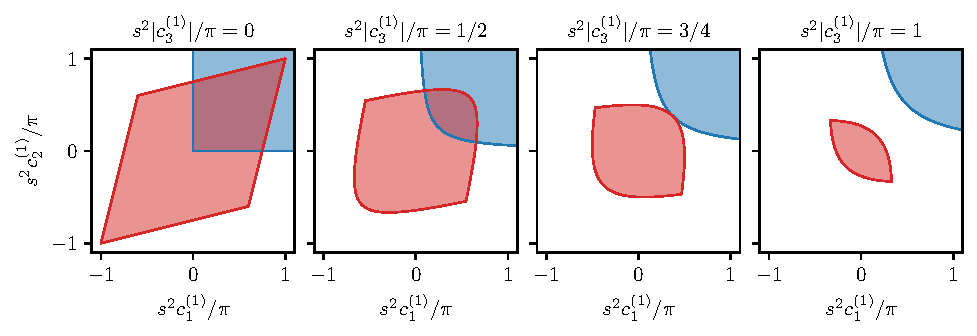
\includegraphics[width=\textwidth]{images/s1_plots_v3.pdf}
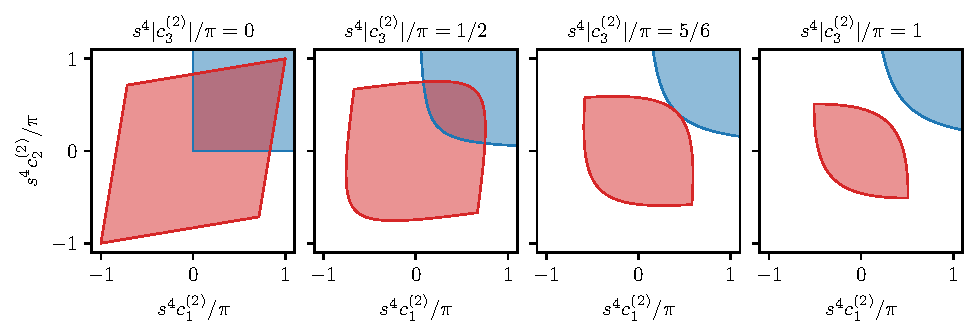
\includegraphics[width=\textwidth]{images/s2_plots_v3.pdf}
\caption{Regions allowed by partial-wave unitarity bounds (red, Eq.~\eqref{eq:PUbounds}) 
and positivity bounds (blue, Eq.~\eqref{eq:positivitybounds}) for the Euler-Heisenberg EFT
(upper panel, $S=1$) and the EFT of gravity (lower panel, $S=2$), in the
$(s^{2S}c_{1}^{(S)},s^{2S}c_{2}^{(S)})$ plane for different values of $s^{2S}c_3^{(S)}$.
\label{fig:s1}}
\end{figure}

\begin{figure}[tb]
    \centering
    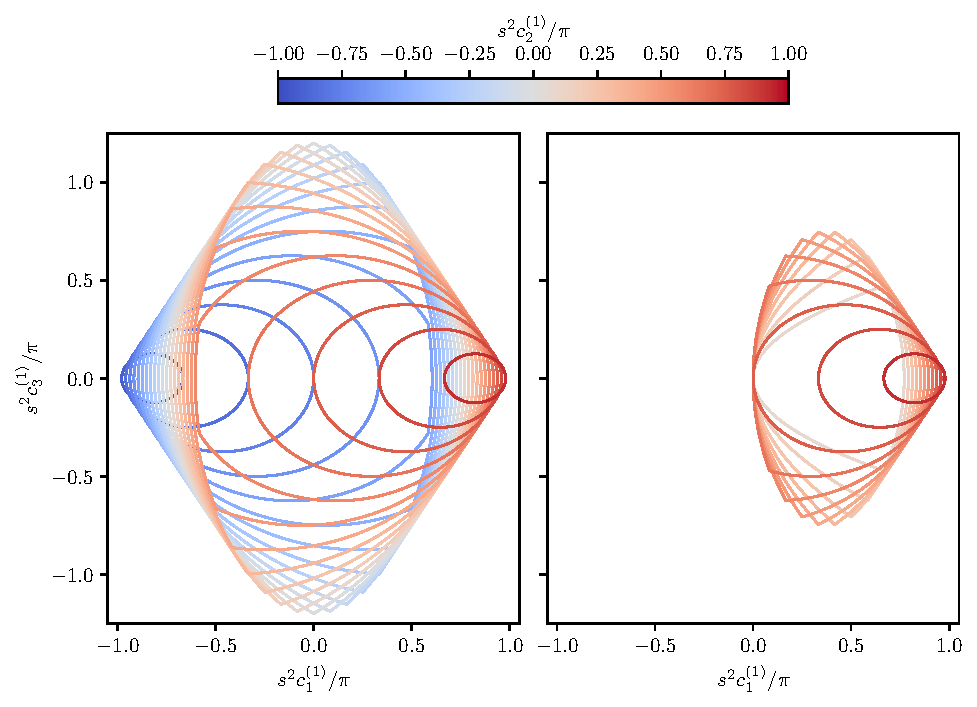
\includegraphics[scale = 0.90]{images/s1_plots_v2.pdf}
    \caption{Contours of the regions allowed by the partial-wave unitarity bounds (left panel, Eq.~\eqref{eq:PUbounds}) combined with the positivity constraints (right panel, Eq.~\eqref{eq:positivitybounds}) for the Euler-Heisenberg EFT ($S=1$) in the $(s^{2}c_{1}^{(1)},s^{2}c_{3}^{(1)})$ plane and computed for different values of $s^{2}c_2^{(1)}$.}
    \label{fig:s1_v2}
\end{figure}

\begin{figure}[tb]
    \centering
    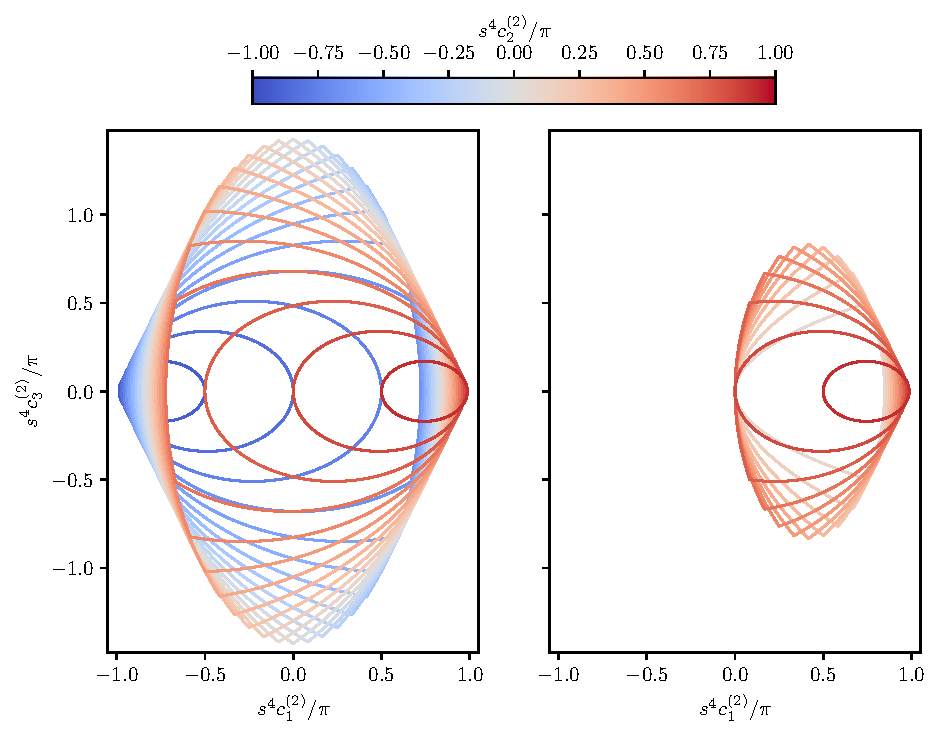
\includegraphics[scale = 0.90]{images/s2_plots_v2.pdf}
    \caption{Contours of the regions allowed by the partial-wave unitarity bounds (left panel, Eq.~\eqref{eq:PUbounds}) combined with the positivity constraints (right panel, Eq.~\eqref{eq:positivitybounds}) for the EFT of gravity ($S=2$) in the $(s^{4}c_{1}^{(2)},s^{4}c_{3}^{(2)})$ plane and computed for different values of $s^{4}c_2^{(2)}$.}
    \label{fig:s2_v2}
\end{figure}

Additional and complementary constraints on the EFT parameter space are represented by positivity bounds, which stem from the analyticity and causality of scattering amplitudes~\cite{Adams:2006sv}. In particular, they impose specific inequalities on the Wilson coefficients to ensure compatibility with a well-behaved UV completion.
%
In our scenarios, they read $\abs*{c_-^{(S)}} \le c_+^{(S)}$, or, equivalently,
%
\begin{align}
\label{eq:positivitybounds}
    \mathscr{P}: \qquad 
    c_{1,2}^{(S)} \ge 0 \,\,\,\,\,\text{and}\,\,\,\,\,
    (c_3^{(S)})^2 \le 4\, c_{1}^{(S)} c_{2}^{(S)}\,,
\end{align}
%
and are valid for both $S=1$~\cite{Adams:2006sv,Rebhan:2017zdx,Remmen:2019cyz,Henriksson:2021ymi,Arkani-Hamed:2020blm} 
and $S=2$~\cite{Gruzinov:2006ie,Bellazzini:2015cra,Endlich:2017tqa,Arkani-Hamed:2020blm,Caron-Huot:2022ugt,Bellazzini:2022wzv}.
%
The regions satisfying these positivity constraints are shown in blue in Figure~\ref{fig:s1} for the cases of $S=1,2$, and in the right panels of Figures \ref{fig:s1_v2} and \ref{fig:s2_v2}.
%The blue regions in Figure~\ref{fig:s1} satisfy positivity bounds. 
Interestingly, we emphasize that the viable parameter space is significantly reduced once both positivity and partial-wave unitarity bounds are imposed. 

To highlight the impact of positivity bounds, we compare the volume of the parameter space allowed by unitarity, $\text{Vol}(\mathscr U)$, with the one obtained after imposing the positivity constraints, $\text{Vol}(\mathscr U \cap \mathscr P)$.
In particular, for fixed values of the center-of-mass energy, we find
%
\begin{equation}
\frac{\text{Vol}(\mathscr U \cap \mathscr P)}{\text{Vol}(\mathscr U)} = \frac{1}{32}\left(\frac{2S+3}{S+1}\right)^{\!2}
    \approx 
    \begin{cases}
        0.20 & \text{for }S=1\,,\\
        0.17 & \text{for }S=2\,,
    \end{cases}
\end{equation}
%
which is a monotonically decreasing function of $S$.

\section{\texorpdfstring{$N \to M$ Scattering Amplitudes}{N-to-M Scattering Amplitudes}}

Another important advantage of our method over standard techniques 
is its capability of addressing partial-wave unitarity 
bounds for $N \to M$ scattering processes (with $N,M \geq 2$).

\subsection{Dimension-Six Example}

As an illustrative example, we consider the dimension-six 
SMEFT interactions~\cite{Grzadkowski:2010es}
\begin{align}
    \mathcal L^{(6)} \supset 
    C_{eH}^{pr}\left (H^\dagger H\right)\overline \ell_p e_r H + 
    C_{dH}^{pr}\left (H^\dagger H\right)\overline q_p d_r H  
     + C_{uH}^{pr}\left(H^\dagger H\right)\overline q_p u_r \widetilde H + \text{H.c.}
    \label{eq:SMEFT_6}
\end{align}
%
where $\widetilde H = i \sigma^2 H^*$ and $p,r$ are flavor indices.
As is well known, $\mathcal L^{(6)}$ induces modifications to the fermionic Yukawa couplings, which are a target of the High-Luminosity LHC program, and generates new contributions to multiboson interactions that might be probed at future colliders.

To obtain the corresponding unitarity bounds, we perform a coupled-channel analysis involving all possible contact amplitudes for
$\phi_a\phi_b \to \phi_c \psi_i^\pm\overline \psi_j^\pm$ and $\psi_i^\pm \overline\psi_j^\pm\to \phi_a\phi_b\phi_c$, where $\{\phi_a\}_{a=1}^4$ denote the real components of the Higgs doublet $H=(\phi_1+i\phi_3,\phi_2+i\phi_4)^T/\sqrt{2}$ and $\psi_i,\psi_j$ denote any Dirac fermions.
%
We find that the strongest unitarity bound arises from the $J=0$ partial waves and reads
%
\begin{equation}
\Tr[3\,C_{uH}C_{uH}^\dagger + 3\,C_{dH}C_{dH}^\dagger + C_{eH}C_{eH}^\dagger]  \le \left( \frac{ 32\pi^2}{\sqrt{3}s}\right)^2\,,\label{eq:SMEFTdim6UB}
\end{equation}
%
where the trace is understood over flavor indices.
%
As for the $\phi_a\phi_b \to \phi_c \overline \psi_i^+ \psi_j^+$ amplitude,
%
\begin{equation}
    \ket{\mathcal A_{1_{\phi_1},2_{\phi_1}\to 3_{\phi_1},4^+_{\overline \nu_p},5^+_{e_r}}} =
    \frac{3\sqrt{2}}{2}\left(C_{eH}^{pr}\right)^* \sqr{5}{4}\,,
\end{equation}
%
the relevant basis element of Appendix \ref{app:2-to-3_basis} is
%
\begin{align}
    \ket{\mathcal B^0_{1^0,2^0 \to 3^0,4^{\frac{1}{2}},5^{\frac{1}{2}}}} = \frac{32\sqrt{6}\pi^2}{s}\sqr{5}{4}\,,
\end{align}
%
where $s=(p_1+p_2)^2$. 
Therefore, without performing any phase-space integral,
we obtain the $J=0$ partial-wave coefficient
%
\begin{equation}
    a^0_{1_{\phi_1},2_{\phi_1}\to 3_{\phi_1},4^+_{\overline \nu_p},5^+_{e_r}} = \frac{\sqrt{3}s}{64\sqrt{2}\pi^2}\left(C_{eH}^{pr}\right)^*\,,
\end{equation}
%
where we included a $1/\sqrt{2}$ factor accounting for the identical particles in the initial state.

Instead, the unitarity bound stemming from $2 \to 2$ amplitudes, arising from Eq.~(\ref{eq:SMEFT_6}) by picking one vacuum expectation value $v$ out of a Higgs doublet, reads
%
\begin{equation}
 \Tr[3\,C_{uH}C_{uH}^\dagger + 3\,C_{dH}C_{dH}^\dagger + C_{eH}C_{eH}^\dagger]
    \le
    \frac{32\pi^2}{3 s v^2}
    \,,
\end{equation}
%
and is weaker than that of Eq.~\eqref{eq:SMEFTdim6UB} for $\sqrt{s} > 4 \pi v\sqrt{2}$.

\begin{figure}[tb]
\centering
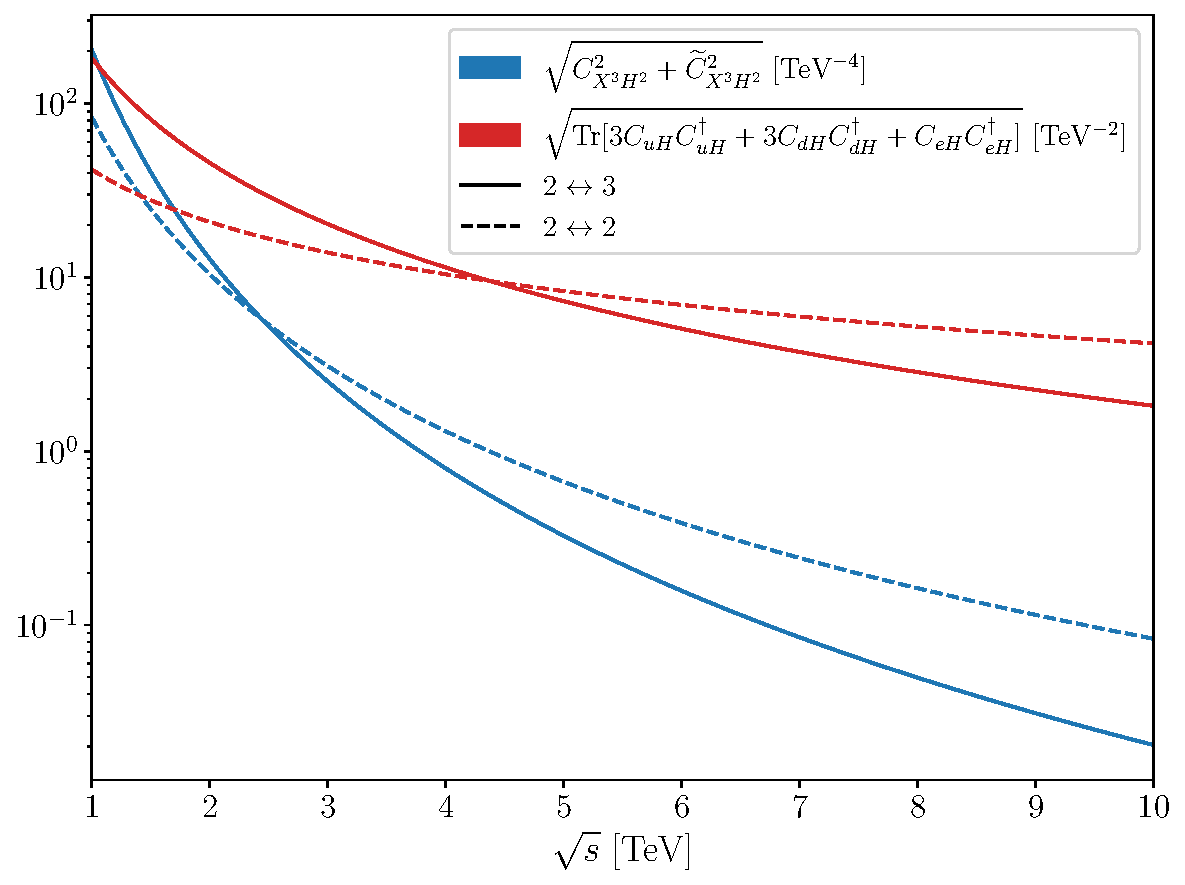
\includegraphics[width=0.8\textwidth]{images/SMEFT_plot_lin.pdf}
\caption{Partial-wave unitarity bounds on the Wilson coefficients of dimension-six (Eq.~\eqref{eq:SMEFT_6}) and dimension-eight (Eq.~\eqref{eq:SMEFT_8}) SMEFT operators
as functions of the center-of-mass energy $\sqrt{s}$ and stemming from
$2\to 2$ processes (dashed lines) and $2\to 3$ processes (solid lines).
$C_{X^3H^2}$ and $\widetilde C_{X^3H^2}$ refer to the gauge group $G=SU(3)$.}
\label{SMEFT_plot}
\end{figure}

\subsection{Dimension-Eight Example}

Next, we consider the following dimension-eight SMEFT interactions~\cite{Murphy:2020rsh}
%
\begin{align}
    \mathcal L^{(8)} \supset C_{X^3H^2}\left(H^\dagger H\right)f^{ABC}X^A_{\mu}{}^{\nu} X^B_{\nu}{}^{\rho} X^C_{\rho}{}^{\mu} + \widetilde C_{X^3H^2}\left(H^\dagger H\right)f^{ABC}X^A_{\mu}{}^{\nu} X^B_{\nu}{}^{\rho} \widetilde X^C_{\rho}{}^{\mu}\,,
    \label{eq:SMEFT_8}
\end{align}
%
where $X^A_{\mu\nu}$ is the field-strength tensor associated with a generic non-Abelian gauge group $G$ and $\widetilde X^A_{\mu\nu} = \frac{1}{2}\epsilon_{\mu\nu\rho\sigma}X^{A}{}^{\rho\sigma}$ is its dual.
%
The strongest unitarity constraint stems from the $J=0$ partial waves and reads
%
\begin{equation}
    C_{X^3H^2}^2+\widetilde C_{X^3H^2}^2 \le
    \left(\frac{32 \sqrt{10} \pi^2}{s^2}\right)^2 \frac{1}{C_2(G)\, d(G)}\,, 
    \label{eq:dim8unbroken}
\end{equation}
%
where $C_2(G)$ is the quadratic Casimir of the adjoint representation of $G$ and $d(G)$ is its dimension.\footnote{$C_2(G)$ is defined by $f^{ACD}f^{BCD} = C_2(G)\delta^{AB}$.
In particular, the structure constants of the $SU(N)$ group, which has dimension 
$d(SU(N)) = N^2 -1$, are normalized such that $C_2(SU(N)) = N$.}
This bound is obtained via a coupled-channel analysis that includes all the processes $\phi_a \phi_b \to X^A{}^\pm X^B{}^\pm X^C{}^\pm$. 
%
Taking the related amplitudes 
%
\begin{align}
    \ket{\mathcal A_{1_{\phi_a},2_{\phi_b} \to 3_{X^A}^-,4_{X^B}^-,5_{X^C}^-}} &= 
    3\sqrt{2}\left(iC_{X^3H^2}-\widetilde C_{X^3H^2}\right)\delta_{ab}  f^{ABC} \agl{3}{4}\agl{4}{5}\agl{3}{5}\,, \\
    \ket{\mathcal A_{1_{\phi_a},2_{\phi_b} \to 3_{X^A}^+,4_{X^B}^+,5_{X^C}^+}} &= 
    3\sqrt{2}\left(iC_{X^3H^2}+\widetilde C_{X^3H^2}\right)\delta_{ab}  f^{ABC} \sqr{4}{3}\sqr{5}{4}\sqr{5}{3}\,,
\end{align}
%
and the relevant vector basis element of Appendix \ref{app:2-to-3_basis}
%
\begin{equation}
    \ket{\mathcal B^0_{1^0,2^0 \to 3^1,4^{1},5^{1}}} = \frac{64\sqrt{30}\pi^2}{s^2}\sqr{4}{3}\sqr{5}{3}\sqr{5}{4}\,,
\end{equation}
%
we can immediately obtain the partial-wave coefficients by including the $1/\sqrt{2}$ symmetry factor:
\begin{align}
    a^0_{1_{\phi_a},2_{\phi_b} \to 
    3_{X^{A}}^\pm,4_{X^{B}}^\pm,5_{X^{C}}^\pm} =
    \frac{3 s^2 }{64\sqrt{30}\pi^2}\delta_{ab}f^{ABC}\left(iC_{X^3H^2}\pm \widetilde C_{X^3H^2}\right)
    \,.
\end{align}

Instead, $h X^A{}^\mp \to X^B{}^\pm X^C{}^\pm$ (corresponding to $J=1$) are the only available $2\to 2$ channels, and the related unitarity bound is
%
\begin{equation}
    C_{X^3H^2}^2+\widetilde C_{X^3H^2}^2 \le 
    %\left(\frac{8\sqrt{2}\pi}{v s^{3/2}}\right)^2 
    \frac{128\pi^2}{s^3 v^2}
    \frac{1}{C_2(G)}\,,
\end{equation}
which is weaker than that of Eq.~\eqref{eq:dim8unbroken} for $\sqrt{s} > 4\pi v\sqrt{5/d(G)}$.

In Figure~\ref{SMEFT_plot}, we show the unitarity bounds 
arising from $2\to 2$ and $2\to 3$ scattering processes as induced 
by $\mathcal L^{(6)}$ and $\mathcal L^{(8)}$; see 
Eqs.~\eqref{eq:SMEFT_6} and \eqref{eq:SMEFT_8}.

\section{Conclusions}

\begin{subappendices}
\section{\texorpdfstring{Angular-Momentum Basis for $2 \to 3$ Amplitudes}{Angular-Momentum Basis for 2-to-3 Amplitudes}\label{app:2-to-3_basis}}

In this appendix we list the normalized kinematic polynomials with definite angular momentum $J_{12}$ relevant for $2 \to 3$ helicity amplitudes, obtained by following the algorithm presented in Section~\ref{sec:PWUB_formalism}.
They are denoted by $\ket*{\mathcal B^{J_{12}}_{i\to f}}$, where $i=(1^{-h_1},2^{-h_2})$ and $f=(3^{h_3},4^{h_4},5^{h_5})$, while $s_{12} = (p_1+p_2)^2$.
They are reported in Table~\ref{tab:2to3basis}.
We report only those with $\sum_{i=1}^5 h_i \ge 0$. The helicity configurations not listed here can be recovered from those reported
by applying a parity flip, i.e., by performing the following substitutions: $h_i \to -h_i$ and $\agl{i}{j}\leftrightarrow \sqr{j}{i}$ for all $i,j$.
Notice that, in many cases, the reported subspace of $V_{i\to f}$ with fixed angular momentum is degenerate.
This degeneracy is due to the fact that a subset of particles in the final state can have more than one angular momentum value.

\begin{comment}
\begin{eqnarray*}
    %\toprule
    \toprule
    (h_1,h_2;h_3,h_4,h_5) &
    %\,\,\,\,\, 
    \qquad\qquad
    J_{12}
    %\,\,\,\,\, 
    \qquad\qquad
    & \ket*{\mathcal B^{J_{12}}_{i \to f}}\\ 
    %\midrule
    \midrule
    (-1,-1;0,1,1) & 0 & 64\sqrt{3}\pi^2s_{12}^{-5/2} \agl{1}{2}^2 \sqr{5}{4}^2 \\
    (-1,-1;\hf,\hf,1) & 0 & 64\sqrt{6}\pi^2s_{12}^{-5/2} \agl{1}{2}^2 \sqr{5}{3}\sqr{5}{4} \\
    (-1,-1;1,1,1) & 0 & 64\sqrt{30}\pi^2s_{12}^{-3} \agl{1}{2}^2 \sqr{4}{3}\sqr{5}{3} \sqr{5}{4} \\
    \hline
    (-1,-\hf;-\hf,1,1) & \hf & 64\sqrt{30}\pi^2s_{12}^{-5/2} \agl{1}{2}\agl{1}{3}\sqr{5}{4}^2 \\
    (-1,-\hf;0,\hf,1) & \hf & 64\sqrt{15}\pi^2s_{12}^{-5/2} \agl{1}{2}\agl{1}{4}\sqr{5}{4}^2 \\
    && 128\sqrt{10}\pi^2s_{12}^{-5/2} \agl{1}{2}\agl{1}{3}\sqr{5}{3}\sqr{5}{4} \\
    (-1,-\hf;\hf,\hf,\hf) & \hf & 64\sqrt{30}\pi^2s_{12}^{-5/2} \agl{1}{2}\agl{1}{3}\sqr{4}{3}\sqr{5}{3} \\
    && 64\sqrt{30}\pi^2s_{12}^{-5/2} \agl{1}{2}\agl{1}{4}\sqr{4}{3}\sqr{5}{4} \\
    && 64\sqrt{30}\pi^2s_{12}^{-5/2} \agl{1}{2}\agl{1}{5}\sqr{5}{3}\sqr{5}{4} \\
    (-1,-\hf;\hf,1,1) & \hf & 384\sqrt{2}\pi^2s_{12}^{-3} \agl{1}{2}\agl{1}{4}\sqr{4}{3}\sqr{5}{4}^2 \\
    && 384\sqrt{2}\pi^2s_{12}^{-3} \agl{1}{2}\agl{1}{5}\sqr{5}{3}\sqr{5}{4}^2 \\
    && 384\sqrt{5}\pi^2s_{12}^{-3} \agl{1}{2}\agl{1}{3}\sqr{4}{3}\sqr{5}{3}\sqr{5}{4} \\
    \hline
    (-1,0;-1,1,1) & 1 & 192\sqrt{15}\pi^2 s_{12}^{-5/2}\agl{1}{3}^2 \sqr{5}{4}^2\\
    (-1,0;-\hf,\hf,1) & 1 & 192\sqrt{15}\pi^2 s_{12}^{-5/2}\agl{1}{3}^2 \sqr{5}{3} \sqr{5}{4} \\
    && 192\sqrt{15}\pi^2 s_{12}^{-5/2}\agl{1}{3}\agl{1}{4} \sqr{5}{4}^2 \\
    (-1,0;0,0,1) & 1 & 288\sqrt{2}\pi^2s_{12}^{-5/2}\agl{1}{4}^2\sqr{5}{4}^2  \\
    && 288\sqrt{2}\pi^2s_{12}^{-5/2}\agl{1}{3}^2\sqr{5}{3}^2 \\
    && 1152\sqrt{\tfrac{5}{7}}\pi^2s_{12}^{-5/2}\agl{1}{3}\agl{1}{4}\sqr{5}{3}\sqr{5}{4} \\
    (-1,0;0,\hf,\hf) & 1 & 576\pi^2 s_{12}^{-5/2}\agl{1}{4}\agl{1}{5}\sqr{5}{4}^2 \\
    && 576\pi^2 s_{12}^{-5/2}\agl{1}{3}^2\sqr{4}{3}\sqr{5}{3} \\
    && 288\sqrt{10}\pi^2 s_{12}^{-5/2}\agl{1}{3}\agl{1}{5}\sqr{5}{3}\sqr{5}{4} \\
    && 288\sqrt{10}\pi^2 s_{12}^{-5/2}\agl{1}{3}\agl{1}{4}\sqr{4}{3}\sqr{5}{4} \\
    (-1,0;0,1,1) & 1 & 192\sqrt{14}\pi^2s_{12}^{-3}\agl{1}{4}\agl{1}{5}\sqr{5}{4}^3 \\
    && 576\sqrt{7}\pi^2s_{12}^{-3}\agl{1}{3}\agl{1}{5}\sqr{5}{3}\sqr{5}{4}^2 \\
    && 576\sqrt{7}\pi^2s_{12}^{-3}\agl{1}{3}\agl{1}{4}\sqr{4}{3}\sqr{5}{4}^2 \\
    && 576\sqrt{7}\pi^2s_{12}^{-3}\agl{1}{3}^2\sqr{4}{3}\sqr{5}{3}\sqr{5}{4} \\
    (-1,0;\hf,\hf,1) & 1 & 192\sqrt{21}\pi^2s_{12}^{-3}\agl{1}{4}^2\sqr{4}{3}\sqr{5}{4}^2 \\
    && 192\sqrt{21}\pi^2s_{12}^{-3}\agl{1}{3}^2\sqr{4}{3}\sqr{5}{3}^2 \\
    && 1152\sqrt{\tfrac{7}{5}}\pi^2s_{12}^{-3}\agl{1}{4}\agl{1}{5}\sqr{5}{3}\sqr{5}{4}^2\\
    && 1152\sqrt{\tfrac{7}{5}}\pi^2s_{12}^{-3}\agl{1}{3}\agl{1}{5}\sqr{5}{3}^2\sqr{5}{4} \\
    && 1152\sqrt{\tfrac{35}{11}}\pi^2s_{12}^{-3}\agl{1}{3}\agl{1}{4}\sqr{4}{3}\sqr{5}{3}\sqr{5}{4} \\
    (-1,0;1,1,1) & 1 & 384\sqrt{15}\pi^2s_{12}^{-7/2} \agl{1}{5}^2\sqr{5}{3}^2 \sqr{5}{4}^2 \\
    && 384\sqrt{15}\pi^2s_{12}^{-7/2} \agl{1}{4}^2\sqr{4}{3}^2 \sqr{5}{4}^2 \\
    && 384\sqrt{15}\pi^2s_{12}^{-7/2} \agl{1}{3}^2\sqr{4}{3}^2 \sqr{5}{3}^2 \\
    && 576\sqrt{35}\pi^2s_{12}^{-7/2} \agl{1}{4}\agl{1}{5}\sqr{4}{3} \sqr{5}{3}\sqr{5}{4}^2 \\
    && 576\sqrt{35}\pi^2s_{12}^{-7/2} \agl{1}{3}\agl{1}{5}\sqr{4}{3} \sqr{5}{3}^2\sqr{5}{4} \\
    && 576\sqrt{35}\pi^2s_{12}^{-7/2} \agl{1}{3}\agl{1}{4}\sqr{4}{3}^2 \sqr{5}{3}\sqr{5}{4} \\
    \hline
    (-1,\hf;-1,\hf,1) & \tfrac{3}{2} & 768\pi^2s_{12}^{-5/2} \agl{1}{3}^2\sqr{5}{2}\sqr{5}{4} \\
    (-1,\hf;-\hf,0,1) & \tfrac{3}{2} & 768\sqrt{\tfrac{15}{37}}\pi^2s_{12}^{-5/2} \agl{1}{3}^2\sqr{5}{2}\sqr{5}{3} \\
    && 768\sqrt{\tfrac{15}{13}}\pi^2s_{12}^{-5/2} \agl{1}{3}\agl{1}{4}\sqr{5}{2}\sqr{5}{4} \\
    (-1,\hf;-\hf,\hf,\hf) & \tfrac{3}{2} & 384\sqrt{3}\pi^2s_{12}^{-5/2} \agl{1}{3}^2\sqr{4}{2}\sqr{5}{3} \\
    && 192\sqrt{30}\pi^2s_{12}^{-5/2} \agl{1}{3}\agl{1}{5}\sqr{5}{2}\sqr{5}{4} \\
    && 192\sqrt{30}\pi^2s_{12}^{-5/2} \agl{1}{3}\agl{1}{4}\sqr{4}{2}\sqr{5}{4} \\
    (-1,\hf;-\hf,1,1) & \tfrac{3}{2} & 768\sqrt{\tfrac{21}{5}}\pi^2s_{12}^{-3} \agl{1}{3}^2\sqr{4}{2}\sqr{5}{3}\sqr{5}{4} \\
    && 768\sqrt{\tfrac{21}{5}}\pi^2s_{12}^{-3} \agl{1}{3}\agl{1}{5}\sqr{5}{2}\sqr{5}{4}^2 \\
    && 768\sqrt{\tfrac{21}{5}}\pi^2s_{12}^{-3} \agl{1}{3}\agl{1}{4}\sqr{4}{2}\sqr{5}{4}^2 \\
    (-1,\hf;0,0,\hf) & \tfrac{3}{2} & 768\pi^2s_{12}^{-5/2} \agl{1}{4}^2\sqr{4}{2}\sqr{5}{4} \\
    && 768\sqrt{\tfrac{15}{13}}\pi^2s_{12}^{-5/2} \agl{1}{3}\agl{1}{5}\sqr{5}{2}\sqr{5}{3} \\
    && 768\sqrt{\tfrac{15}{13}}\pi^2s_{12}^{-5/2} \agl{1}{4}\agl{1}{5}\sqr{5}{2}\sqr{5}{4} \\
    && 384\sqrt{10}\pi^2s_{12}^{-5/2} \agl{1}{3}\agl{1}{4}\sqr{4}{2}\sqr{5}{3} \\
    (-1,\hf;0,\hf,1) & \tfrac{3}{2} & 384\sqrt{7}\pi^2s_{12}^{-3} \agl{1}{3}^2\sqr{4}{2}\sqr{5}{3}^2 \\
    && 384\sqrt{7}\pi^2s_{12}^{-3} \agl{1}{4}^2\sqr{4}{2}\sqr{5}{4}^2 \\
    && 768\sqrt{\tfrac{21}{11}}\pi^2s_{12}^{-3} \agl{1}{4}\agl{1}{5}\sqr{5}{2}\sqr{5}{4}^2 \\
    && 384\sqrt{21}\pi^2s_{12}^{-3} \agl{1}{3}\agl{1}{5}\sqr{5}{2}\sqr{5}{3}\sqr{5}{4} \\
    && 768\sqrt{\tfrac{105}{11}}\pi^2s_{12}^{-3} \agl{1}{3}\agl{1}{4}\sqr{4}{2}\sqr{5}{3}\sqr{5}{4} \\
    (-1,\hf;\hf,\hf,\hf) & \tfrac{3}{2} & 384\sqrt{14}\pi^2s_{12}^{-3} \agl{1}{4}^2\sqr{4}{2}\sqr{4}{3}\sqr{5}{4} \\
    && 384\sqrt{14}\pi^2s_{12}^{-3} \agl{1}{5}^2\sqr{5}{2}\sqr{5}{3}\sqr{5}{4} \\
    && 384\sqrt{14}\pi^2s_{12}^{-3} \agl{1}{3}\agl{1}{5}\sqr{4}{2}\sqr{5}{3}^2 \\
    && 384\sqrt{14}\pi^2s_{12}^{-3} \agl{1}{4}\agl{1}{5}\sqr{3}{2}\sqr{5}{4}^2 \\
    && 192\sqrt{105}\pi^2s_{12}^{-3} \agl{1}{3}\agl{1}{4}\sqr{4}{2}\sqr{4}{3}\sqr{5}{3} \\
    && 192\sqrt{105}\pi^2s_{12}^{-3} \agl{1}{4}\agl{1}{5}\sqr{4}{2}\sqr{5}{3}\sqr{5}{4} \\
    (-1,\hf;\hf,1,1) & \tfrac{3}{2} & 512\sqrt{\tfrac{210}{17}}\pi^2s_{12}^{-7/2} \agl{1}{3}^2\sqr{4}{2}\sqr{4}{3}\sqr{5}{3}^2 \\
    && 512\sqrt{15}\pi^2s_{12}^{-7/2} \agl{1}{4}\agl{1}{5}\sqr{3}{2}\sqr{5}{4}^3 \\
    && 1536\sqrt{2}\pi^2s_{12}^{-7/2} \agl{1}{5}^2\sqr{5}{2}\sqr{5}{3}\sqr{5}{4}^2 \\
    && 1536\sqrt{2}\pi^2s_{12}^{-7/2} \agl{1}{4}^2\sqr{4}{2}\sqr{4}{3}\sqr{5}{4}^2 \\
    && 1536\sqrt{\tfrac{42}{13}}\pi^2s_{12}^{-7/2} \agl{1}{4}\agl{1}{5}\sqr{4}{2}\sqr{5}{3}\sqr{5}{4}^2 \\
    && 1536\sqrt{\tfrac{70}{19}}\pi^2s_{12}^{-7/2} \agl{1}{3}\agl{1}{5}\sqr{4}{2}\sqr{5}{3}^2\sqr{5}{4} \\
    && 1536\sqrt{\tfrac{42}{5}}\pi^2s_{12}^{-7/2} \agl{1}{3}\agl{1}{4}\sqr{4}{2}\sqr{4}{3}\sqr{5}{3}\sqr{5}{4}\\
    \hline
    (-1,1;-1,0,1) & 2 & 96\sqrt{30}\pi^2s_{12}^{-5/2} \agl{1}{3}^2\sqr{5}{2}^2 \\
    (-1,1;-1,\hf,\hf) & 2 & 192\sqrt{15}\pi^2s_{12}^{-5/2} \agl{1}{3}^2\sqr{4}{2}\sqr{5}{2} \\
    (-1,1;-1,1,1) & 2 & 192\sqrt{70}\pi^2s_{12}^{-3} \agl{1}{3}^2\sqr{4}{2}\sqr{5}{2}\sqr{5}{4} \\
    (-1,1;-\hf,0,\hf) & 2 & 960\pi^2s_{12}^{-5/2} \agl{1}{3}\agl{1}{5}\sqr{5}{2}^2 \\
    && 480\sqrt{6}\pi^2s_{12}^{-5/2} \agl{1}{3}\agl{1}{4}\sqr{4}{2}\sqr{5}{2} \\
    (-1,1;-\hf,\hf,1) & 2 & 384\sqrt{\tfrac{105}{11}}\pi^2s_{12}^{-3} \agl{1}{3}^2\sqr{4}{2}\sqr{5}{2}\sqr{5}{3} \\
    && 384\sqrt{21}\pi^2s_{12}^{-3} \agl{1}{3}\agl{1}{5}\sqr{5}{2}^2\sqr{5}{4} \\
    && 192\sqrt{105}\pi^2s_{12}^{-3} \agl{1}{3}\agl{1}{4}\sqr{4}{2}\sqr{5}{2}\sqr{5}{4} \\
    (-1,1;0,0,0) & 2 & 960\pi^2s_{12}^{-5/2} \agl{1}{5}^2\sqr{5}{2}^2 \\
    && 960\pi^2s_{12}^{-5/2} \agl{1}{4}^2\sqr{4}{2}^2 \\
    && 1920\sqrt{\tfrac{3}{7}}\pi^2s_{12}^{-5/2} \agl{1}{4}\agl{1}{5}\sqr{4}{2}\sqr{5}{2} \\
    (-1,1;0,0,1) & 2 & 960\sqrt{\tfrac{21}{11}}\pi^2s_{12}^{-3} \agl{1}{3}\agl{1}{5}\sqr{5}{2}^2\sqr{5}{3} \\
    && 960\sqrt{\tfrac{21}{11}}\pi^2s_{12}^{-3} \agl{1}{4}\agl{1}{5}\sqr{5}{2}^2\sqr{5}{4} \\
    && 960\sqrt{\tfrac{21}{11}}\pi^2s_{12}^{-3} \agl{1}{4}^2\sqr{4}{2}\sqr{5}{2}\sqr{5}{4} \\
    && 480\sqrt{21}\pi^2s_{12}^{-3} \agl{1}{3}\agl{1}{4}\sqr{4}{2}\sqr{5}{2}\sqr{5}{3} \\
    (-1,1;0,\hf,\hf) & 2 & 320\sqrt{21}\pi^2s_{12}^{-3} \agl{1}{5}^2\sqr{5}{2}^2\sqr{5}{4} \\
    && 320\sqrt{21}\pi^2s_{12}^{-3} \agl{1}{4}^2\sqr{4}{2}^2\sqr{5}{4} \\
    && 384\sqrt{35}\pi^2s_{12}^{-3} \agl{1}{3}\agl{1}{4}\sqr{4}{2}^2\sqr{5}{3} \\
    && 192\sqrt{105}\pi^2s_{12}^{-3} \agl{1}{3}\agl{1}{5}\sqr{4}{2}\sqr{5}{2}\sqr{5}{3} \\
    && 640\sqrt{7}\pi^2s_{12}^{-3} \agl{1}{4}\agl{1}{5}\sqr{4}{2}\sqr{5}{2}\sqr{5}{4} \\
    (-1,1;0,1,1) & 2 & 1920\pi^2s_{12}^{-7/2} \agl{1}{3}^2\sqr{4}{2}^2\sqr{5}{3}^2 \\
    && 1920\pi^2s_{12}^{-7/2} \agl{1}{5}^2\sqr{5}{2}^2\sqr{5}{4}^2 \\
    && 1920\pi^2s_{12}^{-7/2} \agl{1}{4}^2\sqr{4}{2}^2\sqr{5}{4}^2 \\
    && 960\sqrt{21}\pi^2s_{12}^{-7/2} \agl{1}{3}\agl{1}{4}\sqr{4}{2}^2\sqr{5}{3}\sqr{5}{4}\\
    && 384\sqrt{30}\pi^2s_{12}^{-7/2} \agl{1}{4}\agl{1}{5}\sqr{4}{2}\sqr{5}{2}\sqr{5}{4}^2 \\
    && 1920\sqrt{\tfrac{42}{11}}\pi^2s_{12}^{-7/2} \agl{1}{3}\agl{1}{5}\sqr{4}{2}\sqr{5}{2}\sqr{5}{3}\sqr{5}{4} \\
    (-1,1;\hf,\hf,1) & 2 & 640\sqrt{42}\pi^2s_{12}^{-7/2} \agl{1}{3}\agl{1}{4}\sqr{4}{2}^2\sqr{5}{3}^2 \\
    && 640\sqrt{42}\pi^2s_{12}^{-7/2} \agl{1}{4}^2\sqr{4}{2}^2\sqr{5}{3}\sqr{5}{4} \\
    && 256\sqrt{105}\pi^2s_{12}^{-7/2} \agl{1}{4}^2\sqr{3}{2}\sqr{4}{2}\sqr{5}{4}^2 \\
    && 1920\sqrt{2}\pi^2s_{12}^{-7/2} \agl{1}{5}^2\sqr{5}{2}^2\sqr{5}{3}\sqr{5}{4} \\
    && 3840\sqrt{\tfrac{7}{13}}\pi^2s_{12}^{-7/2} \agl{1}{3}\agl{1}{5}\sqr{4}{2}\sqr{5}{2}\sqr{5}{3}^2 \\
    && 3840\sqrt{\tfrac{7}{13}}\pi^2s_{12}^{-7/2} \agl{1}{4}\agl{1}{5}\sqr{3}{2}\sqr{5}{2}\sqr{5}{4}^2 \\
    && 3840\sqrt{\tfrac{21}{19}}\pi^2s_{12}^{-7/2} \agl{1}{4}\agl{1}{5}\sqr{4}{2}\sqr{5}{2}\sqr{5}{3}\sqr{5}{4} \\
    (-1,1;1,1,1) & 2 & 288\sqrt{2}\pi^2s_{12}^{-4} \agl{1}{3}\agl{1}{5}\sqr{4}{2}^2\sqr{5}{3}^3 \\
    && 288\sqrt{2}\pi^2s_{12}^{-4} \agl{1}{4}\agl{1}{5}\sqr{3}{2}^2\sqr{5}{4}^3 \\
    && 1152\sqrt{35}\pi^2s_{12}^{-4} \agl{1}{3}\agl{1}{4}\sqr{4}{2}^2\sqr{4}{3}\sqr{5}{3}^2 \\
    && 1152\sqrt{35}\pi^2s_{12}^{-4} \agl{1}{4}\agl{1}{5}\sqr{4}{2}^2\sqr{5}{3}^2\sqr{5}{4} \\
    && 5760\sqrt{2}\pi^2s_{12}^{-4} \agl{1}{4}^2\sqr{4}{2}^2\sqr{4}{3}\sqr{5}{3}\sqr{5}{4} \\
    && 1920\sqrt{6}\pi^2s_{12}^{-4} \agl{1}{4}^2\sqr{3}{2}\sqr{4}{2}\sqr{4}{3}\sqr{5}{4}^2 \\
    && 1920\sqrt{6}\pi^2s_{12}^{-4} \agl{1}{5}^2\sqr{3}{2}\sqr{5}{2}\sqr{5}{3}\sqr{5}{4}^2 \\
    && 1920\sqrt{6}\pi^2s_{12}^{-4} \agl{1}{5}^2\sqr{4}{2}\sqr{5}{2}\sqr{5}{3}^2\sqr{5}{4} \\
    && 960\sqrt{42}\pi^2s_{12}^{-4} \agl{1}{4}\agl{1}{5}\sqr{3}{2}\sqr{4}{2}\sqr{5}{3}\sqr{5}{4}^2 \\
    \hline
    (-\hf,-\hf;-1,1,1) & 1 & 192\sqrt{30}\pi^2s_{12}^{-5/2} \agl{1}{3}\agl{2}{3}\sqr{5}{4}^2 \\
    (-\hf,-\hf;-\hf,\hf,1) & 0 & 64\sqrt{15}\pi^2s_{12}^{-5/2} \agl{1}{2}\agl{3}{4}\sqr{5}{4}^2 \\
    (-\hf,-\hf;0,0,1) & 0 & 64\sqrt{30}\pi^2s_{12}^{-5/2} \agl{1}{2}\agl{3}{4}\sqr{5}{3}\sqr{5}{4} \\
    (-\hf,-\hf;0,\hf,\hf) & 0 & 32\sqrt{6}\pi^2s_{12}^{-3/2} \agl{1}{2}\sqr{5}{4} \\
    (-\hf,-\hf;0,1,1) & 0 & 64\sqrt{3}\pi^2s_{12}^{-2} \agl{1}{2}\sqr{5}{4}^2 \\
    (-\hf,-\hf;\hf,\hf,1) & 0 & 64\sqrt{6}\pi^2s_{12}^{-2} \agl{1}{2}\sqr{5}{3}\sqr{5}{4} \\
    (-\hf,-\hf;1,1,1) & 0 & 64\sqrt{30}\pi^2s_{12}^{-5/2} \agl{1}{2}\sqr{4}{3}\sqr{5}{3}\sqr{5}{4} \\
    \hline
    (-\tfrac{1}{2},0;-1,\tfrac{1}{2},1) & \tfrac{1}{2} & 128\sqrt{30}\pi^2 s_{12}^{-5/2}\agl{1}{3}\agl{3}{4}\sqr{5}{4}^2 \\
    (-\tfrac{1}{2},0;-\tfrac{1}{2},0,1) & \tfrac{1}{2} & 384\sqrt{5}\pi^2 s_{12}^{-5/2} \agl{1}{3}\agl{3}{4}\sqr{5}{3}\sqr{5}{4} \\
    && 128\sqrt{10}\pi^2 s_{12}^{-5/2} \agl{1}{2}\agl{3}{4}\sqr{5}{2}\sqr{5}{4} \\
    (-\tfrac{1}{2},0;-\tfrac{1}{2},\tfrac{1}{2},\tfrac{1}{2}) & \tfrac{1}{2} & 128\sqrt{3}\pi^2 s_{12}^{-3/2}\agl{1}{3}\sqr{5}{4} \\
    (-\tfrac{1}{2},0;-\tfrac{1}{2},1,1) & \tfrac{1}{2} & 64\sqrt{30}\pi^2 s_{12}^{-2}\agl{1}{3}\sqr{5}{4}^2 \\
    (-\tfrac{1}{2},0;0,0,\tfrac{1}{2}) & \tfrac{1}{2} & 128\sqrt{2}\pi^2s_{12}^{-3/2}\agl{1}{3}\sqr{5}{3} \\
    && 128\sqrt{2}\pi^2s_{12}^{-3/2}\agl{1}{4}\sqr{5}{4}\\
    (-\tfrac{1}{2},0;0,\tfrac{1}{2},1) & \tfrac{1}{2} & 64\sqrt{15}\pi^2s_{12}^{-2}\agl{1}{4}\sqr{5}{4}^2 \\
    && 128\sqrt{10}\pi^2 s_{12}^{-2}\agl{1}{3}\sqr{5}{3} \sqr{5}{4} \\
    (-\tfrac{1}{2},0;\tfrac{1}{2},\tfrac{1}{2},\tfrac{1}{2}) & \tfrac{1}{2} & 64\sqrt{30}\pi^2 s_{12}^{-2} \agl{1}{3}\sqr{4}{3}\sqr{5}{3} \\
    && 64\sqrt{30}\pi^2 s_{12}^{-2} \agl{1}{4}\sqr{4}{3}\sqr{5}{4} \\
    && 64\sqrt{30}\pi^2 s_{12}^{-2} \agl{1}{5}\sqr{5}{3}\sqr{5}{4} \\
    (-\tfrac{1}{2},0;\tfrac{1}{2},1,1) & \tfrac{1}{2} & 384\sqrt{5}\pi^2 s_{12}^{-5/2} \agl{1}{3}\sqr{4}{3}\sqr{5}{3}\sqr{5}{4} \\
    && 384\sqrt{5}\pi^2 s_{12}^{-5/2} \agl{1}{4}\sqr{4}{3}\sqr{5}{4}^2 \\
    && 384\sqrt{5}\pi^2 s_{12}^{-5/2} \agl{1}{5}\sqr{5}{3}\sqr{5}{4}^2 \\
    \hline
    (-\hf,\hf;-1,0,1) & 1 & 288\sqrt{10}\pi^2s_{12}^{-5/2} \agl{1}{3}\agl{3}{4}\sqr{5}{2}\sqr{5}{4} \\
    (-\hf,\hf;-1,\hf,\hf) & 1 & 1152\sqrt{\tfrac{5}{13}}\pi^2s_{12}^{-5/2} \agl{1}{3}\agl{3}{5}\sqr{5}{2}\sqr{5}{4} \\
    && 1152\sqrt{\tfrac{5}{13}}\pi^2s_{12}^{-5/2} \agl{1}{3}\agl{3}{4}\sqr{4}{2}\sqr{5}{4} \\
    (-\hf,\hf;-1,1,1) & 1 & 1152\sqrt{\tfrac{35}{31}}\pi^2s_{12}^{-3} \agl{1}{3}\agl{3}{5}\sqr{5}{2}\sqr{5}{4}^2 \\
    && 1152\sqrt{\tfrac{35}{31}}\pi^2s_{12}^{-3} \agl{1}{3}\agl{3}{4}\sqr{4}{2}\sqr{5}{4}^2 \\
    (-\hf,\hf;-\hf,0,\hf) & 1 & 128\sqrt{3}\pi^2s_{12}^{-3/2} \agl{1}{3}\sqr{5}{2} \\
    (-\hf,\hf;-\hf,\hf,1) & 1 & 192\sqrt{5}\pi^2s_{12}^{-2} \agl{1}{3}\sqr{5}{2}\sqr{5}{4} \\
    (-\hf,\hf;0,0,0) & 1 & 192\sqrt{2}\pi^2s_{12}^{-3/2} \agl{1}{4}\sqr{4}{2} \\
    && 192\sqrt{2}\pi^2s_{12}^{-3/2} \agl{1}{5}\sqr{5}{2} \\
    (-\hf,\hf;0,0,1) & 1 & 384\sqrt{\tfrac{5}{7}}\pi^2s_{12}^{-2} \agl{1}{3}\sqr{5}{2}\sqr{5}{3} \\
    && 384\sqrt{\tfrac{5}{7}}\pi^2s_{12}^{-2} \agl{1}{4}\sqr{5}{2}\sqr{5}{4} \\
    (-\hf,\hf;0,\hf,\hf) & 1 & 192\sqrt{5}\pi^2s_{12}^{-2} \agl{1}{3}\sqr{4}{2}\sqr{5}{3} \\
    && 192\sqrt{5}\pi^2s_{12}^{-2} \agl{1}{4}\sqr{4}{2}\sqr{5}{4} \\
    && 192\sqrt{5}\pi^2s_{12}^{-2} \agl{1}{5}\sqr{5}{2}\sqr{5}{4}  \\
    (-\hf,\hf;0,1,1) & 1 & 576\pi^2s_{12}^{-5/2} \agl{1}{5}\sqr{5}{2}\sqr{5}{4}^2  \\
    && 576\pi^2s_{12}^{-5/2} \agl{1}{4}\sqr{4}{2}\sqr{5}{4}^2 \\
    && 288\sqrt{10}\pi^2s_{12}^{-5/2} \agl{1}{3}\sqr{4}{2}\sqr{5}{3}\sqr{5}{4} \\
    (-\hf,\hf;\hf,\hf,1) & 1 & 384\sqrt{3}\pi^2s_{12}^{-5/2} \agl{1}{4}\sqr{3}{2}\sqr{5}{4}^2 \\
    && 384\sqrt{3}\pi^2s_{12}^{-5/2} \agl{1}{3}\sqr{4}{2}\sqr{5}{3}^2 \\
    && 576\sqrt{2}\pi^2s_{12}^{-5/2} \agl{1}{5}\sqr{5}{2}\sqr{5}{3}\sqr{5}{4} \\
    && 192\sqrt{30}\pi^2s_{12}^{-5/2} \agl{1}{4}\sqr{4}{2}\sqr{5}{3}\sqr{5}{4} \\
    (-\hf,\hf;1,1,1) & 1 & 1152\sqrt{\tfrac{35}{31}}\pi^2s_{12}^{-3} \agl{1}{4}\sqr{3}{2}\sqr{4}{3}\sqr{5}{4}^2 \\
    && 1152\sqrt{\tfrac{35}{31}}\pi^2s_{12}^{-3} \agl{1}{5}\sqr{3}{2}\sqr{5}{3}\sqr{5}{4}^2 \\
    && 1152\sqrt{\tfrac{35}{31}}\pi^2s_{12}^{-3} \agl{1}{3}\sqr{4}{2}\sqr{4}{3}\sqr{5}{3}^2 \\
    && 1152\sqrt{\tfrac{35}{31}}\pi^2s_{12}^{-3} \agl{1}{5}\sqr{4}{2}\sqr{5}{3}^2\sqr{5}{4} \\
    && 576\sqrt{14}\pi^2s_{12}^{-3} \agl{1}{4}\sqr{4}{2}\sqr{4}{3}\sqr{5}{3}\sqr{5}{4} \\
    \hline
    (-\hf,1;-1,\hf,1) & \tfrac{3}{2} & 768\sqrt{\tfrac{21}{11}}\pi^2s_{12}^{-3} \agl{1}{3}\agl{3}{5}\sqr{5}{2}^2\sqr{5}{4}\\
    && 384\sqrt{21}\pi^2s_{12}^{-3} \agl{1}{3}\agl{3}{4}\sqr{4}{2}\sqr{5}{2}\sqr{5}{4} \\
    (-\hf,1;-\hf,0,1) & \tfrac{3}{2} & 64\sqrt{30}\pi^2s_{12}^{-2} \agl{1}{3}\sqr{5}{2}^2 \\
    (-\hf,1;-\hf,\hf,\hf) & \tfrac{3}{2} & 128\sqrt{15}\pi^2s_{12}^{-2} \agl{1}{3}\sqr{4}{2}\sqr{5}{2} \\
    (-\hf,1;-\hf,1,1) & \tfrac{3}{2} & 384\sqrt{6}\pi^2s_{12}^{-5/2} \agl{1}{3}\sqr{4}{2}\sqr{5}{2}\sqr{5}{4} \\
    (-\hf,1;0,0,\hf) & \tfrac{3}{2} & 128\sqrt{15}\pi^2s_{12}^{-2} \agl{1}{5}\sqr{5}{2}^2 \\
    && 256\sqrt{5}\pi^2s_{12}^{-2} \agl{1}{4}\sqr{4}{2}\sqr{5}{2} \\
    (-\hf,1;0,\hf,1) & \tfrac{3}{2} & 768\pi^2s_{12}^{-5/2} \agl{1}{5}\sqr{5}{2}^2\sqr{5}{4} \\
    && 768\sqrt{\tfrac{15}{13}}\pi^2s_{12}^{-5/2} \agl{1}{3}\sqr{4}{2}\sqr{5}{2}\sqr{5}{3} \\
    && 768\sqrt{\tfrac{15}{13}}\pi^2s_{12}^{-5/2} \agl{1}{4}\sqr{4}{2}\sqr{5}{2}\sqr{5}{4} \\
    (-\hf,1;\hf,\hf,\hf) & \tfrac{3}{2} & 192\sqrt{30}\pi^2s_{12}^{-5/2} \agl{1}{5}\sqr{4}{2}\sqr{5}{2}\sqr{5}{3} \\
    && 192\sqrt{30}\pi^2s_{12}^{-5/2} \agl{1}{4}\sqr{3}{2}\sqr{4}{2}\sqr{5}{4} \\
    && 192\sqrt{30}\pi^2s_{12}^{-5/2} \agl{1}{5}\sqr{3}{2}\sqr{5}{2}\sqr{5}{4} \\
    && 384\sqrt{10}\pi^2s_{12}^{-5/2} \agl{1}{4}\sqr{4}{2}^2\sqr{5}{3} \\
    (-\hf,1;\hf,1,1) & \tfrac{3}{2} & 128\sqrt{105}\pi^2s_{12}^{-3} \agl{1}{3}\sqr{4}{2}^2\sqr{5}{3}^2 \\
    && 768\sqrt{\tfrac{21}{5}}\pi^2s_{12}^{-3} \agl{1}{4}\sqr{3}{2}\sqr{4}{2}\sqr{5}{4}^2 \\
    && 768\sqrt{\tfrac{21}{5}}\pi^2s_{12}^{-3} \agl{1}{5}\sqr{3}{2}\sqr{5}{2}\sqr{5}{4}^2 \\
    && 768\sqrt{7}\pi^2s_{12}^{-3} \agl{1}{4}\sqr{4}{2}^2\sqr{5}{3}\sqr{5}{4} \\
    && 384\sqrt{21}\pi^2s_{12}^{-3} \agl{1}{5}\sqr{4}{2}\sqr{5}{2}\sqr{5}{3}\sqr{5}{4} \\
    \hline
    (0,0;0,0,0) & 0 & 32\sqrt{2}\pi^2 s_{12}^{-1/2}\\
    (0,0;\tfrac{1}{2},\tfrac{1}{2},0) & 0
    & 32\sqrt{6}\pi^2 s_{12}^{-1}\sqr{4}{3}\\
    (0,0;\tfrac{1}{2},\tfrac{1}{2},1) & 0 & 64\sqrt{6}\pi^2 s_{12}^{-3/2}\sqr{5}{3}\sqr{5}{4}\\
    (0,0;\tfrac{1}{2},\tfrac{1}{2},-1) & 0 & 192\sqrt{10}\pi^2s_{12}^{-5/2}\agl{3}{5}\agl{4}{5}\sqr{4}{3}^2 \\
    (0,0;\tfrac{1}{2},-\tfrac{1}{2},0) & 0 & 64 \sqrt{6}\pi^2 s_{12}^{-3/2}\agl{4}{5}\sqr{5}{3} \\
    (0,0;\tfrac{1}{2},-\tfrac{1}{2},1) & 0 & 64 \sqrt{15}\pi^2s_{12}^{-2}\agl{3}{4}\sqr{5}{3}^2 \\
    (0,0;1,1,0) & 0 & 64\sqrt{3}\pi^2s_{12}^{-3/2}\sqr{4}{3}^2 \\
    (0,0;1,1,1) & 0 & 64\sqrt{30}\pi^2s_{12}^{-2}\sqr{4}{3}\sqr{5}{3}\sqr{5}{4} \\
    (0,0;1,1,-1) & 0 & 64\sqrt{210}\pi^2 s_{12}^{-3}\agl{3}{5}\agl{4}{5}\sqr{4}{3}^3 \\
    (0,0;1,-1,0) & 0 & 192\sqrt{5}\pi^2 s_{12}^{-5/2}\agl{4}{5}^2\sqr{5}{3}^2 \\
    (0,0;1,0,0) & 0 & 64 \sqrt{30}\pi^2s_{12}^{-2}\agl{4}{5}\sqr{4}{3}\sqr{5}{3} \\
    \hline
    (0,\tfrac{1}{2};-1,\tfrac{1}{2},1) & \tfrac{1}{2} & 64\sqrt{210}\pi^2s_{12}^{-3}\agl{3}{4}^2\sqr{4}{2}\sqr{5}{4}^2 \\
    && 128\sqrt{30}\pi^2 s_{12}^{-3}\agl{1}{3}\agl{3}{4}\sqr{2}{1}\sqr{5}{4}^2 \\
    (0,\tfrac{1}{2};-\tfrac{1}{2},0,1) & \tfrac{1}{2} & 128\sqrt{10}\pi^2s_{12}^{-2}\agl{3}{4}\sqr{5}{2}\sqr{5}{4} \\
    (0,\tfrac{1}{2};-\tfrac{1}{2},\tfrac{1}{2},\tfrac{1}{2}) & \tfrac{1}{2} & 64\sqrt{30}\pi^2 s_{12}^{-2} \agl{3}{4}\sqr{4}{2}\sqr{5}{4} \\
    && 128\sqrt{3}\pi^2 s_{12}^{-2}\agl{1}{3}\sqr{2}{1}\sqr{5}{4}\\
    (0,\tfrac{1}{2};-\tfrac{1}{2},1,1) & \tfrac{1}{2} & 384\sqrt{2}\pi^2s_{12}^{-5/2}\agl{3}{4}\sqr{4}{2}\sqr{5}{4}^2 \\
    && 64 \sqrt{30}\pi^2 s_{12}^{-5/2} \agl{1}{3}\sqr{2}{1}\sqr{5}{4}^2\\
    (0,\tfrac{1}{2};0,0,\tfrac{1}{2}) & \tfrac{1}{2} & 64\sqrt{3}\pi^2 s_{12}^{-1}\sqr{5}{2} \\
    (0,\tfrac{1}{2};0,\tfrac{1}{2},1) & \tfrac{1}{2} & 128\sqrt{2}\pi^2s_{12}^{-3/2}\sqr{5}{2}\sqr{5}{4} \\
    (0,\tfrac{1}{2};\tfrac{1}{2},\tfrac{1}{2},\tfrac{1}{2}) & \tfrac{1}{2} & 128\sqrt{3}\pi^2 s_{12}^{-3/2}\sqr{3}{2}\sqr{5}{4} \\
    && 128\sqrt{3}\pi^2 s_{12}^{-3/2}\sqr{4}{3}\sqr{5}{2} \\
    (0,\tfrac{1}{2};\tfrac{1}{2},1,1) & \tfrac{1}{2} & 64\sqrt{30}\pi^2 s_{12}^{-2}\sqr{3}{2}\sqr{5}{4}^2 \\
    && 128\sqrt{10}\pi^2 s_{12}^{-2} \sqr{4}{3}\sqr{5}{2}\sqr{5}{4}\\
    \hline
    (0,1;-1,0,1) & 1 & 576\sqrt{7}\pi^2 s_{12}^{-3}\agl{3}{4}^2\sqr{4}{2}\sqr{5}{2}\sqr{5}{4} \\
    && 576\sqrt{7}\pi^2 s_{12}^{-3}\agl{3}{4}\agl{3}{5}\sqr{5}{2}^2\sqr{5}{4} \\
    (0,1;-1,\hf,\hf) & 1 & 1152\sqrt{\tfrac{35}{11}}\pi^2 s_{12}^{-3}\agl{3}{4}\agl{3}{5}\sqr{4}{2}\sqr{5}{2}\sqr{5}{4} \\
    && 192\sqrt{21}\pi^2 s_{12}^{-3}\agl{3}{5}^2\sqr{5}{2}^2\sqr{5}{4} \\
    && 192\sqrt{21}\pi^2 s_{12}^{-3}\agl{3}{4}^2\sqr{4}{2}^2\sqr{5}{4} \\
    (0,1;-1,1,1) & 1 & 576\sqrt{35}\pi^2 s_{12}^{-7/2} \agl{3}{4}\agl{3}{5}\sqr{4}{2}\sqr{5}{2}\sqr{5}{4}^2 \\
    && 384\sqrt{15}\pi^2 s_{12}^{-7/2} \agl{3}{5}^2\sqr{5}{2}^2\sqr{5}{4}^2 \\
    && 384\sqrt{15}\pi^2 s_{12}^{-7/2} \agl{3}{4}^2\sqr{4}{2}^2\sqr{5}{4}^2 \\
    (0,1;-\hf,-\hf,1) & 1 & 192\sqrt{5}\pi^2 s_{12}^{-2}\agl{3}{4}\sqr{5}{2}^2 \\
    (0,1;-\hf,0,\hf) & 1 & 128\sqrt{15}\pi^2 s_{12}^{-2}\agl{3}{4}\sqr{4}{2}\sqr{5}{2} \\
    && 96\sqrt{10}\pi^2 s_{12}^{-2}\agl{3}{5}\sqr{5}{2}^2 \\
    (0,1;-\hf,\hf,1) & 1 & 576\pi^2 s_{12}^{-5/2}\agl{3}{5}\sqr{5}{2}^2\sqr{5}{4} \\
    && 288\sqrt{10}\pi^2 s_{12}^{-5/2}\agl{3}{4}\sqr{4}{2}\sqr{5}{2}\sqr{5}{4} \\
    (0,1;0,0,0) & 1 & 192\sqrt{5}\pi^2 s_{12}^{-2} \agl{4}{5}\sqr{4}{2}\sqr{5}{2} \\
    && 192\sqrt{5}\pi^2 s_{12}^{-2} \agl{3}{5}\sqr{3}{2}\sqr{5}{2} \\
    && 192\sqrt{5}\pi^2 s_{12}^{-2} \agl{3}{4}\sqr{3}{2}\sqr{4}{2} \\
    (0,1;0,0,1) & 1 & 192\pi^2 s_{12}^{-3/2}\sqr{5}{2}^2 \\
    (0,1;0,\hf,\hf) & 1 & 192\sqrt{2}\pi^2 s_{12}^{-3/2}\sqr{4}{2}\sqr{5}{2} \\
    (0,1;0,1,1) & 1 & 192\sqrt{5}\pi^2 s_{12}^{-2}\sqr{4}{2}\sqr{5}{2}\sqr{5}{4} \\
    (0,1;\hf,\hf,1) & 1 & 128\sqrt{15}\pi^2 s_{12}^{-2}\sqr{4}{2}\sqr{5}{2}\sqr{5}{3} \\
    && 128\sqrt{15}\pi^2 s_{12}^{-2}\sqr{3}{2}\sqr{5}{2}\sqr{5}{4} \\
    (0,1;1,1,1) & 1 & 192\sqrt{15}\pi^2 s_{12}^{-5/2} \sqr{3}{2}^2\sqr{5}{4}^2 \\
    &&  192\sqrt{15}\pi^2 s_{12}^{-5/2} \sqr{4}{2}^2\sqr{5}{3}^2 \\
    &&  1152\sqrt{\tfrac{5}{7}}\pi^2 s_{12}^{-5/2} \sqr{3}{2}\sqr{4}{2}\sqr{5}{3}\sqr{5}{4} \\
    \hline
    (\hf,\hf;-1,0,1) & 0 & 192\sqrt{5}\pi^2 s_{12}^{-3}\agl{3}{4}^2\sqr{2}{1}\sqr{5}{4}^2 \\
    (\hf,\hf;-1,\hf,\hf) & 0 & 192\sqrt{10}\pi^2 s_{12}^{-3}\agl{3}{4}\agl{3}{5}\sqr{2}{1}\sqr{5}{4}^2 \\
    (\hf,\hf;-1,1,1) & 0 & 64\sqrt{210}\pi^2 s_{12}^{-7/2}\agl{3}{4}\agl{3}{5}\sqr{2}{1}\sqr{5}{4}^3 \\
    (\hf,\hf;-\hf,-\hf,1) & 1 & 192\sqrt{10}\pi^2 s_{12}^{-2}\agl{3}{4}\sqr{5}{1}\sqr{5}{2} \\
    (\hf,\hf;-\hf,0,\hf) & 0 & 64\sqrt{6}\pi^2 s_{12}^{-2}\agl{3}{4}\sqr{2}{1}\sqr{5}{4} \\
    (\hf,\hf;-\hf,\hf,1) & 0 & 64\sqrt{15}\pi^2s_{12}^{-5/2}\agl{3}{4}\sqr{2}{1}\sqr{5}{4}^2 \\
    (\hf,\hf;0,0,0) & 0 & 32\sqrt{2}\pi^2 s_{12}^{-1}\sqr{2}{1} \\
    (\hf,\hf;0,0,1) & 1 & 192\sqrt{2}\pi^2s_{12}^{-3/2}\sqr{5}{1}\sqr{5}{2} \\
    (\hf,\hf;0,\hf,\hf) & 0 & 32\sqrt{6}\pi^2 s_{12}^{-3/2}\sqr{2}{1}\sqr{5}{4} \\
    (\hf,\hf;0,1,1) & 0 & 64\sqrt{3}\pi^2 s_{12}^{-2}\sqr{2}{1}\sqr{5}{4}^2 \\
    (\hf,\hf;\hf,\hf,1) & 0 & 64\sqrt{6}\pi^2 s_{12}^{-2}\sqr{2}{1}\sqr{5}{3}\sqr{5}{4} \\
    (\hf,\hf;1,1,1) & 0 & 64\sqrt{30}\pi^2 s_{12}^{-5/2}\sqr{2}{1}\sqr{4}{3}\sqr{5}{3}\sqr{5}{4} \\
    \hline
    (\hf,1;-1,-\hf,1) & \hf & 128\sqrt{30}\pi^2s_{12}^{-3} \agl{3}{4}^2\sqr{2}{1}\sqr{5}{2}\sqr{5}{4} \\
    (\hf,1;-1,0,\hf) & \hf & 384\sqrt{2}\pi^2s_{12}^{-3} \agl{3}{4}^2\sqr{2}{1}\sqr{4}{2}\sqr{5}{4} \\
    && 384\sqrt{5}\pi^2s_{12}^{-3} \agl{3}{4}\agl{3}{5}\sqr{2}{1}\sqr{5}{2}\sqr{5}{4} \\
    (\hf,1;-1,\hf,1) & \hf & 64\sqrt{210}\pi^2s_{12}^{-7/2} \agl{3}{4}^2\sqr{2}{1}\sqr{4}{2}\sqr{5}{4}^2 \\
    && 384\sqrt{14}\pi^2s_{12}^{-7/2} \agl{3}{4}\agl{3}{5}\sqr{2}{1}\sqr{5}{2}\sqr{5}{4}^2 \\
    (\hf,1;-\hf,-\hf,\hf) & \hf & 128\sqrt{3}\pi^2 s_{12}^{-2} \agl{3}{4}\sqr{2}{1}\sqr{5}{2} \\
    (\hf,1;-\hf,0,0) & \hf & 128\sqrt{2}\pi^2 s_{12}^{-2} \agl{3}{4}\sqr{2}{1}\sqr{4}{2} \\
    && 128\sqrt{2} \pi^2s_{12}^{-2} \agl{3}{5}\sqr{2}{1}\sqr{5}{2} \\
    (\hf,1;-\hf,0,1) & \hf & 128\sqrt{10}\pi^2 s_{12}^{-5/2} \agl{3}{4}\sqr{2}{1}\sqr{5}{2}\sqr{5}{4} \\
    (\hf,1;-\hf,\hf,\hf) & \hf & 64\sqrt{30}\pi^2 s_{12}^{-5/2} \agl{3}{4}\sqr{2}{1}\sqr{4}{2}\sqr{5}{4} \\
    && 64\sqrt{30}\pi^2 s_{12}^{-5/2} \agl{3}{5}\sqr{2}{1}\sqr{5}{2}\sqr{5}{4} \\
    (\hf,1;-\hf,1,1) & \hf & 384\sqrt{2}\pi^2 s_{12}^{-3} \agl{3}{4}\sqr{2}{1}\sqr{4}{2}\sqr{5}{4}^2 \\
    && 384\sqrt{2}\pi^2 s_{12}^{-3} \agl{3}{5}\sqr{2}{1}\sqr{5}{2}\sqr{5}{4}^2 \\
    (\hf,1;0,0,\hf) & \hf & 64\sqrt{3}\pi^2 s_{12}^{-3/2} \sqr{2}{1}\sqr{5}{2} \\
    (\hf,1;0,\hf,1) & \hf & 128\sqrt{2}\pi^2 s_{12}^{-2} \sqr{2}{1}\sqr{5}{2}\sqr{5}{4} \\
    (\hf,1;\hf,\hf,\hf) & \hf & 128\sqrt{3}\pi^2 s_{12}^{-2} \sqr{2}{1}\sqr{3}{2}\sqr{5}{4} \\
    && 128\sqrt{3}\pi^2 s_{12}^{-2} \sqr{2}{1}\sqr{4}{2}\sqr{5}{3} \\
    (\hf,1;\hf,1,1) & \hf & 64\sqrt{30}\pi^2 s_{12}^{-5/2} \sqr{2}{1}\sqr{3}{2}\sqr{5}{4}^2 \\
    && 128\sqrt{10}\pi^2 s_{12}^{-5/2} \sqr{2}{1}\sqr{4}{2}\sqr{5}{3}\sqr{5}{4} \\
    \hline
    (1,1;-1,-1,1) & 1 & 192\sqrt{30}\pi^2s_{12}^{-3} \agl{3}{4}^2\sqr{2}{1}\sqr{5}{1}\sqr{5}{2} \\
    (1,1;-1,-\hf,\hf) & 0 & 64\sqrt{15}\pi^2s_{12}^{-3} \agl{3}{4}^2\sqr{2}{1}^2\sqr{5}{4} \\
    (1,1;-1,0,0) & 0 & 64\sqrt{30}\pi^2s_{12}^{-3} \agl{3}{4}\agl{3}{5}\sqr{2}{1}^2\sqr{5}{4} \\
    (1,1;-1,0,1) & 0 & 192\sqrt{5}\pi^2s_{12}^{-7/2} \agl{3}{4}^2\sqr{2}{1}^2\sqr{5}{4}^2 \\
    (1,1;-1,\hf,\hf) & 0 & 192\sqrt{10}\pi^2s_{12}^{-7/2} \agl{3}{4}\agl{3}{5}\sqr{2}{1}^2\sqr{5}{4}^2 \\
    (1,1;-1,1,1) & 0 & 64\sqrt{210}\pi^2s_{12}^{-4} \agl{3}{4}\agl{3}{5}\sqr{2}{1}^2\sqr{5}{4}^3 \\
    (1,1;-\hf,-\hf,0) & 0 & 32\sqrt{6}\pi^2s_{12}^{-2} \agl{3}{4}\sqr{2}{1}^2 \\
    (1,1;-\hf,-\hf,1) & 1 & 192\sqrt{10}\pi^2s_{12}^{-5/2} \agl{3}{4}\sqr{2}{1}\sqr{5}{1}\sqr{5}{2} \\
    (1,1;-\hf,0,\hf) & 0 & 64\sqrt{6}\pi^2s_{12}^{-5/2} \agl{3}{4}\sqr{2}{1}^2\sqr{5}{4} \\
    (1,1;-\hf,\hf,1) & 0 & 64\sqrt{15}\pi^2s_{12}^{-3} \agl{3}{4}\sqr{2}{1}^2 \sqr{5}{4}^2 \\
    (1,1;0,0,0) & 0 &32\sqrt{2}\pi^2s_{12}^{-3/2} \sqr{2}{1}^2 \\
    (1,1;0,0,1) & 1 & 192\sqrt{2}\pi^2s_{12}^{-2} \sqr{2}{1} \sqr{5}{1}\sqr{5}{2} \\
    (1,1;0,\hf,\hf) & 0 & 32\sqrt{6}\pi^2s_{12}^{-2} \sqr{2}{1}^2 \sqr{5}{4} \\
    (1,1;0,1,1) & 0 & 64\sqrt{3}\pi^2s_{12}^{-5/2} \sqr{2}{1}^2 \sqr{5}{4}^2 \\
    (1,1;\hf,\hf,1) & 0 & 64\sqrt{6}\pi^2s_{12}^{-5/2} \sqr{2}{1}^2 \sqr{5}{3}\sqr{5}{4} \\
    (1,1;1,1,1) & 0 & 64\sqrt{30}\pi^2s_{12}^{-3} \sqr{2}{1}^2 \sqr{4}{3}\sqr{5}{3}\sqr{5}{4} \\
    %\bottomrule
    \bottomrule
\end{eqnarray*}
\end{comment}
%% Columns 1-2 auto-wrap in math mode via >{$}c<{$}, so no per-cell $...$
%% needed. Column 3 is left-aligned since several helicity configs expand
%% into a sum of terms, one per row, with cols 1-2 blank on continuations
%% (unchanged from your source).
%%
%% The leading '{}' on the two header rows is NOT a typo -- keep it.
%% booktabs peeks for a literal '(' right after a rule inside a longtable
%% head/foot definition (to support \cmidrule-style trims); since column 1
%% starts with '(', an unguarded header gets its parenthesis silently eaten
%% as a bogus trim spec. '{}' blocks that and is invisible in math mode.
%
\renewcommand{\arraystretch}{1.4}
\begin{longtable}{>{$}l<{$} >{$}c<{$} >{$}l<{$}}
%\caption{[Caption]}\label{tab:2to3basis} \\  % uncomment and fill in if you want one
%\renewcommand{\arraystretch}{1.3}
\toprule
\rowcolor{hdrcolor}
{}(h_1,h_2;h_3,h_4,h_5) & J_{12} & %\multicolumn{1}{c}{$\ket*{\mathcal B^{J_{12}}_{i \to f}}$} \\
\ket*{\mathcal B^{J_{12}}_{i \to f}} \\
\midrule
\endfirsthead
\multicolumn{3}{l}{\small\itshape (continued from previous page)} \\
\toprule
\rowcolor{hdrcolor}
{}(h_1,h_2;h_3,h_4,h_5) & J_{12} & \
%multicolumn{1}{c}{$\ket*{\mathcal B^{J_{12}}_{i \to f}}$} \\
\ket*{\mathcal B^{J_{12}}_{i \to f}} \\
\midrule
\endhead
\midrule
\multicolumn{3}{r}{\small\itshape (continued on next page)} \\
\endfoot
\bottomrule
\caption{Normalized kinematic polynomials $\ket*{\mathcal B^{J_{12}}_{i\to f}}$ for $2 \to 3$ helicity amplitudes with definite angular momentum $J_{12}$. Only helicity configurations with $\sum_{i=1}^5 h_i \ge 0$ are listed; the remaining ones are obtained by parity. Degenerate entries correspond to multiple independent polynomials with the same $J_{12}$.}\label{tab:2to3basis} \\ 
\endlastfoot
    (-1,-1;0,1,1) & 0 & 64\sqrt{3}\pi^2s_{12}^{-5/2} \agl{1}{2}^2 \sqr{5}{4}^2 \\
    (-1,-1;\hf,\hf,1) & 0 & 64\sqrt{6}\pi^2s_{12}^{-5/2} \agl{1}{2}^2 \sqr{5}{3}\sqr{5}{4} \\
    (-1,-1;1,1,1) & 0 & 64\sqrt{30}\pi^2s_{12}^{-3} \agl{1}{2}^2 \sqr{4}{3}\sqr{5}{3} \sqr{5}{4} \\
    \hline
    (-1,-\hf;-\hf,1,1) & \hf & 64\sqrt{30}\pi^2s_{12}^{-5/2} \agl{1}{2}\agl{1}{3}\sqr{5}{4}^2 \\
    (-1,-\hf;0,\hf,1) & \hf & 64\sqrt{15}\pi^2s_{12}^{-5/2} \agl{1}{2}\agl{1}{4}\sqr{5}{4}^2 \\
    && 128\sqrt{10}\pi^2s_{12}^{-5/2} \agl{1}{2}\agl{1}{3}\sqr{5}{3}\sqr{5}{4} \\
    (-1,-\hf;\hf,\hf,\hf) & \hf & 64\sqrt{30}\pi^2s_{12}^{-5/2} \agl{1}{2}\agl{1}{3}\sqr{4}{3}\sqr{5}{3} \\
    && 64\sqrt{30}\pi^2s_{12}^{-5/2} \agl{1}{2}\agl{1}{4}\sqr{4}{3}\sqr{5}{4} \\
    && 64\sqrt{30}\pi^2s_{12}^{-5/2} \agl{1}{2}\agl{1}{5}\sqr{5}{3}\sqr{5}{4} \\
    (-1,-\hf;\hf,1,1) & \hf & 384\sqrt{2}\pi^2s_{12}^{-3} \agl{1}{2}\agl{1}{4}\sqr{4}{3}\sqr{5}{4}^2 \\
    && 384\sqrt{2}\pi^2s_{12}^{-3} \agl{1}{2}\agl{1}{5}\sqr{5}{3}\sqr{5}{4}^2 \\
    && 384\sqrt{5}\pi^2s_{12}^{-3} \agl{1}{2}\agl{1}{3}\sqr{4}{3}\sqr{5}{3}\sqr{5}{4} \\
    \hline
    (-1,0;-1,1,1) & 1 & 192\sqrt{15}\pi^2 s_{12}^{-5/2}\agl{1}{3}^2 \sqr{5}{4}^2\\
    (-1,0;-\hf,\hf,1) & 1 & 192\sqrt{15}\pi^2 s_{12}^{-5/2}\agl{1}{3}^2 \sqr{5}{3} \sqr{5}{4} \\
    && 192\sqrt{15}\pi^2 s_{12}^{-5/2}\agl{1}{3}\agl{1}{4} \sqr{5}{4}^2 \\
    (-1,0;0,0,1) & 1 & 288\sqrt{2}\pi^2s_{12}^{-5/2}\agl{1}{4}^2\sqr{5}{4}^2  \\
    && 288\sqrt{2}\pi^2s_{12}^{-5/2}\agl{1}{3}^2\sqr{5}{3}^2 \\
    && 1152\sqrt{\tfrac{5}{7}}\pi^2s_{12}^{-5/2}\agl{1}{3}\agl{1}{4}\sqr{5}{3}\sqr{5}{4} \\
    (-1,0;0,\hf,\hf) & 1 & 576\pi^2 s_{12}^{-5/2}\agl{1}{4}\agl{1}{5}\sqr{5}{4}^2 \\
    && 576\pi^2 s_{12}^{-5/2}\agl{1}{3}^2\sqr{4}{3}\sqr{5}{3} \\
    && 288\sqrt{10}\pi^2 s_{12}^{-5/2}\agl{1}{3}\agl{1}{5}\sqr{5}{3}\sqr{5}{4} \\
    && 288\sqrt{10}\pi^2 s_{12}^{-5/2}\agl{1}{3}\agl{1}{4}\sqr{4}{3}\sqr{5}{4} \\
    (-1,0;0,1,1) & 1 & 192\sqrt{14}\pi^2s_{12}^{-3}\agl{1}{4}\agl{1}{5}\sqr{5}{4}^3 \\
    && 576\sqrt{7}\pi^2s_{12}^{-3}\agl{1}{3}\agl{1}{5}\sqr{5}{3}\sqr{5}{4}^2 \\
    && 576\sqrt{7}\pi^2s_{12}^{-3}\agl{1}{3}\agl{1}{4}\sqr{4}{3}\sqr{5}{4}^2 \\
    && 576\sqrt{7}\pi^2s_{12}^{-3}\agl{1}{3}^2\sqr{4}{3}\sqr{5}{3}\sqr{5}{4} \\
    (-1,0;\hf,\hf,1) & 1 & 192\sqrt{21}\pi^2s_{12}^{-3}\agl{1}{4}^2\sqr{4}{3}\sqr{5}{4}^2 \\
    && 192\sqrt{21}\pi^2s_{12}^{-3}\agl{1}{3}^2\sqr{4}{3}\sqr{5}{3}^2 \\
    && 1152\sqrt{\tfrac{7}{5}}\pi^2s_{12}^{-3}\agl{1}{4}\agl{1}{5}\sqr{5}{3}\sqr{5}{4}^2\\
    && 1152\sqrt{\tfrac{7}{5}}\pi^2s_{12}^{-3}\agl{1}{3}\agl{1}{5}\sqr{5}{3}^2\sqr{5}{4} \\
    && 1152\sqrt{\tfrac{35}{11}}\pi^2s_{12}^{-3}\agl{1}{3}\agl{1}{4}\sqr{4}{3}\sqr{5}{3}\sqr{5}{4} \\
    (-1,0;1,1,1) & 1 & 384\sqrt{15}\pi^2s_{12}^{-7/2} \agl{1}{5}^2\sqr{5}{3}^2 \sqr{5}{4}^2 \\
    && 384\sqrt{15}\pi^2s_{12}^{-7/2} \agl{1}{4}^2\sqr{4}{3}^2 \sqr{5}{4}^2 \\
    && 384\sqrt{15}\pi^2s_{12}^{-7/2} \agl{1}{3}^2\sqr{4}{3}^2 \sqr{5}{3}^2 \\
    && 576\sqrt{35}\pi^2s_{12}^{-7/2} \agl{1}{4}\agl{1}{5}\sqr{4}{3} \sqr{5}{3}\sqr{5}{4}^2 \\
    && 576\sqrt{35}\pi^2s_{12}^{-7/2} \agl{1}{3}\agl{1}{5}\sqr{4}{3} \sqr{5}{3}^2\sqr{5}{4} \\
    && 576\sqrt{35}\pi^2s_{12}^{-7/2} \agl{1}{3}\agl{1}{4}\sqr{4}{3}^2 \sqr{5}{3}\sqr{5}{4} \\
    \hline
    (-1,\hf;-1,\hf,1) & \tfrac{3}{2} & 768\pi^2s_{12}^{-5/2} \agl{1}{3}^2\sqr{5}{2}\sqr{5}{4} \\
    (-1,\hf;-\hf,0,1) & \tfrac{3}{2} & 768\sqrt{\tfrac{15}{37}}\pi^2s_{12}^{-5/2} \agl{1}{3}^2\sqr{5}{2}\sqr{5}{3} \\
    && 768\sqrt{\tfrac{15}{13}}\pi^2s_{12}^{-5/2} \agl{1}{3}\agl{1}{4}\sqr{5}{2}\sqr{5}{4} \\
    (-1,\hf;-\hf,\hf,\hf) & \tfrac{3}{2} & 384\sqrt{3}\pi^2s_{12}^{-5/2} \agl{1}{3}^2\sqr{4}{2}\sqr{5}{3} \\
    && 192\sqrt{30}\pi^2s_{12}^{-5/2} \agl{1}{3}\agl{1}{5}\sqr{5}{2}\sqr{5}{4} \\
    && 192\sqrt{30}\pi^2s_{12}^{-5/2} \agl{1}{3}\agl{1}{4}\sqr{4}{2}\sqr{5}{4} \\
    (-1,\hf;-\hf,1,1) & \tfrac{3}{2} & 768\sqrt{\tfrac{21}{5}}\pi^2s_{12}^{-3} \agl{1}{3}^2\sqr{4}{2}\sqr{5}{3}\sqr{5}{4} \\
    && 768\sqrt{\tfrac{21}{5}}\pi^2s_{12}^{-3} \agl{1}{3}\agl{1}{5}\sqr{5}{2}\sqr{5}{4}^2 \\
    && 768\sqrt{\tfrac{21}{5}}\pi^2s_{12}^{-3} \agl{1}{3}\agl{1}{4}\sqr{4}{2}\sqr{5}{4}^2 \\
    (-1,\hf;0,0,\hf) & \tfrac{3}{2} & 768\pi^2s_{12}^{-5/2} \agl{1}{4}^2\sqr{4}{2}\sqr{5}{4} \\
    && 768\sqrt{\tfrac{15}{13}}\pi^2s_{12}^{-5/2} \agl{1}{3}\agl{1}{5}\sqr{5}{2}\sqr{5}{3} \\
    && 768\sqrt{\tfrac{15}{13}}\pi^2s_{12}^{-5/2} \agl{1}{4}\agl{1}{5}\sqr{5}{2}\sqr{5}{4} \\
    && 384\sqrt{10}\pi^2s_{12}^{-5/2} \agl{1}{3}\agl{1}{4}\sqr{4}{2}\sqr{5}{3} \\
    (-1,\hf;0,\hf,1) & \tfrac{3}{2} & 384\sqrt{7}\pi^2s_{12}^{-3} \agl{1}{3}^2\sqr{4}{2}\sqr{5}{3}^2 \\
    && 384\sqrt{7}\pi^2s_{12}^{-3} \agl{1}{4}^2\sqr{4}{2}\sqr{5}{4}^2 \\
    && 768\sqrt{\tfrac{21}{11}}\pi^2s_{12}^{-3} \agl{1}{4}\agl{1}{5}\sqr{5}{2}\sqr{5}{4}^2 \\
    && 384\sqrt{21}\pi^2s_{12}^{-3} \agl{1}{3}\agl{1}{5}\sqr{5}{2}\sqr{5}{3}\sqr{5}{4} \\
    && 768\sqrt{\tfrac{105}{11}}\pi^2s_{12}^{-3} \agl{1}{3}\agl{1}{4}\sqr{4}{2}\sqr{5}{3}\sqr{5}{4} \\
    (-1,\hf;\hf,\hf,\hf) & \tfrac{3}{2} & 384\sqrt{14}\pi^2s_{12}^{-3} \agl{1}{4}^2\sqr{4}{2}\sqr{4}{3}\sqr{5}{4} \\
    && 384\sqrt{14}\pi^2s_{12}^{-3} \agl{1}{5}^2\sqr{5}{2}\sqr{5}{3}\sqr{5}{4} \\
    && 384\sqrt{14}\pi^2s_{12}^{-3} \agl{1}{3}\agl{1}{5}\sqr{4}{2}\sqr{5}{3}^2 \\
    && 384\sqrt{14}\pi^2s_{12}^{-3} \agl{1}{4}\agl{1}{5}\sqr{3}{2}\sqr{5}{4}^2 \\
    && 192\sqrt{105}\pi^2s_{12}^{-3} \agl{1}{3}\agl{1}{4}\sqr{4}{2}\sqr{4}{3}\sqr{5}{3} \\
    && 192\sqrt{105}\pi^2s_{12}^{-3} \agl{1}{4}\agl{1}{5}\sqr{4}{2}\sqr{5}{3}\sqr{5}{4} \\
    (-1,\hf;\hf,1,1) & \tfrac{3}{2} & 512\sqrt{\tfrac{210}{17}}\pi^2s_{12}^{-7/2} \agl{1}{3}^2\sqr{4}{2}\sqr{4}{3}\sqr{5}{3}^2 \\
    && 512\sqrt{15}\pi^2s_{12}^{-7/2} \agl{1}{4}\agl{1}{5}\sqr{3}{2}\sqr{5}{4}^3 \\
    && 1536\sqrt{2}\pi^2s_{12}^{-7/2} \agl{1}{5}^2\sqr{5}{2}\sqr{5}{3}\sqr{5}{4}^2 \\
    && 1536\sqrt{2}\pi^2s_{12}^{-7/2} \agl{1}{4}^2\sqr{4}{2}\sqr{4}{3}\sqr{5}{4}^2 \\
    && 1536\sqrt{\tfrac{42}{13}}\pi^2s_{12}^{-7/2} \agl{1}{4}\agl{1}{5}\sqr{4}{2}\sqr{5}{3}\sqr{5}{4}^2 \\
    && 1536\sqrt{\tfrac{70}{19}}\pi^2s_{12}^{-7/2} \agl{1}{3}\agl{1}{5}\sqr{4}{2}\sqr{5}{3}^2\sqr{5}{4} \\
    && 1536\sqrt{\tfrac{42}{5}}\pi^2s_{12}^{-7/2} \agl{1}{3}\agl{1}{4}\sqr{4}{2}\sqr{4}{3}\sqr{5}{3}\sqr{5}{4}\\
    \hline
    (-1,1;-1,0,1) & 2 & 96\sqrt{30}\pi^2s_{12}^{-5/2} \agl{1}{3}^2\sqr{5}{2}^2 \\
    (-1,1;-1,\hf,\hf) & 2 & 192\sqrt{15}\pi^2s_{12}^{-5/2} \agl{1}{3}^2\sqr{4}{2}\sqr{5}{2} \\
    (-1,1;-1,1,1) & 2 & 192\sqrt{70}\pi^2s_{12}^{-3} \agl{1}{3}^2\sqr{4}{2}\sqr{5}{2}\sqr{5}{4} \\
    (-1,1;-\hf,0,\hf) & 2 & 960\pi^2s_{12}^{-5/2} \agl{1}{3}\agl{1}{5}\sqr{5}{2}^2 \\
    && 480\sqrt{6}\pi^2s_{12}^{-5/2} \agl{1}{3}\agl{1}{4}\sqr{4}{2}\sqr{5}{2} \\
    (-1,1;-\hf,\hf,1) & 2 & 384\sqrt{\tfrac{105}{11}}\pi^2s_{12}^{-3} \agl{1}{3}^2\sqr{4}{2}\sqr{5}{2}\sqr{5}{3} \\
    && 384\sqrt{21}\pi^2s_{12}^{-3} \agl{1}{3}\agl{1}{5}\sqr{5}{2}^2\sqr{5}{4} \\
    && 192\sqrt{105}\pi^2s_{12}^{-3} \agl{1}{3}\agl{1}{4}\sqr{4}{2}\sqr{5}{2}\sqr{5}{4} \\
    (-1,1;0,0,0) & 2 & 960\pi^2s_{12}^{-5/2} \agl{1}{5}^2\sqr{5}{2}^2 \\
    && 960\pi^2s_{12}^{-5/2} \agl{1}{4}^2\sqr{4}{2}^2 \\
    && 1920\sqrt{\tfrac{3}{7}}\pi^2s_{12}^{-5/2} \agl{1}{4}\agl{1}{5}\sqr{4}{2}\sqr{5}{2} \\
    (-1,1;0,0,1) & 2 & 960\sqrt{\tfrac{21}{11}}\pi^2s_{12}^{-3} \agl{1}{3}\agl{1}{5}\sqr{5}{2}^2\sqr{5}{3} \\
    && 960\sqrt{\tfrac{21}{11}}\pi^2s_{12}^{-3} \agl{1}{4}\agl{1}{5}\sqr{5}{2}^2\sqr{5}{4} \\
    && 960\sqrt{\tfrac{21}{11}}\pi^2s_{12}^{-3} \agl{1}{4}^2\sqr{4}{2}\sqr{5}{2}\sqr{5}{4} \\
    && 480\sqrt{21}\pi^2s_{12}^{-3} \agl{1}{3}\agl{1}{4}\sqr{4}{2}\sqr{5}{2}\sqr{5}{3} \\
    (-1,1;0,\hf,\hf) & 2 & 320\sqrt{21}\pi^2s_{12}^{-3} \agl{1}{5}^2\sqr{5}{2}^2\sqr{5}{4} \\
    && 320\sqrt{21}\pi^2s_{12}^{-3} \agl{1}{4}^2\sqr{4}{2}^2\sqr{5}{4} \\
    && 384\sqrt{35}\pi^2s_{12}^{-3} \agl{1}{3}\agl{1}{4}\sqr{4}{2}^2\sqr{5}{3} \\
    && 192\sqrt{105}\pi^2s_{12}^{-3} \agl{1}{3}\agl{1}{5}\sqr{4}{2}\sqr{5}{2}\sqr{5}{3} \\
    && 640\sqrt{7}\pi^2s_{12}^{-3} \agl{1}{4}\agl{1}{5}\sqr{4}{2}\sqr{5}{2}\sqr{5}{4} \\
    (-1,1;0,1,1) & 2 & 1920\pi^2s_{12}^{-7/2} \agl{1}{3}^2\sqr{4}{2}^2\sqr{5}{3}^2 \\
    && 1920\pi^2s_{12}^{-7/2} \agl{1}{5}^2\sqr{5}{2}^2\sqr{5}{4}^2 \\
    && 1920\pi^2s_{12}^{-7/2} \agl{1}{4}^2\sqr{4}{2}^2\sqr{5}{4}^2 \\
    && 960\sqrt{21}\pi^2s_{12}^{-7/2} \agl{1}{3}\agl{1}{4}\sqr{4}{2}^2\sqr{5}{3}\sqr{5}{4}\\
    && 384\sqrt{30}\pi^2s_{12}^{-7/2} \agl{1}{4}\agl{1}{5}\sqr{4}{2}\sqr{5}{2}\sqr{5}{4}^2 \\
    && 1920\sqrt{\tfrac{42}{11}}\pi^2s_{12}^{-7/2} \agl{1}{3}\agl{1}{5}\sqr{4}{2}\sqr{5}{2}\sqr{5}{3}\sqr{5}{4} \\
    (-1,1;\hf,\hf,1) & 2 & 640\sqrt{42}\pi^2s_{12}^{-7/2} \agl{1}{3}\agl{1}{4}\sqr{4}{2}^2\sqr{5}{3}^2 \\
    && 640\sqrt{42}\pi^2s_{12}^{-7/2} \agl{1}{4}^2\sqr{4}{2}^2\sqr{5}{3}\sqr{5}{4} \\
    && 256\sqrt{105}\pi^2s_{12}^{-7/2} \agl{1}{4}^2\sqr{3}{2}\sqr{4}{2}\sqr{5}{4}^2 \\
    && 1920\sqrt{2}\pi^2s_{12}^{-7/2} \agl{1}{5}^2\sqr{5}{2}^2\sqr{5}{3}\sqr{5}{4} \\
    && 3840\sqrt{\tfrac{7}{13}}\pi^2s_{12}^{-7/2} \agl{1}{3}\agl{1}{5}\sqr{4}{2}\sqr{5}{2}\sqr{5}{3}^2 \\
    && 3840\sqrt{\tfrac{7}{13}}\pi^2s_{12}^{-7/2} \agl{1}{4}\agl{1}{5}\sqr{3}{2}\sqr{5}{2}\sqr{5}{4}^2 \\
    && 3840\sqrt{\tfrac{21}{19}}\pi^2s_{12}^{-7/2} \agl{1}{4}\agl{1}{5}\sqr{4}{2}\sqr{5}{2}\sqr{5}{3}\sqr{5}{4} \\
    (-1,1;1,1,1) & 2 & 288\sqrt{2}\pi^2s_{12}^{-4} \agl{1}{3}\agl{1}{5}\sqr{4}{2}^2\sqr{5}{3}^3 \\
    && 288\sqrt{2}\pi^2s_{12}^{-4} \agl{1}{4}\agl{1}{5}\sqr{3}{2}^2\sqr{5}{4}^3 \\
    && 1152\sqrt{35}\pi^2s_{12}^{-4} \agl{1}{3}\agl{1}{4}\sqr{4}{2}^2\sqr{4}{3}\sqr{5}{3}^2 \\
    && 1152\sqrt{35}\pi^2s_{12}^{-4} \agl{1}{4}\agl{1}{5}\sqr{4}{2}^2\sqr{5}{3}^2\sqr{5}{4} \\
    && 5760\sqrt{2}\pi^2s_{12}^{-4} \agl{1}{4}^2\sqr{4}{2}^2\sqr{4}{3}\sqr{5}{3}\sqr{5}{4} \\
    && 1920\sqrt{6}\pi^2s_{12}^{-4} \agl{1}{4}^2\sqr{3}{2}\sqr{4}{2}\sqr{4}{3}\sqr{5}{4}^2 \\
    && 1920\sqrt{6}\pi^2s_{12}^{-4} \agl{1}{5}^2\sqr{3}{2}\sqr{5}{2}\sqr{5}{3}\sqr{5}{4}^2 \\
    && 1920\sqrt{6}\pi^2s_{12}^{-4} \agl{1}{5}^2\sqr{4}{2}\sqr{5}{2}\sqr{5}{3}^2\sqr{5}{4} \\
    && 960\sqrt{42}\pi^2s_{12}^{-4} \agl{1}{4}\agl{1}{5}\sqr{3}{2}\sqr{4}{2}\sqr{5}{3}\sqr{5}{4}^2 \\
    \hline
    (-\hf,-\hf;-1,1,1) & 1 & 192\sqrt{30}\pi^2s_{12}^{-5/2} \agl{1}{3}\agl{2}{3}\sqr{5}{4}^2 \\
    (-\hf,-\hf;-\hf,\hf,1) & 0 & 64\sqrt{15}\pi^2s_{12}^{-5/2} \agl{1}{2}\agl{3}{4}\sqr{5}{4}^2 \\
    (-\hf,-\hf;0,0,1) & 0 & 64\sqrt{30}\pi^2s_{12}^{-5/2} \agl{1}{2}\agl{3}{4}\sqr{5}{3}\sqr{5}{4} \\
    (-\hf,-\hf;0,\hf,\hf) & 0 & 32\sqrt{6}\pi^2s_{12}^{-3/2} \agl{1}{2}\sqr{5}{4} \\
    (-\hf,-\hf;0,1,1) & 0 & 64\sqrt{3}\pi^2s_{12}^{-2} \agl{1}{2}\sqr{5}{4}^2 \\
    (-\hf,-\hf;\hf,\hf,1) & 0 & 64\sqrt{6}\pi^2s_{12}^{-2} \agl{1}{2}\sqr{5}{3}\sqr{5}{4} \\
    (-\hf,-\hf;1,1,1) & 0 & 64\sqrt{30}\pi^2s_{12}^{-5/2} \agl{1}{2}\sqr{4}{3}\sqr{5}{3}\sqr{5}{4} \\
    \hline
    (-\tfrac{1}{2},0;-1,\tfrac{1}{2},1) & \tfrac{1}{2} & 128\sqrt{30}\pi^2 s_{12}^{-5/2}\agl{1}{3}\agl{3}{4}\sqr{5}{4}^2 \\
    (-\tfrac{1}{2},0;-\tfrac{1}{2},0,1) & \tfrac{1}{2} & 384\sqrt{5}\pi^2 s_{12}^{-5/2} \agl{1}{3}\agl{3}{4}\sqr{5}{3}\sqr{5}{4} \\
    && 128\sqrt{10}\pi^2 s_{12}^{-5/2} \agl{1}{2}\agl{3}{4}\sqr{5}{2}\sqr{5}{4} \\
    (-\tfrac{1}{2},0;-\tfrac{1}{2},\tfrac{1}{2},\tfrac{1}{2}) & \tfrac{1}{2} & 128\sqrt{3}\pi^2 s_{12}^{-3/2}\agl{1}{3}\sqr{5}{4} \\
    (-\tfrac{1}{2},0;-\tfrac{1}{2},1,1) & \tfrac{1}{2} & 64\sqrt{30}\pi^2 s_{12}^{-2}\agl{1}{3}\sqr{5}{4}^2 \\
    (-\tfrac{1}{2},0;0,0,\tfrac{1}{2}) & \tfrac{1}{2} & 128\sqrt{2}\pi^2s_{12}^{-3/2}\agl{1}{3}\sqr{5}{3} \\
    && 128\sqrt{2}\pi^2s_{12}^{-3/2}\agl{1}{4}\sqr{5}{4}\\
    (-\tfrac{1}{2},0;0,\tfrac{1}{2},1) & \tfrac{1}{2} & 64\sqrt{15}\pi^2s_{12}^{-2}\agl{1}{4}\sqr{5}{4}^2 \\
    && 128\sqrt{10}\pi^2 s_{12}^{-2}\agl{1}{3}\sqr{5}{3} \sqr{5}{4} \\
    (-\tfrac{1}{2},0;\tfrac{1}{2},\tfrac{1}{2},\tfrac{1}{2}) & \tfrac{1}{2} & 64\sqrt{30}\pi^2 s_{12}^{-2} \agl{1}{3}\sqr{4}{3}\sqr{5}{3} \\
    && 64\sqrt{30}\pi^2 s_{12}^{-2} \agl{1}{4}\sqr{4}{3}\sqr{5}{4} \\
    && 64\sqrt{30}\pi^2 s_{12}^{-2} \agl{1}{5}\sqr{5}{3}\sqr{5}{4} \\
    (-\tfrac{1}{2},0;\tfrac{1}{2},1,1) & \tfrac{1}{2} & 384\sqrt{5}\pi^2 s_{12}^{-5/2} \agl{1}{3}\sqr{4}{3}\sqr{5}{3}\sqr{5}{4} \\
    && 384\sqrt{5}\pi^2 s_{12}^{-5/2} \agl{1}{4}\sqr{4}{3}\sqr{5}{4}^2 \\
    && 384\sqrt{5}\pi^2 s_{12}^{-5/2} \agl{1}{5}\sqr{5}{3}\sqr{5}{4}^2 \\
    \hline
    (-\hf,\hf;-1,0,1) & 1 & 288\sqrt{10}\pi^2s_{12}^{-5/2} \agl{1}{3}\agl{3}{4}\sqr{5}{2}\sqr{5}{4} \\
    (-\hf,\hf;-1,\hf,\hf) & 1 & 1152\sqrt{\tfrac{5}{13}}\pi^2s_{12}^{-5/2} \agl{1}{3}\agl{3}{5}\sqr{5}{2}\sqr{5}{4} \\
    && 1152\sqrt{\tfrac{5}{13}}\pi^2s_{12}^{-5/2} \agl{1}{3}\agl{3}{4}\sqr{4}{2}\sqr{5}{4} \\
    (-\hf,\hf;-1,1,1) & 1 & 1152\sqrt{\tfrac{35}{31}}\pi^2s_{12}^{-3} \agl{1}{3}\agl{3}{5}\sqr{5}{2}\sqr{5}{4}^2 \\
    && 1152\sqrt{\tfrac{35}{31}}\pi^2s_{12}^{-3} \agl{1}{3}\agl{3}{4}\sqr{4}{2}\sqr{5}{4}^2 \\
    (-\hf,\hf;-\hf,0,\hf) & 1 & 128\sqrt{3}\pi^2s_{12}^{-3/2} \agl{1}{3}\sqr{5}{2} \\
    (-\hf,\hf;-\hf,\hf,1) & 1 & 192\sqrt{5}\pi^2s_{12}^{-2} \agl{1}{3}\sqr{5}{2}\sqr{5}{4} \\
    (-\hf,\hf;0,0,0) & 1 & 192\sqrt{2}\pi^2s_{12}^{-3/2} \agl{1}{4}\sqr{4}{2} \\
    && 192\sqrt{2}\pi^2s_{12}^{-3/2} \agl{1}{5}\sqr{5}{2} \\
    (-\hf,\hf;0,0,1) & 1 & 384\sqrt{\tfrac{5}{7}}\pi^2s_{12}^{-2} \agl{1}{3}\sqr{5}{2}\sqr{5}{3} \\
    && 384\sqrt{\tfrac{5}{7}}\pi^2s_{12}^{-2} \agl{1}{4}\sqr{5}{2}\sqr{5}{4} \\
    (-\hf,\hf;0,\hf,\hf) & 1 & 192\sqrt{5}\pi^2s_{12}^{-2} \agl{1}{3}\sqr{4}{2}\sqr{5}{3} \\
    && 192\sqrt{5}\pi^2s_{12}^{-2} \agl{1}{4}\sqr{4}{2}\sqr{5}{4} \\
    && 192\sqrt{5}\pi^2s_{12}^{-2} \agl{1}{5}\sqr{5}{2}\sqr{5}{4}  \\
    (-\hf,\hf;0,1,1) & 1 & 576\pi^2s_{12}^{-5/2} \agl{1}{5}\sqr{5}{2}\sqr{5}{4}^2  \\
    && 576\pi^2s_{12}^{-5/2} \agl{1}{4}\sqr{4}{2}\sqr{5}{4}^2 \\
    && 288\sqrt{10}\pi^2s_{12}^{-5/2} \agl{1}{3}\sqr{4}{2}\sqr{5}{3}\sqr{5}{4} \\
    (-\hf,\hf;\hf,\hf,1) & 1 & 384\sqrt{3}\pi^2s_{12}^{-5/2} \agl{1}{4}\sqr{3}{2}\sqr{5}{4}^2 \\
    && 384\sqrt{3}\pi^2s_{12}^{-5/2} \agl{1}{3}\sqr{4}{2}\sqr{5}{3}^2 \\
    && 576\sqrt{2}\pi^2s_{12}^{-5/2} \agl{1}{5}\sqr{5}{2}\sqr{5}{3}\sqr{5}{4} \\
    && 192\sqrt{30}\pi^2s_{12}^{-5/2} \agl{1}{4}\sqr{4}{2}\sqr{5}{3}\sqr{5}{4} \\
    (-\hf,\hf;1,1,1) & 1 & 1152\sqrt{\tfrac{35}{31}}\pi^2s_{12}^{-3} \agl{1}{4}\sqr{3}{2}\sqr{4}{3}\sqr{5}{4}^2 \\
    && 1152\sqrt{\tfrac{35}{31}}\pi^2s_{12}^{-3} \agl{1}{5}\sqr{3}{2}\sqr{5}{3}\sqr{5}{4}^2 \\
    && 1152\sqrt{\tfrac{35}{31}}\pi^2s_{12}^{-3} \agl{1}{3}\sqr{4}{2}\sqr{4}{3}\sqr{5}{3}^2 \\
    && 1152\sqrt{\tfrac{35}{31}}\pi^2s_{12}^{-3} \agl{1}{5}\sqr{4}{2}\sqr{5}{3}^2\sqr{5}{4} \\
    && 576\sqrt{14}\pi^2s_{12}^{-3} \agl{1}{4}\sqr{4}{2}\sqr{4}{3}\sqr{5}{3}\sqr{5}{4} \\
    \hline
    (-\hf,1;-1,\hf,1) & \tfrac{3}{2} & 768\sqrt{\tfrac{21}{11}}\pi^2s_{12}^{-3} \agl{1}{3}\agl{3}{5}\sqr{5}{2}^2\sqr{5}{4}\\
    && 384\sqrt{21}\pi^2s_{12}^{-3} \agl{1}{3}\agl{3}{4}\sqr{4}{2}\sqr{5}{2}\sqr{5}{4} \\
    (-\hf,1;-\hf,0,1) & \tfrac{3}{2} & 64\sqrt{30}\pi^2s_{12}^{-2} \agl{1}{3}\sqr{5}{2}^2 \\
    (-\hf,1;-\hf,\hf,\hf) & \tfrac{3}{2} & 128\sqrt{15}\pi^2s_{12}^{-2} \agl{1}{3}\sqr{4}{2}\sqr{5}{2} \\
    (-\hf,1;-\hf,1,1) & \tfrac{3}{2} & 384\sqrt{6}\pi^2s_{12}^{-5/2} \agl{1}{3}\sqr{4}{2}\sqr{5}{2}\sqr{5}{4} \\
    (-\hf,1;0,0,\hf) & \tfrac{3}{2} & 128\sqrt{15}\pi^2s_{12}^{-2} \agl{1}{5}\sqr{5}{2}^2 \\
    && 256\sqrt{5}\pi^2s_{12}^{-2} \agl{1}{4}\sqr{4}{2}\sqr{5}{2} \\
    (-\hf,1;0,\hf,1) & \tfrac{3}{2} & 768\pi^2s_{12}^{-5/2} \agl{1}{5}\sqr{5}{2}^2\sqr{5}{4} \\
    && 768\sqrt{\tfrac{15}{13}}\pi^2s_{12}^{-5/2} \agl{1}{3}\sqr{4}{2}\sqr{5}{2}\sqr{5}{3} \\
    && 768\sqrt{\tfrac{15}{13}}\pi^2s_{12}^{-5/2} \agl{1}{4}\sqr{4}{2}\sqr{5}{2}\sqr{5}{4} \\
    (-\hf,1;\hf,\hf,\hf) & \tfrac{3}{2} & 192\sqrt{30}\pi^2s_{12}^{-5/2} \agl{1}{5}\sqr{4}{2}\sqr{5}{2}\sqr{5}{3} \\
    && 192\sqrt{30}\pi^2s_{12}^{-5/2} \agl{1}{4}\sqr{3}{2}\sqr{4}{2}\sqr{5}{4} \\
    && 192\sqrt{30}\pi^2s_{12}^{-5/2} \agl{1}{5}\sqr{3}{2}\sqr{5}{2}\sqr{5}{4} \\
    && 384\sqrt{10}\pi^2s_{12}^{-5/2} \agl{1}{4}\sqr{4}{2}^2\sqr{5}{3} \\
    (-\hf,1;\hf,1,1) & \tfrac{3}{2} & 128\sqrt{105}\pi^2s_{12}^{-3} \agl{1}{3}\sqr{4}{2}^2\sqr{5}{3}^2 \\
    && 768\sqrt{\tfrac{21}{5}}\pi^2s_{12}^{-3} \agl{1}{4}\sqr{3}{2}\sqr{4}{2}\sqr{5}{4}^2 \\
    && 768\sqrt{\tfrac{21}{5}}\pi^2s_{12}^{-3} \agl{1}{5}\sqr{3}{2}\sqr{5}{2}\sqr{5}{4}^2 \\
    && 768\sqrt{7}\pi^2s_{12}^{-3} \agl{1}{4}\sqr{4}{2}^2\sqr{5}{3}\sqr{5}{4} \\
    && 384\sqrt{21}\pi^2s_{12}^{-3} \agl{1}{5}\sqr{4}{2}\sqr{5}{2}\sqr{5}{3}\sqr{5}{4} \\
    \hline
    (0,0;0,0,0) & 0 & 32\sqrt{2}\pi^2 s_{12}^{-1/2}\\
    (0,0;\tfrac{1}{2},\tfrac{1}{2},0) & 0
    & 32\sqrt{6}\pi^2 s_{12}^{-1}\sqr{4}{3}\\
    (0,0;\tfrac{1}{2},\tfrac{1}{2},1) & 0 & 64\sqrt{6}\pi^2 s_{12}^{-3/2}\sqr{5}{3}\sqr{5}{4}\\
    (0,0;\tfrac{1}{2},\tfrac{1}{2},-1) & 0 & 192\sqrt{10}\pi^2s_{12}^{-5/2}\agl{3}{5}\agl{4}{5}\sqr{4}{3}^2 \\
    (0,0;\tfrac{1}{2},-\tfrac{1}{2},0) & 0 & 64 \sqrt{6}\pi^2 s_{12}^{-3/2}\agl{4}{5}\sqr{5}{3} \\
    (0,0;\tfrac{1}{2},-\tfrac{1}{2},1) & 0 & 64 \sqrt{15}\pi^2s_{12}^{-2}\agl{3}{4}\sqr{5}{3}^2 \\
    (0,0;1,1,0) & 0 & 64\sqrt{3}\pi^2s_{12}^{-3/2}\sqr{4}{3}^2 \\
    (0,0;1,1,1) & 0 & 64\sqrt{30}\pi^2s_{12}^{-2}\sqr{4}{3}\sqr{5}{3}\sqr{5}{4} \\
    (0,0;1,1,-1) & 0 & 64\sqrt{210}\pi^2 s_{12}^{-3}\agl{3}{5}\agl{4}{5}\sqr{4}{3}^3 \\
    (0,0;1,-1,0) & 0 & 192\sqrt{5}\pi^2 s_{12}^{-5/2}\agl{4}{5}^2\sqr{5}{3}^2 \\
    (0,0;1,0,0) & 0 & 64 \sqrt{30}\pi^2s_{12}^{-2}\agl{4}{5}\sqr{4}{3}\sqr{5}{3} \\
    \hline
    (0,\tfrac{1}{2};-1,\tfrac{1}{2},1) & \tfrac{1}{2} & 64\sqrt{210}\pi^2s_{12}^{-3}\agl{3}{4}^2\sqr{4}{2}\sqr{5}{4}^2 \\
    && 128\sqrt{30}\pi^2 s_{12}^{-3}\agl{1}{3}\agl{3}{4}\sqr{2}{1}\sqr{5}{4}^2 \\
    (0,\tfrac{1}{2};-\tfrac{1}{2},0,1) & \tfrac{1}{2} & 128\sqrt{10}\pi^2s_{12}^{-2}\agl{3}{4}\sqr{5}{2}\sqr{5}{4} \\
    (0,\tfrac{1}{2};-\tfrac{1}{2},\tfrac{1}{2},\tfrac{1}{2}) & \tfrac{1}{2} & 64\sqrt{30}\pi^2 s_{12}^{-2} \agl{3}{4}\sqr{4}{2}\sqr{5}{4} \\
    && 128\sqrt{3}\pi^2 s_{12}^{-2}\agl{1}{3}\sqr{2}{1}\sqr{5}{4}\\
    (0,\tfrac{1}{2};-\tfrac{1}{2},1,1) & \tfrac{1}{2} & 384\sqrt{2}\pi^2s_{12}^{-5/2}\agl{3}{4}\sqr{4}{2}\sqr{5}{4}^2 \\
    && 64 \sqrt{30}\pi^2 s_{12}^{-5/2} \agl{1}{3}\sqr{2}{1}\sqr{5}{4}^2\\
    (0,\tfrac{1}{2};0,0,\tfrac{1}{2}) & \tfrac{1}{2} & 64\sqrt{3}\pi^2 s_{12}^{-1}\sqr{5}{2} \\
    (0,\tfrac{1}{2};0,\tfrac{1}{2},1) & \tfrac{1}{2} & 128\sqrt{2}\pi^2s_{12}^{-3/2}\sqr{5}{2}\sqr{5}{4} \\
    (0,\tfrac{1}{2};\tfrac{1}{2},\tfrac{1}{2},\tfrac{1}{2}) & \tfrac{1}{2} & 128\sqrt{3}\pi^2 s_{12}^{-3/2}\sqr{3}{2}\sqr{5}{4} \\
    && 128\sqrt{3}\pi^2 s_{12}^{-3/2}\sqr{4}{3}\sqr{5}{2} \\
    (0,\tfrac{1}{2};\tfrac{1}{2},1,1) & \tfrac{1}{2} & 64\sqrt{30}\pi^2 s_{12}^{-2}\sqr{3}{2}\sqr{5}{4}^2 \\
    && 128\sqrt{10}\pi^2 s_{12}^{-2} \sqr{4}{3}\sqr{5}{2}\sqr{5}{4}\\
    \hline
    (0,1;-1,0,1) & 1 & 576\sqrt{7}\pi^2 s_{12}^{-3}\agl{3}{4}^2\sqr{4}{2}\sqr{5}{2}\sqr{5}{4} \\
    && 576\sqrt{7}\pi^2 s_{12}^{-3}\agl{3}{4}\agl{3}{5}\sqr{5}{2}^2\sqr{5}{4} \\
    (0,1;-1,\hf,\hf) & 1 & 1152\sqrt{\tfrac{35}{11}}\pi^2 s_{12}^{-3}\agl{3}{4}\agl{3}{5}\sqr{4}{2}\sqr{5}{2}\sqr{5}{4} \\
    && 192\sqrt{21}\pi^2 s_{12}^{-3}\agl{3}{5}^2\sqr{5}{2}^2\sqr{5}{4} \\
    && 192\sqrt{21}\pi^2 s_{12}^{-3}\agl{3}{4}^2\sqr{4}{2}^2\sqr{5}{4} \\
    (0,1;-1,1,1) & 1 & 576\sqrt{35}\pi^2 s_{12}^{-7/2} \agl{3}{4}\agl{3}{5}\sqr{4}{2}\sqr{5}{2}\sqr{5}{4}^2 \\
    && 384\sqrt{15}\pi^2 s_{12}^{-7/2} \agl{3}{5}^2\sqr{5}{2}^2\sqr{5}{4}^2 \\
    && 384\sqrt{15}\pi^2 s_{12}^{-7/2} \agl{3}{4}^2\sqr{4}{2}^2\sqr{5}{4}^2 \\
    (0,1;-\hf,-\hf,1) & 1 & 192\sqrt{5}\pi^2 s_{12}^{-2}\agl{3}{4}\sqr{5}{2}^2 \\
    (0,1;-\hf,0,\hf) & 1 & 128\sqrt{15}\pi^2 s_{12}^{-2}\agl{3}{4}\sqr{4}{2}\sqr{5}{2} \\
    && 96\sqrt{10}\pi^2 s_{12}^{-2}\agl{3}{5}\sqr{5}{2}^2 \\
    (0,1;-\hf,\hf,1) & 1 & 576\pi^2 s_{12}^{-5/2}\agl{3}{5}\sqr{5}{2}^2\sqr{5}{4} \\
    && 288\sqrt{10}\pi^2 s_{12}^{-5/2}\agl{3}{4}\sqr{4}{2}\sqr{5}{2}\sqr{5}{4} \\
    (0,1;0,0,0) & 1 & 192\sqrt{5}\pi^2 s_{12}^{-2} \agl{4}{5}\sqr{4}{2}\sqr{5}{2} \\
    && 192\sqrt{5}\pi^2 s_{12}^{-2} \agl{3}{5}\sqr{3}{2}\sqr{5}{2} \\
    && 192\sqrt{5}\pi^2 s_{12}^{-2} \agl{3}{4}\sqr{3}{2}\sqr{4}{2} \\
    (0,1;0,0,1) & 1 & 192\pi^2 s_{12}^{-3/2}\sqr{5}{2}^2 \\
    (0,1;0,\hf,\hf) & 1 & 192\sqrt{2}\pi^2 s_{12}^{-3/2}\sqr{4}{2}\sqr{5}{2} \\
    (0,1;0,1,1) & 1 & 192\sqrt{5}\pi^2 s_{12}^{-2}\sqr{4}{2}\sqr{5}{2}\sqr{5}{4} \\
    (0,1;\hf,\hf,1) & 1 & 128\sqrt{15}\pi^2 s_{12}^{-2}\sqr{4}{2}\sqr{5}{2}\sqr{5}{3} \\
    && 128\sqrt{15}\pi^2 s_{12}^{-2}\sqr{3}{2}\sqr{5}{2}\sqr{5}{4} \\
    (0,1;1,1,1) & 1 & 192\sqrt{15}\pi^2 s_{12}^{-5/2} \sqr{3}{2}^2\sqr{5}{4}^2 \\
    &&  192\sqrt{15}\pi^2 s_{12}^{-5/2} \sqr{4}{2}^2\sqr{5}{3}^2 \\
    &&  1152\sqrt{\tfrac{5}{7}}\pi^2 s_{12}^{-5/2} \sqr{3}{2}\sqr{4}{2}\sqr{5}{3}\sqr{5}{4} \\
    \hline
    (\hf,\hf;-1,0,1) & 0 & 192\sqrt{5}\pi^2 s_{12}^{-3}\agl{3}{4}^2\sqr{2}{1}\sqr{5}{4}^2 \\
    (\hf,\hf;-1,\hf,\hf) & 0 & 192\sqrt{10}\pi^2 s_{12}^{-3}\agl{3}{4}\agl{3}{5}\sqr{2}{1}\sqr{5}{4}^2 \\
    (\hf,\hf;-1,1,1) & 0 & 64\sqrt{210}\pi^2 s_{12}^{-7/2}\agl{3}{4}\agl{3}{5}\sqr{2}{1}\sqr{5}{4}^3 \\
    (\hf,\hf;-\hf,-\hf,1) & 1 & 192\sqrt{10}\pi^2 s_{12}^{-2}\agl{3}{4}\sqr{5}{1}\sqr{5}{2} \\
    (\hf,\hf;-\hf,0,\hf) & 0 & 64\sqrt{6}\pi^2 s_{12}^{-2}\agl{3}{4}\sqr{2}{1}\sqr{5}{4} \\
    (\hf,\hf;-\hf,\hf,1) & 0 & 64\sqrt{15}\pi^2s_{12}^{-5/2}\agl{3}{4}\sqr{2}{1}\sqr{5}{4}^2 \\
    (\hf,\hf;0,0,0) & 0 & 32\sqrt{2}\pi^2 s_{12}^{-1}\sqr{2}{1} \\
    (\hf,\hf;0,0,1) & 1 & 192\sqrt{2}\pi^2s_{12}^{-3/2}\sqr{5}{1}\sqr{5}{2} \\
    (\hf,\hf;0,\hf,\hf) & 0 & 32\sqrt{6}\pi^2 s_{12}^{-3/2}\sqr{2}{1}\sqr{5}{4} \\
    (\hf,\hf;0,1,1) & 0 & 64\sqrt{3}\pi^2 s_{12}^{-2}\sqr{2}{1}\sqr{5}{4}^2 \\
    (\hf,\hf;\hf,\hf,1) & 0 & 64\sqrt{6}\pi^2 s_{12}^{-2}\sqr{2}{1}\sqr{5}{3}\sqr{5}{4} \\
    (\hf,\hf;1,1,1) & 0 & 64\sqrt{30}\pi^2 s_{12}^{-5/2}\sqr{2}{1}\sqr{4}{3}\sqr{5}{3}\sqr{5}{4} \\
    \hline
    (\hf,1;-1,-\hf,1) & \hf & 128\sqrt{30}\pi^2s_{12}^{-3} \agl{3}{4}^2\sqr{2}{1}\sqr{5}{2}\sqr{5}{4} \\
    (\hf,1;-1,0,\hf) & \hf & 384\sqrt{2}\pi^2s_{12}^{-3} \agl{3}{4}^2\sqr{2}{1}\sqr{4}{2}\sqr{5}{4} \\
    && 384\sqrt{5}\pi^2s_{12}^{-3} \agl{3}{4}\agl{3}{5}\sqr{2}{1}\sqr{5}{2}\sqr{5}{4} \\
    (\hf,1;-1,\hf,1) & \hf & 64\sqrt{210}\pi^2s_{12}^{-7/2} \agl{3}{4}^2\sqr{2}{1}\sqr{4}{2}\sqr{5}{4}^2 \\
    && 384\sqrt{14}\pi^2s_{12}^{-7/2} \agl{3}{4}\agl{3}{5}\sqr{2}{1}\sqr{5}{2}\sqr{5}{4}^2 \\
    (\hf,1;-\hf,-\hf,\hf) & \hf & 128\sqrt{3}\pi^2 s_{12}^{-2} \agl{3}{4}\sqr{2}{1}\sqr{5}{2} \\
    (\hf,1;-\hf,0,0) & \hf & 128\sqrt{2}\pi^2 s_{12}^{-2} \agl{3}{4}\sqr{2}{1}\sqr{4}{2} \\
    && 128\sqrt{2} \pi^2s_{12}^{-2} \agl{3}{5}\sqr{2}{1}\sqr{5}{2} \\
    (\hf,1;-\hf,0,1) & \hf & 128\sqrt{10}\pi^2 s_{12}^{-5/2} \agl{3}{4}\sqr{2}{1}\sqr{5}{2}\sqr{5}{4} \\
    (\hf,1;-\hf,\hf,\hf) & \hf & 64\sqrt{30}\pi^2 s_{12}^{-5/2} \agl{3}{4}\sqr{2}{1}\sqr{4}{2}\sqr{5}{4} \\
    && 64\sqrt{30}\pi^2 s_{12}^{-5/2} \agl{3}{5}\sqr{2}{1}\sqr{5}{2}\sqr{5}{4} \\
    (\hf,1;-\hf,1,1) & \hf & 384\sqrt{2}\pi^2 s_{12}^{-3} \agl{3}{4}\sqr{2}{1}\sqr{4}{2}\sqr{5}{4}^2 \\
    && 384\sqrt{2}\pi^2 s_{12}^{-3} \agl{3}{5}\sqr{2}{1}\sqr{5}{2}\sqr{5}{4}^2 \\
    (\hf,1;0,0,\hf) & \hf & 64\sqrt{3}\pi^2 s_{12}^{-3/2} \sqr{2}{1}\sqr{5}{2} \\
    (\hf,1;0,\hf,1) & \hf & 128\sqrt{2}\pi^2 s_{12}^{-2} \sqr{2}{1}\sqr{5}{2}\sqr{5}{4} \\
    (\hf,1;\hf,\hf,\hf) & \hf & 128\sqrt{3}\pi^2 s_{12}^{-2} \sqr{2}{1}\sqr{3}{2}\sqr{5}{4} \\
    && 128\sqrt{3}\pi^2 s_{12}^{-2} \sqr{2}{1}\sqr{4}{2}\sqr{5}{3} \\
    (\hf,1;\hf,1,1) & \hf & 64\sqrt{30}\pi^2 s_{12}^{-5/2} \sqr{2}{1}\sqr{3}{2}\sqr{5}{4}^2 \\
    && 128\sqrt{10}\pi^2 s_{12}^{-5/2} \sqr{2}{1}\sqr{4}{2}\sqr{5}{3}\sqr{5}{4} \\
    \hline
    (1,1;-1,-1,1) & 1 & 192\sqrt{30}\pi^2s_{12}^{-3} \agl{3}{4}^2\sqr{2}{1}\sqr{5}{1}\sqr{5}{2} \\
    (1,1;-1,-\hf,\hf) & 0 & 64\sqrt{15}\pi^2s_{12}^{-3} \agl{3}{4}^2\sqr{2}{1}^2\sqr{5}{4} \\
    (1,1;-1,0,0) & 0 & 64\sqrt{30}\pi^2s_{12}^{-3} \agl{3}{4}\agl{3}{5}\sqr{2}{1}^2\sqr{5}{4} \\
    (1,1;-1,0,1) & 0 & 192\sqrt{5}\pi^2s_{12}^{-7/2} \agl{3}{4}^2\sqr{2}{1}^2\sqr{5}{4}^2 \\
    (1,1;-1,\hf,\hf) & 0 & 192\sqrt{10}\pi^2s_{12}^{-7/2} \agl{3}{4}\agl{3}{5}\sqr{2}{1}^2\sqr{5}{4}^2 \\
    (1,1;-1,1,1) & 0 & 64\sqrt{210}\pi^2s_{12}^{-4} \agl{3}{4}\agl{3}{5}\sqr{2}{1}^2\sqr{5}{4}^3 \\
    (1,1;-\hf,-\hf,0) & 0 & 32\sqrt{6}\pi^2s_{12}^{-2} \agl{3}{4}\sqr{2}{1}^2 \\
    (1,1;-\hf,-\hf,1) & 1 & 192\sqrt{10}\pi^2s_{12}^{-5/2} \agl{3}{4}\sqr{2}{1}\sqr{5}{1}\sqr{5}{2} \\
    (1,1;-\hf,0,\hf) & 0 & 64\sqrt{6}\pi^2s_{12}^{-5/2} \agl{3}{4}\sqr{2}{1}^2\sqr{5}{4} \\
    (1,1;-\hf,\hf,1) & 0 & 64\sqrt{15}\pi^2s_{12}^{-3} \agl{3}{4}\sqr{2}{1}^2 \sqr{5}{4}^2 \\
    (1,1;0,0,0) & 0 &32\sqrt{2}\pi^2s_{12}^{-3/2} \sqr{2}{1}^2 \\
    (1,1;0,0,1) & 1 & 192\sqrt{2}\pi^2s_{12}^{-2} \sqr{2}{1} \sqr{5}{1}\sqr{5}{2} \\
    (1,1;0,\hf,\hf) & 0 & 32\sqrt{6}\pi^2s_{12}^{-2} \sqr{2}{1}^2 \sqr{5}{4} \\
    (1,1;0,1,1) & 0 & 64\sqrt{3}\pi^2s_{12}^{-5/2} \sqr{2}{1}^2 \sqr{5}{4}^2 \\
    (1,1;\hf,\hf,1) & 0 & 64\sqrt{6}\pi^2s_{12}^{-5/2} \sqr{2}{1}^2 \sqr{5}{3}\sqr{5}{4} \\
    (1,1;1,1,1) & 0 & 64\sqrt{30}\pi^2s_{12}^{-3} \sqr{2}{1}^2 \sqr{4}{3}\sqr{5}{3}\sqr{5}{4} \\
    \end{longtable}
    \renewcommand{\arraystretch}{1}
\end{subappendices}

\chapter{Unitarity and Positivity Bounds in the Axion-Like Particle Effective Field Theory\label{ch:ALP_bounds}}

\begin{flushright}
\small

{\color{chapterpaperrule}\rule{\textwidth}{0.5pt}}

\textit{This chapter is based on Ref.~\cite{Bresciani:2025ojh}:}\\[0.5em]
L.~C.~Bresciani, G.~Levati and P.~Paradisi,\\
``Positivity and partial wave unitarity bounds on ALP theories via amplitude methods,''\\
\href{https://doi.org/10.1007/JHEP07(2026)172}{JHEP \textbf{07} (2026), 172}
%doi.org/10.1007/JHEP07(2026)172
[\href{https://doi.org/10.48550/arXiv.2510.13953}{arXiv:2510.13953} [hep-ph]].

{\color{chapterpaperrule}\rule{\textwidth}{0.5pt}}
\end{flushright}

\section{Introduction}

Axion-like particles (ALPs) were introduced in Chapter~\ref{ch:ALP_RGEs} as light spin-zero bosons
arising in several extensions of the SM as the pseudo-Nambu--Goldstone bosons (pNGBs) of a global
symmetry spontaneously broken at energies much larger than the electroweak
scale~\cite{Jaeckel:2010ni,Marsh:2015xka,Irastorza:2018dyq,DiLuzio:2020wdo}. They generalize the QCD
axion, since their mass and their symmetry-breaking scale are independent parameters to be probed by
experiment. ALPs lighter than the MeV scale can leave their imprints in cosmological and
astrophysical searches, while larger masses are explored at colliders and through a variety of rare
processes~\cite{DiLuzio:2023ndz}. Their interactions with SM fields are conventionally described in a
model-independent way by effective operators, starting at mass dimension five~\cite{Georgi:1986df}.
The complete set of operators invariant under the shift symmetry has been systematically classified
--- up to mass dimension eight --- in Refs.~\cite{Song:2023lxf,Grojean:2023tsd,Bertuzzo:2023slg}, in
part by means of the same on-shell techniques~\cite{DeAngelis:2022qco,Li:2022tec} employed throughout
this thesis.

The pNGB nature of ALPs forbids non-derivative interactions with SM fields. As a result, ALP
amplitudes exhibit an inherent growth with energy, which makes ALP EFTs particularly prone to strong
unitarity constraints and singles them out as a natural arena for the partial-wave unitarity bounds
formulated in Chapter~\ref{ch:generalizedUB}. The energy growth becomes steeper as the dimensionality
of the operator increases, so that the constraints tighten with the mass dimension, while the
expected phenomenological impact of the operator decreases. The two effects do not compensate each
other, and higher-dimensional interactions can dominate physical observables over wide regions of the
parameter space~\cite{Bertuzzo:2023slg}, which is what makes bounds on them worth deriving.

The aim of this chapter is to apply the method of Chapter~\ref{ch:generalizedUB} extensively to ALP
EFTs up to mass dimension eight, improving and generalizing previous results in the literature. We
revisit the bounds of Ref.~\cite{Brivio:2021fog} on the dimension-five operators and extend them to
weak-violating ALP interactions, which exhibit energy enhancements in several processes such as
charged-meson and $W$-boson decays~\cite{Altmannshofer:2022ckw}. We then address the bounds on the
dimension-seven and dimension-eight operators of
Refs.~\cite{Song:2023lxf,Grojean:2023tsd,Bertuzzo:2023slg}.

Finally, we evaluate the complete set of positivity bounds for ALP EFTs and discuss their
complementarity and interplay with the partial-wave unitarity constraints, along the lines of
Chapter~\ref{ch:generalizedUB}. Positivity bounds follow from requiring the EFT to be the low-energy
limit of a unitary, local, and causal quantum field theory~\cite{Adams:2006sv}, as derived in
Section~\ref{sec:analyticity}, and provide a powerful handle on the parameter space of consistent
EFTs. They have been applied across a broad range of frameworks, including the
SMEFT~\cite{Bellazzini:2018paj,Zhang:2020jyn,Bonnefoy:2025uzf,Bi:2019phv,Remmen:2019cyz,%
Remmen:2020vts,Fuks:2020ujk,Yamashita:2020gtt,Gu:2020ldn,Bonnefoy:2020yee,Henriksson:2021ymi,%
Zhang:2021eeo,Chala:2021wpj,Chala:2023jyx,Chala:2023xjy,Li:2022rag,Ghosh:2022qqq,Li:2022aby,%
Gu:2023emi,Chen:2023bhu,Ye:2024rzr,Ye:2025zhs,Davighi:2023acq}, the Higgs
EFT~\cite{Remmen:2024hry,Chakraborty:2024ciu}, and gravitational
theories~\cite{Cheung:2016yqr,Bellazzini:2017fep,deRham:2017xox,Alberte:2020jsk,Hong:2023zgm,%
Alviani:2024sxx,Tokuda:2020mlf,Alberte:2020bdz,Chiang:2022jep,deRham:2022gfe,Caron-Huot:2021rmr,%
Alberte:2021dnj,Caron-Huot:2022ugt}.

The chapter is organized as follows. In Section~\ref{sec:ALPUBeft} we present the ALP EFT, including
effective operators up to mass dimension eight. In Section~\ref{sec:ALPUBunitarity} we systematically
present the partial-wave unitarity bounds in our scenario, emphasizing the important role of a
coupled-channel analysis. In Section~\ref{sec:positivity} we discuss positivity bounds for
dimension-eight operators and their complementarity with partial-wave unitarity bounds.
Section~\ref{sec:ALPUBpheno} is dedicated to some phenomenological applications of our results. Our
conclusions are discussed in Section~\ref{sec:ALPUBconclusions}. Finally, in
Appendix~\ref{app:ALPUBamplitudes} we list the relevant amplitudes to obtain the most stringent
partial-wave unitarity bounds reported in the main text, while in Appendix~\ref{app:UVext} we test
the obtained positivity bounds against a specific ultraviolet extension.

\section{Effective Field Theory for Axion-Like Particles\label{sec:ALPUBeft}}

ALP interactions with SM fields 
are generated starting from dimension-five effective operators \cite{Georgi:1986df}.
The ALP EFT Lagrangian takes the form
\begin{equation}
    \mathcal L_{\phi} = \frac{1}{2}(\partial_\mu \phi) (\partial^\mu \phi) - \frac{1}{2}m_\phi^2 \phi^2 + \sum_{d,k}\coef{d}{k}{}\op{d}{k}{}
\end{equation}
with $d = [\op{d}{k}{}] = 4- [\coef{d}{k}{}]\in\{5,6,7,8\}$.
%
The complete set of operators invariant under a shift symmetry has been systematically classified in \cite{Song:2023lxf,Grojean:2023tsd,Bertuzzo:2023slg} up to mass dimension eight and is reported in Tables \ref{tab:ALPdim5-6}, \ref{tab:ALPdim7}, and \ref{tab:ALPdim8}.

%% DIM 5, 6 %%
\begin{table}[htbp]
\centering
%\begin{adjustbox}{width=1\textwidth,center}
\setlength{\tabcolsep}{1pt}
\renewcommand{\arraystretch}{1.5}
\begin{tabular}{ c|c||c|c||c|c }
\toprule
\multicolumn{2}{c||}{\cellcolor{hdrcolor}\hyperref[par:phipsi2H]{\boldmath$\phi\psi^2 H+\text{\bf H.c.}$}} & \multicolumn{2}{c||}{\cellcolor{hdrcolor}\hyperref[par:phiX2]{\boldmath$\phi X^2$}} & \multicolumn{2}{c}{\cellcolor{hdrcolor}\hyperref[par:phi2H2D2]{\boldmath$\phi^2 H^2 D^2$}} \\
\hline
$\op{5}{\phi \ell e H}{pr}$ & $\phi\, \overline \ell_p  e_r H$ & $\op{5}{\phi B^2}{}$ & $\phi\, B_{\mu\nu}\widetilde B^{\mu\nu}$&$\op{6}{\phi^2 H^2}{}$& $(\partial_\mu \phi\, \partial^\mu \phi)(H^\dagger H)$ 
\\ 
$\op{5}{\phi q u H}{pr}$ & $\phi\, \overline q_p  u_r \widetilde H$ & $\op{5}{\phi W^2}{}$ & $\phi\, W^I_{\mu\nu}\widetilde W^{I \mu\nu}$ &\multicolumn{2}{c}{}
\\
$\op{5}{\phi q d H}{pr}$ & $\phi\, \overline q_p  d_r H$ & $\op{5}{\phi G^2}{}$ & $\phi\, G^A_{\mu\nu}\widetilde G^{A\mu\nu}$ &\multicolumn{2}{c}{}
\\
\bottomrule
\end{tabular}
%\end{adjustbox}
\caption{Dimension-five and -six ALP operators.
Operators with $+ \text{H.c.}$ have Hermitian conjugates.
The indices $p,r$ denote weak eigenstates. The labels of the operator classes contain a cross-reference to the corresponding unitarity bounds.\label{tab:ALPdim5-6}}
\end{table}
%% DIM 7 %%
\begin{table}[h!tb]
\centering
\setlength{\tabcolsep}{1pt}
\renewcommand{\arraystretch}{1.5}
\begin{tabular}{ c|c||c|c }
\toprule
\multicolumn{2}{c||}{\cellcolor{hdrcolor}\hyperref[par:phipsi2XD]{\boldmath$\phi \psi^2 X D$}} & \multicolumn{2}{c}{\cellcolor{hdrcolor}\hyperref[par:phiXH2D2]{\boldmath$\phi X H^2 D^2$}} \\
\hline
$\op{7}{\phi \ell^2 B}{(1)pr}$ & $(\partial^\mu \phi)(\overline \ell_p \gamma^\nu \ell_r)B_{\mu\nu}$ & $\op{7}{\phi B H^2}{(1)}$ & $i(\partial_\mu \phi)(H^\dagger \overset{\leftrightarrow}{D}{}_\nu H)B^{\mu\nu}$
\\
$\op{7}{\phi \ell^2 B}{(2)pr}$ & $(\partial^\mu \phi)(\overline \ell_p \gamma^\nu \ell_r)\widetilde B_{\mu\nu}$  & $\op{7}{\phi B H^2}{(2)}$ & $i(\partial_\mu \phi)(H^\dagger \overset{\leftrightarrow}{D}{}_\nu H) \widetilde B^{\mu\nu}$
\\
$\op{7}{\phi e^2 B}{(1)pr}$ & $(\partial^\mu \phi)(\overline e_p \gamma^\nu e_r)B_{\mu\nu}$ & $\op{7}{\phi W H^2}{(1)}$ & $i(\partial_\mu \phi)(H^\dagger \overset{\leftrightarrow}{D}{}_\nu^I H)W^{I\mu\nu}$
\\
$\op{7}{\phi e^2 B}{(2)pr}$ & $(\partial^\mu \phi)(\overline e_p \gamma^\nu e_r)\widetilde B_{\mu\nu}$  & $\op{7}{\phi W H^2}{(2)}$ & $i(\partial_\mu \phi)(H^\dagger \overset{\leftrightarrow}{D}{}^I_\nu H) \widetilde W^{I\mu\nu}$
\\ \hhline{~|~||--}
$\op{7}{\phi q^2 B}{(1)pr}$ & $(\partial^\mu \phi)(\overline q_p \gamma^\nu q_r)B_{\mu\nu}$ & \multicolumn{2}{c}{\cellcolor{hdrcolor}\hyperref[par:phipsi2H2D]{\boldmath$\phi \psi^2 H^2 D$}} 
\\ \hhline{~|~||--}
$\op{7}{\phi q^2 B}{(2)pr}$ & $(\partial^\mu \phi)(\overline q_p \gamma^\nu q_r)\widetilde B_{\mu\nu}$   & $\op{7}{\phi \ell^2 H^2}{(1)pr}$ & $(\partial_\mu \phi)(\overline \ell_p \gamma^\mu \ell_r)(H^\dagger H)$ 
\\
$\op{7}{\phi u^2 B}{(1)pr}$ & $(\partial^\mu \phi)(\overline u_p \gamma^\nu u_r)B_{\mu\nu}$  & $\op{7}{\phi \ell^2 H^2}{(2)pr}$ & $(\partial_\mu \phi)(\overline \ell_p \gamma^\mu \sigma^I \ell_r)(H^\dagger \sigma^I H)$
\\
$\op{7}{\phi u^2 B}{(2)pr}$ & $(\partial^\mu \phi)(\overline u_p \gamma^\nu u_r)\widetilde B_{\mu\nu}$  & $\op{7}{\phi q^2 H^2}{(1)pr}$ & $(\partial_\mu \phi)(\overline q_p \gamma^\mu q_r)(H^\dagger H)$
\\
$\op{7}{\phi d^2 B}{(1)pr}$ & $(\partial^\mu \phi)(\overline d_p \gamma^\nu d_r)B_{\mu\nu}$ & $\op{7}{\phi q^2 H^2}{(2)pr}$ & $(\partial_\mu \phi)(\overline q_p \gamma^\mu \sigma^I q_r)(H^\dagger \sigma^I H)$
\\
$\op{7}{\phi d^2 B}{(2)pr}$ & $(\partial^\mu \phi)(\overline d_p \gamma^\nu d_r)\widetilde B_{\mu\nu}$  & $\op{7}{\phi e^2 H^2}{pr}$ & $(\partial_\mu \phi)(\overline e_p \gamma^\mu e_r)(H^\dagger H)$
\\
$\op{7}{\phi \ell^2 W}{(1)pr}$ & $(\partial^\mu \phi)(\overline \ell_p \gamma^\nu \sigma^I \ell_r)W^I_{\mu\nu}$ & $\op{7}{\phi u^2 H^2}{pr}$ & $(\partial_\mu \phi)(\overline u_p \gamma^\mu u_r)(H^\dagger H)$
\\
$\op{7}{\phi \ell^2 W}{(2)pr}$ & $(\partial^\mu \phi)(\overline \ell_p \gamma^\nu \sigma^I \ell_r)\widetilde W^I_{\mu\nu}$ & $\op{7}{\phi d^2 H^2}{pr}$ & $(\partial_\mu \phi)(\overline d_p \gamma^\mu d_r)(H^\dagger H)$
\\ \hhline{~|~||--}
$\op{7}{\phi q^2 W}{(1)pr}$ & $(\partial^\mu \phi)(\overline q_p \gamma^\nu \sigma^I q_r)W^I_{\mu\nu}$ & \multicolumn{2}{c}{\cellcolor{hdrcolor}\hyperref[par:phipsi2HD2]{\boldmath$\phi \psi^2 H D^2 + \text{\bf H.c.}$}} 
\\ \hhline{~|~||--}
$\op{7}{\phi q^2 W}{(2)pr}$ & $(\partial^\mu \phi)(\overline q_p \gamma^\nu \sigma^I q_r) \widetilde W^I_{\mu\nu}$ & $\op{7}{\phi \ell e H}{(1)pr}$ & $(\partial_\mu \phi)(\overline \ell_p D^\mu e_r H)$
\\
$\op{7}{\phi q^2 G}{(1)pr}$ & $(\partial^\mu \phi)(\overline q_p \gamma^\nu \lambda^A q_r)G^A_{\mu\nu}$ & $\op{7}{\phi \ell e H}{(2)pr}$ & $(\partial_\mu \phi)(D^\mu \overline \ell_p e_r H)$ 
\\
$\op{7}{\phi q^2 G}{(2)pr}$ & $(\partial^\mu \phi)(\overline q_p \gamma^\nu \lambda^A q_r) \widetilde G^A_{\mu\nu}$ & $\op{7}{\phi qu H}{(1)pr}$ & $(\partial_\mu \phi)(\overline q_p D^\mu u_r \widetilde H)$ 
\\
$\op{7}{\phi u^2 G}{(1)pr}$ & $(\partial^\mu \phi)(\overline u_p \gamma^\nu \lambda^A u_r)G^A_{\mu\nu}$ & $\op{7}{\phi qu H}{(2)pr}$ & $(\partial_\mu \phi)(D^\mu \overline q_p u_r \widetilde H)$ 
\\
$\op{7}{\phi u^2 G}{(2)pr}$ & $(\partial^\mu \phi)(\overline u_p \gamma^\nu \lambda^A u_r)\widetilde G^A_{\mu\nu}$ & $\op{7}{\phi qd H}{(1)pr}$ & $(\partial_\mu \phi)(\overline q_p D^\mu d_r  H)$
\\
$\op{7}{\phi d^2 G}{(1)pr}$ & $(\partial^\mu \phi)(\overline d_p \gamma^\nu \lambda^A d_r)G^A_{\mu\nu}$ & $\op{7}{\phi qd H}{(2)pr}$ & $(\partial_\mu \phi)(D^\mu \overline q_p d_r H)$ 
\\ \hhline{~|~||--}
$\op{7}{\phi d^2 G}{(2)pr}$ & $(\partial^\mu \phi)(\overline d_p \gamma^\nu \lambda^A d_r)\widetilde G^A_{\mu\nu}$ & \multicolumn{2}{c}{\cellcolor{hdrcolor}\hyperref[par:phiH4D2]{\boldmath$\phi H^4 D^2$}} 
\\  \hhline{~|~||--}
\multicolumn{2}{c||}{} & $\op{7}{\phi H^4}{}$ & $i(\partial^\mu \phi) (H^\dagger \overset{\leftrightarrow}{D}{}_\mu H)(H^\dagger H)$
\\ 
\bottomrule
\end{tabular}
\caption{Dimension-seven ALP operators. Operators with $+ \text{H.c.}$ have Hermitian conjugates. The indices $p,r$ denote weak eigenstates.
$\sigma^I$ are the Pauli matrices and $\lambda^A$ are the Gell-Mann matrices. The labels of the operator classes contain a cross-reference to the corresponding unitarity bounds.\label{tab:ALPdim7}}
\end{table}
%% DIM 8 %%
\begin{table}[tb]
\centering
\setlength{\tabcolsep}{1pt}
\renewcommand{\arraystretch}{1.5}
\begin{tabular}{ c|c||c|c }
\toprule
\multicolumn{2}{c||}{\cellcolor{hdrcolor}\hyperref[par:phi2X2D2]{\boldmath$\phi^2 X^2 D^2$}} & \multicolumn{2}{c}{\cellcolor{hdrcolor}\hyperref[par:phi2psi2D3]{\boldmath$\phi^2 \psi^2 D^3$}} 
\\
\hline
$\op{8}{\phi^2 B^2}{(1)}$ & $(\partial^\mu \phi\, \partial_\nu \phi)B_{\mu\rho}B^{\nu \rho}$ & $\op{8}{\phi^2 \ell^2}{pr}$ & $i(\partial_\mu \phi\, \partial_\nu \phi)(\overline \ell_p \gamma^\mu D^\nu \ell_r)$
\\
$\op{8}{\phi^2 B^2}{(2)}$ & $(\partial_\mu \phi \, \partial^\mu \phi)B_{\nu\rho}B^{\nu\rho}$ & $\op{8}{\phi^2 e^2}{pr}$ & $i(\partial_\mu \phi\, \partial_\nu \phi)(\overline e_p \gamma^\mu D^\nu e_r)$ 
\\
$\op{8}{\phi^2 B^2}{(3)}$ & $(\partial_\mu \phi \, \partial^\mu \phi)B_{\nu\rho}\widetilde B^{\nu\rho}$ & $\op{8}{\phi^2 q^2}{pr}$ & $i(\partial_\mu \phi\, \partial_\nu \phi)(\overline q_p \gamma^\mu D^\nu q_r)$
\\ 
$\op{8}{\phi^2 W^2}{(1)}$ & $(\partial^\mu \phi\, \partial_\nu \phi)W_{\mu\rho}^I W^{I \nu \rho}$ & $\op{8}{\phi^2 u^2}{pr}$ & $i(\partial_\mu \phi\, \partial_\nu \phi)(\overline u_p \gamma^\mu D^\nu u_r)$
\\ 
$\op{8}{\phi^2 W^2}{(2)}$ & $(\partial_\mu \phi \, \partial^\mu \phi)W_{\nu\rho}^I W^{I\nu\rho}$ & $\op{8}{\phi^2 d^2}{pr}$ & $i(\partial_\mu \phi\, \partial_\nu \phi)(\overline d_p \gamma^\mu D^\nu d_r)$
\\ \hhline{~|~||--}
$\op{8}{\phi^2 W^2}{(3)}$ & $(\partial_\mu \phi \, \partial^\mu \phi)W_{\nu\rho}^I \widetilde W^{I\nu\rho}$ & \multicolumn{2}{c}{\cellcolor{hdrcolor}\hyperref[par:phi2psi2HD2]{\boldmath$\phi^2 \psi^2 H D^2 + \text{\bf H.c.}$}} 
\\ \hhline{~|~||--}
$\op{8}{\phi^2 G^2}{(1)}$ & $(\partial^\mu \phi\, \partial_\nu \phi)G_{\mu\rho}^A G^{A\nu \rho}$ & $\op{8}{\phi^2 \ell e H}{pr}$ & $(\partial_\mu \phi \, \partial^\mu \phi)(\overline \ell_p e_r H) $ 
\\ 
$\op{8}{\phi^2 G^2}{(2)}$ & $(\partial_\mu \phi \, \partial^\mu \phi)G_{\nu\rho}^A G^{A\nu\rho}$ & $\op{8}{\phi^2 qu H}{pr}$ & $(\partial_\mu \phi \, \partial^\mu \phi)(\overline q_p u_r \widetilde H) $ 
\\
$\op{8}{\phi^2 G^2}{(3)}$ & $(\partial_\mu \phi \, \partial^\mu \phi)G_{\nu\rho}^A \widetilde G^{A\nu\rho}$ & $\op{8}{\phi^2 qd H}{pr}$ & $(\partial_\mu \phi \, \partial^\mu \phi)(\overline q_p d_r H) $
\\ \hline
 \multicolumn{2}{c||}{\cellcolor{hdrcolor}\hyperref[par:phi4D4]{\boldmath$\phi^4 D^4$}} & \multicolumn{2}{c}{\cellcolor{hdrcolor}\hyperref[par:phi2H2D4]{\boldmath$\phi^2 H^2 D^4$}} 
 \\ \hline
$\op{8}{\phi^4}{}$ & $(\partial_\mu \phi \, \partial^\mu \phi)^2$ & $\op{8}{\phi^2 H^2}{(1)}$ & $(\partial_\mu \partial_\nu \phi\, \partial^\mu \partial^\nu \phi)(H^\dagger H)$ 
\\ \hhline{--||~|~}
\multicolumn{2}{c||}{\cellcolor{hdrcolor}\hyperref[par:phi2H4D2]{\boldmath$\phi^2 H^4 D^2$}} & $\op{8}{\phi^2 H^2}{(2)}$ & $(\partial^\mu \phi \, \partial^\nu \phi)(D_\mu H^\dagger D_\nu H)$ 
\\ \hhline{--||~|~}
$\op{8}{\phi^2 H^4}{}$ & $(\partial_\mu \phi \, \partial^\mu \phi)(H^\dagger H)^2$ & \multicolumn{2}{c}{} 
\\ \bottomrule
\end{tabular}
\caption{Dimension-eight ALP operators that conserve lepton and baryon numbers.
Operators with $+ \text{H.c.}$ have Hermitian conjugates.
The indices $p,r$ denote weak eigenstates. The labels of the operator classes contain a cross-reference to the corresponding unitarity bounds.\label{tab:ALPdim8}}
\end{table}

\section{Unitarity Bounds\label{sec:ALPUBunitarity}}

An interesting framework for performing a detailed analysis of unitarity constraints is that of EFTs for ALPs. 
Indeed, the pNGB nature of the ALP forces its interactions with SM fields to be of derivative type and, therefore, to grow with the energy.
As a result, strong unitarity bounds are typically expected~\cite{Brivio:2021fog}.
Clearly, as the dimensionality of an operator increases, the energy growth of the interaction also increases, leading to more stringent unitarity constraints.
However, the larger the dimensionality of an operator, the smaller its expected phenomenological impact on physical observables. 
One could then question the approach itself of putting unitarity bounds on higher-dimensional operators if their effects are somehow expected to be subdominant in any case.
However, this is not necessarily the case, as was shown, for instance, in \cite{Bertuzzo:2023slg} for the production of a Higgs-ALP pair at a lepton collider: the impact of the dimension-seven operators $\partial_\mu \phi \,D^\mu \overline \ell H e$ and $\partial_\mu \phi \,\overline \ell H D_\mu e$ on the total cross section was shown there to be significantly larger than that due to the dimension-five operator $\phi \,\overline{\ell} H e$ in a wide region of the parameter space.

Motivated by these considerations, we stress the possible relevance of placing unitarity constraints on higher-dimensional ALP interactions, which constitute the subject of this section. 

The bounds derived below rest on the on-shell formalism of Chapter~\ref{ch:generalizedUB}, which we
recall here in the form used throughout. Any scattering amplitude $\ket*{\mathcal A_{i\to f}}$
admits the decomposition
\begin{equation}\label{eq:ALP_pwd}
    \ket*{\mathcal A_{i\to f}} = \sum_J a^J_{i\to f}\,\ket*{\mathcal B^J_{i\to f}}
\end{equation}
over a basis $\ket*{\mathcal B^J_{i\to f}}$ of states of definite total angular momentum $J$, whose
elements are fixed by the normalization
\begin{equation}\label{eq:ALP_norm}
    \langle \mathcal B^J_{i\to f}|\mathcal B^{J'}_{i\to f}\rangle = \int \dd\Phi_i \,\dd\Phi_f \, \mathcal B^{J'}_{i\to f} \left(\mathcal B^J_{i\to f}\right)^* = (2J+1)\,\delta^{JJ'}\,,
\end{equation}
with $\dd\Phi_{i,f}$ the phase-space measures of the initial and final states. With this choice, the
partial-wave coefficients $a^J_{i\to f}$ obey
\begin{equation}\label{eq:ALP_unitarity_bounds}
    \abs*{\Re a^J_{i\to i}}\le 1\,,\qquad
    0\le \Im a^J_{i\to i}\le 2\,,\qquad
    \abs*{a^J_{i\to f}}\le 1\,,
\end{equation}
with $i\neq f$,
which are the inequalities imposed in what follows. We refer to
Chapter~\ref{ch:generalizedUB} for the explicit construction of the basis, obtained by diagonalizing
the Pauli--Lubanski operator on a set of independent spinor-helicity monomials, and for the
derivation of Eq.~\eqref{eq:ALP_unitarity_bounds}.

\subsection{Dimension-Five and -Six Operators}

The dimension-five and -six ALP operators are reported in Table~\ref{tab:ALPdim5-6}.

\subsubsection{$\phi X^2$ Class\label{par:phiX2}}

The most stringent partial-wave unitarity bound associated with the interaction of the type $\coef{5}{\phi X^2}{}\,\phi\, X^{\mathscr A\mu\nu}\widetilde X_{\mu\nu}^{\mathscr A}$, where $X_{\mu\nu}^{\mathscr A}$ is the field strength of a generic gauge group $G$, $\widetilde X_{\mu\nu}^{\mathscr A} = \frac{1}{2}\epsilon_{\mu\nu\rho\sigma}X^{\mathscr A \rho\sigma}$ (with $\epsilon^{0123} = 1$), and $\mathscr A\in\{1,\dotsc,d(G)\}$ is an adjoint index, is
%
\begin{equation}\label{eq:phiX2_unibounds}
    \sqrt{s}\abs{\coef{5}{\phi X^2}{}} \le \min\left\{ \sqrt{\frac{4\pi}{2\,d(G)-1}},\sqrt{\frac{8\pi}{1+\sqrt{32\,d(G)+1}}}\right\}
\end{equation}
%
where $d(G)$ is the dimension of $G$.
This bound is derived from the $J=0$ partial-wave coefficients of the amplitudes for $XX \to XX$ and $XX \to \phi \phi$, constructed with a double insertion of the operator $\op{5}{\phi X^2}{} = \phi\, X^{\mathscr A\mu\nu}\widetilde X_{\mu\nu}^{\mathscr A}$; see Appendix~\ref{app:amplitudes5e6} for their expressions.

This implies that the Wilson coefficients associated with the dimension-five bosonic operators in Table~\ref{tab:ALPdim5-6} are subject to the following individual constraints:\footnote{In Ref.~\cite{Brivio:2021fog} it is claimed that, for $\sqrt{s} \geq 260$~GeV, the strongest bound on $\coef{5}{\phi W^2}{}$ arises from the $W^+ W^- \to Z (\gamma) \phi$ processes as they are linearly dependent on $\coef{5}{\phi W^2}{}$ and scale with energy as $s^{3/2}$. By an explicit calculation of the associated scattering amplitudes, both in the broken and unbroken phases of the SM, we find instead a $s^{1/2}$ energy dependence, as it is also manifest by adopting the \textit{equivalent gauge} of~\cite{Wulzer:2013mza}. As a result, the processes $XX \to XX$ and $XX \to \phi \phi$ set the most stringent bound on $\coef{5}{\phi W^2}{}$ at any energy scale.}
%
\begin{align}
    \sqrt{s}\abs{\coef{5}{\phi B^2}{}} &\le \sqrt{\frac{8\pi}{1+\sqrt{33}}} \approx 1.9\,,
    \\
    \sqrt{s}\abs{\coef{5}{\phi W^2}{}} &\le \sqrt{\frac{8\pi}{1+\sqrt{97}}}\approx 1.5\,,
    \\
    \sqrt{s}\abs{\coef{5}{\phi G^2}{}} &\le \sqrt{\frac{4\pi}{15}} \approx 0.92\,.
\end{align}

For example, the bound for $\coef{5}{\phi B^2}{}$ is obtained by considering the scattering matrix
\begin{equation}
    \mathcal A_{i \to f} = 
    \begin{pmatrix}
        -4\,\coef{5}{\phi B^2}{2}\,\frac{\agl{3}{4}^2\sqr{2}{1}}{\agl{1}{2}} & 0 & 8\,\coef{5}{\phi B^2}{2}\,\sqr{2}{1}^2
        \\
        0 & -4\,\coef{5}{\phi B^2}{2}\,\frac{\agl{1}{2}^2\sqr{4}{3}}{\agl{3}{4}} & 8\,\coef{5}{\phi B^2}{2}\,\agl{1}{2}^2
        \\
        8\,\coef{5}{\phi B^2}{2}\,\agl{3}{4}^2 & 8\,\coef{5}{\phi B^2}{2}\,\sqr{4}{3}^2 & 0
    \end{pmatrix}
\end{equation}
where $i,f\in\{B^-B^-,B^+B^+,\phi \phi\}$.
The associated $J=0$ partial-wave scattering matrix, after including the $1/\sqrt{2}$ factor for identical particle pairs in the initial and final states, is
\begin{equation}
    a^0_{i \to f} = \frac{s}{4\pi}\,\coef{5}{\phi B^2}{2}
    \begin{pmatrix}
        -1 & 0 & 2 \\
        0 & -1 & 2 \\
        2 & 2 & 0
    \end{pmatrix}\,,
\end{equation}
whose eigenvalues are $\frac{-s}{8\pi}(1\pm \sqrt{33})\,\coef{5}{\phi B^2}{2}$ and $\frac{-s}{4\pi}\,\coef{5}{\phi B^2}{2}$.
In this case, since the gauge bosons are Abelian, we have $\mathcal A (B^{\pm}B^{\pm} \to B^{\mp}B^{\mp}) = 0$.
On the other hand, if the gauge bosons are non-Abelian, the associated amplitude for the same helicity configuration no longer vanishes and contributes to having $\frac{-s}{4\pi}(2\,d(G)-1)\,\coef{5}{\phi X^2}{2}$ as an eigenvalue, which corresponds to the first term on the right-hand side of Eq.~\eqref{eq:phiX2_unibounds}.

Stronger bounds can be obtained by considering also scattering processes where these three Wilson coefficients are simultaneously non-vanishing.
In fact, in that case, the amplitudes for $BB \to WW$, $WW \to GG$, and $BB \to GG$ are each proportional to the product of the two different Wilson coefficients.
As a result, if we include them, the bounds on $\coef{5}{\phi B^2}{}$, $\coef{5}{\phi W^2}{}$, and $\coef{5}{\phi G^2}{}$ become correlated and more stringent than when considered independently.
The largest eigenvalues of the entire partial-wave scattering matrix with $J=0$ are given by the roots $x_i$ of the cubic and quartic polynomials
\begin{equation}
    p(x) = a_0 + a_1 x+a_2x^2+x^3\,, \qquad
    q(x) = b_0 + b_1 x + b_2 x^2 + b_3 x^3 + x^4\,,
\end{equation}
with
\begin{align}
    a_0 &= 23\, \coef{5}{\phi B^2}{2}\,\coef{5}{\phi W^2}{2}\,\coef{5}{\phi G^2}{2}\,R^6 \,,\\
    a_1&= - \left(17\, \coef{5}{\phi B^2}{2}\,\coef{5}{\phi G^2}{2}+7\,\coef{5}{\phi B^2}{2}\,\coef{5}{\phi W^2}{2}+21\,\coef{5}{\phi W^2}{2}\,\coef{5}{\phi G^2}{2}\right)R^4\,,\\
    a_2&= \left(\coef{5}{\phi B^2}{2} + 5\,\coef{5}{\phi W^2}{2} + 15\,\coef{5}{\phi G^2}{2}\right) R^2\,,
\end{align}
and
\begin{align}
    b_0 &= -8\, \coef{5}{\phi B^2}{2}\,\coef{5}{\phi W^2}{2}\,\coef{5}{\phi G^2}{2} \left(\coef{5}{\phi B^2}{2}+3\,\coef{5}{\phi W^2}{2}+8\,\coef{5}{\phi G^2}{2}\right) R^8\,,
    \\
    b_1 &= 
    \Big(\coef{5}{\phi B^2}{2}\,\coef{5}{\phi W^2}{2}\,\coef{5}{\phi G^2}{2} -8\,\coef{5}{\phi B^2}{4}\,\coef{5}{\phi W^2}{2}
    -24\,\coef{5}{\phi B^2}{2}\,\coef{5}{\phi W^2}{4}
    -8\,\coef{5}{\phi B^2}{4}\,\coef{5}{\phi G^2}{2}
    \nonumber \\&\quad -24\,\coef{5}{\phi W^2}{4}\,\coef{5}{\phi G^2}{2}
    -64\, \coef{5}{\phi B^2}{2}\,\coef{5}{\phi G^2}{4}
    -64\,\coef{5}{\phi W^2}{2}\,\coef{5}{\phi G^2}{4}\Big) \, R^6\,,
    \\
    b_2 &= 
    \left[
    \coef{5}{\phi B^2}{2}\,\coef{5}{\phi W^2}{2}
    +\coef{5}{\phi B^2}{2}\,\coef{5}{\phi G^2}{2}
    +\coef{5}{\phi W^2}{2}\,\coef{5}{\phi G^2}{2} -8\left( \coef{5}{\phi B^2}{4}+3\,\coef{5}{\phi W^2}{4}+8\,\coef{5}{\phi G^2}{4} \right)\right]R^4\,,
    \\
    b_3 &= \left(\coef{5}{\phi B^2}{2} + \coef{5}{\phi W^2}{2} + \coef{5}{\phi G^2}{2}\right)R^2\,,
\end{align}
%
where $R=\sqrt{s/(4\pi)}$.
The corresponding unitarity bounds are then found by imposing $\abs{x_i} \le 1$ on each root.
Using the Jury stability criterion~\cite{Schur1918} (see also \cite{grove2004periodicities}, Theorems 1.4 and 1.5), we can avoid the explicit calculation of the roots of $p(x)$ and $q(x)$. 
In fact, $\abs{x_i} \le 1$ holds for each root of $p(x)$ and $q(x)$ if and only if all the following inequalities are satisfied, respectively:
\begin{align}
\label{eq:PWUB_d5_phiX2}
    \begin{dcases}
        \abs{a_2+a_0} \le 1 + a_1\,,\\
        \abs{a_2 - 3 a_0 } \le 3- a_1\,,\\
        a_0^2 + a_1 - a_0 a_2 \le 1\,,
    \end{dcases}
    &&
    \begin{dcases}
        \abs{b_1 + b_3} \le 1+b_0+b_2\,,\\
        \abs{b_1 - b_3} \le 2(1-b_0)\,,\\
        b_2 - 3 b_0 \le 3\,,\\
        b_1^2 + b_2 + b_0(1+b_0+b_0 b_2+b_3^2) \le 1 + b_0^3 + 2 b_0 b_2 + (1+b_0) b_1 b_3\,.
    \end{dcases}
\end{align}
%
The corresponding plots, where we take the intersection of the two regions (which is equivalent to taking the most stringent bound), are shown in Figure~\ref{fig:d5phiX2}.

\begin{figure}[tb]
    \centering
    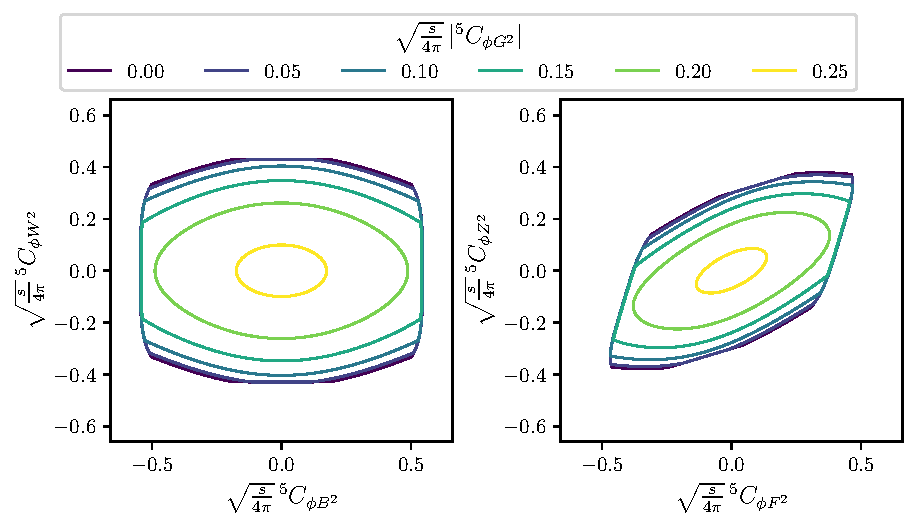
\includegraphics[scale = 0.92]{images/ALPs_d5_phiX2_combined_v2.pdf}
    \caption[Unitarity bounds on the dimension-five axion-like particle couplings to gauge bosons]{Plots of the boundaries of the parameter space allowed by the partial-wave unitarity bounds in Eq.~\eqref{eq:PWUB_d5_phiX2} in the $(\sqrt{s}\,\coef{5}{\phi B^2}{},\sqrt{s}\,\coef{5}{\phi W^2}{})$ plane (left panel) and in the $(\sqrt{s}\,\coef{5}{\phi F^2}{},\sqrt{s}\,\coef{5}{\phi Z^2}{})$ plane (right panel) for different values of $\sqrt{s}\,\abs*{\coef{5}{\phi G^2}{}}$. The Wilson coefficients $\coef{5}{\phi F^2}{}$ and $\coef{5}{\phi Z^2}{}$ are defined as $\coef{5}{\phi F^2}{} = c^2_{\rm W} \, \coef{5}{\phi B^2}{} + s^2_{\rm W}\,\coef{5}{\phi W^2}{}$ and $\coef{5}{\phi Z^2}{} = s^2_{\rm W} \, \coef{5}{\phi B^2}{} + c^2_{\rm W}\,\coef{5}{\phi W^2}{}$ (where $s_{\rm W}$ and $c_{\rm W}$ are the sine and cosine of the weak mixing angle) and mediate the interactions of the ALP with photons and $Z$ bosons, respectively: $\mathcal L \supset \coef{5}{\phi F^2}{} \, \phi \, F_{\mu\nu}\widetilde F^{\mu\nu} + \coef{5}{\phi Z^2}{} \, \phi \, Z_{\mu\nu}\widetilde Z^{\mu\nu}$.}
    \label{fig:d5phiX2}
\end{figure}


\subsubsection{$\phi \psi^2 H$ Class\label{par:phipsi2H}}

The individual bounds for this class of Wilson coefficients are
\begin{gather}
    s \sum_{p,r}\abs{\coef{5}{\phi \ell e H}{pr}}^2 \le 64\pi^2\,,
    \qquad
    s \sum_{p,r}\abs{\coef{5}{\phi qu H}{pr}}^2 \le \frac{64}{3}\pi^2\,,
    \qquad
    s \sum_{p,r}\abs{\coef{5}{\phi qd H}{pr}}^2 \le \frac{64}{3}\pi^2\,,
\end{gather}
while the combined bound is
\begin{equation}
    s \sum_{p,r}\left(\abs{\coef{5}{\phi \ell e H}{pr}}^2 + 3\abs{\coef{5}{\phi qu H}{pr}}^2+3\abs{\coef{5}{\phi qd H}{pr}}^2 \right) \le 64\pi^2\,.
\end{equation}
These are derived from the $J=0$ partial-wave coefficients of the amplitudes for $\phi H \to \psi_p \overline \psi_r$.

\subsubsection{$\phi^2 H^2 D^2$ Class\label{par:phi2H2D2}}

The bound for this Wilson coefficient is
\begin{equation}
    s \abs{\coef{6}{\phi ^2 H^2}{}} \le 8\pi\,,
\end{equation}
which is derived from the $J=0$ partial-wave coefficients of the amplitudes for $\phi \phi \to H\overline H$.

In Figure~\ref{fig:d56summary}, we summarize the marginalized partial-wave unitarity bounds on the Wilson coefficients associated with the dimension-five and -six ALP operators.

\begin{figure}[tb]
    \centering
    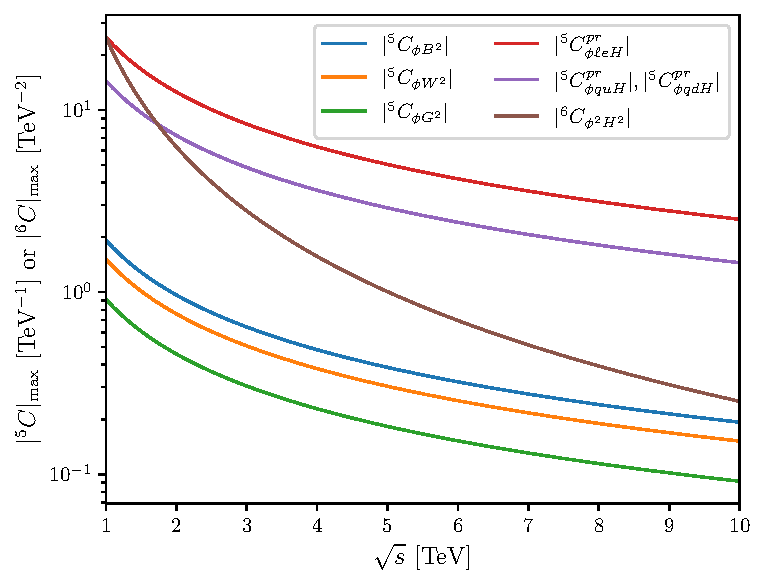
\includegraphics[scale = 0.92]{images/ALPs_d56_summary.pdf}
    \caption[Unitarity bounds on dimension-five and dimension-six axion-like particle operators]{Summary of the marginalized partial-wave unitarity bounds on the Wilson coefficients associated with the dimension-five and -six ALP operators.}
    \label{fig:d56summary}
\end{figure}

\subsection{Dimension-Seven Operators}

The dimension-seven ALP operators are reported in Table~\ref{tab:ALPdim7}.

\subsubsection{$\phi \psi^2 H D^2$ Class\label{par:phipsi2HD2}}

The individual bounds for this class of Wilson coefficients are
\begin{gather}
    s^3 \sum_{p,r}\abs{\coef{7}{\phi \ell e H}{(1)pr} + \coef{7}{\phi \ell e H}{(2)pr}}^2 \le 1024\pi^2\,, \label{eq:PWUB_d7_phipsi2HD2_1}
    \\
    s^{3/2} \abs{3\,\coef{7}{\phi \ell e H}{(1)pr} - \coef{7}{\phi \ell e H}{(2)pr}} \le 96\pi\,,
    \qquad
    s^{3/2} \abs{\coef{7}{\phi \ell e H}{(1)pr} - 3\, \coef{7}{\phi \ell e H}{(2)pr}} \le 96\pi\,,
    \\
    s^3 \sum_{p,r}\abs{\coef{7}{\phi qu H}{(1)pr} + \coef{7}{\phi qu H}{(2)pr}}^2 \le \frac{1024}{3}\pi^2\,,
    \\
    s^{3/2} \abs{3\,\coef{7}{\phi qu H}{(1)pr} - \coef{7}{\phi qu H}{(2)pr}} \le 96\pi\,,
    \qquad
    s^{3/2} \abs{\coef{7}{\phi qu H}{(1)pr} - 3\, \coef{7}{\phi qu H}{(2)pr}} \le 96\pi\,,
    \\
    s^3 \sum_{p,r}\abs{\coef{7}{\phi qd H}{(1)pr} + \coef{7}{\phi qd H}{(2)pr}}^2 \le \frac{1024}{3}\pi^2\,,
    \\
    s^{3/2} \abs{3\,\coef{7}{\phi qd H}{(1)pr} - \coef{7}{\phi qd H}{(2)pr}} \le 96\pi\,,
    \qquad
    s^{3/2} \abs{\coef{7}{\phi qd H}{(1)pr} - 3\, \coef{7}{\phi qd H}{(2)pr}} \le 96\pi\,, \label{eq:PWUB_d7_phipsi2HD2_2}
\end{gather}
while the combined bound is
\begin{equation}
    s^3
    \sum_{p,r}\left(
    \abs{\coef{7}{\phi \ell e H}{(1)pr} + \coef{7}{\phi \ell e H}{(2)pr}}^2
    + 3
    \abs{\coef{7}{\phi qu H}{(1)pr} + \coef{7}{\phi qu H}{(2)pr}}^2
    + 3
    \abs{\coef{7}{\phi qd H}{(1)pr} + \coef{7}{\phi qd H}{(2)pr}}^2
    \right)
     \le 1024\pi^2\,.
\end{equation}
These are derived from the $J=0$ partial-wave coefficients of the amplitudes for $\phi H \to \psi_p \overline \psi_r$ and the $J=1/2$ partial-wave coefficients of the amplitudes for $\phi \psi_p \to H \psi_r$.
The bounds are reported in Figure~\ref{fig:d7phipsi2H}.

\begin{figure}[tb]
    \centering
    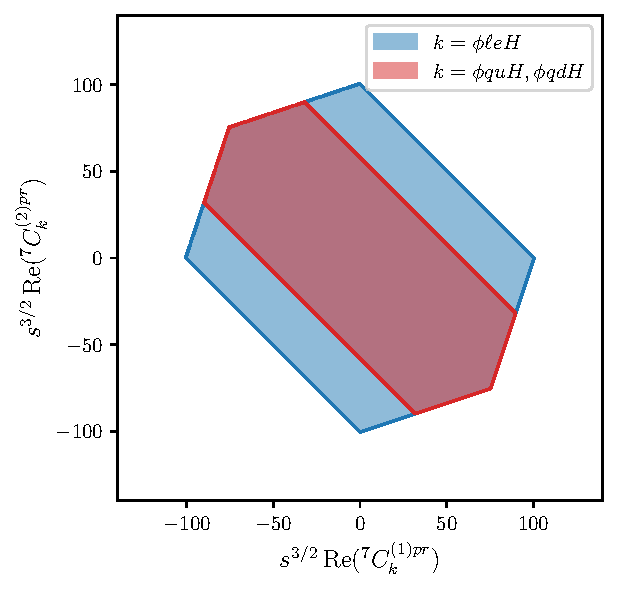
\includegraphics[scale = 0.92]{images/ALPs_d7_phipsi2H.pdf}
    \caption[Unitarity bounds on the dimension-seven axion-like particle operators of the class $\phi\psi^2HD^2$]{Parameter space allowed by partial-wave unitarity bounds in Eqs.~\eqref{eq:PWUB_d7_phipsi2HD2_1}--\eqref{eq:PWUB_d7_phipsi2HD2_2} associated with the dimension-seven operators $\op{7}{k}{(1)pr}$ and $\op{7}{k}{(2)pr}$, with $k=\phi \ell e H,\phi qu H,\phi qd H$ and $p,r=1,2,3$. The imaginary parts of the Wilson coefficients are set to zero.}
    \label{fig:d7phipsi2H}
\end{figure}

\subsubsection{$\phi \psi^2 X D$ Class\label{par:phipsi2XD}}

The bounds for the Wilson coefficients belonging to this class are
%
\begin{align}
    s^{3} \sum_{p,r} \abs{\coef{7}{\phi \ell^2 B}{(1)pr}+ i \,\coef{7}{\phi \ell^2 B}{(2)pr}}^2 &\le 288\pi^2\,,
     &
    s^{3} \sum_{p,r} \abs{\coef{7}{\phi e^2 B}{(1)pr}+ i \,\coef{7}{\phi e^2 B}{(2)pr}}^2 &\le 576\pi^2\,,    
    \\
    s^{3} \sum_{p,r} \abs{\coef{7}{\phi q^2 B}{(1)pr}+ i \,\coef{7}{\phi q^2 B}{(2)pr}}^2 &\le 96 \pi^2\,,
    &
    s^{3} \sum_{p,r} \abs{\coef{7}{\phi u^2 B}{(1)pr}+ i \,\coef{7}{\phi u^2 B}{(2)pr}}^2 &\le 192 \pi^2\,,
    \\
    s^{3} \sum_{p,r} \abs{\coef{7}{\phi d^2 B}{(1)pr}+ i \,\coef{7}{\phi d^2 B}{(2)pr}}^2 &\le 192 \pi^2\,,
    &
    s^{3} \sum_{p,r} \abs{\coef{7}{\phi \ell^2 W}{(1)pr}+ i \,\coef{7}{\phi \ell^2 W}{(2)pr}}^2 &\le 288\pi^2\,,
    \\
    s^{3} \sum_{p,r} \abs{\coef{7}{\phi q^2 W}{(1)pr}+ i \,\coef{7}{\phi q^2 W}{(2)pr}}^2 &\le 96 \pi^2\,,
    &
    s^{3} \sum_{p,r} \abs{\coef{7}{\phi q^2 G}{(1)pr}+ i \,\coef{7}{\phi q^2 G}{(2)pr}}^2 &\le 144 \pi^2\,, 
    \\
    s^{3} \sum_{p,r} \abs{\coef{7}{\phi u^2 G}{(1)pr}+ i \,\coef{7}{\phi u^2 G}{(2)pr}}^2 &\le 288 \pi^2\,,
    & 
    s^{3} \sum_{p,r} \abs{\coef{7}{\phi d^2 G}{(1)pr}+ i \,\coef{7}{\phi d^2 G}{(2)pr}}^2 &\le 288 \pi^2\,.
\end{align}
These are derived from the $J=1$ partial-wave coefficients of the amplitudes for $\phi X \to \psi_p \overline \psi_r$.

\subsubsection{$\phi X H^2 D^2$ Class\label{par:phiXH2D2}}

The bounds for the Wilson coefficients belonging to this class are
\begin{equation}
s^{3/2}\abs{\coef{7}{\phi B H^2}{(1)}+ i \,\coef{7}{\phi B H^2}{(2)}} \le 24\pi\,,
\qquad
s^{3/2}\abs{\coef{7}{\phi W H^2}{(1)}+ i \,\coef{7}{\phi W H^2}{(2)}} \le 24\pi\,.
\end{equation}
These are derived from the $J=1$ partial-wave coefficients of the amplitudes for $\phi X \to H \overline H$.


\subsubsection{$\phi H^4 D^2$ Class\label{par:phiH4D2}}
From the $J=0$ partial-wave coefficients of the amplitudes for $\phi H \to HH\overline H$ we obtain
\begin{equation}
    s^{3/2} \abs{\coef{7}{\phi H^4}{}} \le 16\sqrt{6}\pi^2\,.
\end{equation}

\subsubsection{$\phi \psi^2 H^2 D$ Class\label{par:phipsi2H2D}}
The individual bounds for the Wilson coefficients belonging to this class are
\begin{gather}
    s^3 \sum_{p,r}\abs{\coef{7}{\phi \ell^2 H^2}{(1)pr}}^2 \le (32\sqrt{6}\pi^2)^2 \,,
    \qquad 
    s^3 \sum_{p,r}\abs{\coef{7}{\phi \ell^2 H^2}{(2)pr}}^2 \le (32\sqrt{6}\pi^2)^2 \,,
    \\
    s^3 \sum_{p,r}\abs{\coef{7}{\phi q^2 H^2}{(1)pr}}^2 \le (32\sqrt{2}\pi^2)^2 \,,
    \qquad 
    s^3 \sum_{p,r}\abs{\coef{7}{\phi q^2 H^2}{(2)pr}}^2 \le (32\sqrt{2}\pi^2)^2  \,,
    \\
    s^3 \sum_{p,r}\abs{\coef{7}{\phi e^2 H^2}{pr}}^2 \le (64\sqrt{3}\pi^2)^2 \,,
    \;\,\, 
    s^3 \sum_{p,r}\abs{\coef{7}{\phi u^2 H^2}{pr}}^2 \le (64\pi^2)^2  \,,
    \;\,\,
    s^3 \sum_{p,r}\abs{\coef{7}{\phi d^2 H^2}{pr}}^2 \le (64\pi^2)^2  \,.
\end{gather}
They are derived from the $J=0$ partial-wave coefficients of the amplitudes for $H \overline H \to \phi \psi_p \overline \psi_{r}$.
%
The combined bounds are
\begin{gather}
s^3 \sum_{p,r}\left(\abs{\coef{7}{\phi \ell^2 H^2}{(2)pr}}^2+3\abs{\coef{7}{\phi q^2 H^2}{(2)pr}}^2\right) \le (32\sqrt{6}\pi^2)^2\,,
\\
    s^3 \sum_{p,r}\left(\abs{\coef{7}{\phi e^2 H^2}{pr}}^2 + 3\abs{\coef{7}{\phi u^2 H^2}{pr}}^2+3\abs{\coef{7}{\phi d^2 H^2}{pr}}^2+2\abs{\coef{7}{\phi \ell^2 H^2}{(1)pr}}^2+6\abs{\coef{7}{\phi q^2 H^2}{(1)pr}}^2\right) \le (64\sqrt{3}\pi^2)^2\,.
\end{gather}

In Figure~\ref{fig:d7summary}, we summarize the marginalized partial-wave unitarity bounds on the Wilson coefficients associated with the dimension-seven ALP operators.

\begin{figure}[tb]
    \centering
    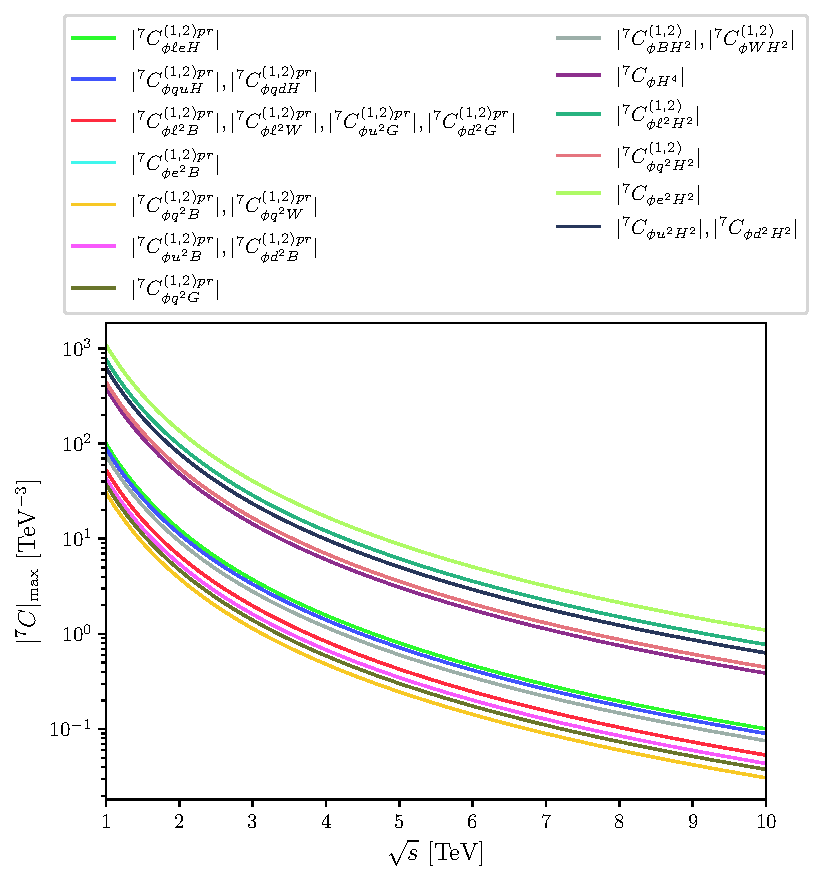
\includegraphics[scale = 0.92]{images/ALPs_d7_summary.pdf}
    \caption[Unitarity bounds on dimension-seven axion-like particle operators]{Summary of the marginalized partial-wave unitarity bounds on the Wilson coefficients associated with the dimension-seven ALP operators.}
    \label{fig:d7summary}
\end{figure}

\subsection{Dimension-Eight Operators}

The dimension-eight ALP operators that conserve lepton and baryon numbers are reported in Table~\ref{tab:ALPdim8}.

\subsubsection{$\phi^4 D^4$ Class\label{par:phi4D4}}
The strongest partial-wave unitarity bound for this Wilson coefficient is
\begin{equation}
    s^2 \abs{\coef{8}{\phi^4}{}} \le \frac{24}{5}\pi
\end{equation}
and is derived from the $J=0$ partial-wave coefficient of the amplitude for $\phi \phi \to \phi \phi$.

\subsubsection{$\phi^2 H^4 D^2$ Class\label{par:phi2H4D2}}
The strongest partial-wave unitarity bound for this Wilson coefficient is
\begin{equation}
    s^2 \abs{\coef{8}{\phi^2 H^4}{}} \le 128\sqrt{2}\pi^3
\end{equation}
and is derived from the $J=0$ partial-wave coefficients of the amplitudes for $\phi \phi \to H\overline HH\overline H$.

\subsubsection{$\phi^2 H^2 D^4$ Class\label{par:phi2H2D4}}
The partial-wave unitarity bounds for this class of Wilson coefficients are
\begin{equation}
    \label{eq:d8-uni_phi2H2}
    s^2 \abs{3\, \coef{8}{\phi^2 H^2}{(1)}+\coef{8}{\phi^2 H^2}{(2)}} \le 48 \pi\,, 
    \qquad 
    s^2  \abs{\coef{8}{\phi^2 H^2}{(1)}+2\, \coef{8}{\phi^2 H^2}{(2)}} \le 48 \pi\,,
\end{equation}
which are derived from the $J=0$ partial-wave coefficients of the amplitudes for $\phi \phi \to H\overline H$ and $\phi H \to \phi H$.
They are shown in Figure~\ref{fig:d8phi2H2}.

\subsubsection{$\phi^2 X^2 D^2$ Class\label{par:phi2X2D2}}
The individual bounds for this class of Wilson coefficients are
\begin{gather}\label{eq:PWUB_d8_phi2X2_1}
s^2 \sqrt{\left(\coef{8}{\phi^2 B^2}{(1)}+4\,\coef{8}{\phi^2 B^2}{(2)}\right)^2+\left(4\,\coef{8}{\phi^2 B^2}{(3)}\right)^2} \le 16 \sqrt{2}\pi\,, \\
s^2 \left[8\abs{\coef{8}{\phi^2 B^2}{(1)}}+3\sqrt{\left(\coef{8}{\phi^2 B^2}{(1)}+4\,\coef{8}{\phi^2 B^2}{(2)}\right)^2+\left(4\,\coef{8}{\phi^2 B^2}{(3)}\right)^2}\right]\le 192 \pi\,,
\\
s^2 \sqrt{\left(\coef{8}{\phi^2 W^2}{(1)}+4\,\coef{8}{\phi^2 W^2}{(2)}\right)^2+\left(4\,\coef{8}{\phi^2 W^2}{(3)}\right)^2} \le 16 \sqrt{\frac{2}{3}}\pi\,, 
\\
s^2 \left[8\abs{\coef{8}{\phi^2 W^2}{(1)}}+3\sqrt{\left(\coef{8}{\phi^2 W^2}{(1)}+4\,\coef{8}{\phi^2 W^2}{(2)}\right)^2+\left(4\,\coef{8}{\phi^2 W^2}{(3)}\right)^2}\right]\le 192 \pi\,,
\\
s^2 \sqrt{\left(\coef{8}{\phi^2 G^2}{(1)}+4\,\coef{8}{\phi^2 G^2}{(2)}\right)^2+\left(4\,\coef{8}{\phi^2 G^2}{(3)}\right)^2} \le 8\pi\,,
\\
s^2 \left[8\abs{\coef{8}{\phi^2 G^2}{(1)}}+3\sqrt{\left(\coef{8}{\phi^2 G^2}{(1)}+4\,\coef{8}{\phi^2 G^2}{(2)}\right)^2+\left(4\,\coef{8}{\phi^2 G^2}{(3)}\right)^2}\right]\le 192 \pi\,,
\label{eq:PWUB_d8_phi2X2_2}
\end{gather}
while the combined one is
\begin{align}
    s^4\bigg[&\left(\coef{8}{\phi^2 B^2}{(1)}+4\,\coef{8}{\phi^2 B^2}{(2)}\right)^2+\left(4\,\coef{8}{\phi^2 B^2}{(3)}\right)^2 + 3 \left(\coef{8}{\phi^2 W^2}{(1)}+4\,\coef{8}{\phi^2 W^2}{(2)}\right)^2+3\left(4\,\coef{8}{\phi^2 W^2}{(3)}\right)^2\nonumber \\
    &+ 8\left(\coef{8}{\phi^2 G^2}{(1)}+4\,\coef{8}{\phi^2 G^2}{(2)}\right)^2+8\left(4\,\coef{8}{\phi^2 G^2}{(3)}\right)^2\bigg]\le (16\sqrt{2}\pi)^2\,.
\end{align}
These bounds are derived from the $J=0$ partial-wave coefficients of the amplitudes for $\phi \phi \to XX$ and the $J=1$ partial-wave coefficients of the amplitudes for $\phi X \to \phi X$.
They are shown in Figure~\ref{fig:d8phi2B2}.

\subsubsection{$\phi^2 \psi^2 D^3$ Class\label{par:phi2psi2D3}}

The strongest individual bounds are
\begin{equation}
    s^2 \abs{\coef{8}{\phi^2 \psi^2}{pr}} \le \frac{96}{5}\pi 
    \qquad
    \text{with~}
    \psi = \ell,e,q,u,d
\end{equation}
and are derived from the $J=1/2$ partial-wave coefficients of the amplitudes for $\phi \psi_p \to \phi \psi_r$.
%
The collective bound is
\begin{equation}
    s^4 \sum_{p,r}\bigg(
    \abs{\coef{8}{\phi^2 e^2}{pr}}^2 
    +2\abs{\coef{8}{\phi^2 \ell^2}{pr}}^2
    + 3 \abs{\coef{8}{\phi^2 u^2}{pr}}^2 
    + 3 \abs{\coef{8}{\phi^2 d^2}{pr}}^2
    + 6 \abs{\coef{8}{\phi^2 q^2}{pr}}^2 
    \bigg) \le (160\sqrt{3}\pi)^2
\end{equation}
and is derived from the $J=2$ partial-wave coefficients of the amplitudes for $\phi \phi \to \psi_p \overline \psi_r$.

\subsubsection{$\phi^2 \psi^2 H D^2$ Class\label{par:phi2psi2HD2}}
The individual bounds for this class of Wilson coefficients are
\begin{gather}
    s^4 \sum_{p,r}\abs{\coef{8}{\phi^2 \ell e H}{pr}}^2 \le (32\sqrt{3}\pi^2)^2\,,\\
    s^4 \sum_{p,r}\abs{\coef{8}{\phi^2 qu H}{pr}}^2 \le (32\pi^2)^2\,,
    \qquad 
    s^4 \sum_{p,r}\abs{\coef{8}{\phi^2 qd H}{pr}}^2 \le (32\pi^2)^2\,.
\end{gather}
%
The combined one is
\begin{equation}
    s^4 \sum_{p,r} \left(\abs{\coef{8}{\phi^2 \ell e H}{pr}}^2 + 3 \abs{\coef{8}{\phi^2 qu H}{pr}}^2 + 3 \abs{\coef{8}{\phi^2 qd H}{pr}}^2\right) \le (32\sqrt{3}\pi^2)^2\,.
\end{equation}
%
These are derived from the $J=0$ partial-wave coefficients of the amplitudes for $\phi \phi \to \psi_p \overline \psi_r H$.

In Figure~\ref{fig:d8summary}, we summarize the marginalized partial-wave unitarity bounds on the Wilson coefficients associated with the dimension-eight ALP operators.

\begin{figure}[tb]
    \centering
    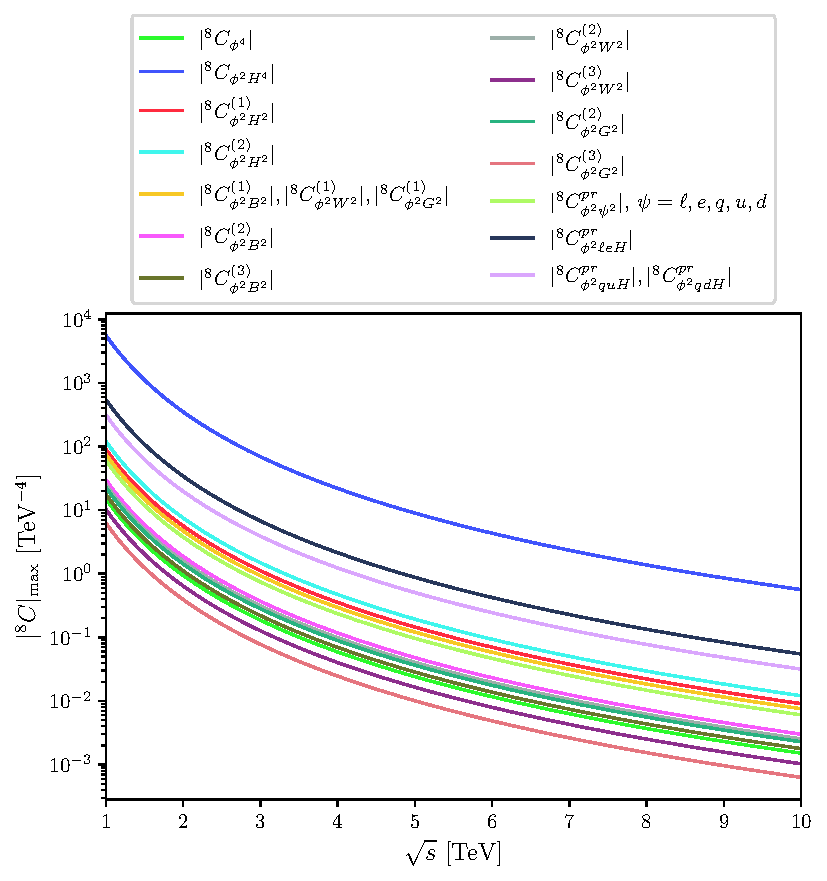
\includegraphics[scale = 0.92]{images/ALPs_d8_summary.pdf}
    \caption[Unitarity bounds on dimension-eight axion-like particle operators]{Summary of the marginalized partial-wave unitarity bounds on the Wilson coefficients associated with the dimension-eight ALP operators.}
    \label{fig:d8summary}
\end{figure}


\subsection{Weak-Violating Axion-Like Particle Interactions with Leptons}
%
The EFT assumed so far was invariant under the electroweak gauge group. If we give up this assumption, ALP-lepton interactions are described by the dimension-five 
Lagrangian~\cite{Altmannshofer:2022ckw}:
%
\begin{equation}
\mathcal{L} = \partial_\mu\phi\, \frac{\overline g_{ll }}{2m_l }\, \overline l  \gamma^\mu l  + \partial_\mu\phi\, \frac{g_{ll}}{2m_l}\, \overline l  \gamma^\mu \gamma_5 l  + \partial_\mu\phi\, \frac{g_{\nu _l }}{2m_l }\, \overline \nu_l \gamma^\mu P_L \nu_l \,,\qquad l = e,\, \mu,\, \tau,
\end{equation} 
%
where the $SU(2)_L$ invariance is recovered for $g_{\nu_l} = \overline g_{ll} - g_{ll}$. The implications of the above interactions are better understood by integrating by parts the Lagrangian~\cite{Altmannshofer:2022ckw}:
%
\begin{align}
-\mathcal{L} &= g_{ll} (\overline l i\gamma_5 l)\, \phi
+ \frac{ e ^2 }{ 16 \pi ^2 m _l } \bigg[ \frac{ \overline{g} _{ll} - 
g _{ll} + g _{\nu_l} }{ 4 s _{\rm W} ^2} W ^+ _{\mu\nu} \widetilde W ^{ {-}\mu \nu } \notag  + \frac{\overline{g} _{ll} - g _{ ll} ( 1 - 4  s _{\rm W} ^2 ) }{ 2 c _{\rm W} s _{\rm W} } F _{\mu\nu} \widetilde{Z} ^{\mu\nu}
\\
&\quad - g _{ll}  F _{\mu\nu} \widetilde{F} ^{\mu\nu} + \notag \frac{ \overline{g} _{ ll} ( 1 - 4 s _{\rm W} ^2 ) - g _{ll} ( 1 - 4 s _{\rm W} ^2 + 8 s _{\rm W} ^4 )  + g _{\nu _l } }{ 8 s _{\rm W} ^2 c _{\rm W} ^2 } Z _{\mu\nu} \widetilde{Z} ^{\mu\nu} \bigg] \,\phi \notag
\\
&\quad + \frac{ig}{2\sqrt{2} m _l }(g_{ll} - \overline g_{ll} + g_{\nu _l }) (\overline l \gamma^\mu P _L \nu_l) W_\mu^- \,\phi + \text{H.c.}\,, 
\label{eq:weak_violating}
\end{align}
%
where $s_{\rm W}$ ($c_{\rm W}$) is the sine (cosine) of the weak mixing angle.
All terms in Eq.~\eqref{eq:weak_violating} are generated 
in the $SU(2)_L$ symmetric limit, except for the last term, which is a genuine electroweak-violating interaction.
As shown in Ref.~\cite{Altmannshofer:2022ckw}, this term generates
an $ ({\rm energy} / m_l )$ enhancement in various processes such as charged meson decays and $W$ boson decays.

The most stringent unitarity bound for the weak-violating combination of coefficients $g_{ll}-\overline g_{ll} + g_{\nu_l}$ is
%
\begin{equation}\label{eq:WV_bounds}
    \frac{s}{m_W m_l}\, g\, \abs{g_{ll}-\overline g_{ll} + g_{\nu_l}} \le 32\sqrt{2}\pi\,,
\end{equation}
%
which is derived from the $J=1/2$ partial-wave coefficient of the amplitude for $\phi l \to W \nu_l$.
In particular, we have the following bounds
%
%
\begin{equation}
    \abs{g_{ll}-\overline g_{ll} + g_{\nu_l}} \lesssim 10^{-5} \left(\frac{m_l}{m_e}\right)
    \left(\frac{\text{TeV}}{\sqrt{s}}\right)^2\,,
\end{equation}
%
which are reported in Figure~\ref{fig:WV}.

\begin{figure}[tb]
    \centering
    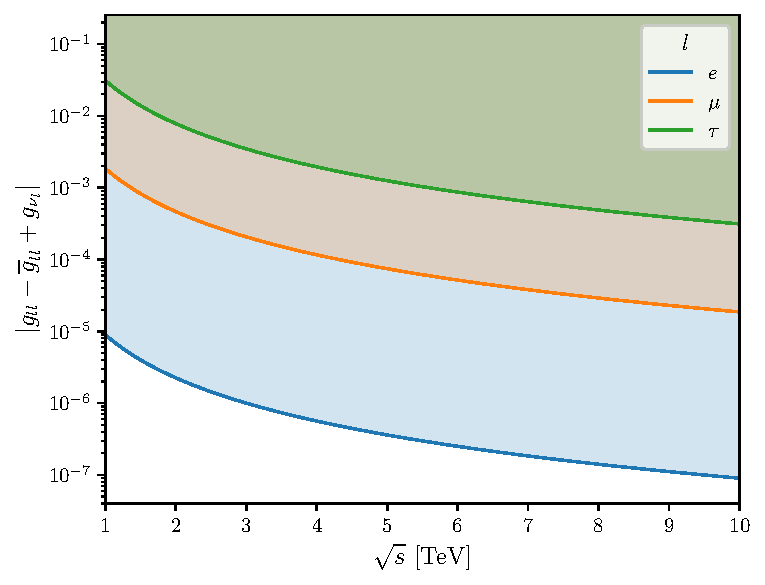
\includegraphics[scale = 0.92]{images/ALPs_WV.pdf}
    \caption[Unitarity bounds on weak-violating axion-like particle couplings to leptons]{Excluded values of the weak-violating combinations $\abs{g_{ll}-\overline{g}_{ll}+g_{\nu_l}}$ as functions of the center-of-mass energy $\sqrt{s}$ by imposing the partial-wave unitarity bounds of Eq.~\eqref{eq:WV_bounds}.}
    \label{fig:WV}
\end{figure}


\section{Positivity Bounds}
\label{sec:positivity}

Positivity bounds, stemming from the requirement that an EFT is the low-energy limit of a unitary, local, and causal quantum field theory~\cite{Adams:2006sv},
provide another set of conditions to infer the viable parameter space of consistent EFTs. 
Hereafter, we evaluate the complete set 
of positivity bounds for ALP EFTs, 
associated with dimension-eight operators,
discussing their complementarity and interplay with partial-wave unitarity constraints~\cite{Bresciani:2025toe}.

Positivity bounds are derived from elastic $2 \to 2$ scattering processes whose amplitudes grow with even powers $n$ of $s$, with $n \ge 2$. 
By considering the scattering of a superposition of states $\ket{u} = \sum_i u_i \ket{i}$ and $\ket{v} = \sum_j v_j \ket{j}$
\begin{equation}
    \mathcal A (s,t) = \mathcal A(u,v \to u,v) = \sum_{i,j,k,l} u_i^* v_j^* u_k v_l \, \mathcal A(i,j\to k,l) \,,
\end{equation}
we can set in the forward limit \cite{Adams:2006sv,Bellazzini:2016xrt}
\begin{equation}
    \left.\dv[2]{}{s} \mathcal A(s,0)\right|_{s=0} \ge 0\,.
\end{equation}

For example, with regard to the operators $\op{8}{\phi^2 H^2}{(1)}$ and $\op{8}{\phi^2 H^2}{(2)}$, if we take 
\begin{equation}
    \ket{u} = \ket{\phi} + x \ket{\pi_a} \,, \qquad \ket{v} = \ket{\phi} + \ket{\pi_a}\,,
\end{equation}
where $\pi_a$ is any of the real components of the Higgs doublet
\begin{equation}
    H =\frac{1}{\sqrt{2}} \begin{pmatrix}
        \pi_1 + i\, \pi_3 \\ \pi_2 + i\, \pi_4 
    \end{pmatrix}\,,
\end{equation}
the amplitude is
\begin{align}
    \mathcal A (s,\theta) &= \mathcal A (u,v \to u,v) \nonumber\\&
    = \frac{s^2}{32}\bigg[
    \coef{8}{\phi^2 H^2}{(1)}\,(6 + 44x + 6x^{2})
  + \coef{8}{\phi^2 H^2}{(2)}\,(11+34x+11x^2)
  \nonumber  \\&\quad - 4 \left(2\,\coef{8}{\phi^2 H^2}{(1)} - \coef{8}{\phi^2 H^2}{(2)}\right)(1 - x)^{2}\cos\theta \nonumber  \\&\quad
  + \left(2\,\coef{8}{\phi^2 H^2}{(1)}\,(1 + x)^{2} + \coef{8}{\phi^2 H^2}{(2)}\,(1+6x+x^2)\right)\cos(2\theta)
\bigg]
\end{align}
and in the forward limit reduces to
\begin{equation}
    \mathcal A (s,0) = \frac{s^2}{2}\left[4\, \coef{8}{\phi^2 H^2}{(1)}\,x +  \coef{8}{\phi^2 H^2}{(2)}\, (1+x)^2\right]\,,
\end{equation}
leading to the bound in Eq.~\eqref{eq:d8-pos_phi2H2} by imposing $4\, \coef{8}{\phi^2 H^2}{(1)}\,x +  \coef{8}{\phi^2 H^2}{(2)} \,(1+x)^2 \ge 0$ for every $x \in \mathbb{R}$.

Another example is provided by the operators $\op{8}{\phi^2 B^2}{(1)}$, $\op{8}{\phi^2 B^2}{(2)}$, and $\op{8}{\phi^2 B^2}{(3)}$.
By parameterizing $\ket{u}$ and $\ket{v}$ as
\begin{equation}
    \ket{u} = \ket{\phi}+x_-\ket{B^-}+x_+\ket{B^+}\,,
    \qquad 
    \ket{v} = \ket{\phi}+y_-\ket{B^-}+y_+\ket{B^+}\,,
\end{equation}
and by using the amplitudes reported in Eqs.~\eqref{eq:ampl_d8_phi2B2(1)} and \eqref{eq:ampl_d8_phi2B2(2)},
the second derivative of $\mathcal A(s,\theta) = \mathcal A(u,v \to u,v)$ with respect to $s$ in the forward limit can be written as
\begin{equation}
    \left.\dv[2]{}{s}\mathcal A(s,0)\right|_{s=0} = \mathbf V\,\mathbf A\,\mathbf V^{T}\,,
\end{equation}
with
\begin{align}
    \mathbf V &=
    \begin{pmatrix}
        \Re x_- & \Im x_- & \Re x_+ & \Im x_+ & \Re y_- & \Im y_- & \Re y_+ & \Im y_+
    \end{pmatrix}\,,
    \\
    \mathbf A &=
    \begin{pmatrix}
-2\,\coef{8}{\phi^2 B^2}{(1)}\,\mathbb{I}_{4} & \mathbf B \\
\mathbf B & -2\,\coef{8}{\phi^2 B^2}{(1)}\,\mathbb{I}_{4}
\end{pmatrix}\,,
\end{align}
and
\begin{equation}
    \mathbf B=
    \begin{pmatrix}
\coef{8}{\phi^2 B^2}{(1)} + 4\,\coef{8}{\phi^2 B^2}{(2)} & -4\,\coef{8}{\phi^2 B^2}{(3)} & \coef{8}{\phi^2 B^2}{(1)} + 4\,\coef{8}{\phi^2 B^2}{(2)} & 4\,\coef{8}{\phi^2 B^2}{(3)} \\
-4\,\coef{8}{\phi^2 B^2}{(3)} & -\coef{8}{\phi^2 B^2}{(1)} - 4\,\coef{8}{\phi^2 B^2}{(2)} & -4\,\coef{8}{\phi^2 B^2}{(3)} & \coef{8}{\phi^2 B^2}{(1)} + 4\,\coef{8}{\phi^2 B^2}{(2)} \\
\coef{8}{\phi^2 B^2}{(1)} + 4\,\coef{8}{\phi^2 B^2}{(2)} & -4\,\coef{8}{\phi^2 B^2}{(3)} & \coef{8}{\phi^2 B^2}{(1)} + 4\,\coef{8}{\phi^2 B^2}{(2)} & 4\,\coef{8}{\phi^2 B^2}{(3)} \\
4\,\coef{8}{\phi^2 B^2}{(3)} & \coef{8}{\phi^2 B^2}{(1)} + 4\,\coef{8}{\phi^2 B^2}{(2)} & 4\,\coef{8}{\phi^2 B^2}{(3)} & -\coef{8}{\phi^2 B^2}{(1)} - 4\,\coef{8}{\phi^2 B^2}{(2)}
\end{pmatrix}\,.
\end{equation}
Finally, by imposing $\mathbf A \succeq 0$, one obtains the constraint in Eq.~\eqref{eq:d8-pos_phi2X2}.

In the following, we present the complete set of positivity bounds associated with the dimension-eight ALP operators listed in Table~\ref{tab:ALPdim8}, and, in Appendix~\ref{app:UVext}, we test them against a specific ultraviolet extension.

\subsubsection{$\phi^4 D^4$ Class}

The positivity bound related to this operator reads~\cite{Ananthanarayan:1994hf,Adams:2006sv}
%
\begin{equation}
    \coef{8}{\phi^4}{} \ge 0\,.
\end{equation}

\subsubsection{$\phi^2 H^2 D^4$ Class}

The positivity bound for this class of Wilson coefficients, 
obtained by considering all possible superpositions of scattering states, is shown in Figure~\ref{fig:d8phi2H2} and reads
\begin{equation}
    \coef{8}{\phi^2 H^2}{(2)}-\abs{2\,\coef{8}{\phi^2 H^2}{(1)}+\coef{8}{\phi^2 H^2}{(2)}} \ge 0\,,
    \label{eq:d8-pos_phi2H2}
\end{equation}
whereas the bound obtained without including such superpositions is
\begin{equation}
    \coef{8}{\phi^2 H^2}{(2)} \ge 0\,.
\end{equation}
They are consistent with those of~\cite{Kim:2023pwf}.

\begin{figure}[tb]
    \centering
    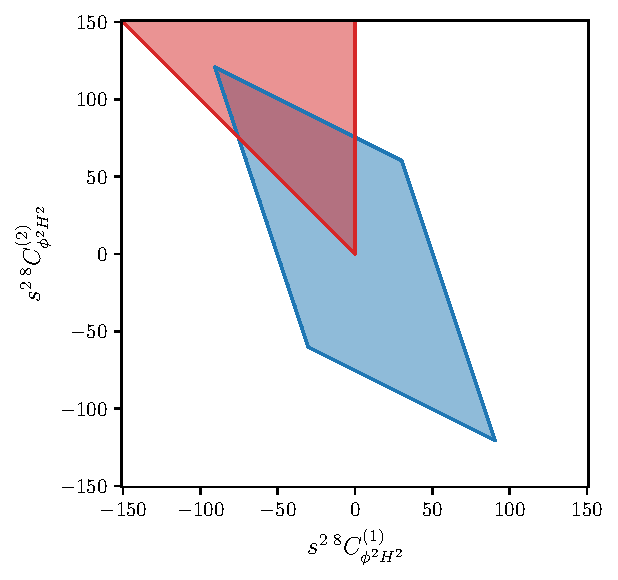
\includegraphics[scale = 0.92]{images/ALPs_d8_phi2H2.pdf}
    \caption[Unitarity and positivity bounds on the dimension-eight class $\phi^2H^2D^4$]{Parameter space allowed by partial-wave unitarity bounds (Eq.~\eqref{eq:d8-uni_phi2H2}, blue) and positivity bounds (Eq.~\eqref{eq:d8-pos_phi2H2}, red) associated with the operators $\op{8}{\phi^2 H^2}{(1)}$ and $\op{8}{\phi^2 H^2}{(2)}$. The intersection area constitutes $1/4$ of the area of the blue region.}
    \label{fig:d8phi2H2}
\end{figure}

\subsubsection{$\phi^2 X^2 D^2$ Class}

The positivity bounds for this class of Wilson coefficients, obtained by considering all possible superpositions of scattering states, are
\begin{equation}
\label{eq:d8-pos_phi2X2}
    \coef{8}{\phi^2 X^2}{(1)} + \sqrt{\left(\coef{8}{\phi^2 X^2}{(1)}+4\,\coef{8}{\phi^2 X^2}{(2)}\right)^2+\left(4\,\coef{8}{\phi^2 X^2}{(3)}\right)^2} \le 0
\end{equation}
for every $X=B,W,G$, and are shown in Figure~\ref{fig:d8phi2B2}, whereas the bounds obtained without including such superpositions are
\begin{equation}
    \coef{8}{\phi^2 X^2}{(1)} \le 0\,.
\end{equation}

\begin{figure}[tb]
    \centering
    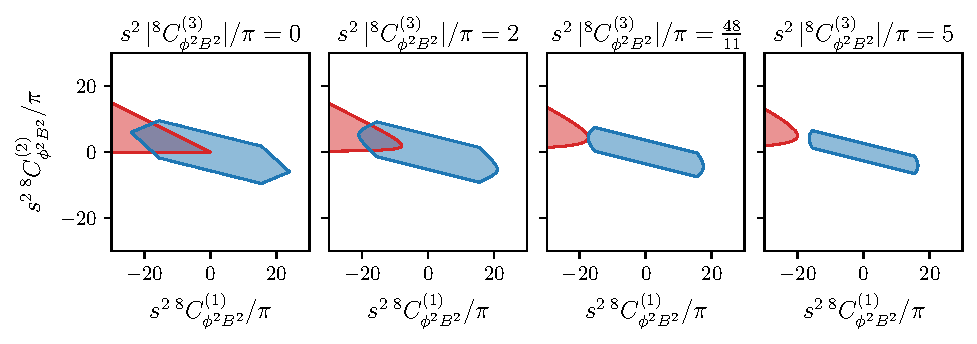
\includegraphics[width=\linewidth]{images/ALPs_d8_phi2B2.pdf}
    \\
    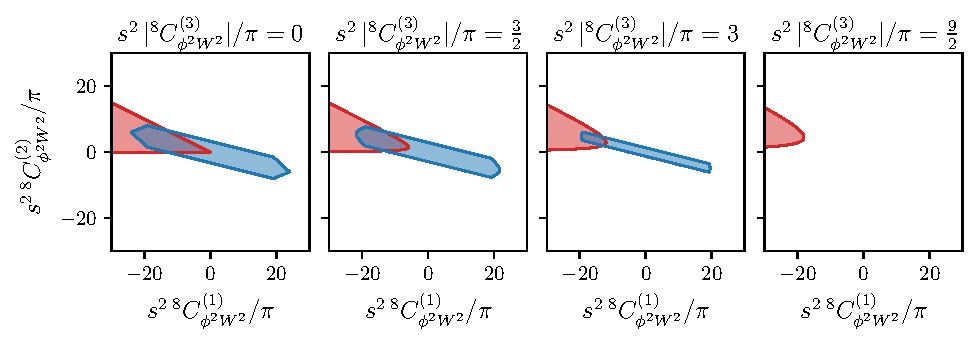
\includegraphics[width=\linewidth]{images/ALPs_d8_phi2W2.pdf}
    \\
    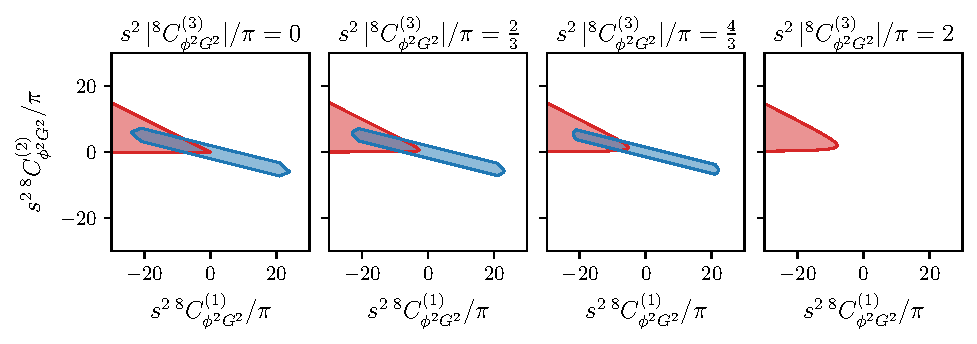
\includegraphics[width=\linewidth]{images/ALPs_d8_phi2G2.pdf}
    \caption[Unitarity and positivity bounds on the dimension-eight class $\phi^2X^2D^2$]{Parameter space allowed by the partial-wave unitarity bounds 
    (Eqs.~\eqref{eq:PWUB_d8_phi2X2_1}--\eqref{eq:PWUB_d8_phi2X2_2}, blue)
    and the positivity constraints 
    (Eq.~\eqref{eq:d8-pos_phi2X2}, red)
    concerning the Wilson coefficients belonging to the class $\phi^2 X^2 D^2$ in the $(s^2\,\coef{8}{\phi^2 X^2}{(1)},s^2\,\coef{8}{\phi^2 X^2}{(2)})$ plane and computed for different values of $s^2\,\abs*{\coef{8}{\phi^2 X^2}{(3)}}$.}
    \label{fig:d8phi2B2}
\end{figure}

To highlight the impact of positivity bounds, we compare the volume of the parameter space allowed by unitarity (see Eqs.~\eqref{eq:PWUB_d8_phi2X2_1}--\eqref{eq:PWUB_d8_phi2X2_2}), $\text{Vol}(\mathscr U)$, with the one obtained after imposing the positivity constraints in Eq.~\eqref{eq:d8-pos_phi2X2}, $\text{Vol}(\mathscr U \cap \mathscr P)$.
In particular, for fixed values of the center-of-mass energy, we find
\begin{equation}
    \frac{\text{Vol}(\mathscr U \cap \mathscr P)}{\text{Vol}(\mathscr U)} = 
    \begin{dcases}
        \frac{36(6+\sqrt{2})}{2057}\approx 0.13 & \text{if~}d(G)=1,\\
        \frac{18\sqrt{d(G)}-11\sqrt{2}}{36\sqrt{d(G)}-6\sqrt{2}} &\text{if~}d(G)\ge 2,
    \end{dcases}
\end{equation}
depending on the dimensionality $d(G)$ of the associated gauge group $G$.

These bounds also apply if we substitute the ALP field with a Higgs doublet.
If one performs this substitution, one finds the dimension-eight SMEFT operators
\begin{align}
    Q^{(1)}_{X^2 H^2 D^2} &= (D^\mu H^\dagger D^\nu H)X^{\mathscr A}_{ \mu\rho}X_\nu^{\mathscr A\rho}\,,
    \\
    Q^{(2)}_{X^2 H^2 D^2} &= (D^\mu H^\dagger D_\mu H)X^{\mathscr A}_{ \nu\rho}X^{\mathscr A \nu \rho}\,,
    \\
    Q^{(3)}_{X^2 H^2 D^2} &= (D^\mu H^\dagger D_\mu H)X^{\mathscr A}_{ \nu\rho}\widetilde X^{\mathscr A \nu \rho}\,,
\end{align}
with $X_{\mu\nu}^{\mathscr A} = B_{\mu\nu},W_{\mu\nu}^I,G_{\mu\nu}^A$, of the basis in \cite{Murphy:2020rsh}.
It follows that the associated Wilson coefficients satisfy the constraints
\begin{equation}
    C_{X^2 H^2 D^2}^{(1)} + \sqrt{\left(C_{X^2 H^2 D^2}^{(1)}+4\,C_{X^2 H^2 D^2}^{(2)}\right)^2+\left(4\,C_{X^2 H^2 D^2}^{(3)}\right)^2} \le 0
\end{equation}
for every $X=B,W,G$,
which represent a generalization of the results presented in \cite{Chala:2023xjy,Remmen:2019cyz} that accounts for a non-vanishing CP-odd $C_{X^2 H^2 D^2}^{(3)}$.

\subsubsection{$\phi^2 \psi^2 D^3$ Class}
The positivity bounds for this class of Wilson coefficients, obtained by considering all possible superpositions of scattering states, are
\begin{equation}
    \coef{8}{\phi^2\psi^2}{} \succeq 0\,,
\end{equation}
or, equivalently,
\begin{align}
\label{eq:pos_d8_phi2psi2_1}
    0\le \Tr (\coef{8}{\phi^2 \psi^2}{}) &= \coef{8}{\phi^2 \psi^2}{11}+\coef{8}{\phi^2 \psi^2}{22}+\coef{8}{\phi^2 \psi^2}{33}\,,
    \\
    0 \le \frac{1}{2}\left[\left(\Tr (\coef{8}{\phi^2 \psi^2}{}) \right)^2 - \Tr (\coef{8}{\phi^2 \psi^2}{2})\right] &= \coef{8}{\phi^2 \psi^2}{11}\,\coef{8}{\phi^2 \psi^2}{22}+\coef{8}{\phi^2 \psi^2}{11}\,\coef{8}{\phi^2 \psi^2}{33}+\coef{8}{\phi^2 \psi^2}{22}\,\coef{8}{\phi^2 \psi^2}{33}\nonumber \\&\quad -\abs{\coef{8}{\phi^2 \psi^2}{12}}^2-\abs{\coef{8}{\phi^2 \psi^2}{13}}^2-\abs{\coef{8}{\phi^2 \psi^2}{23}}^2\,, \label{eq:pos_d8_phi2psi2_2} \\
    0\le \det (\coef{8}{\phi^2 \psi^2}{}) &= \coef{8}{\phi^2 \psi^2}{11}\,\coef{8}{\phi^2 \psi^2}{22}\,\coef{8}{\phi^2 \psi^2}{33}+\coef{8}{\phi^2 \psi^2}{12}\,\coef{8}{\phi^2 \psi^2}{23}\,\coef{8}{\phi^2 \psi^2}{31}\nonumber \\
    &\quad+
    \coef{8}{\phi^2 \psi^2}{13}\,\coef{8}{\phi^2 \psi^2}{32}\,\coef{8}{\phi^2 \psi^2}{21}
    -\coef{8}{\phi^2 \psi^2}{11}\abs{\coef{8}{\phi^2 \psi^2}{23}}^2\nonumber \\
    &\quad-\coef{8}{\phi^2 \psi^2}{22}\abs{\coef{8}{\phi^2 \psi^2}{13}}^2-\coef{8}{\phi^2 \psi^2}{33}\abs{\coef{8}{\phi^2 \psi^2}{12}}^2\,, \label{eq:pos_d8_phi2psi2_3}
\end{align}
for every $\psi = \ell,e,q,u,d$.
This means that:
\begin{itemize}
    \item Every diagonal entry of $\coef{8}{\phi^2 \psi^2}{}$ must be positive;
    \item The modulus of the off-diagonal entries of $\coef{8}{\phi^2 \psi^2}{}$ is bounded from above by combinations of its diagonal entries.
\end{itemize}
Instead, if one did not consider all possible superpositions of scattering states, the resulting bound would just involve the diagonal entries:
\begin{equation}
    \coef{8}{\phi^2 \psi^2}{pp} \ge 0\,.
\end{equation}

Also in this case, by substituting the ALP field with a Higgs doublet, one recovers the dimension-eight SMEFT operators 
\begin{align}
    Q_{\psi^2 H^2 D^3}^{(1)pr} &= i(\overline \psi_p \gamma^\mu D^\nu \psi_r)(D_{(\mu}D_{\nu)} H^\dagger H)\,,
    \\
    Q_{\psi^2 H^2 D^3}^{(2)pr} &= i(\overline \psi_p \gamma^\mu D^\nu \psi_r)(H^\dagger D_{(\mu}D_{\nu)}H)\,,
\end{align}
with $\psi = \ell,e,q,u,d$, of the basis in \cite{Murphy:2020rsh}.
Identifying $\coef{8}{\phi^2\psi^2}{pr}$ with $-\frac{1}{2}C_{\psi^2 H^2 D^3}^{(1)pr}-\frac{1}{2}C_{\psi^2 H^2 D^3}^{(2)pr}$, the positivity bounds in Eqs.~\eqref{eq:pos_d8_phi2psi2_1}--\eqref{eq:pos_d8_phi2psi2_3} are translated in
\begin{equation}\label{eq:pos_smeft_psi2H2D3}
    C^{(1)}_{\psi^2 H^2 D^3} + C^{(2)}_{\psi^2 H^2 D^3} \preceq 0\,,
\end{equation}
or, equivalently,
\begin{align}
    0 &\ge \Tr(C_{\psi^2 H^2 D^3}^{(1)}+C_{\psi^2 H^2 D^3}^{(2)})\,,\\
    0 &\le \left[\Tr(C_{\psi^2 H^2 D^3}^{(1)}+C_{\psi^2 H^2 D^3}^{(2)})\right]^2  - \Tr[\left(C_{\psi^2 H^2 D^3}^{(1)}+C_{\psi^2 H^2 D^3}^{(2)}\right)^2]\,,\\
    0 &\ge\det(C_{\psi^2 H^2 D^3}^{(1)}+C_{\psi^2 H^2 D^3}^{(2)})\,,
\end{align}
for every $\psi = \ell,e,q,u,d$,
which represent a generalization of the results presented in \cite{Chala:2023xjy} that accounts for non-vanishing off-diagonal entries of $C_{\psi^2 H^2 D^3}^{(1)}$ and $C_{\psi^2 H^2 D^3}^{(2)}$.\footnote{According to the results presented in \cite{Chala:2021wpj,Chala:2023jyx,Chala:2023xjy,Liao:2025npz}, one can notice that the positivity bound in Eq.~\eqref{eq:pos_smeft_psi2H2D3} is consistent with the fact that the one-loop renormalization group equation for the combination $C_{\psi^2 H^2 D^3}^{(1)}+C_{\psi^2 H^2 D^3}^{(2)}$, if restricted to the terms stemming from double insertions of dimension-six operators, is positive semidefinite. In fact, from \cite{Bakshi:2024wzz}, we have that, e.g.,
\begin{equation}
    \mu\dv[]{}{\mu}(C_{e^2 H^2 D^3}^{(1)pr}+C_{e^2 H^2 D^3}^{(2)pr}) \supset \frac{1}{4\pi^2} C_{He}^{pq}C_{He}^{qr}\,,
\end{equation}
which is positive semidefinite since $C_{He}$ is a Hermitian matrix, being the Wilson coefficient associated with the operator $Q_{He} = i(H^\dagger \overset{\leftrightarrow}{D}_\mu H)(\overline e \gamma^\mu e)$ \cite{Grzadkowski:2010es}. One can check that the same is true for all the other $\psi$.}

We note that the positivity bounds derived above are obtained at tree level. In the SMEFT context, it is known that one-loop corrections can
quantitatively modify
positivity bounds~\cite{Bellazzini:2020cot,Bellazzini:2021oaj,Chala:2021wpj,Li:2022aby,Ye:2024rzr}. In particular,
renormalization-group running of
the Wilson coefficients induces an energy-scale dependence of the
bounds, while loop
contributions from light states entering the dispersive integral can
shift the resulting
constraints. A systematic inclusion of these effects in the ALP-SMEFT
framework is beyond
the scope of the present work. Nevertheless, the tree-level bounds
derived here provide
the leading-order constraints implied by analyticity, unitarity, and
crossing symmetry.

\section{Phenomenological Applications\label{sec:ALPUBpheno}}

In this section, we provide a few illustrative examples to emphasize the importance of imposing partial-wave unitarity bounds. As we will show, the size of physical effects in several observables can be drastically reduced once we assume perturbative unitarity to hold at a given energy scale.


\subsection{Dimension-Five Couplings to Gauge Bosons}

As a first example, we consider the partial-wave unitarity bounds 
for the dimension-five ALP couplings to gauge bosons. As discussed in Ref.~\cite{Gavela:2019cmq}, non-resonant ALP searches at the LHC
are particularly effective in this case, leading to the excluded 
black regions of Figure~\ref{fig:gaugebosons}.
Depending on the assumed center-of-mass energy $\sqrt{s}$, unitarity bounds can be competitive or superior to the experimental bounds to probe the ALP parameter space. 
%
\begin{figure}[tb]
    \centering
    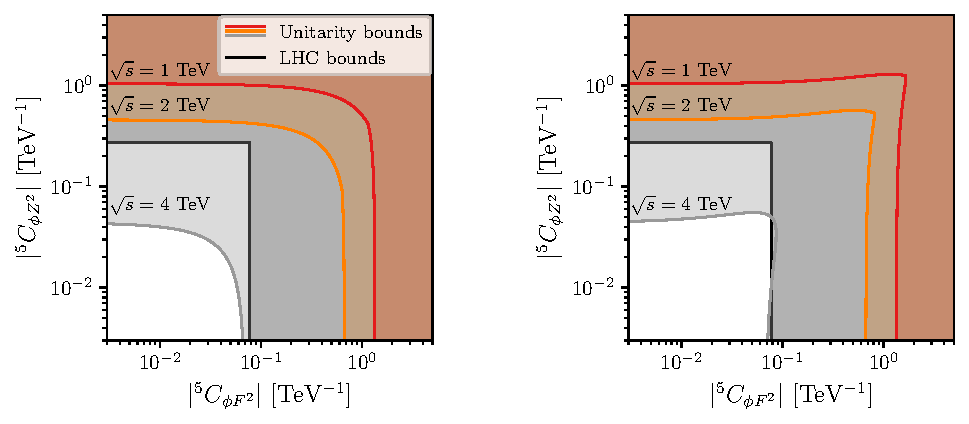
\includegraphics[scale = 0.92]{images/ALPs_gaugebosons.pdf}
    \caption[Unitarity bounds and experimental limits on the axion-like particle couplings to photons and $Z$ bosons]{Parameter space excluded by the partial-wave unitarity bounds in Eq.~\eqref{eq:PWUB_d5_phiX2} for the dimension-five ALP couplings to photons ($\coef{5}{\phi F^2}{} = c^2_{\rm W} \, \coef{5}{\phi B^2}{} + s^2_{\rm W} \,\coef{5}{\phi W^2}{}$) and $Z$ bosons ($\coef{5}{\phi Z^2}{} = s^2_{\rm W} \, \coef{5}{\phi B^2}{} + c^2_{\rm W}\,\coef{5}{\phi W^2}{}$), in the cases where $\coef{5}{\phi F^2}{} \coef{5}{\phi Z^2}{} < 0$ (left panel) and $\coef{5}{\phi F^2}{} \coef{5}{\phi Z^2}{} > 0$ (right panel). In both cases the coupling to gluons has been fixed to $\abs*{\coef{5}{\phi G^2}{}} = 0.225$~TeV$^{-1}$.
    The black region corresponds to the parameter space excluded by Ref.~\cite{Gavela:2019cmq} via non-resonant ALP searches at the LHC, where the limits $\abs*{\coef{5}{\phi F^2}{}\coef{5}{\phi G^2}{}} < 0.018$~TeV$^{-2}$ and $\abs*{\coef{5}{\phi Z^2}{}\coef{5}{\phi G^2}{}} < 0.061$~TeV$^{-2}$ are found for $m_\phi \lesssim 200$~GeV.}
    \label{fig:gaugebosons}
\end{figure}


\subsection{\texorpdfstring{Dimension-Seven Couplings in $l^+ l^- \to \phi h$}{Dimension-Seven Couplings in l+ l- to phi h}}

The relevance of higher-dimensional ALP operators can be nicely illustrated through the process $l^+ l^- \to \phi h$~\cite{Grojean:2023tsd}, which receives contributions from both dimension-five and -seven operators.
In Figure~\ref{fig:crosssection}, we show the cross section for this process in the high-energy limit. The relevant Wilson coefficients are parameterized as $\coef{5}{\phi \ell e H}{ll} = i \, y_l/f$ and $\coef{7}{\phi \ell e H}{(1)ll} = \coef{7}{\phi \ell e H}{(2)ll} = 1/f^3$, where $f$ can be interpreted as the ALP decay constant.

In the high-energy limit, the cross section of $l^+ l^- \to \phi h$ 
is $\sigma = \sigma^{(5)} + \sigma^{(7)}$, where\footnote{The interference term is absent since $\Re{\coef{5}{\phi \ell e H}{ll}\coef{7}{\phi \ell e H}{(1,2)ll}} = 0$ for the benchmark parameterization of the Wilson coefficients.}
%
\begin{equation}
    \sigma^{(7)} = \frac{s^2}{768\pi}\left[\abs{\coef{7}{\phi \ell e H}{(1)ll}}^2+\abs{\coef{7}{\phi \ell e H}{(2)ll}}^2+\Re{\coef{7}{\phi \ell e H}{(1)ll}\,\coef{7}{\phi \ell e H}{(2)ll *}}\right],
\quad
    \sigma^{(5)} = \frac{1}{64\pi}\abs{\coef{5}{\phi \ell e H}{ll}}^2\,.
\end{equation}
%
On the other hand, the partial-wave unitarity bounds lead to the following conditions 
%
\begin{equation}
    \sigma^{(7)} \le \frac{5\pi}{3s}\,,\qquad
    \sigma^{(5)} \le \frac{\pi}{s}\,,
\end{equation}
%
that are illustrated in Figure~\ref{fig:crosssection}.
As a result, large effects to the $l^+ l^- \to \phi h$ cross section can be significantly reduced depending on the ALP decay constant and the center-of-mass energy.
%
\begin{figure}[tb]
    \centering
    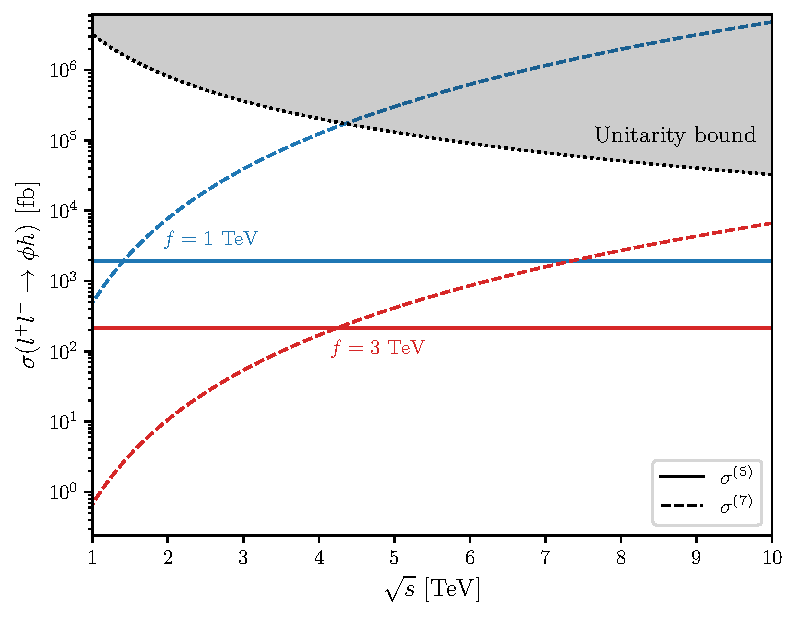
\includegraphics[scale = 0.92]{images/ALPs_crosssection.pdf}
    \caption[High-energy cross section for $l^+l^-\to\phi h$]{Cross section for the process $l^+ l^- \to \phi h$, with $l=e,\mu$, in the high-energy limit. The relevant Wilson coefficients are parameterized as $\coef{5}{\phi \ell e H}{ll} = i \, y_l/f$ and $\coef{7}{\phi \ell e H}{(1)ll} = \coef{7}{\phi \ell e H}{(2)ll} = 1/f^3$, where $f$ can be interpreted as the ALP decay constant.}
    \label{fig:crosssection}
\end{figure}


\subsection{Weak-Violating Axion-Like Particles and Rare Decays}

In the case of weak-violating ALP interacting with electrons (with $\overline g_{ee} = g_{\nu_e} = 0$), the partial-wave unitarity bound reads
%
\begin{equation}
    \abs{g_{ee}} \lesssim 10^{-5} \left(\frac{\text{TeV}}{\sqrt{s}}\right)^2\,.
\end{equation}
%
Instead, in the weak-preserving case (with $\overline g_{ee} = g_{ee}$ and $g_{\nu_e} = 0$), we have
%
\begin{equation}
    \abs{g_{ee}} \lesssim 4 \left(\frac{\text{TeV}}{\sqrt{s}}\right)\,.
\end{equation}

\begin{figure}[tb]
    \centering
    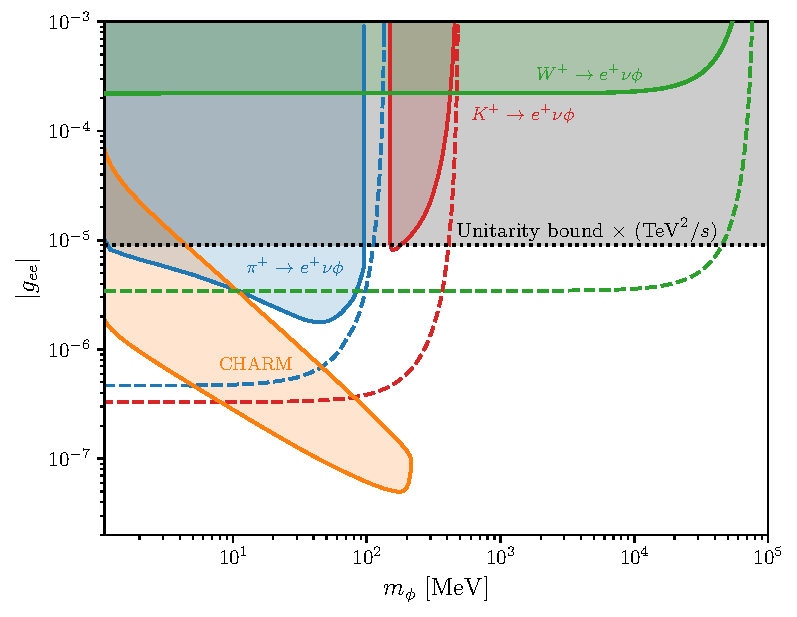
\includegraphics[scale = 0.92]{images/ALPs_WV_gee.pdf}
    \caption[Theoretical and experimental bounds on the weak-violating axion-like particle coupling $g_{ee}$]{Theoretical and experimental bounds on the coupling $g_{ee}$ of a weak-violating ALP~\cite{Altmannshofer:2022ckw}. 
    The partial-wave unitarity bound is shown in grey and scales 
    as $1/s$. 
    Searches for leptonic charged-meson decays are shown in blue (pions)~\cite{PIONEER:2022yag} and red (kaons)~\cite{Poblaguev:2002ug,Altmannshofer:2022ckw}, while searches for rare $W$-boson decays are shown in green~\cite{ParticleDataGroup:2022pth,Altmannshofer:2022ckw}. Bounds from leptonic charged-meson decays in the CHARM proton beam dump~\cite{CHARM:1985anb} are shown in orange~\cite{Altmannshofer:2022ckw}. Dashed lines refer to the potential sensitivities with dedicated searches at the PIONEER experiment~\cite{PIONEER:2022yag} and kaon factories~\cite{Altmannshofer:2022ckw}.}
    \label{fig:WV_gee}
\end{figure}

In order to monitor the impact of the above bounds on physical observables, we consider the branching fractions of $\pi^+\to e^+\nu_e \phi$, $K^+\to e^+\nu_e \phi$, and $W^+\to e^+\nu_e \phi$ decays~\cite{Altmannshofer:2022ckw} in the weak-violating case. 
Neglecting ALP mass effects and taking into account partial-wave unitarity bounds, we find that
%
\begin{align}
    \mathcal B(\pi^+ \to e^+ \nu_e \phi) &\lesssim 4 \times 10^{-9}\left(\frac{\text{TeV}}{\sqrt{s}}\right)^4 \,,
    \\
    \mathcal B(K^+ \to e^+ \nu_e \phi) &\lesssim 7 \times 10^{-8} \left(\frac{\text{TeV}}{\sqrt{s}}\right)^4\,,
    \\
    \mathcal B(W^+ \to e^+ \nu_e \phi) &\lesssim 6 \times 10^{-5} \left(\frac{\text{TeV}}{\sqrt{s}}\right)^4\,.
\end{align}
%
The current bound for the 
$\pi^+ \to e^+ \nu_e \phi$ process arises from the SINDRUM experiment which looked for $e^+e^-$ resonances in $\pi^+ \to e^+ \nu_e \phi$ followed by 
$\phi \to e^+e^-$
with sensitivity to branching ratios of $\mathcal{O}(10^{-10})$~\cite{SINDRUM:1986klz}.
In the future, the PIONEER experiment aims to reach 
the sensitivity of $\mathcal{O}(10^{-11})$~\cite{PIONEER:2022yag}.
Concerning the $K^+ \to e^+ \nu_e \phi$ decay, 
we exploit the E865 search for the SM process 
$K^+ \to e^+ \nu_e e^+e^-$~\cite{Poblaguev:2002ug}. 
Assuming that the ALP channel does not exceed 
twice the uncertainty in this measurement, we impose
the bound $\mathcal{B}(K^+ \to e^+ \nu_e \phi) \leq 4 \times 10^{-9}$~\cite{Altmannshofer:2022ckw}. 
As a future projection, we assume a reference 
bound of $10^{-10}$~\cite{Altmannshofer:2022ckw}.
Moreover, following the analysis of Ref.~\cite{Altmannshofer:2022ckw}, we also impose 
the constraints from leptonic charged meson decays in the CHARM experiment~\cite{CHARM:1985anb}.
As for the $W^+ \to e^+ \nu_e \phi$ decay, we require this mode not to contribute at a visible level to the total width of the $W$ boson
$\Gamma_W = 2.085 \pm 0.042$~GeV~\cite{ParticleDataGroup:2022pth}.
Dedicated analyses for other rare $W$ decays by CMS could improve the bound on the branching ratios of $W^+ \to e^+ \nu_e \phi$ at the level of $10^{-6}$~\cite{Altmannshofer:2022ckw}.

As shown in Figure~\ref{fig:WV_gee}, unitarity bounds already exclude large regions of the parameter space for $\sqrt{s} = 1$~TeV and are typically stronger than the current experimental bounds on charged meson as well as $W$ boson decays.

\section{Conclusions\label{sec:ALPUBconclusions}}

Axion-like particles (ALPs) are generic pseudo-Nambu--Goldstone bosons (pNGBs) emerging from the spontaneous breaking of some global symmetry 
above the electroweak scale. The pNGB nature of ALPs forces their interactions with Standard Model fields to be derivative. Therefore, ALP interactions exhibit an inherent growth with the energy, possibly leading to the breakdown of perturbative unitarity at some large energy scale. 

In this chapter, we have systematically evaluated the partial-wave unitarity bounds for ALP Effective Field Theories (EFTs) including higher-dimensional operators up to dimension eight. The adopted methodology is based on the recently developed formalism described in Chapter~\ref{ch:generalizedUB}, based on on-shell methods, which has proven particularly efficient for studying unitarity bounds of EFTs at high energies~\cite{Bresciani:2025toe}.

In particular, we first revisited and improved the bounds of Ref.~\cite{Brivio:2021fog} relative to dimension-five and -six operators, finding that the processes $XX \to XX$ and $XX \to \phi \phi$ (with $X=B,W,G$) set the most stringent bounds at any energy scale.
The summary of the partial-wave unitarity bounds on the individual
Wilson coefficients associated with these operators is reported in 
Figure~\ref{fig:d56summary}.
Stronger bounds can be obtained through a coupled-channel analysis, 
where several scattering processes such as $BB \to WW$, $WW \to GG$, 
and $BB \to GG$ are generated by the simultaneous presence of different
Wilson coefficients; see Figure~\ref{fig:d5phiX2}.
As a relevant phenomenological application, we discussed the 
impact of the above bounds on non-resonant ALP searches at the LHC~\cite{Gavela:2019cmq}. Unitarity bounds can be competitive or even more stringent than the experimental bounds already for center-of-mass energies at the TeV scale; see Figure~\ref{fig:gaugebosons}. 

Moreover, we discussed partial wave unitarity bounds for dimension-five 
weak-violating ALP interactions; see Figure~\ref{fig:WV}. In this 
case there is a striking energy enhancement $({\rm energy}/m_l)$ 
in several processes such as charged-meson and $W$-boson decays~\cite{Altmannshofer:2022ckw}.
As shown in Figure~\ref{fig:WV_gee}, unitarity bounds exclude large regions of the parameter space already for $\sqrt{s} = 1$~TeV and 
are typically stronger than the current experimental bounds.

Finally, we analyzed the partial-wave unitarity bounds for dimension-seven and -eight operators, which were recently classified in Refs.~\cite{Song:2023lxf,Grojean:2023tsd,Bertuzzo:2023slg}; see
Figures~\ref{fig:d7phipsi2H}, \ref{fig:d7summary}, and \ref{fig:d8summary}.
As a phenomenological application, we considered the process $l^+ l^- \to \phi h$, which receives contributions from both dimension-five and -seven operators, and which can be looked for at future high-energy lepton colliders~\cite{Grojean:2023tsd}. As shown in Figure~\ref{fig:crosssection}, potentially large effects induced by dimension-seven operators are severely reduced depending on the ALP decay constant and the center-of-mass energy.

The last part of this chapter was devoted to the derivation of positivity bounds, stemming from the analyticity and causality of scattering amplitudes, for dimension-eight operators. These were derived from elastic $2 \to 2$ scattering processes that grow with energy as $s^2$.
As shown in Figures~\ref{fig:d8phi2H2} and \ref{fig:d8phi2B2}, positivity and partial-wave unitarity bounds are highly complementary in constraining the parameter space of ALP EFTs. 
Interestingly, our results can also be used to derive new positivity constraints in the SMEFT; see Section~\ref{sec:positivity}.

To conclude, the positivity and partial-wave unitarity bounds derived in this chapter can be applied in several directions, such as ALP searches at colliders, a variety of rare decays, or even as constraints for the event generation, which can impact the shapes of the expected distributions of experimental searches. 
Our work highlights the synergy and interplay of first-principle-based theoretical bounds and experimental limits in our adventure to discover new-physics phenomena.

\begin{subappendices}
    \section{Amplitudes\label{app:ALPUBamplitudes}}

In this appendix we list the relevant amplitudes considered for obtaining the most stringent partial-wave unitarity bounds for the ALP EFT reported in Section~\ref{sec:ALPUBunitarity}.
%
All particles are considered outgoing and massless, since we are interested in the high-energy limit, and the superscripts $\pm$ denote the signs of helicities. 
%
The following notation is used: 
\begin{itemize}
    \item $p,r,\dotsc\in\{1,2,3\}$ are weak-eigenstate indices;
    \item $i,j,\dotsc\in\{1,2\}$ are $SU(2)$ fundamental indices;
    \item $I,J,\dotsc \in \{1,2,3\}$ are $SU(2)$ adjoint indices;
    \item $\alpha,\beta,\dotsc \in\{1,2,3\}$ are $SU(3)$ fundamental indices;
    \item $A,B,\dotsc \in \{1,\dotsc,8\}$ are $SU(3)$ adjoint indices.
\end{itemize}

\subsection{Dimension-Five and -Six Interactions\label{app:amplitudes5e6}}

The relevant amplitudes generated by one or two insertions of dimension-five operators (see Table~\ref{tab:ALPdim5-6}) are 
\begin{align}
\mathcal A(\phi,\ell^-_{ip},\overline e^-_{r},\overline H_j) &= \coef{5}{\phi \ell e H}{pr} \,\agl{2}{3}\delta_{ij} \,, 
\\
\mathcal A(\phi,q^-_{\alpha ip},\overline d^-_{\beta r},\overline H_j) &= \coef{5}{\phi qd H}{pr} \,\agl{2}{3}\delta_{\alpha\beta}\delta_{ij}\,, 
\\
\mathcal A(\phi,q^-_{\alpha ip},\overline u^-_{\beta r}, H_j) &= \coef{5}{\phi qu H}{pr} \,\agl{2}{3}\delta_{\alpha\beta}\epsilon_{ij}\,, 
\\
    \mathcal A(B^+,B^+,B^-,B^-) &= - 4\, \coef{5}{\phi B^2}{2}\,\frac{\agl{3}{4}^2 \sqr{2}{1}}{\agl{1}{2}}\,,  
    \\
    \mathcal A(\phi,\phi,B^-,B^-) &= 8\,\coef{5}{\phi B^2}{2}\,\agl{3}{4}^2\,,
    \\
    \mathcal A(W_I^+,W_J^+,W_K^-,W_L^-) &= - 4\, \coef{5}{\phi W^2}{2}\,\frac{\agl{3}{4}^2 \sqr{2}{1}}{\agl{1}{2}}\delta^{IJ}\delta^{KL}\,, 
    \\
    \mathcal A(W_I^+,W_J^+,W_K^+,W_L^+) &= 4\, \coef{5}{\phi W^2}{2} \bigg[\frac{\sqr{2}{1}\sqr{4}{3}^2}{\agl{1}{2}}\delta^{IJ}\delta^{KL}+\frac{\sqr{3}{1}\sqr{4}{2}^2}{\agl{1}{3}}\delta^{IK}\delta^{JL}\nonumber \\&\quad +\frac{\sqr{4}{1}\sqr{3}{2}^2}{\agl{1}{4}}\delta^{IL}\delta^{JK}\bigg]\,, 
    \\
    \mathcal A(\phi,\phi,W_I^-,W_J^-) &= 8\,\coef{5}{\phi W^2}{2}\,\agl{3}{4}^2 \delta^{IJ}\,,
    \\
    \mathcal A(G_A^+,G_B^+,G_C^-,G_D^-) &= - 4\, \coef{5}{\phi G^2}{2}\,\frac{\agl{3}{4}^2 \sqr{2}{1}}{\agl{1}{2}}\delta^{AB}\delta^{CD}\,, 
    \\
    \mathcal A(G_A^+,G_B^+,G_C^+,G_D^+) &= 4\, \coef{5}{\phi G^2}{2} \bigg[\frac{\sqr{2}{1}\sqr{4}{3}^2}{\agl{1}{2}}\delta^{AB}\delta^{CD}+\frac{\sqr{3}{1}\sqr{4}{2}^2}{\agl{1}{3}}\delta^{AC}\delta^{BD}\nonumber \\&\quad+\frac{\sqr{4}{1}\sqr{3}{2}^2}{\agl{1}{4}}\delta^{AD}\delta^{BC}\bigg] \,, 
    \\
    \mathcal A(\phi,\phi,G_A^-,G_B^-) &= 8\,\coef{5}{\phi G^2}{2}\,\agl{3}{4}^2 \delta^{AB}\,,
    \\
    \mathcal A(B^+,B^+,W_I^-,W_J^-) &= - 4\, \coef{5}{\phi B^2}{}\coef{5}{\phi W^2}{}\,\frac{\agl{3}{4}^2 \sqr{2}{1}}{\agl{1}{2}}\delta^{IJ} \,, 
    \\
    \mathcal A(B^+,B^+,W_I^+,W_J^+) &=  4\, \coef{5}{\phi B^2}{}\coef{5}{\phi W^2}{}\,\frac{\sqr{4}{3}^2 \sqr{2}{1}}{\agl{1}{2}}\delta^{IJ} \,, 
    \\
    \mathcal A(B^+,B^+,G_A^-,G_B^-) &= - 4\, \coef{5}{\phi B^2}{}\coef{5}{\phi G^2}{}\,\frac{\agl{3}{4}^2 \sqr{2}{1}}{\agl{1}{2}}\delta^{AB} \,, 
    \\
    \mathcal A(B^+,B^+,G_A^+,G_B^+) &=  4\, \coef{5}{\phi B^2}{}\coef{5}{\phi G^2}{}\,\frac{\sqr{4}{3}^2 \sqr{2}{1}}{\agl{1}{2}}\delta^{AB} \,, 
    \\
    \mathcal A(W_I^+,W_J^+,G_A^-,G_B^-) &= - 4\, \coef{5}{\phi W^2}{}\coef{5}{\phi G^2}{}\,\frac{\agl{3}{4}^2 \sqr{2}{1}}{\agl{1}{2}}\delta^{IJ}\delta^{AB} \,, 
    \\
    \mathcal A(W_I^+,W_J^+,G_A^+,G_B^+) &=  4\, \coef{5}{\phi W^2}{}\coef{5}{\phi G^2}{}\,\frac{\sqr{4}{3}^2 \sqr{2}{1}}{\agl{1}{2}}\delta^{IJ}\delta^{AB}\,.
\end{align}

The relevant amplitude generated by the only dimension-six operator (see Table~\ref{tab:ALPdim5-6}) is 
\begin{equation}
    \mathcal A(\phi,\phi,H_i,\overline H_j) = -\coef{6}{\phi^2 H^2}{} \,\agl{1}{2}\sqr{2}{1}\delta_{ij}\,.
\end{equation}

\subsection{Dimension-Seven Interactions}

The relevant amplitudes generated by one insertion of dimension-seven operators (see Table~\ref{tab:ALPdim7}) are 
\begin{align}
    \mathcal A(\phi,\ell^-_{ip},\overline e_r^-,\overline H_j)&=-\frac{1}{2}\left(\coef{7}{\phi \ell e H}{(1)pr} \, \agl{1}{3}\sqr{3}{1} + \coef{7}{\phi \ell e H}{(2)pr} \, \agl{1}{2}\sqr{2}{1}\right)\agl{2}{3}\delta_{ij}\,,
    \\
    \mathcal A(\phi,q^-_{\alpha ip},\overline d_{\beta r}^-,\overline H_j)&=-\frac{1}{2}\left(\coef{7}{\phi qd H}{(1)pr} \, \agl{1}{3}\sqr{3}{1} + \coef{7}{\phi qd H}{(2)pr} \, \agl{1}{2}\sqr{2}{1}\right)\agl{2}{3}\delta_{\alpha\beta}\delta_{ij}\,,
    \\
    \mathcal A(\phi,q^-_{\alpha ip},\overline u_{\beta r}^-, H_j)&=-\frac{1}{2}\left(\coef{7}{\phi qu H}{(1)pr} \, \agl{1}{3}\sqr{3}{1} + \coef{7}{\phi qu H}{(2)pr} \, \agl{1}{2}\sqr{2}{1}\right)\agl{2}{3}\delta_{\alpha\beta}\epsilon_{ij}\,,
    \\
    \mathcal A(\phi,\ell_{ip}^-,\overline \ell_{jr}^+,B^-) &= \frac{1}{\sqrt{2}}\left(\coef{7}{\phi \ell^2 B}{(1)pr} + i\,\coef{7}{\phi \ell^2 B}{(2)pr}\right) \agl{1}{4}\agl{2}{4}\sqr{3}{1}\delta_{ij} \,,
    \\
    \mathcal A(\phi,e_{p}^+,\overline e_{r}^-,B^-) &= \frac{1}{\sqrt{2}}\left(\coef{7}{\phi e^2 B}{(1)pr} + i\,\coef{7}{\phi e^2 B}{(2)pr}\right) \agl{1}{4}\agl{3}{4}\sqr{2}{1} \,,
    \\
    \mathcal A(\phi,q_{\alpha ip}^-,\overline q_{\beta jr}^+,B^-) &= \frac{1}{\sqrt{2}}\left(\coef{7}{\phi q^2 B}{(1)pr} + i\,\coef{7}{\phi q^2 B}{(2)pr}\right) \agl{1}{4}\agl{2}{4}\sqr{3}{1}\delta_{\alpha\beta}\delta_{ij} \,,
    \\
    \mathcal A(\phi,u_{\alpha p}^+,\overline u_{\beta r}^-,B^-) &= \frac{1}{\sqrt{2}}\left(\coef{7}{\phi u^2 B}{(1)pr} + i\,\coef{7}{\phi u^2 B}{(2)pr}\right) \agl{1}{4}\agl{3}{4}\sqr{2}{1}\delta_{\alpha\beta} \,,
    \\
    \mathcal A(\phi,d_{\alpha p}^+,\overline d_{\beta r}^-,B^-) &= \frac{1}{\sqrt{2}}\left(\coef{7}{\phi d^2 B}{(1)pr} + i\,\coef{7}{\phi d^2 B}{(2)pr}\right) \agl{1}{4}\agl{3}{4}\sqr{2}{1}\delta_{\alpha\beta} \,,
    \\
    \mathcal A(\phi,\ell_{ip}^-,\overline \ell_{jr}^+,W_I^-) &= \frac{1}{\sqrt{2}}\left(\coef{7}{\phi \ell^2 W}{(1)pr} + i\,\coef{7}{\phi \ell^2 W}{(2)pr}\right) \agl{1}{4}\agl{2}{4}\sqr{3}{1}\sigma^I_{ij} \,,
    \\
    \mathcal A(\phi,q_{\alpha ip}^-,\overline q_{\beta jr}^+,W_I^-) &= \frac{1}{\sqrt{2}}\left(\coef{7}{\phi q^2 W}{(1)pr} + i\,\coef{7}{\phi q^2 W}{(2)pr}\right) \agl{1}{4}\agl{2}{4}\sqr{3}{1}\delta_{\alpha\beta}\sigma^I_{ij} \,,
    \\
    \mathcal A(\phi,q_{\alpha ip}^-,\overline q_{\beta jr}^+,G_A^-) &= \frac{1}{\sqrt{2}}\left(\coef{7}{\phi q^2 G}{(1)pr} + i\,\coef{7}{\phi q^2 G}{(2)pr}\right) \agl{1}{4}\agl{2}{4}\sqr{3}{1}\lambda^A_{\alpha\beta}\delta_{ij} \,,
    \\
    \mathcal A(\phi,u_{\alpha p}^+,\overline u_{\beta r}^-,G_A^-) &= \frac{1}{\sqrt{2}}\left(\coef{7}{\phi u^2 G}{(1)pr} + i\,\coef{7}{\phi u^2 G}{(2)pr}\right) \agl{1}{4}\agl{3}{4}\sqr{2}{1}\lambda^A_{\alpha\beta} \,,
    \\
    \mathcal A(\phi,d_{\alpha p}^+,\overline d_{\beta r}^-,G_A^-) &= \frac{1}{\sqrt{2}}\left(\coef{7}{\phi d^2 G}{(1)pr} + i\,\coef{7}{\phi d^2 G}{(2)pr}\right) \agl{1}{4}\agl{3}{4}\sqr{2}{1}\lambda^A_{\alpha\beta} \,,
    \\
    \mathcal A(\phi,H_i,\overline H_j,B^-) &= \frac{1}{2\sqrt{2}}\left(\coef{7}{\phi B H^2}{(1)} + i \,\coef{7}{\phi B H^2}{(2)}\right)\agl{1}{4}(\agl{2}{4}\sqr{2}{1}-\agl{3}{4}\sqr{3}{1})\delta_{ij}\,,
    \\
    \mathcal A(\phi,H_i,\overline H_j,W_I^-) &= \frac{1}{2\sqrt{2}}\left(\coef{7}{\phi W H^2}{(1)} + i \,\coef{7}{\phi W H^2}{(2)}\right)\agl{1}{4}(\agl{2}{4}\sqr{2}{1}-\agl{3}{4}\sqr{3}{1})\sigma^I_{ij}\,,
    \\
    \mathcal A(\phi,H_i,\overline H_j,H_k,\overline H_l) &= \frac{i}{2}\,\coef{7}{\phi H^4}{}\left(-\agl{1}{2}\sqr{2}{1}+\agl{1}{3}\sqr{3}{1}-\agl{1}{4}\sqr{4}{1}+\agl{1}{5}\sqr{5}{1}\right)\nonumber \\
    &\quad \times (\delta_{ij}\delta_{kl}+\delta_{il}\delta_{kj})\,,
    \\
    \mathcal A(\phi, e^+_p,\overline e^-_r, H_i,\overline H_j) &= i\,\coef{7}{\phi e^2 H^2}{pr}\,\agl{1}{3}\sqr{2}{1}\delta_{ij}\,,
    \\
    \mathcal A(\phi, u^+_{\alpha p},\overline u^-_{\beta r}, H_i,\overline H_j) &= i\,\coef{7}{\phi u^2 H^2}{pr}\,\agl{1}{3}\sqr{2}{1}\delta_{\alpha\beta}\delta_{ij}\,,
    \\
    \mathcal A(\phi, d^+_{\alpha p},\overline d^-_{\beta r}, H_i,\overline H_j) &= i\,\coef{7}{\phi d^2 H^2}{pr}\,\agl{1}{3}\sqr{2}{1}\delta_{\alpha\beta}\delta_{ij}\,,
    \\
    \mathcal A (\phi,\ell^-_{ip},\overline \ell^+_{jr},H_k,\overline H_l) &= i\left[\left(\coef{7}{\phi \ell^2 H^2}{(1)pr}-\coef{7}{\phi \ell^2 H^2}{(2)pr}\right)\delta_{ij}\delta_{kl}+2\,\coef{7}{\phi \ell^2 H^2}{(2)pr}\,\delta_{il}\delta_{kj}\right]\agl{1}{2}\sqr{3}{1}\,,
    \\
    \mathcal A (\phi,q^-_{\alpha ip},\overline q^+_{\beta jr},H_k,\overline H_l) &= i\left[\left(\coef{7}{\phi q^2 H^2}{(1)pr}-\coef{7}{\phi q^2 H^2}{(2)pr}\right)\delta_{ij}\delta_{kl}+2\,\coef{7}{\phi q^2 H^2}{(2)pr}\,\delta_{il}\delta_{kj}\right]\agl{1}{2}\sqr{3}{1}\delta_{\alpha\beta}\,.
\end{align}

\subsection{Dimension-Eight Interactions}

The relevant amplitudes generated by one insertion of dimension-eight operators (see Table~\ref{tab:ALPdim8}) are 
\begin{align}
    \mathcal A(\phi,\phi,\phi,\phi) &= 2\,\coef{8}{\phi^4}{}\,(\agl{1}{2}^2\sqr{2}{1}^2 + \agl{1}{3}^2\sqr{3}{1}^2 + \agl{1}{4}^2\sqr{4}{1}^2)\,,
    \\
    \mathcal A(\phi,\phi,H_i,\overline H_j,H_k,\overline H_l) &= -2\,\coef{8}{\phi^2 H^4}{}\,\agl{1}{2}\sqr{2}{1}(\delta_{ij}\delta_{kl}+\delta_{il}\delta_{kj})\,,
    \\
    \mathcal A(\phi,\phi,H_i,\overline H_j) &= \frac{1}{2}\,\coef{8}{\phi^2 H^2}{(1)}\,\agl{1}{2}^2\sqr{2}{1}^2 + \frac{1}{4}\,\coef{8}{\phi^2 H^2}{(2)}\,(\agl{1}{3}^2\sqr{3}{1}^2 + \agl{1}{4}^2\sqr{4}{1}^2)\,,
    \\
    \mathcal A(\phi,\phi,B^-,B^-) &= 2\left(\frac{1}{4}\,\coef{8}{\phi^2 B^2}{(1)}+\coef{8}{\phi^2 B^2}{(2)} + i\,\coef{8}{\phi^2 B^2}{(3)}\right)\agl{3}{4}^3 \sqr{4}{3}\,,
    \label{eq:ampl_d8_phi2B2(1)}
    \\
    \mathcal A(\phi,\phi,B^-,B^+) &= \coef{8}{\phi^2 B^2}{(1)}\,\agl{1}{3}^2\sqr{4}{1}^2\,,
    \label{eq:ampl_d8_phi2B2(2)}
    \\
    \mathcal A(\phi,\phi,W_I^-,W_J^-) &= 2\left(\frac{1}{4}\,\coef{8}{\phi^2 W^2}{(1)}+\coef{8}{\phi^2 W^2}{(2)} + i\,\coef{8}{\phi^2 W^2}{(3)}\right)\agl{3}{4}^3 \sqr{4}{3}\delta^{IJ}\,,
    \\
    \mathcal A(\phi,\phi,W_I^-,W_J^+) &= \coef{8}{\phi^2 W^2}{(1)}\,\agl{1}{3}^2\sqr{4}{1}^2\delta^{IJ} \,,
    \\
    \mathcal A(\phi,\phi,G_A^-,G_B^-) &= 2\left(\frac{1}{4}\,\coef{8}{\phi^2 G^2}{(1)}+\coef{8}{\phi^2 G^2}{(2)} + i\,\coef{8}{\phi^2 G^2}{(3)}\right)\agl{3}{4}^3 \sqr{4}{3}\delta^{AB}\,,
    \\
    \mathcal A(\phi,\phi,G_A^-,G_B^+) &= \coef{8}{\phi^2 G^2}{(1)}\,\agl{1}{3}^2\sqr{4}{1}^2 \delta^{AB} \,,
    \\
    \mathcal A(\phi,\phi,\ell^-_{ip},\overline \ell^+_{jr}) &= \frac{1}{2}\,\coef{8}{\phi^2 \ell^2}{pr}\left(\agl{1}{3}\agl{1}{4}\sqr{4}{1}^2 + \agl{2}{3}\agl{2}{4}\sqr{4}{2}^2\right)\delta_{ij}\,,
    \\
    \mathcal A(\phi,\phi,e^+_p,\overline e^-_r) &= \frac{1}{2}\,\coef{8}{\phi^2 e^2}{pr}\left(\agl{1}{3}\agl{1}{4}\sqr{3}{1}^2 + \agl{2}{3}\agl{2}{4}\sqr{3}{2}^2\right)\,,
    \\
    \mathcal A(\phi,\phi,q^-_{\alpha ip},\overline q^+_{\beta jr}) &= \frac{1}{2}\,\coef{8}{\phi^2 q^2}{pr}\left(\agl{1}{3}\agl{1}{4}\sqr{4}{1}^2 + \agl{2}{3}\agl{2}{4}\sqr{4}{2}^2\right)\delta_{\alpha\beta}\delta_{ij}\,,
    \\
    \mathcal A(\phi,\phi,u^+_{\alpha p},\overline u^-_{\beta r}) &= \frac{1}{2}\,\coef{8}{\phi^2 u^2}{pr}\left(\agl{1}{3}\agl{1}{4}\sqr{3}{1}^2 + \agl{2}{3}\agl{2}{4}\sqr{3}{2}^2\right)\delta_{\alpha\beta}\,,
    \\
    \mathcal A(\phi,\phi,d^+_{\alpha p},\overline d^-_{\beta r}) &= \frac{1}{2}\,\coef{8}{\phi^2 d^2}{pr}\left(\agl{1}{3}\agl{1}{4}\sqr{3}{1}^2 + \agl{2}{3}\agl{2}{4}\sqr{3}{2}^2\right)\delta_{\alpha\beta}\,,
    \\
    \mathcal A(\phi,\phi,\ell^-_{ip},\overline e^-_{r},\overline H_j) &= -\coef{8}{\phi^2\ell e H}{pr}\,\agl{1}{2}\agl{3}{4}\sqr{2}{1}\delta_{ij}\,,
    \\
    \mathcal A(\phi,\phi,q^-_{\alpha ip},\overline d^-_{\beta r},\overline H_j) &= -\coef{8}{\phi^2qd H}{pr}\,\agl{1}{2}\agl{3}{4}\sqr{2}{1}\delta_{\alpha\beta}\delta_{ij}\,,
    \\
    \mathcal A(\phi,\phi,q^-_{\alpha ip},\overline u^-_{\beta r}, H_j) &= -\coef{8}{\phi^2qu H}{pr}\,\agl{1}{2}\agl{3}{4}\sqr{2}{1}\delta_{\alpha\beta}\epsilon_{ij}\,.
\end{align}
    \chapter{Positivity Bounds in an Ultraviolet Extension\label{app:UVext}}

To test the validity of the positivity bounds presented in Section~\ref{sec:positivity}, we match a UV theory to the ALP EFT.
A simple way to generate at tree level the operators subject to the positivity constraints consists in integrating out a massive spin-2 field $h_{\mu\nu}$ \textit{minimally} coupled to the stress-energy tensor $T_{\mu\nu}$ \cite{Fierz:1939ix,Hinterbichler:2011tt}:
\begin{equation}
    \mathcal L = \frac{1}{2}\partial_\lambda h_{\mu\nu}\partial^\lambda h^{\mu\nu}-\partial_\mu h_{\nu\lambda}\partial^\nu h^{\mu\lambda} +\partial_\mu h^{\mu\nu}\partial_\nu h-\frac{1}{2}\partial_\lambda h  \partial^\lambda h-\frac{M^2}{2}(h_{\mu\nu}h^{\mu\nu}-h^2)
    +\frac{c}{\Lambda}h^{\mu\nu}T_{\mu\nu}
\end{equation}
where $h=h^\mu_\mu$ is the trace of the field, $c$ is a real dimensionless coefficient, and $\Lambda$ is an energy scale much higher than the ALP EFT cutoff scale. Regarding the stress-energy tensor, we can consider
\begin{equation}
    T_{\mu\nu} = T_{\mu\nu}^{(\phi)} + T_{\mu\nu}^{(H)} + \sum_{\psi = \ell, e , q, u, d} T_{\mu\nu}^{(\psi)} + \sum_{X=B,W,G} T_{\mu\nu}^{(X)}
\end{equation}
with
\begin{align}
    T_{\mu\nu}^{(\phi)} &= \partial_\mu \phi \, \partial_\nu \phi - \frac{1}{2}g_{\mu\nu}\partial_\rho \phi \, \partial^\rho \phi\,,\label{eq:set_phi}\\
    T_{\mu\nu}^{(H)} &= D_\mu H^\dagger D_\nu H + D_\nu H^\dagger D_\mu H - g_{\mu\nu}D_\rho H^\dagger D^\rho H\,,\label{eq:set_higgs}\\
    T^{(\psi)}_{\mu\nu} &= \kappa^{(\psi)}_{pr}\left[\frac{i}{4}\left( \overline \psi_p \gamma_\mu \overset{\leftrightarrow}{D}_\nu \psi_r+\overline \psi_p \gamma_\nu \overset{\leftrightarrow}{D}_\mu \psi_r\right) -  g_{\mu\nu} \overline \psi_p i\slashed{D} \psi_r\right]\,,\\
    T^{(X)}_{\mu\nu} &= -X^{\mathscr A}_{\mu\rho} X_\nu^{\mathscr A \rho} + \frac{1}{4}g_{\mu\nu} X^{\mathscr A}_{\rho\sigma}X^{\mathscr A \rho\sigma}\,.
\end{align}
The matrices $\kappa^{(\psi)}$ must be Hermitian and positive definite ($\kappa^{(\psi)} \succ 0$) to ensure that unitarity is not violated.

Integrating out at tree level $h_{\mu\nu}$, we generate dimension-eight operators that belong both to the SMEFT and to the ALP EFT.
Concerning the latter, the associated Wilson coefficients take the following values:
\begin{gather}
    \coef{8}{\phi^4}{} =\frac{1}{3}\left( \frac{c}{\Lambda M}\right)^2\,,
    \\
    \coef{8}{\phi^2 H^2}{(1)} =-\frac{2}{3}\left( \frac{c}{\Lambda M}\right)^2\,, \qquad \coef{8}{\phi^2 H^2}{(2)} =2\left( \frac{c}{\Lambda M}\right)^2\,,
    \\
    \coef{8}{\phi^2 X^2}{(1)} =-\left( \frac{c}{\Lambda M}\right)^2\,, \quad 
    \coef{8}{\phi^2 X^2}{(2)} =\frac{1}{4}\left( \frac{c}{\Lambda M}\right)^2\,,\quad 
    \coef{8}{\phi^2 X^2}{(3)} =0 \,,
    \quad X=B,W,G\,,
    \\
    \coef{8}{\phi^2 \psi^2}{pr} =\kappa^{(\psi)}_{pr}\left( \frac{c}{\Lambda M}\right)^2\,,
    \qquad \psi = \ell,e,q,u,d\,.
\end{gather}
All of them are consistent with the positivity constraints of Section~\ref{sec:positivity}.

The same conclusion holds if $h_{\mu\nu}$ is \textit{conformally} coupled, which consists in substituting the expressions for $T_{\mu\nu}^{(\phi)}$ and $T_{\mu\nu}^{(H)}$ in Eqs.~\eqref{eq:set_phi} and \eqref{eq:set_higgs} with the improved traceless combinations~\cite{Callan:1970ze}
\begin{align}
    T_{\mu\nu}^{(\phi)} &= \partial_\mu \phi \, \partial_\nu \phi - \frac{1}{2}g_{\mu\nu}\partial_\rho \phi \, \partial^\rho \phi - \frac{1}{6}(\partial_\mu \partial_\nu - g_{\mu\nu}\partial_\rho \partial^\rho)\phi^2\,,\\
    T_{\mu\nu}^{(H)} &= D_\mu H^\dagger D_\nu H + D_\nu H^\dagger D_\mu H - g_{\mu\nu}D_\rho H^\dagger D^\rho H \nonumber \\ &\quad - \frac{1}{6}(D_\mu D_\nu+D_\nu D_\mu -2 g_{\mu\nu}D_\rho D^\rho)(H^\dagger H)\,,
\end{align}
respectively.
With respect to the previous case, none of the Wilson coefficients change value, and the effective Lagrangian remains consistent with the positivity bounds.
\end{subappendices}

\chapter{Unitarity and Sum-Rule Bounds in the Standard Model Effective Field Theory\label{ch:SMEFT_bounds}}

\begin{flushright}
\small

{\color{chapterpaperrule}\rule{\textwidth}{0.5pt}}

\textit{This chapter is based on Ref.~\cite{Bresciani:2026acy}:}\\[0.5em]
L.~C.~Bresciani, P.~Paradisi and A.~Sainaghi,\\[0pt]
``Unitarity bounds and sum rules in the SMEFT,''\\[0pt]
[\href{https://doi.org/10.48550/arXiv.2603.03423}{arXiv:2603.03423} [hep-ph]].

{\color{chapterpaperrule}\rule{\textwidth}{0.5pt}}
\end{flushright}

\section{Introduction}

The discovery of a scalar particle consistent with the SM Higgs boson at the LHC has firmly
established the validity of the SM. Since no experimental data at present significantly contradict
the SM predictions, it is customary to assume the emergence of new physics at energies much above the
electroweak scale. In this context, EFTs provide a systematic framework to parameterize possible
deviations from the SM by introducing higher-dimensional operators constructed from the SM fields and
respecting its symmetries, namely the
SMEFT~\cite{Buchmuller:1985jz,Grzadkowski:2010es,Brivio:2017vri,Isidori:2023pyp,Aebischer:2025qhh}.

As discussed in Chapter~\ref{ch:generalizedUB}, a key theoretical consistency requirement for any theory
is perturbative unitarity, derived from the fundamental properties of the scattering
$S$-matrix~\cite{Jacob:1959at}. The resulting bounds are inherently perturbative, being derived at
tree level, and therefore do not represent sharp exclusions. Their saturation signals the breakdown
of the low-energy description, indicating the energy scale at which new degrees of freedom or a
strongly coupled regime must appear.

Partial-wave unitarity bounds within the SMEFT have already been partially explored in the
literature. In particular, Refs.~\cite{Corbett:2014ora,Corbett:2017qgl,Cao:2023qks} considered
dimension-six bosonic operators and two-fermion-two-boson operators, but restricted the analysis to
operators without gluon fields. In these works, four-fermion operators were not considered. Earlier
studies addressed unitarity in specific four-fermion interactions~\cite{Anders:1993dk}, but a
systematic SMEFT treatment was still lacking. Moreover, dimension-six operators $\psi^2\varphi^3$
modifying the Yukawa interactions were neglected, and no unitarity bounds were derived for the Higgs
operator $(\varphi^\dagger \varphi)^3$.
In this chapter we fill these gaps by providing the first complete coupled-channel implementation of
perturbative unitarity for the baryon-number-conserving dimension-six SMEFT. To this end, we compute
all relevant scattering amplitudes including every allowed helicity, gauge, and flavor configuration,
consistently retaining the correlations among Wilson coefficients entering the same partial-wave
amplitudes. We then marginalize over each Wilson coefficient. This is especially relevant in flavor
scenarios with dominant couplings to third-generation fermions, as naturally realized in models
addressing the flavor puzzle at the TeV scale, which have attracted considerable interest in the
recent
literature~\cite{Bordone:2017bld,Greljo:2018tuh,Allwicher:2020esa,Fuentes-Martin:2020bnh,%
Fuentes-Martin:2022xnb,Barbieri:2023qpf,Barbieri:2024zkh,Davighi:2023evx,Davighi:2023iks,%
Fuentes-Martin:2024fpx,Covone:2024elw,Lizana:2024jby,FernandezNavarro:2023rhv,%
FernandezNavarro:2024hnv,FernandezNavarro:2025zmb,Isidori:2025rci,Greljo:2025mwj}.

The analyticity of the $S$-matrix allows one to derive spin-dependent sum
rules~\cite{Low:2009di,Altmannshofer:2023bfk,Altmannshofer:2025lun,Gu:2020thj,Azatov:2021ygj,%
Remmen:2020uze,Remmen:2022orj}, providing additional theoretical constraints on effective
four-fermion interactions beyond the partial-wave unitarity bounds. Remarkably, the resulting pattern
of SMEFT inequalities can be used to infer characteristic features of the underlying new-physics
dynamics, indicating whether it is dominated by scalar or vector states. A further goal of this
chapter is therefore to explore the complementarity of unitarity and sum-rule constraints, as well as
their competitiveness with both current and projected experimental limits.

In the high-energy particle physics community, there is a growing consensus on performing
new-physics searches with minimal theoretical priors. The huge and otherwise unmanageable parameter
space must be supplemented by restrictive, yet general, first-principles criteria to make such
searches tractable. In this context, the results of this chapter provide a systematic consistency
framework that can be directly incorporated into present and future global SMEFT analyses.

The chapter is organized as follows. In Section~\ref{sec:SMEFT_unitaritybounds} we apply the method
of Chapter~\ref{ch:generalizedUB} to the dimension-six SMEFT and collect the marginalized bounds on
the complete set of Wilson coefficients in the single-flavor limit. In
Section~\ref{sec:SMEFT_sumrules} we derive the spinning sum rules for four-fermion operators in the
Warsaw basis, describing how they are turned into inequalities on the Wilson coefficients and under
which conditions they may fail. In Section~\ref{sec:SMEFT_multiflavor} we present the bounds on four-fermion operators under the MFV and $U(2)^5$ flavor
hypotheses. Section~\ref{sec:SMEFT_pheno} is dedicated to the phenomenological applications of our
results and to their interplay with current and projected experimental limits. Our conclusions are
presented in Section~\ref{sec:SMEFT_conclusions}. Finally, Appendix~\ref{app:SMEFT_conv} collects the
operator basis and our conventions, Appendix~\ref{app:SMEFT_UV} matches a representative set of
UV completions onto the semileptonic operators, Appendix~\ref{app:SMEFT_math} gathers the
mathematical tools used in the derivation of the bounds, and Appendix~\ref{app:SMEFT_flavorresults}
reports the complete set of bounds on the flavorful four-fermion operators.

\section{Unitarity Bounds\label{sec:SMEFT_unitaritybounds}}

To compute the unitarity bounds, we adopt the method developed in Chapter~\ref{ch:generalizedUB}, which allows one to project a generic scattering amplitude $\ket*{\mathcal{A}_{i\to f}}$ onto a kinematic basis $\ket*{\mathcal{B}^J_{i\to f}}$ with definite angular momentum $J$, as follows:
\begin{equation}
\ket*{\mathcal{A}_{i\to f}}=\sum_J a_{i\to f}^J \ket*{\mathcal{B}_{i\to f}^J}\,,
\end{equation}
where $a_{i\to f}^J$ denote the partial-wave coefficients and the elements of the kinematic basis are normalized as 
\begin{equation}
    \langle \mathcal B^J_{i\to f}|\mathcal B^{J'}_{i\to f}\rangle = \int \dd\Phi_i \dd\Phi_f \, \mathcal B^{J'}_{i\to f} \left(\mathcal B^J_{i\to f}\right)^* = (2J+1)\delta^{JJ'}\,,
\end{equation}
where $\dd\Phi_{i,f}$ refers to the phase-space measure associated with the initial and final states.
In terms of $a_{i\to f}^J$, the partial-wave unitarity bounds 
take the form
%
\begin{equation}\label{unitarity bound general}
\abs*{\Re a_{i\to i}^J}\leq 1\,,
\quad
0\leq \Im a_{i\to i}^J\leq 2\,,
\quad
\abs*{a_{i\to f}^J}\leq 1\,,
\end{equation}
with $i \neq f$.
Further details on the construction of the basis and on the derivation of these bounds have been given in Chapter~\ref{ch:generalizedUB}.

Using this framework, we systematically computed the partial-wave unitarity bounds 
for all dimension-six SMEFT Wilson coefficients in the Warsaw basis \cite{Grzadkowski:2010es}, reported in Appendix~\ref{app:SMEFT_conv} with the relevant conventions. 
The resulting bounds in the single-flavor limit are summarized in Table~\ref{tab:UniBounds}.

\begin{table}[h!t!b]
\renewcommand{\arraystretch}{1.5}
    \centering
    \resizebox{\textwidth}{!}{
    \begin{tabular}{c|c|c|c|c|c|c|c|c|c}
    \toprule
    \rowcolor{hdrcolor}
    \multicolumn{2}{c|}{{\boldmath$X^3$}} & \multicolumn{2}{c|}{{\boldmath$\varphi^6$} and {\boldmath$\varphi^4D^2$}} & \multicolumn{2}{c|}{{\boldmath$   \psi^2\varphi^3$}} & \multicolumn{2}{c|}{{\boldmath$(\overline{L}L)(\overline{L}L)$}} & \multicolumn{2}{c}{{\boldmath$(\overline{L}R)(\overline{R}L)$} and {\boldmath$(\overline{L}R)(\overline{L}R)$}}\\
    \hline
    $C_G$ & $4\pi/(9g_s)$ & $C_\varphi$ & $32\pi^3/3$ & $C_{e\varphi}$ & $32\pi^2/\sqrt{3}$ & $C_{\ell\ell}$ & $2\pi$ & $C_{\ell e dq}$ & $8\pi/\sqrt{3}$ \\
    
    $C_{\widetilde G}$ & $4\pi/(9g_s)$ & $C_{\varphi\Box}$ & $8\pi/3$ & $C_{u\varphi}$ & $32\pi^2/3$ & $C_{qq}^{(1)}$ & $6\pi/5$ & $C_{quqd}^{(1)}$ & $16\pi(1+\sqrt{2})/9$\\ 
        
    $C_W$ & $2\pi/(3g)$ &$C_{\varphi D}$ & $32\pi/3$ & $C_{d\varphi}$ & $32\pi^2/3$ & $C_{qq}^{(3)}$ & $4\pi/3$ & $C_{quqd}^{(8)}$ & $4\pi(2+7\sqrt{2})/3$\\
    
    $C_{\widetilde W}$ & $2\pi/(3g)$ & & & & & $C_{\ell q}^{(1)}$ & $2\pi\sqrt{3}$ & $C_{\ell equ}^{(1)}$ & $8\pi/\sqrt{3}$ \\

    &&&&&&  $C_{\ell q}^{(3)}$ & $2\pi$ & $C_{\ell e qu}^{(3)}$ & $(2+\sqrt{2})\pi/3$   \\
    
         \midrule
         \rowcolor{hdrcolor}
         \multicolumn{2}{c|}{{\boldmath$X^2\varphi^2$}} & \multicolumn{2}{c|}{{\boldmath$\psi^2 X \varphi$}} & \multicolumn{2}{c|}{{\boldmath$\psi^2\varphi^2D$}} & \multicolumn{2}{c|}{{\boldmath$(\overline{R}R)(\overline{R}R)$}} & \multicolumn{2}{c}{{\boldmath$(\overline{L}L)(\overline{R}R)$}}\\
         \hline
         $C_{\varphi G}$ & $\pi$ & $C_{eW}$ & $4\pi\sqrt{2/3}$ & $C_{\varphi \ell}^{(1)}$ & $8\pi$ & $C_{ee}$ & $2\pi$ & $C_{\ell e}$ & $4\pi$ \\
         
         $C_{\varphi \widetilde G}$ & $\pi$ & $C_{eB}$ & $4\pi$ & $C_{\varphi \ell}^{(3)}$ & $8\pi/3$ & $C_{uu}$ & $3\pi/2$ & $C_{\ell u}$ & $4\pi$\\
         
         $C_{\varphi W}$ & $2\pi\sqrt{2/3}$ & $C_{uG}$ & $2\pi\sqrt{3}$ & $C_{\varphi e}$ & $8\pi$ & $C_{dd}$ & $3\pi/2$ & $C_{\ell d}$ & $4\pi$\\
         
         $C_{\varphi \widetilde W}$ & $2\pi\sqrt{2/3}$ & $C_{uW}$ & $4\pi\sqrt{2/3}$ & $C_{\varphi q}^{(1)}$ & $2\pi\sqrt{6}$ & $C_{eu}$ & $4\pi$ & $C_{q e}$ & $4\pi$ \\
         
        $C_{\varphi B}$ & $2\pi\sqrt{2}$ & $C_{uB}$ & $4\pi$ & $C_{\varphi q}^{(3)}$ & $8\pi/3$ & $C_{ed}$ & $4\pi$ & $C_{q u}^{(1)}$ & $2\pi\sqrt{2}$\\
        
        $C_{\varphi \widetilde B}$ & $2\pi\sqrt{2}$ & $C_{dG}$ & $2\pi\sqrt{3}$ & $C_{\varphi u}$ & $4\pi \sqrt{3}$ & $C_{ud}^{(1)}$ & $4\pi$ & $C_{q u}^{(8)}$ & $3\pi(1+1/\sqrt{2})$\\
        
        $C_{\varphi W B}$ & $4\pi$ & $C_{dW}$ & $4\pi\sqrt{2/3}$ & $C_{\varphi d}$ & $4\pi\sqrt{3}$ & $C_{ud}^{(8)}$ & $8\pi$ & $C_{qd}^{(1)}$ & $2\pi\sqrt{2}$\\
        
        $C_{\varphi \widetilde W B}$ & $4\pi$ & $C_{dB}$ & $4\pi$ & $C_{\varphi ud}$ & $8\pi$ & & & $C_{q d}^{(8)}$ & $3\pi(1+1/\sqrt{2})$ \\
        \bottomrule
    \end{tabular}
    }
    \caption{Unitarity bounds on the modulus of the baryon-number-conserving dimension-six SMEFT Wilson coefficients in the Warsaw basis \cite{Grzadkowski:2010es} (see Table \ref{tab:WarsawBasis}), obtained by marginalizing over all other SMEFT coefficients. The factors $s/\Lambda^2$ are left implicit, i.e., the reported values constrain the combination $s|C|/\Lambda^2$. Fermionic operators correspond to the single-flavor limit.}
    \label{tab:UniBounds}
\end{table}

Several comments are in order. 
In contrast to the common practice in SMEFT analyses, where only one or a few operators are considered at a time, the unitarity bound associated with each Wilson coefficient is obtained by marginalizing over all other SMEFT coefficients. 
In practice, the marginalized bound on each coefficient is its largest value allowed by unitarity with all remaining coefficients free to vary. Since the partial-wave coefficients depend linearly on the Wilson coefficients,
Eq.~\eqref{unitarity bound general} carves out a convex region in coefficient space,
and each marginalized bound is the projection of this region onto the corresponding
axis. Moreover, since all scattering channels are considered, the region is bounded. Indeed, by the amplitude/operator correspondence, the number of independent amplitudes equals that of independent operators, so that the unitarity conditions constrain every possible direction in coefficient space. Thus, the numbers in Table~\ref{tab:UniBounds} should be interpreted as conservative one-dimensional projections of the full coupled-channel unitarity region, rather than as single-operator bounds.
This procedure is particularly relevant for coefficients that contribute to the same scattering amplitudes. This occurs for the following classes of operators:
\begin{itemize}
    \item $O_{\varphi \Box}$ and $O_{\varphi D}$;
    \item All pairs involving either a field-strength tensor $X$ or its dual $\widetilde X$;
    \item All pairs containing fermionic bilinears in the singlet or triplet (octet) representations of $SU(2)$ ($SU(3)$).
\end{itemize}
Representative examples are shown in Figures~\ref{fig:uni3} and \ref{fig:1-flavor unitary+sum rules}.

% \begin{figure}[htbp]
%     \centering
%     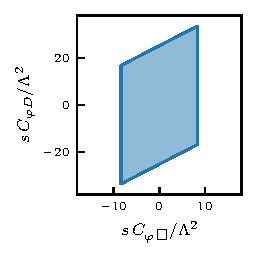
\includegraphics[scale=1.25]{images/C_H4D2.pdf}\quad
%     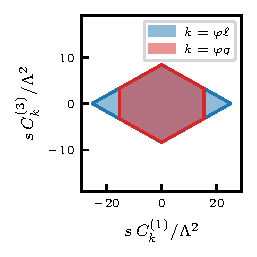
\includegraphics[scale=1.25]{images/C_Hl_and_C_Hq.pdf}\\
%     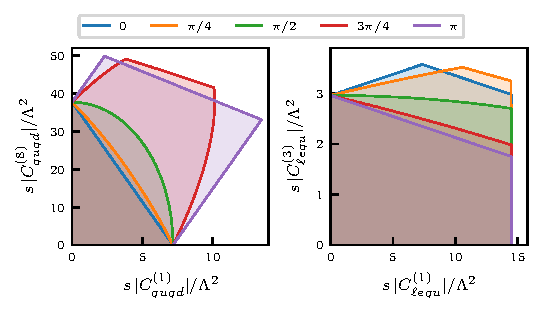
\includegraphics[scale=1.25]{images/C_quqd_and_C_lequ.pdf}
%     \caption{Parameter space allowed by unitarity bounds in the plane of Wilson coefficients in the single-flavor limit.
%     In the two lower plots, we also show the dependence on the relative complex phases $\operatorname{arg}(C_{quqd}^{(1)}/C_{quqd}^{(8)})$ and $\operatorname{arg}(C_{\ell equ}^{(1)}/C_{\ell equ}^{(3)})$.}
%     \label{fig:uni3}
% \end{figure}
\begin{figure}[htbp]
    \centering
    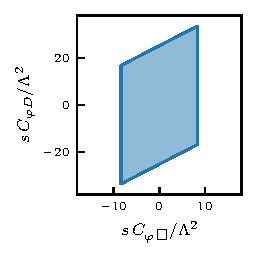
\includegraphics[width=0.25\textwidth]{images/C_H4D2.pdf}\hfill
    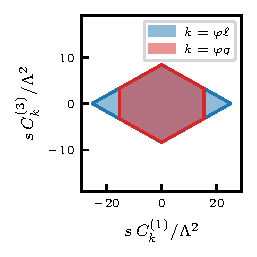
\includegraphics[width=0.25\textwidth]{images/C_Hl_and_C_Hq.pdf}\hfill
    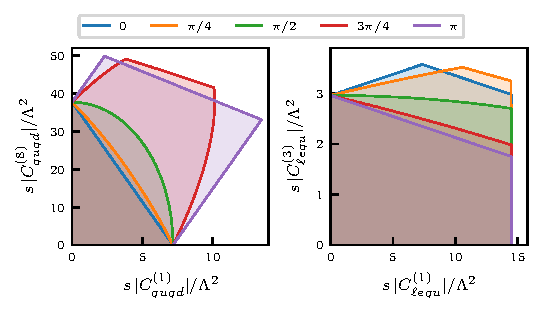
\includegraphics[width=0.48\textwidth]{images/C_quqd_and_C_lequ.pdf}
    \caption{Parameter space allowed by unitarity bounds in the plane of Wilson coefficients in the single-flavor limit.
    In the right-hand panel, we also show the dependence on the relative complex phases $\operatorname{arg}(C_{quqd}^{(1)}/C_{quqd}^{(8)})$ and $\operatorname{arg}(C_{\ell equ}^{(1)}/C_{\ell equ}^{(3)})$.}
    \label{fig:uni3}
\end{figure}

% \begin{figure}[htbp]
%     \centering
%     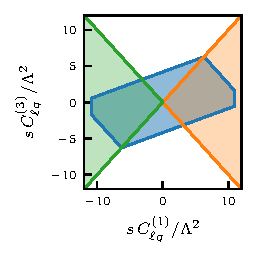
\includegraphics[scale=1.25]{images/C_lq.pdf}\qquad
%     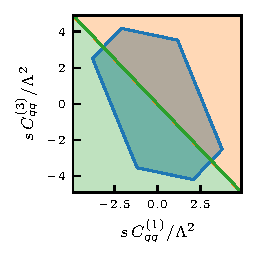
\includegraphics[scale=1.25]{images/C_qq.pdf}\\
%     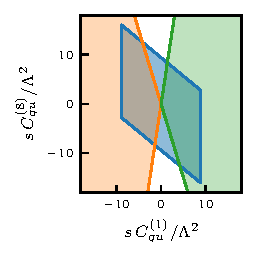
\includegraphics[scale=1.25]{images/C_qu.pdf}\qquad
%     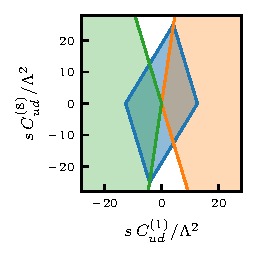
\includegraphics[scale=1.25]{images/C_ud.pdf}
%     \caption{Parameter space allowed by unitarity bounds (blue) and spinning sum rules, discussed in Section~\ref{sec:SMEFT_sumrules}, in the cases of scalar (orange) and vector (green) dominance, 
%     in the single-flavor limit. The missing plot for the Wilson coefficients $C_{qd}^{(1,8)}$ is identical to that of $C_{qu}^{(1,8)}$.}
%     \label{fig:1-flavor unitary+sum rules}
% \end{figure}
\begin{figure}[htbp]
    \centering
    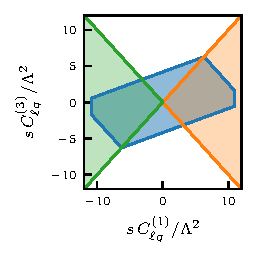
\includegraphics[width=0.25\textwidth]{images/C_lq.pdf}\hfill
    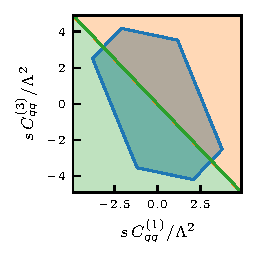
\includegraphics[width=0.25\textwidth]{images/C_qq.pdf}\hfill
    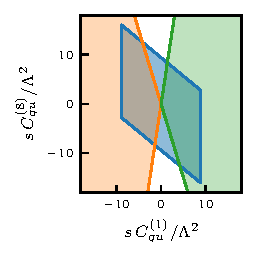
\includegraphics[width=0.25\textwidth]{images/C_qu.pdf}\hfill
    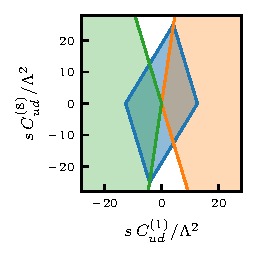
\includegraphics[width=0.25\textwidth]{images/C_ud.pdf}
    \caption{Parameter space allowed by unitarity bounds (blue) and spinning sum rules, discussed in Section~\ref{sec:SMEFT_sumrules}, in the cases of scalar (orange) and vector (green) dominance, 
    in the single-flavor limit. The missing plot for the Wilson coefficients $C_{qd}^{(1,8)}$ is identical to that of $C_{qu}^{(1,8)}$.}
    \label{fig:1-flavor unitary+sum rules}
\end{figure}

To fully exploit the power of this method, we performed a fully coupled-channel analysis
%for each operator. In particular, to compute the amplitude of a process mediated by a given SMEFT operator, we 
%considered all possible initial and final states in all allowed helicity, gauge, and flavor configurations.
by considering all possible initial and final states in all allowed helicity, gauge, and flavor configurations.
At dimension six, the leading numerical constraints often arise from the lowest-multiplicity channels. Nevertheless, the general $N \to M$ formalism of Chapter~\ref{ch:generalizedUB} is essential for a uniform treatment of all operator classes, including $\varphi^6$ and $\psi^2\varphi^3$, and makes the inclusion of higher-multiplicity channels automatic
whenever they yield the leading energy growth.
For practical purposes, we present in Table~\ref{tab:UniBounds} the unitarity bounds assuming single-flavor fermions, due to the large number of independent components arising from Wilson coefficients with multiple flavor indices.
The multi-flavor scenario is considered in Section~\ref{sec:SMEFT_multiflavor}.

The coupled-channel analysis also requires care in the choice of the angular momentum at which the
bound is imposed. 
% For operators containing a single fermionic bilinear, the lowest allowed angular
% momentum in $2\to2$ processes is $J=1/2$, reached through the channels
% \begin{gather}
%     \psi_R^{\alpha,p}\varphi_j\to \psi_L^{i,\beta,r}X^I\,,\qquad \psi_R^{\alpha,p}X^I\to \psi_L^{i,\beta,r}\varphi_j^\dagger\,,\\
%     \psi_R^{\alpha,p}\varphi_i\to\psi_R^{\beta,r}\varphi_j\,,\qquad    \psi_L^{k,\alpha,p}\varphi_i\to\psi_L^{\ell,\beta,r}\varphi_j\,,
% \end{gather}
% where $\alpha,\beta$ are $SU(3)_c$ indices in the (anti)fundamental representation and $L,R$ denote
% the chirality of the fermion fields, while at $J=1$ the additional channels are
% \begin{equation}
%     \psi_R^{\alpha,p}\overline \psi_L^{i,\beta,r}\to X^I\varphi_j^\dagger\,,\qquad \psi_R^{\alpha,p}\overline \psi_R^{\beta,r}\to\varphi_i\varphi_j^\dagger\,, \qquad \psi_L^{k,\alpha,p}\overline \psi_L^{\ell,\beta,r}\to\varphi_i\varphi_j^\dagger\,.
% \end{equation}
Operators containing a single fermionic bilinear generate $2\to2$ processes with
two fermionic and two bosonic external legs. Since a pair of fermions carries integer total angular
momentum, half-integer values of $J$ are reached only when one fermion sits in the initial and one in
the final state, and the lowest allowed value is then $J=1/2$. A minimal set of such channels is
\begin{gather}
    \psi_R^{a,p}\,\varphi^{b} \to \psi_R^{c,r}\,\varphi^{d}\,,\qquad
    \psi_L^{a,p}\,\varphi^{b} \to \psi_L^{c,r}\,\varphi^{d}\,,\qquad
    \psi_R^{a,p}\,\varphi^{b} \to \psi_L^{c,r}\,X^{d}\,,
\end{gather}
where $a,b,c,d$ collectively denote the gauge indices of each field, $p,r$ are flavor
indices, and $L,R$ denote the chirality of the fermions. The first two channels arise from the
chirality-preserving bilinears of the class $\psi^2\varphi^2D$, the third from the
chirality-violating ones of the class $\psi^2X\varphi$. All the remaining $J=1/2$ channels, such as
$\psi_R^{a,p}X^{b}\to\psi_L^{c,r}\varphi^{\dagger d}$, follow from these by applying C, P, T, or
combinations thereof.
Integer values of $J$ instead require both fermions on the same side. For $J=1$, a
minimal set of channels is
\begin{gather}
    \psi_R^{a,p}\,\overline\psi_R^{b,r} \to \varphi^{c}\,\varphi^{\dagger d}\,,\qquad
    \psi_L^{a,p}\,\overline\psi_L^{b,r} \to \varphi^{c}\,\varphi^{\dagger d}\,,\qquad
    \psi_R^{a,p}\,\overline\psi_L^{b,r} \to X^{c}\,\varphi^{\dagger d}\,,
\end{gather}
% where in the first two the chirality-preserving fermion pair already carries one unit of angular
% momentum along the collision axis, while in the third the chirality-violating pair carries none and
% the bound comes instead from the vector in the final state. 
where the minimum $J$ of each pair is set by its helicity difference, which is one unit for
the first two initial states and, in the third, for the final state.
Again, all the remaining channels follow
by applying C, P, T, or combinations thereof.
The resulting bounds are compared in Table~\ref{tab: UB for psi^2 Xphi and psi^2phi^2D}. For
operators of type $\psi^2X\varphi$ the $J=1/2$ bounds are always the stronger ones, whereas for
operators of type $\psi^2\varphi^2D$ the outcome depends on the case at hand, since in the
coupled-channel analysis the color degrees of freedom can add up and make the $J=1$ bound stronger,
even though it would naively be expected to be suppressed.

\begin{table}[tb]
\renewcommand{\arraystretch}{1.4}
\centering
\begin{tabular}{c|cc||c|cc}
\toprule
\rowcolor{hdrcolor}
\boldmath$\psi^2X\varphi$ & \boldmath$J=1/2$ & \boldmath$J=1$
& \boldmath$\psi^2\varphi^2D$ & \boldmath$J=1/2$ & \boldmath$J=1$ \\
\midrule
$C_{eW}$ & $4\pi\sqrt{2/3}$ & $4\pi\sqrt{3}$ 
& $C_{\varphi e}$ & $8\pi$ & $12\pi$ \\
$C_{eB}$ & $4\pi$ & $12\pi$ 
& $C_{\varphi u}$ & $8\pi$ & $4\pi\sqrt{3}$ \\
$C_{uW}$ & $4\pi\sqrt{2/3}$ & $4\pi$ 
& $C_{\varphi d}$ & $8\pi$ & $4\pi\sqrt{3}$ \\
$C_{dW}$ & $4\pi\sqrt{2/3}$ & $4\pi$ 
& $C_{\varphi ud}$ & $8\pi$ & $4\pi\sqrt{6}$ \\
$C_{uB}$ & $4\pi$ & $4\pi\sqrt{3}$ 
& $C_{\varphi \ell}^{(1)}$ & $8\pi$ & $6\pi\sqrt{2}$ \\
$C_{dB}$ & $4\pi$ & $4\pi\sqrt{3}$ 
& $C_{\varphi \ell}^{(3)}$ & $8\pi/3$ & $6\pi\sqrt{2}$ \\
$C_{uG}$ & $2\pi\sqrt{3}$ & $12\pi\sqrt{2}$ 
& $C_{\varphi q}^{(1)}$ & $8\pi$ & $2\pi\sqrt{6}$ \\
$C_{dG}$ & $2\pi\sqrt{3}$ & $12\pi\sqrt{2}$ 
& $C_{\varphi q}^{(3)}$ & $8\pi/3$ & $2\pi\sqrt{6}$ \\
\bottomrule
\end{tabular}
\caption{Comparison of the unitarity bounds on the modulus of the individual Wilson coefficients
associated with the operator classes $\psi^2 X \varphi$ and $\psi^2 \varphi^2 D$, resulting from the
partial waves with $J=1/2$ and $J=1$. The factors $s/\Lambda^2$ are left implicit, as in
Table~\ref{tab:UniBounds}.}
\label{tab: UB for psi^2 Xphi and psi^2phi^2D}
\end{table}


% For four-fermion operators the relevant angular momentum depends strongly on the chirality of the
% external fermions. The channels contributing at $J=0$ are
% \begin{gather}
%     \psi_R^{\alpha,p}\psi_R^{\beta,r}\to\psi_R^{\gamma,s}\psi_R^{\delta,t}\,,\qquad \psi_L^{i,\alpha,p}\psi_L^{j,\beta,r}\to\psi_L^{k,\gamma,s}\psi_L^{\ell,\delta,t}\,,\\
%     \psi_R^{\alpha,p}\psi_R^{\beta,r}\to\psi_L^{i,\gamma,s}\psi_L^{j,\delta,t}\,,\qquad \psi_R^{\alpha,p}\overline\psi_L^{i,\beta,r}\to\psi_R^{\gamma,s}\overline\psi_L^{j,\delta,t}\,,
% \end{gather}
% while those contributing at $J=1$ are
% \begin{gather}
%     \psi_R^{\alpha,p}\overline\psi_R^{\beta,r}\to\psi_R^{\gamma,s}\overline\psi_R^{\delta,t}\,,\qquad \psi_L^{i,\alpha,p}\overline\psi_L^{j,\beta,r}\to\psi_L^{k,\gamma,s}\overline\psi_L^{\ell,\delta,t}\,,\\
%     \psi_R^{\alpha,p}\overline\psi_R^{\beta,r}\to\psi_L^{i,\gamma,s}\overline\psi_L^{j,\delta,t}\,,\qquad \psi_R^{\alpha,p}\psi_L^{i,\beta,r}\to\psi_R^{\gamma,s}\psi_L^{j,\delta,t}\,.
% \end{gather}
For four-fermion operators, the relevant angular momentum is again fixed by the chirality of the
external fermions. A minimal set of channels contributing at $J=0$ is
\begin{gather}
    \psi_R^{a,p}\psi_R^{b,r}\to\psi_R^{c,s}\psi_R^{d,t}\,,\qquad
    \psi_R^{a,p}\psi_R^{b,r}\to\psi_L^{c,s}\psi_L^{d,t}\,,\qquad
    \psi_R^{a,p}\overline\psi_L^{b,r}\to\psi_R^{c,s}\overline\psi_L^{d,t}\,,
\end{gather}
while at $J=1$ it is
\begin{gather}
    \psi_R^{a,p}\overline\psi_R^{b,r}\to\psi_R^{c,s}\overline\psi_R^{d,t}\,,\qquad
    \psi_R^{a,p}\overline\psi_R^{b,r}\to\psi_L^{c,s}\overline\psi_L^{d,t}\,,\qquad
    \psi_R^{a,p}\psi_L^{b,r}\to\psi_R^{c,s}\psi_L^{d,t}\,.
\end{gather}
All the remaining channels follow by applying C, P, T, or
combinations thereof.
The corresponding bounds are compared in Table~\ref{tab: UB for psi^4}. In most cases, the $J=0$ bound
dominates, but not always, which stresses once again that, to obtain the most stringent bounds, one cannot stop at the smallest allowed
angular momentum whenever several degrees of freedom contribute to the coupled-channel analysis.

\begin{table}[htbp]
\renewcommand{\arraystretch}{1.4}
\centering
\begin{tabular}{c|cc||c|cc}
\toprule
\rowcolor{hdrcolor}
\boldmath$(\overline L L)(\overline L L)$ & \boldmath$J=0$ & \boldmath$J=1$
& {\boldmath$(\overline{L}R)(\overline{R}L)$}/{\boldmath$(\overline{L}R)(\overline{L}R)$} & \boldmath$J=0$ & \boldmath$J=1$ \\
\midrule
$C_{\ell\ell}$ & $2\pi$ & $2\pi$ 
& $C_{\ell e d q}$ & $8\pi/\sqrt{3}$ & $24\pi$ \\
$C_{qq}^{(1)}$ & $2\pi$ & $6\pi/7$ 
& $C_{quqd}^{(1)}$ & $16\pi/7$ & $24\pi$ \\
$C_{qq}^{(3)}$ & $2\pi$ & $6\pi/5$ 
& $C_{quqd}^{(8)}$ & $12\pi$ & $36\pi$ \\
$C_{\ell q}^{(1)}$ & $4\pi$ & $2\pi\sqrt{3}$ 
& $C_{\ell equ}^{(1)}$ & $8\pi/\sqrt{3}$ & $24\pi\sqrt{2}$ \\
$C_{\ell q}^{(3)}$ & $4\pi/3$ & $2\pi\sqrt{3}$ 
& $C_{\ell e qu}^{(3)}$ & $2\pi\sqrt{2}/3$ & $2\pi\sqrt{3}$ \\
\midrule
\rowcolor{hdrcolor}
\boldmath$(\overline RR)(\overline RR)$ & \boldmath$J=0$ & \boldmath$J=1$
& \boldmath$(\overline L L)(\overline R R)$ & \boldmath$J=0$ & \boldmath$J=1$ \\
\midrule
$C_{ee}$ & $2\pi$ & $3\pi$ 
& $C_{\ell e}$ & $4\pi$ & $6\pi\sqrt{2}$ \\
$C_{uu}$ & $2\pi$ & $3\pi/2$ 
& $C_{\ell u}$ & $4\pi$ & $2\pi\sqrt{6}$ \\
$C_{dd}$ & $2\pi$ & $3\pi/2$ 
& $C_{\ell d}$ & $4\pi$ & $2\pi\sqrt{6}$ \\
$C_{eu}$ & $4\pi$ & $4\pi\sqrt{3}$ 
& $C_{qe}$ & $4\pi$ & $2\pi\sqrt{6}$ \\
$C_{ed}$ & $4\pi$ & $4\pi\sqrt{3}$ 
& $C_{qu}^{(1)}$ & $4\pi$ & $2\pi\sqrt{2}$ \\
$C_{ud}^{(1)}$ & $4\pi$ & $4\pi$ 
& $C_{qu}^{(8)}$ & $3\pi$ & $12\pi\sqrt{2}$ \\
$C_{ud}^{(8)}$ & $6\pi$ & $9\pi$ 
& $C_{qd}^{(1)}$ & $4\pi$ & $2\pi\sqrt{2}$ \\
& & & $C_{qd}^{(8)}$ & $3\pi$ & $12\pi\sqrt{2}$ \\
\bottomrule
\end{tabular}
\caption{Comparison of the unitarity bounds on the modulus of the individual Wilson coefficients
associated with the four-fermion operators, resulting from the partial waves with $J=0$ and $J=1$.
The factors $s/\Lambda^2$ are left implicit, as in Table~\ref{tab:UniBounds}.}
\label{tab: UB for psi^4}
\end{table}


Lastly, for operators of the type $X^3$ involving three gauge field strengths, the unitarity bounds were computed using amplitudes that include both the SM contribution and at most one SMEFT insertion, effectively truncating the calculation at $\mathcal{O}(1/\Lambda^2)$ at the amplitude level. 
Contributions of order $1/\Lambda^4$ could, in principle, yield stronger bounds, especially when the gauge coupling is small; however, including them without simultaneously accounting for dimension-eight operators would be inconsistent.
Indeed, from positivity constraints, the presence of a dimension-six operator of type $X^3$ necessarily implies the existence of a dimension-eight operator of type $X^4$, which would inevitably affect the resulting unitarity bounds; see Ref.~\cite{Ghosh:2022qqq}.

Comparing the results in Table \ref{tab:UniBounds} with previous SMEFT analyses \cite{Corbett:2014ora,Corbett:2017qgl,Cao:2023qks}, we derive unitarity bounds for the complete set of four-fermion operators and for operators involving at least one gluon field, which were not covered in those works.
With this method, such bounds are straightforward to obtain compared to alternative approaches. Moreover, the fully exploited coupled-channel analysis allows us to derive stronger bounds than those previously reported. 

Overall, our bounds on purely bosonic operators agree with those in Ref.~\cite{Cao:2023qks}, except for a factor-of-two difference arising from Eq.~\eqref{unitarity bound general}, as that work conventionally imposed $|a_{i\to f}^J|\leq 2$ for the partial-wave coefficients. In contrast, the bounds on operators involving fermions exhibit larger discrepancies, which we attribute to the combined effects of the coupled-channel analysis and the marginalization procedure. In particular, operators of the type $\psi^2 X\varphi$ and $\psi^2\varphi^2 D$ show case-by-case differences of up to a factor of two. Overall, our bounds are always more stringent, except for $O_{\varphi ud}$, for which our bound is weaker by a factor of $\sqrt{2}$.

\section{Spinning Sum-Rule Bounds\label{sec:SMEFT_sumrules}}

As anticipated in the introduction, the analyticity of the $S$-matrix, together with partial-wave
unitarity, yields additional constraints on effective four-fermion interactions. The relevant
dispersion relations have been introduced in
Refs.~\cite{Low:2009di,Azatov:2021ygj,Gu:2020thj,Remmen:2020uze,Remmen:2022orj,Altmannshofer:2023bfk,%
Altmannshofer:2025lun}, and we derive here the resulting inequalities in the Warsaw basis.

% Following Ref.~\cite{Remmen:2020uze}, we consider the amplitude $\mathcal{A}_{\alpha\beta}(s,t)$,
% where $s$ and $t$ are the usual Mandelstam variables associated with an elastic scattering process of
% two fermions whose quantum numbers, such as flavor and helicity, are collectively denoted by $\alpha$
% and $\beta$. Expanding the UV amplitude in partial waves of fixed total angular momentum,
% $a_{\alpha\beta}^{J}(s)$, one finds\footnote{Note that our partial-wave coefficients are normalized
% differently from those of Ref.~\cite{Remmen:2020uze}.}
Following Ref.~\cite{Remmen:2020uze}, we consider the amplitude $\mathcal{A}_{\alpha\beta}(s,t)$,
where $s$ and $t$ are the usual Mandelstam variables associated with the elastic scattering of two
fermions of opposite helicity, whose internal quantum numbers, such as flavor and gauge charges, are
collectively denoted by $\alpha$ and $\beta$. We write $\overline\alpha$ for the state obtained by
crossing, with conjugated quantum numbers and reversed helicity. The initial state then carries one
unit of net helicity, so that its partial-wave expansion starts at $J=1$, whereas the crossed one has
vanishing net helicity and starts at $J=0$. Expanding the UV amplitude in partial waves of fixed
total angular momentum, $a_{\alpha\beta}^{J}(s)$, one finds\footnote{Note that our partial-wave coefficients are normalized
differently from those of Ref.~\cite{Remmen:2020uze}.}
\begin{multline}\label{eq: sum rules with boundary}
        \lim_{s\to 0}\partial_s\mathcal{A}_{\alpha\beta}(s,0)+C_{\alpha\beta}^{(s,\infty)}=-\lim_{s\to 0}\partial_s\mathcal{A}_{\overline \alpha\beta}(s,0)-C_{\overline\alpha\beta}^{(s,\infty)} \\
        =8\int_{s_0}^\infty \frac{\dd s}{s^2}\left[-\Im a_{\overline{\alpha}\beta}^{0}(s)+\sum_{J=1}^\infty(2J+1)\left(\Im a_{\alpha\beta}^{J}(s)-\Im a_{\overline{\alpha}\beta}^{J}(s)\right)\right]\,,
\end{multline}
where $s_0$ is the characteristic mass-squared scale of the UV completion and the boundary term is
defined as
\begin{equation}
    C_{\alpha\beta}^{(s,\infty)}=\Res_{s=\infty}\frac{\mathcal{A}_{\alpha\beta}(s,0)}{s^2}=-\lim_{\abs{s}\to \infty}\frac{\mathcal{A}_{\alpha\beta}(s,0)}{s}\,.
\end{equation}
The same contour argument applied to the coefficient of $t$ in $\mathcal{A}_{\alpha\beta}(0,t)$
yields a second, beyond-forward dispersion relation, with its own boundary term
$C^{(t,\infty)}_{\alpha\beta}$. Since the dimension-six amplitude of two opposite-helicity fermions
is proportional to $[13]\langle 24\rangle$, the sum of the two relations has a vanishing left-hand
side up to boundary terms, while on the right-hand side every partial wave enters with a
non-negative weight. If all boundary terms vanish and the partial-wave expansion converges, each
contribution must then vanish separately, so that $\Im a_{\alpha\beta}^{J}$ and
$\Im a_{\overline\alpha\beta}^{J}$ vanish for every $J\geq2$, together with
$\Im a_{\overline\alpha\beta}^{1}$. Only a scalar and a vector channel are left, and
Eq.~\eqref{eq: sum rules with boundary} reduces to~\cite{Remmen:2020uze}
\begin{equation}\label{eq: sum rules master equation}
    \lim_{s\to 0}\partial_s\mathcal{A}_{\overline \alpha\beta}(s,0) = -\lim_{s\to 0}\partial_s\mathcal{A}_{ \alpha\beta}(s,0) =8\int_{s_0}^\infty \frac{\dd s}{s^2}\left(\Im a_{\overline{\alpha}\beta}^{0}(s)-3\Im a_{\alpha\beta}^{1}(s)\right)\,.
\end{equation}
Dominance of spin-0 (spin-1) states in the UV theory implies that the left-hand side of
Eq.~\eqref{eq: sum rules master equation} is positive (negative) definite for any choice of $\alpha$
and $\beta$. This property can be exploited to derive constraints among the flavor-dependent entries
of the Wilson coefficients of four-fermion SMEFT operators, or between different $\psi^4$ operators
with the same fermionic content. Since Ref.~\cite{Remmen:2020uze} adopts a basis different from the
Warsaw one, we report the corresponding combinations in Table~\ref{tab:sum_rules}. When contracted
with $\alpha_p \alpha_r^* \beta^*_s \beta_t$, they are positive (negative) if the completion is
dominated by scalars (vectors).
%
\begin{table}[h!t!b!]
\renewcommand{\arraystretch}{1.5}
    \centering
    \begin{tabular}{cc}
    \toprule
    \rowcolor{hdrcolor}
    \textbf{Operator class} & \textbf{Spinning sum rules} \\
    \midrule
    \multirow{6}{*}{\boldmath$(\overline{R}R)(\overline{R}R)$} &
    $[C_{ee}]_{prst}$ \\
    & $[C_{uu}]_{prst}$\,, \qquad $[C_{uu}]_{prst} + [C_{uu}]_{ptsr}$ \\
    & $[C_{dd}]_{prst}$\,, \qquad $[C_{dd}]_{prst} + [C_{dd}]_{ptsr}$ \\
    & $[C_{eu}]_{prst}$\,, \qquad $[C_{ed}]_{prst}$ \\
    & $[C_{ud}^{(1)}]_{prst}+\tfrac{1}{4}[C_{ud}^{(8)}]_{prst}$ \\
    & $[C_{ud}^{(1)}]_{prst}-\tfrac{1}{6}[C_{ud}^{(8)}]_{prst}$ \\
    \midrule
    \multirow{5}{*}{\boldmath$(\overline{L}L)(\overline{L}L)$} &
    $[C_{\ell\ell}]_{prst}$\,, \qquad $[C_{\ell\ell}]_{prst} + [C_{\ell\ell}]_{ptsr}$ \\
    & $[C_{qq}^{(1)}]_{prst} + [C_{qq}^{(1)}]_{ptsr} + [C_{qq}^{(3)}]_{prst} + [C_{qq}^{(3)}]_{ptsr}$ \\
    & $[C_{qq}^{(1)}]_{prst} - [C_{qq}^{(3)}]_{prst} + 2[C_{qq}^{(3)}]_{ptsr}$ \\
    & $[C_{\ell q}^{(1)}]_{prst} + [C_{\ell q}^{(3)}]_{prst}$ \\
    & $[C_{\ell q}^{(1)}]_{prst} - [C_{\ell q}^{(3)}]_{prst}$ \\
    \midrule
    \multirow{6}{*}{\boldmath$(\overline{L}L)(\overline{R}R)$} &
    $-[C_{\ell e}]_{prst}$\,, \qquad $-[C_{\ell u}]_{prst}$ \\
    & $-[C_{\ell d}]_{prst}$\,, \qquad $-[C_{qe}]_{prst}$ \\
    & $-[C_{qu}^{(1)}]_{prst} - \tfrac{1}{4}[C_{qu}^{(8)}]_{prst}$ \\
    & $-[C_{qu}^{(1)}]_{prst} + \tfrac{1}{6}[C_{qu}^{(8)}]_{prst}$ \\
    & $-[C_{qd}^{(1)}]_{prst} - \tfrac{1}{4}[C_{qd}^{(8)}]_{prst}$ \\
    & $-[C_{qd}^{(1)}]_{prst} + \tfrac{1}{6}[C_{qd}^{(8)}]_{prst}$ \\
    \bottomrule
    \end{tabular}
    \caption{Combinations of four-fermion Wilson coefficients that, when contracted with $\alpha_p \alpha_r^* \beta^*_s \beta_t$, are positive (negative) if the UV completion is dominated by scalars (vectors).}
    \label{tab:sum_rules}
\end{table}
%

% Sum rules can in principle be derived for all dimension-six SMEFT Wilson coefficients. They depend,
% however, on the superposition of field states encoded in the vectors $\alpha$ and $\beta$, so that,
% even when the boundary terms vanish, they do not translate into a definite sign of the Wilson
% coefficients, unlike what happens for $\psi^4$ operators.
% For purely bosonic operators the boundary
% terms are generically present and depend on the $SU(2)_L$ configuration, so that no robust
% information can be extracted. For $\psi^2\varphi^2D$ operators one has to fix a configuration for the
% Higgs fields, after which no information is left for the flavor indices, since no spinning sum rules
% arise there~\cite{Remmen:2022orj}.

Spinning sum rules are not confined to four-fermion operators, but only for the latter do they
translate into a definite sign of a Wilson coefficient. For the purely bosonic operators of the class
$\varphi^4 D^2$, they can still be constructed, although only for a restricted cone of combinations of the
corresponding coefficients, and with the correlation between sign and spin reversed with respect to
the fermionic case~\cite{Remmen:2022orj}. For operators involving gauge bosons, the boundary terms are
generically present and depend on the $SU(2)_L$ configuration, so that the sum rules are of
indefinite sign. What survives is the sharper statement that, if the boundary terms vanish, the UV
amplitudes mediating elastic vector scattering must vanish identically~\cite{Remmen:2022orj}. For
$\psi^2\varphi^2D$ operators, one has to fix a configuration for the Higgs fields, and no spinning sum
rule arises. The dispersion relations remain informative --- vanishing boundary terms force the UV to
be dominated by a fermionic mode --- but they no longer discriminate between scalar and vector
dominance~\cite{Remmen:2022orj}.


As an illustration, Figure~\ref{fig:1-flavor unitary+sum rules} shows the parameter space allowed by
the unitarity bounds and by the spinning sum rules under scalar and vector dominance for four-fermion
Wilson coefficients in the single-flavor limit. Stronger bounds generally arise in the three-flavor
scenario, which is the subject of Section~\ref{sec:SMEFT_multiflavor}.

\subsection{Application}

We now describe how the sum rules associated with a given four-fermion operator are turned into
inequalities on its Wilson coefficients. For scalar dominance one has to impose
\begin{equation}
    b^\psi_{prst}\,\alpha_p \alpha_r^* \beta^*_s \beta_t\geq0\qquad \forall\,\alpha,\beta\,,
\end{equation}
where $\alpha,\beta$ are complex three-vectors in flavor space and $b_{prst}^\psi$ are the
combinations of Table~\ref{tab:sum_rules}. This is a double quadratic form in $\alpha$ and $\beta$.
We therefore first impose the inequality for every $\alpha$, which amounts to a quadratic form, by
introducing the $3\times 3$ matrices
\begin{equation}
    M^\psi_{pr}= b^\psi_{prst}\,\beta^*_s \beta_t
\end{equation}
and requiring all their eigenvalues to be non-negative for every $\beta$. Without loss of generality, we
parameterize
\begin{equation}
    \beta=
    \begin{pmatrix}
        e^{i\delta_1}\beta_1 \\ e^{i\delta_2}\beta_2 \\ \sqrt{1-\beta_1^2-\beta_2^2}
    \end{pmatrix}\,,
\end{equation}
% so that the eigenvalues of $M^\psi$ always take the form
% \begin{equation}\label{eq:eigenvalue form}
%     f(x)=a + bx - \sqrt{c^2 + dx + ex^2}\,,\qquad x=\beta_3^2\,,
% \end{equation}
and in all the cases encountered, the eigenvalues of $M^\psi$ take the form
\begin{equation}\label{eq:eigenvalue form}
    f_\pm(x)=a + bx \pm \sqrt{c^2 + dx + ex^2}\,,\qquad x=\beta_1^2+\beta^2_2\,,
\end{equation}
with $a,b,c,d,e\in\mathbb{R}$.
Requiring all eigenvalues to be positive for
every $\beta$ is therefore equivalent to requiring $f_-(x)\geq0$ for every $x\in[0,1]$.

% This last step is what makes the procedure practicable. 
Scanning numerically over $\beta$ would give
only a sampled, and therefore inconclusive, version of the constraint, whereas the positivity of $f_-$
on the unit interval can be traded for a finite set of algebraic inequalities among the coefficients
$a,b,c,d,e$, which are themselves functions of the Wilson coefficients. Explicitly, $f_-(x)\geq0$ for
every $x\in[0,1]$ if and only if
\begin{align}\label{eq:Delta}
    \Delta(a,b,c,d,e) &= 
    a \ge 0 
    \ \land \
    a+b \ge 0
    \ \land \ 
    a^2 - c^2 \ge 0
    \ \land \ 
    (a+b)^2 - c^2 -d-e \ge 0 \nonumber
    \\& \quad
    \land \
    [e - b^2 \ge 0 \ \lor\  (2ab-d)(2ab-d+2b^2-2e) \ge 0 \nonumber 
    \\& \quad
    \lor \ 4(b^2-e)(a^2-c^2)-(2ab-d)^2 \ge 0]
\end{align}
holds, as proved in Appendix~\ref{sec:appendix, logical expression}.
For vector dominance one follows the same steps, requiring instead all eigenvalues to be non-positive.

\subsection{Limitations}

Unlike the partial-wave unitarity bounds, which follow solely from the consistency of the EFT, the
spinning sum rules are considerably more model dependent and hold only under a specific set of
assumptions whose violation invalidates the corresponding
inequalities~\cite{Remmen:2020uze,Remmen:2022orj,Azatov:2021ygj,Gu:2020thj}. In particular:
\begin{itemize}
    \item They assume tree-level UV completions and can be violated at loop level~\cite{Azatov:2021ygj,Remmen:2020uze};
    \item They assume dominance by states of definite spin, so that completions involving a
    non-trivial interplay of spin-0 and spin-1 states can evade them, since the right-hand side of
    Eq.~\eqref{eq: sum rules master equation} ceases to be sign definite for arbitrary configurations
    of $\alpha$ and $\beta$;
    \item They rely on the vanishing of the boundary terms in the dispersion relation, which fails in
    particular for vector $t$-channel UV
    completions~\cite{Remmen:2020uze,Remmen:2022orj,Azatov:2021ygj}.
\end{itemize}
% The last condition is the most problematic one, since tree-level UV completions of $\psi^4$
% operators generically arise in new-physics models.
The last condition is the most restrictive one in practice, since $t$-channel vector mediators of
four-fermion operators arise generically in new-physics models.

This residual model dependence is, however, physically informative. A coefficient lying outside the
scalar- and vector-dominated regions does not exclude a UV completion but points to a more
structured one, such as a vector $t$-channel mediator, a loop-level origin, or a mixed-spin spectrum.
In Appendix~\ref{app:SMEFT_UV} we verify this picture explicitly by matching a representative set of
tree-level UV completions of Ref.~\cite{deBlas:2017xtg}. All the scalar completions considered there satisfy the
sum-rule constraints, whereas vector $t$-channel completions can violate them.

\section{Bounds on Flavorful Four-Fermion Operators\label{sec:SMEFT_multiflavor}}

The results presented so far assume a single fermion flavor. In the SMEFT, the basis of $\psi^4$
operators accounts for thousands of independent coefficients once the full flavor structure of the SM
fermions is turned on. Specific hypotheses about the symmetries and the symmetry breaking in the
flavor sector therefore play an important role in addressing the question of what information can be
extracted from the theoretical bounds derived above. The drawback is that this necessarily introduces
some model dependence. Still, reasonable flavor hypotheses have been proposed in the literature and
used in many beyond-the-SM studies, precisely in order to deal with the proliferation of independent
$\psi^4$ Wilson coefficients.

\subsection{Flavor Symmetries}

Historically, the most widely adopted hypothesis is Minimal Flavor Violation (MFV), first introduced
in Ref.~\cite{DAmbrosio:2002vsn} for the quark sector and subsequently extended to the
leptons~\cite{Cirigliano:2005ck}. It assumes that the SM fermions are charged under the global flavor
symmetry group
\begin{equation}
    G_{\rm MFV}\equiv U(3)^5=U(3)_q\times U(3)_u\times U(3)_d\times U(3)_\ell\times U(3)_e\,,
\end{equation}
where each SM fermion is a three-vector in flavor space transforming in the fundamental
representation of one of these factors,
\begin{equation}
    q\to U_q\, q\,,\quad \ell\to U_\ell\, \ell\,,\quad u\to U_u\, u\,,\quad d\to U_d\, d\,,\quad e\to U_e\, e\,.
\end{equation}
The only interactions in the SM Lagrangian that explicitly break $G_{\rm MFV}$ are the Yukawa
matrices $Y_u$, $Y_d$ and $Y_e$, which are promoted to spurions transforming as
\begin{equation}
    Y_u\to U_q Y_u U_u^\dagger\,,\quad Y_d\to U_q Y_d U_d^\dagger\,,\quad Y_e\to U_\ell Y_e U_e^\dagger\,.
\end{equation}
Assuming that new physics also respects $G_{\rm MFV}$, the number of independent coefficients in
four-fermion operators is strongly reduced, since $U(3)^5$-violating terms can arise only through
appropriate Yukawa insertions in the Wilson coefficients, weighted by unknown $\mathcal O(1)$
numbers. The classification of the independent structures arising at dimension six was carried out in
Ref.~\cite{Faroughy:2020ina}. Furthermore, since all the entries of the Yukawa matrices are nearly
vanishing except $[Y_u]_{33}\approx y_t\approx 1$, we neglect all the flavor structures involving
insertions of $Y_d$ or $Y_e$ and retain only the exact structures together with those up to
$\mathcal O(Y_u^2)$.\footnote{In principle, since $y_t\approx1$, an arbitrary number of $Y_u$
insertions should be considered, but this would amount to an effective breaking $U(3)_q\times U(3)_u\to
U(2)_q\times U(2)_u$. We stop at $\mathcal{O}(Y_u^2)$.} In this way the independent coefficients of
$\psi^4$ operators are reduced from $\mathcal O(1000)$ to $\mathcal O(10)$.

Another theoretically motivated hypothesis assumes that the first two generations of each fermion
species transform collectively as doublets while the third generation is a singlet. The flavor
symmetry is then
\begin{equation}
    G_{\rm F}\equiv U(2)^5=U(2)_q\times U(2)_u\times U(2)_d\times U(2)_\ell\times U(2)_e\,,
\end{equation}
where the fermion fields decompose as $\psi = (\psi_a,\psi_3)$, with $a=1,2$ and
$\psi=q,u,d,\ell,e$. The classification of the independent structures at dimension six was again
carried out in Ref.~\cite{Faroughy:2020ina}. In this case there is no unique or well-motivated choice
of spurions parameterizing the breaking of the symmetry~\cite{Faroughy:2020ina,Greljo:2022cah}, but
they are always expected to be small, so that we retain only the exact flavor structures. The number
of independent coefficients of $\psi^4$ operators is again reduced from $\mathcal O(1000)$ to
$\mathcal O(10)$.

In the following we make the symmetrization of the Wilson coefficients explicit, since the bounds
require computing eigenvalues of quadratic forms. For operators built from a single fermion species
we use
\begin{equation}
    [C_{\psi\psi}]_{prst}=[C_{\psi\psi}]_{stpr}=[C_{\psi\psi}]^*_{rpts}\,,
\end{equation}
while for different fermion types
\begin{equation}
    [C_{\psi\chi}]_{prst}=[C_{\psi\chi}]^*_{rpts}\,.
\end{equation}

\subsection{\texorpdfstring{Example: $O_{\ell q}^{(1)}$ and $O_{\ell q}^{(3)}$}{Example: Olq(1) and Olq(3)}}

Under these flavor hypotheses we are able to provide unitarity bounds for the SMEFT Wilson
coefficients involving fermionic fields in the multi-flavor case. As a representative example, we
discuss here the operators $O_{\ell q}^{(1,3)}$. Under MFV each of them admits two independent
coefficients,
\begin{equation}
    [C_{\ell q}^{(i)}]_{prst} = C_{\ell q}^{(i,1)}\delta_{pr}\delta_{st}
    + C_{\ell q}^{(i,2)}\delta_{pr}(Y_u Y_u^\dagger)_{st}\,,\qquad i=1,3\,,
\end{equation}
while under $U(2)^5$ the independent structures are four for each $i$. The corresponding marginalized
bounds are collected in Table~\ref{tab:Olq_UB}, and the allowed regions are shown in
Figures~\ref{fig:Olq_mfv} and \ref{fig:Olq_u2} as two-dimensional slices, in which the remaining
independent coefficients are set to zero.

\begin{table}[htbp]
\centering
{\small
% ---- info block ----
\begin{tabular}{ll}
    \textbf{Operators:} &
        $\boxed{O_{\ell q}^{(1)} = (\overline\ell_p \gamma^\mu \ell_r)(\overline q_s \gamma_\mu q_t),\quad O_{\ell q}^{(3)} = (\overline\ell_p \gamma^\mu \sigma^I \ell_r)(\overline q_s \gamma_\mu \sigma^I q_t)}$ \\[0.2cm]
    \textbf{MFV decomposition:} &
        $[C_{\ell q}^{(i)}]_{prst} =
            C_{\ell q}^{(i,1)}\delta_{pr}\delta_{st}
            + C_{\ell q}^{(i,2)}\delta_{pr}(Y_u Y_u^\dagger)_{st}$,\quad $i=1,3$ \\[0.15cm]
    \textbf{$U(2)^5$ decomposition:} &
        $[C_{\ell q}^{(i)}]_{prst} =
            C_{\ell q}^{(i,1)}\Pij{p}{r}{a}\Pij{s}{t}{b}
            + C_{\ell q}^{(i,2)}\delta_{p3}\delta_{3r}\Pij{s}{t}{a}
            $ \\
        & $\phantom{[C_{\ell q}^{(i)}]_{prst} ={}}+ C_{\ell q}^{(i,3)}\Pij{p}{r}{a}\delta_{s3}\delta_{3t}
            + C_{\ell q}^{(i,4)}\delta_{p3}\delta_{3r}\delta_{s3}\delta_{3t}$,\quad $i=1,3$ \\
\end{tabular}
\\[0.3cm]
% ---- bounds table ----
\renewcommand{\arraystretch}{1.3}
\begin{tabular}{ccccc}
    \toprule
    \rowcolor{hdrcolor}
    \textbf{Symmetry} & \textbf{Coefficient}
        & \textbf{Unitarity bound}
        & \textbf{Scalar dominance}
        & \textbf{Vector dominance} \\
    \midrule
    % --- MFV section ---
    %\rowcolor{seccolor}
    %\multicolumn{5}{l}{\textit{Minimal Flavor Violation}} \\
    \multirow{4}{*}{MFV}
        & $C_{\ell q}^{(1,1)}$ & $[-4.44,\, 4.44]$ & $[0,\, 4.44]$      & $[-4.44,\, 0]$    \\
        & $C_{\ell q}^{(1,2)}$ & $[-7.70,\, 7.70]$ & $[-4.44,\, 6.28]$  & $[-6.28,\, 4.44]$ \\
        & $C_{\ell q}^{(3,1)}$ & $[-4.44,\, 4.44]$ & $[-3.14,\, 4.44]$  & $[-4.44,\, 3.14]$ \\
        & $C_{\ell q}^{(3,2)}$ & $[-7.70,\, 7.70]$ & $[-6.99,\, 7.70]$  & $[-7.70,\, 6.99]$ \\
    \midrule
    % --- U(2)^5 section ---
    %\rowcolor{seccolor}
    %\multicolumn{5}{l}{\textit{$U(2)^5$ Flavor Symmetry}} \\
    \multirow{8}{*}{$U(2)^5$}
        & $C_{\ell q}^{(1,1)}$ & $[-5.44,\, 5.44]$ & $[0,\, 5.44]$      & $[-5.44,\, 0]$    \\
        & $C_{\ell q}^{(1,2)}$ & $[-7.70,\, 7.70]$ & $[0,\, 7.70]$      & $[-7.70,\, 0]$    \\
        & $C_{\ell q}^{(1,3)}$ & $[-7.70,\, 7.70]$ & $[0,\, 7.70]$      & $[-7.70,\, 0]$    \\
        & $C_{\ell q}^{(1,4)}$ & $[-10.9,\, 10.9]$ & $[0,\, 10.9]$      & $[-10.9,\, 0]$    \\
        & $C_{\ell q}^{(3,1)}$ & $[-5.44,\, 5.44]$ & $[-3.14,\, 5.44]$  & $[-5.44,\, 3.14]$ \\
        & $C_{\ell q}^{(3,2)}$ & $[-6.28,\, 6.28]$ & $[-3.14,\, 6.28]$  & $[-6.28,\, 3.14]$ \\
        & $C_{\ell q}^{(3,3)}$ & $[-6.28,\, 6.28]$ & $[-3.14,\, 6.28]$  & $[-6.28,\, 3.14]$ \\
        & $C_{\ell q}^{(3,4)}$ & $[-6.28,\, 6.28]$ & $[-3.14,\, 6.28]$  & $[-6.28,\, 3.14]$ \\
    \bottomrule
\end{tabular}}
\caption{Marginalized partial-wave unitarity bounds for $O_{\ell q}^{(1,3)}$ under MFV and $U(2)^5$
flavor symmetry, with and without spinning sum rules under scalar or vector dominance in the UV.
Bounds are intervals $[a,b]$ with $(s/\Lambda^2)C \in [a,b]$, rounded to 3 significant digits.}
\label{tab:Olq_UB}
\end{table}


\begin{figure}[htbp]
    \centering
    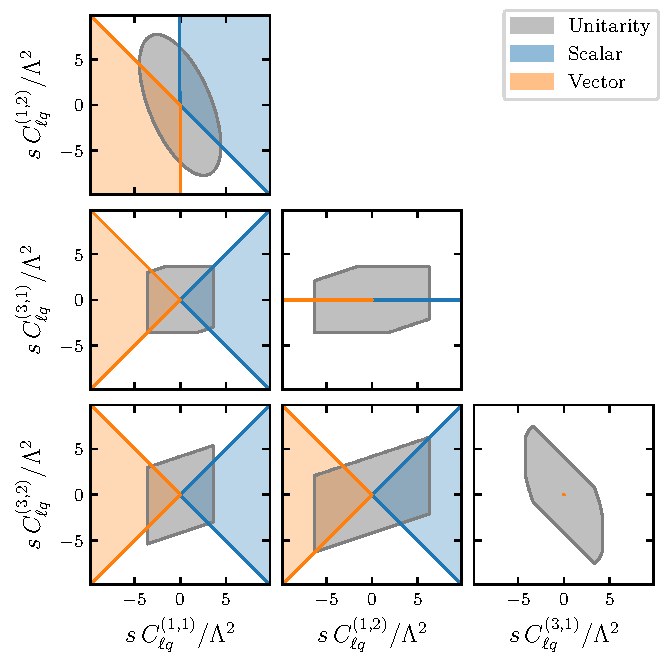
\includegraphics[scale = 0.75]{images/flavor/Olq_mfv.pdf}
    \caption{Partial-wave unitarity bounds and sum-rule constraints (under scalar and vector dominance) for the operators $O_{\ell q}^{(1,3)}$ under MFV, where $[C_{\ell q}^{(i)}]_{prst} =
            C_{\ell q}^{(i,1)}\delta_{pr}\delta_{st}
            + C_{\ell q}^{(i,2)}\delta_{pr}(Y_u Y_u^\dagger)_{st}$, $i=1,3$. The regions shown are two-dimensional slices of the full allowed region, obtained by setting to zero all the independent coefficients other than the two displayed.}
    \label{fig:Olq_mfv}
\end{figure}

\begin{figure}[htbp]
    \centering
    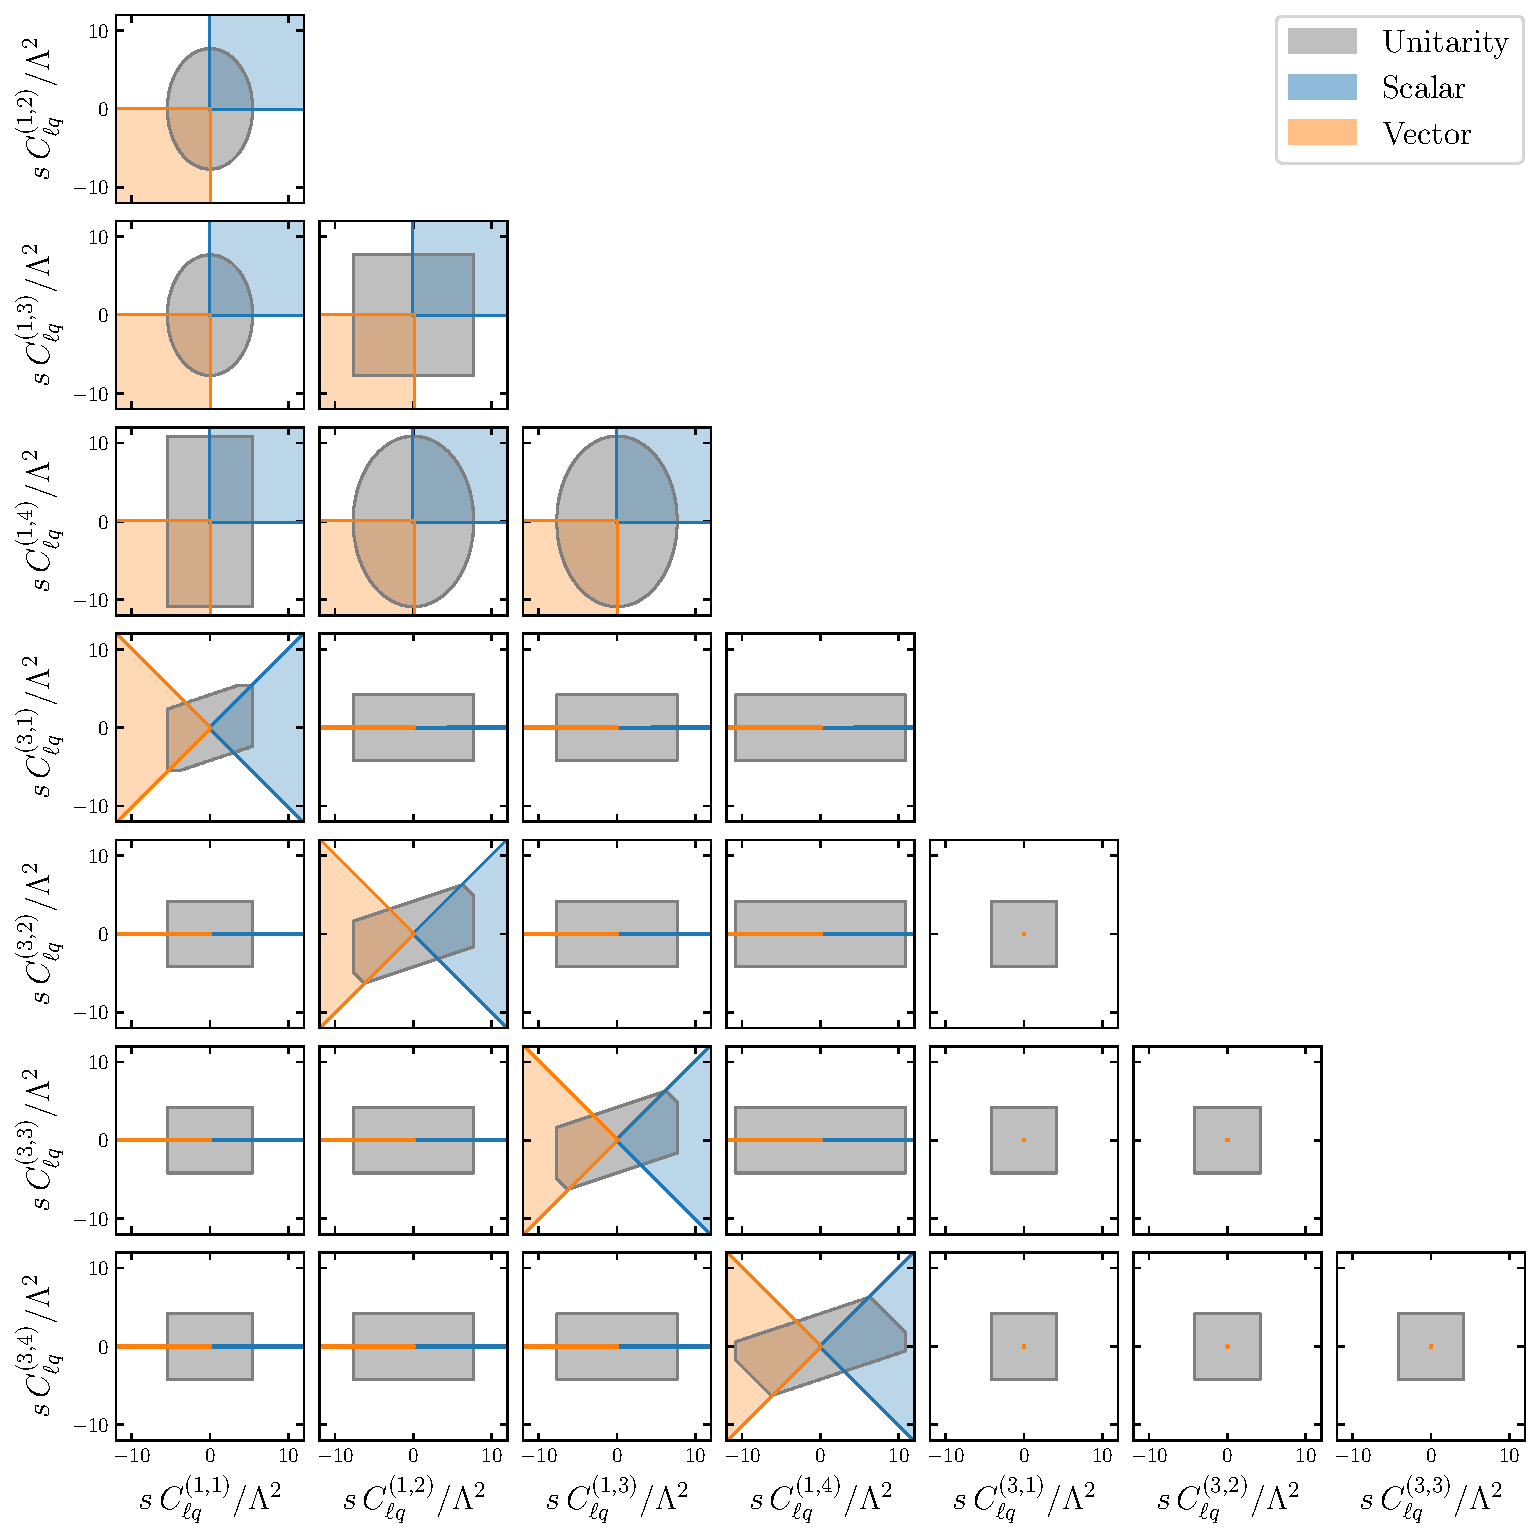
\includegraphics[width=1\linewidth]{images/flavor/Olq_u2.pdf}
    \caption{Partial-wave unitarity bounds and sum-rule constraints (under scalar and vector dominance) for the operators $O_{\ell q}^{(1,3)}$ under $U(2)^5$ flavor symmetry, where $[C_{\ell q}^{(i)}]_{prst} =
            C_{\ell q}^{(i,1)}\Pij{p}{r}{a}\Pij{s}{t}{b}
            + C_{\ell q}^{(i,2)}\delta_{p3}\delta_{3r}\Pij{s}{t}{a}
            + C_{\ell q}^{(i,3)}\Pij{p}{r}{a}\delta_{s3}\delta_{3t}
            + C_{\ell q}^{(i,4)}\delta_{p3}\delta_{3r}\delta_{s3}\delta_{3t}$, $i=1,3$. The regions shown are two-dimensional slices of the full allowed region, obtained by setting to zero all the independent coefficients other than the two displayed.}
    \label{fig:Olq_u2}
\end{figure}


Interestingly, one can notice that setting some coefficients to zero forces the other coefficients to vanish as well in order to satisfy the sum-rule constraints.
This can be seen, e.g., in two panels of Figure~\ref{fig:Olq_mfv} and eighteen panels of Figure~\ref{fig:Olq_u2}, where the sum-rule regions collapse to lines or points.

Even under these flavor hypotheses, the coupled-channel analysis remains demanding. As an illustration,
Figure~\ref{fig:matrixplot} shows the structure of the scattering matrix --- whose
eigenvalues were obtained analytically with finite-field methods~\cite{Chestnov:2025svg} --- associated with the
$q\overline q \to q \overline q$ processes in the three-flavor $U(2)^5$ scenario, considered for obtaining the bounds associated with $O_{qq}^{(1,3)}$.
%
\begin{figure}[htbp]
    \centering
    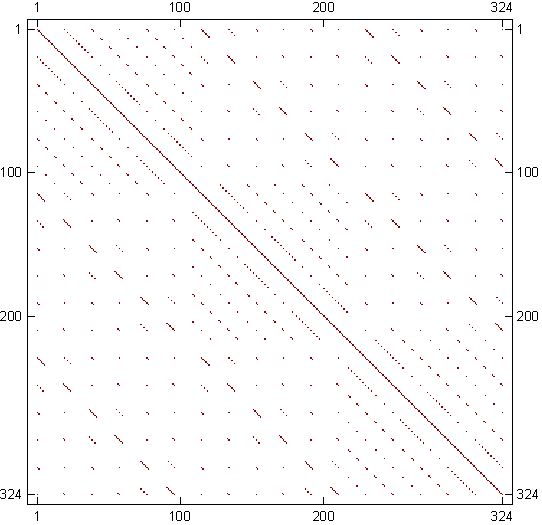
\includegraphics[scale=0.9]{images/matrixplot.pdf}
    \caption{Structure of scattering matrix associated with the $q\overline q \to q \overline q$ processes in the three-flavor scenario under the $U(2)^5$ flavor symmetry. The dimension of the matrix is $324=18^2$ as each $q$ or $\overline q$ contains $3\times 3\times 2$ degrees of freedom. To obtain its eigenvalues analytically, finite-field methods have been employed~\cite{Chestnov:2025svg}.}
    \label{fig:matrixplot}
\end{figure}

The same analysis has been carried out for all the remaining four-fermion operators. Since the
resulting set of flavor structures, bounds, and allowed regions is extensive, we collect it in
Appendix~\ref{app:SMEFT_flavorresults}.

\section{Phenomenological Applications\label{sec:SMEFT_pheno}}

To assess the phenomenological impact of the theoretical bounds discussed above, it is useful to examine their complementarity with both current and anticipated future experimental constraints.

We first analyze the unitarity bounds for purely bosonic operators. Figure~\ref{fig:histogram} shows the minimum energy scales $E_*$ at which the bounds in Table~\ref{tab:UniBounds} are violated, assuming Wilson coefficients are taken from the 95\% CL marginalized intervals of Ref.~\cite{Celada:2024mcf}, using linear (blue) and quadratic (orange) fits.
%
\begin{figure}[htbp]
    \centering
    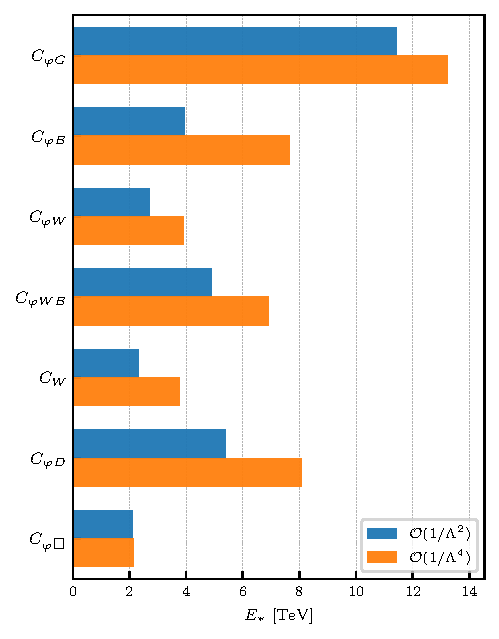
\includegraphics[scale=1.0]{images/histogram.pdf}
    \caption{Minimum energy scales $E_*$ at which the unitarity bounds in Table~\ref{tab:UniBounds} are violated for each purely bosonic Wilson coefficient in Ref.~\cite{Celada:2024mcf}, using the 95\% CL marginalized intervals from linear (blue) and quadratic (orange) fits.}
    \label{fig:histogram}
\end{figure}

Moreover, Figure~\ref{fig:3plotsa} presents both the unitarity bounds and the experimental constraints from LEP and (HL-)LHC diboson data on the Wilson coefficients of the operators $O_{\varphi q}^{(1)}$ and $O_{\varphi q}^{(3)}$.
\begin{figure}[htbp]
    \centering
    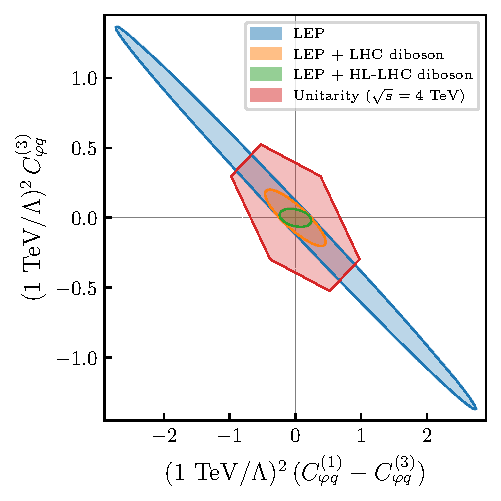
\includegraphics[scale=1]{images/dibosonv2.pdf}
    \caption{Experimental and unitarity constraints on the Wilson coefficients of the operators $O_{\varphi q}^{(1)} = \sum_{p=1,2}i(\varphi^\dagger \overset{\leftrightarrow}{D}{}_\mu \varphi)(\overline q_p \gamma^\mu q_p)$ and $O_{\varphi q}^{(3)} = \sum_{p=1,2}i(\varphi^\dagger \overset{\leftrightarrow}{D}{}_\mu^I \varphi)(\overline q_p \sigma^I \gamma^\mu q_p)$. Experimental limits correspond to $95\%$ CL marginalized intervals \cite{Celada:2024mcf}.}
    \label{fig:3plotsa}
\end{figure}
The experimental limits correspond to 95\% CL marginalized intervals obtained from a linear fit \cite{Celada:2024mcf}. As shown, the unitarity bounds --- scaling as $(\sqrt{s}/4~\mathrm{TeV})^2$ --- are significantly stronger than those from LEP alone, but remain weaker than the constraints derived from the combined LEP and (HL-)LHC data.

As a third example, we consider the global analysis of LHC Run II data in the top sector induced by the four-quark operators $O_{Qq}^{1,8}$ and $O_{Qq}^{3,8}$, where the experimental limits are obtained from a quadratic fit \cite{Brivio:2019ius}.
\begin{figure}[htbp]
    \centering
    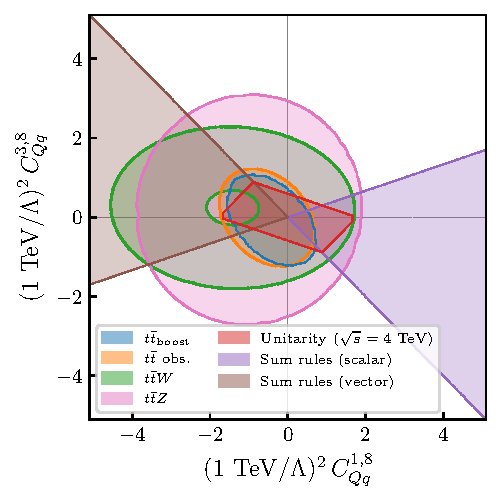
\includegraphics[scale=1]{images/top.pdf}
    \caption{Experimental and unitarity constraints on the Wilson coefficients of the 
    operators $O_{Qq}^{1,8} = \sum_{p=1,2}(\overline q_3 \gamma_\mu T^A q_3)(\overline q_p \gamma^\mu T^A q_p)$ and $O_{Qq}^{3,8} = \sum_{p=1,2}(\overline q_3 \gamma_\mu T^A \sigma^I q_3)(\overline q_p \gamma^\mu T^A \sigma^I q_p)$. 
    Experimental limits correspond to $68\%$ CL and are derived from a quadratic fit \cite{Brivio:2019ius}. Here, the sum rules select the region where $C_{Qq}^{1,8}-(1\pm 2)C_{Qq}^{3,8}$ are positive (negative) for scalar (vector) completions.}
    \label{fig:3plotsb}
\end{figure}
Most of the measurements involve final states with a top-quark pair, including kinematic distributions, the charge asymmetry, and associated top-pair production with a weak boson. As shown in Figure~\ref{fig:3plotsb}, the unitarity bounds are quite competitive with the LHC experimental limits. Interestingly, the inclusion of sum rules --- corresponding to an underlying scalar or vector tree-level mediator of the four-fermion interactions --- selects complementary regions of the parameter space, thereby providing insight into the nature of the underlying new-physics dynamics.

As a last example, we consider the comprehensive analysis of electroweak, flavor, and collider constraints on semileptonic 
four-fermion operators $[O_{\ell q}^{(1)}]_{3333}$ and $[O_{\ell q}^{(3)}]_{3333}$ in the $U(2)^5$ scenario of Ref.~\cite{Allwicher:2023shc}, where new physics predominantly couples to the third generation. Also in this case, as shown in Figure~\ref{fig:3plotsc}, the unitarity bounds and the sum-rule constraints are highly complementary and competitive with the experimental limits.
\begin{figure}[htbp]
    \centering
    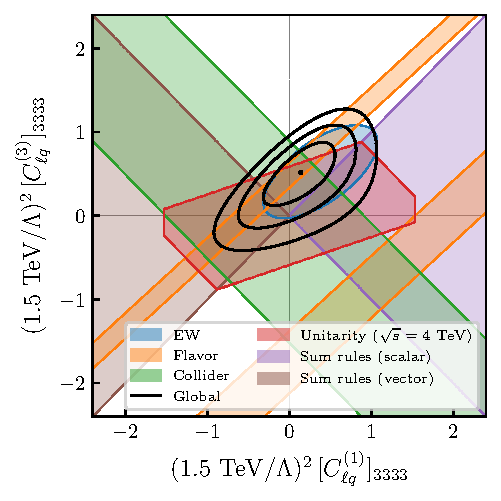
\includegraphics[scale=1]{images/flavor.pdf}
    \caption{Experimental and unitarity constraints on the Wilson coefficients of the 
    operators $[O_{\ell q}^{(1)}]_{3333} = (\overline \ell_3 \gamma^\mu \ell_3)(\overline q_3 \gamma_\mu q_3)$ and $[O_{\ell q}^{(3)}]_{3333} = (\overline \ell_3 \gamma^\mu \sigma^I \ell_3)(\overline q_3 \gamma_\mu \sigma^I q_3)$.
    Experimental limits correspond to $68\%$ CL \cite{Allwicher:2023shc}.}
    \label{fig:3plotsc}
\end{figure}
In particular, it is noteworthy that the $1\sigma$ region of the global fit lies outside the regions preferred by the sum rules. 
If the current experimental situation is confirmed and further strengthened, this would favor, for instance, an underlying $t$-channel UV completion.

These experimental contours are not recomputed by imposing an additional unitarity cut; the unitarity bounds should instead be interpreted as a theoretical consistency overlay.

As a final remark, the unitarity bounds constrain the
combination $\hat s|C|/\Lambda^2$, so that the
corresponding limits become increasingly stringent at
larger values of the partonic center-of-mass energy
$\sqrt{\hat s}$. Since perturbative unitarity determines
the range of validity of the EFT, the relevant scale
entering the bound is $\sqrt{\hat s}$, rather than the
collider center-of-mass energy itself. 

This is
particularly relevant for the HL-LHC: although it
operates at the same collider energy as the LHC, its
much larger integrated luminosity enables precision
measurements deeper into the high-energy tails of
differential distributions, thereby extending the range
of partonic scales over which the SMEFT description can
be meaningfully tested. Accordingly, while most collider
constraints discussed here probe partonic
center-of-mass energies of order
$\sqrt{\hat s}\sim 2$~TeV, we display the unitarity
bounds at $\sqrt{\hat s}=4$~TeV as a
representative benchmark for the multi-TeV regime
accessible in HL-LHC measurements. 

In realistic
analyses with a broad partonic energy spectrum, the
unitarity condition should instead be evaluated at the
value of $\sqrt{\hat s}$ relevant for each event or
kinematic bin, thereby defining the maximum hard scale
up to which the SMEFT description remains
perturbatively self-consistent.

\section{Conclusions\label{sec:SMEFT_conclusions}}

Non-renormalizable interactions induce scattering amplitudes that grow with energy, potentially
leading to violations of perturbative unitarity at high scales. A consistent interpretation of
experimental data, particularly at the High-Luminosity LHC and at future high-energy colliders,
therefore requires quantitative theoretical criteria to assess the range of validity of the SMEFT
description.

In this chapter we have performed a comprehensive reassessment of perturbative unitarity bounds on
all dimension-six SMEFT Wilson coefficients, significantly extending and sharpening the partial
results previously reported in the literature; see Table~\ref{tab:UniBounds}. The bound associated
with each Wilson coefficient was obtained by marginalizing over all the others, so that the numbers
quoted are conservative one-dimensional projections of the full coupled-channel unitarity region
rather than single-operator bounds; see Figures~\ref{fig:uni3} and
\ref{fig:1-flavor unitary+sum rules}. We performed a fully coupled-channel analysis, including all
allowed initial and final states across helicity, gauge, and flavor configurations, thereby deriving
stronger bounds than previously reported. In particular, we derived unitarity bounds for the complete
set of four-fermion operators as well as for operators involving gluon fields, which were not covered
in previous SMEFT studies~\cite{Corbett:2014ora,Corbett:2017qgl,Cao:2023qks}. The general $N\to M$
formalism of Chapter~\ref{ch:generalizedUB} was essential to treat all operator classes uniformly,
and in particular to constrain $O_\varphi$, which admits no $2\to2$ channel at all.

We then derived the spinning sum rules for four-fermion operators in the Warsaw basis and provided an operative procedure to translate them
into inequalities on the Wilson coefficients in flavor space. We also delimited their regime of
validity, identifying three distinct mechanisms through which they can fail and illustrated them with explicit UV completions.

Relaxing the single-flavor assumption, we presented the bounds on four-fermion operators under the
MFV and $U(2)^5$ flavor hypotheses, which reduce the $\mathcal O(1000)$ independent coefficients to
$\mathcal O(10)$ and make the multi-flavor analysis tractable.

As shown in Figures~\ref{fig:3plotsa}--\ref{fig:3plotsc}, these theoretical constraints are already
competitive with, and in some cases stronger than, the corresponding experimental bounds at energy
scales above a few TeV. This is particularly relevant for four-fermion operators under realistic
flavor assumptions motivated by the SM flavor puzzle, where the unitarity limits can be further
strengthened by imposing the sum rules. Interestingly, the sum rules select complementary regions of
the parameter space, thereby providing insight into the nature of the underlying new-physics
dynamics.

More broadly, the framework developed here establishes the first systematic, per\-tur\-ba\-ti\-vi\-ty-based
criterion that naturally incorporates operator correlations and can be directly implemented in
present and future global SMEFT analyses, collider phenomenology, and Monte Carlo event generation.
The results derived in this chapter strengthen the connection between theoretical and experimental
constraints in future searches for physics beyond the Standard Model.

\begin{subappendices}

\section{Conventions\label{app:SMEFT_conv}}
In Table~\ref{tab:WarsawBasis} we report the baryon-number-conserving dimension-six operators of the SMEFT in the Warsaw basis \cite{Grzadkowski:2010es}.
%
\begin{table}[tb]
\renewcommand{\arraystretch}{1.5}
    \centering
    \resizebox{\textwidth}{!}{
    \begin{tabular}{c | c|c | c|c| c|c| c|c| c}
    \toprule
    %\toprule
    \rowcolor{hdrcolor}
    \multicolumn{2}{c|}{{\boldmath$X^3$}} & \multicolumn{2}{c|}{{\boldmath$\varphi^6$}/{\boldmath$\varphi^4D^2$}} & \multicolumn{2}{c|}{{\boldmath$\psi^2\varphi^3$}} & \multicolumn{2}{c|}{{\boldmath$(\overline{L}L)(\overline{L}L)$}} & \multicolumn{2}{c}{{\boldmath$(\overline{L}R)(\overline{R}L)$}/{\boldmath$(\overline{L}R)(\overline{L}R)$}} \\
    \hline
    $O_G$ & $f^{ABC} G_\mu^{A\nu} G_\nu^{B\rho} G_\rho^{C\mu}$ & $O_\varphi$ & $(\varphi^\dagger \varphi)^3$ & $^\ddagger O_{e\varphi}$ & $(\varphi^\dagger \varphi)(\overline{\ell}_p e_r \varphi)$ & $O_{\ell\ell}$ & $(\overline{\ell}_p \gamma_\mu \ell_r)(\overline{\ell}_s \gamma^\mu \ell_t)$ & $^\ddagger O_{\ell edq}$ & $(\overline{\ell}_p^j e_r)(\overline{d}_s q_{tj})$ \\
    
    $O_{\widetilde{G}}$ & $f^{ABC} \widetilde{G}_\mu^{A\nu} G_\nu^{B\rho} G_\rho^{C\mu}$ & $O_{\varphi\Box}$ & $(\varphi^\dagger \varphi)\Box(\varphi^\dagger \varphi)$ & $^\ddagger O_{u\varphi}$ & $(\varphi^\dagger \varphi)(\overline{q}_p u_r \widetilde{\varphi})$ & $O_{qq}^{(1)}$ & $(\overline{q}_p \gamma_\mu q_r)(\overline{q}_s \gamma^\mu q_t)$ & $^\ddagger O_{quqd}^{(1)}$ & $(\overline{q}_p^j u_r)\epsilon_{jk}(\overline{q}_s^k d_t)$ \\
    
    $O_W$ & $\epsilon^{IJK} W_\mu^{I\nu} W_\nu^{J\rho} W_\rho^{K\mu}$ & $O_{\varphi D}$ & $(\varphi^\dagger D^\mu \varphi)^* (\varphi^\dagger D_\mu \varphi)$ & $^\ddagger O_{d\varphi}$ & $(\varphi^\dagger \varphi)(\overline{q}_p d_r \varphi)$ & $O_{qq}^{(3)}$ & $(\overline{q}_p \gamma_\mu \sigma^I q_r)(\overline{q}_s \gamma^\mu \sigma^I q_t)$ & $^\ddagger O_{quqd}^{(8)}$ & $(\overline{q}_p^j T^A u_r)\epsilon_{jk}(\overline{q}_s^k T^A d_t)$ \\
    
    $O_{\widetilde{W}}$ & $\epsilon^{IJK} \widetilde{W}_\mu^{I\nu} W_\nu^{J\rho} W_\rho^{K\mu}$ & & & & & $O_{\ell q}^{(1)}$ & $(\overline{\ell}_p \gamma_\mu \ell_r)(\overline{q}_s \gamma^\mu q_t)$ & $^\ddagger O_{\ell equ}^{(1)}$ & $(\overline{\ell}_p^j e_r)\epsilon_{jk}(\overline{q}_s^k u_t)$ \\
    
    & & & & & & $O_{\ell q}^{(3)}$ & $(\overline{\ell}_p \gamma_\mu \sigma^I \ell_r)(\overline{q}_s \gamma^\mu \sigma^I q_t)$ & $^\ddagger O_{\ell equ}^{(3)}$ & $(\overline{\ell}_p^j \sigma_{\mu\nu} e_r)\epsilon_{jk}(\overline{q}_s^k \sigma^{\mu\nu} u_t)$ \\
    
    \midrule
    %\midrule
    \rowcolor{hdrcolor}
    \multicolumn{2}{c|}{{\boldmath$X^2\varphi^2$}} & \multicolumn{2}{c|}{{\boldmath$\psi^2 X \varphi$}} & \multicolumn{2}{c|}{{\boldmath$\psi^2\varphi^2D$}} & \multicolumn{2}{c|}{{\boldmath$(\overline{R}R)(\overline{R}R)$}} & \multicolumn{2}{c}{{\boldmath$(\overline{L}L)(\overline{R}R)$}} \\
    \hline
    $O_{\varphi G}$ & $(\varphi^\dagger \varphi) G_{\mu\nu}^A G^{A\mu\nu}$ & $^\ddagger O_{eW}$ & $(\overline{\ell}_p \sigma^{\mu\nu} e_r)\sigma^I \varphi W_{\mu\nu}^I$ & $O_{\varphi\ell}^{(1)}$ & $(\varphi^\dagger i\overset{\leftrightarrow}{D}{}_\mu \varphi)(\overline{\ell}_p \gamma^\mu \ell_r)$ & $O_{ee}$ & $(\overline{e}_p \gamma_\mu e_r)(\overline{e}_s \gamma^\mu e_t)$ & $O_{\ell e}$ & $(\overline{\ell}_p \gamma_\mu \ell_r)(\overline{e}_s \gamma^\mu e_t)$ \\
    
    $O_{\varphi \widetilde{G}}$ & $(\varphi^\dagger \varphi) \widetilde{G}_{\mu\nu}^A G^{A\mu\nu}$ & $^\ddagger O_{eB}$ & $(\overline{\ell}_p \sigma^{\mu\nu} e_r)\varphi B_{\mu\nu}$ & $O_{\varphi\ell}^{(3)}$ & $(\varphi^\dagger i\overset{\leftrightarrow}{D}{}_\mu^I \varphi)(\overline{\ell}_p \sigma^I \gamma^\mu \ell_r)$ & $O_{uu}$ & $(\overline{u}_p \gamma_\mu u_r)(\overline{u}_s \gamma^\mu u_t)$ & $O_{\ell u}$ & $(\overline{\ell}_p \gamma_\mu \ell_r)(\overline{u}_s \gamma^\mu u_t)$ \\
    
    $O_{\varphi W}$ & $(\varphi^\dagger \varphi) W_{\mu\nu}^I W^{I\mu\nu}$ & $^\ddagger O_{uG}$ & $(\overline{q}_p \sigma^{\mu\nu} T^A u_r)\widetilde{\varphi} G_{\mu\nu}^A$ & $O_{\varphi e}$ & $(\varphi^\dagger i\overset{\leftrightarrow}{D}{}_\mu \varphi)(\overline{e}_p \gamma^\mu e_r)$ & $O_{dd}$ & $(\overline{d}_p \gamma_\mu d_r)(\overline{d}_s \gamma^\mu d_t)$ & $O_{\ell d}$ & $(\overline{\ell}_p \gamma_\mu \ell_r)(\overline{d}_s \gamma^\mu d_t)$ \\
    
    $O_{\varphi \widetilde{W}}$ & $(\varphi^\dagger \varphi) \widetilde{W}_{\mu\nu}^I W^{I\mu\nu}$ & $^\ddagger O_{uW}$ & $(\overline{q}_p \sigma^{\mu\nu} u_r)\sigma^I \widetilde{\varphi} W_{\mu\nu}^I$ & $O_{\varphi q}^{(1)}$ & $(\varphi^\dagger i\overset{\leftrightarrow}{D}{}_\mu \varphi)(\overline{q}_p \gamma^\mu q_r)$ & $O_{eu}$ & $(\overline{e}_p \gamma_\mu e_r)(\overline{u}_s \gamma^\mu u_t)$ & $O_{qe}$ & $(\overline{q}_p \gamma_\mu q_r)(\overline{e}_s \gamma^\mu e_t)$ \\
    
    $O_{\varphi B}$ & $(\varphi^\dagger \varphi) B_{\mu\nu} B^{\mu\nu}$ & $^\ddagger O_{uB}$ & $(\overline{q}_p \sigma^{\mu\nu} u_r)\widetilde{\varphi} B_{\mu\nu}$ & $O_{\varphi q}^{(3)}$ & $(\varphi^\dagger i\overset{\leftrightarrow}{D}{}_\mu^I \varphi)(\overline{q}_p \sigma^I \gamma^\mu q_r)$ & $O_{ed}$ & $(\overline{e}_p \gamma_\mu e_r)(\overline{d}_s \gamma^\mu d_t)$ & $O_{qu}^{(1)}$ & $(\overline{q}_p \gamma_\mu q_r)(\overline{u}_s \gamma^\mu u_t)$ \\
    
    $O_{\varphi \widetilde{B}}$ & $(\varphi^\dagger \varphi) \widetilde{B}_{\mu\nu} B^{\mu\nu}$ & $^\ddagger O_{dG}$ & $(\overline{q}_p \sigma^{\mu\nu} T^A d_r)\varphi G_{\mu\nu}^A$ & $O_{\varphi u}$ & $(\varphi^\dagger i\overset{\leftrightarrow}{D}{}_\mu \varphi)(\overline{u}_p \gamma^\mu u_r)$ & $O_{ud}^{(1)}$ & $(\overline{u}_p \gamma_\mu u_r)(\overline{d}_s \gamma^\mu d_t)$ & $O_{qu}^{(8)}$ & $(\overline{q}_p \gamma_\mu T^A q_r)(\overline{u}_s \gamma^\mu T^A u_t)$ \\
    
    $O_{\varphi WB}$ & $(\varphi^\dagger \sigma^I \varphi) W_{\mu\nu}^I B^{\mu\nu}$ & $^\ddagger O_{dW}$ & $(\overline{q}_p \sigma^{\mu\nu} d_r)\sigma^I \varphi W_{\mu\nu}^I$ & $O_{\varphi d}$ & $(\varphi^\dagger i\overset{\leftrightarrow}{D}{}_\mu \varphi)(\overline{d}_p \gamma^\mu d_r)$ & $O_{ud}^{(8)}$ & $(\overline{u}_p \gamma_\mu T^A u_r)(\overline{d}_s \gamma^\mu T^A d_t)$ & $O_{qd}^{(1)}$ & $(\overline{q}_p \gamma_\mu q_r)(\overline{d}_s \gamma^\mu d_t)$ \\
    
    $O_{\varphi \widetilde{W}B}$ & $(\varphi^\dagger \sigma^I \varphi) \widetilde{W}_{\mu\nu}^I B^{\mu\nu}$ & $^\ddagger O_{dB}$ & $(\overline{q}_p \sigma^{\mu\nu} d_r)\varphi B_{\mu\nu}$ & $^\ddagger O_{\varphi ud}$ & $(\widetilde{\varphi}^\dagger i D_\mu \varphi)(\overline{u}_p \gamma^\mu d_r)$ & & & $O_{qd}^{(8)}$ & $(\overline{q}_p \gamma_\mu T^A q_r)(\overline{d}_s \gamma^\mu T^A d_t)$ \\
    \bottomrule
    %\bottomrule
    \end{tabular}
    }
    \caption{Dimension-six operators of the SMEFT in the Warsaw basis~\cite{Grzadkowski:2010es} that conserve baryon number. Non-Hermitian operators are denoted with $^\ddagger O$ and the corresponding Hermitian conjugates must be included in the Lagrangian.}
    \label{tab:WarsawBasis}
\end{table}

The relevant conventions are as follows: $\widetilde \varphi^j = \epsilon^{jk} (\varphi^k)^*$ (with $\epsilon^{12}=1$), $\varphi^\dagger \overset{\leftrightarrow}{D}{}_\mu \varphi = \varphi^\dagger D_\mu \varphi - (D_\mu \varphi)^\dagger \varphi$ and $\varphi^\dagger \overset{\leftrightarrow}{D}{}_\mu^I \varphi = \varphi^\dagger \sigma^I D_\mu \varphi - (D_\mu \varphi)^\dagger \sigma^I \varphi$, dual field-strength tensors are defined as $\widetilde X_{\mu\nu} = \frac{1}{2}\epsilon_{\mu\nu\rho\sigma}X^{\rho\sigma}$ (with $X=B,W^I,G^A$ and $\epsilon^{0123} = 1$), $\lambda^A_{\alpha\beta}$ are the Gell-Mann matrices and $\sigma^I_{jk}$ are the Pauli matrices, $T_{\alpha\beta}^A = \frac{1}{2}\lambda^A_{\alpha\beta}$ are the $SU(3)$ generators, and $\sigma_{\mu\nu} = \frac{i}{2}[\gamma_\mu,\gamma_\nu]$.
The Minkowski metric, whose signature is relevant for the spinning sum rules, is $g_{\mu\nu} = \operatorname{diag}(+1,-1,-1,-1)$.

\section{Matching of Ultraviolet Completions\label{app:SMEFT_UV}}

To illustrate both the diagnostic power and the limitations of the spinning sum
rules discussed in Section~\ref{sec:SMEFT_sumrules}, we match a
representative set of single-field, tree-level UV completions \cite{deBlas:2017xtg}
onto the third-generation semileptonic operators $[O_{\ell q}^{(1)}]_{3333}$ and
$[O_{\ell q}^{(3)}]_{3333}$, whose unitarity and sum-rule constraints are shown in
Figure~\ref{fig:3plotsc}. The results are collected in Table~\ref{tab:models}.
%
\begin{table}[tb]
\renewcommand{\arraystretch}{1}
    \centering
    \resizebox{\textwidth}{!}{
    \begin{tabular}{ccccccc}
    %\toprule
    \toprule
    \rowcolor{hdrcolor}
    \textbf{Field}  & \textbf{Spin} & \textbf{Channel} & \boldmath$[C_{\ell q}^{(1)}]_{3333}/\Lambda^2$ & \boldmath$[C_{\ell q}^{(3)}]_{3333}/\Lambda^2$ & \textbf{Unitarity Bound} & \textbf{Plot} \\
    \midrule
    % $\omega_1$ & $(3,1)_{-\displaystyle\frac{1}{3}}$ & $0$ & $s$ & $\displaystyle\frac{|[y^{q\ell}_{\omega_1}]_{33}|^2}{4M^2_{\omega_1}}$ & $\displaystyle\frac{-|[y^{q\ell}_{\omega_1}]_{33}|^2}{4M^2_{\omega_1}}$ & $\displaystyle\frac{|[y^{q\ell}_{\omega_1}]_{33}|^2 s}{4\pi M^2_{\omega_1}}\leq 1$ & \makecell[c]{\includegraphics[scale = 0.5]{images/omega1.pdf}} \\
    % $\zeta$ & $(3,3)_{-\displaystyle\frac{1}{3}}$ & $0$ & $s$ & $3|[y^{q\ell}_{\zeta}]_{33}|^2/(4M^2_{\zeta})$ & $|[y^{q\ell}_{\zeta}]_{33}|^2/(4M^2_{\zeta})$ & $|[y^{q\ell}_{\zeta}]_{33}|^2\,s\leq 4\pi M^2_{\zeta}$ & \makecell[c]{\includegraphics[scale = 0.5]{images/zeta.pdf}} \\
    % $\mathcal{U}_2$ & $(3,1)_{\displaystyle\frac{2}{3}}$ & $1$ & $s$ & $-|[g_{\mathcal U_2}^{\ell q}]_{33}|^2/(2M^2_{\mathcal U_2})$ & $-|[g_{\mathcal U_2}^{\ell q}]_{33}|^2/(2M^2_{\mathcal U_2})$ & $|[g_{\mathcal U_2}^{\ell q}]_{33}|^2\,s\leq 4\pi M^2_{\mathcal U_2}$ & \makecell[c]{\includegraphics[scale = 0.5]{images/U2.pdf}} \\
    % $\mathcal{X}$ & $(3,3)_{\displaystyle\frac{2}{3}}$ & $1$ & $s$ & $-3|[g_{\mathcal X}]_{33}|^2/(8M^2_{\mathcal X})$ & $|[g_{\mathcal X}]_{33}|^2/(8M^2_{\mathcal X})$ & $|[g_{\mathcal X}]_{33}|^2\,s\leq \tfrac{16}{3}\pi M^2_{\mathcal X}$ & \makecell[c]{\includegraphics[scale = 0.5]{images/X.pdf}} \\
    % $\mathcal{B}$ & $(1,1)_{0}$ & $1$ & $t$ & $-[g_{\mathcal B}^\ell]_{33}[g_{\mathcal B}^q]_{33}/M^2_{\mathcal B}$ & $0$ & $|[g_{\mathcal B}^\ell]_{33}[g_{\mathcal B}^q]_{33}|\,s\leq 2\sqrt{3}\,\pi M^2_{\mathcal B}$ & \makecell[c]{\includegraphics[scale = 0.5]{images/B.pdf}} \\
    % $\mathcal{W}$ & $(1,3)_{0}$ & $1$ & $t$ & $0$ & $-[g_{\mathcal W}^\ell]_{33}[g_{\mathcal W}^q]_{33}/(4M^2_{\mathcal W})$ & $|[g_{\mathcal W}^\ell]_{33}[g_{\mathcal W}^q]_{33}|\,s\leq \tfrac{16}{3}\pi M^2_{\mathcal W}$ & \makecell[c]{\includegraphics[scale = 0.5]{images/W.pdf}} \\
    % \bottomrule
    $\omega_1\sim(3,1)_{-\frac{1}{3}}$ & $0$ & $s$ & $\displaystyle\frac{|[y^{q\ell}_{\omega_1}]_{33}|^2}{4M^2_{\omega_1}}$ & $\displaystyle\frac{-|[y^{q\ell}_{\omega_1}]_{33}|^2}{4M^2_{\omega_1}}$ & $\displaystyle\frac{|[y^{q\ell}_{\omega_1}]_{33}|^2 s}{4\pi M^2_{\omega_1}}\leq 1$ & \makecell[c]{\includegraphics[scale = 0.8,page=6]{images/UVfield.pdf}} \\
$\zeta\sim(3,3)_{-\frac{1}{3}}$ & $0$ & $s$ & $\displaystyle\frac{3|[y^{q\ell}_{\zeta}]_{33}|^2}{4M^2_{\zeta}}$ & $\displaystyle\frac{|[y^{q\ell}_{\zeta}]_{33}|^2}{4M^2_{\zeta}}$ & $\displaystyle\frac{|[y^{q\ell}_{\zeta}]_{33}|^2s}{4\pi M^2_{\zeta}}\leq 1$ & \makecell[c]{\includegraphics[scale = 0.8,page=5]{images/UVfield.pdf}} \\
$\mathcal{U}_2\sim(3,1)_{\frac{2}{3}}$ & $1$ & $s$ & $\displaystyle\frac{-|[g_{\mathcal U_2}^{\ell q}]_{33}|^2}{2M^2_{\mathcal U_2}}$ & $\displaystyle\frac{-|[g_{\mathcal U_2}^{\ell q}]_{33}|^2}{2M^2_{\mathcal U_2}}$ & $\displaystyle\frac{|[g_{\mathcal U_2}^{\ell q}]_{33}|^2s}{4\pi M^2_{\mathcal U_2}}\leq 1$ & \makecell[c]{\includegraphics[scale = 0.8,page=4]{images/UVfield.pdf}} \\
$\mathcal{X}\sim(3,3)_{\frac{2}{3}}$ & $1$ & $s$ & $\displaystyle\frac{-3|[g_{\mathcal X}]_{33}|^2}{8M^2_{\mathcal X}}$ & $\displaystyle\frac{|[g_{\mathcal X}]_{33}|^2}{8M^2_{\mathcal X}}$ & $\displaystyle\frac{3|[g_{\mathcal X}]_{33}|^2s}{16\pi M^2_{\mathcal X}}\leq 1$ & \makecell[c]{\includegraphics[scale = 0.8,page=3]{images/UVfield.pdf}} \\
$\mathcal{B}\sim(1,1)_{0}$ & $1$ & $t$ & $\displaystyle\frac{-[g_{\mathcal B}^\ell]_{33}[g_{\mathcal B}^q]_{33}}{M^2_{\mathcal B}}$ & $0$ & $\displaystyle\frac{|[g_{\mathcal B}^\ell]_{33}[g_{\mathcal B}^q]_{33}|s}{2\sqrt{3}\pi M^2_{\mathcal B}}\leq 1$ & \makecell[c]{\includegraphics[scale = 0.8,page=2]{images/UVfield.pdf}} \\
$\mathcal{W}\sim(1,3)_{0}$ & $1$ & $t$ & $0$ & $\displaystyle\frac{-[g_{\mathcal W}^\ell]_{33}[g_{\mathcal W}^q]_{33}}{4M^2_{\mathcal W}}$ & $\displaystyle\frac{3|[g_{\mathcal W}^\ell]_{33}[g_{\mathcal W}^q]_{33}|s}{16\pi M^2_{\mathcal W}}\leq 1$ & \makecell[c]{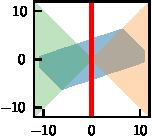
\includegraphics[scale = 0.8,page=1]{images/UVfield.pdf}} \\
\bottomrule
    \end{tabular}
    }
    \caption{Tree-level matching of single-field UV completions \cite{deBlas:2017xtg}
    onto $[O_{\ell q}^{(1)}]_{3333}$ and $[O_{\ell q}^{(3)}]_{3333}$. The penultimate
    column reports the associated perturbative unitarity bound, obtained as the most
    stringent of the constraints for $[C_{\ell q}^{(1)}]_{3333}$ and $[C_{\ell q}^{(3)}]_{3333}$ evaluated on the
    matched Wilson coefficients. The last column contains the plots in the plane $(s[C_{\ell q}^{(1)}]_{3333}/\Lambda^2, s[C_{\ell q}^{(3)}]_{3333}/\Lambda^2)$, where the blue, orange, and green regions correspond to those consistent with unitarity bounds and spin-$0$ and spin-$1$ sum-rule constraints, respectively, while the red lines indicate where each model lies: the scalar and vector leptoquarks are correctly classified by
    their spin, whereas the $t$-channel vectors evade the classification.}
    \label{tab:models}
\end{table}

The two scalar leptoquarks ($\omega_1$, $\zeta$) and the two vector leptoquarks
($\mathcal{U}_2$, $\mathcal{X}$) generate these operators through $s$-channel
exchange in the elastic $\ell q \to \ell q$ amplitude, and therefore enter the
dispersion relation of Eq.~\eqref{eq: sum rules master equation} with their physical
spin. 
Explicitly, the relevant combinations of Table~\ref{tab:sum_rules},
$[C_{\ell q}^{(1)}]_{3333} \pm [C_{\ell q}^{(3)}]_{3333}$, are both non-negative for
$\omega_1$ and $\zeta$, and both non-positive for $\mathcal{U}_2$ and $\mathcal{X}$,
so that the scalar (vector) leptoquarks are correctly placed in the scalar-
(vector-) dominated region of Figure~\ref{fig:3plotsc}.

By contrast, the color-singlet vectors $\mathcal{B} \sim (1,1)_0$ and
$\mathcal{W} \sim (1,3)_0$ couple separately to the lepton and quark currents and are exchanged in the $t$-channel. The boundary terms then no longer vanish, modifying Eq.~\eqref{eq: sum rules master equation}, and the sum-rule
classification fails: $\mathcal{W}$ yields combinations of opposite sign and thus
lies outside both the scalar- and vector-dominated regions, while $\mathcal{B}$ can
fall in the region associated with the opposite (scalar) spin, depending on the sign
of $[g_{\mathcal B}^\ell]_{33}[g_{\mathcal B}^q]_{33}$. These cases provide explicit
examples of the statement made in the main text that vector $t$-channel completions
can violate the spinning sum-rule constraints, whereas all tree-level scalar
completions satisfy them.

\section{Mathematical Tools\label{app:SMEFT_math}}

\subsection{Logical Expression}\label{sec:appendix, logical expression}

In this appendix we prove the statement used in Section~\ref{sec:SMEFT_sumrules}. The function
\begin{equation}
    f(x) = a + bx - \sqrt{c^2 + dx + ex^2}\,,
\end{equation}
assumed real on $[0,1]$ and with $a,b,c,d,e\in\mathbb{R}$, satisfies $f(x) \ge 0$ for every
$x \in [0,1]$ if and only if
\begin{align}
    \Delta(a,b,c,d,e) &= 
    a \ge 0 
    \ \land \
    a+b \ge 0
    \ \land \ 
    a^2 - c^2 \ge 0
    \ \land \ 
    (a+b)^2 - c^2 -d-e \ge 0 \nonumber
    \\& \quad
    \land \
    [e - b^2 \ge 0 \ \lor\  (2ab-d)(2ab-d+2b^2-2e) \ge 0 
    \nonumber \\& \quad
    \lor \ 4(b^2-e)(a^2-c^2)-(2ab-d)^2 \ge 0]
\end{align}
holds, which is the condition quoted in Eq.~\eqref{eq:Delta} of the main text.

Since $g(x)=c^2 + dx + ex^2 \ge 0$ on $[0,1]$ by assumption, $f(x) \ge 0$ on $[0,1]$ is equivalent to $\ell(x) = a + bx \ge 0$ and $h(x) = \ell(x)^2 -g(x) \ge 0$ on $[0,1]$. The latter reads $h(x) = \alpha x^2 + \beta x + \gamma$, with $\alpha = b^2-e$, $\beta = 2ab-d$, and $\gamma=a^2-c^2$.
Thus, it is sufficient to prove that $p(x) = \alpha x^2+\beta x + \gamma \ge 0$ on $[0,1]$ if and only if
    \begin{equation}\label{eq:lemma}
        \gamma\ge0 \ \land \ \alpha+\beta+\gamma\ge0 \ \land \
    [\alpha\le0 \ \lor \ \beta(\beta+2\alpha)\ge0 \ \lor \ 4\alpha\gamma-\beta^2\ge0 ] \,.
    \end{equation}
Indeed, Eq.~\eqref{eq:Delta} is exactly Eq.~\eqref{eq:lemma} applied to $\ell$ and $h$.
The first two conditions in Eq.~\eqref{eq:lemma} are $p(0)\ge 0$ and $p(1)\ge 0$, thus they are necessary; assume them in what follows. If $\alpha \le 0$, then $p$ is concave and has its minimum on $[0,1]$ at an endpoint, so $p\ge 0$; instead, if $\alpha >0$, the vertex is at $x_\ast = -\beta/(2\alpha)$, and
\begin{equation}
    x_\ast\le0 \iff \beta\ge0 \,, \qquad x_\ast\ge1 \iff \beta+2\alpha\le0 \,,
\end{equation}
so $x_\ast \notin (0,1)$ if and only if $\beta(\beta+2\alpha)\ge 0$, in which case the minimum is again at an endpoint and $p\ge 0$. Otherwise, $x_\ast \in (0,1)$ and $\min_{[0,1]} p = p(x_\ast) = (4\alpha\gamma-\beta^2)/(4\alpha)$, which has the same sign as $4\alpha\gamma-\beta^2$. The last condition is then both necessary and sufficient. 

\subsection{Eigenvalues of Jordan--Wielandt Matrices}

Given the Hermitian Jordan--Wielandt matrix
\begin{equation}
    M=\begin{pmatrix}
        \mathbb{O}_{m\times m} & A \\ A^\dagger & \mathbb{O}_{n\times n}
    \end{pmatrix}
\end{equation}
of size $m+n$,
with $A\in \mathbb{C}^{m \times n}$,
we have that its characteristic polynomial --- with the convention $p_X(x) = \det(x\mathbb{1}-X)$ --- is
\begin{equation}
    p_M(x)=x^{n-m}\,p_{AA^\dagger}(x^2) = x^{m-n}\,p_{A^\dagger A}(x^2) \,,
\end{equation}
which means that the eigenvalues of $M$ can be computed as the positive and negative square roots of the eigenvalues of $AA^\dagger$ if $m\le n$ (of $A^\dagger A$ if $m > n$), together with additional $\abs{n-m}$ vanishing eigenvalues. 
%

To prove this, consider a generic block matrix that takes the form
\begin{equation}
    \begin{pmatrix}
        P & Q \\ R & S
    \end{pmatrix}\,.
\end{equation}
If $S$ is invertible, then
\begin{equation}
    \begin{pmatrix}
        P & Q \\ R & S
    \end{pmatrix}
    \begin{pmatrix} \mathbb{1} & \mathbb{O} \\ -S^{-1}R & \mathbb{1} 
    \end{pmatrix}
    =
    \begin{pmatrix} P-QS^{-1}R & Q \\ \mathbb{O} & S 
    \end{pmatrix}\,,
\end{equation}
which implies that 
\begin{equation}
    \det\begin{pmatrix} P & Q \\ R & S \end{pmatrix}=\det(P-QS^{-1}R) \det S \,.
\end{equation}
By applying this to the matrix $x\mathbb{1}_{(m+n)\times(m+n)}-M$, we find the result above.

\section{Complete Results for Flavorful Four-Fermion Operators\label{app:SMEFT_flavorresults}}

In this appendix we collect the marginalized partial-wave unitarity bounds and the corresponding
allowed regions for all the four-fermion operators under the MFV and $U(2)^5$ flavor hypotheses,
obtained with the procedure described in Section~\ref{sec:SMEFT_multiflavor}. For each operator we
report the independent flavor structures and the bound on each independent coefficient.
Table~\ref{tab:summary} serves as an index to the tables and figures that follow. The case of
$O_{\ell q}^{(1,3)}$, used as an illustration in the main text, is reported in
Table~\ref{tab:Olq_UB} and in Figures~\ref{fig:Olq_mfv} and \ref{fig:Olq_u2}.

\begin{table}[tbp]
\renewcommand{\arraystretch}{1.2}
    \centering
    \begin{tabular}{cccc}
    \toprule
    \rowcolor{hdrcolor} \textbf{Operator class}     & \textbf{Operator(s)} & \textbf{Table} & \textbf{Figure(s)}  \\
    \midrule
    \multirow{3}{*}{\boldmath$(\overline LL)(\overline LL)$}     & $O_{\ell \ell}$ &\ref{tab:Oll_UB} & \ref{fig:Oll_mfv} (MFV), \ref{fig:Oll_u2} ($\mathrm{U}(2)^5$)  \\
    & $O_{qq}^{(1,3)}$ &\ref{tab:Oqq_UB}&\ref{fig:Oqq_mfv} (MFV), \ref{fig:Oqq_u2} ($\mathrm{U}(2)^5$) \\
    & $O_{\ell q}^{(1,3)}$ &\ref{tab:Olq_UB}& \ref{fig:Olq_mfv} (MFV), \ref{fig:Olq_u2} ($\mathrm{U}(2)^5$) \\
    \midrule
    \multirow{6}{*}{\boldmath$(\overline RR)(\overline RR)$} & $O_{ee}$ & \ref{tab:Oee_UB} & \ref{fig:Oee_u2} ($\mathrm{U}(2)^5$)  \\
    & $O_{uu}$ &\ref{tab:Ouu_UB}&\ref{fig:Ouu_mfv} (MFV), \ref{fig:Ouu_u2} ($\mathrm{U}(2)^5$) \\
    & $O_{dd}$ &\ref{tab:Odd_UB}& \ref{fig:Odd_mfv} (MFV), \ref{fig:Ouu_u2} ($\mathrm{U}(2)^5$) \\
    & $O_{eu}$ &\ref{tab:Oeu_UB}& \ref{fig:Oeu_mfv} (MFV), \ref{fig:Oeu_u2} ($\mathrm{U}(2)^5$)  \\
    & $O_{ed}$ &\ref{tab:Oed_UB}&  \ref{fig:Oeu_u2} ($\mathrm{U}(2)^5$) \\
    & $O_{ud}^{(1,8)}$ &\ref{tab:Oud_UB}& \ref{fig:Oud_mfv} (MFV), \ref{fig:Oud_u2} ($\mathrm{U}(2)^5$) \\
    \midrule
    \multirow{6}{*}{\boldmath$(\overline LL)(\overline RR)$} & $O_{\ell e}$ &\ref{tab:Ole_UB} &  \ref{fig:Ole_u2} ($\mathrm{U}(2)^5$)  \\
    & $O_{\ell u}$ &\ref{tab:Olu_UB}& \ref{fig:Olu_mfv} (MFV), \ref{fig:Olu_u2} ($\mathrm{U}(2)^5$) \\
    & $O_{\ell d}$ &\ref{tab:Old_UB}&  \ref{fig:Olu_u2} ($\mathrm{U}(2)^5$) \\
    & $O_{qe}$ &\ref{tab:Oqe_UB}& \ref{fig:Oqe_mfv} (MFV), \ref{fig:Oqe_u2} ($\mathrm{U}(2)^5$) \\
    & $O_{qu}^{(1,8)}$ &\ref{tab:Oqu_UB}& \ref{fig:Oqu_mfv} (MFV), \ref{fig:Oqu_u2} ($\mathrm{U}(2)^5$) \\
    & $O_{qd}^{(1,8)}$ &\ref{tab:Oqd_UB}& \ref{fig:Oqd_mfv} (MFV), \ref{fig:Oqu_u2} ($\mathrm{U}(2)^5$) \\
    \bottomrule
    \end{tabular}
    \caption{Hyperlinks to tables of marginalized partial-wave unitarity bounds and figures of the corresponding constraint regions in the MFV and $\mathrm{U}(2)^5$ flavor symmetry scenarios.}
    \label{tab:summary}
\end{table}

\input{tables/tables_flavor_rest}



\begin{figure}[p]
    \centering
    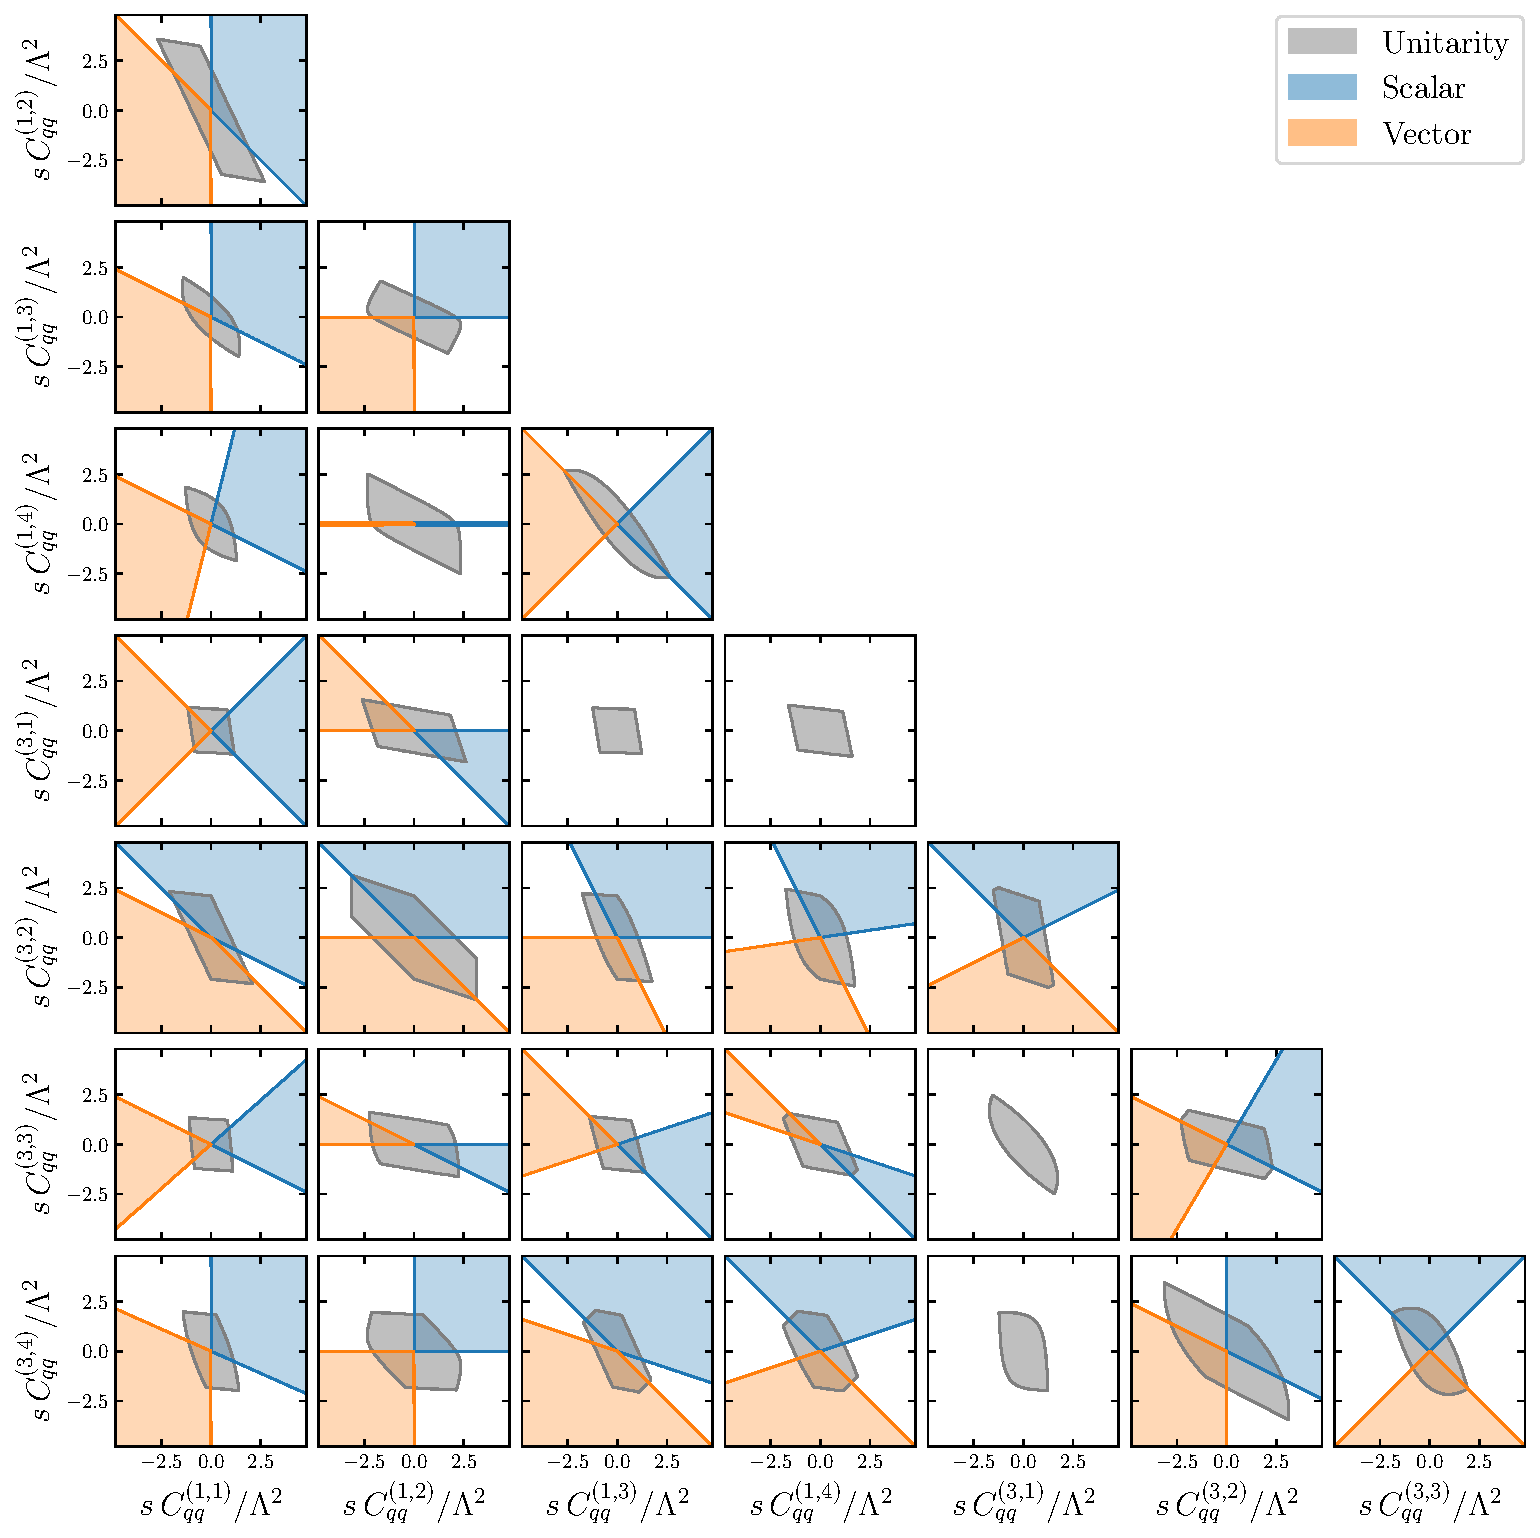
\includegraphics[width=1\linewidth]{images/flavor/Oqq_mfv.pdf}
    \caption{Partial-wave unitarity bounds and sum-rule constraints (under scalar and vector dominance) for the operators $O_{qq}^{(1,3)}$ under MFV, where $[C_{qq}^{(i)}]_{prst} =
            C_{qq}^{(i,1)}\delta_{pr}\delta_{st}
            + C_{qq}^{(i,2)}\delta_{pt}\delta_{sr}
            + C_{qq}^{(i,3)}((Y_u Y_u^\dagger)_{st}\delta_{pr} + (Y_u Y_u^\dagger)_{pr}\delta_{st}) + C_{qq}^{(i,4)}((Y_u Y_u^\dagger)_{sr}\delta_{pt} + (Y_u Y_u^\dagger)_{pt}\delta_{sr})$, $i=1,3$. The regions shown are two-dimensional slices of the full allowed region, obtained by setting to zero all the independent coefficients other than the two displayed.}
    \label{fig:Oqq_mfv}
\end{figure}

\begin{figure}[p]
    \centering
    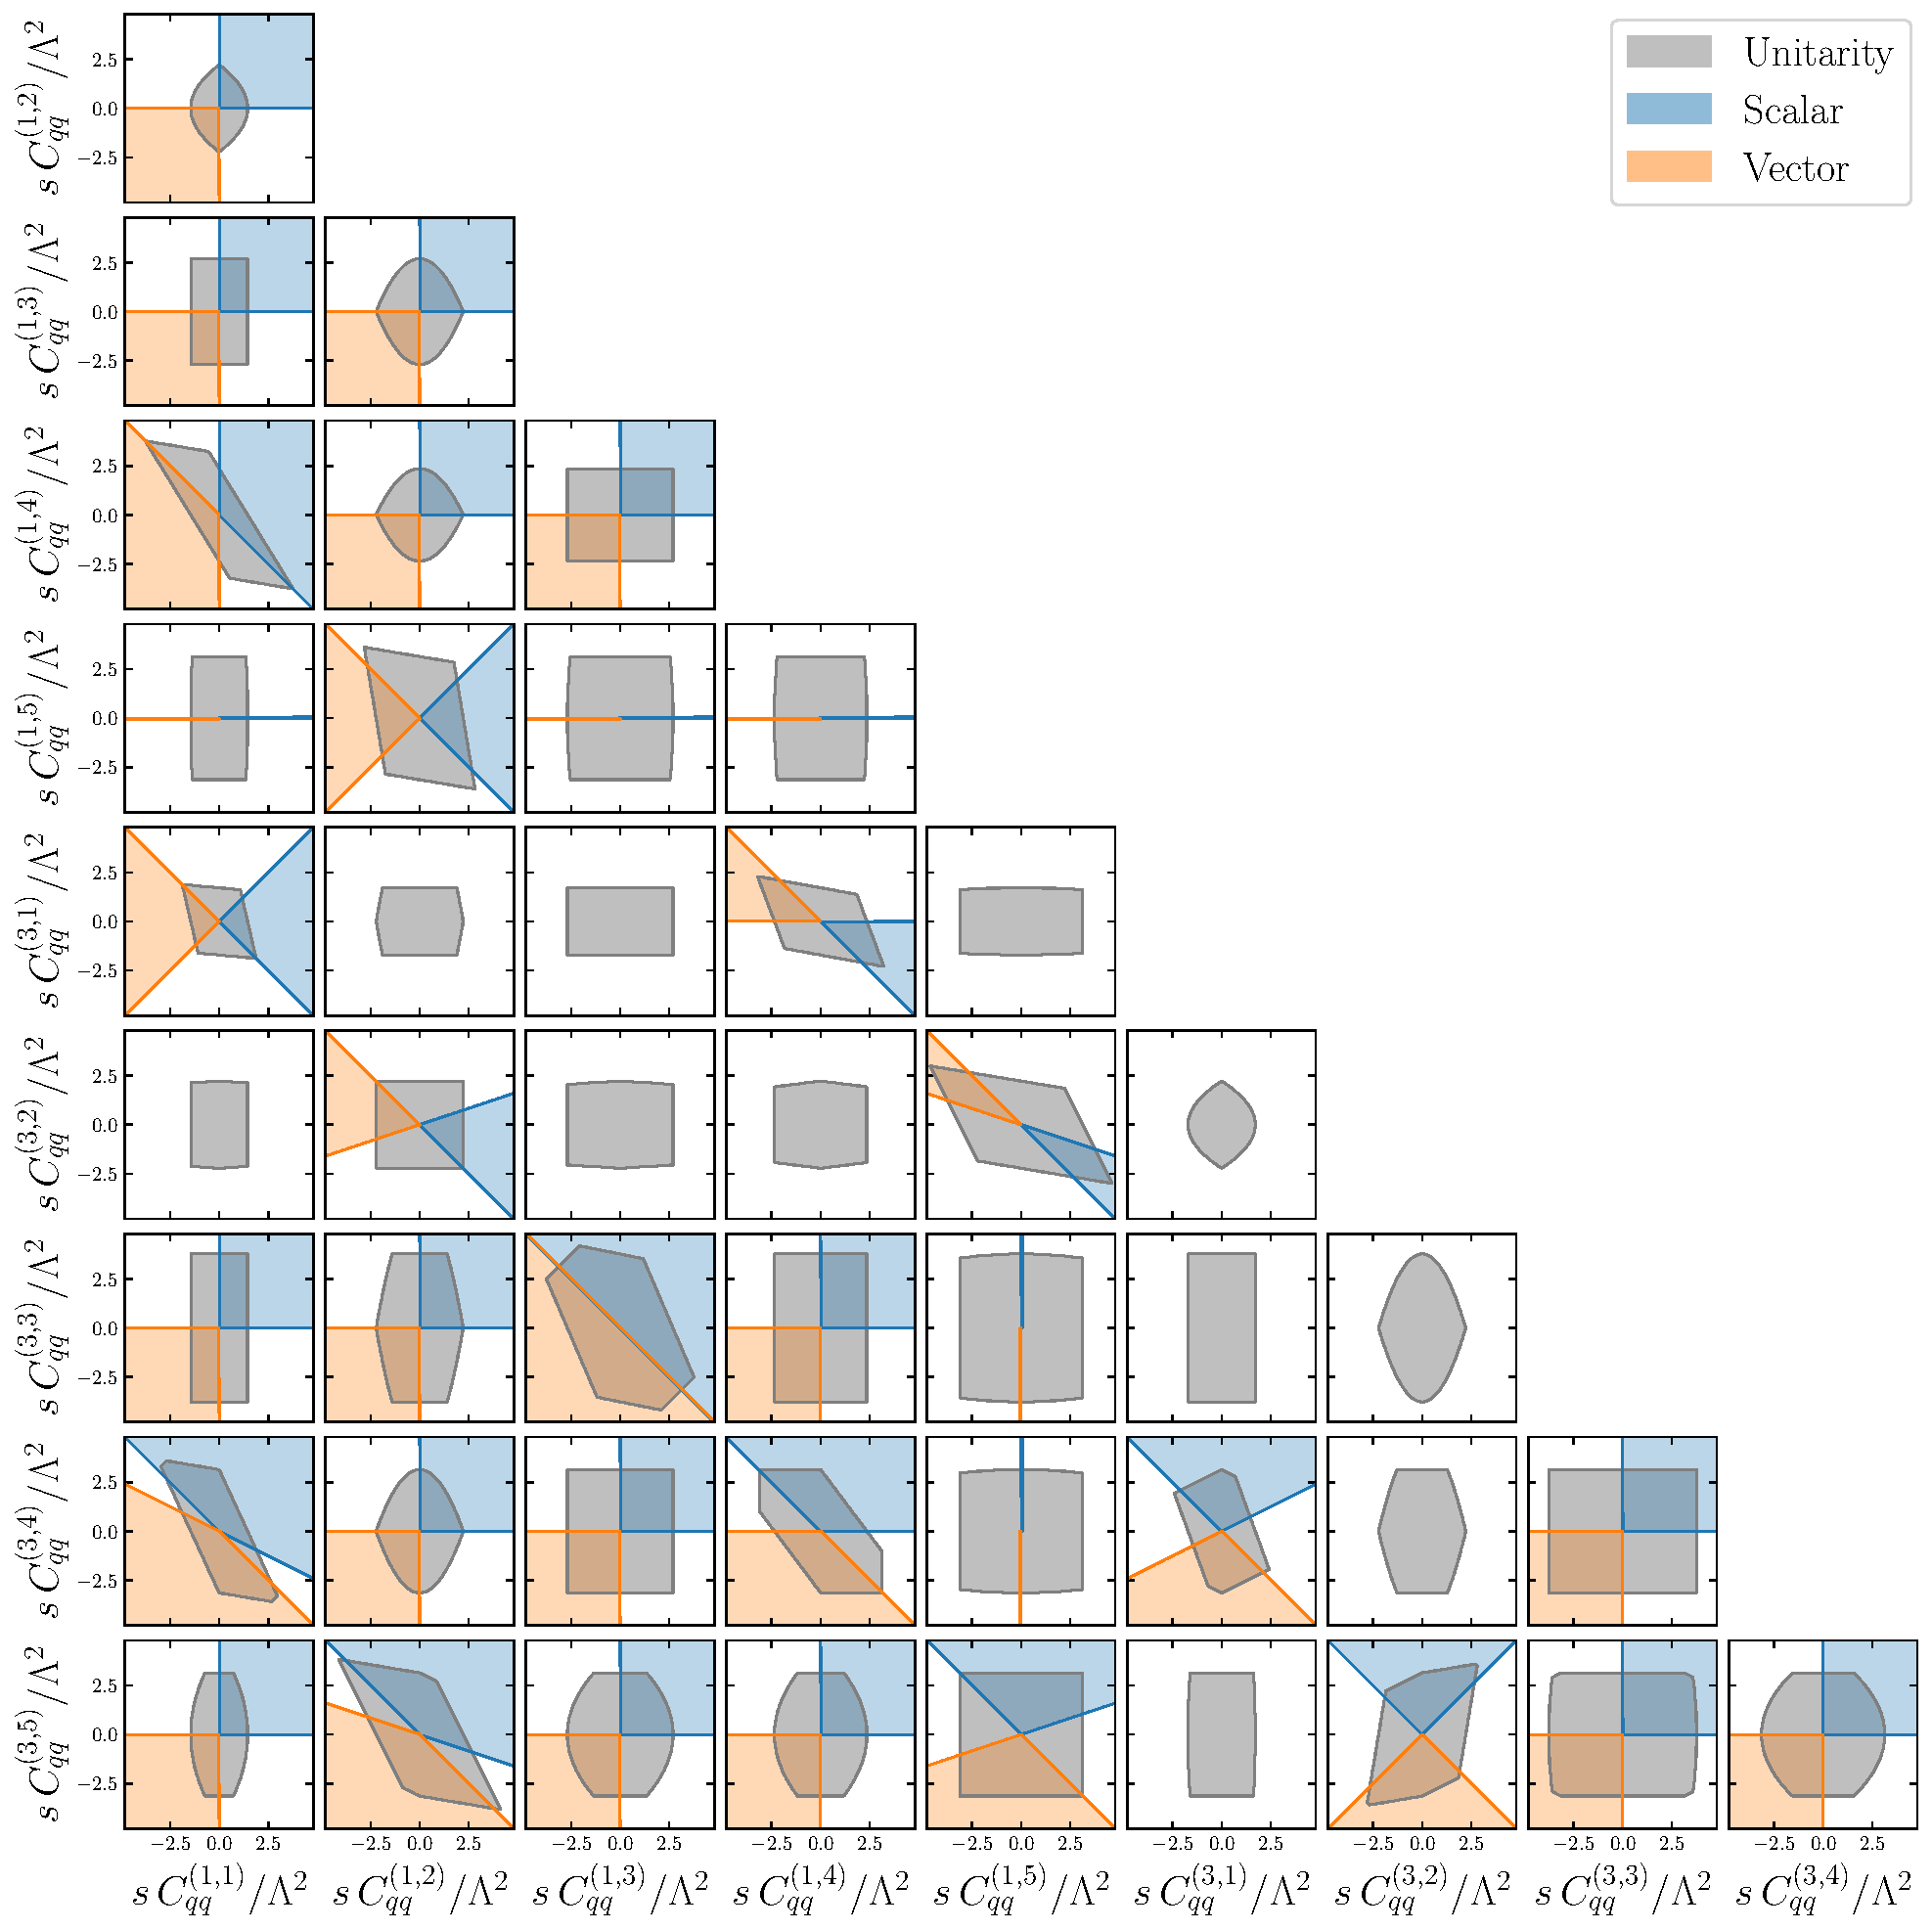
\includegraphics[width=1\linewidth]{images/flavor/Oqq_u2.pdf}
    \caption{Partial-wave unitarity bounds and sum-rule constraints (under scalar and vector dominance) for the operators $O_{qq}^{(i)}$ under $U(2)^5$ flavor symmetry, where $[C_{qq}^{(i)}]_{prst} =
            C_{qq}^{(i,1)}\Pij{p}{r}{a}\Pij{s}{t}{b}
            + C_{qq}^{(i,2)}(\Pij{s}{t}{a}\delta_{p3}\delta_{3r} + \Pij{p}{r}{a}\delta_{s3}\delta_{3t})
            + C_{qq}^{(i,3)}\delta_{p3}\delta_{3r}\delta_{s3}\delta_{3t}
            + C_{qq}^{(i,4)}\Pij{p}{t}{a}\Pij{s}{r}{b}
            + C_{qq}^{(i,5)}(\Pij{s}{r}{a}\delta_{p3}\delta_{3t} + \Pij{p}{t}{a}\delta_{s3}\delta_{3r})$, $i=1,3$. The regions shown are two-dimensional slices of the full allowed region, obtained by setting to zero all the independent coefficients other than the two displayed.}
    \label{fig:Oqq_u2}
\end{figure}

\begin{figure}[p]
    \centering
    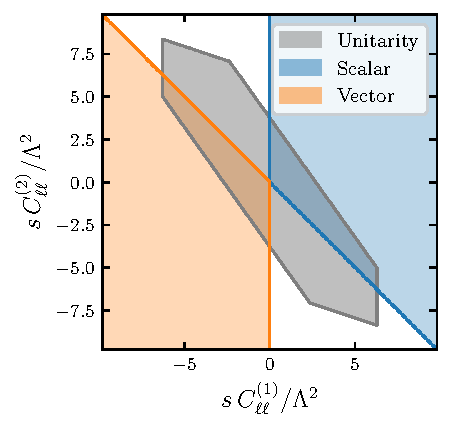
\includegraphics[scale = 0.75]{images/flavor/Oll_mfv.pdf}
    \caption{Partial-wave unitarity bounds and sum-rule constraints (under scalar and vector dominance) for the operator $O_{\ell\ell}$ under MFV, where $[C_{\ell\ell}]_{prst} = C_{\ell\ell}^{(1)}\delta_{pr}\delta_{st} + C_{\ell\ell}^{(2)}\delta_{pt}\delta_{rs}$.}
    \label{fig:Oll_mfv}
\end{figure}

\begin{figure}[p]
    \centering
    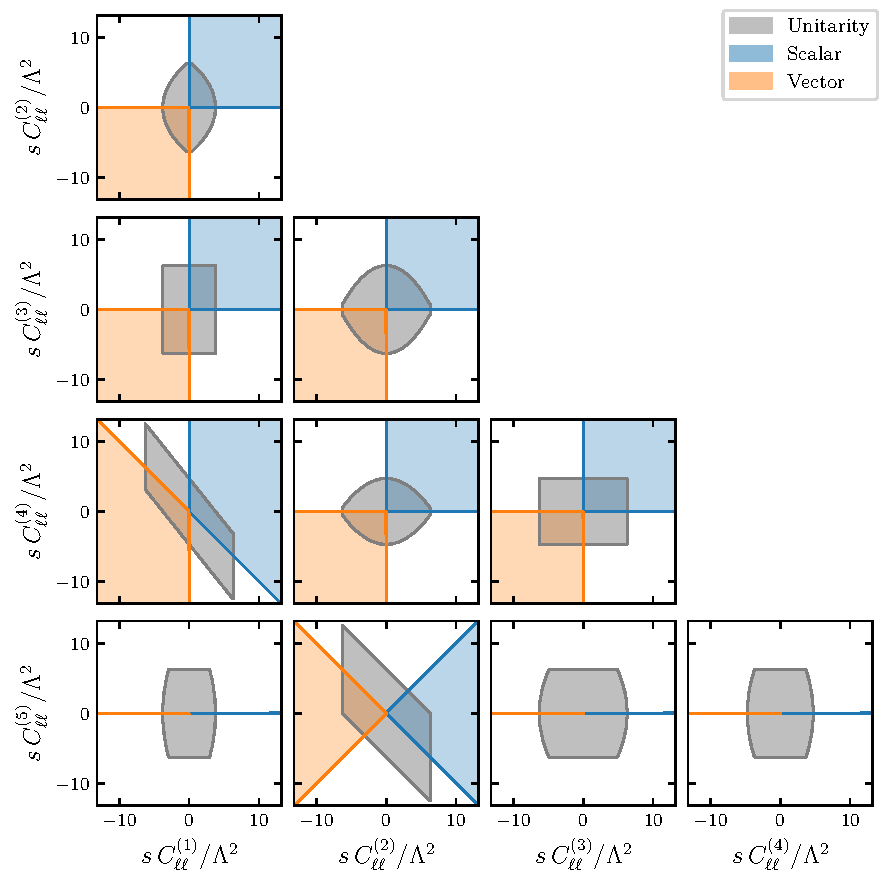
\includegraphics[scale = 0.75]{images/flavor/Oll_u2.pdf}
    \caption{Partial-wave unitarity bounds and sum-rule constraints (under scalar and vector dominance) for the operator $O_{\ell\ell}$ under $U(2)^5$ flavor symmetry, where $[C_{\ell\ell}]_{prst} =
            C_{\ell\ell}^{(1)}\Pij{p}{r}{a}\Pij{s}{t}{b}
            + C_{\ell\ell}^{(2)}(\Pij{s}{t}{a}\delta_{p3}\delta_{3r} + \Pij{p}{r}{a}\delta_{s3}\delta_{3t})
            + C_{\ell\ell}^{(3)}\delta_{p3}\delta_{3r}\delta_{s3}\delta_{3t}
            + C_{\ell\ell}^{(4)}\Pij{s}{r}{a}\Pij{p}{t}{b}
            + C_{\ell\ell}^{(5)}(\Pij{p}{t}{a}\delta_{s3}\delta_{3r} + \Pij{s}{r}{a}\delta_{p3}\delta_{3t})$. The regions shown are two-dimensional slices of the full allowed region, obtained by setting to zero all the independent coefficients other than the two displayed.}
    \label{fig:Oll_u2}
\end{figure}

\begin{figure}[p]
    \centering
    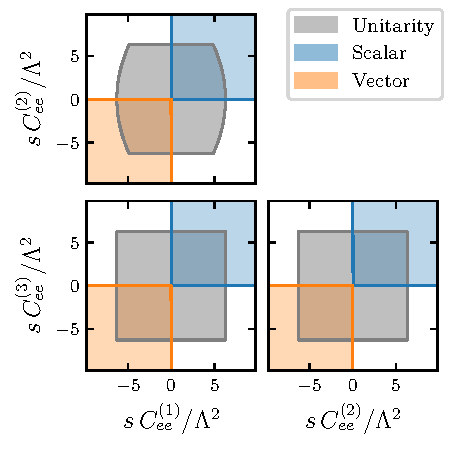
\includegraphics[scale = 0.75]{images/flavor/Oee_u2.pdf}
    \caption{Partial-wave unitarity bounds and sum-rule constraints (under scalar and vector dominance) for the operator $O_{ee}$ under $U(2)^5$ flavor symmetry, where $[C_{ee}]_{prst} =
            C_{ee}^{(1)}\Pij{p}{r}{a}\Pij{s}{t}{b}
            + C_{ee}^{(2)}(\Pij{s}{t}{a}\delta_{p3}\delta_{3r} + \Pij{p}{r}{a}\delta_{s3}\delta_{3t}) + C_{ee}^{(3)}\delta_{p3}\delta_{3r}\delta_{s3}\delta_{3t}$. The regions shown are two-dimensional slices of the full allowed region, obtained by setting to zero all the independent coefficients other than the two displayed.}
    \label{fig:Oee_u2}
\end{figure}

\begin{figure}[p]
    \centering
    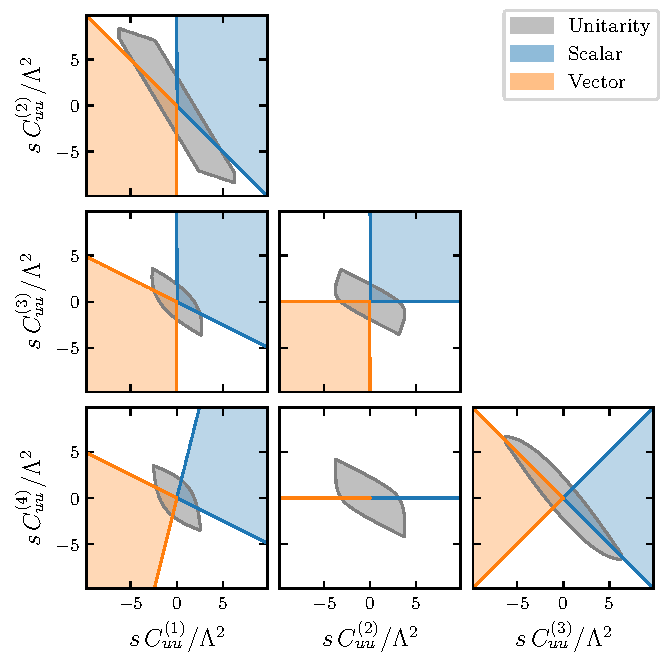
\includegraphics[scale = 0.75]{images/flavor/Ouu_mfv.pdf}
    \caption{Partial-wave unitarity bounds and sum-rule constraints (under scalar and vector dominance) for the operators $O_{uu}$ under MFV, where $[C_{uu}]_{prst} =
            C_{uu}^{(1)}\delta_{pr}\delta_{st}
            + C_{uu}^{(2)}\delta_{pt}\delta_{sr}
            + C_{uu}^{(3)}((Y_u^\dagger Y_u)_{st}\delta_{pr} + (Y_u^\dagger Y_u)_{pr}\delta_{st})+ C_{uu}^{(4)}((Y_u^\dagger Y_u)_{sr}\delta_{pt} + (Y_u^\dagger Y_u)_{pt}\delta_{sr})$. The regions shown are two-dimensional slices of the full allowed region, obtained by setting to zero all the independent coefficients other than the two displayed.}
    \label{fig:Ouu_mfv}
\end{figure}

\begin{figure}[p]
    \centering
    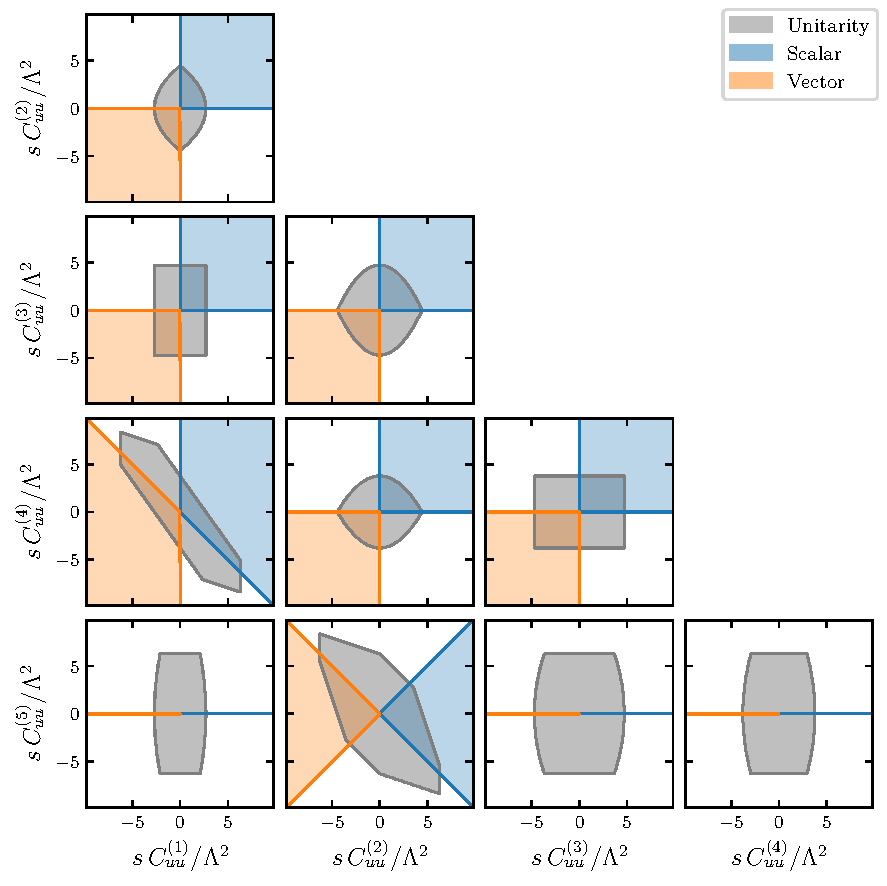
\includegraphics[scale = 0.75]{images/flavor/Ouu_u2.pdf}
    \caption{Partial-wave unitarity bounds and sum-rule constraints (under scalar and vector dominance) for the operators $O_{uu}$ under $U(2)^5$ flavor symmetry, where $[C_{uu}]_{prst} =
            C_{uu}^{(1)}\Pij{p}{r}{a}\Pij{s}{t}{b}
            + C_{uu}^{(2)}(\Pij{s}{t}{a}\delta_{p3}\delta_{3r} + \Pij{p}{r}{a}\delta_{s3}\delta_{3t})
            + C_{uu}^{(3)}\delta_{p3}\delta_{3r}\delta_{s3}\delta_{3t}
            + C_{uu}^{(4)}\Pij{p}{t}{a}\Pij{s}{r}{b}
            + C_{uu}^{(5)}(\Pij{s}{r}{a}\delta_{p3}\delta_{3t} + \Pij{p}{t}{a}\delta_{s3}\delta_{3r})$. Same decomposition and plots are valid also for $O_{dd}$. The regions shown are two-dimensional slices of the full allowed region, obtained by setting to zero all the independent coefficients other than the two displayed.}
    \label{fig:Ouu_u2}
\end{figure}

\begin{figure}[p]
    \centering
    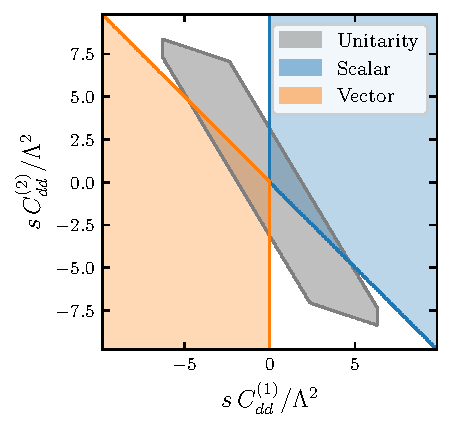
\includegraphics[scale = 0.75]{images/flavor/Odd_mfv.pdf}
    \caption{Partial-wave unitarity bounds and sum-rule constraints (under scalar and vector dominance) for the operators $O_{dd}$ under MFV, where $[C_{dd}]_{prst} =
            C_{dd}^{(1)}\delta_{pr}\delta_{st}
            + C_{dd}^{(2)}\delta_{pt}\delta_{sr}
            $.}
    \label{fig:Odd_mfv}
\end{figure}

\begin{figure}[p]
    \centering
    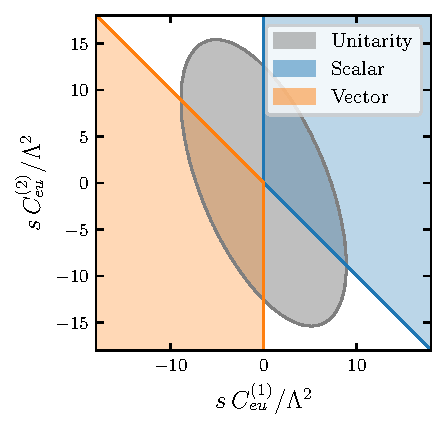
\includegraphics[scale = 0.75]{images/flavor/Oeu_mfv.pdf}
    \caption{Partial-wave unitarity bounds and sum-rule constraints (under scalar and vector dominance) for the operators $O_{eu}$ under MFV, where $[C_{eu}]_{prst} =
            C_{eu}^{(1)}\delta_{pr}\delta_{st}
            + C_{eu}^{(2)}\delta_{pr}(Y_u^\dagger Y_u)_{st}
            $.}
    \label{fig:Oeu_mfv}
\end{figure}

\begin{figure}[p]
    \centering
    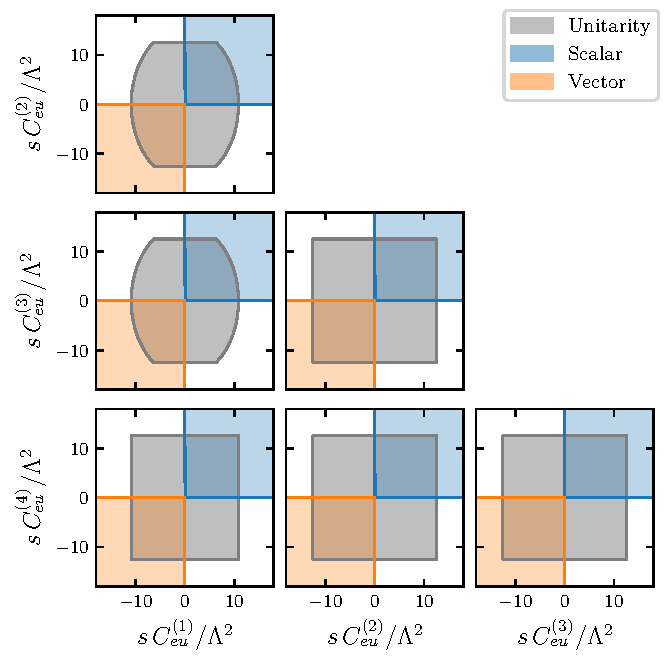
\includegraphics[scale = 0.75]{images/flavor/Oeu_u2.pdf}
    \caption{Partial-wave unitarity bounds and sum-rule constraints (under scalar and vector dominance) for the operators $O_{eu}$ under $U(2)^5$ flavor symmetry, where $[C_{eu}]_{prst} =
            C_{eu}^{(1)}\Pij{p}{r}{a}\Pij{s}{t}{b}
            + C_{eu}^{(2)}\delta_{p3}\delta_{3r}\Pij{s}{t}{a} + C_{eu}^{(3)}\delta_{s3}\delta_{3t}\Pij{p}{r}{a}
            + C_{eu}^{(4)}\delta_{p3}\delta_{3r}\delta_{s3}\delta_{3t}$. Same decomposition and plots are valid also for $O_{ed}$. The regions shown are two-dimensional slices of the full allowed region, obtained by setting to zero all the independent coefficients other than the two displayed.}
    \label{fig:Oeu_u2}
\end{figure}

\begin{figure}[p]
    \centering
    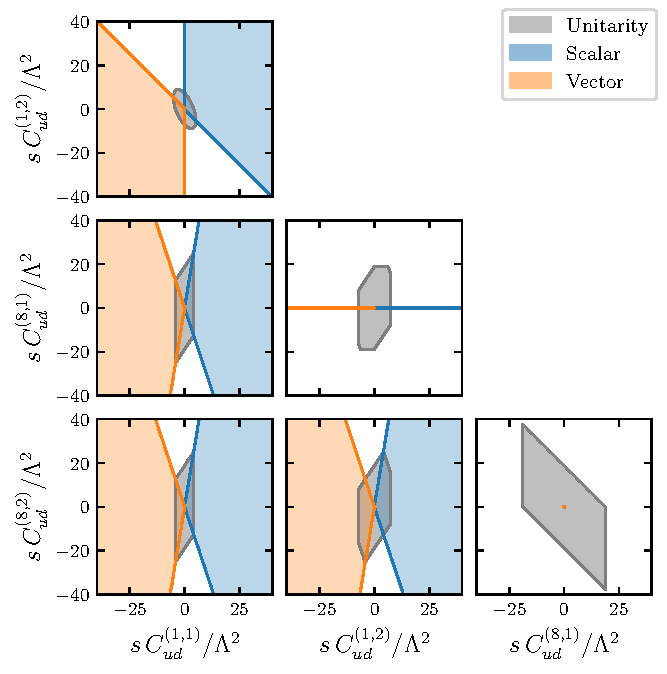
\includegraphics[scale = 0.75]{images/flavor/Oud_mfv.pdf}
    \caption{Partial-wave unitarity bounds and sum-rule constraints (under scalar and vector dominance) for the operators $O_{ud}^{(1,8)}$ under MFV, where $[C_{ud}^{(i)}]_{prst} =
            C_{ud}^{(i,1)}\delta_{pr}\delta_{st}
            + C_{ud}^{(i,2)}(Y_u^\dagger Y_u)_{pr}\delta_{st}$, $i=1,8$. The regions shown are two-dimensional slices of the full allowed region, obtained by setting to zero all the independent coefficients other than the two displayed.}
    \label{fig:Oud_mfv}
\end{figure}

\begin{figure}[p]
    \centering
    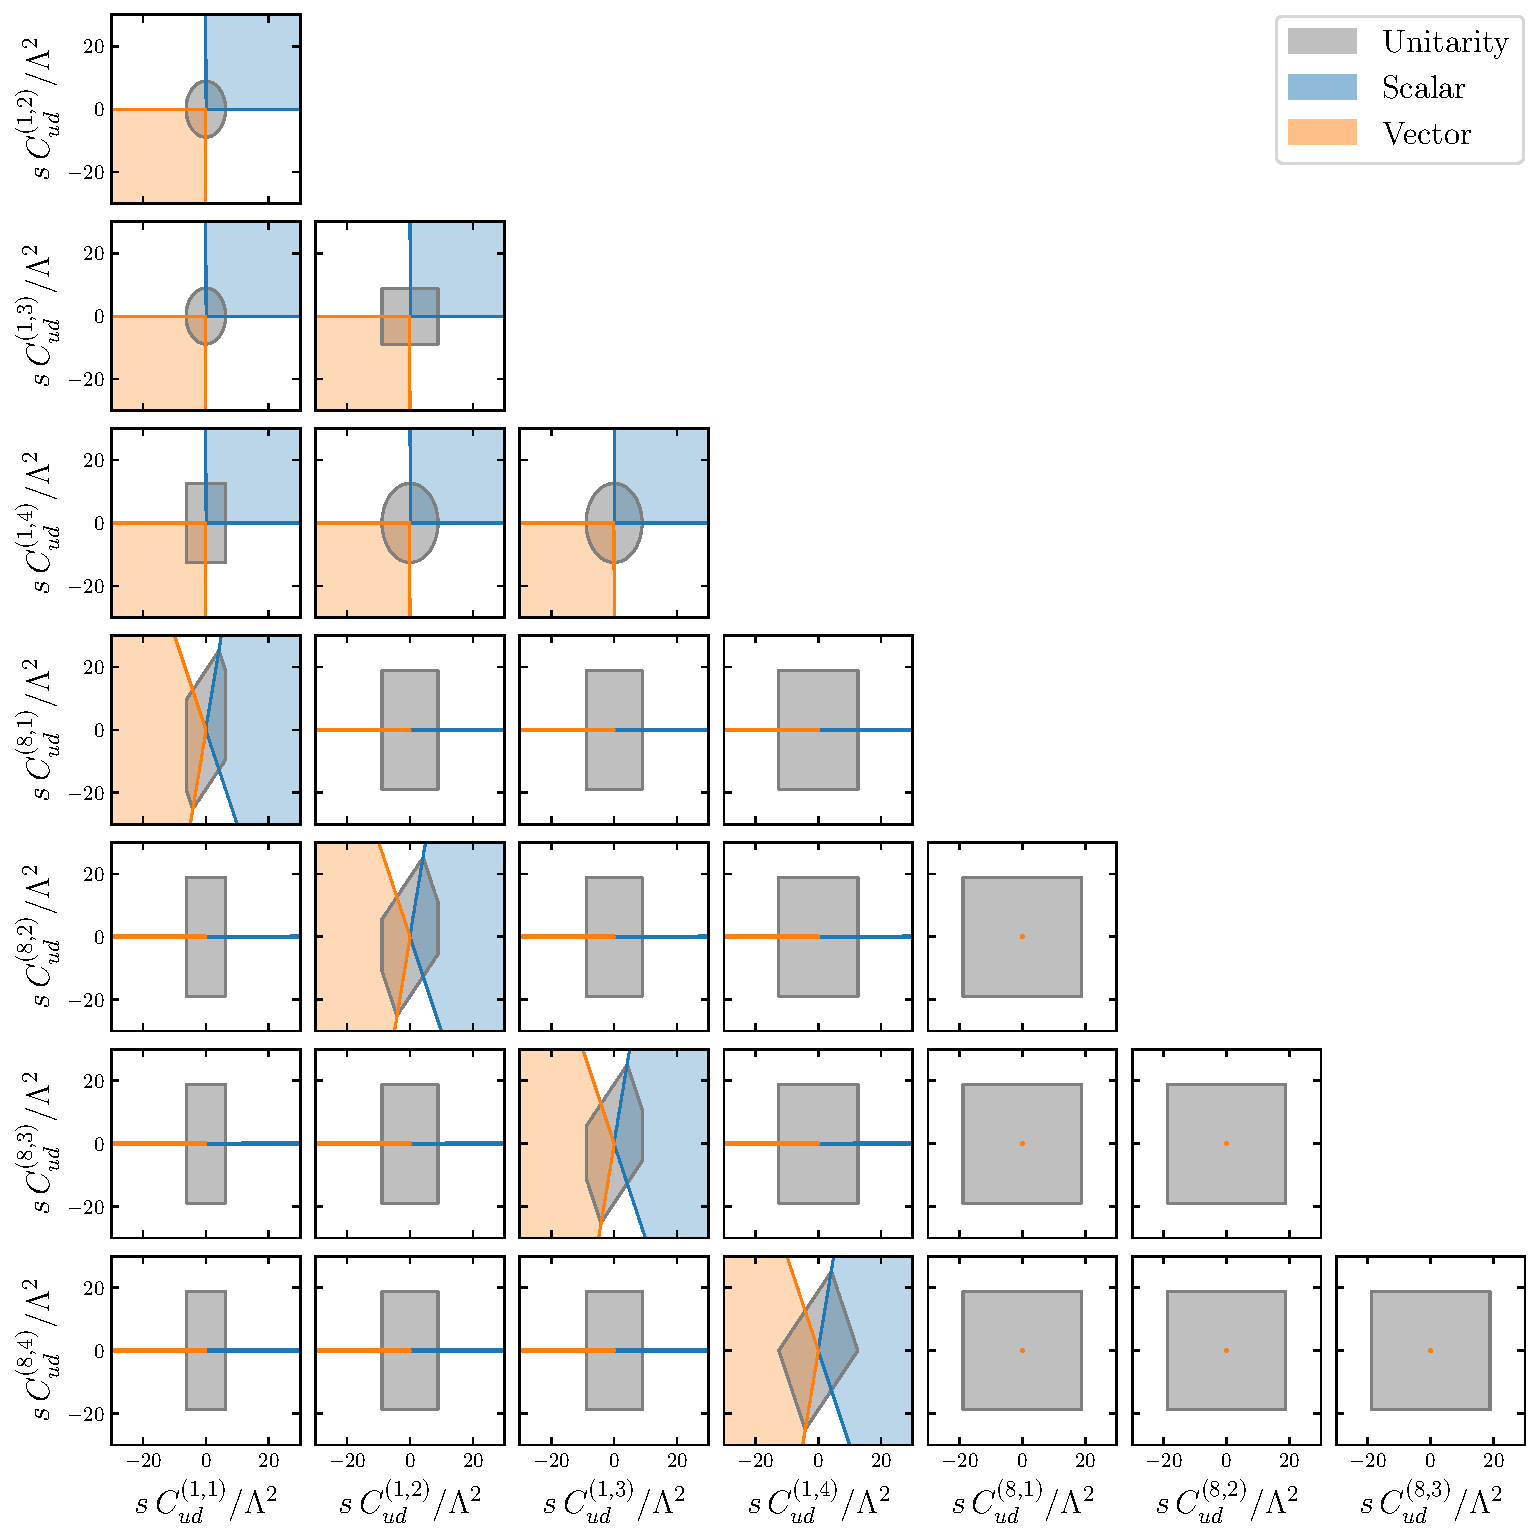
\includegraphics[width=\linewidth]{images/flavor/Oud_u2.pdf}
    \caption{Partial-wave unitarity bounds and sum-rule constraints (under scalar and vector dominance) for the operators $O_{ud}^{(1,8)}$ under $U(2)^5$ flavor symmetry, where $[C_{ud}^{(i)}]_{prst} =
            C_{ud}^{(i,1)}\Pij{p}{r}{a}\Pij{s}{t}{b}
            + C_{ud}^{(i,2)}\Pij{s}{t}{a}\delta_{p3}\delta_{3r}+ C_{ud}^{(i,3)}\Pij{p}{r}{a}\delta_{s3}\delta_{3t}
            + C_{ud}^{(i,4)}\delta_{p3}\delta_{3r}\delta_{s3}\delta_{3t}$, $i=1,8$. The regions shown are two-dimensional slices of the full allowed region, obtained by setting to zero all the independent coefficients other than the two displayed.}
    \label{fig:Oud_u2}
\end{figure}

\begin{figure}[p]
    \centering
    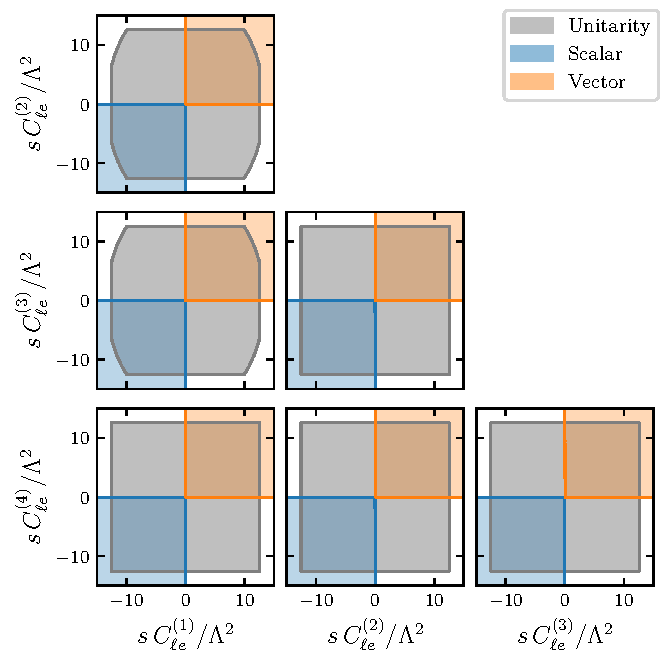
\includegraphics[scale = 0.75]{images/flavor/Ole_u2.pdf}
    \caption{Partial-wave unitarity bounds and sum-rule constraints (under scalar and vector dominance) for the operators $O_{\ell e}$ under $U(2)^5$ flavor symmetry, where $[C_{\ell e}]_{prst} =
            C_{\ell e}^{(1)}\Pij{p}{r}{a}\Pij{s}{t}{a}
            + C_{\ell e}^{(2)}\Pij{s}{t}{a}\delta_{p3}\delta_{3r}+ C_{\ell e}^{(3)}\Pij{p}{r}{a}\delta_{s3}\delta_{3t}
            + C_{\ell e}^{(4)}\delta_{p3}\delta_{3r}\delta_{s3}\delta_{3t}$. The regions shown are two-dimensional slices of the full allowed region, obtained by setting to zero all the independent coefficients other than the two displayed.}
    \label{fig:Ole_u2}
\end{figure}

\begin{figure}[p]
    \centering
    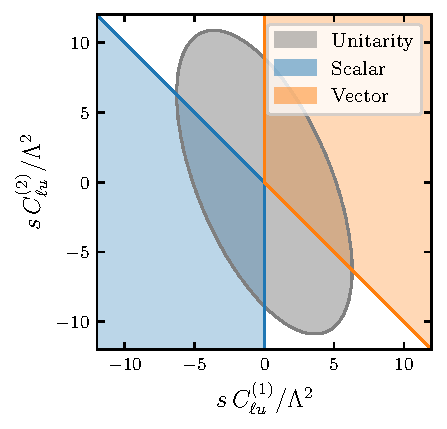
\includegraphics[scale = 0.75]{images/flavor/Olu_mfv.pdf}
    \caption{Partial-wave unitarity bounds and sum-rule constraints (under scalar and vector dominance) for the operators $O_{\ell u}$ under MFV, where $[C_{\ell u}]_{prst} = C_{\ell u}^{(1)}\delta_{pr}\delta_{st} + C_{\ell u}^{(2)}\delta_{pr}(Y_u^\dagger Y_u)_{st}$.}
    \label{fig:Olu_mfv}
\end{figure}

\begin{figure}[p]
    \centering
    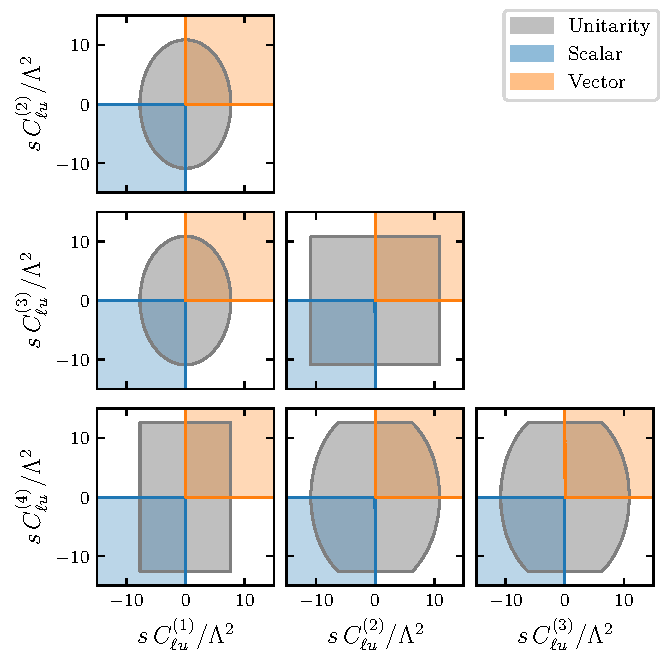
\includegraphics[scale = 0.75]{images/flavor/Olu_u2.pdf}
    \caption{Partial-wave unitarity bounds and sum-rule constraints (under scalar and vector dominance) for the operators $O_{\ell u}$ under $U(2)^5$ flavor symmetry, where $[C_{\ell u}]_{prst} =
            C_{\ell u}^{(1)}\Pij{p}{r}{a}\Pij{s}{t}{a}
            + C_{\ell u}^{(2)}\Pij{s}{t}{a}\delta_{p3}\delta_{3r}+ C_{\ell u}^{(3)}\Pij{p}{r}{a}\delta_{s3}\delta_{3t}
            + C_{\ell u}^{(4)}\delta_{p3}\delta_{3r}\delta_{s3}\delta_{3t}$. Same decomposition and plots are valid also for $O_{\ell d}$. The regions shown are two-dimensional slices of the full allowed region, obtained by setting to zero all the independent coefficients other than the two displayed.}
    \label{fig:Olu_u2}
\end{figure}

\begin{figure}[p]
    \centering
    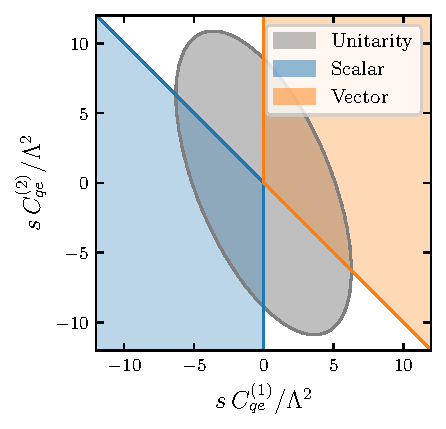
\includegraphics[scale = 0.75]{images/flavor/Oqe_mfv.pdf}
    \caption{Partial-wave unitarity bounds and sum-rule constraints (under scalar and vector dominance) for the operators $O_{qe}$ under MFV, where $[C_{qe}]_{prst} = C_{qe}^{(1)}\delta_{pr}\delta_{st} + C_{qe}^{(2)}(Y_u Y_u^\dagger)_{pr}\delta_{st}$.}
    \label{fig:Oqe_mfv}
\end{figure}

\begin{figure}[p]
    \centering
    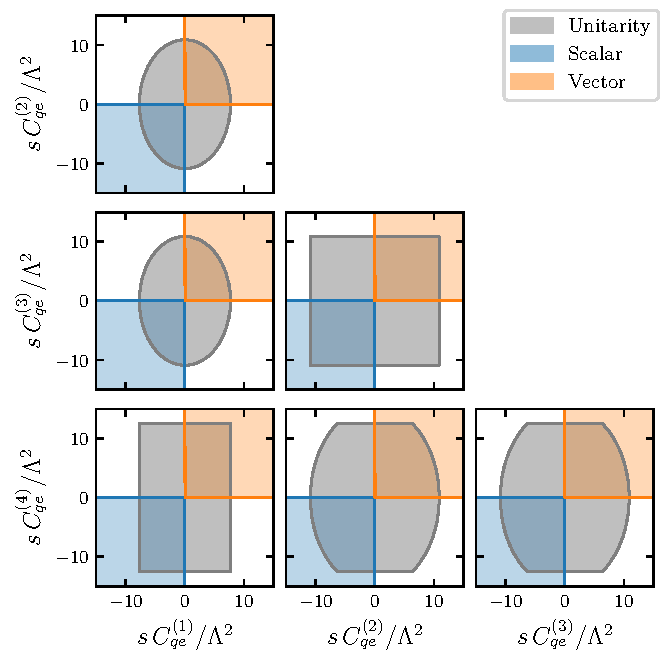
\includegraphics[scale = 0.75]{images/flavor/Oqe_u2.pdf}
    \caption{Partial-wave unitarity bounds and sum-rule constraints (under scalar and vector dominance) for the operators $O_{qe}$ under $U(2)^5$ flavor symmetry, where $[C_{qe}]_{prst} =
            C_{qe}^{(1)}\Pij{p}{r}{a}\Pij{s}{t}{a}
            + C_{qe}^{(2)}\Pij{s}{t}{a}\delta_{p3}\delta_{3r}+ C_{qe}^{(3)}\Pij{p}{r}{a}\delta_{s3}\delta_{3t}
            + C_{qe}^{(4)}\delta_{p3}\delta_{3r}\delta_{s3}\delta_{3t}$. The regions shown are two-dimensional slices of the full allowed region, obtained by setting to zero all the independent coefficients other than the two displayed.}
    \label{fig:Oqe_u2}
\end{figure}

\begin{figure}[p]
    \centering
    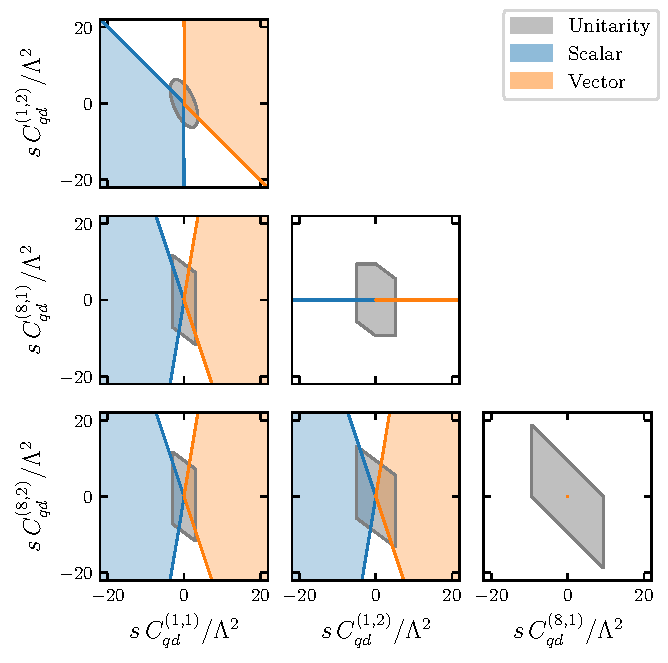
\includegraphics[scale = 0.75]{images/flavor/Oqd_mfv.pdf}
    \caption{Partial-wave unitarity bounds and sum-rule constraints (under scalar and vector dominance) for the operators $O_{qd}^{(1,8)}$ under MFV, where $[C_{qd}^{(i)}]_{prst} =
            C_{qd}^{(i,1)}\delta_{pr}\delta_{st}
            + C_{qd}^{(i,2)}(Y_u Y_u^\dagger)_{pr}\delta_{st}$, $i=1,8$. The regions shown are two-dimensional slices of the full allowed region, obtained by setting to zero all the independent coefficients other than the two displayed.}
    \label{fig:Oqd_mfv}
\end{figure}

\begin{figure}[p]
    \centering
    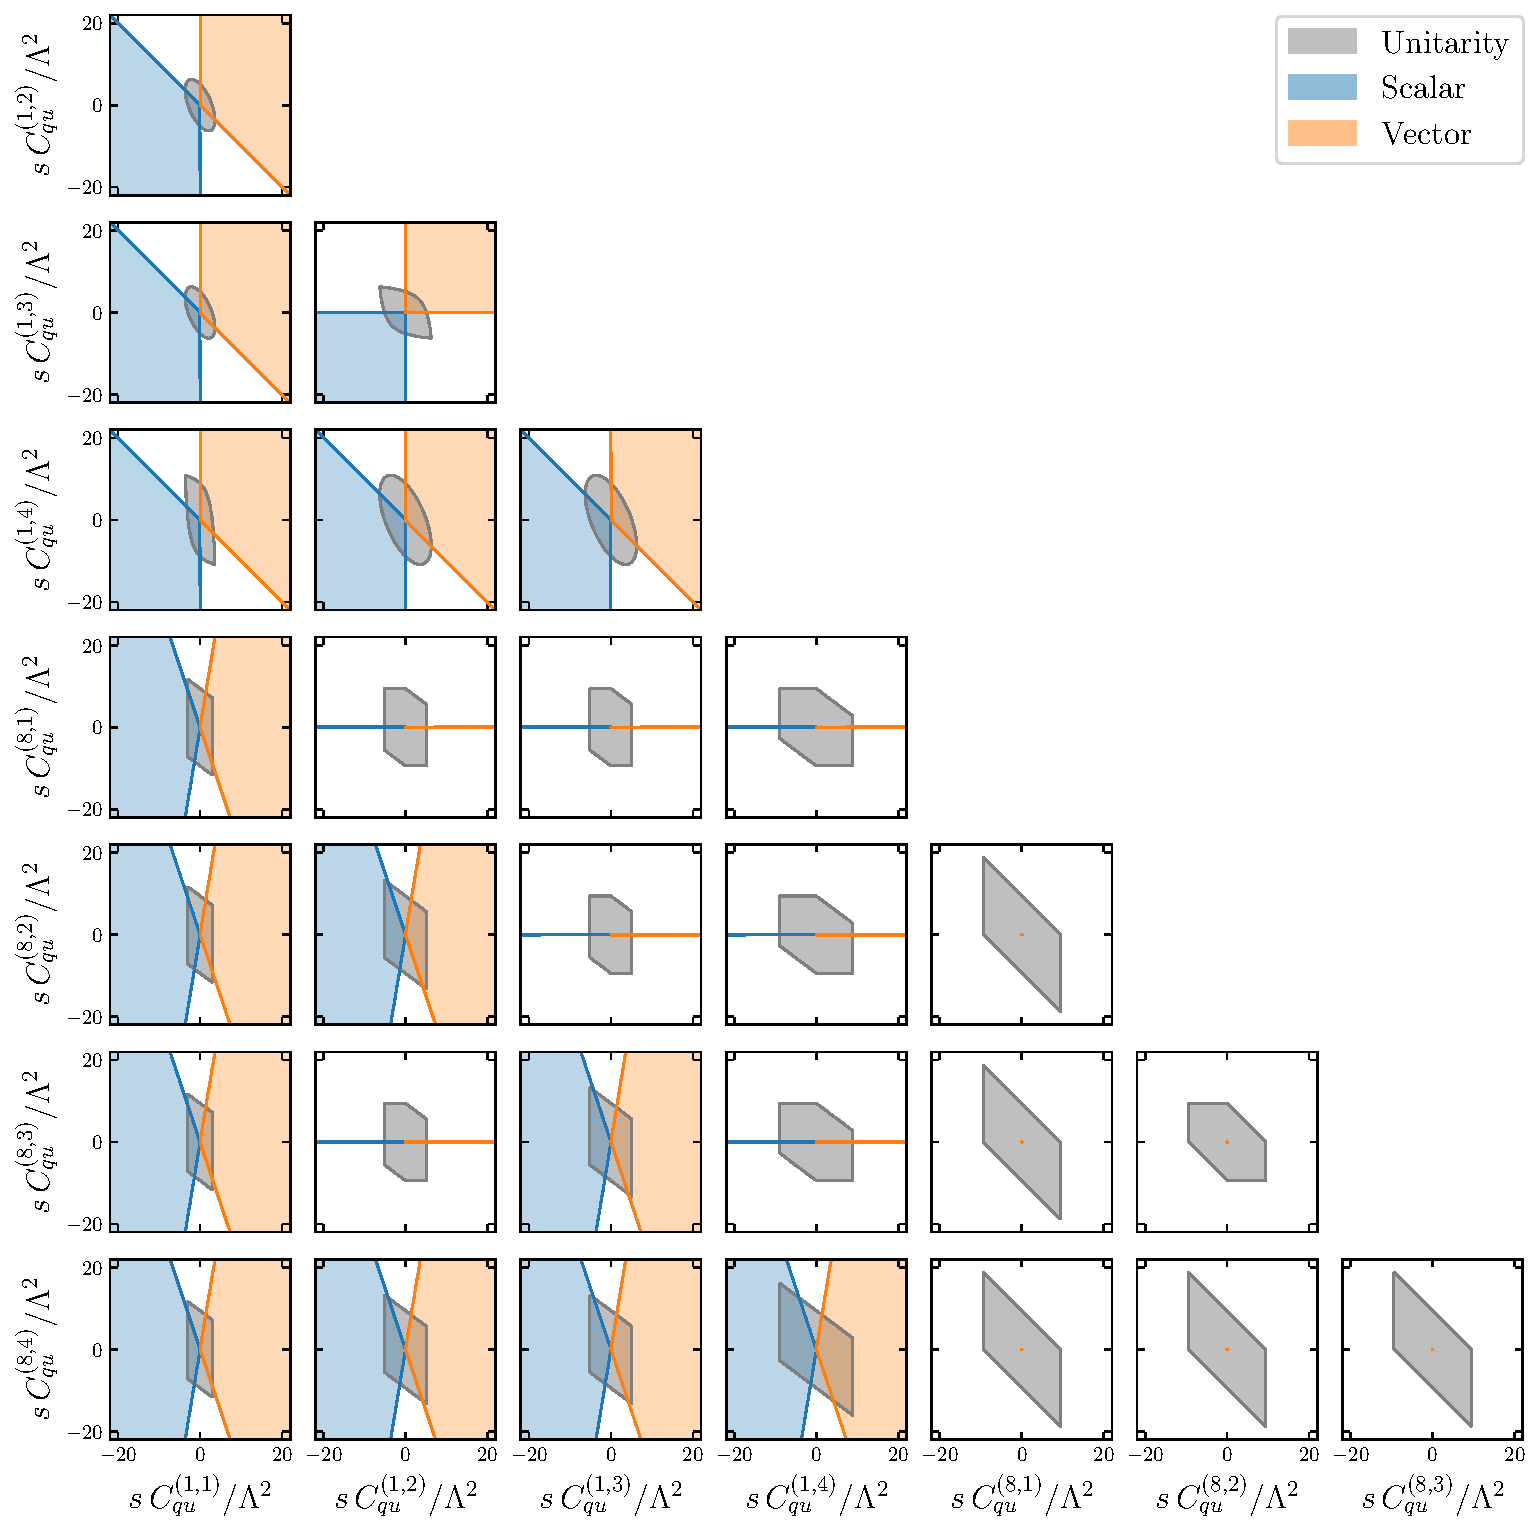
\includegraphics[width=\linewidth]{images/flavor/Oqu_mfv.pdf}
    \caption{Partial-wave unitarity bounds and sum-rule constraints (under scalar and vector dominance) for the operators $O_{qu}^{(1,8)}$ under MFV, where $[C_{qu}^{(i)}]_{prst} =
            C_{qu}^{(i,1)}\delta_{pr}\delta_{st}
            + C_{qu}^{(i,2)}(Y_u Y_u^\dagger)_{pr}\delta_{st}+ C_{qu}^{(i,3)}\delta_{pr}(Y_u^\dagger Y_u)_{st}
            + C_{qu}^{(i,4)}(Y_u)_{pt}(Y_u^\dagger)_{sr}$, $i=1,8$. The regions shown are two-dimensional slices of the full allowed region, obtained by setting to zero all the independent coefficients other than the two displayed.}
    \label{fig:Oqu_mfv}
\end{figure}

\begin{figure}[p]
    \centering
    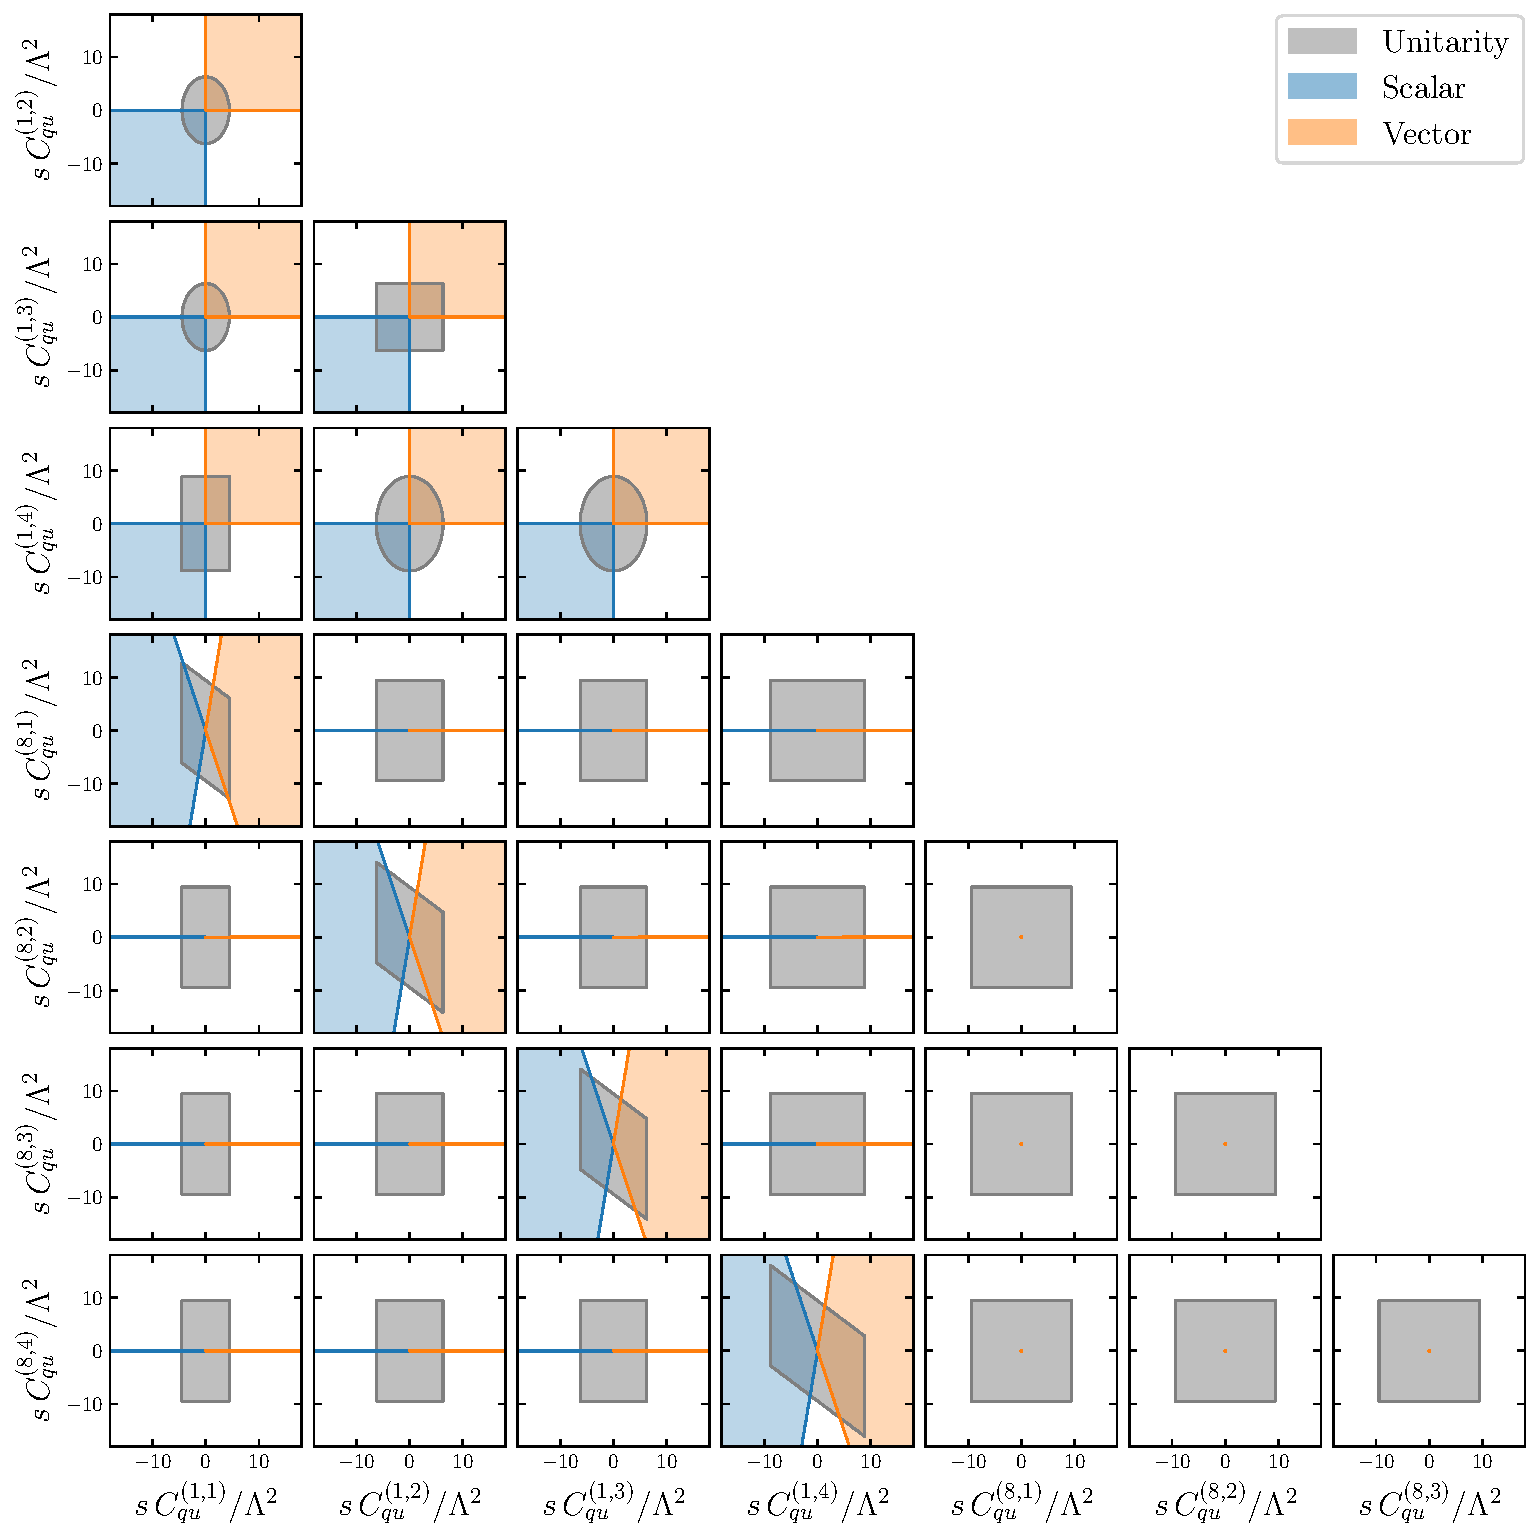
\includegraphics[width=\linewidth]{images/flavor/Oqu_u2.pdf}
    \caption{Partial-wave unitarity bounds and sum-rule constraints (under scalar and vector dominance) for the operators $O_{qu}^{(1,8)}$ under $U(2)^5$ flavor symmetry, where $[C_{qu}^{(i)}]_{prst} =
            C_{qu}^{(i,1)}\Pij{p}{r}{a}\Pij{s}{t}{a}
            + C_{qu}^{(i,2)}\Pij{s}{t}{a}\delta_{p3}\delta_{3r}+ C_{qu}^{(i,3)}\Pij{p}{r}{a}\delta_{s3}\delta_{3t}
            + C_{qu}^{(i,4)}\delta_{p3}\delta_{3r}\delta_{s3}\delta_{3t}$, $i=1,8$. Same decomposition and plots are valid also for $O_{qd}^{(1,8)}$. The regions shown are two-dimensional slices of the full allowed region, obtained by setting to zero all the independent coefficients other than the two displayed.}
    \label{fig:Oqu_u2}
\end{figure}


\end{subappendices}



%\part*{Back Matter\phantomsection\addcontentsline{toc}{part}{Back Matter}}

\part{Final Remarks}

\chapter{Conclusions}

Effective Field Theories (EFTs) provide the most general and systematic way to describe a physical
system at energies below the characteristic scale of a more fundamental theory, encoding the
indirect effects of the heavy degrees of freedom in the coefficients of higher-dimensional
operators. Among the many EFTs developed in particle physics, those describing
beyond-the-Standard-Model effects are of particular interest. The Standard Model Effective Field
Theory (SMEFT) plays a key role, being the most general local, Lorentz-invariant effective theory
built from the Standard Model field content and invariant under its gauge group, with the Higgs in a
linearly realized $SU(2)_L$ doublet. Another widely studied example is the EFT of axion-like
particles (ALPs), which introduces a light pseudoscalar field whose interactions are suppressed by a
high-energy scale. Such fields naturally arise in theories with spontaneously broken approximate
global symmetries, where the ALP plays the role of a pseudo-Nambu--Goldstone boson, and they provide
a compelling framework to address several open questions in particle physics, such as the strong CP
problem, the flavor puzzle, the nature of dark matter, and the electroweak-scale naturalness
problem.

Within the EFT framework, the Wilson coefficients of higher-dimensional operators are
scale-dependent couplings that encode heavy-physics effects, and fundamental principles impose
non-trivial constraints on their allowed values. Therefore, to connect experimental data with the
underlying high-energy physics, it is essential to determine:
\begin{itemize}
    \item How Wilson coefficients evolve with energy, which is governed by the anomalous dimensions
    of the corresponding operators;
    \item Which regions of parameter space are consistent with fundamental principles, such as
    unitarity, causality, and locality of quantum field theory.
\end{itemize}

However, EFT computations are often technically demanding, since increasing operator dimension,
multiple operator insertions, and the presence of particles with spin quickly make Feynman-diagram
calculations intricate, while the number of diagrams grows factorially with the number of loops and
external legs. Moreover, Lagrangians carry gauge and off-shell redundancies, so individual diagrams
depend on conventions that cancel only in their sum.

To address the points above and overcome these challenges, in this thesis we employed on-shell
amplitude methods, a modern reformulation of perturbation theory that replaces the traditional
Feynman-diagram expansion with physical, gauge-invariant building blocks. In this framework,
scattering amplitudes are reconstructed by exploiting unitarity, locality, and factorization, and
are expressed in spinor-helicity variables, which reorganize the external kinematic data so that
gauge invariance and Lorentz covariance are manifest, yielding compact and transparent expressions.
This framework both streamlines calculations and reveals deep analytic and symmetry structures
underlying EFTs.

\subsubsection*{Anomalous Dimensions}

Predictions for physical processes are obtained by evaluating matrix elements of the EFT Lagrangian
at the energies probed by experiments. Therefore, the Lagrangian defined at the scale $\Lambda$ has
to be evolved down to the experimental scale $E \ll \Lambda$, which is governed by the anomalous
dimensions of the higher-dimensional operators. These control both the multiplicative
renormalization of the operators and their mixing, which determines how an experimental bound on one
operator affects the Wilson coefficients of the others. Moreover, anomalous-dimension matrices are
much sparser than naive power counting would suggest. In the diagrammatic approach, these zeros
emerge only after all diagrams are summed and the off-shell Green's basis is reduced to the physical
one, where they appear as accidental cancellations. Instead, in the on-shell framework they follow
from selection rules based on helicity, operator length, and angular momentum. In this context,
the contributions of this thesis are the following.
\begin{itemize}
    \item We generalized the on-shell extraction of anomalous dimensions from phase-space integrals
    of lower-loop amplitudes to the most general mixing among operators of different dimensions,
    including multiple operator insertions, up to two loops. Moreover, we included leading mass
    effects through the Higgs low-energy theorem, while keeping the formalism massless, which
    preserves both the simplicity of the massless spinor-helicity variables and the selection rules.
    These two aspects are essential
    for many EFTs and associated phenomenological studies. Indeed, in the presence of relevant and marginal
    couplings, operators of different dimensions mix under renormalization. Furthermore,
    chirality-flipping observables, such as electric and magnetic dipole moments and
    flavor-violating processes, receive contributions proportional to the fermion masses, so that
    their running cannot be captured without mass insertions.

    \item We computed the complete one-loop anomalous dimensions of ALP EFTs with both CP-odd and
    CP-even interactions, above and below the electroweak scale, reproducing and extending previous
    results in the literature. These include the dimension-six operators generated once the ALP is
    integrated out, such as the Weinberg operator and the (chromo-)electric and (chromo-)magnetic
    dipole operators. In particular, the on-shell approach makes manifest the relation between operators with
    opposite CP properties, which is hidden in the diagrammatic computation that we performed in
    parallel for comparison. Finally, we evaluated the phase-space integrals also through the
    double-cut method derived from Stokes' theorem, which proved to be technically simpler and more
    efficient.

    \item We classified the physical operators up to dimension six of the most general effective
    gauge theory, with any number of scalar and fermion fields in arbitrary, possibly reducible,
    representations of an arbitrary gauge group, and computed the complete one-loop
    anomalous dimensions of its bosonic and fermionic sectors at order $1/\Lambda^2$. Therefore, the
    renormalization-group equations of any specific model follow from these results through group-theoretic
    manipulations alone, as we verified for the SMEFT, the Low-Energy Effective Field Theory, and
    the scalar $O(n)$ model. 

    \item We showed that helicity remains an active constraint beyond one loop. Each operator is
    assigned the weights $(w,\overline w)=(\ell-h,\ell+h)$, where the length $\ell$ and $h$ are the
    number of particles and the total helicity of its minimal configuration. At $L$ loops, the
    mixing $\mathcal O_j\to\mathcal O_i$ vanishes when $\ell_j-\ell_i=L-1$ and either
    $w_i<w_j-2(L-1)$ or $\overline w_i<\overline w_j-2(L-1)$, in the absence of non-holomorphic
    Yukawa couplings. These zeros follow entirely from tree-level data and are scheme independent
    under finite renormalizations that preserve the operator-length selection rule. Instead, for
    $\ell_i\ge\ell_j$ at two loops, we constructed a scheme in which the mixing vanishes if
    $w_i<w_j-4$ or $\overline w_i<\overline w_j-4$, while, in any other scheme, the same entries
    carry no independent two-loop information, being fixed by one-loop data. Moreover, for operators
    of dimension five through eight, these theorems uncover broad classes of previously unknown
    zeros, from two up to five loops.
\end{itemize}

\subsubsection*{Theoretical Constraints}

A complementary direction concerns the region of parameter space allowed by first principles.
Indeed, properties of the $S$-matrix, such as unitarity, causality, and locality, constrain
the Wilson coefficients irrespective of any experimental information. Among these, partial-wave
unitarity bounds have historically played a central role, since they led to the no-lose Higgs
theorem, which set a target for the LHC. However, their standard formulation applies only to $2\to2$
processes, whereas $2\to N$ amplitudes can grow faster with the energy and are expected to dominate at the high energies of future facilities, and it becomes impractical
for spin-two and higher-spin particles, relevant for gravitational EFTs. Moreover, positivity
bounds restrict the signs of combinations of Wilson
coefficients and, therefore, complement unitarity bounds, which restrict their magnitudes. Along these
lines, this thesis provides the following contributions.
\begin{itemize}
    \item We generalized partial-wave unitarity bounds to processes with arbitrary multiplicity and
    external spins, constructing the angular-momentum basis through the Pauli--Lubanski operator. In
    particular, we provided the basis for $2\to3$ amplitudes at generic $J$, extending previous
    results valid only for $J=0$, and showed that the resulting bounds on dimension-six and
    dimension-eight SMEFT operators supersede the $2\to2$ ones at high energies. Moreover, we
    derived the bounds on the anomalous quartic interactions of photons and gravitons, and analyzed their interplay with positivity bounds.

    \item We derived the partial-wave unitarity bounds on ALP EFTs up to dimension eight, considering also
    weak-violating couplings to leptons, which exhibit an energy enhancement in charged-meson and
    $W$-boson decays. In particular, we highlighted the role of coupled-channel analyses in obtaining the
    tightest bounds. Moreover, we derived the positivity bounds on the dimension-eight operators. Finally, we showed that the size of
    physical effects in several observables is substantially reduced once perturbative unitarity is
    assumed to hold at a given energy scale, and that the bounds on weak-violating couplings are
    typically stronger than current limits from rare decays already at $\sqrt s=1$~TeV.

    \item We provided the first complete implementation of perturbative unitarity
    for the baryon-number-conserving dimension-six SMEFT, covering the full operator basis through
    generic $N\to M$ amplitudes. Moreover, we derived bounds on four-fermion operators that follow from spinning sum rules. We found that these
    constraints are already competitive with, or even stronger than, the experimental bounds above a
    few TeV, especially for four-fermion operators under realistic flavor assumptions, where the sum rules strengthen them further.
\end{itemize}

% \bigskip

% To summarize, the two lines of research provide complementary information on the same Wilson
% coefficients. Indeed, anomalous dimensions describe how they evolve with the energy, while unitarity
% and positivity bounds constrain the region they may populate, and both follow from the same on-shell
% data. 

\subsubsection*{Future Directions}

Several directions follow naturally from these results. First, new-physics scenarios defined above
the TeV scale affect observables measured at or below the GeV scale, such as flavor-violating
processes and electric and magnetic dipole moments, and such a large separation of scales requires
the running at two loops to obtain reliable predictions. In this respect, the master formulae
derived in this thesis already include the most general operator mixing at two loops, where the
anomalous dimensions follow from two-particle cuts of one-loop amplitudes and form factors and from
three-particle cuts of tree-level ones, while the one-loop anomalous dimensions and
$\beta$-functions computed here provide part of the required inputs. Therefore, a natural goal is
the complete two-loop renormalization of the most general effective gauge theory. However, the
one-loop amplitudes and form factors entering the cuts contain rational terms that are not captured
by four-dimensional unitarity cuts, and evanescent operators and
$\gamma_5$ require a consistent choice of renormalization scheme. In this context, the selection
rules derived here reduce the number of independent entries to be computed and provide non-trivial
checks on the result. Moreover, they call for further extensions, such as the holomorphic scheme
beyond two loops, non-linear mixing from multiple operator insertions, and additional zeros based on
angular momentum, which may emerge by decomposing the three-particle cuts into the angular-momentum
basis developed for the unitarity bounds.

Second, on-shell methods have recently been extended to the matching of UV models onto their EFTs,
where the low-energy amplitudes are reconstructed directly in the physical basis from residues and
unitarity cuts of the UV amplitudes~\cite{DeAngelis:2023bmd,Li:2023pfw,Chala:2024llp,Dong:2025wvf}.
Combined with the results of this thesis, they provide a fully on-shell path from a UV model to
low-energy observables, and may eventually allow running and matching to be treated at once, in the
spirit of Ref.~\cite{Giudice:1997ni}. Moreover, this viewpoint is well suited to explain magic
zeros, namely Wilson coefficients that vanish at one-loop matching without an apparent symmetry
reason, such as the leading contribution to the muon dipole moments from weak doublet and singlet
vector-like leptons~\cite{Arkani-Hamed:2021xlp,Craig:2021ksw}. Indeed, in the on-shell approach
these finite contributions follow from phase-space integrals of products of tree-level amplitudes,
which vanish when the integrand is odd under a parity transformation of the phase-space
variables~\cite{DelleRose:2022ygn}.

Third, unitarity bounds, positivity bounds, and spinning sum rules are part of a broader web of
positivity bounds that has emerged from recent advances, including the
EFT-hedron~\cite{Arkani-Hamed:2020blm}, moment bounds~\cite{Bellazzini:2020cot}, and null
constraints~\cite{Caron-Huot:2020cmc,Caron-Huot:2021rmr,Tolley:2020gtv}, which together reveal a
rich network of correlated inequalities on the Wilson coefficients. These constraints can sharpen or
replace model-dependent assumptions in several contexts. Moreover, through a convex-geometry
perspective~\cite{Zhang:2020jyn}, they may even identify the UV completion, among infinitely many
possibilities, once a subset of Wilson coefficients is measured.

Finally, the results of this thesis can be made directly usable in phenomenological studies. Indeed,
an automated implementation of the group-theoretic manipulations would provide the
renormalization-group equations of any specific model from the general ones. Moreover, unitarity and
positivity bounds can be incorporated into statistical analyses, for instance as priors that
restrict the parameter space to physically allowed regions, and as theoretical inputs in event
generation, where they can influence expected distributions and the interpretation of experimental
searches.

% \appendix

% \section{\texorpdfstring{Angular-Momentum Basis for $2 \to 3$ Amplitudes}{Angular-Momentum Basis for 2-to-3 Amplitudes}\label{app:2-to-3_basis}}

In this appendix we list the normalized kinematic polynomials with definite angular momentum $J_{12}$ relevant for $2 \to 3$ helicity amplitudes, obtained by following the algorithm presented in Section~\ref{sec:PWUB_formalism}.
They are denoted by $\ket*{\mathcal B^{J_{12}}_{i\to f}}$, where $i=(1^{-h_1},2^{-h_2})$ and $f=(3^{h_3},4^{h_4},5^{h_5})$, while $s_{12} = (p_1+p_2)^2$.
They are reported in Table~\ref{tab:2to3basis}.
We report only those with $\sum_{i=1}^5 h_i \ge 0$. The helicity configurations not listed here can be recovered from those reported
by applying a parity flip, i.e., by performing the following substitutions: $h_i \to -h_i$ and $\agl{i}{j}\leftrightarrow \sqr{j}{i}$ for all $i,j$.
Notice that, in many cases, the reported subspace of $V_{i\to f}$ with fixed angular momentum is degenerate.
This degeneracy is due to the fact that a subset of particles in the final state can have more than one angular momentum value.

\begin{comment}
\begin{eqnarray*}
    %\toprule
    \toprule
    (h_1,h_2;h_3,h_4,h_5) &
    %\,\,\,\,\, 
    \qquad\qquad
    J_{12}
    %\,\,\,\,\, 
    \qquad\qquad
    & \ket*{\mathcal B^{J_{12}}_{i \to f}}\\ 
    %\midrule
    \midrule
    (-1,-1;0,1,1) & 0 & 64\sqrt{3}\pi^2s_{12}^{-5/2} \agl{1}{2}^2 \sqr{5}{4}^2 \\
    (-1,-1;\hf,\hf,1) & 0 & 64\sqrt{6}\pi^2s_{12}^{-5/2} \agl{1}{2}^2 \sqr{5}{3}\sqr{5}{4} \\
    (-1,-1;1,1,1) & 0 & 64\sqrt{30}\pi^2s_{12}^{-3} \agl{1}{2}^2 \sqr{4}{3}\sqr{5}{3} \sqr{5}{4} \\
    \hline
    (-1,-\hf;-\hf,1,1) & \hf & 64\sqrt{30}\pi^2s_{12}^{-5/2} \agl{1}{2}\agl{1}{3}\sqr{5}{4}^2 \\
    (-1,-\hf;0,\hf,1) & \hf & 64\sqrt{15}\pi^2s_{12}^{-5/2} \agl{1}{2}\agl{1}{4}\sqr{5}{4}^2 \\
    && 128\sqrt{10}\pi^2s_{12}^{-5/2} \agl{1}{2}\agl{1}{3}\sqr{5}{3}\sqr{5}{4} \\
    (-1,-\hf;\hf,\hf,\hf) & \hf & 64\sqrt{30}\pi^2s_{12}^{-5/2} \agl{1}{2}\agl{1}{3}\sqr{4}{3}\sqr{5}{3} \\
    && 64\sqrt{30}\pi^2s_{12}^{-5/2} \agl{1}{2}\agl{1}{4}\sqr{4}{3}\sqr{5}{4} \\
    && 64\sqrt{30}\pi^2s_{12}^{-5/2} \agl{1}{2}\agl{1}{5}\sqr{5}{3}\sqr{5}{4} \\
    (-1,-\hf;\hf,1,1) & \hf & 384\sqrt{2}\pi^2s_{12}^{-3} \agl{1}{2}\agl{1}{4}\sqr{4}{3}\sqr{5}{4}^2 \\
    && 384\sqrt{2}\pi^2s_{12}^{-3} \agl{1}{2}\agl{1}{5}\sqr{5}{3}\sqr{5}{4}^2 \\
    && 384\sqrt{5}\pi^2s_{12}^{-3} \agl{1}{2}\agl{1}{3}\sqr{4}{3}\sqr{5}{3}\sqr{5}{4} \\
    \hline
    (-1,0;-1,1,1) & 1 & 192\sqrt{15}\pi^2 s_{12}^{-5/2}\agl{1}{3}^2 \sqr{5}{4}^2\\
    (-1,0;-\hf,\hf,1) & 1 & 192\sqrt{15}\pi^2 s_{12}^{-5/2}\agl{1}{3}^2 \sqr{5}{3} \sqr{5}{4} \\
    && 192\sqrt{15}\pi^2 s_{12}^{-5/2}\agl{1}{3}\agl{1}{4} \sqr{5}{4}^2 \\
    (-1,0;0,0,1) & 1 & 288\sqrt{2}\pi^2s_{12}^{-5/2}\agl{1}{4}^2\sqr{5}{4}^2  \\
    && 288\sqrt{2}\pi^2s_{12}^{-5/2}\agl{1}{3}^2\sqr{5}{3}^2 \\
    && 1152\sqrt{\tfrac{5}{7}}\pi^2s_{12}^{-5/2}\agl{1}{3}\agl{1}{4}\sqr{5}{3}\sqr{5}{4} \\
    (-1,0;0,\hf,\hf) & 1 & 576\pi^2 s_{12}^{-5/2}\agl{1}{4}\agl{1}{5}\sqr{5}{4}^2 \\
    && 576\pi^2 s_{12}^{-5/2}\agl{1}{3}^2\sqr{4}{3}\sqr{5}{3} \\
    && 288\sqrt{10}\pi^2 s_{12}^{-5/2}\agl{1}{3}\agl{1}{5}\sqr{5}{3}\sqr{5}{4} \\
    && 288\sqrt{10}\pi^2 s_{12}^{-5/2}\agl{1}{3}\agl{1}{4}\sqr{4}{3}\sqr{5}{4} \\
    (-1,0;0,1,1) & 1 & 192\sqrt{14}\pi^2s_{12}^{-3}\agl{1}{4}\agl{1}{5}\sqr{5}{4}^3 \\
    && 576\sqrt{7}\pi^2s_{12}^{-3}\agl{1}{3}\agl{1}{5}\sqr{5}{3}\sqr{5}{4}^2 \\
    && 576\sqrt{7}\pi^2s_{12}^{-3}\agl{1}{3}\agl{1}{4}\sqr{4}{3}\sqr{5}{4}^2 \\
    && 576\sqrt{7}\pi^2s_{12}^{-3}\agl{1}{3}^2\sqr{4}{3}\sqr{5}{3}\sqr{5}{4} \\
    (-1,0;\hf,\hf,1) & 1 & 192\sqrt{21}\pi^2s_{12}^{-3}\agl{1}{4}^2\sqr{4}{3}\sqr{5}{4}^2 \\
    && 192\sqrt{21}\pi^2s_{12}^{-3}\agl{1}{3}^2\sqr{4}{3}\sqr{5}{3}^2 \\
    && 1152\sqrt{\tfrac{7}{5}}\pi^2s_{12}^{-3}\agl{1}{4}\agl{1}{5}\sqr{5}{3}\sqr{5}{4}^2\\
    && 1152\sqrt{\tfrac{7}{5}}\pi^2s_{12}^{-3}\agl{1}{3}\agl{1}{5}\sqr{5}{3}^2\sqr{5}{4} \\
    && 1152\sqrt{\tfrac{35}{11}}\pi^2s_{12}^{-3}\agl{1}{3}\agl{1}{4}\sqr{4}{3}\sqr{5}{3}\sqr{5}{4} \\
    (-1,0;1,1,1) & 1 & 384\sqrt{15}\pi^2s_{12}^{-7/2} \agl{1}{5}^2\sqr{5}{3}^2 \sqr{5}{4}^2 \\
    && 384\sqrt{15}\pi^2s_{12}^{-7/2} \agl{1}{4}^2\sqr{4}{3}^2 \sqr{5}{4}^2 \\
    && 384\sqrt{15}\pi^2s_{12}^{-7/2} \agl{1}{3}^2\sqr{4}{3}^2 \sqr{5}{3}^2 \\
    && 576\sqrt{35}\pi^2s_{12}^{-7/2} \agl{1}{4}\agl{1}{5}\sqr{4}{3} \sqr{5}{3}\sqr{5}{4}^2 \\
    && 576\sqrt{35}\pi^2s_{12}^{-7/2} \agl{1}{3}\agl{1}{5}\sqr{4}{3} \sqr{5}{3}^2\sqr{5}{4} \\
    && 576\sqrt{35}\pi^2s_{12}^{-7/2} \agl{1}{3}\agl{1}{4}\sqr{4}{3}^2 \sqr{5}{3}\sqr{5}{4} \\
    \hline
    (-1,\hf;-1,\hf,1) & \tfrac{3}{2} & 768\pi^2s_{12}^{-5/2} \agl{1}{3}^2\sqr{5}{2}\sqr{5}{4} \\
    (-1,\hf;-\hf,0,1) & \tfrac{3}{2} & 768\sqrt{\tfrac{15}{37}}\pi^2s_{12}^{-5/2} \agl{1}{3}^2\sqr{5}{2}\sqr{5}{3} \\
    && 768\sqrt{\tfrac{15}{13}}\pi^2s_{12}^{-5/2} \agl{1}{3}\agl{1}{4}\sqr{5}{2}\sqr{5}{4} \\
    (-1,\hf;-\hf,\hf,\hf) & \tfrac{3}{2} & 384\sqrt{3}\pi^2s_{12}^{-5/2} \agl{1}{3}^2\sqr{4}{2}\sqr{5}{3} \\
    && 192\sqrt{30}\pi^2s_{12}^{-5/2} \agl{1}{3}\agl{1}{5}\sqr{5}{2}\sqr{5}{4} \\
    && 192\sqrt{30}\pi^2s_{12}^{-5/2} \agl{1}{3}\agl{1}{4}\sqr{4}{2}\sqr{5}{4} \\
    (-1,\hf;-\hf,1,1) & \tfrac{3}{2} & 768\sqrt{\tfrac{21}{5}}\pi^2s_{12}^{-3} \agl{1}{3}^2\sqr{4}{2}\sqr{5}{3}\sqr{5}{4} \\
    && 768\sqrt{\tfrac{21}{5}}\pi^2s_{12}^{-3} \agl{1}{3}\agl{1}{5}\sqr{5}{2}\sqr{5}{4}^2 \\
    && 768\sqrt{\tfrac{21}{5}}\pi^2s_{12}^{-3} \agl{1}{3}\agl{1}{4}\sqr{4}{2}\sqr{5}{4}^2 \\
    (-1,\hf;0,0,\hf) & \tfrac{3}{2} & 768\pi^2s_{12}^{-5/2} \agl{1}{4}^2\sqr{4}{2}\sqr{5}{4} \\
    && 768\sqrt{\tfrac{15}{13}}\pi^2s_{12}^{-5/2} \agl{1}{3}\agl{1}{5}\sqr{5}{2}\sqr{5}{3} \\
    && 768\sqrt{\tfrac{15}{13}}\pi^2s_{12}^{-5/2} \agl{1}{4}\agl{1}{5}\sqr{5}{2}\sqr{5}{4} \\
    && 384\sqrt{10}\pi^2s_{12}^{-5/2} \agl{1}{3}\agl{1}{4}\sqr{4}{2}\sqr{5}{3} \\
    (-1,\hf;0,\hf,1) & \tfrac{3}{2} & 384\sqrt{7}\pi^2s_{12}^{-3} \agl{1}{3}^2\sqr{4}{2}\sqr{5}{3}^2 \\
    && 384\sqrt{7}\pi^2s_{12}^{-3} \agl{1}{4}^2\sqr{4}{2}\sqr{5}{4}^2 \\
    && 768\sqrt{\tfrac{21}{11}}\pi^2s_{12}^{-3} \agl{1}{4}\agl{1}{5}\sqr{5}{2}\sqr{5}{4}^2 \\
    && 384\sqrt{21}\pi^2s_{12}^{-3} \agl{1}{3}\agl{1}{5}\sqr{5}{2}\sqr{5}{3}\sqr{5}{4} \\
    && 768\sqrt{\tfrac{105}{11}}\pi^2s_{12}^{-3} \agl{1}{3}\agl{1}{4}\sqr{4}{2}\sqr{5}{3}\sqr{5}{4} \\
    (-1,\hf;\hf,\hf,\hf) & \tfrac{3}{2} & 384\sqrt{14}\pi^2s_{12}^{-3} \agl{1}{4}^2\sqr{4}{2}\sqr{4}{3}\sqr{5}{4} \\
    && 384\sqrt{14}\pi^2s_{12}^{-3} \agl{1}{5}^2\sqr{5}{2}\sqr{5}{3}\sqr{5}{4} \\
    && 384\sqrt{14}\pi^2s_{12}^{-3} \agl{1}{3}\agl{1}{5}\sqr{4}{2}\sqr{5}{3}^2 \\
    && 384\sqrt{14}\pi^2s_{12}^{-3} \agl{1}{4}\agl{1}{5}\sqr{3}{2}\sqr{5}{4}^2 \\
    && 192\sqrt{105}\pi^2s_{12}^{-3} \agl{1}{3}\agl{1}{4}\sqr{4}{2}\sqr{4}{3}\sqr{5}{3} \\
    && 192\sqrt{105}\pi^2s_{12}^{-3} \agl{1}{4}\agl{1}{5}\sqr{4}{2}\sqr{5}{3}\sqr{5}{4} \\
    (-1,\hf;\hf,1,1) & \tfrac{3}{2} & 512\sqrt{\tfrac{210}{17}}\pi^2s_{12}^{-7/2} \agl{1}{3}^2\sqr{4}{2}\sqr{4}{3}\sqr{5}{3}^2 \\
    && 512\sqrt{15}\pi^2s_{12}^{-7/2} \agl{1}{4}\agl{1}{5}\sqr{3}{2}\sqr{5}{4}^3 \\
    && 1536\sqrt{2}\pi^2s_{12}^{-7/2} \agl{1}{5}^2\sqr{5}{2}\sqr{5}{3}\sqr{5}{4}^2 \\
    && 1536\sqrt{2}\pi^2s_{12}^{-7/2} \agl{1}{4}^2\sqr{4}{2}\sqr{4}{3}\sqr{5}{4}^2 \\
    && 1536\sqrt{\tfrac{42}{13}}\pi^2s_{12}^{-7/2} \agl{1}{4}\agl{1}{5}\sqr{4}{2}\sqr{5}{3}\sqr{5}{4}^2 \\
    && 1536\sqrt{\tfrac{70}{19}}\pi^2s_{12}^{-7/2} \agl{1}{3}\agl{1}{5}\sqr{4}{2}\sqr{5}{3}^2\sqr{5}{4} \\
    && 1536\sqrt{\tfrac{42}{5}}\pi^2s_{12}^{-7/2} \agl{1}{3}\agl{1}{4}\sqr{4}{2}\sqr{4}{3}\sqr{5}{3}\sqr{5}{4}\\
    \hline
    (-1,1;-1,0,1) & 2 & 96\sqrt{30}\pi^2s_{12}^{-5/2} \agl{1}{3}^2\sqr{5}{2}^2 \\
    (-1,1;-1,\hf,\hf) & 2 & 192\sqrt{15}\pi^2s_{12}^{-5/2} \agl{1}{3}^2\sqr{4}{2}\sqr{5}{2} \\
    (-1,1;-1,1,1) & 2 & 192\sqrt{70}\pi^2s_{12}^{-3} \agl{1}{3}^2\sqr{4}{2}\sqr{5}{2}\sqr{5}{4} \\
    (-1,1;-\hf,0,\hf) & 2 & 960\pi^2s_{12}^{-5/2} \agl{1}{3}\agl{1}{5}\sqr{5}{2}^2 \\
    && 480\sqrt{6}\pi^2s_{12}^{-5/2} \agl{1}{3}\agl{1}{4}\sqr{4}{2}\sqr{5}{2} \\
    (-1,1;-\hf,\hf,1) & 2 & 384\sqrt{\tfrac{105}{11}}\pi^2s_{12}^{-3} \agl{1}{3}^2\sqr{4}{2}\sqr{5}{2}\sqr{5}{3} \\
    && 384\sqrt{21}\pi^2s_{12}^{-3} \agl{1}{3}\agl{1}{5}\sqr{5}{2}^2\sqr{5}{4} \\
    && 192\sqrt{105}\pi^2s_{12}^{-3} \agl{1}{3}\agl{1}{4}\sqr{4}{2}\sqr{5}{2}\sqr{5}{4} \\
    (-1,1;0,0,0) & 2 & 960\pi^2s_{12}^{-5/2} \agl{1}{5}^2\sqr{5}{2}^2 \\
    && 960\pi^2s_{12}^{-5/2} \agl{1}{4}^2\sqr{4}{2}^2 \\
    && 1920\sqrt{\tfrac{3}{7}}\pi^2s_{12}^{-5/2} \agl{1}{4}\agl{1}{5}\sqr{4}{2}\sqr{5}{2} \\
    (-1,1;0,0,1) & 2 & 960\sqrt{\tfrac{21}{11}}\pi^2s_{12}^{-3} \agl{1}{3}\agl{1}{5}\sqr{5}{2}^2\sqr{5}{3} \\
    && 960\sqrt{\tfrac{21}{11}}\pi^2s_{12}^{-3} \agl{1}{4}\agl{1}{5}\sqr{5}{2}^2\sqr{5}{4} \\
    && 960\sqrt{\tfrac{21}{11}}\pi^2s_{12}^{-3} \agl{1}{4}^2\sqr{4}{2}\sqr{5}{2}\sqr{5}{4} \\
    && 480\sqrt{21}\pi^2s_{12}^{-3} \agl{1}{3}\agl{1}{4}\sqr{4}{2}\sqr{5}{2}\sqr{5}{3} \\
    (-1,1;0,\hf,\hf) & 2 & 320\sqrt{21}\pi^2s_{12}^{-3} \agl{1}{5}^2\sqr{5}{2}^2\sqr{5}{4} \\
    && 320\sqrt{21}\pi^2s_{12}^{-3} \agl{1}{4}^2\sqr{4}{2}^2\sqr{5}{4} \\
    && 384\sqrt{35}\pi^2s_{12}^{-3} \agl{1}{3}\agl{1}{4}\sqr{4}{2}^2\sqr{5}{3} \\
    && 192\sqrt{105}\pi^2s_{12}^{-3} \agl{1}{3}\agl{1}{5}\sqr{4}{2}\sqr{5}{2}\sqr{5}{3} \\
    && 640\sqrt{7}\pi^2s_{12}^{-3} \agl{1}{4}\agl{1}{5}\sqr{4}{2}\sqr{5}{2}\sqr{5}{4} \\
    (-1,1;0,1,1) & 2 & 1920\pi^2s_{12}^{-7/2} \agl{1}{3}^2\sqr{4}{2}^2\sqr{5}{3}^2 \\
    && 1920\pi^2s_{12}^{-7/2} \agl{1}{5}^2\sqr{5}{2}^2\sqr{5}{4}^2 \\
    && 1920\pi^2s_{12}^{-7/2} \agl{1}{4}^2\sqr{4}{2}^2\sqr{5}{4}^2 \\
    && 960\sqrt{21}\pi^2s_{12}^{-7/2} \agl{1}{3}\agl{1}{4}\sqr{4}{2}^2\sqr{5}{3}\sqr{5}{4}\\
    && 384\sqrt{30}\pi^2s_{12}^{-7/2} \agl{1}{4}\agl{1}{5}\sqr{4}{2}\sqr{5}{2}\sqr{5}{4}^2 \\
    && 1920\sqrt{\tfrac{42}{11}}\pi^2s_{12}^{-7/2} \agl{1}{3}\agl{1}{5}\sqr{4}{2}\sqr{5}{2}\sqr{5}{3}\sqr{5}{4} \\
    (-1,1;\hf,\hf,1) & 2 & 640\sqrt{42}\pi^2s_{12}^{-7/2} \agl{1}{3}\agl{1}{4}\sqr{4}{2}^2\sqr{5}{3}^2 \\
    && 640\sqrt{42}\pi^2s_{12}^{-7/2} \agl{1}{4}^2\sqr{4}{2}^2\sqr{5}{3}\sqr{5}{4} \\
    && 256\sqrt{105}\pi^2s_{12}^{-7/2} \agl{1}{4}^2\sqr{3}{2}\sqr{4}{2}\sqr{5}{4}^2 \\
    && 1920\sqrt{2}\pi^2s_{12}^{-7/2} \agl{1}{5}^2\sqr{5}{2}^2\sqr{5}{3}\sqr{5}{4} \\
    && 3840\sqrt{\tfrac{7}{13}}\pi^2s_{12}^{-7/2} \agl{1}{3}\agl{1}{5}\sqr{4}{2}\sqr{5}{2}\sqr{5}{3}^2 \\
    && 3840\sqrt{\tfrac{7}{13}}\pi^2s_{12}^{-7/2} \agl{1}{4}\agl{1}{5}\sqr{3}{2}\sqr{5}{2}\sqr{5}{4}^2 \\
    && 3840\sqrt{\tfrac{21}{19}}\pi^2s_{12}^{-7/2} \agl{1}{4}\agl{1}{5}\sqr{4}{2}\sqr{5}{2}\sqr{5}{3}\sqr{5}{4} \\
    (-1,1;1,1,1) & 2 & 288\sqrt{2}\pi^2s_{12}^{-4} \agl{1}{3}\agl{1}{5}\sqr{4}{2}^2\sqr{5}{3}^3 \\
    && 288\sqrt{2}\pi^2s_{12}^{-4} \agl{1}{4}\agl{1}{5}\sqr{3}{2}^2\sqr{5}{4}^3 \\
    && 1152\sqrt{35}\pi^2s_{12}^{-4} \agl{1}{3}\agl{1}{4}\sqr{4}{2}^2\sqr{4}{3}\sqr{5}{3}^2 \\
    && 1152\sqrt{35}\pi^2s_{12}^{-4} \agl{1}{4}\agl{1}{5}\sqr{4}{2}^2\sqr{5}{3}^2\sqr{5}{4} \\
    && 5760\sqrt{2}\pi^2s_{12}^{-4} \agl{1}{4}^2\sqr{4}{2}^2\sqr{4}{3}\sqr{5}{3}\sqr{5}{4} \\
    && 1920\sqrt{6}\pi^2s_{12}^{-4} \agl{1}{4}^2\sqr{3}{2}\sqr{4}{2}\sqr{4}{3}\sqr{5}{4}^2 \\
    && 1920\sqrt{6}\pi^2s_{12}^{-4} \agl{1}{5}^2\sqr{3}{2}\sqr{5}{2}\sqr{5}{3}\sqr{5}{4}^2 \\
    && 1920\sqrt{6}\pi^2s_{12}^{-4} \agl{1}{5}^2\sqr{4}{2}\sqr{5}{2}\sqr{5}{3}^2\sqr{5}{4} \\
    && 960\sqrt{42}\pi^2s_{12}^{-4} \agl{1}{4}\agl{1}{5}\sqr{3}{2}\sqr{4}{2}\sqr{5}{3}\sqr{5}{4}^2 \\
    \hline
    (-\hf,-\hf;-1,1,1) & 1 & 192\sqrt{30}\pi^2s_{12}^{-5/2} \agl{1}{3}\agl{2}{3}\sqr{5}{4}^2 \\
    (-\hf,-\hf;-\hf,\hf,1) & 0 & 64\sqrt{15}\pi^2s_{12}^{-5/2} \agl{1}{2}\agl{3}{4}\sqr{5}{4}^2 \\
    (-\hf,-\hf;0,0,1) & 0 & 64\sqrt{30}\pi^2s_{12}^{-5/2} \agl{1}{2}\agl{3}{4}\sqr{5}{3}\sqr{5}{4} \\
    (-\hf,-\hf;0,\hf,\hf) & 0 & 32\sqrt{6}\pi^2s_{12}^{-3/2} \agl{1}{2}\sqr{5}{4} \\
    (-\hf,-\hf;0,1,1) & 0 & 64\sqrt{3}\pi^2s_{12}^{-2} \agl{1}{2}\sqr{5}{4}^2 \\
    (-\hf,-\hf;\hf,\hf,1) & 0 & 64\sqrt{6}\pi^2s_{12}^{-2} \agl{1}{2}\sqr{5}{3}\sqr{5}{4} \\
    (-\hf,-\hf;1,1,1) & 0 & 64\sqrt{30}\pi^2s_{12}^{-5/2} \agl{1}{2}\sqr{4}{3}\sqr{5}{3}\sqr{5}{4} \\
    \hline
    (-\tfrac{1}{2},0;-1,\tfrac{1}{2},1) & \tfrac{1}{2} & 128\sqrt{30}\pi^2 s_{12}^{-5/2}\agl{1}{3}\agl{3}{4}\sqr{5}{4}^2 \\
    (-\tfrac{1}{2},0;-\tfrac{1}{2},0,1) & \tfrac{1}{2} & 384\sqrt{5}\pi^2 s_{12}^{-5/2} \agl{1}{3}\agl{3}{4}\sqr{5}{3}\sqr{5}{4} \\
    && 128\sqrt{10}\pi^2 s_{12}^{-5/2} \agl{1}{2}\agl{3}{4}\sqr{5}{2}\sqr{5}{4} \\
    (-\tfrac{1}{2},0;-\tfrac{1}{2},\tfrac{1}{2},\tfrac{1}{2}) & \tfrac{1}{2} & 128\sqrt{3}\pi^2 s_{12}^{-3/2}\agl{1}{3}\sqr{5}{4} \\
    (-\tfrac{1}{2},0;-\tfrac{1}{2},1,1) & \tfrac{1}{2} & 64\sqrt{30}\pi^2 s_{12}^{-2}\agl{1}{3}\sqr{5}{4}^2 \\
    (-\tfrac{1}{2},0;0,0,\tfrac{1}{2}) & \tfrac{1}{2} & 128\sqrt{2}\pi^2s_{12}^{-3/2}\agl{1}{3}\sqr{5}{3} \\
    && 128\sqrt{2}\pi^2s_{12}^{-3/2}\agl{1}{4}\sqr{5}{4}\\
    (-\tfrac{1}{2},0;0,\tfrac{1}{2},1) & \tfrac{1}{2} & 64\sqrt{15}\pi^2s_{12}^{-2}\agl{1}{4}\sqr{5}{4}^2 \\
    && 128\sqrt{10}\pi^2 s_{12}^{-2}\agl{1}{3}\sqr{5}{3} \sqr{5}{4} \\
    (-\tfrac{1}{2},0;\tfrac{1}{2},\tfrac{1}{2},\tfrac{1}{2}) & \tfrac{1}{2} & 64\sqrt{30}\pi^2 s_{12}^{-2} \agl{1}{3}\sqr{4}{3}\sqr{5}{3} \\
    && 64\sqrt{30}\pi^2 s_{12}^{-2} \agl{1}{4}\sqr{4}{3}\sqr{5}{4} \\
    && 64\sqrt{30}\pi^2 s_{12}^{-2} \agl{1}{5}\sqr{5}{3}\sqr{5}{4} \\
    (-\tfrac{1}{2},0;\tfrac{1}{2},1,1) & \tfrac{1}{2} & 384\sqrt{5}\pi^2 s_{12}^{-5/2} \agl{1}{3}\sqr{4}{3}\sqr{5}{3}\sqr{5}{4} \\
    && 384\sqrt{5}\pi^2 s_{12}^{-5/2} \agl{1}{4}\sqr{4}{3}\sqr{5}{4}^2 \\
    && 384\sqrt{5}\pi^2 s_{12}^{-5/2} \agl{1}{5}\sqr{5}{3}\sqr{5}{4}^2 \\
    \hline
    (-\hf,\hf;-1,0,1) & 1 & 288\sqrt{10}\pi^2s_{12}^{-5/2} \agl{1}{3}\agl{3}{4}\sqr{5}{2}\sqr{5}{4} \\
    (-\hf,\hf;-1,\hf,\hf) & 1 & 1152\sqrt{\tfrac{5}{13}}\pi^2s_{12}^{-5/2} \agl{1}{3}\agl{3}{5}\sqr{5}{2}\sqr{5}{4} \\
    && 1152\sqrt{\tfrac{5}{13}}\pi^2s_{12}^{-5/2} \agl{1}{3}\agl{3}{4}\sqr{4}{2}\sqr{5}{4} \\
    (-\hf,\hf;-1,1,1) & 1 & 1152\sqrt{\tfrac{35}{31}}\pi^2s_{12}^{-3} \agl{1}{3}\agl{3}{5}\sqr{5}{2}\sqr{5}{4}^2 \\
    && 1152\sqrt{\tfrac{35}{31}}\pi^2s_{12}^{-3} \agl{1}{3}\agl{3}{4}\sqr{4}{2}\sqr{5}{4}^2 \\
    (-\hf,\hf;-\hf,0,\hf) & 1 & 128\sqrt{3}\pi^2s_{12}^{-3/2} \agl{1}{3}\sqr{5}{2} \\
    (-\hf,\hf;-\hf,\hf,1) & 1 & 192\sqrt{5}\pi^2s_{12}^{-2} \agl{1}{3}\sqr{5}{2}\sqr{5}{4} \\
    (-\hf,\hf;0,0,0) & 1 & 192\sqrt{2}\pi^2s_{12}^{-3/2} \agl{1}{4}\sqr{4}{2} \\
    && 192\sqrt{2}\pi^2s_{12}^{-3/2} \agl{1}{5}\sqr{5}{2} \\
    (-\hf,\hf;0,0,1) & 1 & 384\sqrt{\tfrac{5}{7}}\pi^2s_{12}^{-2} \agl{1}{3}\sqr{5}{2}\sqr{5}{3} \\
    && 384\sqrt{\tfrac{5}{7}}\pi^2s_{12}^{-2} \agl{1}{4}\sqr{5}{2}\sqr{5}{4} \\
    (-\hf,\hf;0,\hf,\hf) & 1 & 192\sqrt{5}\pi^2s_{12}^{-2} \agl{1}{3}\sqr{4}{2}\sqr{5}{3} \\
    && 192\sqrt{5}\pi^2s_{12}^{-2} \agl{1}{4}\sqr{4}{2}\sqr{5}{4} \\
    && 192\sqrt{5}\pi^2s_{12}^{-2} \agl{1}{5}\sqr{5}{2}\sqr{5}{4}  \\
    (-\hf,\hf;0,1,1) & 1 & 576\pi^2s_{12}^{-5/2} \agl{1}{5}\sqr{5}{2}\sqr{5}{4}^2  \\
    && 576\pi^2s_{12}^{-5/2} \agl{1}{4}\sqr{4}{2}\sqr{5}{4}^2 \\
    && 288\sqrt{10}\pi^2s_{12}^{-5/2} \agl{1}{3}\sqr{4}{2}\sqr{5}{3}\sqr{5}{4} \\
    (-\hf,\hf;\hf,\hf,1) & 1 & 384\sqrt{3}\pi^2s_{12}^{-5/2} \agl{1}{4}\sqr{3}{2}\sqr{5}{4}^2 \\
    && 384\sqrt{3}\pi^2s_{12}^{-5/2} \agl{1}{3}\sqr{4}{2}\sqr{5}{3}^2 \\
    && 576\sqrt{2}\pi^2s_{12}^{-5/2} \agl{1}{5}\sqr{5}{2}\sqr{5}{3}\sqr{5}{4} \\
    && 192\sqrt{30}\pi^2s_{12}^{-5/2} \agl{1}{4}\sqr{4}{2}\sqr{5}{3}\sqr{5}{4} \\
    (-\hf,\hf;1,1,1) & 1 & 1152\sqrt{\tfrac{35}{31}}\pi^2s_{12}^{-3} \agl{1}{4}\sqr{3}{2}\sqr{4}{3}\sqr{5}{4}^2 \\
    && 1152\sqrt{\tfrac{35}{31}}\pi^2s_{12}^{-3} \agl{1}{5}\sqr{3}{2}\sqr{5}{3}\sqr{5}{4}^2 \\
    && 1152\sqrt{\tfrac{35}{31}}\pi^2s_{12}^{-3} \agl{1}{3}\sqr{4}{2}\sqr{4}{3}\sqr{5}{3}^2 \\
    && 1152\sqrt{\tfrac{35}{31}}\pi^2s_{12}^{-3} \agl{1}{5}\sqr{4}{2}\sqr{5}{3}^2\sqr{5}{4} \\
    && 576\sqrt{14}\pi^2s_{12}^{-3} \agl{1}{4}\sqr{4}{2}\sqr{4}{3}\sqr{5}{3}\sqr{5}{4} \\
    \hline
    (-\hf,1;-1,\hf,1) & \tfrac{3}{2} & 768\sqrt{\tfrac{21}{11}}\pi^2s_{12}^{-3} \agl{1}{3}\agl{3}{5}\sqr{5}{2}^2\sqr{5}{4}\\
    && 384\sqrt{21}\pi^2s_{12}^{-3} \agl{1}{3}\agl{3}{4}\sqr{4}{2}\sqr{5}{2}\sqr{5}{4} \\
    (-\hf,1;-\hf,0,1) & \tfrac{3}{2} & 64\sqrt{30}\pi^2s_{12}^{-2} \agl{1}{3}\sqr{5}{2}^2 \\
    (-\hf,1;-\hf,\hf,\hf) & \tfrac{3}{2} & 128\sqrt{15}\pi^2s_{12}^{-2} \agl{1}{3}\sqr{4}{2}\sqr{5}{2} \\
    (-\hf,1;-\hf,1,1) & \tfrac{3}{2} & 384\sqrt{6}\pi^2s_{12}^{-5/2} \agl{1}{3}\sqr{4}{2}\sqr{5}{2}\sqr{5}{4} \\
    (-\hf,1;0,0,\hf) & \tfrac{3}{2} & 128\sqrt{15}\pi^2s_{12}^{-2} \agl{1}{5}\sqr{5}{2}^2 \\
    && 256\sqrt{5}\pi^2s_{12}^{-2} \agl{1}{4}\sqr{4}{2}\sqr{5}{2} \\
    (-\hf,1;0,\hf,1) & \tfrac{3}{2} & 768\pi^2s_{12}^{-5/2} \agl{1}{5}\sqr{5}{2}^2\sqr{5}{4} \\
    && 768\sqrt{\tfrac{15}{13}}\pi^2s_{12}^{-5/2} \agl{1}{3}\sqr{4}{2}\sqr{5}{2}\sqr{5}{3} \\
    && 768\sqrt{\tfrac{15}{13}}\pi^2s_{12}^{-5/2} \agl{1}{4}\sqr{4}{2}\sqr{5}{2}\sqr{5}{4} \\
    (-\hf,1;\hf,\hf,\hf) & \tfrac{3}{2} & 192\sqrt{30}\pi^2s_{12}^{-5/2} \agl{1}{5}\sqr{4}{2}\sqr{5}{2}\sqr{5}{3} \\
    && 192\sqrt{30}\pi^2s_{12}^{-5/2} \agl{1}{4}\sqr{3}{2}\sqr{4}{2}\sqr{5}{4} \\
    && 192\sqrt{30}\pi^2s_{12}^{-5/2} \agl{1}{5}\sqr{3}{2}\sqr{5}{2}\sqr{5}{4} \\
    && 384\sqrt{10}\pi^2s_{12}^{-5/2} \agl{1}{4}\sqr{4}{2}^2\sqr{5}{3} \\
    (-\hf,1;\hf,1,1) & \tfrac{3}{2} & 128\sqrt{105}\pi^2s_{12}^{-3} \agl{1}{3}\sqr{4}{2}^2\sqr{5}{3}^2 \\
    && 768\sqrt{\tfrac{21}{5}}\pi^2s_{12}^{-3} \agl{1}{4}\sqr{3}{2}\sqr{4}{2}\sqr{5}{4}^2 \\
    && 768\sqrt{\tfrac{21}{5}}\pi^2s_{12}^{-3} \agl{1}{5}\sqr{3}{2}\sqr{5}{2}\sqr{5}{4}^2 \\
    && 768\sqrt{7}\pi^2s_{12}^{-3} \agl{1}{4}\sqr{4}{2}^2\sqr{5}{3}\sqr{5}{4} \\
    && 384\sqrt{21}\pi^2s_{12}^{-3} \agl{1}{5}\sqr{4}{2}\sqr{5}{2}\sqr{5}{3}\sqr{5}{4} \\
    \hline
    (0,0;0,0,0) & 0 & 32\sqrt{2}\pi^2 s_{12}^{-1/2}\\
    (0,0;\tfrac{1}{2},\tfrac{1}{2},0) & 0
    & 32\sqrt{6}\pi^2 s_{12}^{-1}\sqr{4}{3}\\
    (0,0;\tfrac{1}{2},\tfrac{1}{2},1) & 0 & 64\sqrt{6}\pi^2 s_{12}^{-3/2}\sqr{5}{3}\sqr{5}{4}\\
    (0,0;\tfrac{1}{2},\tfrac{1}{2},-1) & 0 & 192\sqrt{10}\pi^2s_{12}^{-5/2}\agl{3}{5}\agl{4}{5}\sqr{4}{3}^2 \\
    (0,0;\tfrac{1}{2},-\tfrac{1}{2},0) & 0 & 64 \sqrt{6}\pi^2 s_{12}^{-3/2}\agl{4}{5}\sqr{5}{3} \\
    (0,0;\tfrac{1}{2},-\tfrac{1}{2},1) & 0 & 64 \sqrt{15}\pi^2s_{12}^{-2}\agl{3}{4}\sqr{5}{3}^2 \\
    (0,0;1,1,0) & 0 & 64\sqrt{3}\pi^2s_{12}^{-3/2}\sqr{4}{3}^2 \\
    (0,0;1,1,1) & 0 & 64\sqrt{30}\pi^2s_{12}^{-2}\sqr{4}{3}\sqr{5}{3}\sqr{5}{4} \\
    (0,0;1,1,-1) & 0 & 64\sqrt{210}\pi^2 s_{12}^{-3}\agl{3}{5}\agl{4}{5}\sqr{4}{3}^3 \\
    (0,0;1,-1,0) & 0 & 192\sqrt{5}\pi^2 s_{12}^{-5/2}\agl{4}{5}^2\sqr{5}{3}^2 \\
    (0,0;1,0,0) & 0 & 64 \sqrt{30}\pi^2s_{12}^{-2}\agl{4}{5}\sqr{4}{3}\sqr{5}{3} \\
    \hline
    (0,\tfrac{1}{2};-1,\tfrac{1}{2},1) & \tfrac{1}{2} & 64\sqrt{210}\pi^2s_{12}^{-3}\agl{3}{4}^2\sqr{4}{2}\sqr{5}{4}^2 \\
    && 128\sqrt{30}\pi^2 s_{12}^{-3}\agl{1}{3}\agl{3}{4}\sqr{2}{1}\sqr{5}{4}^2 \\
    (0,\tfrac{1}{2};-\tfrac{1}{2},0,1) & \tfrac{1}{2} & 128\sqrt{10}\pi^2s_{12}^{-2}\agl{3}{4}\sqr{5}{2}\sqr{5}{4} \\
    (0,\tfrac{1}{2};-\tfrac{1}{2},\tfrac{1}{2},\tfrac{1}{2}) & \tfrac{1}{2} & 64\sqrt{30}\pi^2 s_{12}^{-2} \agl{3}{4}\sqr{4}{2}\sqr{5}{4} \\
    && 128\sqrt{3}\pi^2 s_{12}^{-2}\agl{1}{3}\sqr{2}{1}\sqr{5}{4}\\
    (0,\tfrac{1}{2};-\tfrac{1}{2},1,1) & \tfrac{1}{2} & 384\sqrt{2}\pi^2s_{12}^{-5/2}\agl{3}{4}\sqr{4}{2}\sqr{5}{4}^2 \\
    && 64 \sqrt{30}\pi^2 s_{12}^{-5/2} \agl{1}{3}\sqr{2}{1}\sqr{5}{4}^2\\
    (0,\tfrac{1}{2};0,0,\tfrac{1}{2}) & \tfrac{1}{2} & 64\sqrt{3}\pi^2 s_{12}^{-1}\sqr{5}{2} \\
    (0,\tfrac{1}{2};0,\tfrac{1}{2},1) & \tfrac{1}{2} & 128\sqrt{2}\pi^2s_{12}^{-3/2}\sqr{5}{2}\sqr{5}{4} \\
    (0,\tfrac{1}{2};\tfrac{1}{2},\tfrac{1}{2},\tfrac{1}{2}) & \tfrac{1}{2} & 128\sqrt{3}\pi^2 s_{12}^{-3/2}\sqr{3}{2}\sqr{5}{4} \\
    && 128\sqrt{3}\pi^2 s_{12}^{-3/2}\sqr{4}{3}\sqr{5}{2} \\
    (0,\tfrac{1}{2};\tfrac{1}{2},1,1) & \tfrac{1}{2} & 64\sqrt{30}\pi^2 s_{12}^{-2}\sqr{3}{2}\sqr{5}{4}^2 \\
    && 128\sqrt{10}\pi^2 s_{12}^{-2} \sqr{4}{3}\sqr{5}{2}\sqr{5}{4}\\
    \hline
    (0,1;-1,0,1) & 1 & 576\sqrt{7}\pi^2 s_{12}^{-3}\agl{3}{4}^2\sqr{4}{2}\sqr{5}{2}\sqr{5}{4} \\
    && 576\sqrt{7}\pi^2 s_{12}^{-3}\agl{3}{4}\agl{3}{5}\sqr{5}{2}^2\sqr{5}{4} \\
    (0,1;-1,\hf,\hf) & 1 & 1152\sqrt{\tfrac{35}{11}}\pi^2 s_{12}^{-3}\agl{3}{4}\agl{3}{5}\sqr{4}{2}\sqr{5}{2}\sqr{5}{4} \\
    && 192\sqrt{21}\pi^2 s_{12}^{-3}\agl{3}{5}^2\sqr{5}{2}^2\sqr{5}{4} \\
    && 192\sqrt{21}\pi^2 s_{12}^{-3}\agl{3}{4}^2\sqr{4}{2}^2\sqr{5}{4} \\
    (0,1;-1,1,1) & 1 & 576\sqrt{35}\pi^2 s_{12}^{-7/2} \agl{3}{4}\agl{3}{5}\sqr{4}{2}\sqr{5}{2}\sqr{5}{4}^2 \\
    && 384\sqrt{15}\pi^2 s_{12}^{-7/2} \agl{3}{5}^2\sqr{5}{2}^2\sqr{5}{4}^2 \\
    && 384\sqrt{15}\pi^2 s_{12}^{-7/2} \agl{3}{4}^2\sqr{4}{2}^2\sqr{5}{4}^2 \\
    (0,1;-\hf,-\hf,1) & 1 & 192\sqrt{5}\pi^2 s_{12}^{-2}\agl{3}{4}\sqr{5}{2}^2 \\
    (0,1;-\hf,0,\hf) & 1 & 128\sqrt{15}\pi^2 s_{12}^{-2}\agl{3}{4}\sqr{4}{2}\sqr{5}{2} \\
    && 96\sqrt{10}\pi^2 s_{12}^{-2}\agl{3}{5}\sqr{5}{2}^2 \\
    (0,1;-\hf,\hf,1) & 1 & 576\pi^2 s_{12}^{-5/2}\agl{3}{5}\sqr{5}{2}^2\sqr{5}{4} \\
    && 288\sqrt{10}\pi^2 s_{12}^{-5/2}\agl{3}{4}\sqr{4}{2}\sqr{5}{2}\sqr{5}{4} \\
    (0,1;0,0,0) & 1 & 192\sqrt{5}\pi^2 s_{12}^{-2} \agl{4}{5}\sqr{4}{2}\sqr{5}{2} \\
    && 192\sqrt{5}\pi^2 s_{12}^{-2} \agl{3}{5}\sqr{3}{2}\sqr{5}{2} \\
    && 192\sqrt{5}\pi^2 s_{12}^{-2} \agl{3}{4}\sqr{3}{2}\sqr{4}{2} \\
    (0,1;0,0,1) & 1 & 192\pi^2 s_{12}^{-3/2}\sqr{5}{2}^2 \\
    (0,1;0,\hf,\hf) & 1 & 192\sqrt{2}\pi^2 s_{12}^{-3/2}\sqr{4}{2}\sqr{5}{2} \\
    (0,1;0,1,1) & 1 & 192\sqrt{5}\pi^2 s_{12}^{-2}\sqr{4}{2}\sqr{5}{2}\sqr{5}{4} \\
    (0,1;\hf,\hf,1) & 1 & 128\sqrt{15}\pi^2 s_{12}^{-2}\sqr{4}{2}\sqr{5}{2}\sqr{5}{3} \\
    && 128\sqrt{15}\pi^2 s_{12}^{-2}\sqr{3}{2}\sqr{5}{2}\sqr{5}{4} \\
    (0,1;1,1,1) & 1 & 192\sqrt{15}\pi^2 s_{12}^{-5/2} \sqr{3}{2}^2\sqr{5}{4}^2 \\
    &&  192\sqrt{15}\pi^2 s_{12}^{-5/2} \sqr{4}{2}^2\sqr{5}{3}^2 \\
    &&  1152\sqrt{\tfrac{5}{7}}\pi^2 s_{12}^{-5/2} \sqr{3}{2}\sqr{4}{2}\sqr{5}{3}\sqr{5}{4} \\
    \hline
    (\hf,\hf;-1,0,1) & 0 & 192\sqrt{5}\pi^2 s_{12}^{-3}\agl{3}{4}^2\sqr{2}{1}\sqr{5}{4}^2 \\
    (\hf,\hf;-1,\hf,\hf) & 0 & 192\sqrt{10}\pi^2 s_{12}^{-3}\agl{3}{4}\agl{3}{5}\sqr{2}{1}\sqr{5}{4}^2 \\
    (\hf,\hf;-1,1,1) & 0 & 64\sqrt{210}\pi^2 s_{12}^{-7/2}\agl{3}{4}\agl{3}{5}\sqr{2}{1}\sqr{5}{4}^3 \\
    (\hf,\hf;-\hf,-\hf,1) & 1 & 192\sqrt{10}\pi^2 s_{12}^{-2}\agl{3}{4}\sqr{5}{1}\sqr{5}{2} \\
    (\hf,\hf;-\hf,0,\hf) & 0 & 64\sqrt{6}\pi^2 s_{12}^{-2}\agl{3}{4}\sqr{2}{1}\sqr{5}{4} \\
    (\hf,\hf;-\hf,\hf,1) & 0 & 64\sqrt{15}\pi^2s_{12}^{-5/2}\agl{3}{4}\sqr{2}{1}\sqr{5}{4}^2 \\
    (\hf,\hf;0,0,0) & 0 & 32\sqrt{2}\pi^2 s_{12}^{-1}\sqr{2}{1} \\
    (\hf,\hf;0,0,1) & 1 & 192\sqrt{2}\pi^2s_{12}^{-3/2}\sqr{5}{1}\sqr{5}{2} \\
    (\hf,\hf;0,\hf,\hf) & 0 & 32\sqrt{6}\pi^2 s_{12}^{-3/2}\sqr{2}{1}\sqr{5}{4} \\
    (\hf,\hf;0,1,1) & 0 & 64\sqrt{3}\pi^2 s_{12}^{-2}\sqr{2}{1}\sqr{5}{4}^2 \\
    (\hf,\hf;\hf,\hf,1) & 0 & 64\sqrt{6}\pi^2 s_{12}^{-2}\sqr{2}{1}\sqr{5}{3}\sqr{5}{4} \\
    (\hf,\hf;1,1,1) & 0 & 64\sqrt{30}\pi^2 s_{12}^{-5/2}\sqr{2}{1}\sqr{4}{3}\sqr{5}{3}\sqr{5}{4} \\
    \hline
    (\hf,1;-1,-\hf,1) & \hf & 128\sqrt{30}\pi^2s_{12}^{-3} \agl{3}{4}^2\sqr{2}{1}\sqr{5}{2}\sqr{5}{4} \\
    (\hf,1;-1,0,\hf) & \hf & 384\sqrt{2}\pi^2s_{12}^{-3} \agl{3}{4}^2\sqr{2}{1}\sqr{4}{2}\sqr{5}{4} \\
    && 384\sqrt{5}\pi^2s_{12}^{-3} \agl{3}{4}\agl{3}{5}\sqr{2}{1}\sqr{5}{2}\sqr{5}{4} \\
    (\hf,1;-1,\hf,1) & \hf & 64\sqrt{210}\pi^2s_{12}^{-7/2} \agl{3}{4}^2\sqr{2}{1}\sqr{4}{2}\sqr{5}{4}^2 \\
    && 384\sqrt{14}\pi^2s_{12}^{-7/2} \agl{3}{4}\agl{3}{5}\sqr{2}{1}\sqr{5}{2}\sqr{5}{4}^2 \\
    (\hf,1;-\hf,-\hf,\hf) & \hf & 128\sqrt{3}\pi^2 s_{12}^{-2} \agl{3}{4}\sqr{2}{1}\sqr{5}{2} \\
    (\hf,1;-\hf,0,0) & \hf & 128\sqrt{2}\pi^2 s_{12}^{-2} \agl{3}{4}\sqr{2}{1}\sqr{4}{2} \\
    && 128\sqrt{2} \pi^2s_{12}^{-2} \agl{3}{5}\sqr{2}{1}\sqr{5}{2} \\
    (\hf,1;-\hf,0,1) & \hf & 128\sqrt{10}\pi^2 s_{12}^{-5/2} \agl{3}{4}\sqr{2}{1}\sqr{5}{2}\sqr{5}{4} \\
    (\hf,1;-\hf,\hf,\hf) & \hf & 64\sqrt{30}\pi^2 s_{12}^{-5/2} \agl{3}{4}\sqr{2}{1}\sqr{4}{2}\sqr{5}{4} \\
    && 64\sqrt{30}\pi^2 s_{12}^{-5/2} \agl{3}{5}\sqr{2}{1}\sqr{5}{2}\sqr{5}{4} \\
    (\hf,1;-\hf,1,1) & \hf & 384\sqrt{2}\pi^2 s_{12}^{-3} \agl{3}{4}\sqr{2}{1}\sqr{4}{2}\sqr{5}{4}^2 \\
    && 384\sqrt{2}\pi^2 s_{12}^{-3} \agl{3}{5}\sqr{2}{1}\sqr{5}{2}\sqr{5}{4}^2 \\
    (\hf,1;0,0,\hf) & \hf & 64\sqrt{3}\pi^2 s_{12}^{-3/2} \sqr{2}{1}\sqr{5}{2} \\
    (\hf,1;0,\hf,1) & \hf & 128\sqrt{2}\pi^2 s_{12}^{-2} \sqr{2}{1}\sqr{5}{2}\sqr{5}{4} \\
    (\hf,1;\hf,\hf,\hf) & \hf & 128\sqrt{3}\pi^2 s_{12}^{-2} \sqr{2}{1}\sqr{3}{2}\sqr{5}{4} \\
    && 128\sqrt{3}\pi^2 s_{12}^{-2} \sqr{2}{1}\sqr{4}{2}\sqr{5}{3} \\
    (\hf,1;\hf,1,1) & \hf & 64\sqrt{30}\pi^2 s_{12}^{-5/2} \sqr{2}{1}\sqr{3}{2}\sqr{5}{4}^2 \\
    && 128\sqrt{10}\pi^2 s_{12}^{-5/2} \sqr{2}{1}\sqr{4}{2}\sqr{5}{3}\sqr{5}{4} \\
    \hline
    (1,1;-1,-1,1) & 1 & 192\sqrt{30}\pi^2s_{12}^{-3} \agl{3}{4}^2\sqr{2}{1}\sqr{5}{1}\sqr{5}{2} \\
    (1,1;-1,-\hf,\hf) & 0 & 64\sqrt{15}\pi^2s_{12}^{-3} \agl{3}{4}^2\sqr{2}{1}^2\sqr{5}{4} \\
    (1,1;-1,0,0) & 0 & 64\sqrt{30}\pi^2s_{12}^{-3} \agl{3}{4}\agl{3}{5}\sqr{2}{1}^2\sqr{5}{4} \\
    (1,1;-1,0,1) & 0 & 192\sqrt{5}\pi^2s_{12}^{-7/2} \agl{3}{4}^2\sqr{2}{1}^2\sqr{5}{4}^2 \\
    (1,1;-1,\hf,\hf) & 0 & 192\sqrt{10}\pi^2s_{12}^{-7/2} \agl{3}{4}\agl{3}{5}\sqr{2}{1}^2\sqr{5}{4}^2 \\
    (1,1;-1,1,1) & 0 & 64\sqrt{210}\pi^2s_{12}^{-4} \agl{3}{4}\agl{3}{5}\sqr{2}{1}^2\sqr{5}{4}^3 \\
    (1,1;-\hf,-\hf,0) & 0 & 32\sqrt{6}\pi^2s_{12}^{-2} \agl{3}{4}\sqr{2}{1}^2 \\
    (1,1;-\hf,-\hf,1) & 1 & 192\sqrt{10}\pi^2s_{12}^{-5/2} \agl{3}{4}\sqr{2}{1}\sqr{5}{1}\sqr{5}{2} \\
    (1,1;-\hf,0,\hf) & 0 & 64\sqrt{6}\pi^2s_{12}^{-5/2} \agl{3}{4}\sqr{2}{1}^2\sqr{5}{4} \\
    (1,1;-\hf,\hf,1) & 0 & 64\sqrt{15}\pi^2s_{12}^{-3} \agl{3}{4}\sqr{2}{1}^2 \sqr{5}{4}^2 \\
    (1,1;0,0,0) & 0 &32\sqrt{2}\pi^2s_{12}^{-3/2} \sqr{2}{1}^2 \\
    (1,1;0,0,1) & 1 & 192\sqrt{2}\pi^2s_{12}^{-2} \sqr{2}{1} \sqr{5}{1}\sqr{5}{2} \\
    (1,1;0,\hf,\hf) & 0 & 32\sqrt{6}\pi^2s_{12}^{-2} \sqr{2}{1}^2 \sqr{5}{4} \\
    (1,1;0,1,1) & 0 & 64\sqrt{3}\pi^2s_{12}^{-5/2} \sqr{2}{1}^2 \sqr{5}{4}^2 \\
    (1,1;\hf,\hf,1) & 0 & 64\sqrt{6}\pi^2s_{12}^{-5/2} \sqr{2}{1}^2 \sqr{5}{3}\sqr{5}{4} \\
    (1,1;1,1,1) & 0 & 64\sqrt{30}\pi^2s_{12}^{-3} \sqr{2}{1}^2 \sqr{4}{3}\sqr{5}{3}\sqr{5}{4} \\
    %\bottomrule
    \bottomrule
\end{eqnarray*}
\end{comment}
%% Columns 1-2 auto-wrap in math mode via >{$}c<{$}, so no per-cell $...$
%% needed. Column 3 is left-aligned since several helicity configs expand
%% into a sum of terms, one per row, with cols 1-2 blank on continuations
%% (unchanged from your source).
%%
%% The leading '{}' on the two header rows is NOT a typo -- keep it.
%% booktabs peeks for a literal '(' right after a rule inside a longtable
%% head/foot definition (to support \cmidrule-style trims); since column 1
%% starts with '(', an unguarded header gets its parenthesis silently eaten
%% as a bogus trim spec. '{}' blocks that and is invisible in math mode.
%
\renewcommand{\arraystretch}{1.4}
\begin{longtable}{>{$}l<{$} >{$}c<{$} >{$}l<{$}}
%\caption{[Caption]}\label{tab:2to3basis} \\  % uncomment and fill in if you want one
%\renewcommand{\arraystretch}{1.3}
\toprule
\rowcolor{hdrcolor}
{}(h_1,h_2;h_3,h_4,h_5) & J_{12} & %\multicolumn{1}{c}{$\ket*{\mathcal B^{J_{12}}_{i \to f}}$} \\
\ket*{\mathcal B^{J_{12}}_{i \to f}} \\
\midrule
\endfirsthead
\multicolumn{3}{l}{\small\itshape (continued from previous page)} \\
\toprule
\rowcolor{hdrcolor}
{}(h_1,h_2;h_3,h_4,h_5) & J_{12} & \
%multicolumn{1}{c}{$\ket*{\mathcal B^{J_{12}}_{i \to f}}$} \\
\ket*{\mathcal B^{J_{12}}_{i \to f}} \\
\midrule
\endhead
\midrule
\multicolumn{3}{r}{\small\itshape (continued on next page)} \\
\endfoot
\bottomrule
\caption{Normalized kinematic polynomials $\ket*{\mathcal B^{J_{12}}_{i\to f}}$ for $2 \to 3$ helicity amplitudes with definite angular momentum $J_{12}$. Only helicity configurations with $\sum_{i=1}^5 h_i \ge 0$ are listed; the remaining ones are obtained by parity. Degenerate entries correspond to multiple independent polynomials with the same $J_{12}$.}\label{tab:2to3basis} \\ 
\endlastfoot
    (-1,-1;0,1,1) & 0 & 64\sqrt{3}\pi^2s_{12}^{-5/2} \agl{1}{2}^2 \sqr{5}{4}^2 \\
    (-1,-1;\hf,\hf,1) & 0 & 64\sqrt{6}\pi^2s_{12}^{-5/2} \agl{1}{2}^2 \sqr{5}{3}\sqr{5}{4} \\
    (-1,-1;1,1,1) & 0 & 64\sqrt{30}\pi^2s_{12}^{-3} \agl{1}{2}^2 \sqr{4}{3}\sqr{5}{3} \sqr{5}{4} \\
    \hline
    (-1,-\hf;-\hf,1,1) & \hf & 64\sqrt{30}\pi^2s_{12}^{-5/2} \agl{1}{2}\agl{1}{3}\sqr{5}{4}^2 \\
    (-1,-\hf;0,\hf,1) & \hf & 64\sqrt{15}\pi^2s_{12}^{-5/2} \agl{1}{2}\agl{1}{4}\sqr{5}{4}^2 \\
    && 128\sqrt{10}\pi^2s_{12}^{-5/2} \agl{1}{2}\agl{1}{3}\sqr{5}{3}\sqr{5}{4} \\
    (-1,-\hf;\hf,\hf,\hf) & \hf & 64\sqrt{30}\pi^2s_{12}^{-5/2} \agl{1}{2}\agl{1}{3}\sqr{4}{3}\sqr{5}{3} \\
    && 64\sqrt{30}\pi^2s_{12}^{-5/2} \agl{1}{2}\agl{1}{4}\sqr{4}{3}\sqr{5}{4} \\
    && 64\sqrt{30}\pi^2s_{12}^{-5/2} \agl{1}{2}\agl{1}{5}\sqr{5}{3}\sqr{5}{4} \\
    (-1,-\hf;\hf,1,1) & \hf & 384\sqrt{2}\pi^2s_{12}^{-3} \agl{1}{2}\agl{1}{4}\sqr{4}{3}\sqr{5}{4}^2 \\
    && 384\sqrt{2}\pi^2s_{12}^{-3} \agl{1}{2}\agl{1}{5}\sqr{5}{3}\sqr{5}{4}^2 \\
    && 384\sqrt{5}\pi^2s_{12}^{-3} \agl{1}{2}\agl{1}{3}\sqr{4}{3}\sqr{5}{3}\sqr{5}{4} \\
    \hline
    (-1,0;-1,1,1) & 1 & 192\sqrt{15}\pi^2 s_{12}^{-5/2}\agl{1}{3}^2 \sqr{5}{4}^2\\
    (-1,0;-\hf,\hf,1) & 1 & 192\sqrt{15}\pi^2 s_{12}^{-5/2}\agl{1}{3}^2 \sqr{5}{3} \sqr{5}{4} \\
    && 192\sqrt{15}\pi^2 s_{12}^{-5/2}\agl{1}{3}\agl{1}{4} \sqr{5}{4}^2 \\
    (-1,0;0,0,1) & 1 & 288\sqrt{2}\pi^2s_{12}^{-5/2}\agl{1}{4}^2\sqr{5}{4}^2  \\
    && 288\sqrt{2}\pi^2s_{12}^{-5/2}\agl{1}{3}^2\sqr{5}{3}^2 \\
    && 1152\sqrt{\tfrac{5}{7}}\pi^2s_{12}^{-5/2}\agl{1}{3}\agl{1}{4}\sqr{5}{3}\sqr{5}{4} \\
    (-1,0;0,\hf,\hf) & 1 & 576\pi^2 s_{12}^{-5/2}\agl{1}{4}\agl{1}{5}\sqr{5}{4}^2 \\
    && 576\pi^2 s_{12}^{-5/2}\agl{1}{3}^2\sqr{4}{3}\sqr{5}{3} \\
    && 288\sqrt{10}\pi^2 s_{12}^{-5/2}\agl{1}{3}\agl{1}{5}\sqr{5}{3}\sqr{5}{4} \\
    && 288\sqrt{10}\pi^2 s_{12}^{-5/2}\agl{1}{3}\agl{1}{4}\sqr{4}{3}\sqr{5}{4} \\
    (-1,0;0,1,1) & 1 & 192\sqrt{14}\pi^2s_{12}^{-3}\agl{1}{4}\agl{1}{5}\sqr{5}{4}^3 \\
    && 576\sqrt{7}\pi^2s_{12}^{-3}\agl{1}{3}\agl{1}{5}\sqr{5}{3}\sqr{5}{4}^2 \\
    && 576\sqrt{7}\pi^2s_{12}^{-3}\agl{1}{3}\agl{1}{4}\sqr{4}{3}\sqr{5}{4}^2 \\
    && 576\sqrt{7}\pi^2s_{12}^{-3}\agl{1}{3}^2\sqr{4}{3}\sqr{5}{3}\sqr{5}{4} \\
    (-1,0;\hf,\hf,1) & 1 & 192\sqrt{21}\pi^2s_{12}^{-3}\agl{1}{4}^2\sqr{4}{3}\sqr{5}{4}^2 \\
    && 192\sqrt{21}\pi^2s_{12}^{-3}\agl{1}{3}^2\sqr{4}{3}\sqr{5}{3}^2 \\
    && 1152\sqrt{\tfrac{7}{5}}\pi^2s_{12}^{-3}\agl{1}{4}\agl{1}{5}\sqr{5}{3}\sqr{5}{4}^2\\
    && 1152\sqrt{\tfrac{7}{5}}\pi^2s_{12}^{-3}\agl{1}{3}\agl{1}{5}\sqr{5}{3}^2\sqr{5}{4} \\
    && 1152\sqrt{\tfrac{35}{11}}\pi^2s_{12}^{-3}\agl{1}{3}\agl{1}{4}\sqr{4}{3}\sqr{5}{3}\sqr{5}{4} \\
    (-1,0;1,1,1) & 1 & 384\sqrt{15}\pi^2s_{12}^{-7/2} \agl{1}{5}^2\sqr{5}{3}^2 \sqr{5}{4}^2 \\
    && 384\sqrt{15}\pi^2s_{12}^{-7/2} \agl{1}{4}^2\sqr{4}{3}^2 \sqr{5}{4}^2 \\
    && 384\sqrt{15}\pi^2s_{12}^{-7/2} \agl{1}{3}^2\sqr{4}{3}^2 \sqr{5}{3}^2 \\
    && 576\sqrt{35}\pi^2s_{12}^{-7/2} \agl{1}{4}\agl{1}{5}\sqr{4}{3} \sqr{5}{3}\sqr{5}{4}^2 \\
    && 576\sqrt{35}\pi^2s_{12}^{-7/2} \agl{1}{3}\agl{1}{5}\sqr{4}{3} \sqr{5}{3}^2\sqr{5}{4} \\
    && 576\sqrt{35}\pi^2s_{12}^{-7/2} \agl{1}{3}\agl{1}{4}\sqr{4}{3}^2 \sqr{5}{3}\sqr{5}{4} \\
    \hline
    (-1,\hf;-1,\hf,1) & \tfrac{3}{2} & 768\pi^2s_{12}^{-5/2} \agl{1}{3}^2\sqr{5}{2}\sqr{5}{4} \\
    (-1,\hf;-\hf,0,1) & \tfrac{3}{2} & 768\sqrt{\tfrac{15}{37}}\pi^2s_{12}^{-5/2} \agl{1}{3}^2\sqr{5}{2}\sqr{5}{3} \\
    && 768\sqrt{\tfrac{15}{13}}\pi^2s_{12}^{-5/2} \agl{1}{3}\agl{1}{4}\sqr{5}{2}\sqr{5}{4} \\
    (-1,\hf;-\hf,\hf,\hf) & \tfrac{3}{2} & 384\sqrt{3}\pi^2s_{12}^{-5/2} \agl{1}{3}^2\sqr{4}{2}\sqr{5}{3} \\
    && 192\sqrt{30}\pi^2s_{12}^{-5/2} \agl{1}{3}\agl{1}{5}\sqr{5}{2}\sqr{5}{4} \\
    && 192\sqrt{30}\pi^2s_{12}^{-5/2} \agl{1}{3}\agl{1}{4}\sqr{4}{2}\sqr{5}{4} \\
    (-1,\hf;-\hf,1,1) & \tfrac{3}{2} & 768\sqrt{\tfrac{21}{5}}\pi^2s_{12}^{-3} \agl{1}{3}^2\sqr{4}{2}\sqr{5}{3}\sqr{5}{4} \\
    && 768\sqrt{\tfrac{21}{5}}\pi^2s_{12}^{-3} \agl{1}{3}\agl{1}{5}\sqr{5}{2}\sqr{5}{4}^2 \\
    && 768\sqrt{\tfrac{21}{5}}\pi^2s_{12}^{-3} \agl{1}{3}\agl{1}{4}\sqr{4}{2}\sqr{5}{4}^2 \\
    (-1,\hf;0,0,\hf) & \tfrac{3}{2} & 768\pi^2s_{12}^{-5/2} \agl{1}{4}^2\sqr{4}{2}\sqr{5}{4} \\
    && 768\sqrt{\tfrac{15}{13}}\pi^2s_{12}^{-5/2} \agl{1}{3}\agl{1}{5}\sqr{5}{2}\sqr{5}{3} \\
    && 768\sqrt{\tfrac{15}{13}}\pi^2s_{12}^{-5/2} \agl{1}{4}\agl{1}{5}\sqr{5}{2}\sqr{5}{4} \\
    && 384\sqrt{10}\pi^2s_{12}^{-5/2} \agl{1}{3}\agl{1}{4}\sqr{4}{2}\sqr{5}{3} \\
    (-1,\hf;0,\hf,1) & \tfrac{3}{2} & 384\sqrt{7}\pi^2s_{12}^{-3} \agl{1}{3}^2\sqr{4}{2}\sqr{5}{3}^2 \\
    && 384\sqrt{7}\pi^2s_{12}^{-3} \agl{1}{4}^2\sqr{4}{2}\sqr{5}{4}^2 \\
    && 768\sqrt{\tfrac{21}{11}}\pi^2s_{12}^{-3} \agl{1}{4}\agl{1}{5}\sqr{5}{2}\sqr{5}{4}^2 \\
    && 384\sqrt{21}\pi^2s_{12}^{-3} \agl{1}{3}\agl{1}{5}\sqr{5}{2}\sqr{5}{3}\sqr{5}{4} \\
    && 768\sqrt{\tfrac{105}{11}}\pi^2s_{12}^{-3} \agl{1}{3}\agl{1}{4}\sqr{4}{2}\sqr{5}{3}\sqr{5}{4} \\
    (-1,\hf;\hf,\hf,\hf) & \tfrac{3}{2} & 384\sqrt{14}\pi^2s_{12}^{-3} \agl{1}{4}^2\sqr{4}{2}\sqr{4}{3}\sqr{5}{4} \\
    && 384\sqrt{14}\pi^2s_{12}^{-3} \agl{1}{5}^2\sqr{5}{2}\sqr{5}{3}\sqr{5}{4} \\
    && 384\sqrt{14}\pi^2s_{12}^{-3} \agl{1}{3}\agl{1}{5}\sqr{4}{2}\sqr{5}{3}^2 \\
    && 384\sqrt{14}\pi^2s_{12}^{-3} \agl{1}{4}\agl{1}{5}\sqr{3}{2}\sqr{5}{4}^2 \\
    && 192\sqrt{105}\pi^2s_{12}^{-3} \agl{1}{3}\agl{1}{4}\sqr{4}{2}\sqr{4}{3}\sqr{5}{3} \\
    && 192\sqrt{105}\pi^2s_{12}^{-3} \agl{1}{4}\agl{1}{5}\sqr{4}{2}\sqr{5}{3}\sqr{5}{4} \\
    (-1,\hf;\hf,1,1) & \tfrac{3}{2} & 512\sqrt{\tfrac{210}{17}}\pi^2s_{12}^{-7/2} \agl{1}{3}^2\sqr{4}{2}\sqr{4}{3}\sqr{5}{3}^2 \\
    && 512\sqrt{15}\pi^2s_{12}^{-7/2} \agl{1}{4}\agl{1}{5}\sqr{3}{2}\sqr{5}{4}^3 \\
    && 1536\sqrt{2}\pi^2s_{12}^{-7/2} \agl{1}{5}^2\sqr{5}{2}\sqr{5}{3}\sqr{5}{4}^2 \\
    && 1536\sqrt{2}\pi^2s_{12}^{-7/2} \agl{1}{4}^2\sqr{4}{2}\sqr{4}{3}\sqr{5}{4}^2 \\
    && 1536\sqrt{\tfrac{42}{13}}\pi^2s_{12}^{-7/2} \agl{1}{4}\agl{1}{5}\sqr{4}{2}\sqr{5}{3}\sqr{5}{4}^2 \\
    && 1536\sqrt{\tfrac{70}{19}}\pi^2s_{12}^{-7/2} \agl{1}{3}\agl{1}{5}\sqr{4}{2}\sqr{5}{3}^2\sqr{5}{4} \\
    && 1536\sqrt{\tfrac{42}{5}}\pi^2s_{12}^{-7/2} \agl{1}{3}\agl{1}{4}\sqr{4}{2}\sqr{4}{3}\sqr{5}{3}\sqr{5}{4}\\
    \hline
    (-1,1;-1,0,1) & 2 & 96\sqrt{30}\pi^2s_{12}^{-5/2} \agl{1}{3}^2\sqr{5}{2}^2 \\
    (-1,1;-1,\hf,\hf) & 2 & 192\sqrt{15}\pi^2s_{12}^{-5/2} \agl{1}{3}^2\sqr{4}{2}\sqr{5}{2} \\
    (-1,1;-1,1,1) & 2 & 192\sqrt{70}\pi^2s_{12}^{-3} \agl{1}{3}^2\sqr{4}{2}\sqr{5}{2}\sqr{5}{4} \\
    (-1,1;-\hf,0,\hf) & 2 & 960\pi^2s_{12}^{-5/2} \agl{1}{3}\agl{1}{5}\sqr{5}{2}^2 \\
    && 480\sqrt{6}\pi^2s_{12}^{-5/2} \agl{1}{3}\agl{1}{4}\sqr{4}{2}\sqr{5}{2} \\
    (-1,1;-\hf,\hf,1) & 2 & 384\sqrt{\tfrac{105}{11}}\pi^2s_{12}^{-3} \agl{1}{3}^2\sqr{4}{2}\sqr{5}{2}\sqr{5}{3} \\
    && 384\sqrt{21}\pi^2s_{12}^{-3} \agl{1}{3}\agl{1}{5}\sqr{5}{2}^2\sqr{5}{4} \\
    && 192\sqrt{105}\pi^2s_{12}^{-3} \agl{1}{3}\agl{1}{4}\sqr{4}{2}\sqr{5}{2}\sqr{5}{4} \\
    (-1,1;0,0,0) & 2 & 960\pi^2s_{12}^{-5/2} \agl{1}{5}^2\sqr{5}{2}^2 \\
    && 960\pi^2s_{12}^{-5/2} \agl{1}{4}^2\sqr{4}{2}^2 \\
    && 1920\sqrt{\tfrac{3}{7}}\pi^2s_{12}^{-5/2} \agl{1}{4}\agl{1}{5}\sqr{4}{2}\sqr{5}{2} \\
    (-1,1;0,0,1) & 2 & 960\sqrt{\tfrac{21}{11}}\pi^2s_{12}^{-3} \agl{1}{3}\agl{1}{5}\sqr{5}{2}^2\sqr{5}{3} \\
    && 960\sqrt{\tfrac{21}{11}}\pi^2s_{12}^{-3} \agl{1}{4}\agl{1}{5}\sqr{5}{2}^2\sqr{5}{4} \\
    && 960\sqrt{\tfrac{21}{11}}\pi^2s_{12}^{-3} \agl{1}{4}^2\sqr{4}{2}\sqr{5}{2}\sqr{5}{4} \\
    && 480\sqrt{21}\pi^2s_{12}^{-3} \agl{1}{3}\agl{1}{4}\sqr{4}{2}\sqr{5}{2}\sqr{5}{3} \\
    (-1,1;0,\hf,\hf) & 2 & 320\sqrt{21}\pi^2s_{12}^{-3} \agl{1}{5}^2\sqr{5}{2}^2\sqr{5}{4} \\
    && 320\sqrt{21}\pi^2s_{12}^{-3} \agl{1}{4}^2\sqr{4}{2}^2\sqr{5}{4} \\
    && 384\sqrt{35}\pi^2s_{12}^{-3} \agl{1}{3}\agl{1}{4}\sqr{4}{2}^2\sqr{5}{3} \\
    && 192\sqrt{105}\pi^2s_{12}^{-3} \agl{1}{3}\agl{1}{5}\sqr{4}{2}\sqr{5}{2}\sqr{5}{3} \\
    && 640\sqrt{7}\pi^2s_{12}^{-3} \agl{1}{4}\agl{1}{5}\sqr{4}{2}\sqr{5}{2}\sqr{5}{4} \\
    (-1,1;0,1,1) & 2 & 1920\pi^2s_{12}^{-7/2} \agl{1}{3}^2\sqr{4}{2}^2\sqr{5}{3}^2 \\
    && 1920\pi^2s_{12}^{-7/2} \agl{1}{5}^2\sqr{5}{2}^2\sqr{5}{4}^2 \\
    && 1920\pi^2s_{12}^{-7/2} \agl{1}{4}^2\sqr{4}{2}^2\sqr{5}{4}^2 \\
    && 960\sqrt{21}\pi^2s_{12}^{-7/2} \agl{1}{3}\agl{1}{4}\sqr{4}{2}^2\sqr{5}{3}\sqr{5}{4}\\
    && 384\sqrt{30}\pi^2s_{12}^{-7/2} \agl{1}{4}\agl{1}{5}\sqr{4}{2}\sqr{5}{2}\sqr{5}{4}^2 \\
    && 1920\sqrt{\tfrac{42}{11}}\pi^2s_{12}^{-7/2} \agl{1}{3}\agl{1}{5}\sqr{4}{2}\sqr{5}{2}\sqr{5}{3}\sqr{5}{4} \\
    (-1,1;\hf,\hf,1) & 2 & 640\sqrt{42}\pi^2s_{12}^{-7/2} \agl{1}{3}\agl{1}{4}\sqr{4}{2}^2\sqr{5}{3}^2 \\
    && 640\sqrt{42}\pi^2s_{12}^{-7/2} \agl{1}{4}^2\sqr{4}{2}^2\sqr{5}{3}\sqr{5}{4} \\
    && 256\sqrt{105}\pi^2s_{12}^{-7/2} \agl{1}{4}^2\sqr{3}{2}\sqr{4}{2}\sqr{5}{4}^2 \\
    && 1920\sqrt{2}\pi^2s_{12}^{-7/2} \agl{1}{5}^2\sqr{5}{2}^2\sqr{5}{3}\sqr{5}{4} \\
    && 3840\sqrt{\tfrac{7}{13}}\pi^2s_{12}^{-7/2} \agl{1}{3}\agl{1}{5}\sqr{4}{2}\sqr{5}{2}\sqr{5}{3}^2 \\
    && 3840\sqrt{\tfrac{7}{13}}\pi^2s_{12}^{-7/2} \agl{1}{4}\agl{1}{5}\sqr{3}{2}\sqr{5}{2}\sqr{5}{4}^2 \\
    && 3840\sqrt{\tfrac{21}{19}}\pi^2s_{12}^{-7/2} \agl{1}{4}\agl{1}{5}\sqr{4}{2}\sqr{5}{2}\sqr{5}{3}\sqr{5}{4} \\
    (-1,1;1,1,1) & 2 & 288\sqrt{2}\pi^2s_{12}^{-4} \agl{1}{3}\agl{1}{5}\sqr{4}{2}^2\sqr{5}{3}^3 \\
    && 288\sqrt{2}\pi^2s_{12}^{-4} \agl{1}{4}\agl{1}{5}\sqr{3}{2}^2\sqr{5}{4}^3 \\
    && 1152\sqrt{35}\pi^2s_{12}^{-4} \agl{1}{3}\agl{1}{4}\sqr{4}{2}^2\sqr{4}{3}\sqr{5}{3}^2 \\
    && 1152\sqrt{35}\pi^2s_{12}^{-4} \agl{1}{4}\agl{1}{5}\sqr{4}{2}^2\sqr{5}{3}^2\sqr{5}{4} \\
    && 5760\sqrt{2}\pi^2s_{12}^{-4} \agl{1}{4}^2\sqr{4}{2}^2\sqr{4}{3}\sqr{5}{3}\sqr{5}{4} \\
    && 1920\sqrt{6}\pi^2s_{12}^{-4} \agl{1}{4}^2\sqr{3}{2}\sqr{4}{2}\sqr{4}{3}\sqr{5}{4}^2 \\
    && 1920\sqrt{6}\pi^2s_{12}^{-4} \agl{1}{5}^2\sqr{3}{2}\sqr{5}{2}\sqr{5}{3}\sqr{5}{4}^2 \\
    && 1920\sqrt{6}\pi^2s_{12}^{-4} \agl{1}{5}^2\sqr{4}{2}\sqr{5}{2}\sqr{5}{3}^2\sqr{5}{4} \\
    && 960\sqrt{42}\pi^2s_{12}^{-4} \agl{1}{4}\agl{1}{5}\sqr{3}{2}\sqr{4}{2}\sqr{5}{3}\sqr{5}{4}^2 \\
    \hline
    (-\hf,-\hf;-1,1,1) & 1 & 192\sqrt{30}\pi^2s_{12}^{-5/2} \agl{1}{3}\agl{2}{3}\sqr{5}{4}^2 \\
    (-\hf,-\hf;-\hf,\hf,1) & 0 & 64\sqrt{15}\pi^2s_{12}^{-5/2} \agl{1}{2}\agl{3}{4}\sqr{5}{4}^2 \\
    (-\hf,-\hf;0,0,1) & 0 & 64\sqrt{30}\pi^2s_{12}^{-5/2} \agl{1}{2}\agl{3}{4}\sqr{5}{3}\sqr{5}{4} \\
    (-\hf,-\hf;0,\hf,\hf) & 0 & 32\sqrt{6}\pi^2s_{12}^{-3/2} \agl{1}{2}\sqr{5}{4} \\
    (-\hf,-\hf;0,1,1) & 0 & 64\sqrt{3}\pi^2s_{12}^{-2} \agl{1}{2}\sqr{5}{4}^2 \\
    (-\hf,-\hf;\hf,\hf,1) & 0 & 64\sqrt{6}\pi^2s_{12}^{-2} \agl{1}{2}\sqr{5}{3}\sqr{5}{4} \\
    (-\hf,-\hf;1,1,1) & 0 & 64\sqrt{30}\pi^2s_{12}^{-5/2} \agl{1}{2}\sqr{4}{3}\sqr{5}{3}\sqr{5}{4} \\
    \hline
    (-\tfrac{1}{2},0;-1,\tfrac{1}{2},1) & \tfrac{1}{2} & 128\sqrt{30}\pi^2 s_{12}^{-5/2}\agl{1}{3}\agl{3}{4}\sqr{5}{4}^2 \\
    (-\tfrac{1}{2},0;-\tfrac{1}{2},0,1) & \tfrac{1}{2} & 384\sqrt{5}\pi^2 s_{12}^{-5/2} \agl{1}{3}\agl{3}{4}\sqr{5}{3}\sqr{5}{4} \\
    && 128\sqrt{10}\pi^2 s_{12}^{-5/2} \agl{1}{2}\agl{3}{4}\sqr{5}{2}\sqr{5}{4} \\
    (-\tfrac{1}{2},0;-\tfrac{1}{2},\tfrac{1}{2},\tfrac{1}{2}) & \tfrac{1}{2} & 128\sqrt{3}\pi^2 s_{12}^{-3/2}\agl{1}{3}\sqr{5}{4} \\
    (-\tfrac{1}{2},0;-\tfrac{1}{2},1,1) & \tfrac{1}{2} & 64\sqrt{30}\pi^2 s_{12}^{-2}\agl{1}{3}\sqr{5}{4}^2 \\
    (-\tfrac{1}{2},0;0,0,\tfrac{1}{2}) & \tfrac{1}{2} & 128\sqrt{2}\pi^2s_{12}^{-3/2}\agl{1}{3}\sqr{5}{3} \\
    && 128\sqrt{2}\pi^2s_{12}^{-3/2}\agl{1}{4}\sqr{5}{4}\\
    (-\tfrac{1}{2},0;0,\tfrac{1}{2},1) & \tfrac{1}{2} & 64\sqrt{15}\pi^2s_{12}^{-2}\agl{1}{4}\sqr{5}{4}^2 \\
    && 128\sqrt{10}\pi^2 s_{12}^{-2}\agl{1}{3}\sqr{5}{3} \sqr{5}{4} \\
    (-\tfrac{1}{2},0;\tfrac{1}{2},\tfrac{1}{2},\tfrac{1}{2}) & \tfrac{1}{2} & 64\sqrt{30}\pi^2 s_{12}^{-2} \agl{1}{3}\sqr{4}{3}\sqr{5}{3} \\
    && 64\sqrt{30}\pi^2 s_{12}^{-2} \agl{1}{4}\sqr{4}{3}\sqr{5}{4} \\
    && 64\sqrt{30}\pi^2 s_{12}^{-2} \agl{1}{5}\sqr{5}{3}\sqr{5}{4} \\
    (-\tfrac{1}{2},0;\tfrac{1}{2},1,1) & \tfrac{1}{2} & 384\sqrt{5}\pi^2 s_{12}^{-5/2} \agl{1}{3}\sqr{4}{3}\sqr{5}{3}\sqr{5}{4} \\
    && 384\sqrt{5}\pi^2 s_{12}^{-5/2} \agl{1}{4}\sqr{4}{3}\sqr{5}{4}^2 \\
    && 384\sqrt{5}\pi^2 s_{12}^{-5/2} \agl{1}{5}\sqr{5}{3}\sqr{5}{4}^2 \\
    \hline
    (-\hf,\hf;-1,0,1) & 1 & 288\sqrt{10}\pi^2s_{12}^{-5/2} \agl{1}{3}\agl{3}{4}\sqr{5}{2}\sqr{5}{4} \\
    (-\hf,\hf;-1,\hf,\hf) & 1 & 1152\sqrt{\tfrac{5}{13}}\pi^2s_{12}^{-5/2} \agl{1}{3}\agl{3}{5}\sqr{5}{2}\sqr{5}{4} \\
    && 1152\sqrt{\tfrac{5}{13}}\pi^2s_{12}^{-5/2} \agl{1}{3}\agl{3}{4}\sqr{4}{2}\sqr{5}{4} \\
    (-\hf,\hf;-1,1,1) & 1 & 1152\sqrt{\tfrac{35}{31}}\pi^2s_{12}^{-3} \agl{1}{3}\agl{3}{5}\sqr{5}{2}\sqr{5}{4}^2 \\
    && 1152\sqrt{\tfrac{35}{31}}\pi^2s_{12}^{-3} \agl{1}{3}\agl{3}{4}\sqr{4}{2}\sqr{5}{4}^2 \\
    (-\hf,\hf;-\hf,0,\hf) & 1 & 128\sqrt{3}\pi^2s_{12}^{-3/2} \agl{1}{3}\sqr{5}{2} \\
    (-\hf,\hf;-\hf,\hf,1) & 1 & 192\sqrt{5}\pi^2s_{12}^{-2} \agl{1}{3}\sqr{5}{2}\sqr{5}{4} \\
    (-\hf,\hf;0,0,0) & 1 & 192\sqrt{2}\pi^2s_{12}^{-3/2} \agl{1}{4}\sqr{4}{2} \\
    && 192\sqrt{2}\pi^2s_{12}^{-3/2} \agl{1}{5}\sqr{5}{2} \\
    (-\hf,\hf;0,0,1) & 1 & 384\sqrt{\tfrac{5}{7}}\pi^2s_{12}^{-2} \agl{1}{3}\sqr{5}{2}\sqr{5}{3} \\
    && 384\sqrt{\tfrac{5}{7}}\pi^2s_{12}^{-2} \agl{1}{4}\sqr{5}{2}\sqr{5}{4} \\
    (-\hf,\hf;0,\hf,\hf) & 1 & 192\sqrt{5}\pi^2s_{12}^{-2} \agl{1}{3}\sqr{4}{2}\sqr{5}{3} \\
    && 192\sqrt{5}\pi^2s_{12}^{-2} \agl{1}{4}\sqr{4}{2}\sqr{5}{4} \\
    && 192\sqrt{5}\pi^2s_{12}^{-2} \agl{1}{5}\sqr{5}{2}\sqr{5}{4}  \\
    (-\hf,\hf;0,1,1) & 1 & 576\pi^2s_{12}^{-5/2} \agl{1}{5}\sqr{5}{2}\sqr{5}{4}^2  \\
    && 576\pi^2s_{12}^{-5/2} \agl{1}{4}\sqr{4}{2}\sqr{5}{4}^2 \\
    && 288\sqrt{10}\pi^2s_{12}^{-5/2} \agl{1}{3}\sqr{4}{2}\sqr{5}{3}\sqr{5}{4} \\
    (-\hf,\hf;\hf,\hf,1) & 1 & 384\sqrt{3}\pi^2s_{12}^{-5/2} \agl{1}{4}\sqr{3}{2}\sqr{5}{4}^2 \\
    && 384\sqrt{3}\pi^2s_{12}^{-5/2} \agl{1}{3}\sqr{4}{2}\sqr{5}{3}^2 \\
    && 576\sqrt{2}\pi^2s_{12}^{-5/2} \agl{1}{5}\sqr{5}{2}\sqr{5}{3}\sqr{5}{4} \\
    && 192\sqrt{30}\pi^2s_{12}^{-5/2} \agl{1}{4}\sqr{4}{2}\sqr{5}{3}\sqr{5}{4} \\
    (-\hf,\hf;1,1,1) & 1 & 1152\sqrt{\tfrac{35}{31}}\pi^2s_{12}^{-3} \agl{1}{4}\sqr{3}{2}\sqr{4}{3}\sqr{5}{4}^2 \\
    && 1152\sqrt{\tfrac{35}{31}}\pi^2s_{12}^{-3} \agl{1}{5}\sqr{3}{2}\sqr{5}{3}\sqr{5}{4}^2 \\
    && 1152\sqrt{\tfrac{35}{31}}\pi^2s_{12}^{-3} \agl{1}{3}\sqr{4}{2}\sqr{4}{3}\sqr{5}{3}^2 \\
    && 1152\sqrt{\tfrac{35}{31}}\pi^2s_{12}^{-3} \agl{1}{5}\sqr{4}{2}\sqr{5}{3}^2\sqr{5}{4} \\
    && 576\sqrt{14}\pi^2s_{12}^{-3} \agl{1}{4}\sqr{4}{2}\sqr{4}{3}\sqr{5}{3}\sqr{5}{4} \\
    \hline
    (-\hf,1;-1,\hf,1) & \tfrac{3}{2} & 768\sqrt{\tfrac{21}{11}}\pi^2s_{12}^{-3} \agl{1}{3}\agl{3}{5}\sqr{5}{2}^2\sqr{5}{4}\\
    && 384\sqrt{21}\pi^2s_{12}^{-3} \agl{1}{3}\agl{3}{4}\sqr{4}{2}\sqr{5}{2}\sqr{5}{4} \\
    (-\hf,1;-\hf,0,1) & \tfrac{3}{2} & 64\sqrt{30}\pi^2s_{12}^{-2} \agl{1}{3}\sqr{5}{2}^2 \\
    (-\hf,1;-\hf,\hf,\hf) & \tfrac{3}{2} & 128\sqrt{15}\pi^2s_{12}^{-2} \agl{1}{3}\sqr{4}{2}\sqr{5}{2} \\
    (-\hf,1;-\hf,1,1) & \tfrac{3}{2} & 384\sqrt{6}\pi^2s_{12}^{-5/2} \agl{1}{3}\sqr{4}{2}\sqr{5}{2}\sqr{5}{4} \\
    (-\hf,1;0,0,\hf) & \tfrac{3}{2} & 128\sqrt{15}\pi^2s_{12}^{-2} \agl{1}{5}\sqr{5}{2}^2 \\
    && 256\sqrt{5}\pi^2s_{12}^{-2} \agl{1}{4}\sqr{4}{2}\sqr{5}{2} \\
    (-\hf,1;0,\hf,1) & \tfrac{3}{2} & 768\pi^2s_{12}^{-5/2} \agl{1}{5}\sqr{5}{2}^2\sqr{5}{4} \\
    && 768\sqrt{\tfrac{15}{13}}\pi^2s_{12}^{-5/2} \agl{1}{3}\sqr{4}{2}\sqr{5}{2}\sqr{5}{3} \\
    && 768\sqrt{\tfrac{15}{13}}\pi^2s_{12}^{-5/2} \agl{1}{4}\sqr{4}{2}\sqr{5}{2}\sqr{5}{4} \\
    (-\hf,1;\hf,\hf,\hf) & \tfrac{3}{2} & 192\sqrt{30}\pi^2s_{12}^{-5/2} \agl{1}{5}\sqr{4}{2}\sqr{5}{2}\sqr{5}{3} \\
    && 192\sqrt{30}\pi^2s_{12}^{-5/2} \agl{1}{4}\sqr{3}{2}\sqr{4}{2}\sqr{5}{4} \\
    && 192\sqrt{30}\pi^2s_{12}^{-5/2} \agl{1}{5}\sqr{3}{2}\sqr{5}{2}\sqr{5}{4} \\
    && 384\sqrt{10}\pi^2s_{12}^{-5/2} \agl{1}{4}\sqr{4}{2}^2\sqr{5}{3} \\
    (-\hf,1;\hf,1,1) & \tfrac{3}{2} & 128\sqrt{105}\pi^2s_{12}^{-3} \agl{1}{3}\sqr{4}{2}^2\sqr{5}{3}^2 \\
    && 768\sqrt{\tfrac{21}{5}}\pi^2s_{12}^{-3} \agl{1}{4}\sqr{3}{2}\sqr{4}{2}\sqr{5}{4}^2 \\
    && 768\sqrt{\tfrac{21}{5}}\pi^2s_{12}^{-3} \agl{1}{5}\sqr{3}{2}\sqr{5}{2}\sqr{5}{4}^2 \\
    && 768\sqrt{7}\pi^2s_{12}^{-3} \agl{1}{4}\sqr{4}{2}^2\sqr{5}{3}\sqr{5}{4} \\
    && 384\sqrt{21}\pi^2s_{12}^{-3} \agl{1}{5}\sqr{4}{2}\sqr{5}{2}\sqr{5}{3}\sqr{5}{4} \\
    \hline
    (0,0;0,0,0) & 0 & 32\sqrt{2}\pi^2 s_{12}^{-1/2}\\
    (0,0;\tfrac{1}{2},\tfrac{1}{2},0) & 0
    & 32\sqrt{6}\pi^2 s_{12}^{-1}\sqr{4}{3}\\
    (0,0;\tfrac{1}{2},\tfrac{1}{2},1) & 0 & 64\sqrt{6}\pi^2 s_{12}^{-3/2}\sqr{5}{3}\sqr{5}{4}\\
    (0,0;\tfrac{1}{2},\tfrac{1}{2},-1) & 0 & 192\sqrt{10}\pi^2s_{12}^{-5/2}\agl{3}{5}\agl{4}{5}\sqr{4}{3}^2 \\
    (0,0;\tfrac{1}{2},-\tfrac{1}{2},0) & 0 & 64 \sqrt{6}\pi^2 s_{12}^{-3/2}\agl{4}{5}\sqr{5}{3} \\
    (0,0;\tfrac{1}{2},-\tfrac{1}{2},1) & 0 & 64 \sqrt{15}\pi^2s_{12}^{-2}\agl{3}{4}\sqr{5}{3}^2 \\
    (0,0;1,1,0) & 0 & 64\sqrt{3}\pi^2s_{12}^{-3/2}\sqr{4}{3}^2 \\
    (0,0;1,1,1) & 0 & 64\sqrt{30}\pi^2s_{12}^{-2}\sqr{4}{3}\sqr{5}{3}\sqr{5}{4} \\
    (0,0;1,1,-1) & 0 & 64\sqrt{210}\pi^2 s_{12}^{-3}\agl{3}{5}\agl{4}{5}\sqr{4}{3}^3 \\
    (0,0;1,-1,0) & 0 & 192\sqrt{5}\pi^2 s_{12}^{-5/2}\agl{4}{5}^2\sqr{5}{3}^2 \\
    (0,0;1,0,0) & 0 & 64 \sqrt{30}\pi^2s_{12}^{-2}\agl{4}{5}\sqr{4}{3}\sqr{5}{3} \\
    \hline
    (0,\tfrac{1}{2};-1,\tfrac{1}{2},1) & \tfrac{1}{2} & 64\sqrt{210}\pi^2s_{12}^{-3}\agl{3}{4}^2\sqr{4}{2}\sqr{5}{4}^2 \\
    && 128\sqrt{30}\pi^2 s_{12}^{-3}\agl{1}{3}\agl{3}{4}\sqr{2}{1}\sqr{5}{4}^2 \\
    (0,\tfrac{1}{2};-\tfrac{1}{2},0,1) & \tfrac{1}{2} & 128\sqrt{10}\pi^2s_{12}^{-2}\agl{3}{4}\sqr{5}{2}\sqr{5}{4} \\
    (0,\tfrac{1}{2};-\tfrac{1}{2},\tfrac{1}{2},\tfrac{1}{2}) & \tfrac{1}{2} & 64\sqrt{30}\pi^2 s_{12}^{-2} \agl{3}{4}\sqr{4}{2}\sqr{5}{4} \\
    && 128\sqrt{3}\pi^2 s_{12}^{-2}\agl{1}{3}\sqr{2}{1}\sqr{5}{4}\\
    (0,\tfrac{1}{2};-\tfrac{1}{2},1,1) & \tfrac{1}{2} & 384\sqrt{2}\pi^2s_{12}^{-5/2}\agl{3}{4}\sqr{4}{2}\sqr{5}{4}^2 \\
    && 64 \sqrt{30}\pi^2 s_{12}^{-5/2} \agl{1}{3}\sqr{2}{1}\sqr{5}{4}^2\\
    (0,\tfrac{1}{2};0,0,\tfrac{1}{2}) & \tfrac{1}{2} & 64\sqrt{3}\pi^2 s_{12}^{-1}\sqr{5}{2} \\
    (0,\tfrac{1}{2};0,\tfrac{1}{2},1) & \tfrac{1}{2} & 128\sqrt{2}\pi^2s_{12}^{-3/2}\sqr{5}{2}\sqr{5}{4} \\
    (0,\tfrac{1}{2};\tfrac{1}{2},\tfrac{1}{2},\tfrac{1}{2}) & \tfrac{1}{2} & 128\sqrt{3}\pi^2 s_{12}^{-3/2}\sqr{3}{2}\sqr{5}{4} \\
    && 128\sqrt{3}\pi^2 s_{12}^{-3/2}\sqr{4}{3}\sqr{5}{2} \\
    (0,\tfrac{1}{2};\tfrac{1}{2},1,1) & \tfrac{1}{2} & 64\sqrt{30}\pi^2 s_{12}^{-2}\sqr{3}{2}\sqr{5}{4}^2 \\
    && 128\sqrt{10}\pi^2 s_{12}^{-2} \sqr{4}{3}\sqr{5}{2}\sqr{5}{4}\\
    \hline
    (0,1;-1,0,1) & 1 & 576\sqrt{7}\pi^2 s_{12}^{-3}\agl{3}{4}^2\sqr{4}{2}\sqr{5}{2}\sqr{5}{4} \\
    && 576\sqrt{7}\pi^2 s_{12}^{-3}\agl{3}{4}\agl{3}{5}\sqr{5}{2}^2\sqr{5}{4} \\
    (0,1;-1,\hf,\hf) & 1 & 1152\sqrt{\tfrac{35}{11}}\pi^2 s_{12}^{-3}\agl{3}{4}\agl{3}{5}\sqr{4}{2}\sqr{5}{2}\sqr{5}{4} \\
    && 192\sqrt{21}\pi^2 s_{12}^{-3}\agl{3}{5}^2\sqr{5}{2}^2\sqr{5}{4} \\
    && 192\sqrt{21}\pi^2 s_{12}^{-3}\agl{3}{4}^2\sqr{4}{2}^2\sqr{5}{4} \\
    (0,1;-1,1,1) & 1 & 576\sqrt{35}\pi^2 s_{12}^{-7/2} \agl{3}{4}\agl{3}{5}\sqr{4}{2}\sqr{5}{2}\sqr{5}{4}^2 \\
    && 384\sqrt{15}\pi^2 s_{12}^{-7/2} \agl{3}{5}^2\sqr{5}{2}^2\sqr{5}{4}^2 \\
    && 384\sqrt{15}\pi^2 s_{12}^{-7/2} \agl{3}{4}^2\sqr{4}{2}^2\sqr{5}{4}^2 \\
    (0,1;-\hf,-\hf,1) & 1 & 192\sqrt{5}\pi^2 s_{12}^{-2}\agl{3}{4}\sqr{5}{2}^2 \\
    (0,1;-\hf,0,\hf) & 1 & 128\sqrt{15}\pi^2 s_{12}^{-2}\agl{3}{4}\sqr{4}{2}\sqr{5}{2} \\
    && 96\sqrt{10}\pi^2 s_{12}^{-2}\agl{3}{5}\sqr{5}{2}^2 \\
    (0,1;-\hf,\hf,1) & 1 & 576\pi^2 s_{12}^{-5/2}\agl{3}{5}\sqr{5}{2}^2\sqr{5}{4} \\
    && 288\sqrt{10}\pi^2 s_{12}^{-5/2}\agl{3}{4}\sqr{4}{2}\sqr{5}{2}\sqr{5}{4} \\
    (0,1;0,0,0) & 1 & 192\sqrt{5}\pi^2 s_{12}^{-2} \agl{4}{5}\sqr{4}{2}\sqr{5}{2} \\
    && 192\sqrt{5}\pi^2 s_{12}^{-2} \agl{3}{5}\sqr{3}{2}\sqr{5}{2} \\
    && 192\sqrt{5}\pi^2 s_{12}^{-2} \agl{3}{4}\sqr{3}{2}\sqr{4}{2} \\
    (0,1;0,0,1) & 1 & 192\pi^2 s_{12}^{-3/2}\sqr{5}{2}^2 \\
    (0,1;0,\hf,\hf) & 1 & 192\sqrt{2}\pi^2 s_{12}^{-3/2}\sqr{4}{2}\sqr{5}{2} \\
    (0,1;0,1,1) & 1 & 192\sqrt{5}\pi^2 s_{12}^{-2}\sqr{4}{2}\sqr{5}{2}\sqr{5}{4} \\
    (0,1;\hf,\hf,1) & 1 & 128\sqrt{15}\pi^2 s_{12}^{-2}\sqr{4}{2}\sqr{5}{2}\sqr{5}{3} \\
    && 128\sqrt{15}\pi^2 s_{12}^{-2}\sqr{3}{2}\sqr{5}{2}\sqr{5}{4} \\
    (0,1;1,1,1) & 1 & 192\sqrt{15}\pi^2 s_{12}^{-5/2} \sqr{3}{2}^2\sqr{5}{4}^2 \\
    &&  192\sqrt{15}\pi^2 s_{12}^{-5/2} \sqr{4}{2}^2\sqr{5}{3}^2 \\
    &&  1152\sqrt{\tfrac{5}{7}}\pi^2 s_{12}^{-5/2} \sqr{3}{2}\sqr{4}{2}\sqr{5}{3}\sqr{5}{4} \\
    \hline
    (\hf,\hf;-1,0,1) & 0 & 192\sqrt{5}\pi^2 s_{12}^{-3}\agl{3}{4}^2\sqr{2}{1}\sqr{5}{4}^2 \\
    (\hf,\hf;-1,\hf,\hf) & 0 & 192\sqrt{10}\pi^2 s_{12}^{-3}\agl{3}{4}\agl{3}{5}\sqr{2}{1}\sqr{5}{4}^2 \\
    (\hf,\hf;-1,1,1) & 0 & 64\sqrt{210}\pi^2 s_{12}^{-7/2}\agl{3}{4}\agl{3}{5}\sqr{2}{1}\sqr{5}{4}^3 \\
    (\hf,\hf;-\hf,-\hf,1) & 1 & 192\sqrt{10}\pi^2 s_{12}^{-2}\agl{3}{4}\sqr{5}{1}\sqr{5}{2} \\
    (\hf,\hf;-\hf,0,\hf) & 0 & 64\sqrt{6}\pi^2 s_{12}^{-2}\agl{3}{4}\sqr{2}{1}\sqr{5}{4} \\
    (\hf,\hf;-\hf,\hf,1) & 0 & 64\sqrt{15}\pi^2s_{12}^{-5/2}\agl{3}{4}\sqr{2}{1}\sqr{5}{4}^2 \\
    (\hf,\hf;0,0,0) & 0 & 32\sqrt{2}\pi^2 s_{12}^{-1}\sqr{2}{1} \\
    (\hf,\hf;0,0,1) & 1 & 192\sqrt{2}\pi^2s_{12}^{-3/2}\sqr{5}{1}\sqr{5}{2} \\
    (\hf,\hf;0,\hf,\hf) & 0 & 32\sqrt{6}\pi^2 s_{12}^{-3/2}\sqr{2}{1}\sqr{5}{4} \\
    (\hf,\hf;0,1,1) & 0 & 64\sqrt{3}\pi^2 s_{12}^{-2}\sqr{2}{1}\sqr{5}{4}^2 \\
    (\hf,\hf;\hf,\hf,1) & 0 & 64\sqrt{6}\pi^2 s_{12}^{-2}\sqr{2}{1}\sqr{5}{3}\sqr{5}{4} \\
    (\hf,\hf;1,1,1) & 0 & 64\sqrt{30}\pi^2 s_{12}^{-5/2}\sqr{2}{1}\sqr{4}{3}\sqr{5}{3}\sqr{5}{4} \\
    \hline
    (\hf,1;-1,-\hf,1) & \hf & 128\sqrt{30}\pi^2s_{12}^{-3} \agl{3}{4}^2\sqr{2}{1}\sqr{5}{2}\sqr{5}{4} \\
    (\hf,1;-1,0,\hf) & \hf & 384\sqrt{2}\pi^2s_{12}^{-3} \agl{3}{4}^2\sqr{2}{1}\sqr{4}{2}\sqr{5}{4} \\
    && 384\sqrt{5}\pi^2s_{12}^{-3} \agl{3}{4}\agl{3}{5}\sqr{2}{1}\sqr{5}{2}\sqr{5}{4} \\
    (\hf,1;-1,\hf,1) & \hf & 64\sqrt{210}\pi^2s_{12}^{-7/2} \agl{3}{4}^2\sqr{2}{1}\sqr{4}{2}\sqr{5}{4}^2 \\
    && 384\sqrt{14}\pi^2s_{12}^{-7/2} \agl{3}{4}\agl{3}{5}\sqr{2}{1}\sqr{5}{2}\sqr{5}{4}^2 \\
    (\hf,1;-\hf,-\hf,\hf) & \hf & 128\sqrt{3}\pi^2 s_{12}^{-2} \agl{3}{4}\sqr{2}{1}\sqr{5}{2} \\
    (\hf,1;-\hf,0,0) & \hf & 128\sqrt{2}\pi^2 s_{12}^{-2} \agl{3}{4}\sqr{2}{1}\sqr{4}{2} \\
    && 128\sqrt{2} \pi^2s_{12}^{-2} \agl{3}{5}\sqr{2}{1}\sqr{5}{2} \\
    (\hf,1;-\hf,0,1) & \hf & 128\sqrt{10}\pi^2 s_{12}^{-5/2} \agl{3}{4}\sqr{2}{1}\sqr{5}{2}\sqr{5}{4} \\
    (\hf,1;-\hf,\hf,\hf) & \hf & 64\sqrt{30}\pi^2 s_{12}^{-5/2} \agl{3}{4}\sqr{2}{1}\sqr{4}{2}\sqr{5}{4} \\
    && 64\sqrt{30}\pi^2 s_{12}^{-5/2} \agl{3}{5}\sqr{2}{1}\sqr{5}{2}\sqr{5}{4} \\
    (\hf,1;-\hf,1,1) & \hf & 384\sqrt{2}\pi^2 s_{12}^{-3} \agl{3}{4}\sqr{2}{1}\sqr{4}{2}\sqr{5}{4}^2 \\
    && 384\sqrt{2}\pi^2 s_{12}^{-3} \agl{3}{5}\sqr{2}{1}\sqr{5}{2}\sqr{5}{4}^2 \\
    (\hf,1;0,0,\hf) & \hf & 64\sqrt{3}\pi^2 s_{12}^{-3/2} \sqr{2}{1}\sqr{5}{2} \\
    (\hf,1;0,\hf,1) & \hf & 128\sqrt{2}\pi^2 s_{12}^{-2} \sqr{2}{1}\sqr{5}{2}\sqr{5}{4} \\
    (\hf,1;\hf,\hf,\hf) & \hf & 128\sqrt{3}\pi^2 s_{12}^{-2} \sqr{2}{1}\sqr{3}{2}\sqr{5}{4} \\
    && 128\sqrt{3}\pi^2 s_{12}^{-2} \sqr{2}{1}\sqr{4}{2}\sqr{5}{3} \\
    (\hf,1;\hf,1,1) & \hf & 64\sqrt{30}\pi^2 s_{12}^{-5/2} \sqr{2}{1}\sqr{3}{2}\sqr{5}{4}^2 \\
    && 128\sqrt{10}\pi^2 s_{12}^{-5/2} \sqr{2}{1}\sqr{4}{2}\sqr{5}{3}\sqr{5}{4} \\
    \hline
    (1,1;-1,-1,1) & 1 & 192\sqrt{30}\pi^2s_{12}^{-3} \agl{3}{4}^2\sqr{2}{1}\sqr{5}{1}\sqr{5}{2} \\
    (1,1;-1,-\hf,\hf) & 0 & 64\sqrt{15}\pi^2s_{12}^{-3} \agl{3}{4}^2\sqr{2}{1}^2\sqr{5}{4} \\
    (1,1;-1,0,0) & 0 & 64\sqrt{30}\pi^2s_{12}^{-3} \agl{3}{4}\agl{3}{5}\sqr{2}{1}^2\sqr{5}{4} \\
    (1,1;-1,0,1) & 0 & 192\sqrt{5}\pi^2s_{12}^{-7/2} \agl{3}{4}^2\sqr{2}{1}^2\sqr{5}{4}^2 \\
    (1,1;-1,\hf,\hf) & 0 & 192\sqrt{10}\pi^2s_{12}^{-7/2} \agl{3}{4}\agl{3}{5}\sqr{2}{1}^2\sqr{5}{4}^2 \\
    (1,1;-1,1,1) & 0 & 64\sqrt{210}\pi^2s_{12}^{-4} \agl{3}{4}\agl{3}{5}\sqr{2}{1}^2\sqr{5}{4}^3 \\
    (1,1;-\hf,-\hf,0) & 0 & 32\sqrt{6}\pi^2s_{12}^{-2} \agl{3}{4}\sqr{2}{1}^2 \\
    (1,1;-\hf,-\hf,1) & 1 & 192\sqrt{10}\pi^2s_{12}^{-5/2} \agl{3}{4}\sqr{2}{1}\sqr{5}{1}\sqr{5}{2} \\
    (1,1;-\hf,0,\hf) & 0 & 64\sqrt{6}\pi^2s_{12}^{-5/2} \agl{3}{4}\sqr{2}{1}^2\sqr{5}{4} \\
    (1,1;-\hf,\hf,1) & 0 & 64\sqrt{15}\pi^2s_{12}^{-3} \agl{3}{4}\sqr{2}{1}^2 \sqr{5}{4}^2 \\
    (1,1;0,0,0) & 0 &32\sqrt{2}\pi^2s_{12}^{-3/2} \sqr{2}{1}^2 \\
    (1,1;0,0,1) & 1 & 192\sqrt{2}\pi^2s_{12}^{-2} \sqr{2}{1} \sqr{5}{1}\sqr{5}{2} \\
    (1,1;0,\hf,\hf) & 0 & 32\sqrt{6}\pi^2s_{12}^{-2} \sqr{2}{1}^2 \sqr{5}{4} \\
    (1,1;0,1,1) & 0 & 64\sqrt{3}\pi^2s_{12}^{-5/2} \sqr{2}{1}^2 \sqr{5}{4}^2 \\
    (1,1;\hf,\hf,1) & 0 & 64\sqrt{6}\pi^2s_{12}^{-5/2} \sqr{2}{1}^2 \sqr{5}{3}\sqr{5}{4} \\
    (1,1;1,1,1) & 0 & 64\sqrt{30}\pi^2s_{12}^{-3} \sqr{2}{1}^2 \sqr{4}{3}\sqr{5}{3}\sqr{5}{4} \\
    \end{longtable}
    \renewcommand{\arraystretch}{1}

% \section{Amplitudes\label{app:ALPUBamplitudes}}

In this appendix we list the relevant amplitudes considered for obtaining the most stringent partial-wave unitarity bounds for the ALP EFT reported in Section~\ref{sec:ALPUBunitarity}.
%
All particles are considered outgoing and massless, since we are interested in the high-energy limit, and the superscripts $\pm$ denote the signs of helicities. 
%
The following notation is used: 
\begin{itemize}
    \item $p,r,\dotsc\in\{1,2,3\}$ are weak-eigenstate indices;
    \item $i,j,\dotsc\in\{1,2\}$ are $SU(2)$ fundamental indices;
    \item $I,J,\dotsc \in \{1,2,3\}$ are $SU(2)$ adjoint indices;
    \item $\alpha,\beta,\dotsc \in\{1,2,3\}$ are $SU(3)$ fundamental indices;
    \item $A,B,\dotsc \in \{1,\dotsc,8\}$ are $SU(3)$ adjoint indices.
\end{itemize}

\subsection{Dimension-Five and -Six Interactions\label{app:amplitudes5e6}}

The relevant amplitudes generated by one or two insertions of dimension-five operators (see Table~\ref{tab:ALPdim5-6}) are 
\begin{align}
\mathcal A(\phi,\ell^-_{ip},\overline e^-_{r},\overline H_j) &= \coef{5}{\phi \ell e H}{pr} \,\agl{2}{3}\delta_{ij} \,, 
\\
\mathcal A(\phi,q^-_{\alpha ip},\overline d^-_{\beta r},\overline H_j) &= \coef{5}{\phi qd H}{pr} \,\agl{2}{3}\delta_{\alpha\beta}\delta_{ij}\,, 
\\
\mathcal A(\phi,q^-_{\alpha ip},\overline u^-_{\beta r}, H_j) &= \coef{5}{\phi qu H}{pr} \,\agl{2}{3}\delta_{\alpha\beta}\epsilon_{ij}\,, 
\\
    \mathcal A(B^+,B^+,B^-,B^-) &= - 4\, \coef{5}{\phi B^2}{2}\,\frac{\agl{3}{4}^2 \sqr{2}{1}}{\agl{1}{2}}\,,  
    \\
    \mathcal A(\phi,\phi,B^-,B^-) &= 8\,\coef{5}{\phi B^2}{2}\,\agl{3}{4}^2\,,
    \\
    \mathcal A(W_I^+,W_J^+,W_K^-,W_L^-) &= - 4\, \coef{5}{\phi W^2}{2}\,\frac{\agl{3}{4}^2 \sqr{2}{1}}{\agl{1}{2}}\delta^{IJ}\delta^{KL}\,, 
    \\
    \mathcal A(W_I^+,W_J^+,W_K^+,W_L^+) &= 4\, \coef{5}{\phi W^2}{2} \bigg[\frac{\sqr{2}{1}\sqr{4}{3}^2}{\agl{1}{2}}\delta^{IJ}\delta^{KL}+\frac{\sqr{3}{1}\sqr{4}{2}^2}{\agl{1}{3}}\delta^{IK}\delta^{JL}\nonumber \\&\quad +\frac{\sqr{4}{1}\sqr{3}{2}^2}{\agl{1}{4}}\delta^{IL}\delta^{JK}\bigg]\,, 
    \\
    \mathcal A(\phi,\phi,W_I^-,W_J^-) &= 8\,\coef{5}{\phi W^2}{2}\,\agl{3}{4}^2 \delta^{IJ}\,,
    \\
    \mathcal A(G_A^+,G_B^+,G_C^-,G_D^-) &= - 4\, \coef{5}{\phi G^2}{2}\,\frac{\agl{3}{4}^2 \sqr{2}{1}}{\agl{1}{2}}\delta^{AB}\delta^{CD}\,, 
    \\
    \mathcal A(G_A^+,G_B^+,G_C^+,G_D^+) &= 4\, \coef{5}{\phi G^2}{2} \bigg[\frac{\sqr{2}{1}\sqr{4}{3}^2}{\agl{1}{2}}\delta^{AB}\delta^{CD}+\frac{\sqr{3}{1}\sqr{4}{2}^2}{\agl{1}{3}}\delta^{AC}\delta^{BD}\nonumber \\&\quad+\frac{\sqr{4}{1}\sqr{3}{2}^2}{\agl{1}{4}}\delta^{AD}\delta^{BC}\bigg] \,, 
    \\
    \mathcal A(\phi,\phi,G_A^-,G_B^-) &= 8\,\coef{5}{\phi G^2}{2}\,\agl{3}{4}^2 \delta^{AB}\,,
    \\
    \mathcal A(B^+,B^+,W_I^-,W_J^-) &= - 4\, \coef{5}{\phi B^2}{}\coef{5}{\phi W^2}{}\,\frac{\agl{3}{4}^2 \sqr{2}{1}}{\agl{1}{2}}\delta^{IJ} \,, 
    \\
    \mathcal A(B^+,B^+,W_I^+,W_J^+) &=  4\, \coef{5}{\phi B^2}{}\coef{5}{\phi W^2}{}\,\frac{\sqr{4}{3}^2 \sqr{2}{1}}{\agl{1}{2}}\delta^{IJ} \,, 
    \\
    \mathcal A(B^+,B^+,G_A^-,G_B^-) &= - 4\, \coef{5}{\phi B^2}{}\coef{5}{\phi G^2}{}\,\frac{\agl{3}{4}^2 \sqr{2}{1}}{\agl{1}{2}}\delta^{AB} \,, 
    \\
    \mathcal A(B^+,B^+,G_A^+,G_B^+) &=  4\, \coef{5}{\phi B^2}{}\coef{5}{\phi G^2}{}\,\frac{\sqr{4}{3}^2 \sqr{2}{1}}{\agl{1}{2}}\delta^{AB} \,, 
    \\
    \mathcal A(W_I^+,W_J^+,G_A^-,G_B^-) &= - 4\, \coef{5}{\phi W^2}{}\coef{5}{\phi G^2}{}\,\frac{\agl{3}{4}^2 \sqr{2}{1}}{\agl{1}{2}}\delta^{IJ}\delta^{AB} \,, 
    \\
    \mathcal A(W_I^+,W_J^+,G_A^+,G_B^+) &=  4\, \coef{5}{\phi W^2}{}\coef{5}{\phi G^2}{}\,\frac{\sqr{4}{3}^2 \sqr{2}{1}}{\agl{1}{2}}\delta^{IJ}\delta^{AB}\,.
\end{align}

The relevant amplitude generated by the only dimension-six operator (see Table~\ref{tab:ALPdim5-6}) is 
\begin{equation}
    \mathcal A(\phi,\phi,H_i,\overline H_j) = -\coef{6}{\phi^2 H^2}{} \,\agl{1}{2}\sqr{2}{1}\delta_{ij}\,.
\end{equation}

\subsection{Dimension-Seven Interactions}

The relevant amplitudes generated by one insertion of dimension-seven operators (see Table~\ref{tab:ALPdim7}) are 
\begin{align}
    \mathcal A(\phi,\ell^-_{ip},\overline e_r^-,\overline H_j)&=-\frac{1}{2}\left(\coef{7}{\phi \ell e H}{(1)pr} \, \agl{1}{3}\sqr{3}{1} + \coef{7}{\phi \ell e H}{(2)pr} \, \agl{1}{2}\sqr{2}{1}\right)\agl{2}{3}\delta_{ij}\,,
    \\
    \mathcal A(\phi,q^-_{\alpha ip},\overline d_{\beta r}^-,\overline H_j)&=-\frac{1}{2}\left(\coef{7}{\phi qd H}{(1)pr} \, \agl{1}{3}\sqr{3}{1} + \coef{7}{\phi qd H}{(2)pr} \, \agl{1}{2}\sqr{2}{1}\right)\agl{2}{3}\delta_{\alpha\beta}\delta_{ij}\,,
    \\
    \mathcal A(\phi,q^-_{\alpha ip},\overline u_{\beta r}^-, H_j)&=-\frac{1}{2}\left(\coef{7}{\phi qu H}{(1)pr} \, \agl{1}{3}\sqr{3}{1} + \coef{7}{\phi qu H}{(2)pr} \, \agl{1}{2}\sqr{2}{1}\right)\agl{2}{3}\delta_{\alpha\beta}\epsilon_{ij}\,,
    \\
    \mathcal A(\phi,\ell_{ip}^-,\overline \ell_{jr}^+,B^-) &= \frac{1}{\sqrt{2}}\left(\coef{7}{\phi \ell^2 B}{(1)pr} + i\,\coef{7}{\phi \ell^2 B}{(2)pr}\right) \agl{1}{4}\agl{2}{4}\sqr{3}{1}\delta_{ij} \,,
    \\
    \mathcal A(\phi,e_{p}^+,\overline e_{r}^-,B^-) &= \frac{1}{\sqrt{2}}\left(\coef{7}{\phi e^2 B}{(1)pr} + i\,\coef{7}{\phi e^2 B}{(2)pr}\right) \agl{1}{4}\agl{3}{4}\sqr{2}{1} \,,
    \\
    \mathcal A(\phi,q_{\alpha ip}^-,\overline q_{\beta jr}^+,B^-) &= \frac{1}{\sqrt{2}}\left(\coef{7}{\phi q^2 B}{(1)pr} + i\,\coef{7}{\phi q^2 B}{(2)pr}\right) \agl{1}{4}\agl{2}{4}\sqr{3}{1}\delta_{\alpha\beta}\delta_{ij} \,,
    \\
    \mathcal A(\phi,u_{\alpha p}^+,\overline u_{\beta r}^-,B^-) &= \frac{1}{\sqrt{2}}\left(\coef{7}{\phi u^2 B}{(1)pr} + i\,\coef{7}{\phi u^2 B}{(2)pr}\right) \agl{1}{4}\agl{3}{4}\sqr{2}{1}\delta_{\alpha\beta} \,,
    \\
    \mathcal A(\phi,d_{\alpha p}^+,\overline d_{\beta r}^-,B^-) &= \frac{1}{\sqrt{2}}\left(\coef{7}{\phi d^2 B}{(1)pr} + i\,\coef{7}{\phi d^2 B}{(2)pr}\right) \agl{1}{4}\agl{3}{4}\sqr{2}{1}\delta_{\alpha\beta} \,,
    \\
    \mathcal A(\phi,\ell_{ip}^-,\overline \ell_{jr}^+,W_I^-) &= \frac{1}{\sqrt{2}}\left(\coef{7}{\phi \ell^2 W}{(1)pr} + i\,\coef{7}{\phi \ell^2 W}{(2)pr}\right) \agl{1}{4}\agl{2}{4}\sqr{3}{1}\sigma^I_{ij} \,,
    \\
    \mathcal A(\phi,q_{\alpha ip}^-,\overline q_{\beta jr}^+,W_I^-) &= \frac{1}{\sqrt{2}}\left(\coef{7}{\phi q^2 W}{(1)pr} + i\,\coef{7}{\phi q^2 W}{(2)pr}\right) \agl{1}{4}\agl{2}{4}\sqr{3}{1}\delta_{\alpha\beta}\sigma^I_{ij} \,,
    \\
    \mathcal A(\phi,q_{\alpha ip}^-,\overline q_{\beta jr}^+,G_A^-) &= \frac{1}{\sqrt{2}}\left(\coef{7}{\phi q^2 G}{(1)pr} + i\,\coef{7}{\phi q^2 G}{(2)pr}\right) \agl{1}{4}\agl{2}{4}\sqr{3}{1}\lambda^A_{\alpha\beta}\delta_{ij} \,,
    \\
    \mathcal A(\phi,u_{\alpha p}^+,\overline u_{\beta r}^-,G_A^-) &= \frac{1}{\sqrt{2}}\left(\coef{7}{\phi u^2 G}{(1)pr} + i\,\coef{7}{\phi u^2 G}{(2)pr}\right) \agl{1}{4}\agl{3}{4}\sqr{2}{1}\lambda^A_{\alpha\beta} \,,
    \\
    \mathcal A(\phi,d_{\alpha p}^+,\overline d_{\beta r}^-,G_A^-) &= \frac{1}{\sqrt{2}}\left(\coef{7}{\phi d^2 G}{(1)pr} + i\,\coef{7}{\phi d^2 G}{(2)pr}\right) \agl{1}{4}\agl{3}{4}\sqr{2}{1}\lambda^A_{\alpha\beta} \,,
    \\
    \mathcal A(\phi,H_i,\overline H_j,B^-) &= \frac{1}{2\sqrt{2}}\left(\coef{7}{\phi B H^2}{(1)} + i \,\coef{7}{\phi B H^2}{(2)}\right)\agl{1}{4}(\agl{2}{4}\sqr{2}{1}-\agl{3}{4}\sqr{3}{1})\delta_{ij}\,,
    \\
    \mathcal A(\phi,H_i,\overline H_j,W_I^-) &= \frac{1}{2\sqrt{2}}\left(\coef{7}{\phi W H^2}{(1)} + i \,\coef{7}{\phi W H^2}{(2)}\right)\agl{1}{4}(\agl{2}{4}\sqr{2}{1}-\agl{3}{4}\sqr{3}{1})\sigma^I_{ij}\,,
    \\
    \mathcal A(\phi,H_i,\overline H_j,H_k,\overline H_l) &= \frac{i}{2}\,\coef{7}{\phi H^4}{}\left(-\agl{1}{2}\sqr{2}{1}+\agl{1}{3}\sqr{3}{1}-\agl{1}{4}\sqr{4}{1}+\agl{1}{5}\sqr{5}{1}\right)\nonumber \\
    &\quad \times (\delta_{ij}\delta_{kl}+\delta_{il}\delta_{kj})\,,
    \\
    \mathcal A(\phi, e^+_p,\overline e^-_r, H_i,\overline H_j) &= i\,\coef{7}{\phi e^2 H^2}{pr}\,\agl{1}{3}\sqr{2}{1}\delta_{ij}\,,
    \\
    \mathcal A(\phi, u^+_{\alpha p},\overline u^-_{\beta r}, H_i,\overline H_j) &= i\,\coef{7}{\phi u^2 H^2}{pr}\,\agl{1}{3}\sqr{2}{1}\delta_{\alpha\beta}\delta_{ij}\,,
    \\
    \mathcal A(\phi, d^+_{\alpha p},\overline d^-_{\beta r}, H_i,\overline H_j) &= i\,\coef{7}{\phi d^2 H^2}{pr}\,\agl{1}{3}\sqr{2}{1}\delta_{\alpha\beta}\delta_{ij}\,,
    \\
    \mathcal A (\phi,\ell^-_{ip},\overline \ell^+_{jr},H_k,\overline H_l) &= i\left[\left(\coef{7}{\phi \ell^2 H^2}{(1)pr}-\coef{7}{\phi \ell^2 H^2}{(2)pr}\right)\delta_{ij}\delta_{kl}+2\,\coef{7}{\phi \ell^2 H^2}{(2)pr}\,\delta_{il}\delta_{kj}\right]\agl{1}{2}\sqr{3}{1}\,,
    \\
    \mathcal A (\phi,q^-_{\alpha ip},\overline q^+_{\beta jr},H_k,\overline H_l) &= i\left[\left(\coef{7}{\phi q^2 H^2}{(1)pr}-\coef{7}{\phi q^2 H^2}{(2)pr}\right)\delta_{ij}\delta_{kl}+2\,\coef{7}{\phi q^2 H^2}{(2)pr}\,\delta_{il}\delta_{kj}\right]\agl{1}{2}\sqr{3}{1}\delta_{\alpha\beta}\,.
\end{align}

\subsection{Dimension-Eight Interactions}

The relevant amplitudes generated by one insertion of dimension-eight operators (see Table~\ref{tab:ALPdim8}) are 
\begin{align}
    \mathcal A(\phi,\phi,\phi,\phi) &= 2\,\coef{8}{\phi^4}{}\,(\agl{1}{2}^2\sqr{2}{1}^2 + \agl{1}{3}^2\sqr{3}{1}^2 + \agl{1}{4}^2\sqr{4}{1}^2)\,,
    \\
    \mathcal A(\phi,\phi,H_i,\overline H_j,H_k,\overline H_l) &= -2\,\coef{8}{\phi^2 H^4}{}\,\agl{1}{2}\sqr{2}{1}(\delta_{ij}\delta_{kl}+\delta_{il}\delta_{kj})\,,
    \\
    \mathcal A(\phi,\phi,H_i,\overline H_j) &= \frac{1}{2}\,\coef{8}{\phi^2 H^2}{(1)}\,\agl{1}{2}^2\sqr{2}{1}^2 + \frac{1}{4}\,\coef{8}{\phi^2 H^2}{(2)}\,(\agl{1}{3}^2\sqr{3}{1}^2 + \agl{1}{4}^2\sqr{4}{1}^2)\,,
    \\
    \mathcal A(\phi,\phi,B^-,B^-) &= 2\left(\frac{1}{4}\,\coef{8}{\phi^2 B^2}{(1)}+\coef{8}{\phi^2 B^2}{(2)} + i\,\coef{8}{\phi^2 B^2}{(3)}\right)\agl{3}{4}^3 \sqr{4}{3}\,,
    \label{eq:ampl_d8_phi2B2(1)}
    \\
    \mathcal A(\phi,\phi,B^-,B^+) &= \coef{8}{\phi^2 B^2}{(1)}\,\agl{1}{3}^2\sqr{4}{1}^2\,,
    \label{eq:ampl_d8_phi2B2(2)}
    \\
    \mathcal A(\phi,\phi,W_I^-,W_J^-) &= 2\left(\frac{1}{4}\,\coef{8}{\phi^2 W^2}{(1)}+\coef{8}{\phi^2 W^2}{(2)} + i\,\coef{8}{\phi^2 W^2}{(3)}\right)\agl{3}{4}^3 \sqr{4}{3}\delta^{IJ}\,,
    \\
    \mathcal A(\phi,\phi,W_I^-,W_J^+) &= \coef{8}{\phi^2 W^2}{(1)}\,\agl{1}{3}^2\sqr{4}{1}^2\delta^{IJ} \,,
    \\
    \mathcal A(\phi,\phi,G_A^-,G_B^-) &= 2\left(\frac{1}{4}\,\coef{8}{\phi^2 G^2}{(1)}+\coef{8}{\phi^2 G^2}{(2)} + i\,\coef{8}{\phi^2 G^2}{(3)}\right)\agl{3}{4}^3 \sqr{4}{3}\delta^{AB}\,,
    \\
    \mathcal A(\phi,\phi,G_A^-,G_B^+) &= \coef{8}{\phi^2 G^2}{(1)}\,\agl{1}{3}^2\sqr{4}{1}^2 \delta^{AB} \,,
    \\
    \mathcal A(\phi,\phi,\ell^-_{ip},\overline \ell^+_{jr}) &= \frac{1}{2}\,\coef{8}{\phi^2 \ell^2}{pr}\left(\agl{1}{3}\agl{1}{4}\sqr{4}{1}^2 + \agl{2}{3}\agl{2}{4}\sqr{4}{2}^2\right)\delta_{ij}\,,
    \\
    \mathcal A(\phi,\phi,e^+_p,\overline e^-_r) &= \frac{1}{2}\,\coef{8}{\phi^2 e^2}{pr}\left(\agl{1}{3}\agl{1}{4}\sqr{3}{1}^2 + \agl{2}{3}\agl{2}{4}\sqr{3}{2}^2\right)\,,
    \\
    \mathcal A(\phi,\phi,q^-_{\alpha ip},\overline q^+_{\beta jr}) &= \frac{1}{2}\,\coef{8}{\phi^2 q^2}{pr}\left(\agl{1}{3}\agl{1}{4}\sqr{4}{1}^2 + \agl{2}{3}\agl{2}{4}\sqr{4}{2}^2\right)\delta_{\alpha\beta}\delta_{ij}\,,
    \\
    \mathcal A(\phi,\phi,u^+_{\alpha p},\overline u^-_{\beta r}) &= \frac{1}{2}\,\coef{8}{\phi^2 u^2}{pr}\left(\agl{1}{3}\agl{1}{4}\sqr{3}{1}^2 + \agl{2}{3}\agl{2}{4}\sqr{3}{2}^2\right)\delta_{\alpha\beta}\,,
    \\
    \mathcal A(\phi,\phi,d^+_{\alpha p},\overline d^-_{\beta r}) &= \frac{1}{2}\,\coef{8}{\phi^2 d^2}{pr}\left(\agl{1}{3}\agl{1}{4}\sqr{3}{1}^2 + \agl{2}{3}\agl{2}{4}\sqr{3}{2}^2\right)\delta_{\alpha\beta}\,,
    \\
    \mathcal A(\phi,\phi,\ell^-_{ip},\overline e^-_{r},\overline H_j) &= -\coef{8}{\phi^2\ell e H}{pr}\,\agl{1}{2}\agl{3}{4}\sqr{2}{1}\delta_{ij}\,,
    \\
    \mathcal A(\phi,\phi,q^-_{\alpha ip},\overline d^-_{\beta r},\overline H_j) &= -\coef{8}{\phi^2qd H}{pr}\,\agl{1}{2}\agl{3}{4}\sqr{2}{1}\delta_{\alpha\beta}\delta_{ij}\,,
    \\
    \mathcal A(\phi,\phi,q^-_{\alpha ip},\overline u^-_{\beta r}, H_j) &= -\coef{8}{\phi^2qu H}{pr}\,\agl{1}{2}\agl{3}{4}\sqr{2}{1}\delta_{\alpha\beta}\epsilon_{ij}\,.
\end{align}

% \chapter{Positivity Bounds in an Ultraviolet Extension\label{app:UVext}}

To test the validity of the positivity bounds presented in Section~\ref{sec:positivity}, we match a UV theory to the ALP EFT.
A simple way to generate at tree level the operators subject to the positivity constraints consists in integrating out a massive spin-2 field $h_{\mu\nu}$ \textit{minimally} coupled to the stress-energy tensor $T_{\mu\nu}$ \cite{Fierz:1939ix,Hinterbichler:2011tt}:
\begin{equation}
    \mathcal L = \frac{1}{2}\partial_\lambda h_{\mu\nu}\partial^\lambda h^{\mu\nu}-\partial_\mu h_{\nu\lambda}\partial^\nu h^{\mu\lambda} +\partial_\mu h^{\mu\nu}\partial_\nu h-\frac{1}{2}\partial_\lambda h  \partial^\lambda h-\frac{M^2}{2}(h_{\mu\nu}h^{\mu\nu}-h^2)
    +\frac{c}{\Lambda}h^{\mu\nu}T_{\mu\nu}
\end{equation}
where $h=h^\mu_\mu$ is the trace of the field, $c$ is a real dimensionless coefficient, and $\Lambda$ is an energy scale much higher than the ALP EFT cutoff scale. Regarding the stress-energy tensor, we can consider
\begin{equation}
    T_{\mu\nu} = T_{\mu\nu}^{(\phi)} + T_{\mu\nu}^{(H)} + \sum_{\psi = \ell, e , q, u, d} T_{\mu\nu}^{(\psi)} + \sum_{X=B,W,G} T_{\mu\nu}^{(X)}
\end{equation}
with
\begin{align}
    T_{\mu\nu}^{(\phi)} &= \partial_\mu \phi \, \partial_\nu \phi - \frac{1}{2}g_{\mu\nu}\partial_\rho \phi \, \partial^\rho \phi\,,\label{eq:set_phi}\\
    T_{\mu\nu}^{(H)} &= D_\mu H^\dagger D_\nu H + D_\nu H^\dagger D_\mu H - g_{\mu\nu}D_\rho H^\dagger D^\rho H\,,\label{eq:set_higgs}\\
    T^{(\psi)}_{\mu\nu} &= \kappa^{(\psi)}_{pr}\left[\frac{i}{4}\left( \overline \psi_p \gamma_\mu \overset{\leftrightarrow}{D}_\nu \psi_r+\overline \psi_p \gamma_\nu \overset{\leftrightarrow}{D}_\mu \psi_r\right) -  g_{\mu\nu} \overline \psi_p i\slashed{D} \psi_r\right]\,,\\
    T^{(X)}_{\mu\nu} &= -X^{\mathscr A}_{\mu\rho} X_\nu^{\mathscr A \rho} + \frac{1}{4}g_{\mu\nu} X^{\mathscr A}_{\rho\sigma}X^{\mathscr A \rho\sigma}\,.
\end{align}
The matrices $\kappa^{(\psi)}$ must be Hermitian and positive definite ($\kappa^{(\psi)} \succ 0$) to ensure that unitarity is not violated.

Integrating out at tree level $h_{\mu\nu}$, we generate dimension-eight operators that belong both to the SMEFT and to the ALP EFT.
Concerning the latter, the associated Wilson coefficients take the following values:
\begin{gather}
    \coef{8}{\phi^4}{} =\frac{1}{3}\left( \frac{c}{\Lambda M}\right)^2\,,
    \\
    \coef{8}{\phi^2 H^2}{(1)} =-\frac{2}{3}\left( \frac{c}{\Lambda M}\right)^2\,, \qquad \coef{8}{\phi^2 H^2}{(2)} =2\left( \frac{c}{\Lambda M}\right)^2\,,
    \\
    \coef{8}{\phi^2 X^2}{(1)} =-\left( \frac{c}{\Lambda M}\right)^2\,, \quad 
    \coef{8}{\phi^2 X^2}{(2)} =\frac{1}{4}\left( \frac{c}{\Lambda M}\right)^2\,,\quad 
    \coef{8}{\phi^2 X^2}{(3)} =0 \,,
    \quad X=B,W,G\,,
    \\
    \coef{8}{\phi^2 \psi^2}{pr} =\kappa^{(\psi)}_{pr}\left( \frac{c}{\Lambda M}\right)^2\,,
    \qquad \psi = \ell,e,q,u,d\,.
\end{gather}
All of them are consistent with the positivity constraints of Section~\ref{sec:positivity}.

The same conclusion holds if $h_{\mu\nu}$ is \textit{conformally} coupled, which consists in substituting the expressions for $T_{\mu\nu}^{(\phi)}$ and $T_{\mu\nu}^{(H)}$ in Eqs.~\eqref{eq:set_phi} and \eqref{eq:set_higgs} with the improved traceless combinations~\cite{Callan:1970ze}
\begin{align}
    T_{\mu\nu}^{(\phi)} &= \partial_\mu \phi \, \partial_\nu \phi - \frac{1}{2}g_{\mu\nu}\partial_\rho \phi \, \partial^\rho \phi - \frac{1}{6}(\partial_\mu \partial_\nu - g_{\mu\nu}\partial_\rho \partial^\rho)\phi^2\,,\\
    T_{\mu\nu}^{(H)} &= D_\mu H^\dagger D_\nu H + D_\nu H^\dagger D_\mu H - g_{\mu\nu}D_\rho H^\dagger D^\rho H \nonumber \\ &\quad - \frac{1}{6}(D_\mu D_\nu+D_\nu D_\mu -2 g_{\mu\nu}D_\rho D^\rho)(H^\dagger H)\,,
\end{align}
respectively.
With respect to the previous case, none of the Wilson coefficients change value, and the effective Lagrangian remains consistent with the positivity bounds.


\bibliographystyle{JHEP}
\bibliography{references.bib}



\end{document}
